\documentclass[twoside,12pt,a4paper,finnish]{book}

%\includeonly{luku21}

\usepackage[finnish,english]{babel}
\usepackage[utf8]{inputenc}
\usepackage{listings}
\usepackage[table]{xcolor}
\usepackage{tikz}
\usepackage{multicol}
\usepackage{hyperref}
\usepackage{array}

\usepackage{fouriernc}
\usepackage[T1]{fontenc}

\usepackage{graphicx}
\usepackage{framed}
\usepackage{amssymb}
\usepackage{amsmath}

\usepackage{pifont}
\usepackage{ifthen}
\usepackage{makeidx}
\usepackage{enumitem}

\usetikzlibrary{patterns,snakes}
\pagestyle{plain}

\lstset{language=C++,frame=single,basicstyle=\ttfamily \small,showstringspaces=false,columns=flexible}
\lstset{
  literate={ö}{{\"o}}1
           {ä}{{\"a}}1
           {ü}{{\"u}}1
}
\lstset{xleftmargin=20pt,xrightmargin=5pt}
\lstset{aboveskip=12pt,belowskip=8pt}


\date{\Large \today}

\usepackage[a4paper,vmargin=30mm,hmargin=33mm,footskip=15mm]{geometry}

\title{\Huge Kisakoodarin käsikirja}
\author{\Large Antti Laaksonen}

\makeindex

\begin{document}

\selectlanguage{finnish}

%\setcounter{page}{1}
%\pagenumbering{roman}

\frontmatter
\maketitle
\setcounter{tocdepth}{1}
\tableofcontents

\chapter*{Alkusanat}
\markboth{\MakeUppercase{Alkusanat}}{}
\addcontentsline{toc}{chapter}{Alkusanat}

Tämän kirjan tarkoituksena on antaa sinulle
perusteellinen johdatus kisakoodauksen maailmaan.
Kirja olettaa, että osaat ennestään
ohjelmoinnin perusasiat, mutta aiempaa kokemusta
kisakoodauksesta ei vaadita.

Kirja on tarkoitettu erityisesti
Datatähti-kilpailun osallistujille,
jotka haluavat oppia algoritmiikkaa
ja mahdollisesti osallistua kansainvälisiin
tietotekniikan olympialaisiin (IOI).
Kirja sopii myös mainiosti 
yliopistojen opiskelijoille ja
kaikille muille kisakoodauksesta kiinnostuneille.

Kirjan lukuihin liittyy kokoelma harjoitustehtäviä,
jotka ovat saatavilla osoitteessa \url{https://cses.fi/dt/list/}.

Hyväksi kisakoodariksi kehittyminen vie paljon aikaa,
mutta se on samalla mahdollisuus oppia paljon.
Voit olla varma, että tulet saamaan hyvän ymmärryksen
algoritmiikan perusteista
kirjaa lukemalla ja tehtäviä ratkomalla.

Kisakoodarin käsikirja on jatkuvan kehityksen alaisena.
Voit lähettää palautetta kirjasta
osoitteeseen
\texttt{ahslaaks@cs.helsinki.fi}.


\mainmatter
\pagenumbering{arabic}
\setcounter{page}{1}


\newcounter{row}
\newcounter{col}

\newcommand\setrow[5]{
  \setcounter{col}{1}
  \foreach \n in {#1, #2, #3, #4, #5} {
    \edef\x{\value{col} - 0.5}
    \edef\y{9.5 - \value{row}}
    \node[anchor=center] at (\x, \y) {\n};
    \stepcounter{col}
  }
  \stepcounter{row}
}

\newenvironment{task}[0]
{
\begin{framed}
\noindent
\textit{Tehtävä:}
}
{\end{framed}}

\part{Perusasiat}
\chapter{Johdanto}

Kisakoodauksessa yhdistyy kaksi asiaa:
(1) algoritmien suunnittelu ja
(2) algoritmien toteutus.

\key{Algoritmien suunnittelu} on loogista ongelmanratkaisua,
joka on lähellä matematiikkaa.
Se vaatii kykyä analysoida ongelmia ja
ratkaista niitä luovasti.
Tehtävän ratkaisevan algoritmin tulee olla sekä
toimiva että tehokas,
ja usein nimenomaan tehokkaan algoritmin
keksiminen on tehtävän ydin.

Teoreettiset tiedot algoritmiikasta
ovat kisakoodarille kullanarvoisia.
Tyypillisesti tehtävän ratkaisu on yhdistelmä tunnettuja
tekniikoita sekä omia oivalluksia.
Kisakoodauksessa esiintyvät menetelmät ovat myös
algoritmiikan tieteellisen tutkimuksen perusta.

\key{Algoritmien toteutus} edellyttää hyvää ohjelmointitaitoa.
Kisakoodauksessa tehtävän ratkaisun arvostelu tapahtuu
testaamalla toteutettua algoritmia
joukolla testisyötteitä.
Ei siis riitä, että algoritmin idea on oikea,
vaan algoritmi pitää myös onnistua toteuttamaan virheettömästi.

Hyvä kisakoodi on suoraviivaista ja tiivistä.
Ratkaisu täytyy pystyä kirjoittamaan nopeasti,
koska kisoissa on vain vähän aikaa.
Toisin kuin tavallisessa ohjelmistokehityksessä,
ratkaisut ovat lyhyitä
(yleensä enintään joitakin satoja rivejä)
eikä koodia tarvitse ylläpitää kilpailun jälkeen.

\section{Ohjelmointikielet}

\index{ohjelmointikieli@ohjelmointikieli}

Tällä hetkellä yleisimmät koodauskisoissa
käytetyt ohjelmointikielet ovat C++, Python ja Java.
Esimerkiksi vuoden 2016 Google Code Jamissa
3000 parhaan osallistujan joukossa
73 \% käytti C++:aa,
15 \% käytti Pythonia ja
10 \% käytti Javaa\footnote{\url{https://www.go-hero.net/jam/16}}.
Jotkut osallistujat käyttivät myös useita näistä kielistä.

Monen mielestä C++ on paras
valinta kisakoodauksen kieleksi,
ja se on yleensä aina käytettävissä
kisajärjestelmissä.
C++:n etuja ovat, että sillä
toteutettu koodi on hyvin tehokasta
ja kielen standardikirjastoon
kuuluu kattava valikoima valmiita
tietorakenteita ja algoritmeja.

Toisaalta on hyvä hallita useita kieliä
ja tuntea niiden edut.
Esimerkiksi jos tehtävässä esiintyy
suuria kokonaislukuja,
Python voi olla hyvä valinta,
koska kielessä on sisäänrakennettuna
suurten kokonaislukujen käsittely.
Toisaalta tehtävät yritetään yleensä laatia niin,
ettei tietyn kielen ominaisuuksista
ole kohtuutonta etua tehtävän ratkaisussa.

Kaikki tämän kirjan esimerkit on kirjoitettu C++:lla,
ja niissä on käytetty runsaasti C++:n valmiita 
tietorakenteita ja algoritmeja.
Käytössä on C++:n standardi C++11,
jota voi nykyään käyttää useimmissa kisoissa.
Jos et vielä osaa ohjelmoida C++:lla,
nyt on hyvä hetki alkaa opetella.

\subsubsection{C++-koodipohja}

Tyypillinen C++-koodin pohja kisakoodausta varten
näyttää seuraavalta:

\begin{lstlisting}
#include <bits/stdc++.h>

using namespace std;

int main() {
    // koodi tulee tähän
}
\end{lstlisting}

Koodin alussa oleva \texttt{\#include}-rivi
on \texttt{g++}-kääntäjän tarjoama tapa
ottaa mukaan kaikki standardikirjaston sisältö.
Tämän ansiosta koodissa ei tarvitse ottaa
erikseen mukaan kirjastoja \texttt{iostream},
\texttt{vector}, \texttt{algorithm}, jne.,
vaan ne kaikki ovat käytettävissä automaattisesti.

Seuraavana oleva \texttt{using}-rivi määrittää,
että standardikirjaston sisältöä voi käyttää
suoraan koodissa.
Ilman \texttt{using}-riviä koodissa pitäisi
kirjoittaa esimerkiksi \texttt{std::cout},
mutta \texttt{using}-rivin ansiosta riittää
kirjoittaa \texttt{cout}.

Koodin voi kääntää esimerkiksi
seuraavalla komennolla:

\begin{lstlisting}
g++ -std=c++11 -O2 -Wall koodi.cpp -o koodi
\end{lstlisting}

Komento tuottaa kooditiedostosta \texttt{koodi.cpp}
binääritiedoston \texttt{koodi}.
Kääntäjä noudattaa C++11-standardia
(\texttt{-std=c++11}),
optimoi koodia käännöksen aikana (\texttt{-O2})
ja näyttää varoituksia
mahdollisista virheistä (\texttt{-Wall}).

\section{Syöte ja tuloste}

\index{syxte ja tuloste@syöte ja tuloste}

Useimmissa kisoissa käytetään
standardivirtoja syötteen lukemiseen ja tulosteen
kirjoittamiseen.
C++:ssa standardivirrat ovat \texttt{cin}
lukemiseen
ja \texttt{cout} tulostamiseen. Lisäksi voi käyttää
C:n funktioita \texttt{scanf} ja \texttt{printf}.

Ohjelmalle tuleva syöte muodostuu yleensä
luvuista ja merkkijonoista,
joiden välissä on välilyöntejä ja rivinvaihtoja.
Niitä voi lukea \texttt{cin}-virrasta näin:

\begin{lstlisting}
int a, b;
string x;
cin >> a >> b >> x;
\end{lstlisting}

Tällainen koodi toimii aina,
kunhan jokaisen luettavan alkion välissä
on ainakin yksi rivinvaihto tai välilyönti.
Esimerkiksi yllä oleva koodi hyväksyy
molemmat seuraavat syötteet:
\begin{lstlisting}
123 456 apina
\end{lstlisting}
\begin{lstlisting}
123    456
apina
\end{lstlisting}
Tulostaminen tapahtuu puolestaan
\texttt{cout}-virran kautta:
\begin{lstlisting}
int a = 123, b = 456;
string x = "apina";
cout << a << " " << b << " " << x << "\n";
\end{lstlisting}

Syötteen ja tulosteen käsittely on joskus
pullonkaula ohjelmassa.
Seuraavat rivit koodin alussa tehostavat
syötteen ja tulosteen käsittelyä:

\begin{lstlisting}
ios_base::sync_with_stdio(0);
cin.tie(0);
\end{lstlisting}

Huomaa myös, että rivinvaihto \texttt{"\textbackslash n"}
toimii tulostuksessa nopeammin kuin \texttt{endl},
koska \texttt{endl} aiheuttaa
aina flush-operaation.

C:n funktiot \texttt{scanf}
ja \texttt{printf} ovat vaihtoehto
C++:n standardivirroille.
Ne ovat yleensä hieman nopeampia,
mutta toisaalta vaikeakäyttöisempiä.
Seuraava koodi lukee kaksi kokonaislukua syötteestä:
\begin{lstlisting}
int a, b;
scanf("%d %d", &a, &b);
\end{lstlisting}
Seuraava koodi taas tulostaa kaksi kokonaislukua:
\begin{lstlisting}
int a = 123, b = 456;
printf("%d %d\n", a, b);
\end{lstlisting}

Joskus ohjelman täytyy lukea syötteestä
kokonainen rivi tietoa
välittämättä rivin välilyönneistä.
Tämä onnistuu seuraavasti funktiolla
\texttt{getline}:

\begin{lstlisting}
string s;
getline(cin, s);
\end{lstlisting}

Jos syötteessä olevan tiedon määrä ei ole tiedossa
etukäteen, seuraavanlainen silmukka on kätevä:
\begin{lstlisting}
while (cin >> x) {
    // koodia
}
\end{lstlisting}
Tämä silmukka lukee syötettä alkio
kerrallaan, kunnes syöte loppuu.

Joissakin kisajärjestelmissä syötteen ja tulosteen
käsittelyyn käytetään tiedostoja. Helppo ratkaisu tähän
on kirjoittaa koodi tavallisesti
standardivirtoja käyttäen,
mutta kirjoittaa alkuun seuraavat rivit:
\begin{lstlisting}
freopen("input.txt", "r", stdin);
freopen("output.txt", "w", stdout);
\end{lstlisting}
Tämän seurauksena koodi lukee syötteen tiedostosta
''input.txt'' ja kirjoittaa tulosteen
tiedostoon ''output.txt''.

\section{Lukujen käsittely}

\index{kokonaisluku@kokonaisluku}

\subsubsection{Kokonaisluvut}

Tavallisin kokonaislukutyyppi kisakoodauksessa on \texttt{int}.
Tämä on 32-bittinen tyyppi,
jonka sallittu lukuväli on $-2^{31} \ldots 2^{31}-1$
eli noin $-2 \cdot 10^9 \ldots 2 \cdot 10^9$.
Jos tyyppi \texttt{int} ei riitä, sen sijaan voi käyttää
64-bittistä tyyppiä
\texttt{long long}, jonka lukuväli on $-2^{63} \ldots 2^{63}-1$
eli noin $-9 \cdot 10^{18} \ldots 9 \cdot 10^{18}$.

Seuraava koodi määrittelee
\texttt{long long} -muuttujan:
\begin{lstlisting}
long long x = 123456789123456789LL;
\end{lstlisting}
Luvun lopussa oleva \texttt{LL}
ilmaisee, että luku on \texttt{long long} -tyyppinen.

Yleinen virhe \texttt{long long} -tyypin käytössä on,
että jossain kohtaa käytetään kuitenkin \texttt{int}-tyyppiä.
Esimerkiksi tässä koodissa on salakavala virhe:

\begin{lstlisting}
int a = 123456789;
long long b = a*a;
cout << b << "\n"; // -1757895751
\end{lstlisting}

Vaikka muuttuja \texttt{b} on \texttt{long long} -tyyppinen,
laskussa \texttt{a*a} molemmat osat ovat \texttt{int}-tyyppisiä
ja myös laskun tulos on \texttt{int}-tyyppinen.
Tämän vuoksi muuttujaan \texttt{b} ilmestyy väärä luku.
Ongelman voi korjata vaihtamalla muuttujan \texttt{a}
tyypiksi \texttt{long long} tai kirjoittamalla
laskun muodossa \texttt{(long long)a*a}.

Yleensä tehtävät laaditaan niin, että tyypin
\texttt{long long} käyttäminen riittää.
On kuitenkin hyvä tietää, että
\texttt{g++}-kääntäjä tarjoaa myös 128-bittisen
tyypin \texttt{\_\_int128\_t}, jonka lukuväli on
$-2^{127} \ldots 2^{127}-1$ eli noin $-10^{38} \ldots 10^{38}$.
Tämä tyyppi ei kuitenkaan ole käytettävissä kaikissa kisajärjestelmissä.

\subsubsection{Vastaus modulona}

\index{modulolaskenta@modulolaskenta}

Joskus tehtävän vastaus on hyvin suuri kokonaisluku,
mutta vastaus riittää tulostaa ''modulo $m$''
eli vastauksen jakojäännös luvulla $m$
(esimerkiksi ''modulo $10^9+7$'').
Ideana on, että vaikka todellinen vastaus
voi olla suuri luku,
tehtävässä riittää käyttää tyyppejä \texttt{int} ja \texttt{long long}.

Luvun $x$ jakojäännöstä $m$:llä
merkitään $x \bmod m$.
Esimerkiksi $17 \bmod 5 = 2$,
koska $17 = 3 \cdot 5 + 2$.

Tärkeä modulon ominaisuus on,
että yhteen-, vähennys- ja kertolaskussa
modulon voi laskea ennen laskutoimitusta,
eli seuraavat kaavat pätevät:

\[
\begin{array}{rcr}
(a+b) \bmod m & = & (a \bmod m + b \bmod m) \bmod m \\
(a-b) \bmod m & = & (a \bmod m - b \bmod m) \bmod m \\
(a \cdot b) \bmod m & = & (a \bmod m \cdot b \bmod m) \bmod m
\end{array}
\]

Näiden kaavojen ansiosta
jokaisen laskun vaiheen jälkeen voi ottaa modulon
eivätkä luvut kasva liian suuriksi.

Esimerkiksi seuraava koodi
laskee luvun $n$ kertoman modulo $m$:
\begin{lstlisting}
long long x = 1;
for (int i = 2; i <= n i++) {
    x = (x*i)%m;
}
cout << x << "\n";
\end{lstlisting}

Yleensä vastaus modulona tulee antaa niin,
että se on aina välillä $0\ldots m-1$.
Kuitenkin C++:ssa ja monissa
muissa kielissä negatiivisen
luvun modulo on nolla tai negatiivinen.
Helppo tapa varmistaa, että modulo ei ole negatiivinen,
on laskea ensin modulo ja lisätä sitten $m$,
jos tulos on negatiivinen:
\begin{lstlisting}
x = x%m;
if (x < 0) x += m;
\end{lstlisting}
Tämä on tarpeen kuitenkin vain silloin,
kun modulo voi olla negatiivinen
koodissa olevien vähennyslaskujen vuoksi.

\subsubsection{Liukuluvut}

\index{liukuluku@liukuluku}

Tavalliset liukulukutyypit kisakoodauksessa
ovat 64-bittinen \texttt{double}
sekä \texttt{g++}-kääntäjän
laajennoksena
80-bittinen \texttt{long double}.
Yleensä \texttt{double} riittää,
mutta \texttt{long double} tuo tarvittaessa
lisää tarkkuutta.

Vastauksena oleva liukuluku täytyy yleensä tulostaa
tietyllä tarkkuudella.
Tämä onnistuu helpoiten \texttt{printf}-funktiolla,
jolle voi antaa desimaalien määrän.
Esimerkiksi seuraava koodi tulostaa luvun 9
desimaalin tarkkuudella:

\begin{lstlisting}
printf("%.9f\n", x);
\end{lstlisting}

Liukulukujen käyttämisessä on hankaluutena,
että kaikkia lukuja ei voi esittää tarkasti
liukulukuina vaan tapahtuu pyöristysvirheitä.
Esimerkiksi seuraava koodi tuottaa yllättävän tuloksen:

\begin{lstlisting}
double x = 0.3*3+0.1;
printf("%.20f\n", x); // 0.99999999999999988898
\end{lstlisting}

Pyöristysvirheen vuoksi muuttujan \texttt{x}
sisällöksi tulee hieman alle 1,
vaikka sen arvo tarkasti laskettuna olisi 1.

Liukulukuja on vaarallista vertailla \texttt{==}-merkinnällä,
koska vaikka luvut olisivat todellisuudessa samat,
niissä voi olla pientä eroa pyöristysvirheiden vuoksi.
Parempi tapa vertailla liukulukuja on
tulkita kaksi lukua samoiksi, jos niiden erona on $\varepsilon$,
jossa $\varepsilon$ on sopiva pieni luku.

Käytännössä vertailun voi toteuttaa seuraavasti ($\varepsilon=10^{-9}$):

\begin{lstlisting}
if (abs(a-b) < 1e-9) {
    // a ja b ovat yhtä suuret
}
\end{lstlisting}

Huomaa, että
vaikka liukuluvut ovat epätarkkoja, niillä voi esittää
tarkasti kokonaislukuja tiettyyn rajaan asti.
Esimerkiksi \texttt{double}-tyypillä voi esittää
tarkasti kaikki kokonaisluvut, joiden itseisarvo
on enintään $2^{53}$.

\section{Koodin lyhentäminen}

Kisakoodauksessa ihanteena on lyhyt koodi,
koska algoritmi täytyy pystyä toteuttamaan
mahdollisimman nopeasti.
Monet kisakoodarit käyttävätkin lyhennysmerkintöjä
tietotyypeille ja muille koodin osille.

\subsubsection{Tyyppinimet}
\index{tuppdef@\texttt{typedef}}
Komennolla \texttt{typedef} voi antaa lyhyemmän
nimen tietotyypille.
Esimerkiksi nimi \texttt{long long} on pitkä,
joten tyypille voi antaa lyhyemmän nimen \texttt{ll}:
\begin{lstlisting}
typedef long long ll;
\end{lstlisting}
Tämän jälkeen koodin
\begin{lstlisting}
long long a = 123456789;
long long b = 987654321;
cout << a*b << "\n";
\end{lstlisting}
voi lyhentää seuraavasti:
\begin{lstlisting}
ll a = 123456789;
ll b = 987654321;
cout << a*b << "\n";
\end{lstlisting}

Komentoa \texttt{typedef} voi käyttää myös
monimutkaisempien tyyppien kanssa.
Esimerkiksi seuraava koodi antaa nimen \texttt{vi}
kokonaisluvuista muodostuvalle vektorille
sekä nimen \texttt{pi} kaksi
kokonaislukua sisältävälle parille.
\begin{lstlisting}
typedef vector<int> vi;
typedef pair<int,int> pi;
\end{lstlisting}

\subsubsection{Makrot}
\index{makro}
Toinen tapa lyhentää koodia on määritellä \key{makroja}.
Makro ilmaisee, että tietyt koodissa olevat
merkkijonot korvataan toisilla ennen koodin
kääntämistä.
C++:ssa makro määritellään
esikääntäjän komennolla \texttt{\#define}.

Määritellään esimerkiksi seuraavat makrot:
\begin{lstlisting}
#define F first
#define S second
#define PB push_back
#define MP make_pair
\end{lstlisting}
Tämän jälkeen koodin
\begin{lstlisting}
v.push_back(make_pair(y1,x1));
v.push_back(make_pair(y2,x2));
int d = v[i].first+v[i].second;
\end{lstlisting}
voi kirjoittaa lyhyemmin seuraavasti:
\begin{lstlisting}
v.PB(MP(y1,x1));
v.PB(MP(y2,x2));
int d = v[i].F+v[i].S;
\end{lstlisting}

Makro on mahdollista määritellä myös niin,
että sille voi antaa parametreja.
Tämän ansiosta makrolla voi lyhentää esimerkiksi
komentorakenteita.
Määritellään esimerkiksi seuraava makro:
\begin{lstlisting}
#define REP(i,a,b) for (int i = a; i <= b; i++)
\end{lstlisting}
Tämän jälkeen koodin
\begin{lstlisting}
for (int i = 1; i <= n; i++) {
    haku(i);
}
\end{lstlisting}
voi lyhentää seuraavasti:
\begin{lstlisting}
REP(i,1,n) {
    haku(i);
}
\end{lstlisting}

% Huomaa, että toisin kuin funktioissa,
% makron parametri sijoitetaan lausekkeeseen
% sellaisenaan.
% Tästä voi tulla joskus yllättäviä ongelmia.
% Näin on esimerkiksi seuraavassa makrossa:
% 
% \begin{lstlisting}
% #define SQR(x) x*x
% \end{lstlisting}
% 
% Nyt makroa
% \begin{lstlisting}
% cout << SQR(1+2) << "\n";
% \end{lstlisting}
% vastaa seuraava koodi:
% \begin{lstlisting}
% cout << 1+2*1+2 << "\n";
% \end{lstlisting}
% 
% Tuloksena oleva koodi laskee siis $1+(2 \cdot 1)+2$,
% vaikka tarkoitus olisi laskea $(1+2) \cdot (1+2)$.
% Yleensä helppo korjaus ongelmaan on lisätä makron
% lausekkeeseen sulkuja, tässä tapauksessa seuraavasti:
% 
% \begin{lstlisting}
% #define SQR(x) (x)*(x)
% \end{lstlisting}

\section{Matematiikka}

Matematiikka on tärkeässä asemassa kisakoodauksessa,
ja menestyvän kisakoodarin täytyy osata myös
hyvin matematiikkaa.
Käymme seuraavaksi läpi joukon keskeisiä
matematiikan käsitteitä ja kaavoja.
Palaamme moniin aiheisiin myöhemmin tarkemmin kirjan aikana.

\subsubsection{Summakaavat}

Jokaiselle summalle muotoa
\[\sum_{x=1}^n x^k = 1^k+2^k+3^k+\ldots+n^k\]
on olemassa laskukaava,
kun $k$ on jokin positiivinen kokonaisluku.
Tällainen laskukaava on aina astetta $k+1$
oleva polynomi. Esimerkiksi
\[\sum_{x=1}^n x = 1+2+3+\ldots+n = \frac{n(n+1)}{2}\]
ja
\[\sum_{x=1}^n x^2 = 1^2+2^2+3^2+\ldots+n^2 = \frac{n(n+1)(2n+1)}{6}.\]

\key{Aritmeettinen summa} on summa, \index{aritmeettinen summa@aritmeettinen summa}
jossa jokaisen vierekkäisen luvun erotus on vakio.
Esimerkiksi
\[3+7+11+15\]
on aritmeettinen summa,
jossa vakio on 4.
Aritmeettinen summa voidaan laskea kaavalla
\[\frac{n(a+b)}{2},\]
missä summan ensimmäinen luku on $a$,
viimeinen luku on $b$ ja lukujen määrä on $n$.
Esimerkiksi
\[3+7+11+15=\frac{4 \cdot (3+15)}{2} = 36.\]
Kaava perustuu siihen, että summa muodostuu $n$ luvusta
ja luvun suuruus on keskimäärin $(a+b)/2$.

\index{geometrinen summa@geometrinen summa}
\key{Geometrinen summa} on summa,
jossa jokaisen vierekkäisen luvun suhde on vakio.
Esimerkiksi
\[3+6+12+24\]
on geometrinen summa,
jossa vakio on 2.
Geometrinen summa voidaan laskea kaavalla
\[\frac{bx-a}{x-1},\]
missä summan ensimmäinen luku on $a$,
viimeinen luku on $b$ ja vierekkäisten lukujen suhde on $x$.
Esimerkiksi
\[3+6+12+24=\frac{24 \cdot 2 - 3}{2-1} = 45.\]

Geometrisen summan kaavan voi johtaa merkitsemällä
\[ S = a + ax + ax^2 + \cdots + b .\] 
Kertomalla molemmat puolet $x$:llä saadaan
\[ xS = ax + ax^2 + ax^3 + \cdots + bx,\]
josta kaava seuraa ratkaisemalla yhtälön
\[ xS-S = bx-a.\]

Geometrisen summan erikoistapaus on usein kätevä kaava
\[1+2+4+8+\ldots+2^{n-1}=2^n-1.\]

Geometrisen summan sukulainen on
\[x+2x^2+3x^3+\cdots+k x^k = \frac{kx^{k+2}-(k+1)x^{k+1}+x}{(x-1)^2}. \]

\index{harmoninen summa@harmoninen summa}

\key{Harmoninen summa} on summa muotoa
\[ \sum_{x=1}^n \frac{1}{x} = 1+\frac{1}{2}+\frac{1}{3}+\ldots+\frac{1}{n}.\]

Yläraja harmonisen summan suuruudelle on $\log_2(n)+1$,
koska summaa voi arvioida ylöspäin
muuttamalla jokaista termiä $1/k$ niin,
että $k$:ksi tulee alempi 2:n potenssi.
Esimerkiksi tapauksessa $n=6$ arvioksi tulee
\[ 1+\frac{1}{2}+\frac{1}{3}+\frac{1}{4}+\frac{1}{5}+\frac{1}{6} \le
1+\frac{1}{2}+\frac{1}{2}+\frac{1}{4}+\frac{1}{4}+\frac{1}{4}.\]
Tämän seurauksena summa jakaantuu $\log_2(n)+1$ osaan
($1$, $2 \cdot 1/2$, $4 \cdot 1/4$, jne.),
joista jokaisen summa on enintään 1.

\subsubsection{Joukko-oppi}

\index{joukko-oppi}
\index{joukko@joukko}
\index{leikkaus@leikkaus}
\index{yhdiste@yhdiste}
\index{erotus@erotus}
\index{osajoukko@osajoukko}
\index{perusjoukko}

\key{Joukko} on kokoelma alkioita.
Esimerkiksi joukko
\[X=\{2,4,7\}\]
sisältää alkiot 2, 4 ja 7.
Merkintä $\emptyset$ tarkoittaa tyhjää joukkoa.
Joukon $S$ koko eli alkoiden määrä on $|S|$.
Esimerkiksi äskeisessä joukossa $|X|=3$.

Merkintä $x \in S$ tarkoittaa,
että alkio $x$ on joukossa $S$,
ja merkintä $x \notin S$ tarkoittaa,
että alkio $x$ ei ole joukossa $S$.
Esimerkiksi äskeisessä joukossa
\[4 \in X \hspace{10px}\textrm{ja}\hspace{10px} 5 \notin X.\]

\begin{samepage}
Uusia joukkoja voidaan muodostaa joukko-operaatioilla
seuraavasti:
\begin{itemize}
\item \key{Leikkaus} $A \cap B$ sisältää alkiot,
jotka ovat molemmissa joukoista $A$ ja $B$.
Esimerkiksi jos $A=\{1,2,5\}$ ja $B=\{2,4\}$,
niin $A \cap B = \{2\}$.
\item \key{Yhdiste} $A \cup B$ sisältää alkiot,
jotka ovat ainakin toisessa joukoista $A$ ja $B$.
Esimerkiksi jos $A=\{3,7\}$ ja $B=\{2,3,8\}$,
niin $A \cup B = \{2,3,7,8\}$.
\item \key{Komplementti} $\bar A$ sisältää alkiot,
jotka eivät ole joukossa $A$.
Komplementin tulkinta riippuu siitä, mikä on
\key{perusjoukko} eli joukko, jossa on kaikki
mahdolliset alkiot. Esimerkiksi jos
$A=\{1,2,5,7\}$ ja perusjoukko on $P=\{1,2,\ldots,10\}$,
niin $\bar A = \{3,4,6,8,9,10\}$.
\item \key{Erotus} $A \setminus B = A \cap \bar B$ sisältää alkiot,
jotka ovat joukossa $A$ mutta eivät joukossa $B$.
Huomaa, että $B$:ssä voi olla alkioita,
joita ei ole $A$:ssa.
Esimerkiksi jos $A=\{2,3,7,8\}$ ja $B=\{3,5,8\}$,
niin $A \setminus B = \{2,7\}$.
\end{itemize}
\end{samepage}


Merkintä $A \subset S$ tarkoittaa,
että $A$ on $S$:n \key{osajoukko}
eli jokainen $A$:n alkio esiintyy $S$:ssä.
Joukon $S$ osajoukkojen yhteismäärä on $2^{|S|}$.
Esimerkiksi joukon $\{2,4,7\}$
osajoukot ovat
\begin{center}
$\emptyset$,
$\{2\}$, $\{4\}$, $\{7\}$, $\{2,4\}$, $\{2,7\}$, $\{4,7\}$ ja $\{2,4,7\}$.
\end{center}

Usein esiintyviä joukkoja ovat

\begin{itemize}[noitemsep]
\item $\mathbb{N}$ (luonnolliset luvut),
\item $\mathbb{Z}$ (kokonaisluvut),
\item $\mathbb{Q}$ (rationaaliluvut) ja
\item $\mathbb{R}$ (reaaliluvut).
\end{itemize}

Luonnollisten lukujen joukko $\mathbb{N}$ voidaan määritellä
tilanteesta riippuen kahdella tavalla:
joko $\mathbb{N}=\{0,1,2,\ldots\}$
tai $\mathbb{N}=\{1,2,3,...\}$.

Joukon voi muodostaa myös säännöllä muotoa
\[\{f(n) : n \in S\},\]
missä $f(n)$ on jokin funktio.
Tällainen joukko sisältää kaikki alkiot
$f(n)$, jossa $n$ on valittu joukosta $S$.
Esimerkiksi joukko
\[X=\{2n : n \in \mathbb{Z}\}\]
sisältää kaikki parilliset kokonaisluvut.

\subsubsection{Logiikka}

\index{logiikka@logiikka}
\index{negaatio@negaatio}
\index{konjunktio@konjunktio}
\index{disjunktio@disjunktio}
\index{implikaatio@implikaatio}
\index{ekvivalenssi@ekvivalenssi}

Loogisen lausekkeen arvo on joko \key{tosi} (1) tai
\key{epätosi} (0).
Tärkeimmät loogiset operaatiot ovat
$\lnot$ (\key{negaatio}),
$\land$ (\key{konjunktio}),
$\lor$ (\key{disjunktio}),
$\Rightarrow$ (\key{implikaatio}) sekä
$\Leftrightarrow$ (\key{ekvivalenssi}).
Seuraava taulukko näyttää operaatioiden merkityksen:

\begin{center}
\begin{tabular}{rr|rrrrrrr}
$A$ & $B$ & $\lnot A$ & $\lnot B$ & $A \land B$ & $A \lor B$ & $A \Rightarrow B$ & $A \Leftrightarrow B$ \\
\hline
0 & 0 & 1 & 1 & 0 & 0 & 1 & 1 \\
0 & 1 & 1 & 0 & 0 & 1 & 1 & 0 \\
1 & 0 & 0 & 1 & 0 & 1 & 0 & 0 \\
1 & 1 & 0 & 0 & 1 & 1 & 1 & 1 \\
\end{tabular}
\end{center}

Negaatio $\lnot A$ muuttaa lausekkeen käänteiseksi.
Lauseke $A \land B$ on tosi, jos molemmat $A$ ja $B$ ovat tosia,
ja lauseke $A \lor B$ on tosi, jos $A$ tai $B$ on tosi.
Lauseke $A \Rightarrow B$ on tosi,
jos $A$:n ollessa tosi myös $B$:n on aina tosi.
Lauseke $A \Leftrightarrow B$ on tosi,
jos $A$:n ja $B$:n totuusarvo on sama.

\index{predikaatti@predikaatti}

\key{Predikaatti} on lauseke, jonka arvo on tosi tai epätosi
riippuen sen parametreista.
Yleensä predikaattia merkitään suurella kirjaimella.
Esimerkiksi voidaan määritellä predikaatti $P(x)$,
joka on tosi tarkalleen silloin, kun $x$ on alkuluku.
Tällöin esimerkiksi $P(7)$ on tosi, kun taas $P(8)$ on epätosi.

\index{kvanttori@kvanttori}

\key{Kvanttori} ilmaisee, että looginen
lauseke liittyy jollakin tavalla joukon alkioihin.
Tavalliset kvanttorit
ovat $\forall$ (kaikille) ja $\exists$ (on olemassa).
Esimerkiksi
\[\forall x (\exists y (y < x))\]
tarkoittaa, että jokaiselle joukon
alkiolle $x$ on olemassa
jokin joukon alkio $y$ niin, että $y$ on $x$:ää pienempi.
Tämä lauseke on tosi kokonaislukujen joukossa,
mutta lauseke on epätosi luonnollisten lukujen joukossa.

Tässä esitettyjen merkintöjä avulla on mahdollista esittää
monenlaisia loogisia väitteitä.
Esimerkiksi
\[\forall x (\lnot P(x) \Rightarrow (\exists a (\exists b (x = ab \land a > 1 \land b > 1))))\]
tarkoittaa kokonaislukujen joukossa, että jos luku $x$ ei ole alkuluku,
niin on olemassa luvut $a$ ja $b$,
joiden tulo on $x$ ja jotka molemmat ovat suurempia kuin 1.
Tämän lausekkeen arvo on tosi.

\subsubsection{Funktioita}

Funktio $\lfloor x \rfloor$ pyöristää luvun $x$
alaspäin kokonaisluvuksi ja
funktio $\lceil x \rceil$ pyöristää luvun $x$
ylöspäin kokonaisluvuksi. Esimerkiksi
\[ \lfloor 3/2 \rfloor = 1 \hspace{10px} \textrm{ja} \hspace{10px} \lceil 3/2 \rceil = 2.\]

Funktiot $\min(x_1,x_2,\ldots,x_n)$
ja $\max(x_1,x_2,\ldots,x_n)$
palauttavat pienimmän ja suurimman
arvoista $x_1,x_2,\ldots,x_n$.
Esimerkiksi
\[ \min(1,2,3)=1 \hspace{10px} \textrm{ja} \hspace{10px} \max(1,2,3)=3.\]

\index{kertoma@kertoma}

\key{Kertoma} $n!$ määritellään
\[\prod_{x=1}^n x = 1 \cdot 2 \cdot 3 \cdot \ldots \cdot n\]
eli toisin sanoen rekursiivisesti
\[
\begin{array}{lcl}
0! & = & 1 \\
n! & = & n \cdot (n-1)! \\
\end{array}
\]

\index{Fibonaccin luku@Fibonaccin luku}

\key{Fibonaccin luvut} esiintyvät monissa erilaisissa yhteyksissä.
Ne määritellään seuraavasti rekursiivisesti:
\[
\begin{array}{lcl}
f(0) & = & 0 \\
f(1) & = & 1 \\
f(n) & = & f(n-1)+f(n-2) \\
\end{array}
\]
Ensimmäiset Fibonaccin luvut ovat
\[0, 1, 1, 2, 3, 5, 8, 13, 21, 34, 55, \ldots\]
Fibonaccin lukujen laskemiseen on olemassa myös
suljetun muodon kaava
\[f(n)=\frac{(1 + \sqrt{5})^n - (1-\sqrt{5})^n}{2^n \sqrt{5}}.\]

\subsubsection{Logaritmi}

\index{logaritmi@logaritmi}

Luvun $x$
\key{logaritmi} merkitään $\log_k(x)$, missä $k$ on logaritmin kantaluku.
Logaritmin määritelmän mukaan
$\log_k(x)=a$ tarkalleen silloin, kun $k^a=x$.

Algoritmiikassa hyödyllinen tulkinta on,
että logaritmi $\log_k(x)$ ilmaisee, montako kertaa lukua $x$
täytyy jakaa $k$:lla, ennen kuin tulos on 1.
Esimerkiksi $\log_2(32)=5$,
koska lukua 32 täytyy jakaa 2:lla 5 kertaa:

\[32 \rightarrow 16 \rightarrow 8 \rightarrow 4 \rightarrow 2 \rightarrow 1 \]

Logaritmi tulee usein vastaan algoritmien analyysissa,
koska monessa tehokkaassa algoritmissa jokin asia puolittuu
joka askeleella.
Niinpä logaritmin avulla voi arvioida algoritmin tehokkuutta.

Logaritmi muuttaa kertolaskun yhteenlaskuksi:
\[\log_k(ab) = \log_k(a)+\log_k(b)\]
Samoin logaritmi muuttaa jakolaskun vähennyslaskuksi:
\[\log_k\Big(\frac{a}{b}\Big) = \log_k(a)-\log_k(b)\]
Lisäksi on voimassa kaava
\[\log_u(x) = \frac{\log_k(x)}{\log_k(u)},\]
minkä ansiosta logaritmeja voi laskea mille tahansa kantaluvulle,
jos on keino laskea logaritmeja jollekin kantaluvulle.

\index{luonnollinen logaritmi@luonnollinen logaritmi}
\index{Neperin luku@Neperin luku}

Luvun $x$ \key{luonnollinen logaritmi} $\ln(x)$ on logaritmi, jonka kantaluku on
\key{Neperin luku} $e \approx 2{,}71828$.

Vielä yksi logaritmin ominaisuus on, että
luvun $x$ numeroiden määrä $b$-järjestelmässä
on $\lfloor \log_b(x)+1 \rfloor$.
Esimerkiksi luvun $123$ esitys
2-järjestelmässä on 1111011 ja
$\lfloor \log_2(123)+1 \rfloor = 7$.


\chapter{Aikavaativuus}

\index{aikavaativuus@aikavaativuus}

Kisakoodauksessa oleellinen asia on algoritmien tehokkuus.
Yleensä on helppoa suunnitella algoritmi,
joka ratkaisee tehtävän hitaasti,
mutta todellinen vaikeus piilee siinä,
kuinka keksiä nopeasti toimiva algoritmi.
Jos algoritmi on liian hidas, se tuottaa vain
osan pisteistä tai ei pisteitä lainkaan.

\key{Aikavaativuus} on kätevä tapa arvioida,
kuinka nopeasti algoritmi toimii.
Se arvioi algoritmin tehokkuutta funktiona,
jonka parametrina on syötteen koko.
Aikavaativuuden avulla algoritmista voi päätellä ennen koodaamista,
onko se riittävän tehokas tehtävän ratkaisuun.

\section{Laskusäännöt}

Algoritmin aikavaativuus merkitään $O(\cdots)$,
jossa kolmen pisteen tilalla
on kaava, joka kuvaa algoritmin ajankäyttöä.
Yleensä muuttuja $n$ esittää syötteen kokoa.
Esimerkiksi jos algoritmin syötteenä on taulukko lukuja,
$n$ on lukujen määrä,
ja jos syötteenä on merkkijono,
$n$ on merkkijonon pituus.

\subsubsection*{Silmukat}

Algoritmin ajankäyttö johtuu usein
pohjimmiltaan silmukoista,
jotka käyvät syötettä läpi.
Mitä enemmän sisäkkäisiä silmukoita
algoritmissa on, sitä hitaampi se on.
Jos sisäkkäisiä silmukoita on $k$,
aikavaativuus on $O(n^k)$.

Esimerkiksi seuraavan koodin aikavaativuus on $O(n)$:
\begin{lstlisting}
for (int i = 1; i <= n; i++) {
    // koodia
}
\end{lstlisting}

Vastaavasti seuraavan koodin aikavaativuus on $O(n^2)$:
\begin{lstlisting}
for (int i = 1; i <= n; i++) {
    for (int j = 1; j <= n; j++) {
        // koodia
    }
}
\end{lstlisting}

\subsubsection*{Suuruusluokka}

Aikavaativuus ei kerro tarkasti,
montako kertaa silmukan sisällä oleva koodi suoritetaan,
vaan se kertoo vain suuruusluokan.
Esimerkiksi seuraavissa esimerkeissä silmukat
suoritetaan $3n$, $n+5$ ja $\lfloor n/2 \rfloor$ kertaa,
mutta kunkin koodin aikavaativuus on sama $O(n)$.

\begin{lstlisting}
for (int i = 1; i <= 3*n; i++) {
    // koodia
}
\end{lstlisting}

\begin{lstlisting}
for (int i = 1; i <= n+5; i++) {
    // koodia
}
\end{lstlisting}

\begin{lstlisting}
for (int i = 1; i <= n; i += 2) {
    // koodia
}
\end{lstlisting}

Seuraavan koodin aikavaativuus on $O(n^2)$:

\begin{lstlisting}
for (int i = 1; i <= n; i++) {
    for (int j = 1; j <= i; j++) {
        // koodia
    }
}
\end{lstlisting}

\subsubsection*{Peräkkäisyys}

Jos koodissa on peräkkäisiä osia,
kokonaisaikavaativuus on suurin yksittäisen
osan aikavaativuus.
Tämä johtuu siitä, että koodin hitain
vaihe on yleensä koodin pullonkaula
ja muiden vaiheiden merkitys on pieni.

Esimerkiksi seuraava koodi muodostuu
kolmesta osasta,
joiden aikavaativuudet ovat $O(n)$, $O(n^2)$ ja $O(n)$.
Niinpä koodin aikavaativuus on $O(n^2)$.

\begin{lstlisting}
for (int i = 1; i <= n; i++) {
    // koodia
}
for (int i = 1; i <= n; i++) {
    for (int j = 1; j <= n; j++) {
        // koodia
    }
}
for (int i = 1; i <= n; i++) {
    // koodia
}
\end{lstlisting}

\subsubsection*{Monta muuttujaa}

Joskus syötteessä on monta muuttujaa,
jotka vaikuttavat aikavaativuuteen.
Tällöin myös aikavaativuuden kaavassa esiintyy
monta muuttujaa.

Esimerkiksi seuraavan koodin
aikavaativuus on $O(nm)$:

\begin{lstlisting}
for (int i = 1; i <= n; i++) {
    for (int j = 1; j <= m; j++) {
        // koodia
    }
}
\end{lstlisting}

\subsubsection*{Rekursio}

Rekursiivisen funktion aikavaativuuden
määrittää, montako kertaa funktiota kutsutaan yhteensä
ja mikä on yksittäisen kutsun aikavaativuus.
Kokonais\-aikavaativuus saadaan kertomalla
nämä arvot toisillaan.

Tarkastellaan esimerkiksi seuraavaa funktiota:
\begin{lstlisting}
void f(int n) {
    if (n == 1) return;
    f(n-1);
}
\end{lstlisting}
Kutsu $\texttt{f}(n)$ aiheuttaa yhteensä $n$ funktiokutsua,
ja jokainen funktiokutsu vie vakioajan,
joten aikavaativuus on $O(n)$.

Tarkastellaan sitten seuraavaa funktiota:
\begin{lstlisting}
void g(int n) {
    if (n == 1) return;
    g(n-1);
    g(n-1);
}
\end{lstlisting}
Tässä tapauksessa funktio haarautuu kahteen osaan,
joten kutsu $\texttt{g}(n)$ aiheuttaa kaikkiaan seuraavat kutsut:
\begin{center}
\begin{tabular}{rr}
kutsu & kerrat \\
\hline
$\texttt{g}(n)$ & 1 \\
$\texttt{g}(n-1)$ & 2 \\
$\cdots$ & $\cdots$ \\
$\texttt{g}(1)$ & $2^{n-1}$ \\
\end{tabular}
\end{center}
Tämän perusteella kutsun $\texttt{g}(n)$ aikavaativuus on
\[1+2+4+\cdots+2^{n-1} = 2^n-1 = O(2^n).\]

\section{Vaativuusluokkia}

\index{vaativuusluokka@vaativuusluokka}

Usein esiintyviä vaativuusluokkia ovat seuraavat:

\begin{description}
\item[$O(1)$]
\index{vakioaikainen algoritmi@vakioaikainen algoritmi}
\key{Vakioaikainen} algoritmi
käyttää saman verran aikaa minkä tahansa
syötteen käsittelyyn,
eli algoritmin nopeus ei riipu syötteen koosta.
Tyypillinen vakioaikainen algoritmi on suora kaava
vastauksen laskemiseen.

\item[$O(\log n)$]
\index{logaritminen algoritmi@logaritminen algoritmi}
\key{Logaritminen} aikavaativuus
syntyy usein siitä, että algoritmi
puolittaa syötteen koon joka askeleella.
Logaritmi $\log_2 n$ näet ilmaisee, montako
kertaa luku $n$ täytyy puolittaa,
ennen kuin tuloksena on 1.

\item[$O(\sqrt n)$]

Tällainen algoritmi sijoittuu
aikavaativuuksien $O(\log n)$ ja $O(n)$ välimaastoon.
Neliöjuuren erityinen ominaisuus on,
että $\sqrt n = n/\sqrt n$, joten neliöjuuri
osuu tietyllä tavalla syötteen puoliväliin.

\item[$O(n)$]
\index{lineaarinen algoritmi@lineaarinen algoritmi}
\key{Lineaarinen} algoritmi käy syötteen läpi
kiinteän määrän kertoja.
Tämä on usein paras mahdollinen aikavaativuus,
koska yleensä syöte täytyy käydä
läpi ainakin kerran,
ennen kuin algoritmi voi ilmoittaa vastauksen.

\item[$O(n \log n)$]

Tämä aikavaativuus viittaa usein
syötteen järjestämiseen,
koska tehokkaat järjestämisalgoritmit toimivat
ajassa $O(n \log n)$.
Toinen mahdollisuus on, että algoritmi
käyttää tietorakennetta,
jonka operaatiot ovat $O(\log n)$-aikaisia.

\item[$O(n^2)$]
\index{nelizllinen algoritmi@neliöllinen algoritmi}
\key{Neliöllinen} aikavaativuus voi syntyä
siitä, että algoritmissa on 
kaksi sisäkkäistä silmukkaa.
Neliöllinen algoritmi voi käydä läpi kaikki
tavat valita joukosta kaksi alkiota.

\item[$O(n^3)$]
\index{kuutiollinen algoritmi@kuutiollinen algoritmi}
\key{Kuutiollinen} aikavaativuus voi syntyä siitä,
että algoritmissa on 
kolme sisäkkäistä silmukkaa.
Kuutiollinen algoritmi voi käydä läpi kaikki
tavat valita joukosta kolme alkiota.

\item[$O(2^n)$]

Tämä aikavaativuus tarkoittaa usein,
että algoritmi käy läpi kaikki syötteen osajoukot.
Esimerkiksi joukon $\{1,2,3\}$ osajoukot ovat
$\emptyset$, $\{1\}$, $\{2\}$, $\{3\}$, $\{1,2\}$,
$\{1,3\}$, $\{2,3\}$, $\{1,2,3\}$,
missä $\emptyset$ on tyhjä joukko.

\item[$O(n!)$]

Tämä aikavaativuus voi syntyä siitä,
että algoritmi käy läpi kaikki syötteen permutaatiot.
Esimerkiksi joukon $\{1,2,3\}$ permutaatiot ovat
$(1,2,3)$, $(1,3,2)$, $(2,1,3)$, $(2,3,1)$,
$(3,1,2)$ sekä $(3,2,1)$.

\end{description}

\index{polynominen algoritmi@polynominen algoritmi}
Algoritmi on \key{polynominen},
jos sen aikavaativuus on korkeintaan $O(n^k)$,
kun $k$ on vakio.
Edellä mainituista aikavaativuuksista
kaikki paitsi $O(2^n)$ ja $O(n!)$
ovat polynomisia.
Käytännössä vakio $k$ on yleensä pieni,
minkä ansiosta
polynomisuus kuvastaa sitä,
että algoritmi on \emph{tehokas}.
\index{NP-vaikea ongelma}

Useimmat tässä kirjassa esitettävät algoritmit
ovat polynomisia.
Silti on paljon ongelmia, joihin ei tunneta
polynomista algoritmia eli ei mitään tehokasta
ratkaisutapaa.
Esimerkiksi \key{NP-vaikeat} ongelmat ovat
tärkeä joukko ongelmia,
joihin ei tiedetä polynomista algoritmia.

\section{Tehokkuuden arviointi}

Aikavaativuuden hyötynä on,
että sen avulla voi arvioida ennen algoritmin
toteuttamista, onko algoritmi riittävän nopea
tehtävän ratkaisemiseen.
Lähtökohtana arviossa on, että nykyaikainen tietokone
pystyy suorittamaan sekunnissa joitakin
satoja miljoonia koodissa olevia komentoja.

Oletetaan esimerkiksi, että tehtävän aikaraja on 
yksi sekunti ja syötteen koko on $n=10^5$.
Jos algoritmin aikavaativuus on $O(n^2)$,
algoritmi suorittaa noin $(10^5)^2=10^{10}$ komentoa.
Tähän kuluu aikaa ainakin kymmenen sekunnin luokkaa,
joten algoritmi vaikuttaa liian hitaalta tehtävän ratkaisemiseen.

Käänteisesti syötteen koosta voi päätellä,
kuinka tehokasta algoritmia tehtävän laatija odottaa
ratkaisijalta.
Seuraavassa taulukossa on joitakin hyödyllisiä arvioita,
jotka olettavat, että tehtävän aikaraja on yksi sekunti.

\begin{center}
\begin{tabular}{ll}
syötteen koko ($n$) & haluttu aikavaativuus \\
\hline
$n \le 10^{18}$ & $O(1)$ tai $O(\log n)$ \\
$n \le 10^{12}$ & $O(\sqrt n)$ \\
$n \le 10^6$ & $O(n)$ tai $O(n \log n)$ \\
$n \le 5000$ & $O(n^2)$ \\
$n \le 500$ & $O(n^3)$ \\
$n \le 25$ & $O(2^n)$ \\
$n \le 10$ & $O(n!)$ \\
\end{tabular}
\end{center}

Esimerkiksi jos syötteen koko on $n=10^5$,
tehtävän laatija odottaa luultavasti
algoritmia, jonka aikavaativuus on $O(n)$ tai $O(n \log n)$.
Tämä tieto helpottaa algoritmin suunnittelua,
koska se rajaa pois monia lähestymistapoja,
joiden tuloksena olisi hitaampi aikavaativuus.

Aikavaativuus ei kerro kuitenkaan kaikkea algoritmin
tehokkuudesta, koska se kätkee toteutuksessa olevat
vakiokertoimet. Esimerkiksi aikavaativuuden $O(n)$
algoritmi voi tehdä käytännössä $n/2$ tai $5n$ operaatiota.
Tällä on merkittävä vaikutus algoritmin
todelliseen ajankäyttöön.

\section{Suurin alitaulukon summa}

\index{suurin alitaulukon summa@suurin alitaulukon summa}

Yleensä ohjelmointitehtävän ratkaisuun on monta
luontevaa algoritmia, joiden aikavaativuudet eroavat.
Tutustumme seuraavaksi klassiseen ongelmaan,
jonka suoraviivaisen ratkaisun aikavaativuus on $O(n^3)$,
mutta algoritmia parantamalla aikavaativuudeksi
tulee ensin $O(n^2)$ ja lopulta $O(n)$.

\begin{task}
Annettuna on taulukko, jossa on $n$ kokonaislukua.
Tehtäväsi on etsiä alitaulukko (taulukon yhtenäinen väli),
jonka lukujen summa on mahdollisimman suuri.
\end{task}

Tehtävän kiinnostavuus on siinä, että taulukossa
saattaa olla negatiivisia lukuja.
Vaikka negatiiviset luvut pienentävät summaa,
niitä kannattaa joskus ottaa mukaan ratkaisuun,
koska negatiivisen luvun kummallakin puolella voi
olla positiivisia lukuja, jotka kumoavat negatiivisen
luvun vaikutuksen.

Esimerkiksi taulukossa
\begin{center}
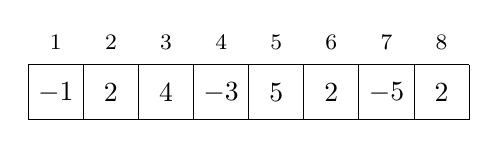
\begin{tikzpicture}[scale=0.7]
\draw (0,0) grid (8,1);

\node at (0.5,0.5) {$-1$};
\node at (1.5,0.5) {$2$};
\node at (2.5,0.5) {$4$};
\node at (3.5,0.5) {$-3$};
\node at (4.5,0.5) {$5$};
\node at (5.5,0.5) {$2$};
\node at (6.5,0.5) {$-5$};
\node at (7.5,0.5) {$2$};

\footnotesize
\node at (0.5,1.4) {$1$};
\node at (1.5,1.4) {$2$};
\node at (2.5,1.4) {$3$};
\node at (3.5,1.4) {$4$};
\node at (4.5,1.4) {$5$};
\node at (5.5,1.4) {$6$};
\node at (6.5,1.4) {$7$};
\node at (7.5,1.4) {$8$};
\end{tikzpicture}
\end{center}
optimiratkaisu on valita alitaulukko seuraavasti:
\begin{center}
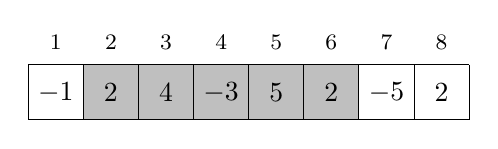
\begin{tikzpicture}[scale=0.7]
\fill[color=lightgray] (1,0) rectangle (6,1);
\draw (0,0) grid (8,1);

\node at (0.5,0.5) {$-1$};
\node at (1.5,0.5) {$2$};
\node at (2.5,0.5) {$4$};
\node at (3.5,0.5) {$-3$};
\node at (4.5,0.5) {$5$};
\node at (5.5,0.5) {$2$};
\node at (6.5,0.5) {$-5$};
\node at (7.5,0.5) {$2$};

\footnotesize
\node at (0.5,1.4) {$1$};
\node at (1.5,1.4) {$2$};
\node at (2.5,1.4) {$3$};
\node at (3.5,1.4) {$4$};
\node at (4.5,1.4) {$5$};
\node at (5.5,1.4) {$6$};
\node at (6.5,1.4) {$7$};
\node at (7.5,1.4) {$8$};
\end{tikzpicture}
\end{center}

Tämän alitaulukon summa on $2+4+(-3)+5+2=10$,
joka on suurin mahdollinen alitaulukon summa.
Tässä tapauksessa kannattaa ottaa mukaan summaan
luku $-3$, koska sen molemmilla puolilla
olevat luvut kasvattavat summaa.

\subsubsection{Ratkaisu 1}

Suoraviivainen ratkaisu tehtävään on käydä
läpi kaikki tavat valita alitaulukko taulukosta,
laskea jokaisesta vaihtoehdosta lukujen summa
ja pitää muistissa suurinta summaa.
Seuraava koodi toteuttaa tämän algoritmin:

\begin{lstlisting}
int p = 0;
for (int a = 1; a <= n; a++) {
    for (int b = a; b <= n; b++) {
        int s = 0;
        for (int c = a; c <= b; c++) {
            s += t[c];
        }
        p = max(p,s);
    }
}
cout << p << "\n";
\end{lstlisting}

Koodi olettaa, että luvut on tallennettu taulukkoon \texttt{t},
jota indeksoidaan $1 \ldots n$.
Muuttujat $a$ ja $b$ valitsevat alitaulukon ensimmäisen
ja viimeisen luvun, ja alitaulukon summa lasketaan muuttujaan $s$.
Muuttujassa $p$ on puolestaan paras haun aikana löydetty summa.

Algoritmin aikavaativuus on $O(n^3)$, koska siinä on kolme
sisäkkäistä silmukkaa ja jokainen silmukka käy läpi $O(n)$ lukua.

\subsubsection{Ratkaisu 2}

Äskeistä ratkaisua on helppoa tehostaa hankkiutumalla
eroon sisimmästä silmukasta.
Tämä on mahdollista laskemalla summaa samalla,
kun alitaulukon oikea reuna liikkuu eteenpäin.
Tuloksena on seuraava koodi:

\begin{lstlisting}
int p = 0;
for (int a = 1; a <= n; a++) {
    int s = 0;
    for (int b = a; b <= n; b++) {
        s += t[b];
        p = max(p,s);
    }
}
cout << p << "\n";
\end{lstlisting}
Tämän muutoksen jälkeen koodin aikavaativuus on $O(n^2)$.

\subsubsection{Ratkaisu 3}

Yllättävää kyllä, tehtävään on olemassa myös
$O(n)$-aikainen ratkaisu eli koodista pystyy
karsimaan vielä yhden silmukan.
Ratkaisun ideana on laskea taulukon jokaiseen
kohtaan, mikä on suurin mahdollinen summa
kyseiseen kohtaan päättyvässä alitaulukossa,
ja valita suurin näistä summista.

Kun alitaulukon loppukohta $k$ on valittu,
summan muodostamiseen on kaksi vaihtoehtoa.
Yksi mahdollisuus on, että summassa
on vain yksi luku: kohdassa $k$ oleva luku.
Muussa tapauksessa summassa on ensin
kohtaan $k-1$ päättyvän alitaulukon
summa ja sitten kohdassa $k$ oleva luku.

Koska tavoitteena on saada aikaan mahdollisimman
suuri summa, jälkimmäisessä tapauksessa myös
kohtaan $k-1$ päättyvän alitaulukon summa tulee valita niin,
että se on mahdollisimman suuri.
Niinpä tehokas ratkaisu syntyy käymällä läpi
kaikki loppukohdat $k$ järjestyksessä.

Seuraava koodi toteuttaa ratkaisun:

\begin{lstlisting}
int p = 0, s = 0;
for (int k = 1; k <= n; k++) {
    s = max(t[k],s+t[k]);
    p = max(p,s);
}
cout << p << "\n";
\end{lstlisting}

Algoritmissa on vain yksi silmukka,
joka käy läpi taulukon luvut,
joten sen aikavaativuus on $O(n)$.
Tämä on myös paras mahdollinen aikavaativuus,
koska minkä tahansa algoritmin täytyy käydä
läpi ainakin kerran taulukon sisältö.

\subsubsection{Tehokkuusvertailu}

On kiinnostavaa tutkia, kuinka tehokkaita algoritmit
ovat käytännössä.
Seuraava taulukko näyttää, kuinka nopeasti äskeiset
ratkaisut toimivat eri $n$:n arvoilla
nykyaikaisella tietokoneella.

Jokainen syöte on muodostettu satunnaisesti,
ja taulukon luvut ovat välillä $-10^9 \ldots 10^9$.
Ajankäyttöön ei ole laskettu syötteen lukemiseen
kuluvaa aikaa.

\begin{center}
\begin{tabular}{rrrr}
taulukon koko $n$ & ratkaisu 1 & ratkaisu 2 & ratkaisu 3 \\
\hline
$10^2$ & $0{,}0$ s & $0{,}0$ s & $0{,}0$ s \\
$10^3$ & $0{,}1$ s & $0{,}0$ s & $0{,}0$ s \\
$10^4$ & > $10,0$ s & $0{,}1$ s & $0{,}0$ s \\
$10^5$ & > $10,0$ s & $5{,}3$ s & $0{,}0$ s \\
$10^6$ & > $10,0$ s & > $10,0$ s & $0{,}0$ s \\
$10^7$ & > $10,0$ s & > $10,0$ s & $0{,}0$ s \\
\end{tabular}
\end{center}

Vertailu osoittaa,
että pienillä syötteillä kaikki algoritmit
ovat tehokkaita,
mutta suuremmat syötteet tuovat esille
huomattavia eroja algoritmien suoritusajassa.
$O(n)$-aikainen ratkaisu 3 on ainoa,
joka pystyy ratkaisemaan kaikki syötteet
alle 10 sekunnissa.


\chapter{Järjestäminen}

\index{jxrjestxminen@järjestäminen}

\key{Järjestäminen}
on keskeinen algoritmiikan ongelma.
Moni tehokas algoritmi
perustuu järjestämiseen,
koska järjestetyn tiedon
käsittely on helpompaa
kuin sekalaisessa järjestyksessä olevan.

Esimerkiksi kysymys ''onko taulukossa kahta samaa
alkiota?'' ratkeaa tehokkaasti järjestämisen avulla.
Jos taulukossa on kaksi samaa alkiota,
ne ovat järjestämisen jälkeen peräkkäin,
jolloin niiden löytäminen on helppoa.
Samaan tapaan ratkeaa myös kysymys
''mikä on yleisin alkio taulukossa?''.

Järjestämiseen on kehitetty monia
algoritmeja, jotka tarjoavat hyviä
esimerkkejä algoritmien suunnittelun tekniikoista.
Tehokkaat yleiset järjestämis\-algoritmit
toimivat ajassa $O(n \log n)$, ja tämä aikavaativuus
on myös monella järjestämistä käyttävällä algoritmilla.

\section{Järjestämisen teoriaa}

Järjestämisen perusongelma on seuraava:

\begin{task}
Annettuna on taulukko, jossa on $n$ alkiota.
Tehtäväsi on järjestää alkiot pienimmästä
suurimpaan.
\end{task}

\noindent
Esimerkiksi taulukko

\begin{center}
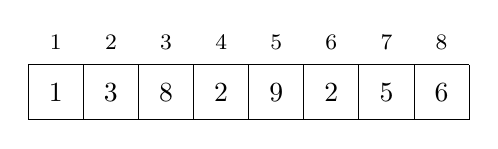
\begin{tikzpicture}[scale=0.7]
\draw (0,0) grid (8,1);
\node at (0.5,0.5) {$1$};
\node at (1.5,0.5) {$3$};
\node at (2.5,0.5) {$8$};
\node at (3.5,0.5) {$2$};
\node at (4.5,0.5) {$9$};
\node at (5.5,0.5) {$2$};
\node at (6.5,0.5) {$5$};
\node at (7.5,0.5) {$6$};

\footnotesize
\node at (0.5,1.4) {$1$};
\node at (1.5,1.4) {$2$};
\node at (2.5,1.4) {$3$};
\node at (3.5,1.4) {$4$};
\node at (4.5,1.4) {$5$};
\node at (5.5,1.4) {$6$};
\node at (6.5,1.4) {$7$};
\node at (7.5,1.4) {$8$};
\end{tikzpicture}
\end{center}

\noindent
on järjestettynä seuraava:

\begin{center}
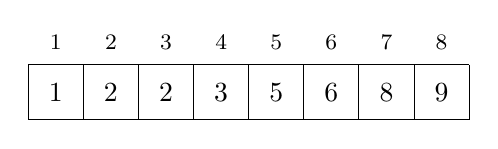
\begin{tikzpicture}[scale=0.7]
\draw (0,0) grid (8,1);
\node at (0.5,0.5) {$1$};
\node at (1.5,0.5) {$2$};
\node at (2.5,0.5) {$2$};
\node at (3.5,0.5) {$3$};
\node at (4.5,0.5) {$5$};
\node at (5.5,0.5) {$6$};
\node at (6.5,0.5) {$8$};
\node at (7.5,0.5) {$9$};

\footnotesize
\node at (0.5,1.4) {$1$};
\node at (1.5,1.4) {$2$};
\node at (2.5,1.4) {$3$};
\node at (3.5,1.4) {$4$};
\node at (4.5,1.4) {$5$};
\node at (5.5,1.4) {$6$};
\node at (6.5,1.4) {$7$};
\node at (7.5,1.4) {$8$};
\end{tikzpicture}
\end{center}

\subsubsection{$O(n^2)$-algoritmit}

\index{kuplajxrjestxminen@kuplajärjestäminen}

Yksinkertaiset algoritmit taulukon
järjestämiseen vievät aikaa $O(n^2)$.
Ehkä tunnetuin tällainen algoritmi on
\key{kuplajärjestäminen} (''bubble sort''),
joka muodostuu peräkkäisistä taulukon läpikäynneistä.

Algoritmissa jokainen taulukon läpikäynti
etsii vierekkäisiä alkiopareja,
jotka ovat väärässä järjestyksessä,
ja korjaa näiden alkioparien järjestyksen.
Algoritmi päättyy, kun läpikäynnin
aikana ei tule mitään muutoksia taulukkoon,
jolloin taulukko on järjestyksessä.

Kuplajärjestämisen voi toteuttaa seuraavasti,
kun järjestettävä taulukko muodostuu alkioista
$\texttt{t}[1],\texttt{t}[2],\ldots,\texttt{t}[n]$:
\begin{lstlisting}
bool stop = false;
while (!stop) {
    stop = true;
    for (int i = 1; i <= n-1; i++) {
        if (t[i] > t[i+1]) {
            swap(t[i],t[i+1]);
            stop = false;
        }
    }
}
\end{lstlisting}

\noindent
Esimerkiksi taulukossa

\begin{center}
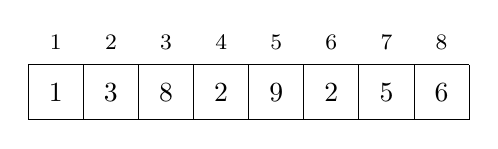
\begin{tikzpicture}[scale=0.7]
\draw (0,0) grid (8,1);

\node at (0.5,0.5) {$1$};
\node at (1.5,0.5) {$3$};
\node at (2.5,0.5) {$8$};
\node at (3.5,0.5) {$2$};
\node at (4.5,0.5) {$9$};
\node at (5.5,0.5) {$2$};
\node at (6.5,0.5) {$5$};
\node at (7.5,0.5) {$6$};

\footnotesize
\node at (0.5,1.4) {$1$};
\node at (1.5,1.4) {$2$};
\node at (2.5,1.4) {$3$};
\node at (3.5,1.4) {$4$};
\node at (4.5,1.4) {$5$};
\node at (5.5,1.4) {$6$};
\node at (6.5,1.4) {$7$};
\node at (7.5,1.4) {$8$};
\end{tikzpicture}
\end{center}

\noindent
kuplajärjestämisen ensimmäinen
läpikäynti tekee seuraavat vaihdot:

\begin{center}
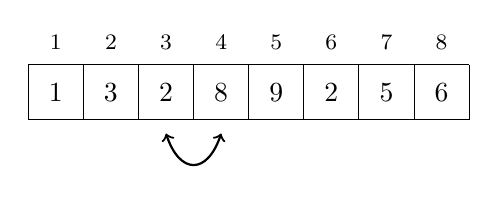
\begin{tikzpicture}[scale=0.7]
\draw (0,0) grid (8,1);
\node at (0.5,0.5) {$1$};
\node at (1.5,0.5) {$3$};
\node at (2.5,0.5) {$2$};
\node at (3.5,0.5) {$8$};
\node at (4.5,0.5) {$9$};
\node at (5.5,0.5) {$2$};
\node at (6.5,0.5) {$5$};
\node at (7.5,0.5) {$6$};

\draw[thick,<->] (3.5,-0.25) .. controls (3.25,-1.00) and (2.75,-1.00) .. (2.5,-0.25);

\footnotesize
\node at (0.5,1.4) {$1$};
\node at (1.5,1.4) {$2$};
\node at (2.5,1.4) {$3$};
\node at (3.5,1.4) {$4$};
\node at (4.5,1.4) {$5$};
\node at (5.5,1.4) {$6$};
\node at (6.5,1.4) {$7$};
\node at (7.5,1.4) {$8$};
\end{tikzpicture}
\end{center}

\begin{center}
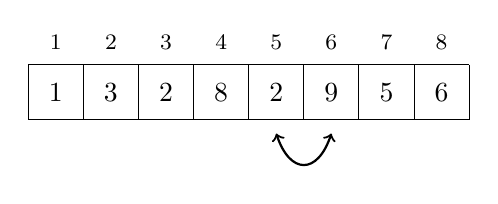
\begin{tikzpicture}[scale=0.7]
\draw (0,0) grid (8,1);
\node at (0.5,0.5) {$1$};
\node at (1.5,0.5) {$3$};
\node at (2.5,0.5) {$2$};
\node at (3.5,0.5) {$8$};
\node at (4.5,0.5) {$2$};
\node at (5.5,0.5) {$9$};
\node at (6.5,0.5) {$5$};
\node at (7.5,0.5) {$6$};

\draw[thick,<->] (5.5,-0.25) .. controls (5.25,-1.00) and (4.75,-1.00) .. (4.5,-0.25);


\footnotesize
\node at (0.5,1.4) {$1$};
\node at (1.5,1.4) {$2$};
\node at (2.5,1.4) {$3$};
\node at (3.5,1.4) {$4$};
\node at (4.5,1.4) {$5$};
\node at (5.5,1.4) {$6$};
\node at (6.5,1.4) {$7$};
\node at (7.5,1.4) {$8$};
\end{tikzpicture}
\end{center}

\begin{center}
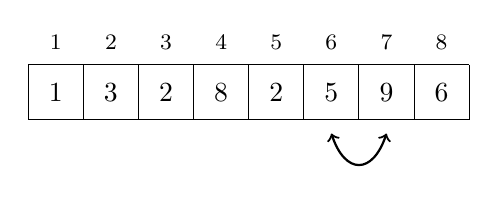
\begin{tikzpicture}[scale=0.7]
\draw (0,0) grid (8,1);
\node at (0.5,0.5) {$1$};
\node at (1.5,0.5) {$3$};
\node at (2.5,0.5) {$2$};
\node at (3.5,0.5) {$8$};
\node at (4.5,0.5) {$2$};
\node at (5.5,0.5) {$5$};
\node at (6.5,0.5) {$9$};
\node at (7.5,0.5) {$6$};

\draw[thick,<->] (6.5,-0.25) .. controls (6.25,-1.00) and (5.75,-1.00) .. (5.5,-0.25);


\footnotesize
\node at (0.5,1.4) {$1$};
\node at (1.5,1.4) {$2$};
\node at (2.5,1.4) {$3$};
\node at (3.5,1.4) {$4$};
\node at (4.5,1.4) {$5$};
\node at (5.5,1.4) {$6$};
\node at (6.5,1.4) {$7$};
\node at (7.5,1.4) {$8$};
\end{tikzpicture}
\end{center}

\begin{center}
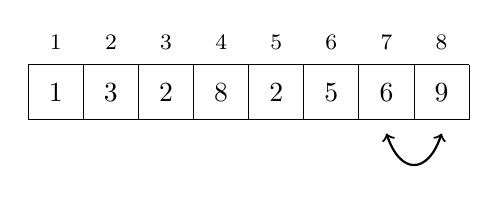
\begin{tikzpicture}[scale=0.7]
\draw (0,0) grid (8,1);
\node at (0.5,0.5) {$1$};
\node at (1.5,0.5) {$3$};
\node at (2.5,0.5) {$2$};
\node at (3.5,0.5) {$8$};
\node at (4.5,0.5) {$2$};
\node at (5.5,0.5) {$5$};
\node at (6.5,0.5) {$6$};
\node at (7.5,0.5) {$9$};

\draw[thick,<->] (7.5,-0.25) .. controls (7.25,-1.00) and (6.75,-1.00) .. (6.5,-0.25);

\footnotesize
\node at (0.5,1.4) {$1$};
\node at (1.5,1.4) {$2$};
\node at (2.5,1.4) {$3$};
\node at (3.5,1.4) {$4$};
\node at (4.5,1.4) {$5$};
\node at (5.5,1.4) {$6$};
\node at (6.5,1.4) {$7$};
\node at (7.5,1.4) {$8$};
\end{tikzpicture}
\end{center}


Kuplajärjestämisessä ensimmäisen läpikäynnin jälkeen suurin alkio
on paikallaan, toisen läpikäynnin jälkeen
kaksi suurinta alkiota on paikallaan, jne.
Niinpä kuplajärjestäminen päättyy aina viimeistään $n$
läpikäynnin jälkeen.
Koska jokainen läpikäynti vie aikaa $O(n)$,
algoritmin aikavaativuus on $O(n^2)$.

\subsubsection{Inversiot}

\index{inversio@inversio}

Kuplajärjestäminen on esimerkki algoritmista,
joka perustuu taulukon vierekkäisten alkioiden
vaihtamiseen.
Osoittautuu, että minkään tällaisen algoritmin
aikavaativuus ei voi olla parempi kuin $O(n^2)$,
koska tarvittava vaihtojen määrä
saattaa olla luokkaa $O(n^2)$.

Hyödyllinen käsite järjestämisalgoritmien
analyysissa on \key{inversio}.
Se on indeksipari $(a,b)$, joille $a<b$
ja $\texttt{t}[a]>\texttt{t}[b]$
eli kaksi taulukon alkiota, jotka ovat väärässä
järjestyksessä.
Esimerkiksi taulukossa

\begin{center}
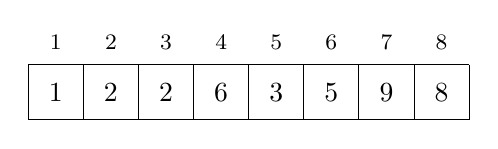
\begin{tikzpicture}[scale=0.7]
\draw (0,0) grid (8,1);
\node at (0.5,0.5) {$1$};
\node at (1.5,0.5) {$2$};
\node at (2.5,0.5) {$2$};
\node at (3.5,0.5) {$6$};
\node at (4.5,0.5) {$3$};
\node at (5.5,0.5) {$5$};
\node at (6.5,0.5) {$9$};
\node at (7.5,0.5) {$8$};

\footnotesize
\node at (0.5,1.4) {$1$};
\node at (1.5,1.4) {$2$};
\node at (2.5,1.4) {$3$};
\node at (3.5,1.4) {$4$};
\node at (4.5,1.4) {$5$};
\node at (5.5,1.4) {$6$};
\node at (6.5,1.4) {$7$};
\node at (7.5,1.4) {$8$};
\end{tikzpicture}
\end{center}

inversiot ovat $(4,5)$, $(4,6)$ ja $(7,8)$.
Inversioiden määrä kuvaa, miten lähellä
järjestystä taulukko on.
Järjestetyn taulukon inversioiden määrä on 0,
ja käänteisesti järjestetyn taulukon
inversioiden määrä on $1+2+\cdots+(n-1)=\frac{n(n-1)}{2}$.

Jos vierekkäiset alkiot ovat väärässä järjestyksessä,
niiden vaihtaminen keskenään poistaa
taulukosta yhden inversion.
Niinpä inversioiden määrä on sama kuin
taulukon järjestämiseen tarvittava vaihtojen määrä.
Vierekkäisiä alkioita
vaihtavan algoritmin aikavaativuus
on aina ainakin $O(n^2)$,
koska sen täytyy tehdä pahimmassa tapauksessa
$\frac{n(n-1)}{2} = O(n^2)$ vaihtoa.

\subsubsection{$O(n \log n)$-algoritmit}

\index{lomitusjxrjestxminen@lomitusjärjestäminen}

Tehokkaat järjestämisalgoritmit vievät
aikaa $O(n \log n)$.
Yksi tällainen algoritmi on
\key{lomitusjärjestäminen} (''merge sort''),
joka järjestää taulukon
rekursiivisesti jakamalla sen
pienemmiksi osataulukoiksi.

Lomitusjärjestäminen
jakaa taulukon kahdeksi osataulukoksi,
järjestää osataulukot rekursiivisesti ja muodostaa
sitten järjestetyn taulukon yhdistämällä osataulukot.
Algoritmin runko on seuraava:
\begin{lstlisting}
void mergesort(int a, int b) {
    if (a == b) return;
    int c = (a+b)/2;
    mergesort(a,c);
    mergesort(c+1,b);
    merge(a,c,c+1,b);
}
\end{lstlisting}
Funktio \texttt{mergesort}
järjestää taulukon välin $a \ldots b$ alkiot.
Jos $a=b$, välillä on vain yksi alkio,
joten se on valmiiksi järjestyksessä.
Muuten algoritmi jakaa välin
kahteen osaan: vasen osa on väli $a \ldots c$
ja oikea osa on väli $c+1 \ldots b$, missä $c=(a+b)/2$.
Algoritmi järjestää osat rekursiivisesti
kutsumalla itseään.

Algoritmi kutsuu funktiota \texttt{merge},
joka lomittaa välin vasemman ja oikean osan alkiot.
Tämä tarkoittaa, että alkiot kerätään yhteen niin,
että koko taulukon väli on järjestyksessä.
Lomitus
on mahdollista toteuttaa ajassa $O(n)$
valitsemalla alkiot järjestyksessä vasemman ja
oikean osan alusta alkaen.

\begin{samepage}
Esimerkiksi taulukko

\begin{center}
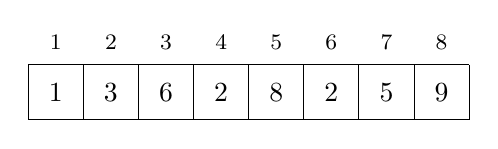
\begin{tikzpicture}[scale=0.7]
\draw (0,0) grid (8,1);
\node at (0.5,0.5) {$1$};
\node at (1.5,0.5) {$3$};
\node at (2.5,0.5) {$6$};
\node at (3.5,0.5) {$2$};
\node at (4.5,0.5) {$8$};
\node at (5.5,0.5) {$2$};
\node at (6.5,0.5) {$5$};
\node at (7.5,0.5) {$9$};

\footnotesize
\node at (0.5,1.4) {$1$};
\node at (1.5,1.4) {$2$};
\node at (2.5,1.4) {$3$};
\node at (3.5,1.4) {$4$};
\node at (4.5,1.4) {$5$};
\node at (5.5,1.4) {$6$};
\node at (6.5,1.4) {$7$};
\node at (7.5,1.4) {$8$};
\end{tikzpicture}
\end{center}
\end{samepage}

jakautuu osataulukoiksi

\begin{center}
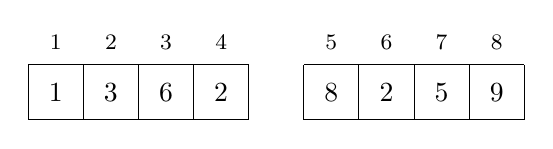
\begin{tikzpicture}[scale=0.7]
\draw (0,0) grid (4,1);
\draw (5,0) grid (9,1);

\node at (0.5,0.5) {$1$};
\node at (1.5,0.5) {$3$};
\node at (2.5,0.5) {$6$};
\node at (3.5,0.5) {$2$};

\node at (5.5,0.5) {$8$};
\node at (6.5,0.5) {$2$};
\node at (7.5,0.5) {$5$};
\node at (8.5,0.5) {$9$};

\footnotesize
\node at (0.5,1.4) {$1$};
\node at (1.5,1.4) {$2$};
\node at (2.5,1.4) {$3$};
\node at (3.5,1.4) {$4$};
\node at (5.5,1.4) {$5$};
\node at (6.5,1.4) {$6$};
\node at (7.5,1.4) {$7$};
\node at (8.5,1.4) {$8$};

\end{tikzpicture}
\end{center}

jotka ovat järjestettyinä:

\begin{center}
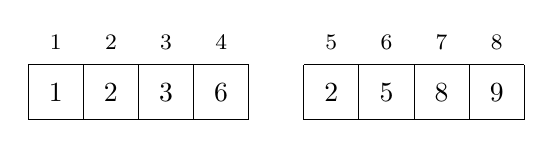
\begin{tikzpicture}[scale=0.7]
\draw (0,0) grid (4,1);
\draw (5,0) grid (9,1);

\node at (0.5,0.5) {$1$};
\node at (1.5,0.5) {$2$};
\node at (2.5,0.5) {$3$};
\node at (3.5,0.5) {$6$};

\node at (5.5,0.5) {$2$};
\node at (6.5,0.5) {$5$};
\node at (7.5,0.5) {$8$};
\node at (8.5,0.5) {$9$};

\footnotesize
\node at (0.5,1.4) {$1$};
\node at (1.5,1.4) {$2$};
\node at (2.5,1.4) {$3$};
\node at (3.5,1.4) {$4$};
\node at (5.5,1.4) {$5$};
\node at (6.5,1.4) {$6$};
\node at (7.5,1.4) {$7$};
\node at (8.5,1.4) {$8$};
\end{tikzpicture}
\end{center}

Osataulukot lomittamalla syntyy järjestetty taulukko

\begin{center}
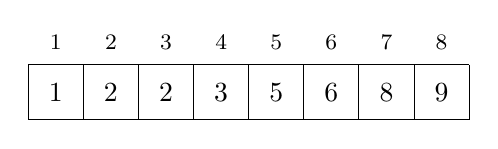
\begin{tikzpicture}[scale=0.7]
\draw (0,0) grid (8,1);
\node at (0.5,0.5) {$1$};
\node at (1.5,0.5) {$2$};
\node at (2.5,0.5) {$2$};
\node at (3.5,0.5) {$3$};
\node at (4.5,0.5) {$5$};
\node at (5.5,0.5) {$6$};
\node at (6.5,0.5) {$8$};
\node at (7.5,0.5) {$9$};

\footnotesize
\node at (0.5,1.4) {$1$};
\node at (1.5,1.4) {$2$};
\node at (2.5,1.4) {$3$};
\node at (3.5,1.4) {$4$};
\node at (4.5,1.4) {$5$};
\node at (5.5,1.4) {$6$};
\node at (6.5,1.4) {$7$};
\node at (7.5,1.4) {$8$};
\end{tikzpicture}
\end{center}

Lomitusjärjestämisen aikavaativuus on $O(n \log n)$,
koska algoritmin aikana
osataulukoista muodostuu $O(\log n)$ tasoa
ja kullakin tasolla osataulukoiden lomitus
vie yhteensä $O(n)$ aikaa.

\subsubsection{Järjestämisen alaraja}

Monet järjestämisalgoritmi saavuttavat
aikavaativuuden $O(n \log n)$,
mutta kukaan ei ole onnistunut keksimään
yleistä järjestämisalgoritmia,
joka toimisi nopeammin kuin $O(n \log n)$.
Tähän on yllättävä syy: on mahdollista todistaa,
että tällaista algoritmia ei ole olemassa.

Ideana todistuksessa on tarkastella järjestämistä
prosessina, jossa jokainen kahden alkion vertailu
antaa lisää tietoa taulukon sisällöstä.
Prosessista muodostuu seuraavanlainen puu:

\begin{center}
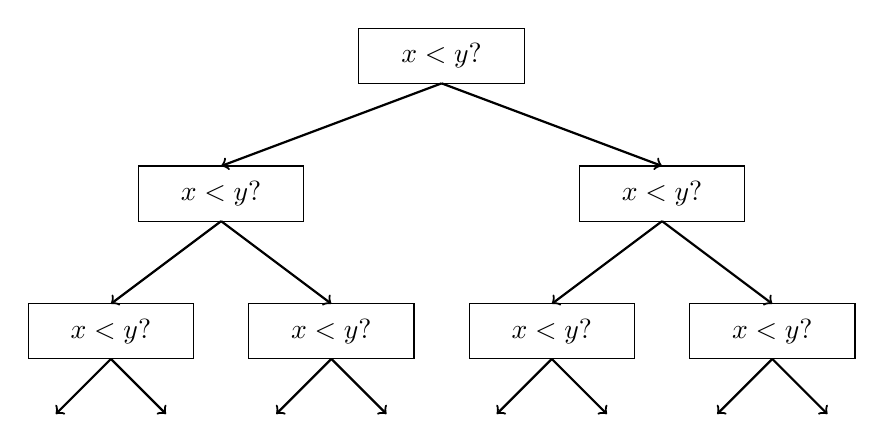
\begin{tikzpicture}[scale=0.7]
\draw (0,0) rectangle (3,1);
\node at (1.5,0.5) {$x < y?$};

\draw[thick,->] (1.5,0) -- (-2.5,-1.5);
\draw[thick,->] (1.5,0) -- (5.5,-1.5);

\draw (-4,-2.5) rectangle (-1,-1.5);
\draw (4,-2.5) rectangle (7,-1.5);
\node at (-2.5,-2) {$x < y?$};
\node at (5.5,-2) {$x < y?$};

\draw[thick,->] (-2.5,-2.5) -- (-4.5,-4);
\draw[thick,->] (-2.5,-2.5) -- (-0.5,-4);
\draw[thick,->] (5.5,-2.5) -- (3.5,-4);
\draw[thick,->] (5.5,-2.5) -- (7.5,-4);

\draw (-6,-5) rectangle (-3,-4);
\draw (-2,-5) rectangle (1,-4);
\draw (2,-5) rectangle (5,-4);
\draw (6,-5) rectangle (9,-4);
\node at (-4.5,-4.5) {$x < y?$};
\node at (-0.5,-4.5) {$x < y?$};
\node at (3.5,-4.5) {$x < y?$};
\node at (7.5,-4.5) {$x < y?$};

\draw[thick,->] (-4.5,-5) -- (-5.5,-6);
\draw[thick,->] (-4.5,-5) -- (-3.5,-6);
\draw[thick,->] (-0.5,-5) -- (0.5,-6);
\draw[thick,->] (-0.5,-5) -- (-1.5,-6);
\draw[thick,->] (3.5,-5) -- (2.5,-6);
\draw[thick,->] (3.5,-5) -- (4.5,-6);
\draw[thick,->] (7.5,-5) -- (6.5,-6);
\draw[thick,->] (7.5,-5) -- (8.5,-6);
\end{tikzpicture}
\end{center}

Merkintä ''$x<y?$'' tarkoittaa taulukon alkioiden
$x$ ja $y$ vertailua.
Jos $x<y$, prosessi jatkaa vasemmalle,
ja muuten oikealle.
Prosessin tulokset ovat taulukon mahdolliset
järjestykset, joita on kaikkiaan $n!$ erilaista.
Puun korkeuden tulee olla tämän vuoksi vähintään

\[ \log_2(n!) = \log_2(1)+\log_2(2)+\cdots+\log_2(n) = O(n \log n).\]

\subsubsection{Laskemisjärjestäminen}

\index{laskemisjxrjestxminen@laskemisjärjestäminen}

Järjestämisen alaraja $O(n \log n)$ ei koske algoritmeja,
jotka eivät perustu alkioiden vertailuun vaan hyödyntävät
jotain muuta tietoa alkioista.
Esimerkki tällaisesta algoritmista on
\key{laskemisjärjestäminen}, joka järjestää
kokonaisluvuista koostuvan taulukon $O(n)$-ajassa.

Algoritmin ideana on luoda \emph{kirjanpito}, josta selviää,
montako kertaa mikäkin alkio esiintyy taulukossa.
Kirjanpito on taulukko, jonka indeksit ovat alkuperäisen
taulukon alkioita.
Jokaisen indeksin kohdalla lukee, montako kertaa
kyseinen alkio esiintyy alkuperäisessä taulukossa.

Esimerkiksi taulukosta

\begin{center}
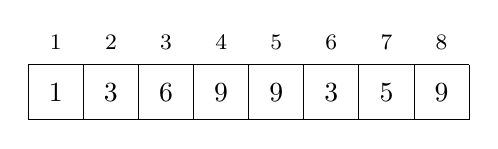
\begin{tikzpicture}[scale=0.7]
\draw (0,0) grid (8,1);
\node at (0.5,0.5) {$1$};
\node at (1.5,0.5) {$3$};
\node at (2.5,0.5) {$6$};
\node at (3.5,0.5) {$9$};
\node at (4.5,0.5) {$9$};
\node at (5.5,0.5) {$3$};
\node at (6.5,0.5) {$5$};
\node at (7.5,0.5) {$9$};

\footnotesize
\node at (0.5,1.4) {$1$};
\node at (1.5,1.4) {$2$};
\node at (2.5,1.4) {$3$};
\node at (3.5,1.4) {$4$};
\node at (4.5,1.4) {$5$};
\node at (5.5,1.4) {$6$};
\node at (6.5,1.4) {$7$};
\node at (7.5,1.4) {$8$};
\end{tikzpicture}
\end{center}

syntyy seuraava kirjanpito:

\begin{center}
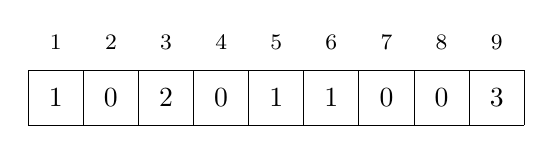
\begin{tikzpicture}[scale=0.7]
\draw (0,0) grid (9,1);
\node at (0.5,0.5) {$1$};
\node at (1.5,0.5) {$0$};
\node at (2.5,0.5) {$2$};
\node at (3.5,0.5) {$0$};
\node at (4.5,0.5) {$1$};
\node at (5.5,0.5) {$1$};
\node at (6.5,0.5) {$0$};
\node at (7.5,0.5) {$0$};
\node at (8.5,0.5) {$3$};

\footnotesize

\node at (0.5,1.5) {$1$};
\node at (1.5,1.5) {$2$};
\node at (2.5,1.5) {$3$};
\node at (3.5,1.5) {$4$};
\node at (4.5,1.5) {$5$};
\node at (5.5,1.5) {$6$};
\node at (6.5,1.5) {$7$};
\node at (7.5,1.5) {$8$};
\node at (8.5,1.5) {$9$};
\end{tikzpicture}
\end{center}

Esimerkiksi kirjanpidossa lukee indeksin 3 kohdalla 2,
koska luku 3 esiintyy kahdesti alkuperäisessä
taulukossa (indekseissä 2 ja 6).

Kirjanpidon muodostus vie aikaa $O(n)$,
koska riittää käydä taulukko läpi kerran.
Tämän jälkeen järjestetyn taulukon luominen
vie myös aikaa $O(n)$, koska kunkin alkion
määrän saa selville suoraan kirjanpidosta.
Niinpä laskemisjärjestämisen
kokonaisaikavaativuus on $O(n)$.

Laskemisjärjestäminen on hyvin tehokas algoritmi,
mutta sen käyttäminen vaatii,
että taulukon sisältönä on niin pieniä
kokonaislukuja, että niitä voi käyttää
kirjanpidon taulukon indeksöinnissä.

\section{Järjestäminen C++:ssa}

\index{sort@\texttt{sort}}

C++:n standardikirjastossa on funktio \texttt{sort},
jonka avulla voi järjestää helposti taulukoita
ja muita tietorakenteita.
Tätä funktiota kannattaa käyttää yleensä aina
järjestämiseen algoritmeissa,
koska funktio on toteutettu tehokkaasti ja varmasti toimivasti.

\begin{minipage}{\textwidth}
Seuraava koodi järjestää vektorin \texttt{v}
luvut pienimmästä suurimpaan:

\begin{lstlisting}
vector<int> v = {4,2,5,3,5,8,3};
sort(v.begin(),v.end());
\end{lstlisting}
\end{minipage}

Järjestämisen jälkeen vektorin sisältö on
$\{2,3,3,4,5,5,8\}$.

Oletuksena järjestys tapahtuu pienimmästä suurimpaan,
mutta järjestyksen saa käänteiseksi näin:

\begin{lstlisting}
sort(v.rbegin(),v.rend());
\end{lstlisting}

Tavallisen taulukon voi järjestää seuraavasti:

\begin{lstlisting}
int n = 7; // taulukon koko
int t[] = {4,2,5,3,5,8,3};
sort(t,t+n);
\end{lstlisting}

Seuraava koodi järjestää merkkijonon \texttt{s}:

\begin{lstlisting}
string s = "apina";
sort(s.begin(), s.end());
\end{lstlisting}

Merkkijonon järjestäminen tarkoittaa,
että sen merkit järjestetään aakkosjärjestykseen.
Esimerkiksi merkkijono ''apina''
on järjestettynä ''aainp''.

\subsubsection{Vertailuoperaattori}

\index{vertailuoperaattori@vertailuoperaattori}

Funktion \texttt{sort} käyttäminen vaatii,
että järjestettävien alkioiden
tietotyypille on määritelty \key{vertailuoperaattori} \texttt{<},
jonka avulla voi selvittää, mikä on kahden alkion järjestys.
Järjestämisen aikana \texttt{sort}-funktio
käyttää operaattoria \texttt{<} aina, kun sen täytyy
vertailla järjestettäviä alkioita.

Vertailuoperaattori on määritelty valmiiksi
useimmille C++:n tietotyypeille,
minkä ansiosta niitä pystyy järjestämään automaattisesti.
Jos järjestettävänä on lukuja, ne järjestyvät
suuruusjärjestykseen,
ja jos järjestettävänä on merkkijonoja,
ne järjestyvät aakkosjärjestykseen.

Parit (\texttt{pair}) järjestyvät ensisijaisesti
ensimmäisen kentän (\texttt{first}) mukaan.
Jos kuitenkin parien ensimmäiset kentät ovat samat,
järjestys määräytyy toisen kentän (\texttt{second}) mukaan.
Seuraava koodi esittelee asiaa:

\begin{lstlisting}
vector<pair<int,int>> v;
v.push_back({1,5});
v.push_back({2,3});
v.push_back({1,2});
sort(v.begin(), v.end());
\end{lstlisting}

Koodin suorituksen jälkeen parien järjestys on
$(1,2)$, $(1,5)$, $(2,3)$.

Jos järjestettävänä on omia tietueita,
niiden vertailuoperaattori täytyy toteuttaa itse.
Operaattori määritellään tietueen sisään
\texttt{operator<}-nimisenä funktiona,
jonka parametrina on toinen alkio.
Operaattorin tulee palauttaa \texttt{true},
jos oma alkio on pienempi kuin parametrialkio,
ja muuten \texttt{false}.

Esimerkiksi seuraava tietue \texttt{P}
sisältää pisteen x- ja y-koordinaatit.
Vertailuoperaattori on toteutettu niin,
että pisteet järjestyvät ensisijaisesti x-koor\-di\-naa\-tin
ja toissijaisesti y-koordinaatin mukaan.

\begin{lstlisting}
struct P {
    int x, y;
    bool operator<(const p& a) {
        if (this.x != a.x) return this.x < a.x;
        else return this.y < a.y;
    }
};
\end{lstlisting}

\subsubsection{Vertailufunktio}

\index{vertailufunktio@vertailufunktio}

On myös mahdollista antaa
\texttt{sort}-funktiolle ulkopuolinen \key{vertailufunktio}.
Esimerkiksi seuraava vertailufunktio
järjestää merkkijonot ensisijaisesti pituuden mukaan
ja toissijaisesti aakkosjärjestyksen mukaan:

\begin{lstlisting}
bool cmp(string a, string b) {
    if (a.size() != b.size()) return a.size() < b.size();
    return a < b;
}
\end{lstlisting}

Tämän jälkeen merkkijonovektorin voi järjestää näin:

\begin{lstlisting}
sort(v.begin(), v.end(), cmp);
\end{lstlisting}

\section{Binäärihaku}

\index{binxxrihaku@binäärihaku}

Tavallinen tapa etsiä alkiota $x$ taulukosta \texttt{t}
on käyttää \texttt{for}-silmukkaa, joka käy läpi
taulukon sisällön:

\begin{lstlisting}
for (int i = 1; i <= n; i++) {
    if (t[i] == x) // alkio x löytyi kohdasta i
}
\end{lstlisting}

Tämän menetelmän aikavaativuus on $O(n)$,
koska pahimmassa tapauksessa koko taulukko täytyy
käydä läpi.
Jos taulukon sisältö voi olla mitä tahansa,
tämä on kuitenkin tehokkain mahdollinen menetelmä,
koska saatavilla ei ole lisätietoa siitä,
mistä päin taulukkoa alkiota $x$ kannattaa etsiä.

Tilanne on toinen silloin, kun taulukko on
järjestyksessä.
Tässä tapauksessa haku on mahdollista toteuttaa
paljon nopeammin, koska alkioiden järjestys
ohjaa etsimään alkiota oikeasta suunnasta.
Seuraavaksi käsiteltävä \key{binäärihaku}
löytää alkion järjestetystä taulukosta
tehokkaasti ajassa $O(\log n)$.

\subsubsection{Toteutus 1}

Perinteinen tapa toteuttaa binäärihaku muistuttaa sanan etsimistä
sanakirjasta. Haku puolittaa joka askeleella hakualueen taulukossa,
kunnes lopulta etsittävä alkio löytyy tai osoittautuu,
että sitä ei ole taulukossa.

Haku tarkistaa ensin taulukon keskimmäisen alkion.
Jos keskimmäinen alkio on etsittävä alkio, haku päättyy.
Muuten haku jatkuu taulukon vasempaan tai oikeaan osaan sen mukaan,
onko keskimmäinen alkio suurempi vain pienempi kuin etsittävä alkio.

Yllä olevan idean voi toteuttaa seuraavasti:
\begin{lstlisting}
int a = 1, b = n;
while (a <= b) {
    int k = (a+b)/2;
    if (t[k] == x) // alkio x löytyi kohdasta k
    if (t[k] > x) b = k-1;
    else a = k+1;
}
\end{lstlisting}

Algoritmi pitää yllä väliä $a \ldots b$, joka on
jäljellä oleva hakualue taulukossa.
Aluksi väli on $1 \ldots n$ eli koko taulukko.
Välin koko puolittuu algoritmin joka vaiheessa,
joten aikavaativuus on $O(\log n)$.

\subsubsection{Toteutus 2}

Vaihtoehtoinen tapa toteuttaa binäärihaku
perustuu taulukon tehostettuun läpikäyntiin.
Ideana on käydä taulukkoa läpi hyppien
ja hidastaa vauhtia, kun etsittävä alkio lähestyy.

Haku käy taulukkoa läpi vasemmalta oikealle aloittaen
hypyn pituudesta $n$.
Joka vaiheessa hypyn pituus puolittuu:
ensin $n/2$, sitten $n/4$, sitten $n/8$ jne.,
kunnes lopulta hypyn pituus on 1.
Hyppyjen jälkeen joko haettava alkio on löytynyt
tai selviää, että sitä ei ole taulukossa.

Seuraava koodi toteuttaa äskeisen idean:
\begin{lstlisting}
int k = 1;
for (int b = n; b >= 1; b /= 2) {
    while (k+b <= n && t[k+b] <= x) k += b;
}
if (t[k] == x) // alkio x löytyi kohdasta k
\end{lstlisting}

Muuttuja $k$ on läpikäynnin kohta taulukossa
ja muuttuja $b$ on hypyn pituus.
Jos alkio $x$ esiintyy taulukossa,
sen kohta on muuttujassa $k$ algoritmin päätteeksi.
Algoritmin aikavaativuus on $O(\log n)$,
koska \texttt{while}-silmukassa oleva koodi suoritetaan
aina enintään kahdesti.

\subsubsection{Muutoskohdan etsiminen}

Käytännössä binäärihakua tarvitsee koodata
harvoin alkion etsimiseen taulukosta,
koska sen sijasta voi käyttää standardikirjastoa.
Esimerkiksi C++:n funktiot \texttt{lower\_bound}
ja \texttt{upper\_bound} toteuttavat binäärihaun
ja tietorakenne \texttt{set} ylläpitää joukkoa,
jonka operaatiot ovat $O(\log n)$-aikaisia.

Sitäkin tärkeämpi binäärihaun käyttökohde on 
funktion muutoskohdan etsiminen.
Oletetaan, että haluamme löytää pienimmän arvon $k$,
joka on kelvollinen ratkaisu ongelmaan.
Käytössämme on funktio $\texttt{ok}(x)$,
joka palauttaa \texttt{true}, jos $x$ on kelvollinen
ratkaisu, ja muuten \texttt{false}.
Lisäksi tiedämme, että $\texttt{ok}(x)$ on \texttt{false}
aina kun $x<k$ ja \texttt{true} aina kun $x \geq k$.

Toisin sanoen haluamme löytää funktion \texttt{ok} muutoskohdan,
jossa arvosta \texttt{false} tulee arvo \texttt{true}.
Tilanne näyttää seuraavalta:

\begin{center}
\begin{tabular}{r|rrrrrrrr}
$x$ & 0 & 1 & $\cdots$ & $k-1$ & $k$ & $k+1$ & $\cdots$ \\
\hline
$\texttt{ok}(x)$ & \texttt{false} & \texttt{false}
& $\cdots$ & \texttt{false} & \texttt{true} & \texttt{true} & $\cdots$ \\
\end{tabular}
\end{center}

\noindent
Nyt muutoskohta on mahdollista etsiä käyttämällä
binäärihakua:

\begin{lstlisting}
int x = -1;
for (int b = z; b >= 1; b /= 2) {
    while (!ok(x+b)) x += b;
}
int k = x+1;
\end{lstlisting}

Haku etsii suurimman $x$:n arvon,
jolla $\texttt{ok}(x)$ on \texttt{false}.
Niinpä tästä seuraava arvo $k=x+1$
on pienin arvo, jolla $\texttt{ok}(k)$ on \texttt{true}.
Hypyn aloituspituus $z$ tulee olla 
sopiva suuri luku, esimerkiksi sellainen,
jolla $\texttt{ok}(z)$ on varmasti \texttt{true}.

Algoritmi kutsuu $O(\log z)$ kertaa funktiota
\texttt{ok}, joten kokonaisaikavaativuus
riippuu siitä, kauanko funktion \texttt{ok}
suoritus kestää.
Esimerkiksi jos ratkaisun tarkastus
vie aikaa $O(n)$, niin kokonaisaikavaativuus
on $O(n \log z)$.

\subsubsection{Huippuarvon etsiminen}

Binäärihaulla voi myös etsiä
suurimman arvon funktiolle,
joka on ensin kasvava ja sitten laskeva.
Toisin sanoen tehtävänä on etsiä arvo
$k$ niin, että

\begin{itemize}
\item
$f(x)<f(x+1)$, kun $x<k$, ja
\item
$f(x)>f(x+1)$, kun $x >= k$.
\end{itemize}

Ideana on etsiä binäärihaulla
viimeinen kohta $x$,
jossa pätee $f(x)<f(x+1)$.
Tällöin $k=x+1$,
koska pätee $f(x+1)>f(x+2)$.
Seuraava koodi toteuttaa haun: 

\begin{lstlisting}
int x = -1;
for (int b = z; b >= 1; b /= 2) {
    while (f(x+b) < f(x+b+1)) x += b;
}
int k = x+1;
\end{lstlisting}

Huomaa, että toisin kuin tavallisessa binäärihaussa,
tässä ei ole sallittua,
että peräkkäiset arvot olisivat yhtä suuria.
Silloin ei olisi mahdollista tietää,
mihin suuntaan hakua tulee jatkaa.




\chapter{Tietorakenteet}

\index{tietorakenne@tietorakenne}

\key{Tietorakenne}
on tapa säilyttää tietoa tietokoneen muistissa.
Sopivan tietorakenteen valinta on tärkeää,
koska kullakin rakenteella on omat
vahvuutensa ja heikkoutensa.
Tietorakenteen valinnassa oleellinen kysymys on,
mitkä operaatiot rakenne toteuttaa tehokkaasti.

Tämä luku esittelee keskeisimmät
C++:n standardikirjaston tietorakenteet.
Valmiita tietorakenteita kannattaa käyttää
aina kun mahdollista, 
koska se säästää paljon aikaa toteutuksessa.
Myöhemmin kirjassa tutustumme erikoisempiin
rakenteisiin, joita ei ole valmiina C++:ssa.

\section{Dynaaminen taulukko}

\index{vektori@vektori}
\index{vector@\texttt{vector}}

\key{Dynaaminen taulukko} on taulukko,
jonka kokoa voi muuttaa
ohjelman suorituksen aikana.
C++:n tavallisin dynaaminen taulukko
on \key{vektori} (\texttt{vector}).
Sitä voi käyttää hyvin samalla tavalla
kuin tavallista taulukkoa.

Seuraava koodi luo tyhjän vektorin
ja lisää siihen kolme lukua:

\begin{lstlisting}
vector<int> v;
v.push_back(3); // [3]
v.push_back(2); // [3,2]
v.push_back(5); // [3,2,5]
\end{lstlisting}

Tämän jälkeen vektorin sisältöä voi käsitellä taulukon tavoin:

\begin{lstlisting}
cout << v[0] << "\n"; // 3
cout << v[1] << "\n"; // 2
cout << v[2] << "\n"; // 5
\end{lstlisting}

Funktio \texttt{size} kertoo, montako alkiota vektorissa on.
Seuraava koodi tulostaa kaikki vektorin alkiot:

\begin{lstlisting}
for (int i = 0; i < v.size(); i++) {
    cout << v[i] << "\n";
}
\end{lstlisting}

\begin{samepage}
Vektorin voi käydä myös läpi lyhyemmin näin:

\begin{lstlisting}
for (auto x : v) {
    cout << x << "\n";
}
\end{lstlisting}
\end{samepage}

Funktio \texttt{back} hakee vektorin viimeisen alkion,
ja funktio \texttt{pop\_back} poistaa vektorin
viimeisen alkion:

\begin{lstlisting}
vector<int> v;
v.push_back(5);
v.push_back(2);
cout << v.back() << "\n"; // 2
v.pop_back();
cout << v.back() << "\n"; // 5
\end{lstlisting}

Vektorin sisällön voi antaa myös sen luonnissa:

\begin{lstlisting}
vector<int> v = {2, 4, 2, 5, 1};
\end{lstlisting}

Kolmas tapa luoda vektori on ilmoittaa
vektorin koko ja alkuarvo:

\begin{lstlisting}
// koko 10, alkuarvo 0
vector<int> v(10);
\end{lstlisting}
\begin{lstlisting}
// koko 10, alkuarvo 5
vector<int> v(10, 5)
\end{lstlisting}

Vektori on toteutettu sisäisesti tavallisena taulukkona.
Jos vektorin koko kasvaa ja taulukko jää liian pieneksi,
varataan uusi suurempi taulukko, johon kopioidaan
vektorin sisältö.
Näin tapahtuu kuitenkin niin harvoin, että vektorin
funktion \texttt{push\_back} aikavaativuus on
keskimäärin $O(1)$.

\index{merkkijono@merkkijono}
\index{string@\texttt{string}}

Myös \key{merkkijono} (\texttt{string}) on dynaaminen taulukko,
jota pystyy käsittelemään lähes samaan
tapaan kuin vektoria.
Merkkijonon käsittelyyn liittyy lisäksi erikoissyntaksia
ja funktioita, joita ei ole muissa tietorakenteissa.

Merkkijonoja voi yhdistää toisiinsa \texttt{+}-merkin avulla.
Funktio $\texttt{substr}(k,x)$ erottaa merkkijonosta
osajonon, joka alkaa kohdasta $k$ ja jonka pituus on $x$.
Funktio $\texttt{find}(\texttt{t})$ etsii kohdan,
jossa osajono \texttt{t} esiintyy merkkijonossa.

Seuraava koodi esittelee merkkijonon käyttämistä:

\begin{lstlisting}
string a = "hatti";
string b = a+a;
cout << b << "\n"; // hattihatti
b[5] = 'v';
cout << b << "\n"; // hattivatti
string c = b.substr(3,4);
cout << c << "\n"; // tiva
\end{lstlisting}

\section{Joukkorakenne}

\index{joukko@joukko}
\index{set@\texttt{set}}
\index{unordered\_set@\texttt{unordered\_set}}

\key{Joukko} on tietorakenne,
joka sisältää kokoelman alkioita.
Joukon perusoperaatiot ovat alkion lisäys,
haku ja poisto.

C++ sisältää kaksi
toteutusta joukolle: \texttt{set} ja \texttt{unordered\_set}.
Rakenne \texttt{set} perustuu tasapainoiseen
binääripuuhun, ja sen operaatioiden aikavaativuus
on $O(\log n)$.
Rakenne \texttt{unordered\_set} pohjautuu hajautustauluun,
ja sen operaatioiden aikavaativuus on keskimäärin $O(1)$.

Usein on makuasia, kumpaa joukon toteutusta käyttää.
Rakenteen \texttt{set} etuna on, että se säilyttää
joukon alkioita järjestyksessä ja tarjoaa
järjestykseen liittyviä funktioita,
joita \texttt{unordered\_set} ei sisällä.
Toisaalta \texttt{unordered\_set} on usein hieman nopeampi
rakenne.

Seuraava koodi luo lukuja sisältävän joukon ja
esittelee sen käyttämistä.
Funktio \texttt{insert} lisää joukkoon alkion,
funktio \texttt{count} laskee alkion määrän joukossa
ja funktio \texttt{erase} poistaa alkion joukosta.

\begin{lstlisting}
set<int> s;
s.insert(3);
s.insert(2);
s.insert(5);
cout << s.count(3) << "\n"; // 1
cout << s.count(4) << "\n"; // 0
s.erase(3);
s.insert(4);
cout << s.count(3) << "\n"; // 0
cout << s.count(4) << "\n"; // 1
\end{lstlisting}

Joukkoa voi käsitellä muuten suunnilleen samoin
kuin vektoria, mutta joukkoa ei voi indeksoida
\texttt{[]}-merkinnällä.
Seuraava koodi luo joukon, tulostaa sen 
alkioiden määrän ja käy sitten läpi kaikki alkiot.
\begin{lstlisting}
set<int> s = {2,5,6,8};
cout << s.size() << "\n"; // 4
for (auto x : s) {
    cout << x << "\n";
}
\end{lstlisting}

Tärkeä joukon ominaisuus on,
että tietty alkio voi esiintyä siinä
enintään kerran.
Niinpä funktio \texttt{count} palauttaa aina
arvon 0 (alkiota ei ole joukossa) tai 1 (alkio on joukossa)
ja funktio \texttt{insert} ei lisää alkiota
uudestaan joukkoon, jos se on siellä valmiina.
Seuraava koodi havainnollistaa asiaa:

\begin{lstlisting}
set<int> s;
s.insert(5);
s.insert(5);
s.insert(5);
cout << s.count(5) << "\n"; // 1
\end{lstlisting}

\index{multiset@\texttt{multiset}}
\index{unordered\_multiset@\texttt{unordered\_multiset}}

C++ sisältää myös rakenteet
\texttt{multiset} ja \texttt{unordered\_multiset},
jotka toimivat muuten samalla tavalla kuin \texttt{set}
ja \texttt{unordered\_set},
mutta sama alkio voi esiintyä
monta kertaa joukossa.
Esimerkiksi seuraavassa koodissa
kaikki luvun 5 kopiot lisätään joukkoon:

\begin{lstlisting}
multiset<int> s;
s.insert(5);
s.insert(5);
s.insert(5);
cout << s.count(5) << "\n"; // 3
\end{lstlisting}

Funktio \texttt{erase} poistaa
kaikki alkion esiintymät
\texttt{multiset}-rakenteessa:
\begin{lstlisting}
s.erase(5);
cout << s.count(5) << "\n"; // 0
\end{lstlisting}
Usein kuitenkin tulisi poistaa
vain yksi esiintymä,
mikä onnistuu näin:
\begin{lstlisting}
s.erase(s.find(5));
cout << s.count(5) << "\n"; // 2
\end{lstlisting}

\section{Hakemisto}

\index{hakemisto@hakemisto}
\index{map@\texttt{map}}
\index{unordered\_map@\texttt{unordered\_map}}

\key{Hakemisto} on taulukon yleistys,
joka sisältää kokoelman avain-arvo-pareja.
Taulukon avaimet ovat aina peräkkäiset
kokonaisluvut $0,1,\ldots,n-1$,
missä $n$ on taulukon koko,
mutta hakemiston avaimet voivat
olla mitä tahansa tyyppiä
eikä niiden tarvitse olla peräkkäin.

C++ sisältää kaksi toteutusta hakemistolle
samaan tapaan kuin joukolle.
Rakenne
\texttt{map} perustuu
tasapainoiseen binääripuuhun ja sen
alkioiden käsittely vie aikaa $O(\log n)$,
kun taas rakenne
\texttt{unordered\_map} perustuu
hajautustauluun ja sen alkioiden
käsittely vie keskimäärin aikaa $O(1)$.

Seuraava koodi toteuttaa hakemiston,
jossa avaimet ovat merkkijonoja ja
arvot ovat kokonaislukuja:

\begin{lstlisting}
map<string,int> m;
m["apina"] = 4;
m["banaani"] = 3;
m["cembalo"] = 9;
cout << m["banaani"] << "\n"; // 3
\end{lstlisting}

Jos hakemistosta hakee avainta,
jota ei ole siinä,
avain lisätään hakemistoon
automaattisesti oletusarvolla.
Esimerkiksi seuraavassa koodissa
hakemistoon ilmestyy avain ''aybabtu'',
jonka arvona on 0:

\begin{lstlisting}
map<string,int> m;
cout << m["aybabtu"] << "\n"; // 0
\end{lstlisting}
Funktiolla \texttt{count} voi
tutkia, esiintyykö avain hakemistossa:
\begin{lstlisting}
if (m.count("aybabtu")) {
    cout << "avain on hakemistossa";
}
\end{lstlisting}
Seuraava koodi listaa hakemiston
kaikki avaimet ja arvot:
\begin{lstlisting}
for (auto x : m) {
    cout << x.first << " " << x.second << "\n";
}
\end{lstlisting}

\section{Iteraattorit ja välit}

\index{iteraattori@iteraattori}

Monet C++:n standardikirjaston funktiot
käsittelevät tietorakenteiden iteraattoreita
ja niiden määrittelemiä välejä.
\key{Iteraattori} on muuttuja,
joka osoittaa tiettyyn tietorakenteen alkioon.

Usein tarvittavat iteraattorit ovat \texttt{begin}
ja \texttt{end}, jotka rajaavat välin,
joka sisältää kaikki tietorakenteen alkiot.
Iteraattori \texttt{begin} osoittaa
tietorakenteen ensimmäiseen alkioon,
kun taas iteraattori \texttt{end} osoittaa
tietorakenteen viimeisen alkion jälkeiseen kohtaan.
Tilanne on siis tällainen:

\begin{center}
\begin{tabular}{llllllllll}
\{ & 3, & 4, & 6, & 8, & 12, & 13, & 14, & 17 & \} \\
& $\uparrow$ & & & & & & & & $\uparrow$ \\
& \multicolumn{3}{l}{\texttt{s.begin()}} & & & & & & \texttt{s.end()} \\
\end{tabular}
\end{center}

Huomaa epäsymmetria iteraattoreissa:
\texttt{s.begin()} osoittaa tietorakenteen alkioon,
kun taas \texttt{s.end()} osoittaa tietorakenteen ulkopuolelle.
Iteraattoreiden rajaama joukon väli on siis puoliavoin.

\subsubsection{Välien käsittely}

Iteraattoreita tarvitsee
C++:n standardikirjaston funktioissa, jotka käsittelevät
tietorakenteen välejä.
Yleensä halutaan käsitellä tietorakenteiden kaikkia
alkioita, jolloin funktiolle annetaan
iteraattorit \texttt{begin} ja \texttt{end}.

Seuraava koodi järjestää vektorin funktiolla \texttt{sort},
kääntää sitten alkioiden järjestyksen funktiolla \texttt{reverse}
ja sekoittaa lopuksi alkioiden järjestyksen funktiolla \texttt{random\_shuffle}.

\index{sort@\texttt{sort}}
\index{reverse@\texttt{reverse}}
\index{random\_shuffle@\texttt{random\_shuffle}}

\begin{lstlisting}
sort(v.begin(), v.end());
reverse(v.begin(), v.end());
random_shuffle(v.begin(), v.end());
\end{lstlisting}

Samoja funktioita voi myös käyttää tavallisen taulukon
yhteydessä, jolloin iteraattorin sijasta annetaan
osoitin taulukkoon:

\begin{lstlisting}
sort(t, t+n);
reverse(t, t+n);
random_shuffle(t, t+n);
\end{lstlisting}

\subsubsection{Joukon iteraattorit}

Iteraattoreita tarvitsee usein joukon
alkioiden käsittelyssä.
Seuraava koodi määrittelee iteraattorin
\texttt{it}, joka osoittaa joukon \texttt{s} alkuun:
\begin{lstlisting}
set<int>::iterator it = s.begin();
\end{lstlisting}
Koodin voi kirjoittaa myös lyhyemmin näin:
\begin{lstlisting}
auto it = s.begin();
\end{lstlisting}
Iteraattoria vastaavaan joukon alkioon
pääsee käsiksi \texttt{*}-merkinnällä.
Esimerkiksi seuraava koodi tulostaa
joukon ensimmäisen alkion:

\begin{lstlisting}
auto it = s.begin();
cout << *it << "\n";
\end{lstlisting}

Iteraattoria pystyy liikuttamaan
operaatioilla \texttt{++} (eteenpäin)
ja \texttt{---} (taaksepäin).
Tällöin iteraattori siirtyy seuraavaan
tai edelliseen alkioon joukossa.

Seuraava koodi tulostaa joukon kaikki alkiot:

\begin{lstlisting}
for (auto it = s.begin(); it != s.end(); it++) {
    cout << *it << "\n";
}
\end{lstlisting}
Seuraava koodi taas tulostaa joukon
viimeisen alkion:

\begin{lstlisting}
auto it = s.end();
it--;
cout << *it << "\n";
\end{lstlisting}
% Iteraattoria täytyi liikuttaa askel taaksepäin,
% koska se osoitti aluksi joukon viimeisen
% alkion jälkeiseen kohtaan.

Funktio $\texttt{find}(x)$ palauttaa iteraattorin
joukon alkioon, jonka arvo on $x$.
Poikkeuksena jos alkiota $x$ ei esiinny joukossa,
iteraattoriksi tulee \texttt{end}.

\begin{lstlisting}
auto it = s.find(x);
if (it == s.end()) cout << "x puuttuu joukosta";
\end{lstlisting}

Funktio $\texttt{lower\_bound}(x)$ palauttaa
iteraattorin joukon pienimpään alkioon,
joka on ainakin yhtä suuri kuin $x$.
Vastaavasti $\texttt{upper\_bound}(x)$ palauttaa
iteraattorin pienimpään alkioon,
joka on suurempi kuin $x$.
Jos tällaisia alkioita ei ole joukossa,
funktiot palauttavat arvon \texttt{end}.
Näitä funktioita ei voi käyttää
\texttt{unordered\_set}-rakenteessa,
joka ei pidä yllä alkioiden järjestystä.

\begin{samepage}
Esimerkiksi seuraava koodi etsii joukosta
alkion, joka on lähinnä lukua $x$:

\begin{lstlisting}
auto a = s.lower_bound(x);
if (a == s.begin() && a == s.end()) {
    cout << "joukko on tyhjä\n";
} else if (a == s.begin()) {
    cout << *a << "\n";
} else if (a == s.end()) {
    a--;
    cout << *a << "\n";
} else {
    auto b = a; b--;
    if (x-*b < *a-x) cout << *b << "\n";
    else cout << *a << "\n";
}
\end{lstlisting}

Koodi käy läpi mahdolliset tapaukset
iteraattorin \texttt{a} avulla.
Iteraattori
osoittaa aluksi pienimpään alkioon,
joka on ainakin yhtä suuri kuin $x$.
Jos \texttt{a} on samaan aikaan \texttt{begin}
ja \texttt{end}, joukko on tyhjä.
Muuten jos \texttt{a} on \texttt{begin},
sen osoittama alkio on $x$:ää lähin alkio.
Jos taas \texttt{a} on \texttt{end},
$x$:ää lähin alkio on joukon viimeinen alkio.
Jos mikään edellisistä tapauksista ei päde,
niin $x$:ää lähin alkio
on joko $a$:n osoittama alkio tai sitä edellinen alkio.
\end{samepage}

\section{Muita tietorakenteita}

\subsubsection{Bittijoukko}

\index{bittijoukko@bittijoukko}
\index{bitset@\texttt{bitset}}

\key{Bittijoukko} (\texttt{bitset}) on taulukko,
jonka jokaisen alkion arvo on 0 tai 1.
Esimerkiksi
seuraava koodi luo bittijoukon, jossa on 10 alkiota.
\begin{lstlisting}
bitset<10> s;
s[2] = 1;
s[5] = 1;
s[6] = 1;
s[8] = 1;
cout << s[4] << "\n"; // 0
cout << s[5] << "\n"; // 1
\end{lstlisting}

Bittijoukon etuna on, että se vie tavallista
taulukkoa vähemmän muistia,
koska jokainen alkio vie
vain yhden bitin muistia.
Esimerkiksi $n$ bitin tallentaminen
\texttt{int}-taulukkona vie $32n$
bittiä tilaa, mutta bittijoukkona
vain $n$ bittiä tilaa.
Lisäksi bittijoukon sisältöä
voi käsitellä tehokkaasti bittioperaatioilla,
minkä ansiosta sillä voi tehostaa algoritmeja.

Seuraava koodi näyttää toisen tavan
bittijoukon luomiseen:

\begin{lstlisting}
bitset<10> s(string("0010011010"));
cout << s[4] << "\n"; // 0
cout << s[5] << "\n"; // 1
\end{lstlisting}

Funktio \texttt{count} palauttaa
bittijoukon ykkösbittien määrän:

\begin{lstlisting}
bitset<10> s(string("0010011010"));
cout << s.count() << "\n"; // 4
\end{lstlisting}

Seuraava koodi näyttää esimerkkejä
bittioperaatioiden käyttämisestä:
\begin{lstlisting}
bitset<10> a(string("0010110110"));
bitset<10> b(string("1011011000"));
cout << (a&b) << "\n"; // 0010010000
cout << (a|b) << "\n"; // 1011111110
cout << (a^b) << "\n"; // 1001101110
\end{lstlisting}

\subsubsection{Pakka}

\index{pakka@pakka}
\index{deque@\texttt{deque}}

\key{Pakka} (\texttt{deque}) on dynaaminen taulukko,
jonka kokoa pystyy muuttamaan tehokkaasti
sekä alku- että loppupäässä.
Pakka sisältää vektorin tavoin
funktiot \texttt{push\_back}
ja \texttt{pop\_back}, mutta siinä on lisäksi myös funktiot
\texttt{push\_front} ja \texttt{pop\_front},
jotka käsittelevät taulukon alkua.

Seuraava koodi esittelee pakan käyttämistä:

\begin{lstlisting}
deque<int> d;
d.push_back(5); // [5]
d.push_back(2); // [5,2]
d.push_front(3); // [3,5,2]
d.pop_back(); // [3,5]
d.pop_front(); // [5]
\end{lstlisting}

Pakan sisäinen toteutus on monimutkaisempi kuin
vektorissa, minkä vuoksi se on
vektoria raskaampi rakenne.
Kuitenkin lisäyksen ja poiston
aikavaativuus on keskimäärin $O(1)$ molemmissa päissä.

\subsubsection{Pino}

\index{pino@pino}
\index{stack@\texttt{stack}}

\key{Pino} (\texttt{stack}) on tietorakenne,
joka tarjoaa kaksi $O(1)$-aikaista
operaatiota:
alkion lisäys pinon päälle ja alkion
poisto pinon päältä.
Pinossa ei ole mahdollista käsitellä muita
alkioita kuin pinon päällimmäistä alkiota.

Seuraava koodi esittelee pinon käyttämistä:

\begin{lstlisting}
stack<int> s;
s.push(3);
s.push(2);
s.push(5);
cout << s.top(); // 5
s.pop();
cout << s.top(); // 2
\end{lstlisting}
\subsubsection{Jono}

\index{jono@jono}
\index{queue@\texttt{queue}}

\key{Jono} (\texttt{queue}) on kuin pino,
mutta alkion lisäys tapahtuu jonon loppuun
ja alkion poisto tapahtuu jonon alusta.
Jonossa on mahdollista käsitellä vain
alussa ja lopussa olevaa alkiota.

Seuraava koodi esittelee jonon käyttämistä:

\begin{lstlisting}
queue<int> s;
s.push(3);
s.push(2);
s.push(5);
cout << s.front(); // 3
s.pop();
cout << s.front(); // 2
\end{lstlisting}
% 
% Huomaa, että rakenteiden \texttt{stack} ja \texttt{queue}
% sijasta voi aina käyttää rakenteita
% \texttt{vector} ja \texttt{deque}, joilla voi
% tehdä kaiken saman ja enemmän.
% Kuitenkin \texttt{stack} ja \texttt{queue} ovat
% kevyempiä ja hieman tehokkaampia rakenteita,
% jos niiden operaatiot riittävät algoritmin toteuttamiseen.

\subsubsection{Prioriteettijono}

\index{prioriteettijono@prioriteettijono}
\index{keko@keko}
\index{priority\_queue@\texttt{priority\_queue}}

\key{Prioriteettijono} (\texttt{priority\_queue})
pitää yllä joukkoa alkioista.
Sen operaatiot ovat alkion lisäys ja
jonon tyypistä riippuen joko
pienimmän alkion haku ja poisto tai
suurimman alkion haku ja poisto.
Lisäyksen ja poiston aikavaativuus on $O(\log n)$
ja haun aikavaativuus on $O(1)$.

Prioriteettijonon operaatiot
pystyy toteuttamaan myös \texttt{set}-rakenteella.
Prioriteettijonon etuna on kuitenkin,
että sen kekoon perustuva sisäinen
toteutus on yksinkertaisempi
kuin \texttt{set}-rakenteen binääripuu,
minkä vuoksi rakenne on kevyempi ja
operaatiot ovat tehokkaampia.

\begin{samepage}
C++:n prioriteettijono toimii oletuksena niin,
että alkiot ovat järjestyksessä suurimmasta pienimpään
ja jonosta pystyy hakemaan ja poistamaan suurimman alkion.
Seuraava koodi esittelee prioriteettijonon käyttämistä:

\begin{lstlisting}
priority_queue<int> q;
q.push(3);
q.push(5);
q.push(7);
q.push(2);
cout << q.top() << "\n"; // 7
q.pop();
cout << q.top() << "\n"; // 5
q.pop();
q.push(6);
cout << q.top() << "\n"; // 6
q.pop();
\end{lstlisting}
\end{samepage}

Seuraava määrittely luo käänteisen prioriteettijonon,
jossa alkiot ovat järjestyksessä pienimmästä suurimpaan
ja jonosta pystyy hakemaan ja poistamaan pienimmän alkion:

\begin{lstlisting}
priority_queue<int,vector<int>,greater<int>> q;
\end{lstlisting}

\section{Vertailu järjestämiseen}

Monen tehtävän voi ratkaista tehokkaasti joko
käyttäen sopivia tietorakenteilla
tai taulukon järjestämistä.
Vaikka erilaiset ratkaisutavat olisivat kaikki
periaatteessa tehokkaita, niissä voi olla
käytännössä merkittäviä eroja.

Tarkastellaan seuraavaksi ongelmaa, jossa
annettuna on kaksi listaa $A$ ja $B$,
joista kummassakin on $n$ kokonaislukua.
Tehtävänä on selvittää, moniko luku
esiintyy kummassakin listassa.
Esimerkiksi jos listat ovat
\[A = \{5,2,8,9,4\} \hspace{10px} \textrm{ja} \hspace{10px} B = \{3,2,9,5\},\]
niin vastaus on 3, koska luvut 2, 5
ja 9 esiintyvät kummassakin listassa.
Suoraviivainen ratkaisu tehtävään on käydä läpi
kaikki lukuparit ajassa $O(n^2)$, mutta seuraavaksi
keskitymme tehokkaampiin ratkaisuihin.

\subsubsection{Ratkaisu 1}

Tallennetaan listan $A$ luvut joukkoon
ja käydään sitten läpi listan $B$ luvut ja
tarkistetaan jokaisesta, esiintyykö se myös listassa $A$.
Joukon ansiosta on tehokasta tarkastaa,
esiintyykö listan $B$ luku listassa $A$.
Kun joukko toteutetaan \texttt{set}-rakenteella,
algoritmin aikavaativuus on $O(n \log n)$.

\subsubsection{Ratkaisu 2}

Joukon ei tarvitse säilyttää lukuja
järjestyksessä, joten
\texttt{set}-ra\-ken\-teen sijasta voi
käyttää myös \texttt{unordered\_set}-ra\-ken\-net\-ta.
Tämä on helppo tapa parantaa algoritmin
tehokkuutta, koska
algoritmin toteutus säilyy samana ja vain tietorakenne vaihtuu.
Uuden algoritmin aikavaativuus on $O(n)$.

\subsubsection{Ratkaisu 3}

Tietorakenteiden sijasta voimme käyttää järjestämistä.
Järjestetään ensin listat $A$ ja $B$,
minkä jälkeen yhteiset luvut voi löytää
käymällä listat rinnakkain läpi.
Järjestämisen aikavaativuus on $O(n \log n)$ ja
läpikäynnin aikavaativuus on $O(n)$,
joten kokonaisaikavaativuus on $O(n \log n)$.

\subsubsection{Tehokkuusvertailu}

Seuraavassa taulukossa on mittaustuloksia
äskeisten algoritmien tehokkuudesta,
kun $n$ vaihtelee ja listojen luvut ovat välillä $1 \ldots 10^9$:

\begin{center}
\begin{tabular}{rrrr}
$n$ & ratkaisu 1 & ratkaisu 2 & ratkaisu 3 \\
\hline
$10^6$ & $1{,}5$ s & $0{,}3$ s & $0{,}2$ s \\
$2 \cdot 10^6$ & $3{,}7$ s & $0{,}8$ s & $0{,}3$ s \\
$3 \cdot 10^6$ & $5{,}7$ s & $1{,}3$ s & $0{,}5$ s \\
$4 \cdot 10^6$ & $7{,}7$ s & $1{,}7$ s & $0{,}7$ s \\
$5 \cdot 10^6$ & $10{,}0$ s & $2{,}3$ s & $0{,}9$ s \\
\end{tabular}
\end{center}

Ratkaisut 1 ja 2 ovat muuten samanlaisia,
mutta ratkaisu 1 käyttää \texttt{set}-rakennetta,
kun taas ratkaisu 2 käyttää
\texttt{unordered\_set}-rakennetta.
Tässä tapauksessa tällä valinnalla on
merkittävä vaikutus suoritusaikaan,
koska ratkaisu 2 on 4–5 kertaa
nopeampi kuin ratkaisu 1.

Tehokkain ratkaisu on kuitenkin järjestämistä
käyttävä ratkaisu 3, joka on vielä puolet
nopeampi kuin ratkaisu 2.
Kiinnostavaa on, että sekä ratkaisun 1 että
ratkaisun 3 aikavaativuus on $O(n \log n)$,
mutta siitä huolimatta
ratkaisu 3 vie aikaa vain kymmenesosan.
Tämän voi selittää sillä, että
järjestäminen on kevyt
operaatio ja se täytyy tehdä vain kerran
ratkaisussa 3 algoritmin alussa,
minkä jälkeen algoritmin loppuosa on lineaarinen.
Ratkaisu 1 taas pitää yllä monimutkaista
tasapainoista binääripuuta koko algoritmin ajan.
\chapter{Täydellinen haku}

\key{Täydellinen haku}
on yleispätevä tapa ratkaista
lähes mikä tahansa ohjelmointitehtävä.
Ideana on käydä läpi raa'alla voimalla kaikki
mahdolliset tehtävän ratkaisut ja tehtävästä riippuen
valita paras ratkaisu
tai laskea ratkaisuiden yhteismäärä.
          
Täydellinen haku on hyvä menetelmä, jos kaikki
ratkaisut ehtii käydä läpi,
koska haku on yleensä suoraviivainen toteuttaa
ja se antaa varmasti oikean vastauksen.
Jos täydellinen haku on liian hidas,
seuraavien lukujen ahneet algoritmit tai
dynaaminen ohjelmointi voivat soveltua
tehtävään.

\section{Osajoukkojen läpikäynti}

\index{osajoukko}

Joukon osajoukkoja ovat kaikki mahdolliset
tavat valita osa joukon alkioista.
Kun joukossa on $n$ alkiota,
sillä on $2^n$ osajoukkoa.
Esimerkiksi joukon $\{1,2,3\}$
osajoukot ovat $\emptyset$,
$\{1\}$, $\{2\}$, $\{3\}$,
$\{1,2\}$, $\{1,3\}$, $\{2,3\}$ ja $\{1,2,3\}$,
missä $\emptyset$ on tyhjä joukko.

\subsubsection{Menetelmä 1}

Kätevä tapa käydä läpi osajoukot on
käyttää rekursiota.
Seuraava funktio \texttt{haku} muodostaa
joukon $\{1,2,\ldots,n\}$ osajoukot.
Funktio pitää yllä vektoria \texttt{v},
johon se kokoaa osajoukossa olevat luvut.
Osajoukkojen muodostus alkaa
tekemällä funktiokutsu \texttt{haku(1)}.

\begin{lstlisting}
void haku(int k) {
    if (k == n+1) {
        // käsittele osajoukko
    } else {
        haku(k+1);
        v.push_back(k);
        haku(k+1);
        v.pop_back();
    }
}
\end{lstlisting}

Funktion parametri $k$ on luku,
joka on ehdolla lisättäväksi osajoukkoon seuraavaksi.
Joka kutsulla funktio haarautuu kahteen tapaukseen:
joko luku $k$ lisätään tai ei lisätä osajoukkoon.
Aina kun $k=n+1$, kaikki luvut on käyty läpi
ja yksi osajoukko on muodostettu.

Esimerkiksi kun $n=3$, funktion suoritus etenee
seuraavan kuvan mukaisesti.
Joka kutsussa 
vasen haara jättää luvun pois osajoukosta
ja oikea haara lisää sen osajoukkoon.
\begin{center}
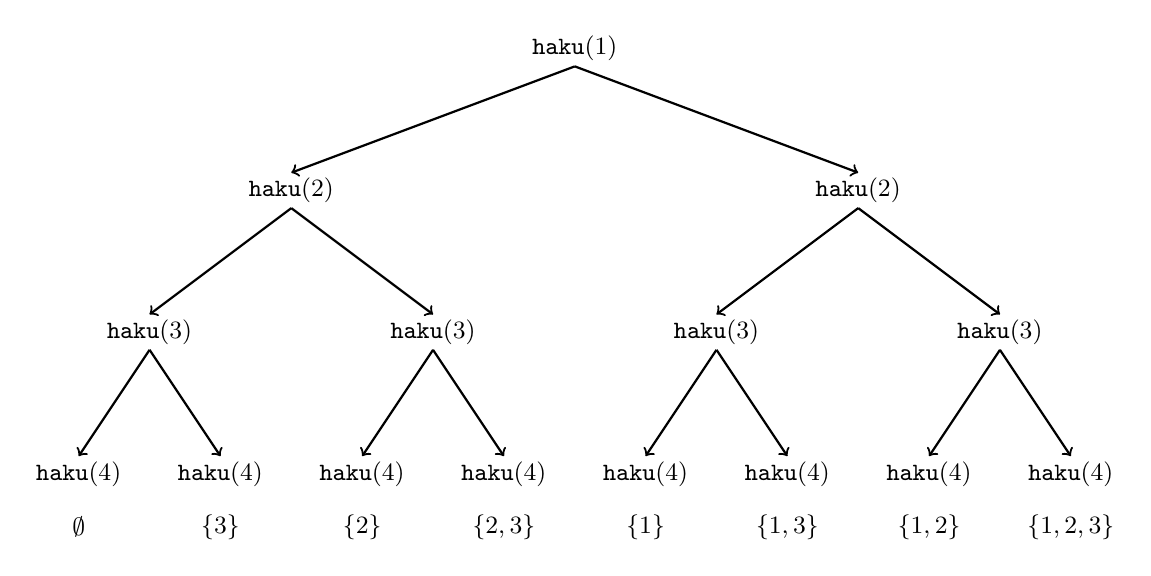
\begin{tikzpicture}[scale=.45]
  \begin{scope}
    \small
    \node at (0,0) {$\texttt{haku}(1)$};

    \node at (-8,-4) {$\texttt{haku}(2)$};
    \node at (8,-4) {$\texttt{haku}(2)$};

    \path[draw,thick,->] (0,0-0.5) -- (-8,-4+0.5);
    \path[draw,thick,->] (0,0-0.5) -- (8,-4+0.5);

    \node at (-12,-8) {$\texttt{haku}(3)$};
    \node at (-4,-8) {$\texttt{haku}(3)$};
    \node at (4,-8) {$\texttt{haku}(3)$};
    \node at (12,-8) {$\texttt{haku}(3)$};

    \path[draw,thick,->] (-8,-4-0.5) -- (-12,-8+0.5);
    \path[draw,thick,->] (-8,-4-0.5) -- (-4,-8+0.5);
    \path[draw,thick,->] (8,-4-0.5) -- (4,-8+0.5);
    \path[draw,thick,->] (8,-4-0.5) -- (12,-8+0.5);

    \node at (-14,-12) {$\texttt{haku}(4)$};
    \node at (-10,-12) {$\texttt{haku}(4)$};
    \node at (-6,-12) {$\texttt{haku}(4)$};
    \node at (-2,-12) {$\texttt{haku}(4)$};
    \node at (2,-12) {$\texttt{haku}(4)$};
    \node at (6,-12) {$\texttt{haku}(4)$};
    \node at (10,-12) {$\texttt{haku}(4)$};
    \node at (14,-12) {$\texttt{haku}(4)$};

    \node at (-14,-13.5) {$\emptyset$};
    \node at (-10,-13.5) {$\{3\}$};
    \node at (-6,-13.5) {$\{2\}$};
    \node at (-2,-13.5) {$\{2,3\}$};
    \node at (2,-13.5) {$\{1\}$};
    \node at (6,-13.5) {$\{1,3\}$};
    \node at (10,-13.5) {$\{1,2\}$};
    \node at (14,-13.5) {$\{1,2,3\}$};


    \path[draw,thick,->] (-12,-8-0.5) -- (-14,-12+0.5);
    \path[draw,thick,->] (-12,-8-0.5) -- (-10,-12+0.5);
    \path[draw,thick,->] (-4,-8-0.5) -- (-6,-12+0.5);
    \path[draw,thick,->] (-4,-8-0.5) -- (-2,-12+0.5);
    \path[draw,thick,->] (4,-8-0.5) -- (2,-12+0.5);
    \path[draw,thick,->] (4,-8-0.5) -- (6,-12+0.5);
    \path[draw,thick,->] (12,-8-0.5) -- (10,-12+0.5);
    \path[draw,thick,->] (12,-8-0.5) -- (14,-12+0.5);
\end{scope}
\end{tikzpicture}
\end{center}

\subsubsection{Menetelmä 2}

Toinen tapa käydä osajoukot läpi on hyödyntää kokonaislukujen
bittiesitystä. Jokainen $n$ alkion osajoukko
voidaan esittää $n$ bitin jonona,
joka taas vastaa lukua väliltä $0 \ldots 2^n-1$.
Bittiesityksen ykkösbitit ilmaisevat,
mitkä joukon alkiot on valittu osajoukkoon.

Tarkastellaan esimerkiksi joukkoa $\{1,2,3,4,5\}$.
Nyt jokaista joukon osajoukkoa vastaa jokin
5 bitin jono.
Esimerkiksi osajoukon $\{2,3,5\}$ bittiesitys on 01101,
jossa bitit 1 ja 4 ovat nollia
ja bitit 2, 3, ja 5 ovat ykkösiä.

Seuraava koodi käy läpi $n$ alkion joukon
osajoukkojen bittiesitykset:

\begin{lstlisting}
for (int b = 0; b < (1<<n); b++) {
    // käsittele osajoukko b
}
\end{lstlisting}

Seuraava koodi muodostaa jokaisen osajoukon
kohdalla vektorin \texttt{v},
joka sisältää osajoukossa olevat luvut.
Ne saadaan selville tutkimalla, mitkä bitit ovat
ykkösiä osajoukon bittiesityksessä.

\begin{lstlisting}
for (int b = 0; b < (1<<n); b++) {
    vector<int> v;
    for (int i = 0; i < n; i++) {
        if (b&(1<<i)) v.push_back(i+1);
    }
}
\end{lstlisting}

\section{Permutaatioiden läpikäynti}

\index{permutaatio}

Joukon permutaatiot ovat alkioiden mahdolliset
järjestykset.
Kun joukossa on $n$ alkiota,
permutaatioita on kaikkiaan $n!$.
Esimerkiksi joukon $\{1,2,3\}$
permutaatiot ovat $(1,2,3)$, $(1,3,2)$,
$(2,1,3)$, $(2,3,1)$, $(3,1,2)$ ja $(3,2,1)$.

\subsubsection{Menetelmä 1}

Osajoukkojen tavoin permutaatioita voi muodostaa
rekursiivisesti.
Seuraava funktio \texttt{haku} käy läpi
joukon $\{1,2,\ldots,n\}$ permutaatiot.
Funktio muodostaa kunkin permutaation
vuorollaan vektoriin \texttt{v}.
Permutaatioiden muodostus alkaa kutsumalla
funktiota ilman parametreja.

\begin{lstlisting}
void haku() {
    if (v.size() == n) {
        // käsittele permutaatio
    } else {
        for (int i = 1; i <= n; i++) {
            if (p[i]) continue;
            p[i] = 1;
            v.push_back(i);
            haku();
            p[i] = 0;
            v.pop_back();
        }
    }
}
\end{lstlisting}

Funktion jokainen kutsu lisää uuden
luvun permutaatioon vektoriin \texttt{v}.
Taulukko \texttt{p} kertoo, mitkä luvut on jo
valittu permutaatioon.
Jos $\texttt{p}[k]=0$, luku $k$ ei ole mukana,
ja jos $\texttt{p}[k]=1$, luku $k$ on mukana.
Jos vektorin \texttt{v} koko on sama kuin
joukon koko $n$, permutaatio on tullut valmiiksi.

\subsubsection{Menetelmä 2}

\index{\texttt{next\_permutation}}

Vaihtoehtoinen tapa käydä läpi permutaatiot
on käyttää C++:n standardikirjastoon kuuluvaa
funktiota \texttt{next\_permutation}.
Se muuttaa taulukossa olevan permutaation
seuraavaksi järjestyksessä olevaksi permutaatioksi.

Seuraava koodi muodostaa joukon $\{1,2,\ldots,n\}$
permutaatiot käyttäen apuna funktiota \texttt{next\_permutation}:

\begin{lstlisting}
vector<int> v;
for (int i = 1; i <= n; i++) {
    v.push_back(i);
}
do {
    // käsittele permutaatio
} while (next_permutation(v.begin(),v.end()));
\end{lstlisting}

\section{Peruuttava haku}

\index{peruuttava haku}

\key{Peruuttava haku}
aloittaa ratkaisun etsimisen tyhjästä
ja laajentaa ratkaisua askel kerrallaan.
Joka askeleella haku haarautuu kaikkiin
mahdollisiin suuntiin, joihin ratkaisua voi laajentaa.
Haaran tutkimisen jälkeen haku peruuttaa takaisin
ja jatkaa muihin mahdollisiin suuntiin.

Tarkastellaan esimerkkinä seuraavaa tehtävää:

\begin{task}
Montako tapaa on asettaa $n$ kuningatarta
$n \times n$ -shakkilaudalle niin,
että mitkään kaksi kuningatarta eivät uhkaa toisiaan?
\end{task}

Esimerkiksi kun $n=4$, mahdolliset ratkaisut ovat seuraavat:

\begin{center}
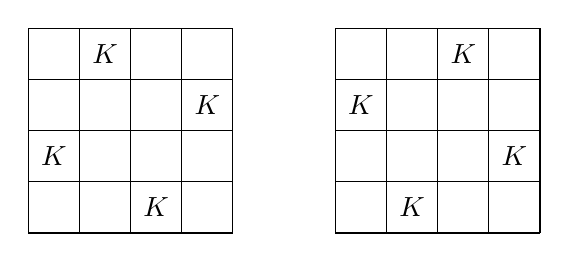
\begin{tikzpicture}[scale=.65]
  \begin{scope}
    \draw (0, 0) grid (4, 4);
    \node at (1.5,3.5) {$K$};
    \node at (3.5,2.5) {$K$};
    \node at (0.5,1.5) {$K$};
    \node at (2.5,0.5) {$K$};

    \draw (6, 0) grid (10, 4);
    \node at (6+2.5,3.5) {$K$};
    \node at (6+0.5,2.5) {$K$};
    \node at (6+3.5,1.5) {$K$};
    \node at (6+1.5,0.5) {$K$};

  \end{scope}
\end{tikzpicture}
\end{center}

Tehtävän voi ratkaista peruuttavalla haulla
muodostamalla ratkaisua rivi kerrallaan.
Jokaisella rivillä täytyy valita yksi ruuduista,
johon sijoitetaan kuningatar niin,
ettei se uhkaa mitään aiemmin lisättyä kuningatarta.
Ratkaisu on valmis, kun viimeisellekin
riville on lisätty kuningatar.

Esimerkiksi kun $n=4$, osa peruuttavan haun muodostamasta
puusta näyttää seuraavalta:

\begin{center}
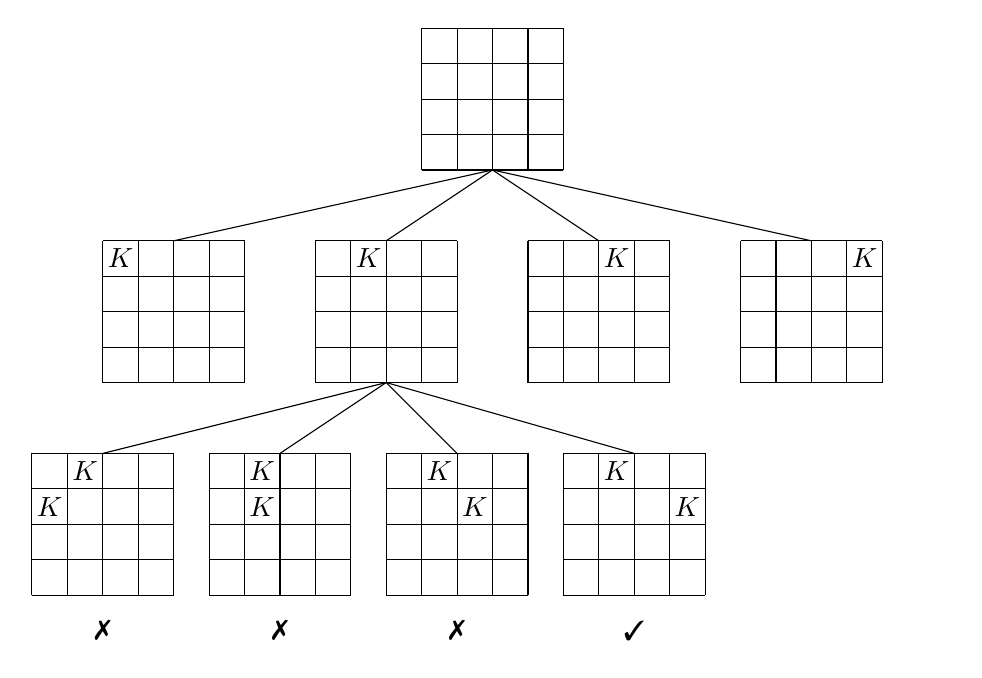
\begin{tikzpicture}[scale=.45]
  \begin{scope}
    \draw (0, 0) grid (4, 4);

    \draw (-9, -6) grid (-5, -2);
    \draw (-3, -6) grid (1, -2);
    \draw (3, -6) grid (7, -2);
    \draw (9, -6) grid (13, -2);

    \node at (-9+0.5,-3+0.5) {$K$};
    \node at (-3+1+0.5,-3+0.5) {$K$};
    \node at (3+2+0.5,-3+0.5) {$K$};
    \node at (9+3+0.5,-3+0.5) {$K$};

    \draw (2,0) -- (-7,-2);
    \draw (2,0) -- (-1,-2);
    \draw (2,0) -- (5,-2);
    \draw (2,0) -- (11,-2);

    \draw (-11, -12) grid (-7, -8);
    \draw (-6, -12) grid (-2, -8);
    \draw (-1, -12) grid (3, -8);
    \draw (4, -12) grid (8, -8);
    \draw[white] (11, -12) grid (15, -8);
    \node at (-11+1+0.5,-9+0.5) {$K$};
    \node at (-6+1+0.5,-9+0.5) {$K$};
    \node at (-1+1+0.5,-9+0.5) {$K$};
    \node at (4+1+0.5,-9+0.5) {$K$};
    \node at (-11+0+0.5,-10+0.5) {$K$};
    \node at (-6+1+0.5,-10+0.5) {$K$};
    \node at (-1+2+0.5,-10+0.5) {$K$};
    \node at (4+3+0.5,-10+0.5) {$K$};

    \draw (-1,-6) -- (-9,-8);
    \draw (-1,-6) -- (-4,-8);
    \draw (-1,-6) -- (1,-8);
    \draw (-1,-6) -- (6,-8);

    \node at (-9,-13) {\ding{55}};
    \node at (-4,-13) {\ding{55}};
    \node at (1,-13) {\ding{55}};
    \node at (6,-13) {\ding{51}};

  \end{scope}
\end{tikzpicture}
\end{center}

Kuvan alimmalla tasolla kolme ensimmäistä osaratkaisua
eivät kelpaa, koska niissä kuningattaret uhkaavat
toisiaan.
Sen sijaan neljäs osaratkaisu kelpaa,
ja sitä on mahdollista laajentaa loppuun asti
kokonaiseksi ratkaisuksi.

\begin{samepage}
Seuraava koodi toteuttaa peruuttavan haun:

\begin{lstlisting}
void haku(int y) {
    if (y == n) {
        c++;
        return;
    }
    for (int x = 0; x < n; x++) {
        if (xx[x] || d1[x+y] || d2[x-y+n-1]) continue;
        xx[x] = d1[x+y] = d2[x-y+n-1] = 1;
        haku(y+1);
        xx[x] = d1[x+y] = d2[x-y+n-1] = 0;
    }
}
\end{lstlisting}
\end{samepage}
Haku alkaa kutsumalla funktiota \texttt{haku(0)}.
Laudan koko on muuttujassa $n$,
ja koodi laskee ratkaisuiden määrän
muuttujaan $c$.

Koodi olettaa, että laudan vaaka- ja pystyrivit
on numeroitu 0:sta alkaen.
Funktio asettaa kuningattaren vaakariville $y$,
kun $0 \le y < n$.
Jos taas $y=n$, yksi ratkaisu on valmis
ja funktio kasvattaa muuttujaa $c$.

Taulukko \texttt{xx} pitää kirjaa,
millä laudan pystyriveillä on jo kuningatar.
Vastaavasti taulukot \texttt{d1} ja \texttt{d2}
pitävät kirjaa vinoriveistä.
Tällaisille riveille ei voi laittaa enää toista
kuningatarta.
Esimerkiksi $4 \times 4$ -laudan tapauksessa
vinorivit on numeroitu seuraavasti:

\begin{center}
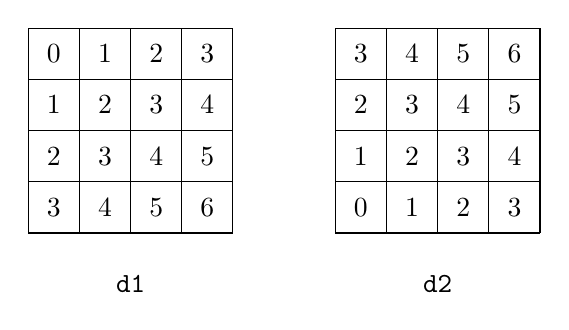
\begin{tikzpicture}[scale=.65]
  \begin{scope}
    \draw (0, 0) grid (4, 4);
    \node at (0.5,3.5) {$0$};
    \node at (1.5,3.5) {$1$};
    \node at (2.5,3.5) {$2$};
    \node at (3.5,3.5) {$3$};
    \node at (0.5,2.5) {$1$};
    \node at (1.5,2.5) {$2$};
    \node at (2.5,2.5) {$3$};
    \node at (3.5,2.5) {$4$};
    \node at (0.5,1.5) {$2$};
    \node at (1.5,1.5) {$3$};
    \node at (2.5,1.5) {$4$};
    \node at (3.5,1.5) {$5$};
    \node at (0.5,0.5) {$3$};
    \node at (1.5,0.5) {$4$};
    \node at (2.5,0.5) {$5$};
    \node at (3.5,0.5) {$6$};

    \draw (6, 0) grid (10, 4);
    \node at (6.5,3.5) {$3$};
    \node at (7.5,3.5) {$4$};
    \node at (8.5,3.5) {$5$};
    \node at (9.5,3.5) {$6$};
    \node at (6.5,2.5) {$2$};
    \node at (7.5,2.5) {$3$};
    \node at (8.5,2.5) {$4$};
    \node at (9.5,2.5) {$5$};
    \node at (6.5,1.5) {$1$};
    \node at (7.5,1.5) {$2$};
    \node at (8.5,1.5) {$3$};
    \node at (9.5,1.5) {$4$};
    \node at (6.5,0.5) {$0$};
    \node at (7.5,0.5) {$1$};
    \node at (8.5,0.5) {$2$};
    \node at (9.5,0.5) {$3$};

    \node at (2,-1) {\texttt{d1}};
    \node at (8,-1) {\texttt{d2}};

  \end{scope}
\end{tikzpicture}
\end{center}

Koodin avulla selviää esimerkiksi,
että tapauksessa $n=8$ on 92 tapaa sijoittaa 8
kuningatarta $8 \times 8$ -laudalle.
Kun $n$ kasvaa, koodi hidastuu nopeasti,
koska ratkaisujen määrä kasvaa räjähdysmäisesti.
Tapauksen $n=16$ laskeminen vie jo noin minuutin
nykyaikaisella tietokoneella (14772512 ratkaisua).

\section{Haun optimointi}

Peruuttavaa hakua on usein mahdollista tehostaa
huomattavasti erilaisten optimointien avulla.
Tarkastellaan esimerkkinä seuraavaa tehtävää:

\begin{task}
Aloitat $n \times n$ -ruudukon
vasemmasta yläkulmasta ja tehtäväsi on päästä
oikeaan alakulmaan.
Saat liikkua joka vuorolla askeleen
ylöspäin, alaspäin, vasemmalle tai oikealle.
Sinun tulee käydä reitin aikana tasan kerran
kussakin ruudussa.
Montako erilaista reittiä on olemassa?
\end{task}

Esimerkiksi $7 \times 7$ -ruudukossa on
111712 mahdollista reittiä vasemmasta yläkulmasta
oikeaan alakulmaan, joista yksi on seuraava:

\begin{center}
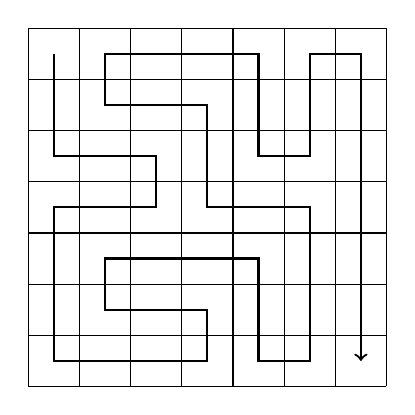
\begin{tikzpicture}[scale=.65]
  \begin{scope}
    \draw (0, 0) grid (7, 7);
    \draw[thick,->] (0.5,6.5) -- (0.5,4.5) -- (2.5,4.5) --
          (2.5,3.5) -- (0.5,3.5) -- (0.5,0.5) --
          (3.5,0.5) -- (3.5,1.5) -- (1.5,1.5) --
          (1.5,2.5) -- (4.5,2.5) -- (4.5,0.5) --
          (5.5,0.5) -- (5.5,3.5) -- (3.5,3.5) --
          (3.5,5.5) -- (1.5,5.5) -- (1.5,6.5) --
          (4.5,6.5) -- (4.5,4.5) -- (5.5,4.5) --
          (5.5,6.5) -- (6.5,6.5) -- (6.5,0.5);
  \end{scope}
\end{tikzpicture}
\end{center}

Keskitymme seuraavaksi nimenomaan tapaukseen $7 \times 7$,
koska se on laskennallisesti sopivan haastava.
Lähdemme liikkeelle suoraviivaisesta peruuttavaa hakua
käyttävästä algoritmista
ja teemme siihen pikkuhiljaa optimointeja,
jotka nopeuttavat hakua eri tavoin.

Mittaamme jokaisen optimoinnin jälkeen
algoritmin suoritusajan sekä rekursiokutsujen yhteismäärän,
jotta näemme selvästi, mikä vaikutus kullakin
optimoinnilla on haun tehokkuuteen.

\subsubsection{Algoritmi}

Algoritmin ensimmäisessä versiossa ei ole mitään optimointeja,
vaan peruuttava haku käy läpi kaikki mahdolliset tavat
muodostaa reitti ruudukon vasemmasta yläkulmasta
oikeaan alakulmaan.

\begin{itemize}
\item
suoritusaika: 483 sekuntia
\item
rekursiokutsuja: 76 miljardia
\end{itemize}

\subsubsection{Optimointi 1}

Reitin ensimmäinen askel on joko alaspäin
tai oikealle. Tästä valinnasta seuraavat tilanteet
ovat symmetrisiä ruudukon lävistäjän suhteen.
Niinpä voimme mennä aina ensin alaspäin
ja kertoa lopuksi reittien määrä 2:lla.

\begin{itemize}
\item
suoritusaika: 244 sekuntia
\item
rekursiokutsuja: 38 miljardia
\end{itemize}

\subsubsection{Optimointi 2}

Jos reitti menee oikean alakulman ruutuun ennen kuin
se on käynyt kaikissa muissa ruuduissa,
siitä ei voi mitenkään enää saada kelvollista ratkaisua.
Niinpä voimme hylätä haun aikana kaikki tällaiset reitit.

\begin{itemize}
\item
suoritusaika: 119 sekuntia
\item
rekursiokutsuja: 20 miljardia
\end{itemize}

\subsubsection{Optimointi 3}

Jos reitti osuu seinään niin, että kummallakin puolella
on ruutu, jossa reitti ei ole vielä käynyt,
ruudukko jakautuu kahteen osaan.
Näin on esimerkiksi seuraavassa tilanteessa:

\begin{center}
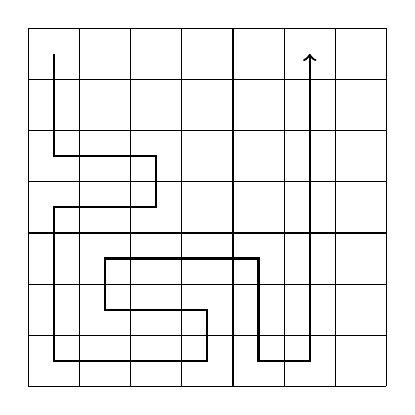
\begin{tikzpicture}[scale=.65]
  \begin{scope}
    \draw (0, 0) grid (7, 7);
    \draw[thick,->] (0.5,6.5) -- (0.5,4.5) -- (2.5,4.5) --
          (2.5,3.5) -- (0.5,3.5) -- (0.5,0.5) --
          (3.5,0.5) -- (3.5,1.5) -- (1.5,1.5) --
          (1.5,2.5) -- (4.5,2.5) -- (4.5,0.5) --
          (5.5,0.5) -- (5.5,6.5);
  \end{scope}
\end{tikzpicture}
\end{center}

Nyt ei ole enää mahdollista käydä kaikissa ruuduissa,
joten voimme hylätä kaikki tällaiset reitit.
Tämä optimointi on hyvin hyödyllinen:

\begin{itemize}
\item
suoritusaika: 1{,}8 sekuntia
\item
rekursiokutsuja: 221 miljoonaa
\end{itemize}

\subsubsection{Optimointi 4}

Äskeisen optimoinnin ideaa voi yleistää:
jos nykyisen ruudun ylä- ja alapuolella on
seinä tai aiemmin käyty ruutu
sekä vasemmalla ja oikealla on
vielä käymätön ruutu (tai päinvastoin),
voimme hylätä reitin.

\begin{itemize}
\item
suoritusaika: 0{,}6 sekuntia
\item
rekursiokutsuja: 69 miljoonaa
\end{itemize}

~\\
Nyt on hyvä hetki lopettaa optimointi ja muistella,
mistä lähdimme liikkeelle.
Alkuperäinen algoritmi vei aikaa 483 sekuntia,
ja nyt optimointien jälkeen algoritmi vie aikaa
vain 0{,}6 sekuntia.
Optimointien ansiosta algoritmin nopeutui
siis lähes 1000-kertaisesti!

Tämä on yleinen ilmiö peruuttavassa haussa,
koska hakupuu on yleensä valtava ja
yksinkertainenkin optimointi voi karsia suuren
määrän haaroja hakupuusta.
Erityisen hyödyllisiä ovat optimoinnit,
jotka kohdistuvat hakupuun yläosaan,
koska ne karsivat eniten haaroja.

\section{Puolivälihaku}

\index{puolivälihaku}

\key{Puolivälihaku} (''meet in the middle'') on tekniikka,
jossa hakutehtävä jaetaan kahteen yhtä suureen osaan.
Kumpaankin osaan tehdään erillinen haku,
ja lopuksi hakujen tulokset yhdistetään.
Puolivälihaun hyötynä on, että sen avulla voi
parantaa haun aikavaativuutta.

\begin{samepage}
Tutustumme puolivälihakuun seuraavan tehtävän kautta:
\begin{task}
Annettuna on lista, jossa on $n$ lukua,
sekä lisäksi kokonaisluku $x$.
Tehtäväsi on selvittää, voiko listan luvuista
valita osajoukon niin, että osajoukon lukujen summa on $x$.
\end{task}
\end{samepage}

Tavanomainen ratkaisu tehtävään on käydä kaikki
listan alkioiden osajoukot läpi ja tarkastaa,
onko jonkin osajoukon summa $x$.
Tällainen ratkaisu kuluttaa aikaa $O(2^n)$,
koska erilaisia osajoukkoja on $2^n$.
Puolivälihaun avulla on kuitenkin mahdollista luoda
tehokkaampi $O(2^{n/2})$-aikainen ratkaisu.

Ideana on jakaa syötteenä oleva lista
kahteen listaan $A$ ja $B$,
joista kumpikin sisältää noin puolet alkioista.
Ensimmäinen haku muodostaa kaikki osajoukot
listan $A$ luvuista ja laittaa muistiin niiden summat
listaan $S_A$.
Toinen haku käsittelee vastaavasti listan $B$ luvut
ja laittaa niiden summat listaan $S_B$.
Tämän jälkeen riittää tarkastaa,
onko mahdollista valita yksi luku listasta $S_A$
ja toinen luku listasta $S_B$ niin,
että lukujen summa on $x$.
Tämän on mahdollista tarkalleen silloin,
kun alkuperäisen listan luvuista saa summan $x$.

Tarkastellaan esimerkkiä,
jossa lista on $\{2,4,5,9\}$
ja $x=15$.
Puolivälihaku muodostaa listat $A=\{2,4\}$
ja $B=\{5,9\}$ sekä summalistat
$S_A=\{0,2,4,6\}$ ja $S_B=\{0,5,9,14\}$.
Summa $x=15$ on mahdollista muodostaa,
koska voidaan valita $S_A$:sta luku $6$
ja $S_B$:stä luku $9$.
Tämä vastaa ratkaisua $\{2,4,9\}$.

Ratkaisun aikavaativuus on huolellisesti toteutettuna
vain $O(2^{n/2})$.
Listat $S_A$ ja $S_B$ on kumpikin mahdollista
muodostaa ajassa $O(2^{n/2})$ niin,
että niiden luvut ovat järjestyksessä.
Tämän jälkeen on mahdollista tutkia ajassa
$O(2^{n/2})$, voiko lukua $x$ muodostaa
valitsemalla kummastakin listasta yksi luku.

Vaikka aikavaativuudet $O(2^n)$ ja $O(2^{n/2})$
muistuttavat toisiaan, niiden ero on merkittävä.
Vakiokertoimilla \emph{on} siis väliä, jos ne esiintyvät
potenssin eksponentissa.
Esimerkiksi jos $n=40$, $O(2^n)$-algoritmin suoritus
veisi tunteja aikaa, kun taas $O(2^{n/2})$
valmistuu sekunnin murto-osassa.

\chapter{Ahneet algoritmit}

\index{ahne algoritmi}

Ahne algoritmi (\textit{greedy algorithm})
muodostaa ongelman ratkaisun
tekemällä joka askeleella
sillä hetkellä parhaalta näyttävän valinnan.
Ahne algoritmi ei koskaan 
peruuta tekemiään valintoja vaan
muodostaa ratkaisun suoraan valmiiksi.
Tämän ansiosta ahneet algoritmit ovat
yleensä hyvin tehokkaita.

Vaikeutena ahneissa algoritmeissa on
keksiä toimiva ahne strategia,
joka tuottaa aina optimaalisen ratkaisun tehtävään.
Ahneen algoritmin tulee olla sellainen,
että kulloinkin parhaalta näyttävät valinnat
tuottavat myös parhaan kokonaisuuden.
Tämän perusteleminen on usein hankalaa.

\section{Kolikkotehtävä}

Aloitamme ahneisiin algoritmeihin tutustumisen
seuraavasta tehtävästä:

\begin{task}
Kolikoiden arvot ovat $\{c_1,c_2,\ldots,c_k\}$,
ja tehtäväsi on muodostaa kolikoista rahamäärä $x$.
Jokaista kolikkoa on saatavilla rajattomasti.
Mikä on pienin määrä kolikoita,
joilla rahamäärän voi muodostaa?
\end{task}

\noindent
Esimerkiksi jos kolikot ovat eurokolikot eli sentteinä
\[\{1,2,5,10,20,50,100,200\}\]
ja muodostettava rahamäärä on 520,
kolikoita tarvitaan vähintään 4.
Optimiratkaisu on valita kolikot $200+200+100+20$.

\subsubsection{Ahne algoritmi}

Luonteva ahne algoritmi tehtävään
on poistaa rahamäärästä aina mahdollisimman
suuri kolikko, kunnes rahamäärä on 0.
Tämä algoritmi toimii esimerkissä,
koska rahamäärästä 520 
poistetaan ensin kahdesti 200, sitten 100
ja lopuksi 20.
Mutta toimiiko ahne algoritmi aina oikein?

Osoittautuu, että eurokolikoiden tapauksessa
ahne algoritmi toimii aina oikein,
eli se tuottaa aina ratkaisun,
jossa on pienin määrä kolikoita.
Algoritmin toimivuuden voi perustella
seuraavasti:

Kutakin kolikkoa 1, 5, 10, 50 ja 100
on optimiratkaisussa enintään yksi.
Tämä johtuu siitä, että jos
ratkaisussa olisi kaksi tällaista kolikkoa,
saman ratkaisun voisi muodostaa
käyttäen vähemmän kolikoita.
Esimerkiksi jos ratkaisussa on
kolikot $5+5$, ne voi korvata kolikolla 10.

Vastaavasti kumpaakin kolikkoa 2 ja 20
on optimiratkaisussa enintään kaksi,
koska kolikot $2+2+2$ voi korvata kolikoilla $1+5$
ja kolikot $20+20+20$ voi korvata kolikoilla $10+50$.
Lisäksi ratkaisussa ei voi olla yhdistelmiä
$1+2+2$ ja $10+20+20$,
koska ne voi korvata kolikoilla 5 ja 50.

Näiden havaintojen perusteella
jokaiselle kolikolle $x$ pätee,
että $x$:ää pienemmistä kolikoista
ei ole mahdollista saada aikaan summaa
$x$ tai suurempaa summaa optimaalisesti.
Esimerkiksi jos $x=100$, pienemmistä kolikoista
saa korkeintaan summan $50+20+20+5+2+2=99$.
Niinpä ahne algoritmi,
joka valitsee aina suurimman kolikon,
tuottaa optimiratkaisun.

Kuten tästä esimerkistä huomaa,
ahneen algoritmin toimivuuden perusteleminen
voi olla vaikeaa,
vaikka kyseessä olisi yksinkertainen algoritmi.

\subsubsection{Yleinen tapaus}

Yleisessä tapauksessa kolikot voivat olla mitä tahansa.
Tällöin suurimman kolikon valitseva ahne algoritmi
ei välttämättä tuota optimiratkaisua.

Jos ahne algoritmi ei toimi, tämän voi osoittaa
näyttämällä vastaesimerkin, jossa algoritmi
antaa väärän vastauksen.
Tässä tehtävässä vastaesimerkki on helppoa keksiä:
jos kolikot ovat $\{1,3,4\}$ ja muodostettava
rahamäärä on 6, ahne algoritmi tuottaa ratkaisun
$1+1+4$, kun taas optimiratkaisu on $3+3$.

Yleisessä tapauksessa tehtävän ratkaisuun
ei tunneta ahnetta algoritmia,
mutta palaamme tehtävään seuraavassa luvussa.
Tehtävään on nimittäin olemassa dynaamista
ohjelmointia käyttävä algoritmi,
joka tuottaa optimiratkaisun
millä tahansa kolikoilla ja rahamäärällä.

\section{Aikataulutus}

Monet aikataulutukseen liittyvät ongelmat
ratkeavat ahneilla algoritmeilla.
Tällaisissa ongelmissa on monta luontevaa
ahnetta ratkaisua, mutta useimmat niistä
eivät tuota aina optimiratkaisua.
Tutustumme seuraavaksi kahteen
klassiseen aikataulutusongelmaan.

\subsection{Tapahtumien valinta}

\begin{task}
Annettuna on $n$ tapahtumaa,
jotka alkavat ja päättyvät tiettyinä hetkinä.
Tehtäväsi on suunnitella aikataulu,
jota seuraamalla pystyt osallistumaan
mahdollisimman moneen tapahtumaan.
Et voi osallistua tapahtumaan vain osittain.
\end{task}

\newpage
Esimerkiksi jos tapahtumat ovat

\begin{center}
\begin{tabular}{lll}
tapahtuma & alkuaika & loppuaika \\
\hline
$A$ & 1 & 3 \\
$B$ & 2 & 5 \\
$C$ & 3 & 9 \\
$D$ & 6 & 8 \\
\end{tabular}
\end{center}

\noindent
niin on mahdollista osallistua korkeintaan
kahteen tapahtumaan.
Yksi mahdollisuus on osallistua tapahtumiin
$B$ ja $D$ seuraavasti:
\\
\begin{center}
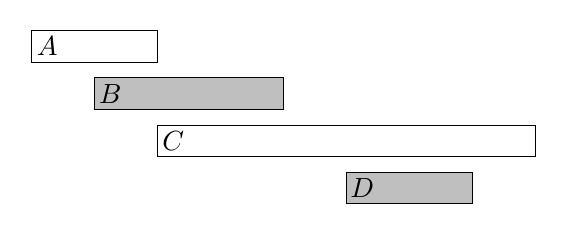
\begin{tikzpicture}[scale=.4]
  \begin{scope}
    \draw (2, 0) rectangle (6, -1);
    \draw[fill=lightgray] (4, -1.5) rectangle (10, -2.5);
    \draw (6, -3) rectangle (18, -4);
    \draw[fill=lightgray] (12, -4.5) rectangle (16, -5.5);
    \node at (2.5,-0.5) {$A$};
    \node at (4.5,-2) {$B$};
    \node at (6.5,-3.5) {$C$};
    \node at (12.5,-5) {$D$};
  \end{scope}
\end{tikzpicture}
\end{center}

\noindent
Tehtävän ratkaisuun on mahdollista 
keksiä useita ahneita algoritmeja,
mutta mikä niistä toimii kaikissa tapauksissa?

\subsubsection*{Algoritmi 1}

Ensimmäinen idea on valita ratkaisuun
mahdollisimman lyhyitä tapahtumia.
Esimerkin tapauksessa tällainen
algoritmi valitsee tapahtumat
\\
\begin{center}
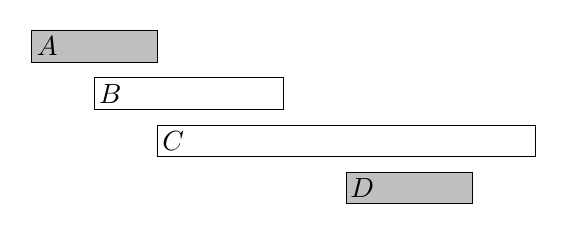
\begin{tikzpicture}[scale=.4]
  \begin{scope}
    \draw[fill=lightgray] (2, 0) rectangle (6, -1);
    \draw (4, -1.5) rectangle (10, -2.5);
    \draw (6, -3) rectangle (18, -4);
    \draw[fill=lightgray] (12, -4.5) rectangle (16, -5.5);
    \node at (2.5,-0.5) {$A$};
    \node at (4.5,-2) {$B$};
    \node at (6.5,-3.5) {$C$};
    \node at (12.5,-5) {$D$};
  \end{scope}
\end{tikzpicture}
\end{center}
ja tuottaa optimiratkaisun.

Lyhimpien tapahtumien valinta ei ole kuitenkaan
aina toimiva strategia.
Algoritmi epäonnistuu esimerkiksi seuraavassa tilanteessa:
\\
\begin{center}
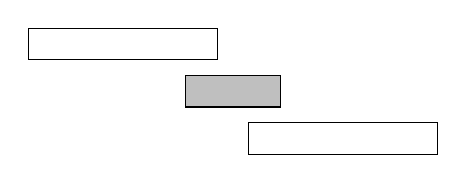
\begin{tikzpicture}[scale=.4]
  \begin{scope}
    \draw (1, 0) rectangle (7, -1);
    \draw[fill=lightgray] (6, -1.5) rectangle (9, -2.5);
    \draw (8, -3) rectangle (14, -4);
  \end{scope}
\end{tikzpicture}
\end{center}

Kun lyhyt tapahtuma valitaan mukaan,
on mahdollista osallistua vain yhteen tapahtumaan.
Kuitenkin valitsemalla pitkät tapahtumat
olisi mahdollista osallistua kahteen tapahtumaan.

\subsubsection*{Algoritmi 2}

Toinen idea on valita aina seuraavaksi tapahtuma,
joka alkaa mahdollisimman aikaisin.
Tämä algoritmi valitsee esimerkissä tapahtumat
\\
\begin{center}
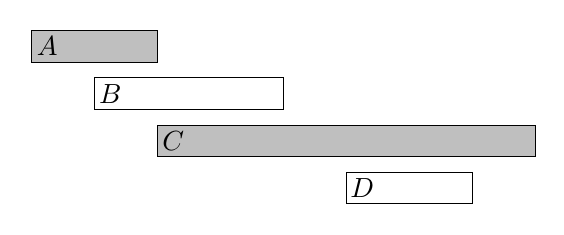
\begin{tikzpicture}[scale=.4]
  \begin{scope}
    \draw[fill=lightgray] (2, 0) rectangle (6, -1);
    \draw (4, -1.5) rectangle (10, -2.5);
    \draw[fill=lightgray] (6, -3) rectangle (18, -4);
    \draw (12, -4.5) rectangle (16, -5.5);
    \node at (2.5,-0.5) {$A$};
    \node at (4.5,-2) {$B$};
    \node at (6.5,-3.5) {$C$};
    \node at (12.5,-5) {$D$};
  \end{scope}
\end{tikzpicture}
\end{center}
ja tuottaa optimiratkaisun.

Tämä algoritmi ei kuitenkaan toimi
esimerkiksi seuraavassa tilanteessa:
\\
\begin{center}
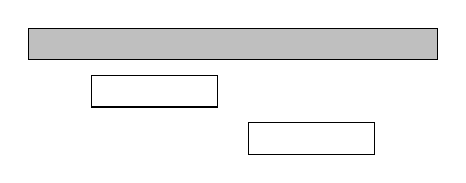
\begin{tikzpicture}[scale=.4]
  \begin{scope}
    \draw[fill=lightgray] (1, 0) rectangle (14, -1);
    \draw (3, -1.5) rectangle (7, -2.5);
    \draw (8, -3) rectangle (12, -4);
  \end{scope}
\end{tikzpicture}
\end{center}

Kun ensimmäisenä alkava tapahtuma
valitaan mukaan, mitään muuta tapahtumaa
ei ole mahdollista valita.
Kuitenkin olisi mahdollista osallistua
kahteen tapahtumaan valitsemalla
kaksi myöhempää tapahtumaa.

\subsubsection*{Algoritmi 3}

Kolmas idea on valita aina seuraavaksi tapahtuma,
joka päättyy mahdollisimman aikaisin.
Tämä algoritmi valitsee esimerkissä tapahtumat
\\
\begin{center}
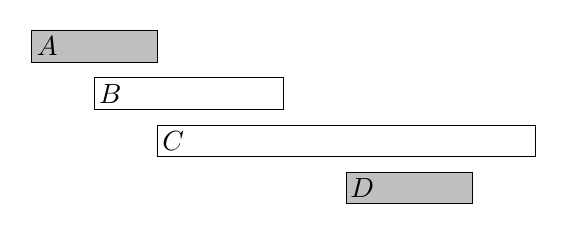
\begin{tikzpicture}[scale=.4]
  \begin{scope}
    \draw[fill=lightgray] (2, 0) rectangle (6, -1);
    \draw (4, -1.5) rectangle (10, -2.5);
    \draw (6, -3) rectangle (18, -4);
    \draw[fill=lightgray] (12, -4.5) rectangle (16, -5.5);
    \node at (2.5,-0.5) {$A$};
    \node at (4.5,-2) {$B$};
    \node at (6.5,-3.5) {$C$};
    \node at (12.5,-5) {$D$};
  \end{scope}
\end{tikzpicture}
\end{center}
ja tuottaa optimiratkaisun.

Osoittautuu, että tämä ahne algoritmi
tuottaa \textit{aina} optimiratkaisun.
Algoritmi toimii, koska on aina kokonaisuuden
kannalta optimaalista valita
ensimmäiseksi tapahtumaksi
mahdollisimman aikaisin päättyvä tapahtuma.
Tämän jälkeen on taas optimaalista
valita seuraava aikatauluun sopiva
mahdollisimman aikaisin
päättyvä tapahtua, jne.

Yksi tapa perustella valintaa on miettiä,
mitä tapahtuu, jos ensimmäiseksi tapahtumaksi
valitaan jokin muu kuin mahdollisimman
aikaisin päättyvä tapahtuma.
Tällainen valinta ei ole koskaan parempi,
koska myöhemmin päättyvän tapahtuman
jälkeen on joko yhtä paljon tai vähemmän
mahdollisuuksia valita seuraavia tapahtumia.

\subsection{Tehtävien järjestys}

\begin{task}
Annettuna on $n$ tehtävää,
joista jokaisella on kesto ja deadline.
Tehtäväsi on valita järjestys,
jossa suoritat tehtävät.
Saat kustakin tehtävästä $d-x$ pistettä,
missä $d$ on tehtävän deadline ja $x$
on tehtävän valmistumishetki.
Mikä on suurin mahdollinen pistesumma?
\end{task}

Esimerkiksi jos tehtävät ovat

\begin{center}
\begin{tabular}{lll}
tehtävä & kesto & deadline \\
\hline
$A$ & 4 & 2 \\
$B$ & 3 & 5 \\
$C$ & 2 & 7 \\
$D$ & 4 & 5 \\
\end{tabular}
\end{center}

\noindent
niin optimaalinen ratkaisu on suorittaa
tehtävät seuraavasti:

\begin{center}
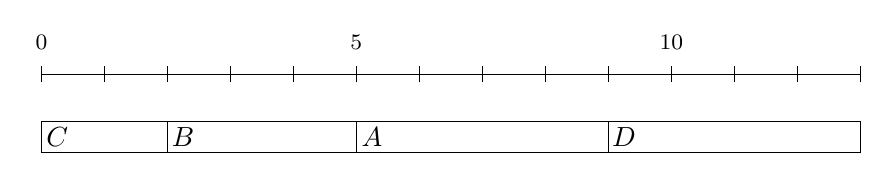
\begin{tikzpicture}[scale=.4]
  \begin{scope}
    \draw (0, 0) rectangle (4, -1);
    \draw (4, 0) rectangle (10, -1);
    \draw (10, 0) rectangle (18, -1);
    \draw (18, 0) rectangle (26, -1);
    \node at (0.5,-0.5) {$C$};
    \node at (4.5,-0.5) {$B$};
    \node at (10.5,-0.5) {$A$};
    \node at (18.5,-0.5) {$D$};

    \draw (0,1.5) -- (26,1.5);
    \foreach \i in {0,2,...,26}
    {
        \draw (\i,1.25) -- (\i,1.75);
    }
    \footnotesize
    \node at (0,2.5) {0};
    \node at (10,2.5) {5};
    \node at (20,2.5) {10};

  \end{scope}
\end{tikzpicture}
\end{center}

Tässä ratkaisussa $C$ tuottaa 5 pistettä,
$B$ tuottaa 0 pistettä, $A$ tuottaa $-7$ pistettä
ja $D$ tuottaa $-8$ pistettä,
joten pistesumma on $-10$.

Yllättävää kyllä, tehtävän optimaalinen ratkaisu
ei riipu lainkaan deadlineista.
Toimiva ahne strategia on
suorittaa tehtävät järjestyksessä keston mukaan
lyhimmästä pisimpään.
Syynä tähän on, että jos missä tahansa vaiheessa
suoritetaan peräkkäin kaksi tehtävää,
joista ensimmäinen kestää toista kauemmin,
tehtävien järjestyksen vaihtaminen parantaa ratkaisua.

Esimerkiksi jos peräkkäin ovat tehtävät

\begin{center}
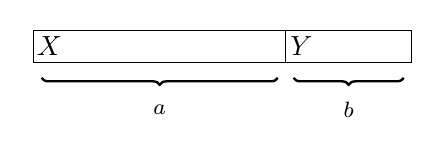
\begin{tikzpicture}[scale=.4]
  \begin{scope}
    \draw (0, 0) rectangle (8, -1);
    \draw (8, 0) rectangle (12, -1);
    \node at (0.5,-0.5) {$X$};
    \node at (8.5,-0.5) {$Y$};

\draw [decoration={brace}, decorate, line width=0.3mm] (7.75,-1.5) -- (0.25,-1.5);
\draw [decoration={brace}, decorate, line width=0.3mm] (11.75,-1.5) -- (8.25,-1.5);

\footnotesize
\node at (4,-2.5) {$a$};
\node at (10,-2.5) {$b$};

  \end{scope}
\end{tikzpicture}
\end{center}

ja $a>b$, niin järjestyksen muuttaminen muotoon

\begin{center}
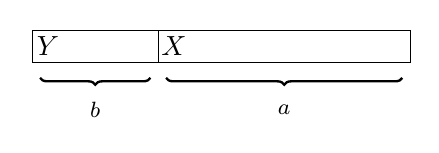
\begin{tikzpicture}[scale=.4]
  \begin{scope}
    \draw (0, 0) rectangle (4, -1);
    \draw (4, 0) rectangle (12, -1);
    \node at (0.5,-0.5) {$Y$};
    \node at (4.5,-0.5) {$X$};

\draw [decoration={brace}, decorate, line width=0.3mm] (3.75,-1.5) -- (0.25,-1.5);
\draw [decoration={brace}, decorate, line width=0.3mm] (11.75,-1.5) -- (4.25,-1.5);

\footnotesize
\node at (2,-2.5) {$b$};
\node at (8,-2.5) {$a$};

  \end{scope}
\end{tikzpicture}
\end{center}

antaa $X$:lle $b$ pistettä vähemmän ja $Y$:lle $a$ pistettä enemmän,
joten kokonaismuutos pistemäärään on $a-b > 0$.
Optimiratkaisussa
kaikille peräkkäin suoritettaville tehtäville
tulee päteä, että lyhyempi tulee ennen pidempää,
mistä seuraa, että tehtävät tulee suorittaa
järjestyksessä keston mukaan.

\section{Keskiluvut}

\subsection{Itseisarvosumma}

\begin{task}
Annettuna on $n$ lukua $a_1,a_2,\ldots,a_n$.
Tehtäväsi on etsiä luku $x$, joka minimoi summan
$|a_1-x|+|a_2-x|+\cdots+|a_n-x|.$
\end{task}

Esimerkiksi jos luvut ovat $[1,2,9,2,6]$,
niin paras ratkaisu on $x=2$,
jolloin summaksi tulee
\[
|1-2|+|2-2|+|9-2|+|2-2|+|6-2|=12.
\]

Yleisessä tapauksessa paras valinta $x$:n arvoksi
on lukujen \textit{mediaani}
eli keskimmäinen luku järjestyksessä.
Esimerkiksi luvut $[1,2,9,2,6]$
ovat järjestyksessä $[1,2,2,6,9]$,
joten mediaani on 2.

Mediaanin valinta on paras ratkaisu,
koska jos $x$ on mediaania pienempi,
$x$:n suurentaminen pienentää summaa.
Vastaavasti jos $x$ on mediaania suurempi,
$x$:n pienentäminen pienentää summaa.
Niinpä $x$ kannattaa siirtää mahdollisimman
lähelle mediaania eli optimiratkaisu on
valita $x$ mediaaniksi.

Jos $n$ on parillinen ja mediaaneja on kaksi,
kumpikin mediaani sekä kaikki niiden välillä
olevat luvut tuottavat optimaalisen ratkaisun.

\subsection{Neliösumma}

\begin{task}
Annettuna on $n$ lukua $a_1,a_2,\ldots,a_n$.
Tehtäväsi on etsiä luku $x$, joka minimoi summan
$(a_1-x)^2+(a_2-x)^2+\cdots+(a_n-x)^2.$
\end{task}

Esimerkiksi jos luvut ovat $[1,2,9,2,6]$,
niin paras ratkaisu on $x=4$,
jolloin summaksi tulee
\[
(1-4)^2+(2-4)^2+(9-4)^2+(2-4)^2+(6-4)^2=46.
\]

\noindent
Nyt yleisessä tapauksessa
paras valinta $x$:n arvoksi on lukujen
\textit{keskiarvo}.
Esimerkissä lukujen keskiarvo on $(1+2+9+2+6)/5=4$.

Tämän tuloksen voi johtaa järjestämällä summan
uudestaan muotoon

\[
(a_1^2+a_2^2+\cdots+a_n^2)-2x(a_1+a_2+\cdots+a_n)+nx^2.
\]

Ensimmäinen osa ei riipu $x$:stä, joten sen voi jättää huomiotta.
Jäljelle jäävistä osista muodostuu funktio
$nx^2-2xs$, missä $s=a_1+a_2+\cdots+a_n$.
Tämä on ylöspäin aukeava paraabeli,
jonka nollakohdat ovat $x=0$ ja $x=2s/n$
ja pienin arvo on näiden keskikohta
$x=s/n$ eli taulukon lukujen keskiarvo.


\chapter{Dynaaminen ohjelmointi}

\index{dynaaminen ohjelmointi@dynaaminen ohjelmointi}

\key{Dynaaminen ohjelmointi}
on tekniikka, joka yhdistää täydellisen haun
toimivuuden ja ahneiden algoritmien tehokkuuden.
Dynaamisen ohjelmoinnin käyttäminen edellyttää,
että tehtävä jakautuu osaongelmiin,
jotka voidaan käsitellä toisistaan riippumattomasti.

Dynaamisella ohjelmoinnilla on kaksi käyttötarkoitusta:

\begin{itemize}
\item
\key{Optimiratkaisun etsiminen}:
Haluamme etsiä ratkaisun, joka on
jollakin tavalla suurin mahdollinen
tai pienin mahdollinen.
\item
\key{Ratkaisuiden määrän laskeminen}:
Haluamme laskea, kuinka monta mahdollista
ratkaisua on olemassa.
\end{itemize}

Tutustumme dynaamiseen ohjelmointiin ensin
optimiratkaisun etsimisen kautta ja käytämme sitten
samaa ideaa ratkaisujen määrän laskemiseen.

Dynaamisen ohjelmoinnin ymmärtäminen on yksi merkkipaalu
jokaisen kisakoodarin uralla.
Vaikka menetelmän perusidea on yksinkertainen,
haasteena on oppia soveltamaan sitä sujuvasti
erilaisissa tehtävissä.
Tämä luku esittelee joukon
perusesimerkkejä, joista on hyvä lähteä liikkeelle.

\section{Kolikkotehtävä}

Aloitamme dynaamisen ohjelmoinnin tutun tehtävän kautta:
Muodostettavana on rahamäärä $x$
käyttäen mahdollisimman vähän kolikoita.
Kolikoiden arvot ovat $\{c_1,c_2,\ldots,c_k\}$
ja jokaista kolikkoa on saatavilla rajattomasti.

Luvussa 6.1 ratkaisimme tehtävän ahneella algoritmilla,
joka muodostaa rahamäärän valiten mahdollisimman
suuria kolikoita.
Ahne algoritmi toimii esimerkiksi silloin,
kun kolikot ovat eurokolikot,
mutta yleisessä tapauksessa ahne algoritmi
ei välttämättä valitse pienintä määrää kolikoita.

Nyt on aika ratkaista tehtävä tehokkaasti
dynaamisella ohjelmoinnilla niin,
että algoritmi toimii millä tahansa kolikoilla.
Ratkaisu perustuu rekursiiviseen funktioon,
joka käy läpi kaikki vaihtoehdot rahamäärän
muodostamiseen täydellisen haun kaltaisesti.
Ratkaisu toimii kuitenkin tehokkaasti, koska
se tallentaa välituloksia muistitaulukkoon,
minkä ansiosta sen ei tarvitse laskea samoja
asioita moneen kertaan.

\subsubsection{Rekursiivinen esitys}

\index{rekursioyhtxlz@rekursioyhtälö}

Dynaamisessa ohjelmoinnissa on ideana esittää
ongelma rekursiivisesti niin,
että ongelman ratkaisun voi laskea
saman ongelman pienempien tapausten ratkaisuista.
Tässä tehtävässä luonteva ongelma on seuraava:
mikä on pienin määrä kolikoita,
joilla voi muodostaa rahamäärän $x$?

Merkitään $f(x)$ funktiota,
joka antaa vastauksen ongelmaan,
eli $f(x)$ on pienin määrä kolikoita,
joilla voi muodostaa rahamäärän $x$.
Funktion arvot riippuvat siitä,
mitkä kolikot ovat käytössä.
Esimerkiksi jos kolikot ovat $\{1,3,4\}$,
funktion ensimmäiset arvot ovat:

\[
\begin{array}{lcl}
f(0) & = & 0 \\
f(1) & = & 1 \\
f(2) & = & 2 \\
f(3) & = & 1 \\
f(4) & = & 1 \\
f(5) & = & 2 \\
f(6) & = & 2 \\
f(7) & = & 2 \\
f(8) & = & 2 \\
f(9) & = & 3 \\
f(10) & = & 3 \\
\end{array}
\]

Nyt $f(0)=0$, koska jos rahamäärä on 0,
ei tarvita yhtään kolikkoa.
Vastaavasti $f(3)=1$, koska rahamäärän 3
voi muodostaa kolikolla 3,
ja $f(5)=2$, koska rahamäärän 5
voi muodostaa kolikoilla 1 ja 4.

Oleellinen ominaisuus funktiossa on,
että arvon $f(x)$ pystyy laskemaan
rekursiivisesti käyttäen pienempiä
funktion arvoja.
Esimerkiksi jos kolikot ovat $\{1,3,4\}$,
on kolme tapaa alkaa muodostaa rahamäärää $x$:
valitaan kolikko 1, 3 tai 4.
Jos valitaan kolikko 1, täytyy
muodostaa vielä rahamäärä $x-1$.
Vastaavasti jos valitaan kolikko 3 tai 4,
täytyy muodostaa rahamäärä $x-3$ tai $x-4$.

Niinpä rekursiivinen kaava on
\[f(x) = \min(f(x-1),f(x-3),f(x-4))+1,\]
missä funktio $\min$ valitsee pienimmän parametreistaan.
Yleisemmin jos kolikot ovat $\{c_1,c_2,\ldots,c_k\}$,
rekursiivinen kaava on
\[f(x) = \min(f(x-c_1),f(x-c_2),\ldots,f(x-c_k))+1.\]
Funktion pohjatapauksena on
\[f(0)=0,\]
koska rahamäärän 0 muodostamiseen ei tarvita
yhtään kolikkoa.
Lisäksi on hyvä määritellä
\[f(x)=\infty,\hspace{8px}\textrm{jos $x<0$}.\]
Tämä tarkoittaa, että negatiivisen rahamäärän
muodostaminen vaatii äärettömästi kolikoita,
mikä estää sen, että rekursio muodostaisi
ratkaisun, johon kuuluu negatiivinen rahamäärä.

Nyt voimme toteuttaa funktion C++:lla suoraan
rekursiivisen määritelmän perusteella:

\begin{lstlisting}
int f(int x) {
    if (x == 0) return 0;
    if (x < 0) return 1e9;
    int u = 1e9;
    for (int i = 1; i <= k; i++) {
        u = min(u, f(x-c[i])+1);
    }
    return u;
}
\end{lstlisting}

Koodi olettaa, että käytettävät kolikot ovat
$\texttt{c}[1], \texttt{c}[2], \ldots, \texttt{c}[n]$,
ja arvo $10^9$ kuvastaa ääretöntä.
Tämä on toimiva funktio, mutta se ei ole vielä tehokas,
koska funktio käy läpi valtavasti erilaisia tapoja
muodostaa rahamäärä.
Seuraavaksi esiteltävä muistitaulukko tekee
funktiosta tehokkaan.

\subsubsection{Muistitaulukko}

\index{muistitaulukko@muistitaulukko}

Dynaaminen ohjelmointi tehostaa
rekursiivisen funktion laskentaa
tallentamalla funktion arvoja \key{muistitaulukkoon}.
Taulukon avulla funktion arvo
tietyllä parametrilla riittää laskea
vain kerran, minkä jälkeen sen voi
hakea suoraan taulukosta.
Tämä muutos nopeuttaa algoritmia ratkaisevasti.

Tässä tehtävässä muistitaulukoksi sopii taulukko

\begin{lstlisting}
int d[N];
\end{lstlisting}

jonka kohtaan $\texttt{d}[x]$
lasketaan funktion arvo $f(x)$.
Vakio $N$ valitaan niin, että kaikki
laskettavat funktion arvot mahtuvat taulukkoon.

Tämän jälkeen funktion voi toteuttaa
tehokkaasti näin:

\begin{lstlisting}
int f(int x) {
    if (x == 0) return 0;
    if (x < 0) return 1e9;
    if (d[x]) return d[x];
    int u = 1e9;
    for (int i = 1; i <= k; i++) {
        u = min(u, f(x-c[i])+1);
    }
    d[x] = u;
    return d[x];
}
\end{lstlisting}

Funktio käsittelee pohjatapaukset $x=0$
ja $x<0$ kuten ennenkin.
Sitten funktio tarkastaa,
onko $f(x)$ laskettu jo taulukkoon $\texttt{d}[x]$.
Jos $f(x)$ on laskettu,
funktio palauttaa sen suoraan.
Muussa tapauksessa funktio laskee arvon rekursiivisesti
ja tallentaa sen kohtaan $\texttt{d}[x]$.

Muistitaulukon ansiosta funktio toimii
nopeasti, koska sen tarvitsee laskea
vastaus kullekin $x$:n arvolle
vain kerran rekursiivisesti.
Heti kun arvo $f(x)$ on tallennettu muistitaulukkoon,
sen saa haettua sieltä suoraan,
kun funktiota kutsutaan seuraavan kerran parametrilla $x$.

Tuloksena olevan algoritmin aikavaativuus on $O(xk)$,
kun rahamäärä on $x$ ja kolikoiden määrä on $k$.
Käytännössä ratkaisu on mahdollista toteuttaa,
jos $x$ on niin pieni, että on mahdollista varata 
riittävän suuri muistitaulukko.

Huomaa, että muistitaulukon voi muodostaa
myös suoraan silmukalla ilman rekursiota
laskemalla arvot pienimmästä suurimpaan:
\begin{lstlisting}
d[0] = 0;
for (int i = 1; i <= x; i++) {
    int u = 1e9;
    for (int j = 1; j <= k; j++) {
        if (i-c[j] < 0) continue;
        u = min(u, d[i-c[j]]+1);
    }
    d[i] = u;
}
\end{lstlisting}

Silmukkatoteutus on lyhyempi ja
hieman tehokkaampi kuin rekursiototeutus,
minkä vuoksi kokeneet kisakoodarit
toteuttavat dynaamisen ohjelmoinnin
usein silmukan avulla.
Kuitenkin silmukkatoteutuksen taustalla
on sama rekursiivinen idea kuin ennenkin.

\subsubsection{Ratkaisun muodostaminen}

Joskus optimiratkaisun arvon selvittämisen lisäksi
täytyy muodostaa näytteeksi yksi mahdollinen optimiratkaisu.
Tässä tehtävässä tämä tarkoittaa,
että ohjelman täytyy antaa esimerkki
tavasta valita kolikot,
joista muodostuu rahamäärä $x$
käyttäen mahdollisimman vähän kolikoita.

Ratkaisun muodostaminen onnistuu lisäämällä
koodiin uuden taulukon, joka kertoo
kullekin rahamäärälle,
mikä kolikko siitä tulee poistaa
optimiratkaisussa.
Seuraavassa koodissa taulukko \texttt{e}
huolehtii asiasta:

\begin{lstlisting}
d[0] = 0;
for (int i = 1; i <= x; i++) {
    d[i] = 1e9;
    for (int j = 1; j <= k; j++) {
        if (i-c[j] < 0) continue;
        int u = d[i-c[j]]+1;
        if (u < d[i]) {
            d[i] = u;
            e[i] = c[j];
        }
    }
}
\end{lstlisting}

Tämän jälkeen rahamäärän $x$ muodostavat
kolikot voi tulostaa näin:

\begin{lstlisting}
while (x > 0) {
    cout << e[x] << "\n";
    x -= e[x];
}
\end{lstlisting}

\subsubsection{Ratkaisuiden määrän laskeminen}

Tarkastellaan sitten kolikkotehtävän muunnelmaa,
joka on muuten samanlainen kuin ennenkin,
mutta laskettavana on mahdollisten ratkaisuiden yhteismäärä
optimaalisen ratkaisun sijasta.
Esimerkiksi jos kolikot ovat $\{1,3,4\}$ ja rahamäärä on 5,
niin ratkaisuja on kaikkiaan 6:

\begin{multicols}{2}
\begin{itemize}
\item $1+1+1+1+1$
\item $1+1+3$
\item $1+3+1$
\item $3+1+1$
\item $1+4$
\item $4+1$
\end{itemize}
\end{multicols}

Ratkaisujen määrän laskeminen tapahtuu melko samalla tavalla
kuin optimiratkaisun etsiminen.
Erona on, että optimiratkaisun etsivässä rekursiossa
valitaan yleensä pienin tai suurin aiempi arvo,
kun taas ratkaisujen määrän laskevassa rekursiossa lasketaan
yhteen kaikki vaihtoehdot.

Tässä tapauksessa voimme muodostaa funktion $f(x)$,
joka kertoo, monellako tavalla rahamäärän $x$
voi muodostaa kolikoista.
Esimerkiksi $f(5)=6$, kun kolikot ovat $\{1,3,4\}$.
Funktion $f(x)$ saa laskettua rekursiivisesti kaavalla
\[ f(x) = f(x-c_1)+f(x-c_2)+\cdots+f(x-c_k),\]
koska rahamäärän $x$ muodostamiseksi pitää
valita jokin kolikko $c_i$ ja muodostaa sen jälkeen rahamäärä $x-c_i$.
Pohjatapauksina ovat $f(0)=1$, koska rahamäärä 0 syntyy
ilman yhtään kolikkoa,
sekä $f(x)=0$, kun $x<0$, koska negatiivista rahamäärää
ei ole mahdollista muodostaa.
Yllä olevassa esimerkissä funktioksi tulee
\[ f(x) = f(x-1)+f(x-3)+f(x-4) \]
ja funktion ensimmäiset arvot ovat:
\[
\begin{array}{lcl}
f(0) & = & 1 \\
f(1) & = & 1 \\
f(2) & = & 1 \\
f(3) & = & 2 \\
f(4) & = & 4 \\
f(5) & = & 6 \\
f(6) & = & 9 \\
f(7) & = & 15 \\
f(8) & = & 25 \\
f(9) & = & 40 \\
\end{array}
\]

Seuraava koodi laskee funktion $f(x)$ arvon
dynaamisella ohjelmoinnilla täyttämällä taulukon
\texttt{d} rahamäärille $0 \ldots x$:

\begin{lstlisting}
d[0] = 1;
for (int i = 1; i <= x; i++) {
    for (int j = 1; j <= k; j++) {
        if (i-c[j] < 0) continue;
        d[i] += d[i-c[j]];
    }
}
\end{lstlisting}

Usein ratkaisujen määrä on niin suuri, että sitä ei tarvitse
laskea kokonaan vaan riittää ilmoittaa vastaus
modulo $m$, missä esimerkiksi $m=10^9+7$.
Tämä onnistuu muokkaamalla koodia niin,
että kaikki laskutoimitukset lasketaan modulo $m$.
Tässä tapauksessa riittää lisätä rivin
\begin{lstlisting}
        d[i] += d[i-c[j]];
\end{lstlisting}
jälkeen rivi
\begin{lstlisting}
        d[i] %= m;
\end{lstlisting}

Nyt olemme käyneet läpi kaikki dynaamisen
ohjelmoinnin perusasiat.
Dynaamista ohjelmointia voi soveltaa monilla
tavoilla erilaisissa tehtävissä,
minkä vuoksi tutustumme seuraavaksi
joukkoon tehtäviä, jotka esittelevät
dynaamisen ohjelmoinnin mahdollisuuksia.

\section{Pisin nouseva alijono}

\index{pisin nouseva alijono@pisin nouseva alijono}

Annettuna on taulukko, jossa on $n$
kokonaislukua $x_1,x_2,\ldots,x_n$.
Tehtävänä on selvittää,
kuinka pitkä on taulukon
\key{pisin nouseva alijono}
eli vasemmalta oikealle kulkeva
ketju taulukon alkioita,
jotka on valittu niin,
että jokainen alkio on edellistä suurempi.
Esimerkiksi taulukossa

\begin{center}
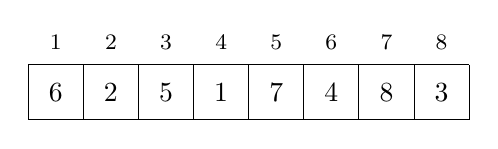
\begin{tikzpicture}[scale=0.7]
\draw (0,0) grid (8,1);
\node at (0.5,0.5) {$6$};
\node at (1.5,0.5) {$2$};
\node at (2.5,0.5) {$5$};
\node at (3.5,0.5) {$1$};
\node at (4.5,0.5) {$7$};
\node at (5.5,0.5) {$4$};
\node at (6.5,0.5) {$8$};
\node at (7.5,0.5) {$3$};

\footnotesize
\node at (0.5,1.4) {$1$};
\node at (1.5,1.4) {$2$};
\node at (2.5,1.4) {$3$};
\node at (3.5,1.4) {$4$};
\node at (4.5,1.4) {$5$};
\node at (5.5,1.4) {$6$};
\node at (6.5,1.4) {$7$};
\node at (7.5,1.4) {$8$};
\end{tikzpicture}
\end{center}
pisin nouseva alijono sisältää 4 lukua:
\begin{center}
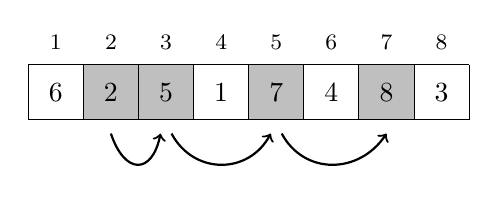
\begin{tikzpicture}[scale=0.7]
\fill[color=lightgray] (1,0) rectangle (2,1);
\fill[color=lightgray] (2,0) rectangle (3,1);
\fill[color=lightgray] (4,0) rectangle (5,1);
\fill[color=lightgray] (6,0) rectangle (7,1);
\draw (0,0) grid (8,1);
\node at (0.5,0.5) {$6$};
\node at (1.5,0.5) {$2$};
\node at (2.5,0.5) {$5$};
\node at (3.5,0.5) {$1$};
\node at (4.5,0.5) {$7$};
\node at (5.5,0.5) {$4$};
\node at (6.5,0.5) {$8$};
\node at (7.5,0.5) {$3$};

\draw[thick,->] (1.5,-0.25) .. controls (1.75,-1.00) and (2.25,-1.00) .. (2.4,-0.25);
\draw[thick,->] (2.6,-0.25) .. controls (3.0,-1.00) and (4.0,-1.00) .. (4.4,-0.25);
\draw[thick,->] (4.6,-0.25) .. controls (5.0,-1.00) and (6.0,-1.00) .. (6.5,-0.25);

\footnotesize
\node at (0.5,1.4) {$1$};
\node at (1.5,1.4) {$2$};
\node at (2.5,1.4) {$3$};
\node at (3.5,1.4) {$4$};
\node at (4.5,1.4) {$5$};
\node at (5.5,1.4) {$6$};
\node at (6.5,1.4) {$7$};
\node at (7.5,1.4) {$8$};
\end{tikzpicture}
\end{center}

Merkitään $f(k)$ kohtaan $k$ päättyvän
pisimmän nousevan alijonon pituutta,
jolloin ratkaisu tehtävään on suurin
arvoista $f(1),f(2),\ldots,f(n)$.
Esimerkiksi yllä olevassa taulukossa
funktion arvot ovat seuraavat:
\[
\begin{array}{lcl}
f(1) & = & 1 \\
f(2) & = & 1 \\
f(3) & = & 2 \\
f(4) & = & 1 \\
f(5) & = & 3 \\
f(6) & = & 2 \\
f(7) & = & 4 \\
f(8) & = & 2 \\
\end{array}
\]

Arvon $f(k)$ laskemisessa on kaksi vaihtoehtoa,
millainen kohtaan $k$ päättyvä pisin nouseva alijono on:
\begin{enumerate}
\item Pisin nouseva alijono sisältää vain luvun $x_k$,
jolloin $f(k)=1$.
\item Valitaan jokin kohta $i$, jolle pätee $i<k$
ja $x_i<x_k$.
Pisin nouseva alijono saadaan liittämällä
kohtaan $i$ päättyvän pisimmän nousevan alijonon perään luku $x_k$.
Tällöin $f(k)=f(i)+1$.
\end{enumerate}

Tarkastellaan esimerkkinä arvon $f(7)$ laskemista.
Paras ratkaisu on ottaa pohjaksi kohtaan 5
päättyvä pisin nouseva alijono $[2,5,7]$
ja lisätä sen perään luku $x_7=8$.
Tuloksena on alijono $[2,5,7,8]$ ja $f(7)=f(5)+1=4$.

Suoraviivainen tapa toteuttaa algoritmi on
käydä kussakin kohdassa $k$ läpi kaikki kohdat
$i=1,2,\ldots,k-1$, joissa voi olla alijonon
edellinen luku.
Tällaisen algoritmin aikavaativuus on $O(n^2)$.
Yllättävää kyllä, algoritmin voi toteuttaa myös
ajassa $O(n \log n)$, mutta tämä on vaikeampaa.

\section{Reitinhaku ruudukossa}

Seuraava tehtävämme on etsiä reitti
$n \times n$ -ruudukon vasemmasta yläkulmasta
oikeaan alakulmaan.
Jokaisessa ruudussa on luku, ja reitti
tulee muodostaa niin, että reittiin kuuluvien
lukujen summa on mahdollisimman suuri.
Rajoituksena ruudukossa on mahdollista
liikkua vain oikealla ja alaspäin.

Seuraavassa ruudukossa paras reitti
on merkitty harmaalla taustalla:
\begin{center}
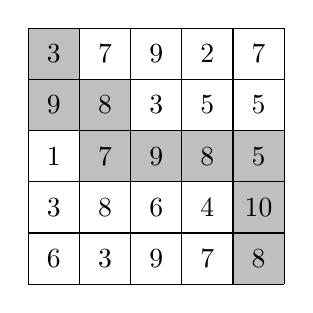
\begin{tikzpicture}[scale=.65]
  \begin{scope}
    \fill [color=lightgray] (0, 9) rectangle (1, 8);
    \fill [color=lightgray] (0, 8) rectangle (1, 7);
    \fill [color=lightgray] (1, 8) rectangle (2, 7);
    \fill [color=lightgray] (1, 7) rectangle (2, 6);
    \fill [color=lightgray] (2, 7) rectangle (3, 6);
    \fill [color=lightgray] (3, 7) rectangle (4, 6);
    \fill [color=lightgray] (4, 7) rectangle (5, 6);
    \fill [color=lightgray] (4, 6) rectangle (5, 5);
    \fill [color=lightgray] (4, 5) rectangle (5, 4);
    \draw (0, 4) grid (5, 9);
    \node at (0.5,8.5) {3};
    \node at (1.5,8.5) {7};
    \node at (2.5,8.5) {9};
    \node at (3.5,8.5) {2};
    \node at (4.5,8.5) {7};
    \node at (0.5,7.5) {9};
    \node at (1.5,7.5) {8};
    \node at (2.5,7.5) {3};
    \node at (3.5,7.5) {5};
    \node at (4.5,7.5) {5};
    \node at (0.5,6.5) {1};
    \node at (1.5,6.5) {7};
    \node at (2.5,6.5) {9};
    \node at (3.5,6.5) {8};
    \node at (4.5,6.5) {5};
    \node at (0.5,5.5) {3};
    \node at (1.5,5.5) {8};
    \node at (2.5,5.5) {6};
    \node at (3.5,5.5) {4};
    \node at (4.5,5.5) {10};
    \node at (0.5,4.5) {6};
    \node at (1.5,4.5) {3};
    \node at (2.5,4.5) {9};
    \node at (3.5,4.5) {7};
    \node at (4.5,4.5) {8};
  \end{scope}
\end{tikzpicture}
\end{center}
Tällä reitillä lukujen summa on $3+9+8+7+9+8+5+10+8=67$,
joka on suurin mahdollinen summa vasemmasta yläkulmasta
oikeaan alakulmaan.

Hyvä lähestymistapa tehtävään on laskea
kuhunkin ruutuun $(y,x)$ suurin summa
reitillä vasemmasta yläkulmasta kyseiseen ruutuun.
Merkitään tätä suurinta summaa $f(y,x)$,
jolloin $f(n,n)$ on suurin summa
reitillä vasemmasta yläkulmasta oikeaan alakulmaan.

Rekursio syntyy havainnosta,
että ruutuun $(y,x)$ saapuvan reitin
täytyy tulla joko vasemmalta ruudusta $(y,x-1)$
tai ylhäältä ruudusta $(y-1,x)$:
\begin{center}
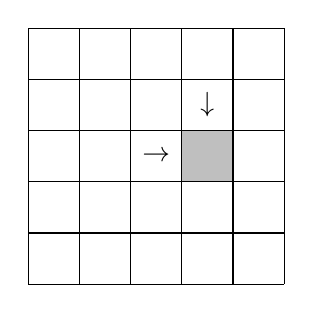
\begin{tikzpicture}[scale=.65]
  \begin{scope}
    \fill [color=lightgray] (3, 7) rectangle (4, 6);
    \draw (0, 4) grid (5, 9);
    
    \node at (2.5,6.5) {$\rightarrow$};
    \node at (3.5,7.5) {$\downarrow$};
    
  \end{scope}
\end{tikzpicture}
\end{center}

Kun $r(y,x)$
on ruudukon luku kohdassa $(y,x)$,
rekursion pohjatapaukset ovat seuraavat:

\[
\begin{array}{lcl}
f(1,1) & = & r(1,1) \\
f(1,x) & = & f(1,x-1)+r(1,x) \\
f(y,1) & = & f(y-1,1)+r(y,1)\\
\end{array}
\]

Yleisessä tapauksessa valittavana on
kaksi reittiä,
joista kannattaa valita se,
joka tuottaa suuremman summan:
\[ f(y,x) = \max(f(y,x-1),f(y-1,x))+r(y,x)\]

Ratkaisun aikavaativuus on $O(n^2)$, koska jokaisessa
ruudussa $f(y,x)$ saadaan laskettua vakioajassa
viereisten ruutujen arvoista.

\section{Repunpakkaus}

\index{repunpakkaus@repunpakkaus}

\key{Repunpakkaus} on klassinen ongelma,
jossa annettuna on $n$ tavaraa,
joiden painot ovat
$p_1,p_2,\ldots,p_n$ ja arvot ovat
$a_1,a_2,\ldots,a_n$.
Tehtävänä on valita reppuun pakattavat tavarat
niin, että tavaroiden
painojen summa on enintään $x$
ja tavaroiden arvojen summa on mahdollisimman suuri.

\begin{samepage}
Esimerkiksi jos tavarat ovat
\begin{center}
\begin{tabular}{rrr}
tavara & paino & arvo \\
\hline
A & 5 & 1 \\
B & 6 & 3 \\
C & 8 & 5 \\
D & 5 & 3 \\
\end{tabular}
\end{center}
\end{samepage}
ja suurin sallittu yhteispaino on 12,
niin paras ratkaisu on pakata reppuun tavarat $B$ ja $D$.
Niiden yhteispaino $6+5=11$ ei ylitä rajaa 12
ja arvojen summa
on $3+3=6$, mikä on paras mahdollinen tulos.

Tämä tehtävä on mahdollista ratkaista kahdella eri
tavalla dynaamisella ohjelmoinnilla
riippuen siitä, tarkastellaanko ongelmaa
maksimointina vai minimointina.
Käymme seuraavaksi läpi molemmat ratkaisut.

\subsubsection{Ratkaisu 1}

\textit{Maksimointi:} Merkitään $f(k,u)$
suurinta mahdollista tavaroiden yhteisarvoa,
kun reppuun pakataan jokin osajoukko
tavaroista $1 \ldots k$,
jossa tavaroiden yhteispaino on $u$.
Ratkaisu tehtävään on suurin arvo
$f(n,u)$, kun $0 \le u \le x$.
Rekursiivinen kaava funktion laskemiseksi on
\[f(k,u) = \max(f(k-1,u),f(k-1,u-p_k)+a_k),\]
koska kohdassa $k$ oleva tavara joko otetaan tai ei oteta
mukaan ratkaisuun.
Pohjatapauksina on $f(0,0)=0$ ja $f(0,u)=-\infty$,
kun $u \neq 0$. Tämän ratkaisun aikavaativuus on $O(nx)$.

Esimerkin tilanteessa optimiratkaisu on
$f(4,11)=6$, joka muodostuu seuraavan ketjun kautta:
\[f(4,11)=f(3,6)+3=f(2,6)+3=f(1,0)+3+3=f(0,0)+3+3=6.\]

\subsubsection{Ratkaisu 2}

\textit{Minimointi:} Merkitään $f(k,u)$
pienintä mahdollista tavaroiden yhteispainoa,
kun reppuun pakataan jokin osajoukko
tavaroista $1 \ldots k$,
jossa tavaroiden yhteisarvo on $u$.
Ratkaisu tehtävään on suurin arvo $u$,
jolle pätee $0 \le u \le s$ ja $f(n,u) \le x$,
missä $s=\sum_{i=1}^n a_i$.
Rekursiivinen kaava funktion laskemiseksi on
\[f(k,u) = \min(f(k-1,u),f(k-1,u-a_k)+p_k)\]
ratkaisua 1 vastaavasti.
Pohjatapauksina on $f(0,0)=0$ ja $f(0,u)=\infty$, kun $u \neq 0$.
Tämän ratkaisun aikavaativuus on $O(ns)$.

Esimerkin tilanteessa optimiratkaisu on
$f(4,6)=11$, joka muodostuu seuraavan ketjun kautta:
\[f(4,6)=f(3,3)+5=f(2,3)+5=f(1,0)+6+5=f(0,0)+6+5=11.\]

~\\
Kiinnostava seikka on, että eri asiat syötteessä
vaikuttavat ratkaisuiden tehokkuuteen.
Ratkaisussa 1 tavaroiden painot vaikuttavat tehokkuuteen
mutta arvoilla ei ole merkitystä.
Ratkaisussa 2 puolestaan tavaroiden arvot vaikuttavat
tehokkuuteen mutta painoilla ei ole merkitystä.

\section{Editointietäisyys}

\index{editointietxisyys@editointietäisyys}
\index{Levenšteinin etäisyys}

\key{Editointietäisyys} eli
\key{Levenšteinin etäisyys}
kuvaa, kuinka kaukana kaksi merkkijonoa ovat toisistaan.
Se on pienin määrä editointioperaatioita,
joilla ensimmäisen merkkijonon saa muutettua toiseksi.
Sallitut operaatiot ovat:
\begin{itemize}
\item merkin lisäys (esim. \texttt{ABC} $\rightarrow$ \texttt{ABCA})
\item merkin poisto (esim. \texttt{ABC} $\rightarrow$ \texttt{AC})
\item merkin muutos (esim. \texttt{ABC} $\rightarrow$ \texttt{ADC})
\end{itemize}

Esimerkiksi merkkijonojen \texttt{TALO} ja \texttt{PALLO}
editointietäisyys on 2, koska voi tehdä ensin
operaation \texttt{TALO} $\rightarrow$ \texttt{TALLO}
(merkin lisäys) ja sen jälkeen operaation
\texttt{TALLO} $\rightarrow$ \texttt{PALLO}
(merkin muutos).
Tämä on pienin mahdollinen määrä operaatioita, koska
selvästikään yksi operaatio ei riitä.

Oletetaan, että annettuna on merkkijonot
\texttt{x} (pituus $n$ merkkiä) ja
\texttt{y} (pituus $m$ merkkiä),
ja haluamme laskea niiden editointietäisyyden.
Tämä onnistuu tehokkaasti dynaamisella
ohjelmoinnilla ajassa $O(nm)$.
Merkitään funktiolla $f(a,b)$
editointietäisyyttä \texttt{x}:n $a$
ensimmäisen merkin sekä
\texttt{y}:n $b$:n ensimmäisen merkin välillä.
Tämän funktion avulla saa sekä
laskettua tehokkaasti editointietäisyyden että
selvitettyä, mitkä ovat tarvittavat editointioperaatiot.

Funktion pohjatapaukset ovat
\[
\begin{array}{lcl}
f(0,b) & = & b \\
f(a,0) & = & a \\
\end{array}
\]
ja yleisessä tapauksessa pätee kaava
\[ f(a,b) = \min(f(a,b-1)+1,f(a-1,b)+1,f(a-1,b-1)+c),\]
missä $c=0$, jos \texttt{x}:n merkki $a$
ja \texttt{y}:n merkki $b$ ovat samat,
ja muussa tapauksessa $c=1$.
Kaava käy läpi mahdollisuudet lyhentää merkkijonoja:
\begin{itemize}
\item $f(a,b-1)$ tarkoittaa, että $x$:ään lisätään merkki
\item $f(a-1,b)$ tarkoittaa, että $x$:stä poistetaan merkki
\item $f(a-1,b-1)$ tarkoittaa, että $x$:ssä ja $y$:ssä on
sama merkki ($c=0$) tai $x$:n merkki muutetaan $y$:n merkiksi ($c=1$)
\end{itemize}
Seuraava taulukko sisältää funktion $f$ arvot
esimerkin tapauksessa:
\begin{center}
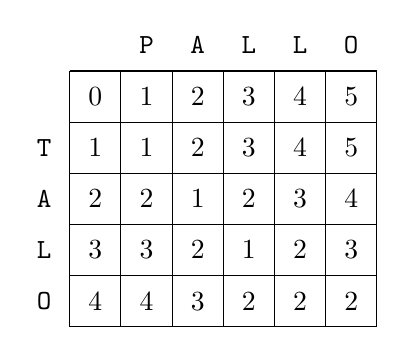
\begin{tikzpicture}[scale=.65]
  \begin{scope}
    %\fill [color=lightgray] (5, -3) rectangle (6, -4);
    \draw (1, -1) grid (7, -6);
    
    \node at (0.5,-2.5) {\texttt{T}};
    \node at (0.5,-3.5) {\texttt{A}};
    \node at (0.5,-4.5) {\texttt{L}};
    \node at (0.5,-5.5) {\texttt{O}};

    \node at (2.5,-0.5) {\texttt{P}};
    \node at (3.5,-0.5) {\texttt{A}};
    \node at (4.5,-0.5) {\texttt{L}};
    \node at (5.5,-0.5) {\texttt{L}};
    \node at (6.5,-0.5) {\texttt{O}};

    \node at (1.5,-1.5) {$0$};
    \node at (1.5,-2.5) {$1$};
    \node at (1.5,-3.5) {$2$};
    \node at (1.5,-4.5) {$3$};
    \node at (1.5,-5.5) {$4$};
    \node at (2.5,-1.5) {$1$};
    \node at (2.5,-2.5) {$1$};
    \node at (2.5,-3.5) {$2$};
    \node at (2.5,-4.5) {$3$};
    \node at (2.5,-5.5) {$4$};
    \node at (3.5,-1.5) {$2$};
    \node at (3.5,-2.5) {$2$};
    \node at (3.5,-3.5) {$1$};
    \node at (3.5,-4.5) {$2$};
    \node at (3.5,-5.5) {$3$};
    \node at (4.5,-1.5) {$3$};
    \node at (4.5,-2.5) {$3$};
    \node at (4.5,-3.5) {$2$};
    \node at (4.5,-4.5) {$1$};
    \node at (4.5,-5.5) {$2$};
    \node at (5.5,-1.5) {$4$};
    \node at (5.5,-2.5) {$4$};
    \node at (5.5,-3.5) {$3$};
    \node at (5.5,-4.5) {$2$};
    \node at (5.5,-5.5) {$2$};
    \node at (6.5,-1.5) {$5$};
    \node at (6.5,-2.5) {$5$};
    \node at (6.5,-3.5) {$4$};
    \node at (6.5,-4.5) {$3$};
    \node at (6.5,-5.5) {$2$};
  \end{scope}
\end{tikzpicture}
\end{center}

Taulukon oikean alanurkan ruutu
kertoo, että merkkijonojen \texttt{TALO}
ja \texttt{PALLO} editointietäisyys on 2.
Taulukosta pystyy myös
lukemaan, miten pienimmän editointietäisyyden
voi saavuttaa.
Tässä tapauksessa polku on seuraava:

\begin{center}
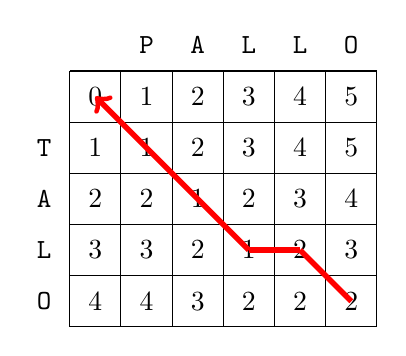
\begin{tikzpicture}[scale=.65]
  \begin{scope}
    \draw (1, -1) grid (7, -6);
    
    \node at (0.5,-2.5) {\texttt{T}};
    \node at (0.5,-3.5) {\texttt{A}};
    \node at (0.5,-4.5) {\texttt{L}};
    \node at (0.5,-5.5) {\texttt{O}};

    \node at (2.5,-0.5) {\texttt{P}};
    \node at (3.5,-0.5) {\texttt{A}};
    \node at (4.5,-0.5) {\texttt{L}};
    \node at (5.5,-0.5) {\texttt{L}};
    \node at (6.5,-0.5) {\texttt{O}};

    \node at (1.5,-1.5) {$0$};
    \node at (1.5,-2.5) {$1$};
    \node at (1.5,-3.5) {$2$};
    \node at (1.5,-4.5) {$3$};
    \node at (1.5,-5.5) {$4$};
    \node at (2.5,-1.5) {$1$};
    \node at (2.5,-2.5) {$1$};
    \node at (2.5,-3.5) {$2$};
    \node at (2.5,-4.5) {$3$};
    \node at (2.5,-5.5) {$4$};
    \node at (3.5,-1.5) {$2$};
    \node at (3.5,-2.5) {$2$};
    \node at (3.5,-3.5) {$1$};
    \node at (3.5,-4.5) {$2$};
    \node at (3.5,-5.5) {$3$};
    \node at (4.5,-1.5) {$3$};
    \node at (4.5,-2.5) {$3$};
    \node at (4.5,-3.5) {$2$};
    \node at (4.5,-4.5) {$1$};
    \node at (4.5,-5.5) {$2$};
    \node at (5.5,-1.5) {$4$};
    \node at (5.5,-2.5) {$4$};
    \node at (5.5,-3.5) {$3$};
    \node at (5.5,-4.5) {$2$};
    \node at (5.5,-5.5) {$2$};
    \node at (6.5,-1.5) {$5$};
    \node at (6.5,-2.5) {$5$};
    \node at (6.5,-3.5) {$4$};
    \node at (6.5,-4.5) {$3$};
    \node at (6.5,-5.5) {$2$};

    \path[draw=red,thick,-,line width=2pt] (6.5,-5.5) -- (5.5,-4.5);
    \path[draw=red,thick,-,line width=2pt] (5.5,-4.5) -- (4.5,-4.5);
    \path[draw=red,thick,->,line width=2pt] (4.5,-4.5) -- (1.5,-1.5);
  \end{scope}
\end{tikzpicture}
\end{center}

Merkkijonojen \texttt{PALLO} ja \texttt{TALO} viimeinen merkki on sama,
joten niiden editointietäisyys on sama kuin
merkkijonojen \texttt{PALL} ja \texttt{TAL}.
Nyt voidaan poistaa viimeinen \texttt{L} merkkijonosta \texttt{PAL},
mistä tulee yksi operaatio.
Editointietäisyys on siis yhden suurempi
kuin merkkijonoilla \texttt{PAL} ja \texttt{TAL}, jne.

\section{Laatoitukset}

Joskus dynaamisen ohjelmoinnin tila on monimutkaisempi kuin
kiinteä yhdistelmä lukuja.
Tarkastelemme lopuksi tehtävää, jossa
laskettavana on, monellako tavalla
kokoa $1 \times 2$ ja $2 \times 1$ olevilla laatoilla
voi täyttää $n \times m$ -kokoisen ruudukon.
Esimerkiksi ruudukolle kokoa $4 \times 7$
yksi mahdollinen ratkaisu on
\begin{center}
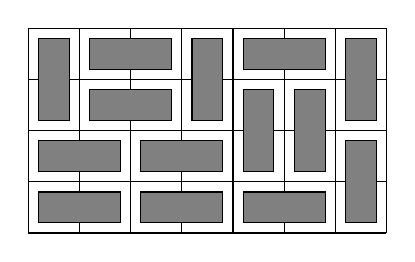
\begin{tikzpicture}[scale=.65]
    \draw (0,0) grid (7,4);
    \draw[fill=gray] (0+0.2,0+0.2) rectangle (2-0.2,1-0.2);
    \draw[fill=gray] (2+0.2,0+0.2) rectangle (4-0.2,1-0.2);
    \draw[fill=gray] (4+0.2,0+0.2) rectangle (6-0.2,1-0.2);
    \draw[fill=gray] (0+0.2,1+0.2) rectangle (2-0.2,2-0.2);
    \draw[fill=gray] (2+0.2,1+0.2) rectangle (4-0.2,2-0.2);
    \draw[fill=gray] (1+0.2,2+0.2) rectangle (3-0.2,3-0.2);
    \draw[fill=gray] (1+0.2,3+0.2) rectangle (3-0.2,4-0.2);
    \draw[fill=gray] (4+0.2,3+0.2) rectangle (6-0.2,4-0.2);

    \draw[fill=gray] (0+0.2,2+0.2) rectangle (1-0.2,4-0.2);
    \draw[fill=gray] (3+0.2,2+0.2) rectangle (4-0.2,4-0.2);
    \draw[fill=gray] (6+0.2,2+0.2) rectangle (7-0.2,4-0.2);
    \draw[fill=gray] (4+0.2,1+0.2) rectangle (5-0.2,3-0.2);
    \draw[fill=gray] (5+0.2,1+0.2) rectangle (6-0.2,3-0.2);
    \draw[fill=gray] (6+0.2,0+0.2) rectangle (7-0.2,2-0.2);

\end{tikzpicture}
\end{center}
ja ratkaisujen yhteismäärä on 781.

Tehtävän voi ratkaista dynaamisella ohjelmoinnilla
käymällä ruudukkoa läpi rivi riviltä.
Jokainen ratkaisun rivi pelkistyy merkkijonoksi,
jossa on $m$ merkkiä joukosta $\{\sqcap, \sqcup, \sqsubset, \sqsupset \}$.
Esimerkiksi yllä olevassa ratkaisussa on 4 riviä,
jotka vastaavat merkkijonoja
\begin{itemize}
\item
$\sqcap \sqsubset \sqsupset \sqcap \sqsubset \sqsupset \sqcap$,
\item
$\sqcup \sqsubset \sqsupset \sqcup \sqcap \sqcap \sqcup$,
\item
$\sqsubset \sqsupset \sqsubset \sqsupset \sqcup \sqcup \sqcap$ ja
\item
$\sqsubset \sqsupset \sqsubset \sqsupset \sqsubset \sqsupset \sqcup$.
\end{itemize}

Tehtävään sopiva rekursiivinen funktio on $f(k,x)$,
joka laskee, montako tapaa on muodostaa ratkaisu
ruudukon riveille $1 \ldots k$ niin,
että riviä $k$ vastaa merkkijono $x$.
Dynaaminen ohjelmointi on mahdollista,
koska jokaisen rivin sisältöä
rajoittaa vain edellisen rivin sisältö.

Riveistä muodostuva ratkaisu on kelvollinen,
jos rivillä 1 ei ole merkkiä $\sqcup$,
rivillä $n$ ei ole merkkiä $\sqcap$
ja kaikki peräkkäiset rivit ovat \emph{yhteensopivat}.
Esimerkiksi rivit
$\sqcup \sqsubset \sqsupset \sqcup \sqcap \sqcap \sqcup$ ja
$\sqsubset \sqsupset \sqsubset \sqsupset \sqcup \sqcup \sqcap$ 
ovat yhteensopivat,
kun taas rivit
$\sqcap \sqsubset \sqsupset \sqcap \sqsubset \sqsupset \sqcap$ ja
$\sqsubset \sqsupset \sqsubset \sqsupset \sqsubset \sqsupset \sqcup$
eivät ole yhteensopivat.

Koska rivillä on $m$ merkkiä ja jokaiselle merkille on 4
vaihtoehtoa, erilaisia rivejä on korkeintaan $4^m$.
Niinpä ratkaisun aikavaativuus on $O(n 4^{2m})$,
koska joka rivillä käydään läpi $O(4^m)$
vaihtoehtoa rivin sisällölle
ja jokaista vaihtoehtoa kohden on $O(4^m)$
vaihtoehtoa edellisen rivin sisällölle.
Käytännössä ruudukko kannattaa kääntää niin
päin, että pienempi sivun pituus on $m$:n roolissa,
koska $m$:n suuruus on ratkaiseva ajankäytön kannalta.

Ratkaisua on mahdollista tehostaa parantamalla rivien esitystapaa merkkijonoina.
Osoittautuu, että ainoa seuraavalla rivillä tarvittava tieto on,
missä kohdissa riviltä lähtee laattoja alaspäin.
Niinpä rivin voikin tallentaa käyttämällä vain merkkejä
$\sqcap$ ja $\Box$, missä $\Box$ kokoaa yhteen vanhat merkit
$\sqcup$, $\sqsubset$ ja $\sqsupset$.
Tällöin erilaisia rivejä on vain $2^m$
ja aikavaativuudeksi tulee $O(n 2^{2m})$.

Mainittakoon lopuksi, että laatoitusten määrän laskemiseen
on myös yllättävä suora kaava
\[ \prod_{a=1}^{\lceil n/2 \rceil} \prod_{b=1}^{\lceil m/2 \rceil} 4 \cdot (\cos^2 \frac{\pi a}{n + 1} + \cos^2 \frac{\pi b}{m+1}).\]
Tämä kaava on sinänsä hyvin tehokas,
koska se laskee laatoitusten määrän ajassa $O(nm)$,
mutta käytännön ongelma kaavan käyttämisessä
on, kuinka tallentaa välitulokset riittävän tarkkoina lukuina.



\chapter{Tasoitettu analyysi}

\index{tasoitettu analyysi@tasoitettu analyysi}

Monen algoritmin aikavaativuuden pystyy laskemaan
suoraan katsomalla algoritmin rakennetta:
mitä silmukoita algoritmissa on ja miten monta
kertaa niitä suoritetaan.
Joskus kuitenkaan näin suoraviivainen analyysi ei
riitä antamaan todellista kuvaa algoritmin tehokkuudesta.

\key{Tasoitettu analyysi} soveltuu sellaisten
algoritmien analyysiin, joiden osana on jokin operaatio,
jonka ajankäyttö vaihtelee.
Ideana on tarkastella yksittäisen operaation
sijasta kaikkia operaatioita algoritmin
aikana ja laskea niiden ajankäytölle yhteinen raja.

\section{Kahden osoittimen tekniikka}

\index{kahden osoittimen tekniikka}

\key{Kahden osoittimen tekniikka} on taulukon käsittelyssä
käytettävä menetelmä, jossa taulukkoa käydään läpi
kahden osoittimen avulla.
Molemmat osoittimet liikkuvat algoritmin aikana,
mutta rajoituksena on, että ne voivat liikkua vain
yhteen suuntaan, mikä takaa, että algoritmi toimii tehokkaasti.

Tutustumme seuraavaksi kahden osoittimen tekniikkaan
kahden esimerkkitehtävän kautta.

\subsubsection{Alitaulukon summa}

Annettuna on taulukko, jossa on $n$ positiivista kokonaislukua.
Tehtävänä on selvittää, onko taulukossa alitaulukkoa,
jossa lukujen summa on $x$.
Esimerkiksi taulukossa
\begin{center}
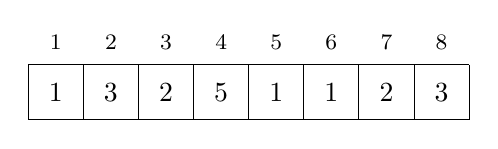
\begin{tikzpicture}[scale=0.7]
\draw (0,0) grid (8,1);

\node at (0.5,0.5) {$1$};
\node at (1.5,0.5) {$3$};
\node at (2.5,0.5) {$2$};
\node at (3.5,0.5) {$5$};
\node at (4.5,0.5) {$1$};
\node at (5.5,0.5) {$1$};
\node at (6.5,0.5) {$2$};
\node at (7.5,0.5) {$3$};

\footnotesize
\node at (0.5,1.4) {$1$};
\node at (1.5,1.4) {$2$};
\node at (2.5,1.4) {$3$};
\node at (3.5,1.4) {$4$};
\node at (4.5,1.4) {$5$};
\node at (5.5,1.4) {$6$};
\node at (6.5,1.4) {$7$};
\node at (7.5,1.4) {$8$};
\end{tikzpicture}
\end{center}
on alitaulukko, jossa lukujen summa on 8:
\begin{center}
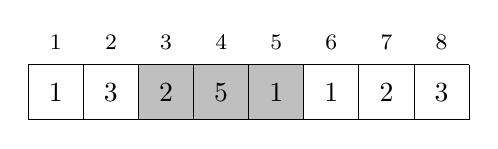
\begin{tikzpicture}[scale=0.7]
\fill[color=lightgray] (2,0) rectangle (5,1);
\draw (0,0) grid (8,1);

\node at (0.5,0.5) {$1$};
\node at (1.5,0.5) {$3$};
\node at (2.5,0.5) {$2$};
\node at (3.5,0.5) {$5$};
\node at (4.5,0.5) {$1$};
\node at (5.5,0.5) {$1$};
\node at (6.5,0.5) {$2$};
\node at (7.5,0.5) {$3$};

\footnotesize
\node at (0.5,1.4) {$1$};
\node at (1.5,1.4) {$2$};
\node at (2.5,1.4) {$3$};
\node at (3.5,1.4) {$4$};
\node at (4.5,1.4) {$5$};
\node at (5.5,1.4) {$6$};
\node at (6.5,1.4) {$7$};
\node at (7.5,1.4) {$8$};
\end{tikzpicture}
\end{center}

Osoittautuu, että tämän tehtävän voi ratkaista
ajassa $O(n)$ kahden osoittimen tekniikalla.
Ideana on käydä taulukkoa läpi kahden osoittimen
avulla, jotka rajaavat välin taulukosta.
Joka vuorolla vasen osoitin liikkuu
yhden askeleen eteenpäin ja oikea osoitin
liikkuu niin kauan eteenpäin kuin summa on enintään $x$.
Jos välin summaksi tulee tarkalleen $x$, ratkaisu on löytynyt.

Tarkastellaan esimerkkinä algoritmin toimintaa
seuraavassa taulukossa, kun tavoitteena on muodostaa summa $x=8$:
\begin{center}
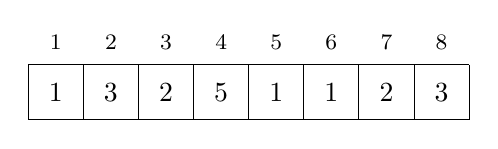
\begin{tikzpicture}[scale=0.7]
\draw (0,0) grid (8,1);

\node at (0.5,0.5) {$1$};
\node at (1.5,0.5) {$3$};
\node at (2.5,0.5) {$2$};
\node at (3.5,0.5) {$5$};
\node at (4.5,0.5) {$1$};
\node at (5.5,0.5) {$1$};
\node at (6.5,0.5) {$2$};
\node at (7.5,0.5) {$3$};

\footnotesize
\node at (0.5,1.4) {$1$};
\node at (1.5,1.4) {$2$};
\node at (2.5,1.4) {$3$};
\node at (3.5,1.4) {$4$};
\node at (4.5,1.4) {$5$};
\node at (5.5,1.4) {$6$};
\node at (6.5,1.4) {$7$};
\node at (7.5,1.4) {$8$};
\end{tikzpicture}
\end{center}

Aluksi osoittimet rajaavat taulukosta välin,
jonka summa on $1+3+2=6$.
Väli ei voi olla tätä suurempi,
koska seuraava luku 5 veisi summan yli $x$:n.

\begin{center}
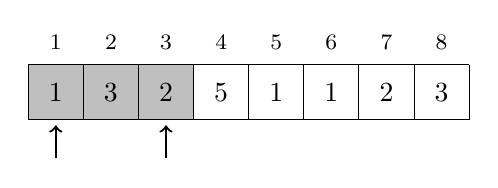
\begin{tikzpicture}[scale=0.7]
\fill[color=lightgray] (0,0) rectangle (3,1);
\draw (0,0) grid (8,1);

\node at (0.5,0.5) {$1$};
\node at (1.5,0.5) {$3$};
\node at (2.5,0.5) {$2$};
\node at (3.5,0.5) {$5$};
\node at (4.5,0.5) {$1$};
\node at (5.5,0.5) {$1$};
\node at (6.5,0.5) {$2$};
\node at (7.5,0.5) {$3$};

\draw[thick,->] (0.5,-0.7) -- (0.5,-0.1);
\draw[thick,->] (2.5,-0.7) -- (2.5,-0.1);

\footnotesize
\node at (0.5,1.4) {$1$};
\node at (1.5,1.4) {$2$};
\node at (2.5,1.4) {$3$};
\node at (3.5,1.4) {$4$};
\node at (4.5,1.4) {$5$};
\node at (5.5,1.4) {$6$};
\node at (6.5,1.4) {$7$};
\node at (7.5,1.4) {$8$};
\end{tikzpicture}
\end{center}

Seuraavaksi vasen osoitin siirtyy askeleen eteenpäin.
Oikea osoitin säilyy paikallaan, koska muuten
summa kasvaisi liian suureksi.

\begin{center}
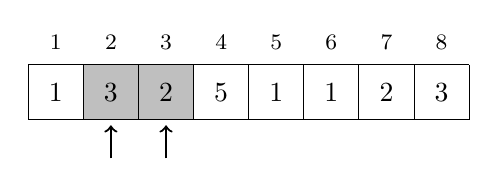
\begin{tikzpicture}[scale=0.7]
\fill[color=lightgray] (1,0) rectangle (3,1);
\draw (0,0) grid (8,1);

\node at (0.5,0.5) {$1$};
\node at (1.5,0.5) {$3$};
\node at (2.5,0.5) {$2$};
\node at (3.5,0.5) {$5$};
\node at (4.5,0.5) {$1$};
\node at (5.5,0.5) {$1$};
\node at (6.5,0.5) {$2$};
\node at (7.5,0.5) {$3$};

\draw[thick,->] (1.5,-0.7) -- (1.5,-0.1);
\draw[thick,->] (2.5,-0.7) -- (2.5,-0.1);

\footnotesize
\node at (0.5,1.4) {$1$};
\node at (1.5,1.4) {$2$};
\node at (2.5,1.4) {$3$};
\node at (3.5,1.4) {$4$};
\node at (4.5,1.4) {$5$};
\node at (5.5,1.4) {$6$};
\node at (6.5,1.4) {$7$};
\node at (7.5,1.4) {$8$};
\end{tikzpicture}
\end{center}

Vasen osoitin siirtyy taas askeleen eteenpäin
ja tällä kertaa oikea osoitin siirtyy kolme askelta
eteenpäin. Muodostuu summa $2+5+1=8$ eli taulukosta
on löytynyt väli, jonka lukujen summa on $x$.

\begin{center}
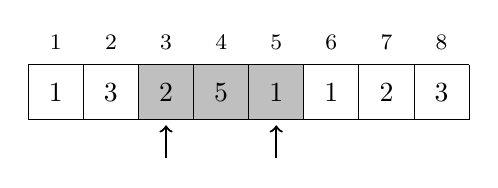
\begin{tikzpicture}[scale=0.7]
\fill[color=lightgray] (2,0) rectangle (5,1);
\draw (0,0) grid (8,1);

\node at (0.5,0.5) {$1$};
\node at (1.5,0.5) {$3$};
\node at (2.5,0.5) {$2$};
\node at (3.5,0.5) {$5$};
\node at (4.5,0.5) {$1$};
\node at (5.5,0.5) {$1$};
\node at (6.5,0.5) {$2$};
\node at (7.5,0.5) {$3$};

\draw[thick,->] (2.5,-0.7) -- (2.5,-0.1);
\draw[thick,->] (4.5,-0.7) -- (4.5,-0.1);

\footnotesize
\node at (0.5,1.4) {$1$};
\node at (1.5,1.4) {$2$};
\node at (2.5,1.4) {$3$};
\node at (3.5,1.4) {$4$};
\node at (4.5,1.4) {$5$};
\node at (5.5,1.4) {$6$};
\node at (6.5,1.4) {$7$};
\node at (7.5,1.4) {$8$};
\end{tikzpicture}
\end{center}

% Algoritmin toteutus näyttää seuraavalta:
% 
% \begin{lstlisting}
% int s = 0, b = 0;
% for (int a = 1; a <= n; a++) {
%     while (b<n && s+t[b+1] <= x) {
%         b++;
%         s += t[b];
%     }
%     if (s == x) {
%         // ratkaisu löytyi
%     }
%     s -= t[a];
% }
% \end{lstlisting}
% 
% Muuttujat $a$ ja $b$ sisältävät vasemman ja oikean
% osoittimen kohdan.
% Muuttuja $s$ taas laskee lukujen summan välillä.
% Joka askeleella $a$ liikkuu askeleen eteenpäin
% ja $b$ liikkuu niin kauan kuin summa on enintään $x$.

Algoritmin aikavaativuus riippuu siitä,
kauanko oikean osoittimen liikkuminen vie aikaa.
Tämä vaihtelee, koska oikea osoitin voi liikkua
minkä tahansa matkan eteenpäin taulukossa.
Kuitenkin oikea osoitin liikkuu \textit{yhteensä}
$O(n)$ askelta algoritmin aikana, koska se voi
liikkua vain eteenpäin.

Koska sekä vasen että oikea osoitin liikkuvat
$O(n)$ askelta algoritmin aikana,
algoritmin aikavaativuus on $O(n)$.

\subsubsection{Kahden luvun summa}

\index{2SUM-ongelma}

Annettuna on taulukko, jossa on $n$ kokonaislukua,
sekä kokonaisluku $x$.
Tehtävänä on etsiä taulukosta kaksi lukua,
joiden summa on $x$, tai todeta,
että tämä ei ole mahdollista.
Tämä ongelma tunnetaan tunnetaan nimellä
\key{2SUM} ja se ratkeaa tehokkaasti
kahden osoittimen tekniikalla.

Taulukon luvut järjestetään ensin
pienimmästä suurimpaan, minkä jälkeen
taulukkoa aletaan käydä läpi kahdella osoittimella,
jotka lähtevät liikkelle taulukon molemmista päistä.
Vasen osoitin aloittaa taulukon alusta ja
liikkuu joka vaiheessa askeleen eteenpäin.
Oikea osoitin taas aloittaa taulukon lopusta
ja peruuttaa vuorollaan taaksepäin, kunnes osoitinten
määrittämän välin lukujen summa on enintään $x$.
Jos summa on tarkalleen $x$, ratkaisu on löytynyt.

Tarkastellaan algoritmin toimintaa
seuraavassa taulukossa, kun tavoitteena on muodostaa
summa $x=12$:
\begin{center}
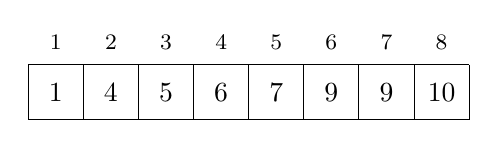
\begin{tikzpicture}[scale=0.7]
\draw (0,0) grid (8,1);

\node at (0.5,0.5) {$1$};
\node at (1.5,0.5) {$4$};
\node at (2.5,0.5) {$5$};
\node at (3.5,0.5) {$6$};
\node at (4.5,0.5) {$7$};
\node at (5.5,0.5) {$9$};
\node at (6.5,0.5) {$9$};
\node at (7.5,0.5) {$10$};

\footnotesize
\node at (0.5,1.4) {$1$};
\node at (1.5,1.4) {$2$};
\node at (2.5,1.4) {$3$};
\node at (3.5,1.4) {$4$};
\node at (4.5,1.4) {$5$};
\node at (5.5,1.4) {$6$};
\node at (6.5,1.4) {$7$};
\node at (7.5,1.4) {$8$};
\end{tikzpicture}
\end{center}

Seuraavassa on algoritmin aloitustilanne.
Lukujen summa on $1+10=11$, joka on pienempi
kuin $x$:n arvo.

\begin{center}
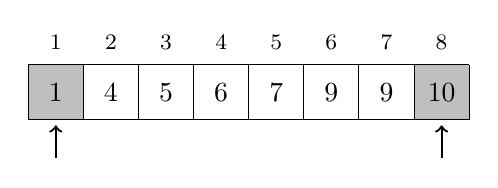
\begin{tikzpicture}[scale=0.7]
\fill[color=lightgray] (0,0) rectangle (1,1);
\fill[color=lightgray] (7,0) rectangle (8,1);
\draw (0,0) grid (8,1);

\node at (0.5,0.5) {$1$};
\node at (1.5,0.5) {$4$};
\node at (2.5,0.5) {$5$};
\node at (3.5,0.5) {$6$};
\node at (4.5,0.5) {$7$};
\node at (5.5,0.5) {$9$};
\node at (6.5,0.5) {$9$};
\node at (7.5,0.5) {$10$};

\draw[thick,->] (0.5,-0.7) -- (0.5,-0.1);
\draw[thick,->] (7.5,-0.7) -- (7.5,-0.1);

\footnotesize
\node at (0.5,1.4) {$1$};
\node at (1.5,1.4) {$2$};
\node at (2.5,1.4) {$3$};
\node at (3.5,1.4) {$4$};
\node at (4.5,1.4) {$5$};
\node at (5.5,1.4) {$6$};
\node at (6.5,1.4) {$7$};
\node at (7.5,1.4) {$8$};
\end{tikzpicture}
\end{center}

Seuraavaksi vasen osoitin liikkuu askeleen eteenpäin.
Oikea osoitin peruuttaa kolme askelta, minkä jälkeen
summana on $4+7=11$.

\begin{center}
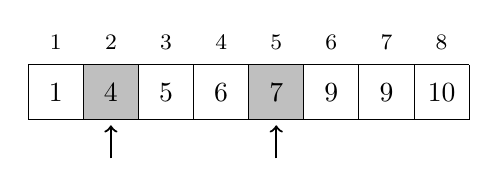
\begin{tikzpicture}[scale=0.7]
\fill[color=lightgray] (1,0) rectangle (2,1);
\fill[color=lightgray] (4,0) rectangle (5,1);
\draw (0,0) grid (8,1);

\node at (0.5,0.5) {$1$};
\node at (1.5,0.5) {$4$};
\node at (2.5,0.5) {$5$};
\node at (3.5,0.5) {$6$};
\node at (4.5,0.5) {$7$};
\node at (5.5,0.5) {$9$};
\node at (6.5,0.5) {$9$};
\node at (7.5,0.5) {$10$};

\draw[thick,->] (1.5,-0.7) -- (1.5,-0.1);
\draw[thick,->] (4.5,-0.7) -- (4.5,-0.1);

\footnotesize
\node at (0.5,1.4) {$1$};
\node at (1.5,1.4) {$2$};
\node at (2.5,1.4) {$3$};
\node at (3.5,1.4) {$4$};
\node at (4.5,1.4) {$5$};
\node at (5.5,1.4) {$6$};
\node at (6.5,1.4) {$7$};
\node at (7.5,1.4) {$8$};
\end{tikzpicture}
\end{center}

Sitten vasen osoitin siirtyy jälleen askeleen eteenpäin.
Oikea osoitin pysyy paikallaan ja ratkaisu $5+7=12$ on löytynyt.

\begin{center}
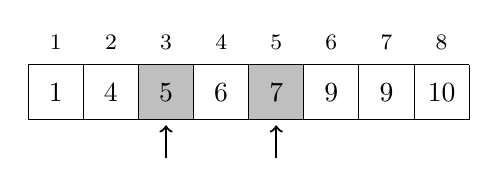
\begin{tikzpicture}[scale=0.7]
\fill[color=lightgray] (2,0) rectangle (3,1);
\fill[color=lightgray] (4,0) rectangle (5,1);
\draw (0,0) grid (8,1);

\node at (0.5,0.5) {$1$};
\node at (1.5,0.5) {$4$};
\node at (2.5,0.5) {$5$};
\node at (3.5,0.5) {$6$};
\node at (4.5,0.5) {$7$};
\node at (5.5,0.5) {$9$};
\node at (6.5,0.5) {$9$};
\node at (7.5,0.5) {$10$};

\draw[thick,->] (2.5,-0.7) -- (2.5,-0.1);
\draw[thick,->] (4.5,-0.7) -- (4.5,-0.1);

\footnotesize
\node at (0.5,1.4) {$1$};
\node at (1.5,1.4) {$2$};
\node at (2.5,1.4) {$3$};
\node at (3.5,1.4) {$4$};
\node at (4.5,1.4) {$5$};
\node at (5.5,1.4) {$6$};
\node at (6.5,1.4) {$7$};
\node at (7.5,1.4) {$8$};
\end{tikzpicture}
\end{center}

Algoritmin alussa taulukon järjestäminen vie
aikaa $O(n \log n)$.
Tämän jälkeen vasen osoitin liikkuu $O(n)$ askelta
eteenpäin ja oikea osoitin liikkuu $O(n)$ askelta
taaksepäin, mihin kuluu aikaa $O(n)$.
Algoritmin kokonaisaikavaativuus on siis $O(n \log n)$.

Huomaa, että tehtävän voi ratkaista myös 
toisella tavalla ajassa
$O(n \log n)$ binäärihaun avulla.
Tässä ratkaisussa jokaiselle taulukon luvulle
etsitään binäärihaulla toista lukua niin,
että lukujen summa olisi yhteensä $x$.
Binäärihaku suoritetaan $n$ kertaa ja
jokainen binäärihaku vie aikaa $O(\log n)$.

\index{3SUM-ongelma}
Hieman vaikeampi ongelma on \key{3SUM},
jossa taulukosta tuleekin etsiä kolme lukua,
joiden summa on $x$.
Tämä ongelma on mahdollista ratkaista ajassa $O(n^2)$.
Keksitkö, miten se tapahtuu?

\section{Lähin pienempi edeltäjä}

\index{lzhin pienempi edeltxjx@lähin pienempi edeltäjä}

Tasoitetun analyysin avulla arvioidaan usein
tietorakenteeseen kohdistuvien operaatioiden määrää.
Algoritmin operaatiot voivat jakautua epätasaisesti
niin, että useimmat operaatiot tehdään tietyssä
algoritmin vaiheessa, mutta operaatioiden
yhteismäärä on kuitenkin rajoitettu.

Tarkastellaan esimerkkinä ongelmaa,
jossa tehtävänä on etsiä kullekin taulukon
alkiolle
\key{lähin pienempi edeltäjä} eli
lähinnä oleva pienempi alkio taulukon alkuosassa.
On mahdollista, ettei tällaista alkiota ole olemassa,
jolloin algoritmin tulee huomata asia.
Osoittautuu, että tehtävä on mahdollista ratkaista
tehokkaasti ajassa $O(n)$ sopivan tietorakenteen avulla.

Tehokas ratkaisu tehtävään on käydä
taulukko läpi alusta loppuun ja pitää samalla yllä ketjua,
jonka ensimmäinen luku on käsiteltävä taulukon luku
ja jokainen seuraava luku on luvun lähin
pienempi edeltäjä.
Jos ketjussa on vain yksi luku,
käsiteltävällä luvulla ei ole pienempää edeltäjää.
Joka askeleella ketjun alusta poistetaan lukuja
niin kauan, kunnes ketjun ensimmäinen luku on 
pienempi kuin käsiteltävä taulukon luku tai ketju on tyhjä.
Tämän jälkeen käsiteltävä luku lisätään ketjun alkuun.

Tarkastellaan esimerkkinä algoritmin toimintaa
seuraavassa taulukossa:
\begin{center}
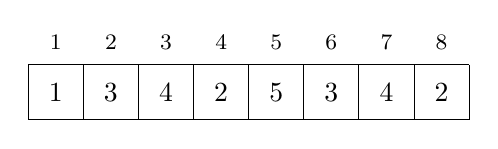
\begin{tikzpicture}[scale=0.7]
\draw (0,0) grid (8,1);

\node at (0.5,0.5) {$1$};
\node at (1.5,0.5) {$3$};
\node at (2.5,0.5) {$4$};
\node at (3.5,0.5) {$2$};
\node at (4.5,0.5) {$5$};
\node at (5.5,0.5) {$3$};
\node at (6.5,0.5) {$4$};
\node at (7.5,0.5) {$2$};

\footnotesize
\node at (0.5,1.4) {$1$};
\node at (1.5,1.4) {$2$};
\node at (2.5,1.4) {$3$};
\node at (3.5,1.4) {$4$};
\node at (4.5,1.4) {$5$};
\node at (5.5,1.4) {$6$};
\node at (6.5,1.4) {$7$};
\node at (7.5,1.4) {$8$};
\end{tikzpicture}
\end{center}

Aluksi luvut 1, 3 ja 4 liittyvät ketjuun, koska jokainen luku on
edellistä suurempi. Siis luvun 4 lähin pienempi edeltäjä on luku 3,
jonka lähin pienempi edeltäjä on puolestaan luku 1. Tilanne näyttää tältä:
\begin{center}
\begin{tikzpicture}[scale=0.7]
\fill[color=lightgray] (2,0) rectangle (3,1);
\draw (0,0) grid (8,1);

\node at (0.5,0.5) {$1$};
\node at (1.5,0.5) {$3$};
\node at (2.5,0.5) {$4$};
\node at (3.5,0.5) {$2$};
\node at (4.5,0.5) {$5$};
\node at (5.5,0.5) {$3$};
\node at (6.5,0.5) {$4$};
\node at (7.5,0.5) {$2$};

\draw[thick,->] (2.5,-0.25) .. controls (2.25,-1.00) and (1.75,-1.00) .. (1.6,-0.25);
\draw[thick,->] (1.4,-0.25) .. controls (1.25,-1.00) and (0.75,-1.00) .. (0.5,-0.25);

\footnotesize
\node at (0.5,1.4) {$1$};
\node at (1.5,1.4) {$2$};
\node at (2.5,1.4) {$3$};
\node at (3.5,1.4) {$4$};
\node at (4.5,1.4) {$5$};
\node at (5.5,1.4) {$6$};
\node at (6.5,1.4) {$7$};
\node at (7.5,1.4) {$8$};
\end{tikzpicture}
\end{center}

Taulukon seuraava luku 2 on pienempi kuin ketjun kaksi ensimmäistä lukua 4 ja 3.
Niinpä luvut 4 ja 3 poistetaan ketjusta, minkä jälkeen luku 2
lisätään ketjun alkuun. Sen lähin pienempi edeltäjä on luku 1:
\begin{center}
\begin{tikzpicture}[scale=0.7]
\fill[color=lightgray] (3,0) rectangle (4,1);
\draw (0,0) grid (8,1);

\node at (0.5,0.5) {$1$};
\node at (1.5,0.5) {$3$};
\node at (2.5,0.5) {$4$};
\node at (3.5,0.5) {$2$};
\node at (4.5,0.5) {$5$};
\node at (5.5,0.5) {$3$};
\node at (6.5,0.5) {$4$};
\node at (7.5,0.5) {$2$};

\draw[thick,->] (3.5,-0.25) .. controls (3.00,-1.00) and (1.00,-1.00) .. (0.5,-0.25);

\footnotesize
\node at (0.5,1.4) {$1$};
\node at (1.5,1.4) {$2$};
\node at (2.5,1.4) {$3$};
\node at (3.5,1.4) {$4$};
\node at (4.5,1.4) {$5$};
\node at (5.5,1.4) {$6$};
\node at (6.5,1.4) {$7$};
\node at (7.5,1.4) {$8$};
\end{tikzpicture}
\end{center}

Seuraava luku 5 on suurempi kuin luku 2,
joten se lisätään suoraan ketjun alkuun ja
sen lähin pienempi edeltäjä on luku 2:
\begin{center}
\begin{tikzpicture}[scale=0.7]
\fill[color=lightgray] (4,0) rectangle (5,1);
\draw (0,0) grid (8,1);

\node at (0.5,0.5) {$1$};
\node at (1.5,0.5) {$3$};
\node at (2.5,0.5) {$4$};
\node at (3.5,0.5) {$2$};
\node at (4.5,0.5) {$5$};
\node at (5.5,0.5) {$3$};
\node at (6.5,0.5) {$4$};
\node at (7.5,0.5) {$2$};

\draw[thick,->] (3.4,-0.25) .. controls (3.00,-1.00) and (1.00,-1.00) .. (0.5,-0.25);
\draw[thick,->] (4.5,-0.25) .. controls (4.25,-1.00) and (3.75,-1.00) .. (3.6,-0.25);

\footnotesize
\node at (0.5,1.4) {$1$};
\node at (1.5,1.4) {$2$};
\node at (2.5,1.4) {$3$};
\node at (3.5,1.4) {$4$};
\node at (4.5,1.4) {$5$};
\node at (5.5,1.4) {$6$};
\node at (6.5,1.4) {$7$};
\node at (7.5,1.4) {$8$};
\end{tikzpicture}
\end{center}

Algoritmi jatkaa samalla tavalla taulukon loppuun
ja selvittää jokaisen luvun lähimmän
pienemmän edeltäjän.
Mutta kuinka tehokas algoritmi on?

Algoritmin tehokkuus riippuu siitä,
kauanko ketjun käsittelyyn kuluu aikaa yhteensä.
Jos uusi luku on suurempi kuin ketjun ensimmäinen
luku, se vain lisätään ketjun alkuun,
mikä on tehokasta.
Joskus taas ketjussa voi olla useita
suurempia lukuja, joiden poistaminen vie aikaa.
Oleellista on kuitenkin, että jokainen
taulukossa oleva luku liittyy
tarkalleen kerran ketjuun ja poistuu
korkeintaan kerran ketjusta.
Niinpä jokainen luku aiheuttaa $O(1)$
ketjuun liittyvää operaatiota
ja algoritmin kokonaisaikavaativuus on $O(n)$.

\section{Liukuvan ikkunan minimi}

\index{liukuva ikkuna}
\index{liukuvan ikkunan minimi@liukuvan ikkunan minimi}

\key{Liukuva ikkuna} on taulukon halki kulkeva
aktiivinen alitaulukko, jonka pituus on vakio.
Jokaisessa liukuvan ikkunan sijainnissa
halutaan tyypillisesti laskea jotain tietoa
ikkunan alueelle osuvista alkioista.
Kiinnostava tehtävä on pitää yllä
\key{liukuvan ikkunan minimiä}.
Tämä tarkoittaa, että jokaisessa liukuvan ikkunan
sijainnissa tulee ilmoittaa pienin alkio
ikkunan alueella.

Liukuvan ikkunan minimit voi laskea
lähes samalla tavalla kuin lähimmät
pienimmät edeltäjät.
Ideana on pitää yllä ketjua, jonka alussa
on ikkunan viimeinen luku ja jossa jokainen
luku on edellistä pienempi. Joka vaiheessa
ketjun viimeinen luku on ikkunan pienin luku.
Kun liukuva ikkuna liikkuu eteenpäin ja välille
tulee uusi luku, ketjusta poistetaan kaikki luvut,
jotka ovat uutta lukua suurempia.
Tämän jälkeen uusi luku lisätään ketjun alkuun.
Lisäksi jos ketjun viimeinen luku ei enää kuulu
välille, se poistetaan ketjusta.

Tarkastellaan esimerkkinä, kuinka algoritmi selvittää
minimit seuraavassa taulukossa,
kun ikkunan koko $k=4$.

\begin{center}
\begin{tikzpicture}[scale=0.7]
\draw (0,0) grid (8,1);

\node at (0.5,0.5) {$2$};
\node at (1.5,0.5) {$1$};
\node at (2.5,0.5) {$4$};
\node at (3.5,0.5) {$5$};
\node at (4.5,0.5) {$3$};
\node at (5.5,0.5) {$4$};
\node at (6.5,0.5) {$1$};
\node at (7.5,0.5) {$2$};

\footnotesize
\node at (0.5,1.4) {$1$};
\node at (1.5,1.4) {$2$};
\node at (2.5,1.4) {$3$};
\node at (3.5,1.4) {$4$};
\node at (4.5,1.4) {$5$};
\node at (5.5,1.4) {$6$};
\node at (6.5,1.4) {$7$};
\node at (7.5,1.4) {$8$};
\end{tikzpicture}
\end{center}

Liukuva ikkuna aloittaa matkansa taulukon vasemmasta reunasta.
Ensimmäisessä ikkunan sijainnissa pienin luku on 1:
\begin{center}
\begin{tikzpicture}[scale=0.7]
\fill[color=lightgray] (0,0) rectangle (4,1);
\draw (0,0) grid (8,1);

\node at (0.5,0.5) {$2$};
\node at (1.5,0.5) {$1$};
\node at (2.5,0.5) {$4$};
\node at (3.5,0.5) {$5$};
\node at (4.5,0.5) {$3$};
\node at (5.5,0.5) {$4$};
\node at (6.5,0.5) {$1$};
\node at (7.5,0.5) {$2$};

\footnotesize
\node at (0.5,1.4) {$1$};
\node at (1.5,1.4) {$2$};
\node at (2.5,1.4) {$3$};
\node at (3.5,1.4) {$4$};
\node at (4.5,1.4) {$5$};
\node at (5.5,1.4) {$6$};
\node at (6.5,1.4) {$7$};
\node at (7.5,1.4) {$8$};

\draw[thick,->] (3.5,-0.25) .. controls (3.25,-1.00) and (2.75,-1.00) .. (2.6,-0.25);
\draw[thick,->] (2.4,-0.25) .. controls (2.25,-1.00) and (1.75,-1.00) .. (1.5,-0.25);

\end{tikzpicture}
\end{center}

Kun ikkuna siirtyy eteenpäin, mukaan tulee luku 3,
joka on pienempi kuin luvut 5 ja 4 ketjun alussa.
Niinpä luvut 5 ja 4 poistuvat ketjusta ja luku 3
siirtyy sen alkuun. Pienin luku on edelleen 1.
\begin{center}
\begin{tikzpicture}[scale=0.7]
\fill[color=lightgray] (1,0) rectangle (5,1);
\draw (0,0) grid (8,1);

\node at (0.5,0.5) {$2$};
\node at (1.5,0.5) {$1$};
\node at (2.5,0.5) {$4$};
\node at (3.5,0.5) {$5$};
\node at (4.5,0.5) {$3$};
\node at (5.5,0.5) {$4$};
\node at (6.5,0.5) {$1$};
\node at (7.5,0.5) {$2$};

\footnotesize
\node at (0.5,1.4) {$1$};
\node at (1.5,1.4) {$2$};
\node at (2.5,1.4) {$3$};
\node at (3.5,1.4) {$4$};
\node at (4.5,1.4) {$5$};
\node at (5.5,1.4) {$6$};
\node at (6.5,1.4) {$7$};
\node at (7.5,1.4) {$8$};

\draw[thick,->] (4.5,-0.25) .. controls (4.25,-1.00) and (1.75,-1.00) .. (1.5,-0.25);

\end{tikzpicture}
\end{center}

Ikkuna siirtyy taas eteenpäin, minkä seurauksena pienin luku 1
putoaa pois ikkunasta. Niinpä se poistetaan ketjun lopusta
ja uusi pienin luku on 3. Lisäksi uusi ikkunaan tuleva luku 4
lisätään ketjun alkuun.
\begin{center}
\begin{tikzpicture}[scale=0.7]
\fill[color=lightgray] (2,0) rectangle (6,1);
\draw (0,0) grid (8,1);

\node at (0.5,0.5) {$2$};
\node at (1.5,0.5) {$1$};
\node at (2.5,0.5) {$4$};
\node at (3.5,0.5) {$5$};
\node at (4.5,0.5) {$3$};
\node at (5.5,0.5) {$4$};
\node at (6.5,0.5) {$1$};
\node at (7.5,0.5) {$2$};

\footnotesize
\node at (0.5,1.4) {$1$};
\node at (1.5,1.4) {$2$};
\node at (2.5,1.4) {$3$};
\node at (3.5,1.4) {$4$};
\node at (4.5,1.4) {$5$};
\node at (5.5,1.4) {$6$};
\node at (6.5,1.4) {$7$};
\node at (7.5,1.4) {$8$};

\draw[thick,->] (5.5,-0.25) .. controls (5.25,-1.00) and (4.75,-1.00) .. (4.5,-0.25);
\end{tikzpicture}
\end{center}

Seuraavaksi ikkunaan tuleva luku 1 on pienempi
kuin kaikki ketjussa olevat luvut.
Tämän seurauksena koko ketju tyhjentyy ja
siihen jää vain luku 1:
\begin{center}
\begin{tikzpicture}[scale=0.7]
\fill[color=lightgray] (3,0) rectangle (7,1);
\draw (0,0) grid (8,1);

\node at (0.5,0.5) {$2$};
\node at (1.5,0.5) {$1$};
\node at (2.5,0.5) {$4$};
\node at (3.5,0.5) {$5$};
\node at (4.5,0.5) {$3$};
\node at (5.5,0.5) {$4$};
\node at (6.5,0.5) {$1$};
\node at (7.5,0.5) {$2$};

\footnotesize
\node at (0.5,1.4) {$1$};
\node at (1.5,1.4) {$2$};
\node at (2.5,1.4) {$3$};
\node at (3.5,1.4) {$4$};
\node at (4.5,1.4) {$5$};
\node at (5.5,1.4) {$6$};
\node at (6.5,1.4) {$7$};
\node at (7.5,1.4) {$8$};

\fill[color=black] (6.5,-0.25) circle (0.1);

%\draw[thick,->] (5.5,-0.25) .. controls (5.25,-1.00) and (4.75,-1.00) .. (4.5,-0.25);
\end{tikzpicture}
\end{center}

Lopuksi ikkuna saapuu viimeiseen sijaintiinsa.
Luku 2 lisätään ketjun alkuun,
mutta ikkunan pienin luku on edelleen 1.
\begin{center}
\begin{tikzpicture}[scale=0.7]
\fill[color=lightgray] (4,0) rectangle (8,1);
\draw (0,0) grid (8,1);

\node at (0.5,0.5) {$2$};
\node at (1.5,0.5) {$1$};
\node at (2.5,0.5) {$4$};
\node at (3.5,0.5) {$5$};
\node at (4.5,0.5) {$3$};
\node at (5.5,0.5) {$4$};
\node at (6.5,0.5) {$1$};
\node at (7.5,0.5) {$2$};

\footnotesize
\node at (0.5,1.4) {$1$};
\node at (1.5,1.4) {$2$};
\node at (2.5,1.4) {$3$};
\node at (3.5,1.4) {$4$};
\node at (4.5,1.4) {$5$};
\node at (5.5,1.4) {$6$};
\node at (6.5,1.4) {$7$};
\node at (7.5,1.4) {$8$};

\draw[thick,->] (7.5,-0.25) .. controls (7.25,-1.00) and (6.75,-1.00) .. (6.5,-0.25);
\end{tikzpicture}
\end{center}

Tässäkin algoritmissa jokainen taulukon luku lisätään
ketjuun tarkalleen kerran ja poistetaan ketjusta korkeintaan kerran,
joko ketjun alusta tai ketjun lopusta.
Niinpä algoritmin kokonaisaikavaativuus on $O(n)$.




\chapter{Välikyselyt}

\index{välikysely}
\index{summakysely}
\index{minimikysely}
\index{maksimikysely}

\key{Välikysely} kohdistuu
taulukkoon, jonka sisältönä on lukuja.
Kyselyssä annetaan tietty taulukon väli $[a,b]$
ja tehtävänä on laskea haluttu tieto välillä olevista luvuista.
Tavallisia välikyselyitä ovat:

\begin{itemize}
\item \key{summakysely}: laske välin $[a,b]$ lukujen summa
\item \key{minimikysely}: etsi pienin luku välillä $[a,b]$
\item \key{maksimikysely}: etsi suurin luku välillä $[a,b]$
\end{itemize}

\noindent
Tarkastellaan esimerkkinä seuraavan taulukon väliä $[4,7]$:

\begin{center}
\begin{tikzpicture}[scale=0.7]
\fill[color=lightgray] (3,0) rectangle (7,1);
\draw (0,0) grid (8,1);

\node at (0.5,0.5) {$1$};
\node at (1.5,0.5) {$3$};
\node at (2.5,0.5) {$8$};
\node at (3.5,0.5) {$4$};
\node at (4.5,0.5) {$6$};
\node at (5.5,0.5) {$1$};
\node at (6.5,0.5) {$3$};
\node at (7.5,0.5) {$4$};

\footnotesize
\node at (0.5,1.4) {$1$};
\node at (1.5,1.4) {$2$};
\node at (2.5,1.4) {$3$};
\node at (3.5,1.4) {$4$};
\node at (4.5,1.4) {$5$};
\node at (5.5,1.4) {$6$};
\node at (6.5,1.4) {$7$};
\node at (7.5,1.4) {$8$};
\end{tikzpicture}
\end{center}

Välin $[4,7]$ summa on $4+6+1+3=14$, minimi on $1$
ja maksimi on $6$.

Helppo tapa vastata välikyselyyn on
käydä läpi kaikki välin luvut silmukalla.
Esimerkiksi seuraava funktio toteuttaa summakyselyn:

\begin{lstlisting}
int summa(int a, int b) {
    int s = 0;
    for (int i = a; i <= b; i++) {
        s += t[i];
    }
    return s;
}
\end{lstlisting}

Yllä oleva funktio toteuttaa summakyselyn
ajassa $O(n)$, mikä on hidasta,
jos taulukko on suuri ja kyselyitä tulee paljon.
Tässä luvussa opimme, miten välikyselyitä pystyy
toteuttamaan huomattavasti nopeammin.

\section{Staattiset kyselyt}

Aloitamme yksinkertaisesta
tilanteesta, jossa taulukko on staattinen
eli sen sisältö ei muutu kyselyiden välillä.
Tällöin riittää muodostaa ennen kyselyitä
taulukon pohjalta tietorakenne,
josta voi selvittää tehokkaasti vastauksen mihin tahansa väliin
kohdistuvaan kyselyyn.

\subsubsection{Summakysely}

\index{summataulukko}

Summakyselyyn on mahdollista vastata tehokkaasti
muodostamalla taulukosta etukäteen \key{summataulukko},
jonka kohdassa $k$ on taulukon välin $[1,k]$ summa.
Tämän jälkeen minkä tahansa välin $[a,b]$
summan saa laskettua $O(1)$-ajassa
summataulukkoa käyttäen.

Esimerkiksi taulukon
\begin{center}
\begin{tikzpicture}[scale=0.7]
%\fill[color=lightgray] (3,0) rectangle (7,1);
\draw (0,0) grid (8,1);

\node at (0.5,0.5) {$1$};
\node at (1.5,0.5) {$3$};
\node at (2.5,0.5) {$4$};
\node at (3.5,0.5) {$8$};
\node at (4.5,0.5) {$6$};
\node at (5.5,0.5) {$1$};
\node at (6.5,0.5) {$4$};
\node at (7.5,0.5) {$2$};

\footnotesize
\node at (0.5,1.4) {$1$};
\node at (1.5,1.4) {$2$};
\node at (2.5,1.4) {$3$};
\node at (3.5,1.4) {$4$};
\node at (4.5,1.4) {$5$};
\node at (5.5,1.4) {$6$};
\node at (6.5,1.4) {$7$};
\node at (7.5,1.4) {$8$};
\end{tikzpicture}
\end{center}

summataulukko on seuraava:

\begin{center}
\begin{tikzpicture}[scale=0.7]
%\fill[color=lightgray] (3,0) rectangle (7,1);
\draw (0,0) grid (8,1);

\node at (0.5,0.5) {$1$};
\node at (1.5,0.5) {$4$};
\node at (2.5,0.5) {$8$};
\node at (3.5,0.5) {$16$};
\node at (4.5,0.5) {$22$};
\node at (5.5,0.5) {$23$};
\node at (6.5,0.5) {$27$};
\node at (7.5,0.5) {$29$};


\footnotesize
\node at (0.5,1.4) {$1$};
\node at (1.5,1.4) {$2$};
\node at (2.5,1.4) {$3$};
\node at (3.5,1.4) {$4$};
\node at (4.5,1.4) {$5$};
\node at (5.5,1.4) {$6$};
\node at (6.5,1.4) {$7$};
\node at (7.5,1.4) {$8$};
\end{tikzpicture}
\end{center}

Seuraava koodi muodostaa taulukosta \texttt{t}
summataulukon \texttt{s} ajassa $O(n)$:

\begin{lstlisting}
for (int i = 1; i <= n; i++) {
    s[i] = s[i-1]+t[i];
}
\end{lstlisting}

Tämän jälkeen summakyselyyn voi vastata
ajassa $O(1)$ seuraavasti:

\begin{lstlisting}
int summa(int a, int b) {
    return s[b]-s[a-1];
}
\end{lstlisting}

Ideana on laskea välin $[a,b]$ summa 
laskemalla ensin välin $[1,b]$ summa
ja poistamalla siitä sitten välin $[1,a-1]$ summa.
Summataulukosta riittää hakea kaksi arvoa
ja aikaa kuluu vain $O(1)$.
Huomaa, että 1-indeksoinnin ansiosta
yllä oleva toteutus toimii myös tapauksessa $a=1$,
kunhan $\texttt{s}[0]=0$.

Tarkastellaan esimerkiksi väliä $[4,7]$:
\begin{center}
\begin{tikzpicture}[scale=0.7]
\fill[color=lightgray] (3,0) rectangle (7,1);
\draw (0,0) grid (8,1);

\node at (0.5,0.5) {$1$};
\node at (1.5,0.5) {$3$};
\node at (2.5,0.5) {$4$};
\node at (3.5,0.5) {$8$};
\node at (4.5,0.5) {$6$};
\node at (5.5,0.5) {$1$};
\node at (6.5,0.5) {$4$};
\node at (7.5,0.5) {$2$};

\footnotesize
\node at (0.5,1.4) {$1$};
\node at (1.5,1.4) {$2$};
\node at (2.5,1.4) {$3$};
\node at (3.5,1.4) {$4$};
\node at (4.5,1.4) {$5$};
\node at (5.5,1.4) {$6$};
\node at (6.5,1.4) {$7$};
\node at (7.5,1.4) {$8$};
\end{tikzpicture}
\end{center}
Välin $[4,7]$ summa on $8+6+1+4=19$.
Tämän saa laskettua tehokkaasti summataulukosta
etsimällä välien $[1,3]$ ja $[1,7]$ summat:
\begin{center}
\begin{tikzpicture}[scale=0.7]
\fill[color=lightgray] (2,0) rectangle (3,1);
\fill[color=lightgray] (6,0) rectangle (7,1);
\draw (0,0) grid (8,1);

\node at (0.5,0.5) {$1$};
\node at (1.5,0.5) {$4$};
\node at (2.5,0.5) {$8$};
\node at (3.5,0.5) {$16$};
\node at (4.5,0.5) {$22$};
\node at (5.5,0.5) {$23$};
\node at (6.5,0.5) {$27$};
\node at (7.5,0.5) {$29$};


\footnotesize
\node at (0.5,1.4) {$1$};
\node at (1.5,1.4) {$2$};
\node at (2.5,1.4) {$3$};
\node at (3.5,1.4) {$4$};
\node at (4.5,1.4) {$5$};
\node at (5.5,1.4) {$6$};
\node at (6.5,1.4) {$7$};
\node at (7.5,1.4) {$8$};
\end{tikzpicture}
\end{center}
Välin $[4,7]$ summa on siis $27-8=19$.

\subsubsection{Kaksiulotteinen taulukko}

Summataulukon idean voi yleistää
myös kaksiulotteiseen taulukkoon,
jolloin summataulukosta voi laskea
minkä tahansa suorakulmaisen alueen
summan $O(1)$-ajassa.
Ideana on tallentaa summataulukkoon summia
alueista, jotka alkavat taulukon vasemmasta yläkulmasta.

Seuraava ruudukko havainnollistaa asiaa:
\\
\begin{center}
\begin{tikzpicture}[scale=0.55]
\draw[fill=lightgray] (3,2) rectangle (7,5);
\draw (0,0) grid (10,7);
%\draw[line width=2pt] (3,2) rectangle (7,5);
\node[anchor=center] at (6.5, 2.5) {$A$};
\node[anchor=center] at (2.5, 2.5) {$B$};
\node[anchor=center] at (6.5, 5.5) {$C$};
\node[anchor=center] at (2.5, 5.5) {$D$};
\end{tikzpicture}
\end{center}

Harmaan suorakulmion summan saa laskettua kaavalla

\[S(A) - S(B) - S(C) + S(D),\]

missä $S(X)$ tarkoittaa summaa vasemmasta
yläkulmasta kirjaimen $X$ osoittamaan kohtaan asti.

\subsubsection{Minimikysely}

Myös minimikyselyyn on mahdollista
vastata $O(1)$-ajassa sopivan esikäsittelyn avulla,
joskin tämä on vaikeampaa kuin summakyselyssä.
Huomaa, että minimikysely ja maksimikysely on
mahdollista toteuttaa aina samalla tavalla,
joten riittää keskittyä minimikyselyn toteutukseen. 

Ideana on laskea etukäteen taulukon jokaiselle
$2^k$-kokoiselle välille, mikä on kyseisen välin minimi.
Esimerkiksi taulukosta

\begin{center}
\begin{tikzpicture}[scale=0.7]
\draw (0,0) grid (8,1);

\node at (0.5,0.5) {$1$};
\node at (1.5,0.5) {$3$};
\node at (2.5,0.5) {$4$};
\node at (3.5,0.5) {$8$};
\node at (4.5,0.5) {$6$};
\node at (5.5,0.5) {$1$};
\node at (6.5,0.5) {$4$};
\node at (7.5,0.5) {$2$};

\footnotesize
\node at (0.5,1.4) {$1$};
\node at (1.5,1.4) {$2$};
\node at (2.5,1.4) {$3$};
\node at (3.5,1.4) {$4$};
\node at (4.5,1.4) {$5$};
\node at (5.5,1.4) {$6$};
\node at (6.5,1.4) {$7$};
\node at (7.5,1.4) {$8$};
\end{tikzpicture}
\end{center}
lasketaan seuraavat minimit:

\begin{center}
\begin{tabular}{ccc}

\begin{tabular}{ccc}
väli & koko & minimi \\
\hline
$[1,1]$ & 1 & 1 \\
$[2,2]$ & 1 & 3 \\
$[3,3]$ & 1 & 4 \\
$[4,4]$ & 1 & 8 \\
$[5,5]$ & 1 & 6 \\
$[6,6]$ & 1 & 1 \\
$[7,7]$ & 1 & 4 \\
$[8,8]$ & 1 & 2 \\
\end{tabular}

&

\begin{tabular}{ccc}
väli & koko & minimi \\
\hline
$[1,2]$ & 2 & 1 \\
$[2,3]$ & 2 & 3 \\
$[3,4]$ & 2 & 4 \\
$[4,5]$ & 2 & 6 \\
$[5,6]$ & 2 & 1 \\
$[6,7]$ & 2 & 1 \\
$[7,8]$ & 2 & 2 \\
\\
\end{tabular}

&

\begin{tabular}{ccc}
väli & koko & minimi \\
\hline
$[1,4]$ & 4 & 1 \\
$[2,5]$ & 4 & 3 \\
$[3,6]$ & 4 & 1 \\
$[4,7]$ & 4 & 1 \\
$[5,8]$ & 4 & 1 \\
$[1,8]$ & 8 & 1 \\
\\
\\
\end{tabular}

\end{tabular}

\end{center}

Taulukon $2^k$-välien määrä on $O(n \log n)$,
koska jokaisesta taulukon kohdasta alkaa
$O(\log n)$ väliä.
Kaikkien $2^k$-välien minimit pystytään laskemaan
ajassa $O(n \log n)$, koska jokainen $2^k$-väli
muodostuu kahdesta $2^{k-1}$ välistä ja
$2^k$-välin minimi on pienempi $2^{k-1}$-välien minimeistä.

Tämän jälkeen minkä tahansa välin $[a,b]$ minimin
saa laskettua $O(1)$-ajassa miniminä kahdesta $2^k$-välistä,
missä $k=\lfloor \log_2(b-a+1) \rfloor$.
Ensimmäinen väli alkaa kohdasta $a$
ja toinen väli päättyy kohtaan $b$.
Parametri $k$ on valittu niin,
että kaksi $2^k$-kokoista väliä
kattaa koko välin $[a,b]$.

Tarkastellaan esimerkiksi väliä $[2,7]$:
\begin{center}
\begin{tikzpicture}[scale=0.7]
\fill[color=lightgray] (1,0) rectangle (7,1);
\draw (0,0) grid (8,1);

\node at (0.5,0.5) {$1$};
\node at (1.5,0.5) {$3$};
\node at (2.5,0.5) {$4$};
\node at (3.5,0.5) {$8$};
\node at (4.5,0.5) {$6$};
\node at (5.5,0.5) {$1$};
\node at (6.5,0.5) {$4$};
\node at (7.5,0.5) {$2$};

\footnotesize
\node at (0.5,1.4) {$1$};
\node at (1.5,1.4) {$2$};
\node at (2.5,1.4) {$3$};
\node at (3.5,1.4) {$4$};
\node at (4.5,1.4) {$5$};
\node at (5.5,1.4) {$6$};
\node at (6.5,1.4) {$7$};
\node at (7.5,1.4) {$8$};
\end{tikzpicture}
\end{center}
Välin $[2,7]$ pituus on 6 ja $\lfloor \log_2(6) \rfloor = 2$.
Niinpä välin minimin saa selville kahden 4-pituisen
välin minimistä.
Välit ovat $[2,5]$ ja $[4,7]$:
\begin{center}
\begin{tikzpicture}[scale=0.7]
\fill[color=lightgray] (1,0) rectangle (5,1);
\draw (0,0) grid (8,1);

\node at (0.5,0.5) {$1$};
\node at (1.5,0.5) {$3$};
\node at (2.5,0.5) {$4$};
\node at (3.5,0.5) {$8$};
\node at (4.5,0.5) {$6$};
\node at (5.5,0.5) {$1$};
\node at (6.5,0.5) {$4$};
\node at (7.5,0.5) {$2$};

\footnotesize
\node at (0.5,1.4) {$1$};
\node at (1.5,1.4) {$2$};
\node at (2.5,1.4) {$3$};
\node at (3.5,1.4) {$4$};
\node at (4.5,1.4) {$5$};
\node at (5.5,1.4) {$6$};
\node at (6.5,1.4) {$7$};
\node at (7.5,1.4) {$8$};
\end{tikzpicture}
\end{center}
\begin{center}
\begin{tikzpicture}[scale=0.7]
\fill[color=lightgray] (3,0) rectangle (7,1);
\draw (0,0) grid (8,1);

\node at (0.5,0.5) {$1$};
\node at (1.5,0.5) {$3$};
\node at (2.5,0.5) {$4$};
\node at (3.5,0.5) {$8$};
\node at (4.5,0.5) {$6$};
\node at (5.5,0.5) {$1$};
\node at (6.5,0.5) {$4$};
\node at (7.5,0.5) {$2$};


\footnotesize
\node at (0.5,1.4) {$1$};
\node at (1.5,1.4) {$2$};
\node at (2.5,1.4) {$3$};
\node at (3.5,1.4) {$4$};
\node at (4.5,1.4) {$5$};
\node at (5.5,1.4) {$6$};
\node at (6.5,1.4) {$7$};
\node at (7.5,1.4) {$8$};
\end{tikzpicture}
\end{center}
Välin $[2,5]$ minimi on 3 ja välin $[4,7]$ minimi on 1.
Tämän seurauksena välin $[2,7]$ minimi on pienempi näistä eli 1.

Mainittakoon, että $O(1)$-aikaiset minimikyselyt pystyy
toteuttamaan myös niin, että esikäsittely vie aikaa
vain $O(n)$ eikä $O(n \log n)$.
Tämä on kuitenkin selvästi vaikeampaa, eikä 
sillä ole merkitystä kisakoodauksessa.

\section{Binääri-indeksipuu}

\index{binääri-indeksipuu}
\index{Fenwick-puu}

\key{Binääri-indeksipuu} eli \key{Fenwick-puu} on
summataulukkoa muistuttava tietorakenne,
joka toteuttaa kaksi operaatiota:
taulukon välin $[a,b]$ summakysely
sekä taulukon kohdassa $k$ olevan luvun päivitys.
Kummankin operaation aikavaativuus on $O(\log n)$.

Binääri-indeksipuun etuna summataulukkoon verrattuna on,
että taulukkoa pystyy päivittämään tehokkaasti
summakyselyiden välissä.
Summataulukossa tämä ei olisi mahdollista,
vaan koko summataulukko tulisi muodostaa uudestaan $O(n)$-ajassa
taulukon päivityksen jälkeen.

\subsubsection{Rakenne}

Binääri-indeksipuu on taulukko, jonka
kohdassa $k$ on kohtaan $k$ päättyvän välin lukujen summa
alkuperäisessä taulukossa.
Välin pituus on suurin 2:n potenssi, jolla $k$ on jaollinen.
Esimerkiksi jos $k=6$, välin pituus on 2, koska
6 on jaollinen 2:lla mutta ei ole jaollinen 4:llä.

\begin{samepage}
Esimerkiksi taulukkoa
\begin{center}
\begin{tikzpicture}[scale=0.7]
\draw (0,0) grid (8,1);

\node at (0.5,0.5) {$1$};
\node at (1.5,0.5) {$3$};
\node at (2.5,0.5) {$4$};
\node at (3.5,0.5) {$8$};
\node at (4.5,0.5) {$6$};
\node at (5.5,0.5) {$1$};
\node at (6.5,0.5) {$4$};
\node at (7.5,0.5) {$2$};

\footnotesize
\node at (0.5,1.4) {$1$};
\node at (1.5,1.4) {$2$};
\node at (2.5,1.4) {$3$};
\node at (3.5,1.4) {$4$};
\node at (4.5,1.4) {$5$};
\node at (5.5,1.4) {$6$};
\node at (6.5,1.4) {$7$};
\node at (7.5,1.4) {$8$};
\end{tikzpicture}
\end{center}
\end{samepage}

vastaava binääri-indeksipuu on seuraava:
\begin{center}
\begin{tikzpicture}[scale=0.7]
%\fill[color=lightgray] (3,0) rectangle (7,1);
\draw (0,0) grid (8,1);

\node at (0.5,0.5) {$1$};
\node at (1.5,0.5) {$4$};
\node at (2.5,0.5) {$4$};
\node at (3.5,0.5) {$16$};
\node at (4.5,0.5) {$6$};
\node at (5.5,0.5) {$7$};
\node at (6.5,0.5) {$4$};
\node at (7.5,0.5) {$29$};

\footnotesize
\node at (0.5,1.4) {$1$};
\node at (1.5,1.4) {$2$};
\node at (2.5,1.4) {$3$};
\node at (3.5,1.4) {$4$};
\node at (4.5,1.4) {$5$};
\node at (5.5,1.4) {$6$};
\node at (6.5,1.4) {$7$};
\node at (7.5,1.4) {$8$};

\draw[->,thick] (0.5,-0.9) -- (0.5,-0.1);
\draw[->,thick] (2.5,-0.9) -- (2.5,-0.1);
\draw[->,thick] (4.5,-0.9) -- (4.5,-0.1);
\draw[->,thick] (6.5,-0.9) -- (6.5,-0.1);
\draw[->,thick] (1.5,-1.9) -- (1.5,-0.1);
\draw[->,thick] (5.5,-1.9) -- (5.5,-0.1);
\draw[->,thick] (3.5,-2.9) -- (3.5,-0.1);
\draw[->,thick] (7.5,-3.9) -- (7.5,-0.1);

\draw (0,-1) -- (1,-1) -- (1,-1.5) -- (0,-1.5) -- (0,-1);
\draw (2,-1) -- (3,-1) -- (3,-1.5) -- (2,-1.5) -- (2,-1);
\draw (4,-1) -- (5,-1) -- (5,-1.5) -- (4,-1.5) -- (4,-1);
\draw (6,-1) -- (7,-1) -- (7,-1.5) -- (6,-1.5) -- (6,-1);
\draw (0,-2) -- (2,-2) -- (2,-2.5) -- (0,-2.5) -- (0,-2);
\draw (4,-2) -- (6,-2) -- (6,-2.5) -- (4,-2.5) -- (4,-2);
\draw (0,-3) -- (4,-3) -- (4,-3.5) -- (0,-3.5) -- (0,-3);
\draw (0,-4) -- (8,-4) -- (8,-4.5) -- (0,-4.5) -- (0,-4);
\end{tikzpicture}
\end{center}

Esimerkiksi binääri-indeksipuun kohdassa 6 on luku 7,
koska välin $[5,6]$ lukujen summa on $6+1=7$.

\subsubsection{Summakysely}

Binääri-indeksipuun perusoperaatio on välin $[1,k]$
summan laskeminen, missä $k$ on mikä tahansa taulukon kohta.
Tällaisen summan pystyy muodostamaan aina laskemalla yhteen
puussa olevia välien summia.

Esimerkiksi välin $[1,7]$
summa muodostuu seuraavista summista:
\begin{center}
\begin{tikzpicture}[scale=0.7]
%\fill[color=lightgray] (3,0) rectangle (7,1);
\draw (0,0) grid (8,1);

\node at (0.5,0.5) {$1$};
\node at (1.5,0.5) {$4$};
\node at (2.5,0.5) {$4$};
\node at (3.5,0.5) {$16$};
\node at (4.5,0.5) {$6$};
\node at (5.5,0.5) {$7$};
\node at (6.5,0.5) {$4$};
\node at (7.5,0.5) {$29$};

\footnotesize
\node at (0.5,1.4) {$1$};
\node at (1.5,1.4) {$2$};
\node at (2.5,1.4) {$3$};
\node at (3.5,1.4) {$4$};
\node at (4.5,1.4) {$5$};
\node at (5.5,1.4) {$6$};
\node at (6.5,1.4) {$7$};
\node at (7.5,1.4) {$8$};

\draw[->,thick] (0.5,-0.9) -- (0.5,-0.1);
\draw[->,thick] (2.5,-0.9) -- (2.5,-0.1);
\draw[->,thick] (4.5,-0.9) -- (4.5,-0.1);
\draw[->,thick] (6.5,-0.9) -- (6.5,-0.1);
\draw[->,thick] (1.5,-1.9) -- (1.5,-0.1);
\draw[->,thick] (5.5,-1.9) -- (5.5,-0.1);
\draw[->,thick] (3.5,-2.9) -- (3.5,-0.1);
\draw[->,thick] (7.5,-3.9) -- (7.5,-0.1);

\draw (0,-1) -- (1,-1) -- (1,-1.5) -- (0,-1.5) -- (0,-1);
\draw (2,-1) -- (3,-1) -- (3,-1.5) -- (2,-1.5) -- (2,-1);
\draw (4,-1) -- (5,-1) -- (5,-1.5) -- (4,-1.5) -- (4,-1);
\draw[fill=lightgray] (6,-1) -- (7,-1) -- (7,-1.5) -- (6,-1.5) -- (6,-1);
\draw (0,-2) -- (2,-2) -- (2,-2.5) -- (0,-2.5) -- (0,-2);
\draw[fill=lightgray] (4,-2) -- (6,-2) -- (6,-2.5) -- (4,-2.5) -- (4,-2);
\draw[fill=lightgray] (0,-3) -- (4,-3) -- (4,-3.5) -- (0,-3.5) -- (0,-3);
\draw (0,-4) -- (8,-4) -- (8,-4.5) -- (0,-4.5) -- (0,-4);
\end{tikzpicture}
\end{center}

Välin $[1,7]$ summa on siis $16+7+4=27$.
Binääri-indeksipuun rakenteen ansiosta
jokainen summaan kuuluva väli on eripituinen.
Niinpä summa muodostuu aina $O(\log n)$ välin summasta.

Summataulukon tavoin binääri-indeksipuusta voi laskea
tehokkaasti minkä tahansa taulukon välin summan,
koska välin $[a,b]$ summa saadaan vähentämällä
välin $[1,b]$ summasta välin $[1,a-1]$ summa.
Aikavaativuus on edelleen $O(\log n)$,
koska riittää laskea kaksi $[1,k]$-välin summaa.

\subsubsection{Taulukon päivitys}

Kun taulukon kohdassa $k$ oleva luku muuttuu,
tämä vaikuttaa useaan
binääri-indeksi\-puussa olevaan summaan.
Esimerkiksi jos kohdassa 3 oleva luku muuttuu,
seuraavat välien summat muuttuvat:
\begin{center}
\begin{tikzpicture}[scale=0.7]
%\fill[color=lightgray] (3,0) rectangle (7,1);
\draw (0,0) grid (8,1);

\node at (0.5,0.5) {$1$};
\node at (1.5,0.5) {$4$};
\node at (2.5,0.5) {$4$};
\node at (3.5,0.5) {$16$};
\node at (4.5,0.5) {$6$};
\node at (5.5,0.5) {$7$};
\node at (6.5,0.5) {$4$};
\node at (7.5,0.5) {$29$};

\footnotesize
\node at (0.5,1.4) {$1$};
\node at (1.5,1.4) {$2$};
\node at (2.5,1.4) {$3$};
\node at (3.5,1.4) {$4$};
\node at (4.5,1.4) {$5$};
\node at (5.5,1.4) {$6$};
\node at (6.5,1.4) {$7$};
\node at (7.5,1.4) {$8$};

\draw[->,thick] (0.5,-0.9) -- (0.5,-0.1);
\draw[->,thick] (2.5,-0.9) -- (2.5,-0.1);
\draw[->,thick] (4.5,-0.9) -- (4.5,-0.1);
\draw[->,thick] (6.5,-0.9) -- (6.5,-0.1);
\draw[->,thick] (1.5,-1.9) -- (1.5,-0.1);
\draw[->,thick] (5.5,-1.9) -- (5.5,-0.1);
\draw[->,thick] (3.5,-2.9) -- (3.5,-0.1);
\draw[->,thick] (7.5,-3.9) -- (7.5,-0.1);

\draw (0,-1) -- (1,-1) -- (1,-1.5) -- (0,-1.5) -- (0,-1);
\draw[fill=lightgray] (2,-1) -- (3,-1) -- (3,-1.5) -- (2,-1.5) -- (2,-1);
\draw (4,-1) -- (5,-1) -- (5,-1.5) -- (4,-1.5) -- (4,-1);
\draw (6,-1) -- (7,-1) -- (7,-1.5) -- (6,-1.5) -- (6,-1);
\draw (0,-2) -- (2,-2) -- (2,-2.5) -- (0,-2.5) -- (0,-2);
\draw (4,-2) -- (6,-2) -- (6,-2.5) -- (4,-2.5) -- (4,-2);
\draw[fill=lightgray] (0,-3) -- (4,-3) -- (4,-3.5) -- (0,-3.5) -- (0,-3);
\draw[fill=lightgray] (0,-4) -- (8,-4) -- (8,-4.5) -- (0,-4.5) -- (0,-4);
\end{tikzpicture}
\end{center}

Myös tässä tapauksessa muutos kohdistuu $O(\log n)$ kohtaan
binääri-indeksi\-puussa, koska kaikki välit,
joihin muutos vaikuttaa, ovat eripituisia.

\subsubsection{Toteutus}

Binääri-indeksipuun operaatiot on mahdollista toteuttaa 
lyhyesti ja tehokkaasti bittien käsittelyn avulla.
Oleellinen bittioperaatio on $k \& -k$,
joka eristää luvusta $k$ viimeisenä olevan ykkösbitin.
Esimerkiksi $6 \& -6=2$, koska luku $6$ on bittimuodossa 110
ja luku $2$ on bittimuodossa on 10.

Osoittautuu, että summan laskemisessa
binääri-indeksipuun kohtaa $k$ tulee muuttaa joka askeleella niin,
että siitä poistetaan luku $k \& -k$.
Vastaavasti taulukon päivityksessä kohtaa $k$ tulee muuttaa joka askeleella niin,
että siihen lisätään luku $k \& -k$.


Seuraavat funktiot olettavat, että binääri-indeksipuu on
tallennettu taulukkoon \texttt{b} ja se muodostuu kohdista $1 \ldots n$.

Funktio \texttt{summa} laskee välin $[1,k]$ summan:
\begin{lstlisting}
int summa(int k) {
    int s = 0;
    while (k >= 1) {
        s += b[k];
        k -= k&-k;
    }
    return s;
}
\end{lstlisting}
Funktio \texttt{lisaa} kasvattaa taulukon kohtaa $k$ arvolla $x$:
\begin{lstlisting}
void lisaa(int k, int x) {
    while (k <= n) {
        b[k] += x;
        k += k&-k;
    }
}
\end{lstlisting}

Kummankin yllä olevan funktion aikavaativuus on $O(\log n)$,
koska jokainen käsiteltävä taulukon väli on eripituinen
ja yksittäinen bittioperaatio riittää siirtymään
seuraavaan väliin.

\section{Segmenttipuu}

\index{segmenttipuu}

\key{Segmenttipuu} on tietorakenne,
jonka operaatiot ovat taulukon välin $[a,b]$ välikysely
sekä kohdan $k$ arvon päivitys.
Segmenttipuun avulla voi toteuttaa summakyselyn,
minimikyselyn ja monia muitakin kyselyitä niin,
että kummankin operaation aikavaativuus on $O(\log n)$.

Segmenttipuun etuna binääri-indeksipuuhun verrattuna on,
että se on yleisempi tietorakenne.
Binääri-indeksipuulla voi toteuttaa vain summakyselyn,
mutta segmenttipuu sallii muitakin kyselyitä.
Toisaalta segmenttipuu vie enemmän muistia ja
on hieman vaikeampi toteuttaa kuin binääri-indeksipuu.

\subsubsection{Rakenne}

Segmenttipuussa on $2n-1$ solmua niin,
että alimmalla tasolla on $n$ solmua,
jotka kuvaavat taulukon sisällön,
ja ylemmillä tasoilla on välikyselyihin
tarvittavaa tietoa.
Segmenttipuun sisältö riippuu siitä,
mikä välikysely puun tulee toteuttaa.
Oletamme aluksi, että välikysely on tuttu summakysely.

Esimerkiksi taulukkoa
\begin{center}
\begin{tikzpicture}[scale=0.7]
\draw (0,0) grid (8,1);

\node at (0.5,0.5) {$5$};
\node at (1.5,0.5) {$8$};
\node at (2.5,0.5) {$6$};
\node at (3.5,0.5) {$3$};
\node at (4.5,0.5) {$2$};
\node at (5.5,0.5) {$7$};
\node at (6.5,0.5) {$2$};
\node at (7.5,0.5) {$6$};

\footnotesize
\node at (0.5,1.4) {$1$};
\node at (1.5,1.4) {$2$};
\node at (2.5,1.4) {$3$};
\node at (3.5,1.4) {$4$};
\node at (4.5,1.4) {$5$};
\node at (5.5,1.4) {$6$};
\node at (6.5,1.4) {$7$};
\node at (7.5,1.4) {$8$};
\end{tikzpicture}
\end{center}

vastaa seuraava segmenttipuu:

\begin{center}
\begin{tikzpicture}[scale=0.7]
\draw (0,0) grid (8,1);

\node[anchor=center] at (0.5, 0.5) {5};
\node[anchor=center] at (1.5, 0.5) {8};
\node[anchor=center] at (2.5, 0.5) {6};
\node[anchor=center] at (3.5, 0.5) {3};
\node[anchor=center] at (4.5, 0.5) {2};
\node[anchor=center] at (5.5, 0.5) {7};
\node[anchor=center] at (6.5, 0.5) {2};
\node[anchor=center] at (7.5, 0.5) {6};

\node[draw, circle] (a) at (1,2.5) {13};
\path[draw,thick,-] (a) -- (0.5,1);
\path[draw,thick,-] (a) -- (1.5,1);
\node[draw, circle,minimum size=22pt] (b) at (3,2.5) {9};
\path[draw,thick,-] (b) -- (2.5,1);
\path[draw,thick,-] (b) -- (3.5,1);
\node[draw, circle,minimum size=22pt] (c) at (5,2.5) {9};
\path[draw,thick,-] (c) -- (4.5,1);
\path[draw,thick,-] (c) -- (5.5,1);
\node[draw, circle,minimum size=22pt] (d) at (7,2.5) {8};
\path[draw,thick,-] (d) -- (6.5,1);
\path[draw,thick,-] (d) -- (7.5,1);

\node[draw, circle] (i) at (2,4.5) {22};
\path[draw,thick,-] (i) -- (a);
\path[draw,thick,-] (i) -- (b);
\node[draw, circle] (j) at (6,4.5) {17};
\path[draw,thick,-] (j) -- (c);
\path[draw,thick,-] (j) -- (d);

\node[draw, circle] (m) at (4,6.5) {39};
\path[draw,thick,-] (m) -- (i);
\path[draw,thick,-] (m) -- (j);
\end{tikzpicture}
\end{center}

Jokaisessa segmenttipuun solmussa on tietoa
$2^k$-kokoisesta välistä taulukossa.
Tässä tapauksessa solmussa oleva arvo kertoo,
mikä on taulukon lukujen summa solmua vastaavalla
välillä.
Kunkin solmun arvo saadaan laskemalla yhteen
solmun alapuolella vasemmalla ja oikealla
olevien solmujen arvot.

Segmenttipuu on mukavinta rakentaa niin,
että taulukon koko on 2:n potenssi,
jolloin tuloksena on täydellinen binääripuu.
Jatkossa oletamme aina,
että taulukko täyttää tämän vaatimuksen.
Jos taulukon koko ei ole 2:n potenssi,
sen loppuun voi lisätä tyhjää niin,
että koosta tulee 2:n potenssi.

\subsubsection{Välikysely}

Segmenttipuussa vastaus välikyselyyn lasketaan
väliin kuuluvista solmuista,
jotka ovat mahdollisimman korkealla puussa.
Jokainen solmu antaa vastauksen väliin kuuluvalle osavälille,
ja vastaus kyselyyn selviää yhdistämällä
segmenttipuusta saadut osavälejä koskeva tiedot.

Tarkastellaan esimerkiksi seuraavaa taulukon väliä:
\begin{center}
\begin{tikzpicture}[scale=0.7]
\fill[color=gray!50] (2,0) rectangle (8,1);
\draw (0,0) grid (8,1);

\node[anchor=center] at (0.5, 0.5) {5};
\node[anchor=center] at (1.5, 0.5) {8};
\node[anchor=center] at (2.5, 0.5) {6};
\node[anchor=center] at (3.5, 0.5) {3};
\node[anchor=center] at (4.5, 0.5) {2};
\node[anchor=center] at (5.5, 0.5) {7};
\node[anchor=center] at (6.5, 0.5) {2};
\node[anchor=center] at (7.5, 0.5) {6};

\footnotesize
\node at (0.5,1.4) {$1$};
\node at (1.5,1.4) {$2$};
\node at (2.5,1.4) {$3$};
\node at (3.5,1.4) {$4$};
\node at (4.5,1.4) {$5$};
\node at (5.5,1.4) {$6$};
\node at (6.5,1.4) {$7$};
\node at (7.5,1.4) {$8$};
\end{tikzpicture}
\end{center}
Lukujen summa välillä $[3,8]$ on $6+3+2+7+2+6=26$.
Segmenttipuusta summa saadaan laskettua seuraavien
osasummien avulla:
\begin{center}
\begin{tikzpicture}[scale=0.7]
\draw (0,0) grid (8,1);

\node[anchor=center] at (0.5, 0.5) {5};
\node[anchor=center] at (1.5, 0.5) {8};
\node[anchor=center] at (2.5, 0.5) {6};
\node[anchor=center] at (3.5, 0.5) {3};
\node[anchor=center] at (4.5, 0.5) {2};
\node[anchor=center] at (5.5, 0.5) {7};
\node[anchor=center] at (6.5, 0.5) {2};
\node[anchor=center] at (7.5, 0.5) {6};

\node[draw, circle] (a) at (1,2.5) {13};
\path[draw,thick,-] (a) -- (0.5,1);
\path[draw,thick,-] (a) -- (1.5,1);
\node[draw, circle,fill=gray!50,minimum size=22pt] (b) at (3,2.5) {9};
\path[draw,thick,-] (b) -- (2.5,1);
\path[draw,thick,-] (b) -- (3.5,1);
\node[draw, circle,minimum size=22pt] (c) at (5,2.5) {9};
\path[draw,thick,-] (c) -- (4.5,1);
\path[draw,thick,-] (c) -- (5.5,1);
\node[draw, circle,minimum size=22pt] (d) at (7,2.5) {8};
\path[draw,thick,-] (d) -- (6.5,1);
\path[draw,thick,-] (d) -- (7.5,1);

\node[draw, circle] (i) at (2,4.5) {22};
\path[draw,thick,-] (i) -- (a);
\path[draw,thick,-] (i) -- (b);
\node[draw, circle,fill=gray!50] (j) at (6,4.5) {17};
\path[draw,thick,-] (j) -- (c);
\path[draw,thick,-] (j) -- (d);

\node[draw, circle] (m) at (4,6.5) {39};
\path[draw,thick,-] (m) -- (i);
\path[draw,thick,-] (m) -- (j);
\end{tikzpicture}
\end{center}
Taulukon välin summaksi tulee osasummista $9+17=26$.

Kun vastaus välikyselyyn lasketaan mahdollisimman
korkealla segmenttipuussa olevista solmuista,
väliin kuuluu enintään kaksi solmua
jokaiselta segmenttipuun tasolta.
Tämän ansiosta välikyselyssä
tarvittavien solmujen yhteismäärä on vain $O(\log n)$.

\subsubsection{Taulukon päivitys}

Kun taulukossa oleva arvo muuttuu,
segmenttipuussa täytyy päivittää
kaikkia solmuja, joiden arvo
riippuu muutetusta taulukon kohdasta.
Tämä tapahtuu kulkemalla puuta ylöspäin huipulle
asti ja tekemällä muutokset.

\begin{samepage}
Seuraava kuva näyttää, mitkä solmut segmenttipuussa muuttuvat,
jos taulukon luku 7 muuttuu.

\begin{center}
\begin{tikzpicture}[scale=0.7]
\fill[color=gray!50] (5,0) rectangle (6,1);
\draw (0,0) grid (8,1);

\node[anchor=center] at (0.5, 0.5) {5};
\node[anchor=center] at (1.5, 0.5) {8};
\node[anchor=center] at (2.5, 0.5) {6};
\node[anchor=center] at (3.5, 0.5) {3};
\node[anchor=center] at (4.5, 0.5) {2};
\node[anchor=center] at (5.5, 0.5) {7};
\node[anchor=center] at (6.5, 0.5) {2};
\node[anchor=center] at (7.5, 0.5) {6};

\node[draw, circle] (a) at (1,2.5) {13};
\path[draw,thick,-] (a) -- (0.5,1);
\path[draw,thick,-] (a) -- (1.5,1);
\node[draw, circle,minimum size=22pt] (b) at (3,2.5) {9};
\path[draw,thick,-] (b) -- (2.5,1);
\path[draw,thick,-] (b) -- (3.5,1);
\node[draw, circle,minimum size=22pt,fill=gray!50] (c) at (5,2.5) {9};
\path[draw,thick,-] (c) -- (4.5,1);
\path[draw,thick,-] (c) -- (5.5,1);
\node[draw, circle,minimum size=22pt] (d) at (7,2.5) {8};
\path[draw,thick,-] (d) -- (6.5,1);
\path[draw,thick,-] (d) -- (7.5,1);

\node[draw, circle] (i) at (2,4.5) {22};
\path[draw,thick,-] (i) -- (a);
\path[draw,thick,-] (i) -- (b);
\node[draw, circle,fill=gray!50] (j) at (6,4.5) {17};
\path[draw,thick,-] (j) -- (c);
\path[draw,thick,-] (j) -- (d);

\node[draw, circle,fill=gray!50] (m) at (4,6.5) {39};
\path[draw,thick,-] (m) -- (i);
\path[draw,thick,-] (m) -- (j);
\end{tikzpicture}
\end{center}
\end{samepage}

Polku segmenttipuun pohjalta huipulle muodostuu aina $O(\log n)$ solmusta,
joten taulukon arvon muuttuminen vaikuttaa $O(\log n)$ solmuun puussa.

\subsubsection{Puun tallennus}

Tavallinen tapa tallentaa segmenttipuu muistiin
on luoda taulukko, jossa on $2n-1$ alkiota.
Taulukon kohdassa 1 on puun ylimmän solmun arvo,
kohdat 2 ja 3 sisältävät seuraavan tason
solmujen arvot, jne.
Segmenttipuun alin taso eli
alkuperäisen taulukon sisältö
tallennetaan kohdasta $n$ eteenpäin.

Esimerkiksi segmenttipuun

\begin{center}
\begin{tikzpicture}[scale=0.7]
\draw (0,0) grid (8,1);

\node[anchor=center] at (0.5, 0.5) {5};
\node[anchor=center] at (1.5, 0.5) {8};
\node[anchor=center] at (2.5, 0.5) {6};
\node[anchor=center] at (3.5, 0.5) {3};
\node[anchor=center] at (4.5, 0.5) {2};
\node[anchor=center] at (5.5, 0.5) {7};
\node[anchor=center] at (6.5, 0.5) {2};
\node[anchor=center] at (7.5, 0.5) {6};

\node[draw, circle] (a) at (1,2.5) {13};
\path[draw,thick,-] (a) -- (0.5,1);
\path[draw,thick,-] (a) -- (1.5,1);
\node[draw, circle,minimum size=22pt] (b) at (3,2.5) {9};
\path[draw,thick,-] (b) -- (2.5,1);
\path[draw,thick,-] (b) -- (3.5,1);
\node[draw, circle,minimum size=22pt] (c) at (5,2.5) {9};
\path[draw,thick,-] (c) -- (4.5,1);
\path[draw,thick,-] (c) -- (5.5,1);
\node[draw, circle,minimum size=22pt] (d) at (7,2.5) {8};
\path[draw,thick,-] (d) -- (6.5,1);
\path[draw,thick,-] (d) -- (7.5,1);

\node[draw, circle] (i) at (2,4.5) {22};
\path[draw,thick,-] (i) -- (a);
\path[draw,thick,-] (i) -- (b);
\node[draw, circle] (j) at (6,4.5) {17};
\path[draw,thick,-] (j) -- (c);
\path[draw,thick,-] (j) -- (d);

\node[draw, circle] (m) at (4,6.5) {39};
\path[draw,thick,-] (m) -- (i);
\path[draw,thick,-] (m) -- (j);
\end{tikzpicture}
\end{center}

voi tallentaa taulukkoon seuraavasti:

\begin{center}
\begin{tikzpicture}[scale=0.7]
%\fill[color=lightgray] (3,0) rectangle (7,1);
\draw (0,0) grid (15,1);

\node at (0.5,0.5) {$39$};
\node at (1.5,0.5) {$22$};
\node at (2.5,0.5) {$17$};
\node at (3.5,0.5) {$13$};
\node at (4.5,0.5) {$9$};
\node at (5.5,0.5) {$9$};
\node at (6.5,0.5) {$8$};
\node at (7.5,0.5) {$5$};
\node at (8.5,0.5) {$8$};
\node at (9.5,0.5) {$6$};
\node at (10.5,0.5) {$3$};
\node at (11.5,0.5) {$2$};
\node at (12.5,0.5) {$7$};
\node at (13.5,0.5) {$2$};
\node at (14.5,0.5) {$6$};

\footnotesize
\node at (0.5,1.4) {$1$};
\node at (1.5,1.4) {$2$};
\node at (2.5,1.4) {$3$};
\node at (3.5,1.4) {$4$};
\node at (4.5,1.4) {$5$};
\node at (5.5,1.4) {$6$};
\node at (6.5,1.4) {$7$};
\node at (7.5,1.4) {$8$};
\node at (8.5,1.4) {$9$};
\node at (9.5,1.4) {$10$};
\node at (10.5,1.4) {$11$};
\node at (11.5,1.4) {$12$};
\node at (12.5,1.4) {$13$};
\node at (13.5,1.4) {$14$};
\node at (14.5,1.4) {$15$};
\end{tikzpicture}
\end{center}

Tätä tallennustapaa käyttäen puussa liikkuminen on helppoa.
Kohdassa $k$ olevasta solmusta ylempi solmu on kohdassa
$\lfloor k/2 \rfloor$ ja alemmat solmut ovat kohdissa
$2k$ (vasen) ja $2k+1$ (oikea).
Lisäksi parillisten kohtien solmut ovat vasemmalla
ja parittomien kohtien solmut oikealla.

\subsubsection{Toteutus}

Tarkastellaan seuraavaksi välikyselyn ja päivityksen
toteutusta segmenttipuuhun.
Seuraavat funktiot olettavat, että segmenttipuu
on tallennettu $2n-1$-kokoi\-seen taulukkoon $\texttt{p}$
edellä kuvatulla tavalla.

Funktio \texttt{summa} laskee summan
välillä $a \ldots b$:

\begin{lstlisting}
int summa(int a, int b) {
    a += n; b += n;
    int s = 0;
    while (a <= b) {
        if (a%2 == 1) s += p[a++];
        if (b%2 == 0) s += p[b--];
        a /= 2; b /= 2;
    }
    return s;
}
\end{lstlisting}

Funktio aloittaa summan laskeminen segmenttipuun
pohjalta ja liikkuu askel kerrallaan ylemmille tasoille.
Funktio laskee välin summan muuttujaan $s$
yhdistämällä puussa olevia osasummia.
Välin reunalla oleva osasumma lisätään summaan
aina silloin, kun se ei kuulu ylemmän tason osasummaan.

Funktio \texttt{lisaa} kasvattaa kohdan $k$ arvoa $x$:llä:

\begin{lstlisting}
void lisaa(int k, int x) {
    k += n;
    p[k] += x;
    for (k /= 2; k >= 1; k /= 2) {
        p[k] = p[2*k]+p[2*k+1];
    }
}
\end{lstlisting}
Ensin funktio tekee muutoksen puun alimmalle
tasolle taulukkoon.
Tämän jälkeen se päivittää kaikki osasummat
puun huipulle asti.
Taulukon \texttt{p} indeksoinnin ansiosta
kohdasta $k$ alemmalla tasolla
ovat kohdat $2k$ ja $2k+1$.

Molemmat segmenttipuun operaatiot toimivat ajassa
$O(\log n)$, koska $n$ lukua sisältävässä
segmenttipuussa on $O(\log n)$ tasoa
ja operaatiot siirtyvät askel kerrallaan
segmenttipuun tasoja ylöspäin.

\subsubsection{Muut kyselyt}

Segmenttipuu mahdollistaa summan lisäksi minkä
tahansa välikyselyn,
jossa vierekkäisten välien $[a,b]$ ja $[c,d]$
tuloksista pystyy laskemaan tehokkaasti
välin $[a,d]$ tuloksen.
Tällaisia kyselyitä
ovat esimerkiksi minimi ja maksimi,
suurin yhteinen tekijä
sekä bittioperaatiot and, or ja xor.

\begin{samepage}
Esimerkiksi seuraavan segmenttipuun avulla voi laskea
taulukon välien minimejä:

\begin{center}
\begin{tikzpicture}[scale=0.7]
\draw (0,0) grid (8,1);

\node[anchor=center] at (0.5, 0.5) {5};
\node[anchor=center] at (1.5, 0.5) {8};
\node[anchor=center] at (2.5, 0.5) {6};
\node[anchor=center] at (3.5, 0.5) {3};
\node[anchor=center] at (4.5, 0.5) {1};
\node[anchor=center] at (5.5, 0.5) {7};
\node[anchor=center] at (6.5, 0.5) {2};
\node[anchor=center] at (7.5, 0.5) {6};

\node[draw, circle,minimum size=22pt] (a) at (1,2.5) {5};
\path[draw,thick,-] (a) -- (0.5,1);
\path[draw,thick,-] (a) -- (1.5,1);
\node[draw, circle,minimum size=22pt] (b) at (3,2.5) {3};
\path[draw,thick,-] (b) -- (2.5,1);
\path[draw,thick,-] (b) -- (3.5,1);
\node[draw, circle,minimum size=22pt] (c) at (5,2.5) {1};
\path[draw,thick,-] (c) -- (4.5,1);
\path[draw,thick,-] (c) -- (5.5,1);
\node[draw, circle,minimum size=22pt] (d) at (7,2.5) {2};
\path[draw,thick,-] (d) -- (6.5,1);
\path[draw,thick,-] (d) -- (7.5,1);

\node[draw, circle,minimum size=22pt] (i) at (2,4.5) {3};
\path[draw,thick,-] (i) -- (a);
\path[draw,thick,-] (i) -- (b);
\node[draw, circle,minimum size=22pt] (j) at (6,4.5) {1};
\path[draw,thick,-] (j) -- (c);
\path[draw,thick,-] (j) -- (d);

\node[draw, circle,minimum size=22pt] (m) at (4,6.5) {1};
\path[draw,thick,-] (m) -- (i);
\path[draw,thick,-] (m) -- (j);
\end{tikzpicture}
\end{center}
\end{samepage}

Tässä segmenttipuussa jokainen puun solmu kertoo,
mikä on pienin luku sen alapuolella olevassa
taulukon osassa.
Segmenttipuun ylin luku on pienin luku
koko taulukon alueella.
Puun toteutus on samanlainen kuin summan laskemisessa,
mutta joka kohdassa pitää laskea summan sijasta
lukujen minimi.

\subsubsection{Binäärihaku puussa}

Segmenttipuun sisältämää tietoa voi käyttää
binäärihaun kaltaisesti aloittamalla
haun puun huipulta.
Näin on mahdollista selvittää esimerkiksi
minimisegmenttipuusta $O(\log n)$-ajassa,
missä kohdassa on taulukon pienin luku.

Esimerkiksi seuraavassa puussa pienin
alkio on 1, jonka sijainti löytyy
kulkemalla puussa huipulta alaspäin:

\begin{center}
\begin{tikzpicture}[scale=0.7]
\draw (8,0) grid (16,1);

\node[anchor=center] at (8.5, 0.5) {9};
\node[anchor=center] at (9.5, 0.5) {5};
\node[anchor=center] at (10.5, 0.5) {7};
\node[anchor=center] at (11.5, 0.5) {1};
\node[anchor=center] at (12.5, 0.5) {6};
\node[anchor=center] at (13.5, 0.5) {2};
\node[anchor=center] at (14.5, 0.5) {3};
\node[anchor=center] at (15.5, 0.5) {2};

%\node[anchor=center] at (1,2.5) {13};

\node[draw, circle,minimum size=22pt] (e) at (9,2.5) {5};
\path[draw,thick,-] (e) -- (8.5,1);
\path[draw,thick,-] (e) -- (9.5,1);
\node[draw, circle,minimum size=22pt] (f) at (11,2.5) {1};
\path[draw,thick,-] (f) -- (10.5,1);
\path[draw,thick,-] (f) -- (11.5,1);
\node[draw, circle,minimum size=22pt] (g) at (13,2.5) {2};
\path[draw,thick,-] (g) -- (12.5,1);
\path[draw,thick,-] (g) -- (13.5,1);
\node[draw, circle,minimum size=22pt] (h) at (15,2.5) {2};
\path[draw,thick,-] (h) -- (14.5,1);
\path[draw,thick,-] (h) -- (15.5,1);

\node[draw, circle,minimum size=22pt] (k) at (10,4.5) {1};
\path[draw,thick,-] (k) -- (e);
\path[draw,thick,-] (k) -- (f);
\node[draw, circle,minimum size=22pt] (l) at (14,4.5) {2};
\path[draw,thick,-] (l) -- (g);
\path[draw,thick,-] (l) -- (h);

\node[draw, circle,minimum size=22pt] (n) at (12,6.5) {1};
\path[draw,thick,-] (n) -- (k);
\path[draw,thick,-] (n) -- (l);


\path[draw=red,thick,->,line width=2pt] (n) -- (k);
\path[draw=red,thick,->,line width=2pt] (k) -- (f);
\path[draw=red,thick,->,line width=2pt] (f) -- (11.5,1);
\end{tikzpicture}
\end{center}

\section{Lisätekniikoita}

Tämän luvun tietorakenteiden
rajoituksena on,
että ne on rakennettu taulukon päälle
ja alkiot on indeksoitu
kokonaisluvuin $1,2,\ldots,n$.
Tästä seuraa ongelmia,
jos tarvittavat indeksit ovat suuria.
Esimerkiksi indeksin $10^9$ käyttäminen
vaatisi, että taulukossa olisi $10^9$ alkiota,
mikä ei ole realistista.

\index{indeksien pakkaus}

Tätä rajoitusta on kuitenkin mahdollista
kiertää usein käyttämällä \key{indeksien pakkausta}.
Se tarkoittaa, että $n$ indeksiä jaetaan
uudestaan niin, että ne ovat välillä $1,2,\ldots,n$.
Tämä on mahdollista silloin, kun kaikki
algoritmin aikana tarvittavat indeksit
ovat tiedossa algoritmin alussa.

Ideana on korvata jokainen alkuperäinen
indeksi $x$ indeksillä $p(x)$,
missä $p$ jakaa indeksit uudestaan.
Vaatimuksena on, että indeksien järjestys
ei muutu, eli jos $a<b$, niin $p(a)<p(b)$,
minkä ansiosta kyselyitä voi tehdä
melko tavallisesti indeksien pakkauksesta huolimatta.

Esimerkiksi jos alkuperäiset indeksit ovat
$555$, $10^9$ ja $8$, ne muuttuvat näin:

\[
\begin{array}{lcl}
p(8) & = & 1 \\
p(555) & = & 2 \\
p(10^9) & = & 3 \\
\end{array}
\]

\subsubsection{Välin muuttaminen}

Tähän asti tavoitteemme on ollut toteuttaa
tehokkaasti välikyselyjä ja muuttaa yksittäisiä
taulukon arvoja.
Tarkastellaan lopuksi käänteistä tilannetta,
jossa pitääkin muuttaa välejä ja 
kysellä yksittäisiä arvoja.
Tavoitteena on nyt toteuttaa operaatio,
joka kasvattaa kaikkia välin $[a,b]$ arvoja $x$:llä.

Yllättävää kyllä,
voimme käyttää tämän luvun tietorakenteita myös tässä tilanteessa.
Tämä vaatii, että muutamme taulukkoa niin,
että jokainen taulukon arvo kertoo \textit{muutoksen}
edelliseen arvoon nähden.
Esimerkiksi taulukosta

\begin{center}
\begin{tikzpicture}[scale=0.7]
\draw (0,0) grid (8,1);

\node at (0.5,0.5) {$3$};
\node at (1.5,0.5) {$3$};
\node at (2.5,0.5) {$1$};
\node at (3.5,0.5) {$1$};
\node at (4.5,0.5) {$1$};
\node at (5.5,0.5) {$5$};
\node at (6.5,0.5) {$2$};
\node at (7.5,0.5) {$2$};


\footnotesize
\node at (0.5,1.4) {$1$};
\node at (1.5,1.4) {$2$};
\node at (2.5,1.4) {$3$};
\node at (3.5,1.4) {$4$};
\node at (4.5,1.4) {$5$};
\node at (5.5,1.4) {$6$};
\node at (6.5,1.4) {$7$};
\node at (7.5,1.4) {$8$};
\end{tikzpicture}
\end{center}

tulee seuraava:

\begin{center}
\begin{tikzpicture}[scale=0.7]
\draw (0,0) grid (8,1);

\node at (0.5,0.5) {$3$};
\node at (1.5,0.5) {$0$};
\node at (2.5,0.5) {$-2$};
\node at (3.5,0.5) {$0$};
\node at (4.5,0.5) {$0$};
\node at (5.5,0.5) {$4$};
\node at (6.5,0.5) {$-3$};
\node at (7.5,0.5) {$0$};


\footnotesize
\node at (0.5,1.4) {$1$};
\node at (1.5,1.4) {$2$};
\node at (2.5,1.4) {$3$};
\node at (3.5,1.4) {$4$};
\node at (4.5,1.4) {$5$};
\node at (5.5,1.4) {$6$};
\node at (6.5,1.4) {$7$};
\node at (7.5,1.4) {$8$};
\end{tikzpicture}
\end{center}

Minkä tahansa vanhan arvon saa uudesta taulukosta
laskemalla summan taulukon alusta kyseiseen kohtaan asti.
Esimerkiksi kohdan 6 vanha arvo 5 saadaan
summana $3-2+4=5$.

Uuden tallennustavan etuna on,
että välin muuttamiseen riittää muuttaa
kahta taulukon kohtaa.
Esimerkiksi jos välille $2 \ldots 5$
lisätään luku 5,
taulukon kohtaan 2 lisätään 5
ja taulukon kohdasta 6 poistetaan 5.
Tulos on tässä:

\begin{center}
\begin{tikzpicture}[scale=0.7]
\draw (0,0) grid (8,1);

\node at (0.5,0.5) {$3$};
\node at (1.5,0.5) {$5$};
\node at (2.5,0.5) {$-2$};
\node at (3.5,0.5) {$0$};
\node at (4.5,0.5) {$0$};
\node at (5.5,0.5) {$-1$};
\node at (6.5,0.5) {$-3$};
\node at (7.5,0.5) {$0$};

\footnotesize
\node at (0.5,1.4) {$1$};
\node at (1.5,1.4) {$2$};
\node at (2.5,1.4) {$3$};
\node at (3.5,1.4) {$4$};
\node at (4.5,1.4) {$5$};
\node at (5.5,1.4) {$6$};
\node at (6.5,1.4) {$7$};
\node at (7.5,1.4) {$8$};
\end{tikzpicture}
\end{center}

Yleisemmin kun taulukon välille $a \ldots b$
lisätään $x$, taulukon kohtaan $a$
lisätään $x$ ja taulukon kohdasta $b+1$
vähennetään $x$.
Tarvittavat operaatiot 
ovat summan laskeminen
taulukon alusta tiettyyn kohtaan
sekä yksittäisen alkion muuttaminen,
joten voimme käyttää tuttuja menetelmiä tässäkin tilanteessa.

Hankalampi tilanne on, jos samaan aikaan pitää pystyä
sekä kysymään tietoa väleiltä että muuttamaan välejä.
Myöhemmin luvussa 28 tulemme näkemään,
että tämäkin on mahdollista.


\chapter{Bittien käsittely}

Tietokone käsittelee tietoa sisäisesti bitteinä
eli numeroina 0 ja 1.
Tässä luvussa tutustumme tarkemmin kokonaisluvun
bittiesitykseen sekä bittioperaatioihin,
jotka muokkaavat luvun bittejä.
Osoittautuu, että näistä operaatioista on
monenlaista hyötyä algoritmien ohjelmoinnissa.

\section{Luvun bittiesitys}

\index{bittiesitys@bittiesitys}

Luvun \key{bittiesitys} ilmaisee, mistä 2:n potensseista
luku muodostuu. Esimerkiksi luvun 43 bittiesitys on 101011, koska
$43 = 2^5 + 2^3 + 2^1 + 2^0$
eli oikealta lukien bitit 0, 1, 3 ja 5 ovat ykkösiä
ja kaikki muut bitit ovat nollia.

Tietokoneessa luvun bittiesityksen
bittien määrä on kiinteä ja riippuu käytetystä tietotyypistä.
Esimerkiksi C++:n \texttt{int}-tyyppi on tavallisesti 32-bittinen,
jolloin \texttt{int}-luku tallennetaan 32 bittinä.
Tällöin esimerkiksi luvun 43 bittiesitys \texttt{int}-lukuna on seuraava:

\[00000000000000000000000000101011\]

Luvun bittiesitys on joko \key{etumerkillinen}
tai \key{etumerkitön}.
Etumerkillisen bittiesityksen ensimmäinen bitti on etumerkki
($+$ tai $-$) ja $n$ bitillä voi esittää luvut $-2^{n-1} \ldots 2^{n-1}-1$.
Jos taas bittiesitys on etumerkitön,
kaikki bitit kuuluvat lukuun ja $n$ bitillä voi esittää luvut $0 \ldots 2^n-1$.

Etumerkillisessä bittiesityksessä ei-negatiivisen luvun
ensimmäinen bitti on 0 ja negatiivisen luvun
ensimmäinen bitti on 1.
Bittiesityksenä on \key{kahden komplementti},
jossa positiivisesta luvusta saa negatiivisen muuttamalla
kaikki bitit käänteiseksi ja lisäämällä
tulokseen yksi.

Esimerkiksi luvun $-43$ esitys \texttt{int}-lukuna on seuraava:

\[11111111111111111111111111010101\]

Etumerkillisen ja etumerkittömän bittiesityksen
yhteys on, että etumerkillisen luvun $-x$
ja etumerkittömän luvun $2^n-x$ bittiesitykset ovat samat.
Niinpä yllä oleva bittiesitys tarkoittaa
etumerkittömänä lukua $2^{32}-43$.

C++:ssa luvut ovat oletuksena etumerkillisiä,
mutta avainsanan \texttt{unsigned} avulla
luvusta saa etumerkittömän.
Esimerkiksi koodissa
\begin{lstlisting}
int x = -43;
unsigned int y = x;
cout << x << "\n"; // -43
cout << y << "\n"; // 4294967253
\end{lstlisting}
etumerkillistä lukua $x=-43$ vastaa etumerkitön luku $y=2^{32}-43$.

Jos luvun suuruus menee käytössä
olevan bittiesityksen ulkopuolelle,
niin luku pyörähtää ympäri.
Etumerkillisessä bittiesityksessä
luvusta $2^{n-1}-1$ seuraava luku on $-2^{n-1}$
ja vastaavasti etumerkittömässä bittiesityksessä
luvusta $2^n-1$ seuraava luku on $0$.
Esimerkiksi koodissa
\begin{lstlisting}
int x = 2147483647
cout << x << "\n"; // 2147483647
x++;
cout << x << "\n"; // -2147483648
\end{lstlisting}
muuttuja $x$ pyörähtää ympäri luvusta $2^{31}-1$ lukuun $-2^{31}$.

\section{Bittioperaatiot}

\newcommand\XOR{\mathbin{\char`\^}}

\subsubsection{And-operaatio}

\index{and-operaatio}

And-operaatio $x$ \& $y$ tuottaa luvun,
jossa on ykkösbitti niissä kohdissa,
joissa molemmissa luvuissa $x$ ja $y$ on ykkösbitti.
Esimerkiksi $22$ \& $26$ = 18, koska

\begin{center}
\begin{tabular}{rrr}
& 10110 & (22)\\
\& & 11010 & (26) \\
\hline
 = & 10010 & (18) \\
\end{tabular}
\end{center}

And-operaation avulla voi tarkastaa luvun parillisuuden,
koska $x$ \& $1$ = 0, jos luku on parillinen,
ja $x$ \& $1$ = 1, jos luku on pariton.

\subsubsection{Or-operaatio}

\index{or-operaatio}

Or-operaatio $x$ | $y$ tuottaa luvun,
jossa on ykkösbitti niissä kohdissa,
joissa ainakin toisessa luvuista $x$ ja $y$ on ykkösbitti.
Esimerkiksi $22$ | $26$ = 30, koska

\begin{center}
\begin{tabular}{rrr}
& 10110 & (22)\\
| & 11010 & (26) \\
\hline
 = & 11110 & (30) \\
\end{tabular}
\end{center}

\subsubsection{Xor-operaatio}

\index{xor-operaatio}

Xor-operaatio $x$ $\XOR$ $y$ tuottaa luvun,
jossa on ykkösbitti niissä kohdissa,
joissa tarkalleen toisessa luvuista $x$ ja $y$ on ykkösbitti.
Esimerkiksi $22$ $\XOR$ $26$ = 12, koska

\begin{center}
\begin{tabular}{rrr}
& 10110 & (22)\\
$\XOR$ & 11010 & (26) \\
\hline
 = & 01100 & (12) \\
\end{tabular}
\end{center}

\subsubsection{Not-operaatio}

\index{not-operaatio}

Not-operaatio \textasciitilde$x$ tuottaa luvun,
jossa kaikki $x$:n bitit on muutettu käänteisiksi.
Operaatiolle pätee kaava \textasciitilde$x = -x-1$,
esimerkiksi \textasciitilde$29 = -30$.

Not-operaation toiminta bittitasolla riippuu siitä,
montako bittiä luvun bittiesityksessä on,
koska operaatio vaikuttaa kaikkiin luvun bitteihin.
Esimerkiksi 32-bittisenä \texttt{int}-lukuna
tilanne on seuraava:

\begin{center}
\begin{tabular}{rrrr}
$x$ & = & 29 &   00000000000000000000000000011101 \\
\textasciitilde$x$ & = & 30 & 11111111111111111111111111100010 \\
\end{tabular}
\end{center}

\subsubsection{Bittisiirrot}

\index{bittisiirto@bittisiirto}

Vasen bittisiirto $x < < k$ tuottaa luvun, jossa luvun $x$ bittejä
on siirretty $k$ askelta vasemmalle eli
luvun loppuun tulee $k$ nollabittiä.
Oikea bittisiirto $x > > k$ tuottaa puolestaan
luvun, jossa luvun $x$ bittejä
on siirretty $k$ askelta oikealle eli
luvun lopusta lähtee pois $k$ viimeistä bittiä.

Esimerkiksi $14 < < 2 = 56$,
koska $14$ on bitteinä 1110,
josta tulee bittisiirron jälkeen 111000 eli $56$.
Vastaavasti $49 > > 3 = 6$,
koska $49$ on bitteinä 110001,
josta tulee bittisiirron jälkeen 110 eli $6$.

Huomaa, että vasen bittisiirto $x < < k$
vastaa luvun $x$ kertomista $2^k$:lla
ja oikea bittisiirto $x > > k$
vastaa luvun $x$ jakamista $2^k$:lla
alaspäin pyöristäen.

\subsubsection{Bittien käsittely}

Luvun bitit indeksoidaan oikealta vasemmalle
nollasta alkaen.
Luvussa $1 < < k$ on yksi ykkösbitti
kohdassa $k$ ja kaikki muut bitit ovat nollia, joten sen avulla voi käsitellä
muiden lukujen yksittäisiä bittejä.

Luvun $x$ bitti $k$ on ykkösbitti, jos
$x$ \& $(1 < < k) = (1 < < k)$.
Lauseke $x$ | $(1 < < k)$ asettaa luvun $x$ bitin $k$
ykköseksi, lauseke
$x$ \& \textasciitilde $(1 < < k)$
asettaa luvun $x$ bitin $k$ nollaksi ja
lauseke $x$ $\XOR$ $(1 < < k)$
muuttaa luvun $x$ bitin $k$ käänteiseksi.
% 
% Seuraava koodi muuttaa luvun bittejä:
% 
% \begin{lstlisting}
% int x = 181; // 10110101
% cout << (x|(1<<2)) << "\n"; // 181 = 10110101
% cout << (x|(1<<3)) << "\n"; // 189 = 10111101
% cout << (x&~(1<<2)) << "\n"; // 177 = 10110001
% cout << (x&~(1<<3)) << "\n"; // 181 = 10110101
% cout << (x^(1<<2)) << "\n"; // 177 = 10110001
% cout << (x^(1<<3)) << "\n"; // 189 = 10111101
% \end{lstlisting}
% 
% % Bittiesityksen vasemmanpuoleisin bitti on eniten merkitsevä
% % (\textit{most significant}) ja
% % oikeanpuoleisin bitti on vähiten merkitsevä (\textit{least significant}).

Lauseke $x$ \& $(x-1)$ muuttaa luvun $x$ viimeisen
ykkösbitin nollaksi, ja lauseke $x$ \& $-x$ nollaa
luvun $x$ kaikki bitit paitsi viimeisen ykkösbitin.
Lauseke $x$ | $(x-1)$ vuorostaan muuttaa kaikki
viimeisen ykkösbitin jälkeiset bitit ykkösiksi.

Huomaa myös, että positiivinen luku $x$ on muotoa $2^k$,
jos $x$ \& $(x-1) = 0$.
% 
% Seuraava koodi esittelee operaatioita:
% 
% \begin{lstlisting}
% int x = 168; // 10101000
% cout << (x&(x-1)) << "\n"; // 160 = 10100000
% cout << (x&-x) << "\n"; // 8 = 00001000
% cout << (x|(x-1)) << "\n"; // 175 = 10101111
% \end{lstlisting}

\subsubsection*{Lisäfunktiot}

Kääntäjä g++ sisältää mm. seuraavat funktiot
bittien käsittelyyn:

\begin{itemize}
\item
$\texttt{\_\_builtin\_clz}(x)$:
nollien määrä bittiesityksen alussa
\item
$\texttt{\_\_builtin\_ctz}(x)$:
nollien määrä bittiesityksen lopussa
\item
$\texttt{\_\_builtin\_popcount}(x)$:
ykkösten määrä bittiesityksessä
\item
$\texttt{\_\_builtin\_parity}(x)$:
ykkösten määrän parillisuus
\end{itemize}
\begin{samepage}
Nämä funktiot käsittelevät \texttt{int}-lukuja,
mutta funktioista on myös \texttt{long long} -versiot,
joiden lopussa on pääte \texttt{ll}.

Seuraava koodi esittelee funktioiden käyttöä:

\begin{lstlisting}
int x = 5328; // 00000000000000000001010011010000
cout << __builtin_clz(x) << "\n"; // 19
cout << __builtin_ctz(x) << "\n"; // 4
cout << __builtin_popcount(x) << "\n"; // 5
cout << __builtin_parity(x) << "\n"; // 1
\end{lstlisting}
\end{samepage}

\section{Joukon bittiesitys}

Joukon $\{0,1,2,\ldots,n-1\}$
jokaista osajoukkoa
vastaa $n$-bittinen luku,
jossa ykkösbitit ilmaisevat,
mitkä alkiot ovat mukana osajoukossa.
Esimerkiksi joukkoa $\{1,3,4,8\}$
vastaa bittiesitys 100011010 eli luku
$2^8+2^4+2^3+2^1=282$.

Joukon bittiesitys vie vähän muistia,
koska tieto kunkin alkion kuulumisesta
osajoukkoon vie vain yhden bitin tilaa.
Lisäksi bittimuodossa tallennettua joukkoa
on tehokasta käsitellä bittioperaatioilla.

\subsubsection{Joukon käsittely}

Seuraavan koodin muuttuja $x$
sisältää joukon $\{0,1,2,\ldots,31\}$
osajoukon.
Koodi lisää luvut 1, 3, 4 ja 8
joukkoon ja tulostaa
joukon sisällön.

\begin{lstlisting}
// x on tyhjä joukko
int x = 0;
// lisätään luvut 1, 3, 4 ja 8 joukkoon
x |= (1<<1);
x |= (1<<3);
x |= (1<<4);
x |= (1<<8);
// tulostetaan joukon sisältö
for (int i = 0; i < 32; i++) {
    if (x&(1<<i)) cout << i << " ";
}
cout << "\n";
\end{lstlisting}

Koodin tulostus on seuraava:
\begin{lstlisting}
1 3 4 8
\end{lstlisting}

Kun joukko on tallennettu bittiesityksenä,
niin joukko-operaatiot voi toteuttaa 
tehokkaasti bittioperaatioiden avulla:
\begin{itemize}
\item $a$ \& $b$ on joukkojen $a$ ja $b$ leikkaus $a \cap b$
(tämä sisältää alkiot,
jotka ovat kummassakin joukossa)
\item $a$ | $b$ on joukkojen $a$ ja $b$ yhdiste $a \cup b$
(tämä sisältää alkiot,
jotka ovat ainakin toisessa joukossa)
\item $a$ \& (\textasciitilde$b$) on joukkojen $a$ ja $b$ erotus
$a \setminus b$ (tämä sisältää alkiot,
jotka ovat joukossa $a$ mutta eivät joukossa $b$)
\end{itemize}

Seuraava koodi muodostaa
joukkojen $\{1,3,4,8\}$ ja $\{3,6,8,9\}$ yhdisteen:

\begin{lstlisting}
// joukko {1,3,4,8}
int x = (1<<1)+(1<<3)+(1<<4)+(1<<8);
// joukko {3,6,8,9}
int y = (1<<3)+(1<<6)+(1<<8)+(1<<9);
// joukkojen yhdiste
int z = x|y;
// tulostetaan yhdisteen sisältö
for (int i = 0; i < 32; i++) {
    if (z&(1<<i)) cout << i << " ";
}
cout << "\n";
\end{lstlisting}

Koodin tulostus on seuraava:
\begin{lstlisting}
1 3 4 6 8 9
\end{lstlisting}

\subsubsection{Osajoukkojen läpikäynti}

Seuraava koodi käy läpi joukon $\{0,1,\ldots,n-1\}$ osajoukot:

\begin{lstlisting}
for (int b = 0; b < (1<<n); b++) {
    // osajoukon b käsittely
}
\end{lstlisting}
Seuraava koodi käy läpi
osajoukot, joissa on $k$ alkiota:
\begin{lstlisting}
for (int b = 0; b < (1<<n); b++) {
    if (__builtin_popcount(b) == k) {
        // osajoukon b käsittely
    }
}
\end{lstlisting}
Seuraava koodi käy läpi joukon $x$ osajoukot:
\begin{lstlisting}
int b = 0;
do {
    // osajoukon b käsittely
} while (b=(b-x)&x);
\end{lstlisting}
Esimerkiksi jos $x$ esittää joukkoa $\{2,5,7\}$,
niin koodi käy läpi osajoukot
$\emptyset$, $\{2\}$, $\{5\}$, $\{7\}$,
$\{2,5\}$, $\{2,7\}$, $\{5,7\}$ ja $\{2,5,7\}$.

\section{Dynaaminen ohjelmointi}

\subsubsection{Permutaatioista osajoukoiksi}

Dynaamisen ohjelmoinnin avulla on usein mahdollista
muuttaa permutaatioiden läpikäynti osajoukkojen läpikäynniksi.
Tällöin dynaamisen ohjelmoinnin tilana on
joukon osajoukko sekä mahdollisesti muuta tietoa.

Tekniikan hyötynä on,
että $n$-alkioisen joukon permutaatioiden määrä ($n!$)
on selvästi suurempi kuin osajoukkojen määrä ($2^n$).
Esimerkiksi jos $n=20$, niin $n!=2432902008176640000$,
kun taas $2^n=1048576$.
Niinpä tietyillä $n$:n arvoilla permutaatioita ei ehdi
käydä läpi mutta osajoukot ehtii käydä läpi.

Lasketaan esimerkkinä, monessako
joukon $\{0,1,\ldots,n-1\}$
permutaatiossa ei ole 
missään kohdassa kahta peräkkäistä lukua.
Esimerkiksi tapauksessa $n=4$ ratkaisuja on kaksi:
\begin{itemize}
\item $(1,3,0,2)$
\item $(2,0,3,1)$
\end{itemize}

Merkitään $f(x,k)$:llä,
monellako tavalla osajoukon
$x$ luvut voi järjestää niin,
että viimeinen luku on $k$ ja missään kohdassa
ei ole kahta peräkkäistä lukua.
Esimerkiksi $f(\{0,1,3\},1)=1$,
koska voidaan muodostaa permutaatio $(0,3,1)$,
ja $f(\{0,1,3\},3)=0$, koska 0 ja 1 eivät
voi olla peräkkäin alussa.

Funktion $f$ avulla ratkaisu tehtävään
on summa

\[ \sum_{i=0}^{n-1} f(\{0,1,\ldots,n-1\},i). \]

\noindent
Dynaamisen ohjelmoinnin tilat voi
tallentaa seuraavasti:

\begin{lstlisting}
long long d[1<<n][n];
\end{lstlisting}

\noindent
Perustapauksena $f(\{k\},k)=1$ kaikilla $k$:n arvoilla:

\begin{lstlisting}
for (int i = 0; i < n; i++) d[1<<i][i] = 1;
\end{lstlisting}

\noindent
Tämän jälkeen muut funktion arvot
saa laskettua seuraavasti:

\begin{lstlisting}
for (int b = 0; b < (1<<n); b++) {
    for (int i = 0; i < n; i++) {
        for (int j = 0; j < n; j++) {
            if (abs(i-j) > 1 && (b&(1<<i)) && (b&(1<<j))) {
                d[b][i] += d[b^(1<<i)][j];
            }
        }
    }
}
\end{lstlisting}

\noindent
Muuttujassa $b$ on osajoukon bittiesitys,
ja osajoukon luvuista muodostettu
permutaatio on muotoa $(\ldots,j,i)$.
Vaatimukset ovat, että lukujen $i$ ja $j$
etäisyyden tulee olla yli 1
ja lukujen tulee olla osajoukossa $b$.

Lopuksi ratkaisujen määrän saa laskettua näin
muuttujaan $s$:

\begin{lstlisting}
long long s = 0;
for (int i = 0; i < n; i++) {
    s += d[(1<<n)-1][i];
}
\end{lstlisting}

\subsubsection{Osajoukkojen summat}

Tarkastellaan sitten
joukon $\{0,1,\ldots,n-1\}$ osajoukkoja,
kun jokaista osajoukkoa $x$ vastaa arvo $c(x)$.
Tehtävänä on jokaiselle osajoukolle $x$
summa
\[s(x)=\sum_{y \subset x} c(y) \]
eli bittimuodossa ilmaistuna
\[s(x)=\sum_{y \& x = y} c(y). \]
Seuraavassa on esimerkki funktioiden arvoista,
kun $n=3$:
\begin{center}
\begin{tabular}{rrr}
$x$ & $c(x)$ & $s(x)$ \\
\hline
000 & 2 & 2 \\
001 & 0 & 2 \\
010 & 1 & 3 \\
011 & 3 & 6 \\
100 & 0 & 2 \\
101 & 4 & 6 \\
110 & 2 & 5 \\
111 & 0 & 12 \\
\end{tabular}
\end{center}
Esimerkiksi $s(110)=c(000)+c(010)+c(100)+c(110)=7$. 

Tehtävä on mahdollista ratkaista ajassa $O(2^n n)$
laskemalla arvoja funktiolle $f(x,k)$:
mikä on lukujen $c(y)$ summa, missä $x$:stä saa $y$:n
muuttamalla millä tahansa tavalla bittien $0,1,\ldots,k$
joukossa ykkösbittejä nollabiteiksi.
Tämän funktion avulla ilmaistuna $s(x)=f(x,n-1)$.

Funktion $f$ voi laskea rekursiivisesti seuraavasti:

\begin{equation*}
    f(x,k) = \begin{cases}
               c(x)          & \textrm{jos $k=-1$}\\
               f(x,k-1)          & \textrm{jos $x$:n bitti $k$ on 0}\\
               f(x,k-1)+f(x \XOR (1 < < k),k-1)    & \textrm{jos $x$:n bitti $k$ on 1}\\
           \end{cases}
\end{equation*}

Pohjatapauksena $f(x,-1)=c(x)$,
koska mitään bittejä ei saa muokata.
Muuten jos kohdan $k$ bitti on nolla,
se säilyy nollana, ja jos kohdan $k$ bitti on ykkönen,
se joko säilyy ykkösenä tai muuttuu nollaksi.

Seuraava koodi laskee kaikki funktion $s$ arvot taulukkoon
\texttt{s} olettaen, että funktion $c$ arvot ovat
taulukossa \texttt{c}.
\begin{lstlisting}
for (int b = 0; b < (1<<n); b++) s[b] = c[b];
for (int k = 0; k < n; k++) {
    for (int b = 0; b < (1<<n); b++) {
        if (b&(1<<k)) s[b] += s[b^(1<<k)];
    }
}
\end{lstlisting}
Koodi laskee ensin kaikki arvot funktiolle $f(x,0)$,
sitten kaikki arvot funktiolle $f(x,1)$, jne.


\part{Verkkoalgoritmit}
\chapter{Verkkojen perusteet}
Monen ohjelmointitehtävän voi ratkaista tulkitsemalla
tehtävän verkko-on\-gel\-ma\-na ja käyttämällä
sopivaa verkkoalgoritmia.
Tyypillinen esimerkki verkosta on tieverkosto,
jonka rakenne muistuttaa luonnostaan verkkoa.
Joskus taas verkko kätkeytyy syvemmälle ongelmaan
ja sitä voi olla vaikeaa huomata.

Tässä kirjan osassa tutustumme verkkojen käsittelyyn
liittyviin tekniikoihin ja kisakoodauksessa
keskeisiin verkkoalgoritmeihin.
Aloitamme aiheeseen perehtymisen
käymällä läpi verkkoihin liittyviä käsitteitä
sekä erilaisia tapoja pitää verkkoa muistissa algoritmeissa.

\section{Käsitteitä}

Verkko (\textit{graph})
muodostuu solmuista (\textit{node} tai \textit{vertex})
ja niiden välisistä kaarista (\textit{edge}).
Merkitsemme tässä kirjassa yleensä
verkon solmujen määrää
muuttujalla $n$ ja verkon kaarten määrää muuttujalla $m$.
Lisäksi numeroimme verkon solmut kokonaisluvuin
$1,2,\ldots,n$.

Esimerkiksi seuraavassa verkossa on 5 solmua ja 7 kaarta:

\begin{center}
\begin{tikzpicture}[scale=0.9]
\node[draw, circle] (1) at (1,3) {$1$};
\node[draw, circle] (2) at (4,3) {$2$};
\node[draw, circle] (3) at (1,1) {$3$};
\node[draw, circle] (4) at (4,1) {$4$};
\node[draw, circle] (5) at (6,2) {$5$};

\path[draw,thick,-] (1) -- (2);
\path[draw,thick,-] (1) -- (3);
\path[draw,thick,-] (1) -- (4);
\path[draw,thick,-] (3) -- (4);
\path[draw,thick,-] (2) -- (4);
\path[draw,thick,-] (2) -- (5);
\path[draw,thick,-] (4) -- (5);
\end{tikzpicture}
\end{center}

Polku (\textit{path}) on solmusta $a$ solmuun $b$
johtava reitti, joka kulkee verkon kaaria pitkin.
Polun pituus (\textit{length}) on kaarten määrä polulla.
Esimerkiksi yllä olevassa verkossa
mahdollisia polkuja solmusta 1 solmuun 5 ovat:

\begin{itemize}
\item $1 \rightarrow 2 \rightarrow 5$ (pituus 2)
\item $1 \rightarrow 4 \rightarrow 5$ (pituus 2)
\item $1 \rightarrow 2 \rightarrow 4 \rightarrow 5$ (pituus 3)
\item $1 \rightarrow 3 \rightarrow 4 \rightarrow 5$ (pituus 3)
\item $1 \rightarrow 3 \rightarrow 4 \rightarrow 2 \rightarrow 5$ (pituus 4)
\end{itemize}

\subsubsection{Yhtenäisyys}

Verkko on yhtenäinen (\textit{connected}), jos siinä on polku
mistä tahansa solmusta mihin tahansa solmuun.
Esimerkiksi seuraava verkko on yhtenäinen:
\begin{center}
\begin{tikzpicture}[scale=0.9]
\node[draw, circle] (1) at (1,3) {$1$};
\node[draw, circle] (2) at (4,3) {$2$};
\node[draw, circle] (3) at (1,1) {$3$};
\node[draw, circle] (4) at (4,1) {$4$};
\path[draw,thick,-] (1) -- (2);
\path[draw,thick,-] (1) -- (3);
\path[draw,thick,-] (2) -- (3);
\path[draw,thick,-] (3) -- (4);
\path[draw,thick,-] (2) -- (4);
\end{tikzpicture}
\end{center}

Seuraava verkko taas ei ole yhtenäinen,
koska esimerkiksi solmusta 1 ei ole polkua solmuun 2.
\begin{center}
\begin{tikzpicture}[scale=0.9]
\node[draw, circle] (1) at (1,3) {$1$};
\node[draw, circle] (2) at (4,3) {$2$};
\node[draw, circle] (3) at (1,1) {$3$};
\node[draw, circle] (4) at (4,1) {$4$};
%\path[draw,thick,-] (1) -- (2);
\path[draw,thick,-] (1) -- (3);
%\path[draw,thick,-] (2) -- (3);
%\path[draw,thick,-] (3) -- (4);
\path[draw,thick,-] (2) -- (4);
\end{tikzpicture}
\end{center}

Verkon yhtenäiset osat muodostavat sen
komponentit (\textit{components}).
Esimerkiksi seuraavassa verkossa on
kolme komponenttia:
$\{1,\,2,\,3\}$,
$\{4,\,5,\,6,\,7\}$ ja
$\{8\}$.
\begin{center}
\begin{tikzpicture}[scale=0.8]
\node[draw, circle] (1) at (1,3) {$1$};
\node[draw, circle] (2) at (4,3) {$2$};
\node[draw, circle] (3) at (1,1) {$3$};

\node[draw, circle] (6) at (6,1) {$6$};
\node[draw, circle] (7) at (9,1) {$7$};
\node[draw, circle] (4) at (6,3) {$4$};
\node[draw, circle] (5) at (9,3) {$5$};

\node[draw, circle] (8) at (11,2) {$8$};

\path[draw,thick,-] (1) -- (2);
\path[draw,thick,-] (2) -- (3);
\path[draw,thick,-] (1) -- (3);
\path[draw,thick,-] (4) -- (5);
\path[draw,thick,-] (5) -- (7);
\path[draw,thick,-] (6) -- (7);
\path[draw,thick,-] (6) -- (4);
\end{tikzpicture}
\end{center}

Puu (\textit{tree}) on yhtenäinen verkko,
jossa on $n$ solmua ja $n-1$ kaarta.
Siinä jokaisen solmun välillä on yksikäsitteinen polku,
ja jos minkä tahansa kaaren poistaa,
verkko ei ole enää yhtenäinen.
Esimerkiksi seuraava verkko on puu:

\begin{center}
\begin{tikzpicture}[scale=0.9]
\node[draw, circle] (1) at (1,3) {$1$};
\node[draw, circle] (2) at (4,3) {$2$};
\node[draw, circle] (3) at (1,1) {$3$};
\node[draw, circle] (4) at (4,1) {$4$};
\node[draw, circle] (5) at (6,2) {$5$};

\path[draw,thick,-] (1) -- (2);
\path[draw,thick,-] (1) -- (3);
%\path[draw,thick,-] (1) -- (4);
\path[draw,thick,-] (2) -- (5);
\path[draw,thick,-] (2) -- (4);
%\path[draw,thick,-] (4) -- (5);
\end{tikzpicture}
\end{center}

\subsubsection{Kaarten suunnat}

Verkko on suunnattu (\textit{directed}),
jos verkon kaaria pystyy
kulkemaan vain niiden merkittyyn suuntaan.
Esimerkiki seuraava verkko on suunnattu:
\begin{center}
\begin{tikzpicture}[scale=0.9]
\node[draw, circle] (1) at (1,3) {$1$};
\node[draw, circle] (2) at (4,3) {$2$};
\node[draw, circle] (3) at (1,1) {$3$};
\node[draw, circle] (4) at (4,1) {$4$};
\node[draw, circle] (5) at (6,2) {$5$};
\path[draw,thick,->,>=latex] (1) -- (2);
\path[draw,thick,->,>=latex] (2) -- (4);
\path[draw,thick,->,>=latex] (2) -- (5);
\path[draw,thick,->,>=latex] (4) -- (5);
\path[draw,thick,->,>=latex] (4) -- (1);
\path[draw,thick,->,>=latex] (3) -- (1);
\end{tikzpicture}
\end{center}

Yllä olevassa verkossa solmusta 3 on polku
kaikkiin muihin verkon solmuihin.
Esimerkiksi solmusta 3 pääsee solmuun 5 pääsee polkua
$3 \rightarrow 1 \rightarrow 2 \rightarrow 5$.
Sen sijaan solmusta 5 ei lähde polkua mihinkään muuhun
solmuun.

Suunnattu verkko on vahvasti yhtenäinen
(\textit{strongly connected}),
jos mistä tahansa solmusta on polku mihin
tahansa toiseen solmuun.

Sykli (\textit{cycle}) on polku, jonka ensimmäinen
ja viimeinen solmu on sama.
Esimerkiksi yllä olevassa verkossa on sykli
$1 \rightarrow 2 \rightarrow 4 \rightarrow 1$.
Jos verkossa ei ole yhtään sykliä, se on syklitön
(\textit{acyclic}).

\subsubsection{Kaarten painot}

Painotetussa (\textit{weighted}) verkossa
jokaisesta kaaresta tiedetään sen paino.
Tavallinen tulkinta on, että painot kuvaavat
kaarien pituuksia.
Seuraavassa on esimerkki painotetusta verkosta:
\begin{center}
\begin{tikzpicture}[scale=0.9]
\node[draw, circle] (1) at (1,3) {$1$};
\node[draw, circle] (2) at (4,3) {$2$};
\node[draw, circle] (3) at (1,1) {$3$};
\node[draw, circle] (4) at (4,1) {$4$};
\node[draw, circle] (5) at (6,2) {$5$};
\path[draw,thick,-] (1) -- node[font=\small,label=above:5] {} (2);
\path[draw,thick,-] (1) -- node[font=\small,label=left:1] {} (3);
\path[draw,thick,-] (3) -- node[font=\small,label=below:7] {} (4);
\path[draw,thick,-] (2) -- node[font=\small,label=left:6] {} (4);
\path[draw,thick,-] (2) -- node[font=\small,label=above:7] {} (5);
\path[draw,thick,-] (4) -- node[font=\small,label=below:3] {} (5);
\end{tikzpicture}
\end{center}

Painotetussa verkossa polun pituus on sen kaarten painojen summa.
Esimerkiksi polun $1 \rightarrow 2 \rightarrow 5$
pituus on $5+7=12$ ja polun
$1 \rightarrow 3 \rightarrow 4 \rightarrow 5$ pituus on $1+7+3=11$.
Jälkimmäinen polku on lyhin polku solmusta 1 solmuun 5.

\subsubsection{Naapurit ja asteet}

Kaksi solmua ovat naapureita (\textit{neighbor}),
jos ne ovat vierekkäin eli niiden välillä on kaari.
Solmun aste (\textit{degree}) on
sen naapurien määrä.
Esimerkiksi seuraavassa verkossa
solmun 2 naapurit ovat 1, 4 ja 5,
joten sen aste on 3.

\begin{center}
\begin{tikzpicture}[scale=0.9]
\node[draw, circle] (1) at (1,3) {$1$};
\node[draw, circle] (2) at (4,3) {$2$};
\node[draw, circle] (3) at (1,1) {$3$};
\node[draw, circle] (4) at (4,1) {$4$};
\node[draw, circle] (5) at (6,2) {$5$};

\path[draw,thick,-] (1) -- (2);
\path[draw,thick,-] (1) -- (3);
\path[draw,thick,-] (1) -- (4);
\path[draw,thick,-] (3) -- (4);
\path[draw,thick,-] (2) -- (4);
\path[draw,thick,-] (2) -- (5);
%\path[draw,thick,-] (4) -- (5);
\end{tikzpicture}
\end{center}

Verkon solmujen asteiden summa on $2m$,
missä $m$ on kaarten määrä.
Tämä johtuu siitä, että jokainen kaari lisää
kahden solmun astetta yhdellä.
Niinpä solmujen asteiden summa on aina parillinen.

Verkko on säännöllinen (\textit{regular}),
jos jokaisen solmun aste on vakio $d$.
Verkko on täydellinen (\textit{complete}),
jos jokaisen solmun aste on $n-1$ eli
verkossa on kaikki mahdolliset kaaret
solmujen välillä.

Suunnatussa verkossa lähtöaste (\textit{outdegree})
on solmusta lähtevien kaarten määrä ja
tuloaste (\textit{indegree}) on solmuun tulevien
kaarten määrä.
Esimerkiksi seuraavassa verkossa solmun 2
lähtöaste on 1 ja tuloaste on 2.

\begin{center}
\begin{tikzpicture}[scale=0.9]
\node[draw, circle] (1) at (1,3) {$1$};
\node[draw, circle] (2) at (4,3) {$2$};
\node[draw, circle] (3) at (1,1) {$3$};
\node[draw, circle] (4) at (4,1) {$4$};
\node[draw, circle] (5) at (6,2) {$5$};

\path[draw,thick,->,>=latex] (1) -- (2);
\path[draw,thick,->,>=latex] (1) -- (3);
\path[draw,thick,->,>=latex] (1) -- (4);
\path[draw,thick,->,>=latex] (3) -- (4);
\path[draw,thick,->,>=latex] (2) -- (4);
\path[draw,thick,<-,>=latex] (2) -- (5);
\end{tikzpicture}
\end{center}

\subsubsection{Väritykset}

Verkon värityksessä (\textit{coloring}) jokaiselle solmulle valitaan
tietty väri niin, että millään kahdella
vierekkäisellä solmulla ei ole samaa väriä.
Verkko on kaksijakoinen (\textit{bipartite}),
jos kaksi väriä riittää sen värittämiseen.

Esimerkiksi verkko
\begin{center}
\begin{tikzpicture}[scale=0.9]
\node[draw, circle] (1) at (1,3) {$2$};
\node[draw, circle] (2) at (4,3) {$3$};
\node[draw, circle] (3) at (1,1) {$5$};
\node[draw, circle] (4) at (4,1) {$6$};
\node[draw, circle] (5) at (-2,1) {$4$};
\node[draw, circle] (6) at (-2,3) {$1$};
\path[draw,thick,-] (1) -- (2);
\path[draw,thick,-] (1) -- (3);
\path[draw,thick,-] (3) -- (4);
\path[draw,thick,-] (2) -- (4);
\path[draw,thick,-] (3) -- (6);
\path[draw,thick,-] (5) -- (6);
\end{tikzpicture}
\end{center}
on kaksijakoinen, koska sen voi värittää näin:
\begin{center}
\begin{tikzpicture}[scale=0.9]
\node[draw, circle, fill=blue!40] (1) at (1,3) {$2$};
\node[draw, circle, fill=red!40] (2) at (4,3) {$3$};
\node[draw, circle, fill=red!40] (3) at (1,1) {$5$};
\node[draw, circle, fill=blue!40] (4) at (4,1) {$6$};
\node[draw, circle, fill=red!40] (5) at (-2,1) {$4$};
\node[draw, circle, fill=blue!40] (6) at (-2,3) {$1$};
\path[draw,thick,-] (1) -- (2);
\path[draw,thick,-] (1) -- (3);
\path[draw,thick,-] (3) -- (4);
\path[draw,thick,-] (2) -- (4);
\path[draw,thick,-] (3) -- (6);
\path[draw,thick,-] (5) -- (6);
\end{tikzpicture}
\end{center}

Verkko on kaksijakoinen tarkalleen silloin,
kun siinä ei ole sykliä, johon kuuluu
pariton määrä solmuja.

\subsubsection{Yksinkertaisuus}

Verkko on yksinkertainen (\textit{simple}),
jos mistään solmusta ei ole kaarta itseensä
eikä minkään kahden solmun välillä ole
monta kaarta samaan suuntaan.
Usein oletuksena on, että verkko on yksinkertainen.

Esimerkiksi verkko
\begin{center}
\begin{tikzpicture}[scale=0.9]
\node[draw, circle] (1) at (1,3) {$2$};
\node[draw, circle] (2) at (4,3) {$3$};
\node[draw, circle] (3) at (1,1) {$5$};
\node[draw, circle] (4) at (4,1) {$6$};
\node[draw, circle] (5) at (-2,1) {$4$};
\node[draw, circle] (6) at (-2,3) {$1$};

\path[draw,thick,-] (1) edge [bend right=20] (2);
\path[draw,thick,-] (2) edge [bend right=20] (1);
%\path[draw,thick,-] (1) -- (2);
\path[draw,thick,-] (1) -- (3);
\path[draw,thick,-] (3) -- (4);
\path[draw,thick,-] (2) -- (4);
\path[draw,thick,-] (3) -- (6);
\path[draw,thick,-] (5) -- (6);

\tikzset{every loop/.style={in=135,out=190}}
\path[draw,thick,-] (5) edge [loop left] (5);
\end{tikzpicture}
\end{center}
ei ole yksinkertainen, koska solmusta 4 on kaari itseensä
ja solmujen 2 ja 3 välillä on kaksi kaarta.

\section{Verkko muistissa}

On monia tapoja pitää verkkoa muistissa algoritmissa.
Sopiva tietorakenne riippuu siitä,
kuinka suuri verkko on ja
millä tavoin algoritmi käsittelee sitä.
Seuraavaksi käymme läpi kolme tavallista vaihtoehtoa.

\subsection{Vieruslistaesitys}

Tavallisin tapa pitää verkkoa muistissa on
luoda jokaisesta solmusta vieruslista (\textit{adjacency list}),
joka sisältää kaikki solmut,
joihin solmusta pystyy siirtymään kaarta pitkin.
Vieruslistaesitys on tavallisin verkon esitysmuoto ja
useimmat algoritmit pystyy toteuttamaan
tehokkaasti sitä käyttäen.

Kätevä tapa tallentaa verkon vieruslistaesitys on luoda taulukko,
jossa jokainen alkio on vektori:

\begin{lstlisting}
vector<int> v[N];
\end{lstlisting}

Ideana on, että solmun $s$ vieruslista löytyy kohdasta $\texttt{v}[s]$.
Vakio $N$ on valittu niin suureksi, että kaikki solmut
mahtuvat taulukkoon.
Esimerkiksi verkon

\begin{center}
\begin{tikzpicture}[scale=0.9]
\node[draw, circle] (1) at (1,3) {$1$};
\node[draw, circle] (2) at (3,3) {$2$};
\node[draw, circle] (3) at (5,3) {$3$};
\node[draw, circle] (4) at (3,1) {$4$};

\path[draw,thick,->,>=latex] (1) -- (2);
\path[draw,thick,->,>=latex] (2) -- (3);
\path[draw,thick,->,>=latex] (2) -- (4);
\path[draw,thick,->,>=latex] (3) -- (4);
\path[draw,thick,->,>=latex] (4) -- (1);
\end{tikzpicture}
\end{center}

voi tallentaa seuraavasti:
\begin{lstlisting}
v[1].push_back(2);
v[2].push_back(3);
v[2].push_back(4);
v[3].push_back(4);
v[4].push_back(1);
\end{lstlisting}

Jos verkko on suuntaamaton, sen voi tallentaa samalla tavalla,
mutta silloin jokainen kaari lisätään kumpaankin suuntaan.

Painotetun verkon tapauksessa rakennetta voi laajentaa näin:

\begin{lstlisting}
vector<pair<int,int>> v[N];
\end{lstlisting}

Nyt vieruslistalla on pareja, joiden ensimmäinen jäsen on
kaaren kohdesolmu ja toinen jäsen on kaaren paino.
Esimerkiksi verkon

\begin{center}
\begin{tikzpicture}[scale=0.9]
\node[draw, circle] (1) at (1,3) {$1$};
\node[draw, circle] (2) at (3,3) {$2$};
\node[draw, circle] (3) at (5,3) {$3$};
\node[draw, circle] (4) at (3,1) {$4$};

\path[draw,thick,->,>=latex] (1) -- node[font=\small,label=above:5] {} (2);
\path[draw,thick,->,>=latex] (2) -- node[font=\small,label=above:7] {} (3);
\path[draw,thick,->,>=latex] (2) -- node[font=\small,label=left:6] {} (4);
\path[draw,thick,->,>=latex] (3) -- node[font=\small,label=right:5] {} (4);
\path[draw,thick,->,>=latex] (4) -- node[font=\small,label=left:2] {} (1);
\end{tikzpicture}
\end{center}

voi tallentaa seuraavasti:
\begin{lstlisting}
v[1].push_back({2,5});
v[2].push_back({3,7});
v[2].push_back({4,6});
v[3].push_back({4,5});
v[4].push_back({1,2});
\end{lstlisting}

Vieruslistaesityksen etuna on, että sen avulla on nopeaa selvittää,
mihin solmuihin tietystä solmusta pääsee kulkemaan.
Esimerkiksi seuraava silmukka käy läpi kaikki solmut,
joihin pääsee solmusta $s$:

\begin{lstlisting}
for (auto u : v[s]) {
    // käsittele solmu u
}
\end{lstlisting}

\subsection{Vierusmatriisiesitys}

Vierusmatriisi (\textit{adjacency matrix})
on kaksiulotteinen taulukko,
joka kertoo jokaisesta mahdollisesta kaaresta,
onko se mukana verkossa.
Vierusmatriisista on nopeaa tarkistaa,
onko kahden solmun välillä kaari.
Toisaalta matriisi vie paljon tilaa,
jos verkko on suuri.

Vierusmatriisi tallennetaan taulukkona

\begin{lstlisting}
int v[N][N];
\end{lstlisting}

jossa arvo $\texttt{v}[a][b]$ ilmaisee,
onko kaari solmusta $a$ solmuun $b$ mukana verkossa.
Yksinkertaisin tapa luoda vierusmatriisi
on käyttää arvoja 1 (mukana) ja 0 (ei mukana).
Tällöin esimerkiksi verkkoa

\begin{center}
\begin{tikzpicture}[scale=0.9]
\node[draw, circle] (1) at (1,3) {$1$};
\node[draw, circle] (2) at (3,3) {$2$};
\node[draw, circle] (3) at (5,3) {$3$};
\node[draw, circle] (4) at (3,1) {$4$};

\path[draw,thick,->,>=latex] (1) -- (2);
\path[draw,thick,->,>=latex] (2) -- (3);
\path[draw,thick,->,>=latex] (2) -- (4);
\path[draw,thick,->,>=latex] (3) -- (4);
\path[draw,thick,->,>=latex] (4) -- (1);
\end{tikzpicture}
\end{center}

vastaa seuraava vierusmatriisi:

\begin{center}
\begin{tikzpicture}[scale=0.7]
\draw (0,0) grid (4,4);
\node at (0.5,0.5) {1};
\node at (1.5,0.5) {0};
\node at (2.5,0.5) {0};
\node at (3.5,0.5) {0};
\node at (0.5,1.5) {0};
\node at (1.5,1.5) {0};
\node at (2.5,1.5) {0};
\node at (3.5,1.5) {1};
\node at (0.5,2.5) {0};
\node at (1.5,2.5) {0};
\node at (2.5,2.5) {1};
\node at (3.5,2.5) {1};
\node at (0.5,3.5) {0};
\node at (1.5,3.5) {1};
\node at (2.5,3.5) {0};
\node at (3.5,3.5) {0};
\node at (-0.5,0.5) {4};
\node at (-0.5,1.5) {3};
\node at (-0.5,2.5) {2};
\node at (-0.5,3.5) {1};
\node at (0.5,4.5) {1};
\node at (1.5,4.5) {2};
\node at (2.5,4.5) {3};
\node at (3.5,4.5) {4};
\end{tikzpicture}
\end{center}

Jos verkko on painotettu, vierusmatriisiesitystä voi 
laajentaa luontevasti niin, että matriisissa kerrotaan
kaaren paino, jos kaari on olemassa.
Tätä esitystapaa käyttäen esimerkiksi verkkoa

\begin{center}
\begin{tikzpicture}[scale=0.9]
\node[draw, circle] (1) at (1,3) {$1$};
\node[draw, circle] (2) at (3,3) {$2$};
\node[draw, circle] (3) at (5,3) {$3$};
\node[draw, circle] (4) at (3,1) {$4$};

\path[draw,thick,->,>=latex] (1) -- node[font=\small,label=above:5] {} (2);
\path[draw,thick,->,>=latex] (2) -- node[font=\small,label=above:7] {} (3);
\path[draw,thick,->,>=latex] (2) -- node[font=\small,label=left:6] {} (4);
\path[draw,thick,->,>=latex] (3) -- node[font=\small,label=right:5] {} (4);
\path[draw,thick,->,>=latex] (4) -- node[font=\small,label=left:2] {} (1);
\end{tikzpicture}
\end{center}

vastaa seuraava vierusmatriisi:

\begin{center}
\begin{tikzpicture}[scale=0.7]
\draw (0,0) grid (4,4);
\node at (0.5,0.5) {2};
\node at (1.5,0.5) {0};
\node at (2.5,0.5) {0};
\node at (3.5,0.5) {0};
\node at (0.5,1.5) {0};
\node at (1.5,1.5) {0};
\node at (2.5,1.5) {0};
\node at (3.5,1.5) {5};
\node at (0.5,2.5) {0};
\node at (1.5,2.5) {0};
\node at (2.5,2.5) {7};
\node at (3.5,2.5) {6};
\node at (0.5,3.5) {0};
\node at (1.5,3.5) {5};
\node at (2.5,3.5) {0};
\node at (3.5,3.5) {0};
\node at (-0.5,0.5) {4};
\node at (-0.5,1.5) {3};
\node at (-0.5,2.5) {2};
\node at (-0.5,3.5) {1};
\node at (0.5,4.5) {1};
\node at (1.5,4.5) {2};
\node at (2.5,4.5) {3};
\node at (3.5,4.5) {4};
\end{tikzpicture}
\end{center}

\subsection{Kaarilistaesitys}

Kaarilista (\textit{edge list}) sisältää kaikki verkon kaaret.
Kaarilista on hyvä tapa tallentaa verkko,
jos algoritmissa täytyy käydä läpi
kaikki verkon kaaret eikä ole tarvetta
etsiä kaarta alkusolmun perusteella.

Kaarilistan voi tallentaa vektoriin
\begin{lstlisting}
vector<pair<int,int>> v;
\end{lstlisting}
jossa jokaisessa solmussa on parina kaaren
alku- ja loppusolmu.
Tällöin esimerkiksi verkon

\begin{center}
\begin{tikzpicture}[scale=0.9]
\node[draw, circle] (1) at (1,3) {$1$};
\node[draw, circle] (2) at (3,3) {$2$};
\node[draw, circle] (3) at (5,3) {$3$};
\node[draw, circle] (4) at (3,1) {$4$};

\path[draw,thick,->,>=latex] (1) -- (2);
\path[draw,thick,->,>=latex] (2) -- (3);
\path[draw,thick,->,>=latex] (2) -- (4);
\path[draw,thick,->,>=latex] (3) -- (4);
\path[draw,thick,->,>=latex] (4) -- (1);
\end{tikzpicture}
\end{center}
voi tallentaa seuraavasti:
\begin{lstlisting}
v.push_back({1,2});
v.push_back({2,3});
v.push_back({2,4});
v.push_back({3,4});
v.push_back({4,1});
\end{lstlisting}

\noindent
Painotetun verkon tapauksessa rakennetta voi laajentaa
esimerkiksi näin:
\begin{lstlisting}
vector<pair<pair<int,int>,int>> v;
\end{lstlisting}
Ideana on, että listalla on pareja, joiden ensimmäinen jäsen
sisältää parina kaaren alku- ja loppusolmun,
ja toinen jäsen on kaaren paino.
Nyt verkon

\begin{center}
\begin{tikzpicture}[scale=0.9]
\node[draw, circle] (1) at (1,3) {$1$};
\node[draw, circle] (2) at (3,3) {$2$};
\node[draw, circle] (3) at (5,3) {$3$};
\node[draw, circle] (4) at (3,1) {$4$};

\path[draw,thick,->,>=latex] (1) -- node[font=\small,label=above:5] {} (2);
\path[draw,thick,->,>=latex] (2) -- node[font=\small,label=above:7] {} (3);
\path[draw,thick,->,>=latex] (2) -- node[font=\small,label=left:6] {} (4);
\path[draw,thick,->,>=latex] (3) -- node[font=\small,label=right:5] {} (4);
\path[draw,thick,->,>=latex] (4) -- node[font=\small,label=left:2] {} (1);
\end{tikzpicture}
\end{center}

voi tallentaa seuraavasti:

\begin{lstlisting}
v.push_back({{1,2},5});
v.push_back({{2,3},7});
v.push_back({{2,4},6});
v.push_back({{3,4},5});
v.push_back({{4,1},2});
\end{lstlisting}



\chapter{Verkon läpikäynti}

Tässä luvussa tutustumme
syvyyshakuun ja leveyshakuun, jotka
ovat keskeisiä menetelmiä verkon läpikäyntiin.
Molemmat algoritmit lähtevät liikkeelle
tietystä alkusolmusta ja 
käyvät läpi kaikki solmut,
joihin alkusolmusta pääsee.
Algoritmien erona on,
missä järjestyksessä ne kulkevat verkossa.

\section{Syvyyshaku}

\index{syvyyshaku@syvyyshaku}

\key{Syvyyshaku}
on suoraviivainen menetelmä verkon läpikäyntiin.
Algoritmi lähtee liikkeelle tietystä
verkon solmusta ja etenee siitä
kaikkiin solmuihin, jotka ovat
saavutettavissa kaaria kulkemalla.

Syvyyshaku etenee verkossa syvyyssuuntaisesti
eli kulkee eteenpäin verkossa niin kauan
kuin vastaan tulee uusia solmuja.
Tämän jälkeen haku perääntyy kokeilemaan
muita suuntia.
Algoritmi pitää kirjaa vierailemistaan solmuista,
jotta se käsittelee kunkin solmun vain kerran.

\subsubsection*{Esimerkki}

Tarkastellaan syvyyshaun toimintaa
seuraavassa verkossa:
\begin{center}
\begin{tikzpicture}
\node[draw, circle] (1) at (1,5) {$1$};
\node[draw, circle] (2) at (3,5) {$2$};
\node[draw, circle] (3) at (5,4) {$3$};
\node[draw, circle] (4) at (1,3) {$4$};
\node[draw, circle] (5) at (3,3) {$5$};

\path[draw,thick,-] (1) -- (2);
\path[draw,thick,-] (2) -- (3);
\path[draw,thick,-] (1) -- (4);
\path[draw,thick,-] (3) -- (5);
\path[draw,thick,-] (2) -- (5);
\end{tikzpicture}
\end{center}
Syvyyshaku voi lähteä liikkeelle
mistä tahansa solmusta,
mutta oletetaan nyt,
että haku lähtee liikkeelle solmusta 1.

Solmun 1 naapurit ovat solmut 2 ja 4,
joista haku etenee ensin solmuun 2:
\begin{center}
\begin{tikzpicture}
\node[draw, circle,fill=lightgray] (1) at (1,5) {$1$};
\node[draw, circle,fill=lightgray] (2) at (3,5) {$2$};
\node[draw, circle] (3) at (5,4) {$3$};
\node[draw, circle] (4) at (1,3) {$4$};
\node[draw, circle] (5) at (3,3) {$5$};

\path[draw,thick,-] (1) -- (2);
\path[draw,thick,-] (2) -- (3);
\path[draw,thick,-] (1) -- (4);
\path[draw,thick,-] (3) -- (5);
\path[draw,thick,-] (2) -- (5);

\path[draw=red,thick,->,line width=2pt] (1) -- (2);
\end{tikzpicture}
\end{center}
Tämän jälkeen haku etenee vastaavasti
solmuihin 3 ja 5:
\begin{center}
\begin{tikzpicture}
\node[draw, circle,fill=lightgray] (1) at (1,5) {$1$};
\node[draw, circle,fill=lightgray] (2) at (3,5) {$2$};
\node[draw, circle,fill=lightgray] (3) at (5,4) {$3$};
\node[draw, circle] (4) at (1,3) {$4$};
\node[draw, circle,fill=lightgray] (5) at (3,3) {$5$};

\path[draw,thick,-] (1) -- (2);
\path[draw,thick,-] (2) -- (3);
\path[draw,thick,-] (1) -- (4);
\path[draw,thick,-] (3) -- (5);
\path[draw,thick,-] (2) -- (5);

\path[draw=red,thick,->,line width=2pt] (1) -- (2);
\path[draw=red,thick,->,line width=2pt] (2) -- (3);
\path[draw=red,thick,->,line width=2pt] (3) -- (5);
\end{tikzpicture}
\end{center}
Solmun 5 naapurit ovat 2 ja 3,
mutta haku on käynyt jo molemmissa,
joten on aika peruuttaa taaksepäin.
Myös solmujen 3 ja 2 naapurit on käyty,
joten haku peruuttaa solmuun 1 asti.
Siitä lähtee kaari, josta pääsee
solmuun 4:
\begin{center}
\begin{tikzpicture}
\node[draw, circle,fill=lightgray] (1) at (1,5) {$1$};
\node[draw, circle,fill=lightgray] (2) at (3,5) {$2$};
\node[draw, circle,fill=lightgray] (3) at (5,4) {$3$};
\node[draw, circle,fill=lightgray] (4) at (1,3) {$4$};
\node[draw, circle,fill=lightgray] (5) at (3,3) {$5$};

\path[draw,thick,-] (1) -- (2);
\path[draw,thick,-] (2) -- (3);
\path[draw,thick,-] (1) -- (4);
\path[draw,thick,-] (3) -- (5);
\path[draw,thick,-] (2) -- (5);

\path[draw=red,thick,->,line width=2pt] (1) -- (4);
\end{tikzpicture}
\end{center}
Tämän jälkeen haku päättyy,
koska se on käynyt kaikissa solmuissa.

Syvyyshaun aikavaativuus on $O(n+m)$,
missä $n$ on solmujen määrä ja $m$ on kaarten määrä,
koska haku käsittelee kerran jokaisen solmun ja kaaren.

\subsubsection*{Toteutus}

Syvyyshaku on yleensä mukavinta toteuttaa
rekursiolla.
Seuraava funktio \texttt{haku}
suorittaa syvyyshaun sille parametrina
annetusta solmusta lähtien.
Funktio olettaa, että
verkko on tallennettu vieruslistoina
taulukkoon
\begin{lstlisting}
vector<int> v[N];
\end{lstlisting}
ja pitää lisäksi yllä taulukkoa
\begin{lstlisting}
int z[N];
\end{lstlisting}
joka kertoo, missä solmuissa haku on käynyt.
Alussa taulukon jokainen arvo on 0,
ja kun haku saapuu solmuun $s$,
kohtaan \texttt{z}[$s$] merkitään 1.
Funktion toteutus on seuraavanlainen:
\begin{lstlisting}
void haku(int s) {
    if (z[s]) return;
    z[s] = 1;
    // solmun s käsittely tähän
    for (auto u: v[s]) {
        haku(u);
    }
}
\end{lstlisting}

\section{Leveyshaku}

\index{leveyshaku@leveyshaku}

\key{Leveyshaku}
käy solmut läpi järjestyksessä sen mukaan,
kuinka kaukana ne ovat alkusolmusta.
Niinpä leveyshaun avulla pystyy laskemaan
etäisyyden aloitussolmusta kaikkiin
muihin solmuihin.
Leveyshaku on kuitenkin vaikeampi
toteuttaa kuin syvyyshaku.

Leveyshakua voi ajatella niin,
että se käy solmuja läpi kerros kerrallaan.
Ensin haku käy läpi solmut,
joihin pääsee yhdellä kaarella
alkusolmusta.
Tämän jälkeen vuorossa ovat
solmut, joihin pääsee kahdella
kaarella alkusolmusta jne.
Sama jatkuu, kunnes uusia käsiteltäviä
solmuja ei enää ole.

\subsubsection*{Esimerkki}

Tarkastellaan leveyshaun toimintaa
seuraavassa verkossa:

\begin{center}
\begin{tikzpicture}
\node[draw, circle] (1) at (1,5) {$1$};
\node[draw, circle] (2) at (3,5) {$2$};
\node[draw, circle] (3) at (5,5) {$3$};
\node[draw, circle] (4) at (1,3) {$4$};
\node[draw, circle] (5) at (3,3) {$5$};
\node[draw, circle] (6) at (5,3) {$6$};


\path[draw,thick,-] (1) -- (2);
\path[draw,thick,-] (2) -- (3);
\path[draw,thick,-] (1) -- (4);
\path[draw,thick,-] (3) -- (6);
\path[draw,thick,-] (2) -- (5);
\path[draw,thick,-] (5) -- (6);
\end{tikzpicture}
\end{center}
Oletetaan jälleen,
että haku alkaa solmusta 1.
Haku etenee ensin kaikkiin solmuihin,
joihin pääsee alkusolmusta:
\\
\begin{center}
\begin{tikzpicture}
\node[draw, circle,fill=lightgray] (1) at (1,5) {$1$};
\node[draw, circle,fill=lightgray] (2) at (3,5) {$2$};
\node[draw, circle] (3) at (5,5) {$3$};
\node[draw, circle,fill=lightgray] (4) at (1,3) {$4$};
\node[draw, circle] (5) at (3,3) {$5$};
\node[draw, circle] (6) at (5,3) {$6$};

\path[draw,thick,-] (1) -- (2);
\path[draw,thick,-] (2) -- (3);
\path[draw,thick,-] (1) -- (4);
\path[draw,thick,-] (3) -- (6);
\path[draw,thick,-] (2) -- (5);
\path[draw,thick,-] (5) -- (6);

\path[draw,thick,-] (1) -- (2);
\path[draw,thick,-] (2) -- (3);
\path[draw,thick,-] (1) -- (4);
\path[draw,thick,-] (2) -- (5);

\path[draw=red,thick,->,line width=2pt] (1) -- (2);
\path[draw=red,thick,->,line width=2pt] (1) -- (4);
\end{tikzpicture}
\end{center}
Seuraavaksi haku etenee solmuihin 3 ja 5:
\\
\begin{center}
\begin{tikzpicture}
\node[draw, circle,fill=lightgray] (1) at (1,5) {$1$};
\node[draw, circle,fill=lightgray] (2) at (3,5) {$2$};
\node[draw, circle,fill=lightgray] (3) at (5,5) {$3$};
\node[draw, circle,fill=lightgray] (4) at (1,3) {$4$};
\node[draw, circle,fill=lightgray] (5) at (3,3) {$5$};
\node[draw, circle] (6) at (5,3) {$6$};

\path[draw,thick,-] (1) -- (2);
\path[draw,thick,-] (2) -- (3);
\path[draw,thick,-] (1) -- (4);
\path[draw,thick,-] (3) -- (6);
\path[draw,thick,-] (2) -- (5);
\path[draw,thick,-] (5) -- (6);

\path[draw,thick,-] (1) -- (2);
\path[draw,thick,-] (2) -- (3);
\path[draw,thick,-] (1) -- (4);
\path[draw,thick,-] (2) -- (5);

\path[draw=red,thick,->,line width=2pt] (2) -- (3);
\path[draw=red,thick,->,line width=2pt] (2) -- (5);
\end{tikzpicture}
\end{center}
Viimeisenä haku etenee solmuun 6:
\\
\begin{center}
\begin{tikzpicture}
\node[draw, circle,fill=lightgray] (1) at (1,5) {$1$};
\node[draw, circle,fill=lightgray] (2) at (3,5) {$2$};
\node[draw, circle,fill=lightgray] (3) at (5,5) {$3$};
\node[draw, circle,fill=lightgray] (4) at (1,3) {$4$};
\node[draw, circle,fill=lightgray] (5) at (3,3) {$5$};
\node[draw, circle,fill=lightgray] (6) at (5,3) {$6$};

\path[draw,thick,-] (1) -- (2);
\path[draw,thick,-] (2) -- (3);
\path[draw,thick,-] (1) -- (4);
\path[draw,thick,-] (3) -- (6);
\path[draw,thick,-] (2) -- (5);
\path[draw,thick,-] (5) -- (6);

\path[draw,thick,-] (1) -- (2);
\path[draw,thick,-] (2) -- (3);
\path[draw,thick,-] (1) -- (4);
\path[draw,thick,-] (2) -- (5);

\path[draw=red,thick,->,line width=2pt] (3) -- (6);
\path[draw=red,thick,->,line width=2pt] (5) -- (6);
\end{tikzpicture}
\end{center}
Leveyshaun tuloksena selviää etäisyys
kuhunkin verkon solmuun alkusolmusta.
Etäisyys on sama kuin kerros,
jossa solmu käsiteltiin haun aikana:

\begin{tabular}{ll}
\\
solmu & etäisyys \\
\hline
1 & 0 \\
2 & 1 \\
3 & 2 \\
4 & 1 \\
5 & 2 \\
6 & 3 \\
\\
\end{tabular}

Leveyshaun aikavaativuus on syvyyshaun tavoin $O(n+m)$,
missä $n$ on solmujen määrä ja $m$ on kaarten määrä.

\subsubsection*{Toteutus}

Leveyshaku on syvyyshakua hankalampi toteuttaa,
koska haku käy läpi solmuja verkon eri
puolilta niiden etäisyyden mukaan.
Tyypillinen toteutus on pitää yllä jonoa
käsiteltävistä solmuista.
Joka askeleella otetaan käsittelyyn seuraava
solmu jonosta ja uudet solmut lisätään
jonon perälle.

Seuraava koodi toteuttaa leveyshaun
solmusta $s$ lähtien.
Koodi olettaa, että verkko on tallennettu
vieruslistoina, ja pitää yllä jonoa
\begin{lstlisting}
queue<int> q;
\end{lstlisting}
joka sisältää solmut käsittelyjärjestyksessä.
Koodi lisää aina uudet vastaan tulevat solmut
jonon perään ja ottaa seuraavaksi käsiteltävän
solmun jonon alusta,
minkä ansiosta solmut käsitellään tasoittain
alkusolmusta lähtien.

Lisäksi koodi käyttää taulukoita
\begin{lstlisting}
int z[N], e[N];
\end{lstlisting}
niin, että taulukko \texttt{z} sisältää tiedon,
missä solmuissa haku on käynyt,
ja taulukkoon \texttt{e} lasketaan lyhin
etäisyys alkusolmusta kaikkiin verkon solmuihin.
Toteutuksesta tulee seuraavanlainen:
\begin{lstlisting}
z[s] = 1; e[s] = 0;
q.push(s);
while (!q.empty()) {
    int s = q.front(); q.pop();
    // solmun s käsittely tähän     
    for (auto u : v[s]) {
        if (z[u]) continue;
        z[u] = 1; e[u] = e[s]+1;
        q.push(u);
    }
}
\end{lstlisting}

\section{Sovelluksia}

Verkon läpikäynnin avulla
saa selville monia asioita
verkon rakenteesta.
Läpikäynnin voi yleensä aina toteuttaa
joko syvyyshaulla tai leveyshaulla,
mutta käytännössä syvyyshaku on parempi valinta,
koska sen toteutus on helpompi.
Oletamme seuraavaksi, että käsiteltävänä on
suuntaamaton verkko.

\subsubsection{Yhtenäisyyden tarkastaminen}

\index{yhtenxisyys@yhtenäisyys}

Verkko on yhtenäinen,
jos mistä tahansa solmuista
pääsee kaikkiin muihin solmuihin.
Niinpä verkon yhtenäisyys selviää
aloittamalla läpikäynti
jostakin verkon solmusta ja
tarkastamalla, pääseekö siitä kaikkiin solmuihin.

Esimerkiksi verkossa
\begin{center}
\begin{tikzpicture}
\node[draw, circle] (2) at (7,5) {$2$};
\node[draw, circle] (1) at (3,5) {$1$};
\node[draw, circle] (3) at (5,4) {$3$};
\node[draw, circle] (5) at (7,3) {$5$};
\node[draw, circle] (4) at (3,3) {$4$};

\path[draw,thick,-] (1) -- (3);
\path[draw,thick,-] (1) -- (4);
\path[draw,thick,-] (3) -- (4);
\path[draw,thick,-] (2) -- (5);
\end{tikzpicture}
\end{center}
solmusta $1$ alkava syvyyshaku löytää seuraavat
solmut:
\begin{center}
\begin{tikzpicture}
\node[draw, circle] (2) at (7,5) {$2$};
\node[draw, circle,fill=lightgray] (1) at (3,5) {$1$};
\node[draw, circle,fill=lightgray] (3) at (5,4) {$3$};
\node[draw, circle] (5) at (7,3) {$5$};
\node[draw, circle,fill=lightgray] (4) at (3,3) {$4$};

\path[draw,thick,-] (1) -- (3);
\path[draw,thick,-] (1) -- (4);
\path[draw,thick,-] (3) -- (4);
\path[draw,thick,-] (2) -- (5);

\path[draw=red,thick,->,line width=2pt] (1) -- (3);
\path[draw=red,thick,->,line width=2pt] (3) -- (4);

\end{tikzpicture}
\end{center}

Koska syvyyshaku ei pääse kaikkiin solmuihin,
tämä tarkoittaa, että verkko ei ole yhtenäinen.
Vastaavalla tavalla voi etsiä myös verkon komponentit
käymällä solmut läpi ja aloittamalla uuden syvyyshaun
aina, jos käsiteltävä solmu ei kuulu vielä mihinkään komponenttiin.

\subsubsection{Syklin etsiminen}

\index{sykli@sykli}

Verkossa on sykli,
jos jonkin komponentin läpikäynnin
aikana tulee vastaan solmu,
jonka naapuri on jo käsitelty
ja solmuun ei ole saavuttu kyseisen naapurin kautta.
Esimerkiksi verkossa
\begin{center}
\begin{tikzpicture}
\node[draw, circle,fill=lightgray] (2) at (7,5) {$2$};
\node[draw, circle,fill=lightgray] (1) at (3,5) {$1$};
\node[draw, circle,fill=lightgray] (3) at (5,4) {$3$};
\node[draw, circle,fill=lightgray] (5) at (7,3) {$5$};
\node[draw, circle] (4) at (3,3) {$4$};

\path[draw,thick,-] (1) -- (3);
\path[draw,thick,-] (1) -- (4);
\path[draw,thick,-] (3) -- (4);
\path[draw,thick,-] (2) -- (5);
\path[draw,thick,-] (2) -- (3);
\path[draw,thick,-] (3) -- (5);

\path[draw=red,thick,->,line width=2pt] (1) -- (3);
\path[draw=red,thick,->,line width=2pt] (3) -- (2);
\path[draw=red,thick,->,line width=2pt] (2) -- (5);

\end{tikzpicture}
\end{center}
on sykli, koska tultaessa solmusta 2 solmuun 5
havaitaan, että naapurina oleva solmu 3 on jo käsitelty.
Niinpä verkossa täytyy olla solmun 3 kautta
kulkeva sykli.
Tällainen sykli on esimerkiksi
$3 \rightarrow 2 \rightarrow 5 \rightarrow 3$.

Syklin olemassaolon voi myös päätellä laskemalla,
montako solmua ja kaarta komponentissa on.
Jos komponentissa on $c$ solmua ja siinä ei ole sykliä,
niin siinä on oltava tarkalleen $c-1$ kaarta.
Jos kaaria on $c$ tai enemmän, niin komponentissa
on varmasti sykli.

\subsubsection{Kaksijakoisuuden tarkastaminen}

\index{kaksijakoisuus@kaksijakoisuus}

Verkko on kaksijakoinen,
jos sen solmut voi värittää
kahdella värillä
niin, että kahta samanväristä
solmua ei ole vierekkäin.
On yllättävän helppoa selvittää
verkon läpikäynnin avulla,
onko verkko kaksijakoinen.

Ideana on värittää alkusolmu
siniseksi, sen kaikki naapurit
punaiseksi, niiden kaikki naapurit
siniseksi, jne.
Jos jossain vaiheessa
ilmenee ristiriita
(saman solmun tulisi olla sekä
sininen että punainen),
verkko ei ole kaksijakoinen.
Muuten verkko on kaksijakoinen
ja yksi väritys on muodostunut.

Esimerkiksi verkko
\begin{center}
\begin{tikzpicture}
\node[draw, circle] (2) at (5,5) {$2$};
\node[draw, circle] (1) at (3,5) {$1$};
\node[draw, circle] (3) at (7,4) {$3$};
\node[draw, circle] (5) at (5,3) {$5$};
\node[draw, circle] (4) at (3,3) {$4$};

\path[draw,thick,-] (1) -- (2);
\path[draw,thick,-] (2) -- (5);
\path[draw,thick,-] (5) -- (4);
\path[draw,thick,-] (4) -- (1);
\path[draw,thick,-] (2) -- (3);
\path[draw,thick,-] (5) -- (3);
\end{tikzpicture}
\end{center}
ei ole kaksijakoinen, koska
läpikäynti solmusta 1 alkaen
aiheuttaa seuraavan ristiriidan:
\begin{center}
\begin{tikzpicture}
\node[draw, circle,fill=red!40] (2) at (5,5) {$2$};
\node[draw, circle,fill=blue!40] (1) at (3,5) {$1$};
\node[draw, circle,fill=blue!40] (3) at (7,4) {$3$};
\node[draw, circle,fill=red!40] (5) at (5,3) {$5$};
\node[draw, circle] (4) at (3,3) {$4$};

\path[draw,thick,-] (1) -- (2);
\path[draw,thick,-] (2) -- (5);
\path[draw,thick,-] (5) -- (4);
\path[draw,thick,-] (4) -- (1);
\path[draw,thick,-] (2) -- (3);
\path[draw,thick,-] (5) -- (3);

\path[draw=red,thick,->,line width=2pt] (1) -- (2);
\path[draw=red,thick,->,line width=2pt] (2) -- (3);
\path[draw=red,thick,->,line width=2pt] (3) -- (5);
\path[draw=red,thick,->,line width=2pt] (5) -- (2);
\end{tikzpicture}
\end{center}
Tässä vaiheessa havaitaan,
että sekä solmun 2 että solmun 5 väri on punainen,
vaikka solmut ovat vierekkäin verkossa,
joten verkko ei ole kaksijakoinen.

Tämä algoritmi on luotettava tapa selvittää
verkon kaksijakoisuus,
koska kun värejä on vain kaksi,
ensimmäisen solmun värin valinta
määrittää kaikkien muiden
samassa komponentissa olevien
solmujen värin.
Ei ole merkitystä,
kumman värin ensimmäinen
solmu saa.

Huomaa, että yleensä ottaen on vaikeaa
selvittää, voiko verkon solmut
värittää $k$ värillä niin,
ettei missään kohtaa ole vierekkäin
kahta samanväristä solmua.
Edes tapaukseen $k=3$ ei tunneta
mitään tehokasta algoritmia,
vaan kyseessä on NP-vaikea ongelma.
% 
% \section{Labyrintin käsittely}
% 
% Labyrintti on ruudukko, joka muodostuu lattia- ja seinäruuduista,
% ja labyrintissa on sallittua kulkea lattiaruutuja pitkin.
% Labyrinttia
% \begin{center}
% \begin{tikzpicture}[scale=0.7]
% \fill[color=gray] (0,0) rectangle (8,1);
% \fill[color=gray] (0,5) rectangle (8,6);
% \fill[color=gray] (0,0) rectangle (1,6);
% \fill[color=gray] (7,0) rectangle (8,6);
% 
% \fill[color=gray] (2,0) rectangle (3,4);
% \fill[color=gray] (4,2) rectangle (6,4);
% 
% \draw (0,0) grid (8,6);
% 
% \node at (1.5,1.5) {$a$};
% \node at (6.5,3.5) {$b$};
% \end{tikzpicture}
% \end{center}
% vastaa luontevasti verkko
% \begin{center}
% \begin{tikzpicture}[scale=0.7]
% \node[draw,circle,minimum size=20pt] (a) at (1,1) {$a$};
% \node[draw,circle,minimum size=20pt] (b) at (1,2.5) {};
% \node[draw,circle,minimum size=20pt] (c) at (1,4) {};
% \node[draw,circle,minimum size=20pt] (d) at (1,5.5) {};
% \node[draw,circle,minimum size=20pt] (e) at (2.5,5.5) {};
% \node[draw,circle,minimum size=20pt] (f) at (4,5.5) {};
% \node[draw,circle,minimum size=20pt] (g) at (5.5,5.5) {};
% \node[draw,circle,minimum size=20pt] (h) at (7,5.5) {};
% \node[draw,circle,minimum size=20pt] (i) at (8.5,5.5) {};
% \node[draw,circle,minimum size=20pt] (j) at (8.5,4) {$b$};
% \node[draw,circle,minimum size=20pt] (k) at (8.5,2.5) {};
% \node[draw,circle,minimum size=20pt] (l) at (8.5,1) {};
% \node[draw,circle,minimum size=20pt] (m) at (7,1) {};
% \node[draw,circle,minimum size=20pt] (n) at (5.5,1) {};
% \node[draw,circle,minimum size=20pt] (o) at (4,1) {};
% \node[draw,circle,minimum size=20pt] (p) at (4,2.5) {};
% \node[draw,circle,minimum size=20pt] (q) at (4,4) {};
% 
% \path[draw,thick,-] (a) -- (b);
% \path[draw,thick,-] (b) -- (c);
% \path[draw,thick,-] (c) -- (d);
% \path[draw,thick,-] (d) -- (e);
% \path[draw,thick,-] (e) -- (f);
% \path[draw,thick,-] (f) -- (g);
% \path[draw,thick,-] (g) -- (h);
% \path[draw,thick,-] (h) -- (i);
% \path[draw,thick,-] (i) -- (j);
% \path[draw,thick,-] (j) -- (k);
% \path[draw,thick,-] (k) -- (l);
% \path[draw,thick,-] (l) -- (m);
% \path[draw,thick,-] (m) -- (n);
% \path[draw,thick,-] (n) -- (o);
% \path[draw,thick,-] (o) -- (p);
% \path[draw,thick,-] (p) -- (q);
% \path[draw,thick,-] (q) -- (f);
% \end{tikzpicture}
% \end{center}
% jossa verkon solmuja ovat labyrintin lattiaruudut
% ja solmujen välillä on kaari, jos lattiaruudusta
% toiseen pääsee kulkemaan yhdellä askeleella.
% Niinpä erilaiset labyrinttiin liittyvät ongelmat
% palautuvat verkko-ongelmiksi.
% 
% Esimerkiksi syvyyshaulla pystyy selvittämään,
% onko ruudusta $a$ reittiä ruutuun $b$
% ja leveyshaku kertoo lisäksi,
% mikä on pienin mahdollinen askelten määrä reitillä.
% Samoin voi esimerkiksi vaikkapa, kuinka monta
% toisistaan erillistä huonetta labyrintissa on
% sekä kuinka monta ruutua huoneissa on.
% 
% Labyrintin tapauksessa ei kannata muodostaa erikseen
% verkkoa, vaan syvyyshaun ja leveyshaun voi toteuttaa
% suoraan labyrintin ruudukkoon.


\chapter{Lyhimmät polut}

\index{lyhin polku}

Lyhimmän polun etsiminen alkusolmusta loppusolmuun
on keskeinen verkko-ongelma, joka esiintyy usein
käytännön tilanteissa.
Esimerkiksi tieverkostossa
luonteva ongelma on selvittää,
mikä on lyhin reitti kahden kaupungin välillä,
kun tiedossa ovat kaupunkien väliset tiet ja niiden pituudet.

Jos verkon kaarilla ei ole painoja,
polun pituus on sama kuin kaarten
määrä polulla, jolloin lyhimmän polun
voi etsiä leveyshaulla.
Tässä luvussa keskitymme kuitenkin
tapaukseen, jossa kaarilla on painot.
Tällöin lyhimpien polkujen etsimiseen
tarvitaan kehittyneempiä algoritmeja.

\section{Bellman–Fordin algoritmi}

\index{Bellman–Fordin algoritmi}

\key{Bellman–Fordin algoritmi} etsii
lyhimmän polun alkusolmusta
kaikkiin muihin verkon solmuihin.
Algoritmi toimii kaikenlaisissa verkoissa,
kunhan verkossa ei ole sykliä,
jonka kaarten yhteispaino on negatiivinen.
Jos verkossa on negatiivinen sykli,
algoritmi huomaa tilanteen.

Algoritmi pitää yllä etäisyysarvioita
alkusolmusta kaikkiin muihin verkon solmuihin.
Alussa alkusolmun etäisyysarvio on 0
ja muiden solmujen etäisyys\-arvio on ääretön.
Algoritmi parantaa arvioita
etsimällä verkosta kaaria,
jotka lyhentävät polkuja,
kunnes mitään arviota ei voi enää parantaa.

\subsubsection{Toiminta}

Tarkastellaan Bellman–Fordin
algoritmin toimintaa seuraavassa verkossa:
\begin{center}
\begin{tikzpicture}
\node[draw, circle] (1) at (1,3) {1};
\node[draw, circle] (2) at (4,3) {2};
\node[draw, circle] (3) at (1,1) {3};
\node[draw, circle] (4) at (4,1) {4};
\node[draw, circle] (5) at (6,2) {5};
\node[color=red] at (1,3+0.55) {$0$};
\node[color=red] at (4,3+0.55) {$\infty$};
\node[color=red] at (1,1-0.55) {$\infty$};
\node[color=red] at (4,1-0.55) {$\infty$};
\node[color=red] at (6,2-0.55) {$\infty$};
\path[draw,thick,-] (1) -- node[font=\small,label=above:2] {} (2);
\path[draw,thick,-] (1) -- node[font=\small,label=left:3] {} (3);
\path[draw,thick,-] (3) -- node[font=\small,label=below:$-2$] {} (4);
\path[draw,thick,-] (2) -- node[font=\small,label=left:3] {} (4);
\path[draw,thick,-] (2) -- node[font=\small,label=above:5] {} (5);
\path[draw,thick,-] (4) -- node[font=\small,label=below:2] {} (5);
\path[draw,thick,-] (1) -- node[font=\small,label=above:7] {} (4);
\end{tikzpicture}
\end{center}
Verkon jokaiseen solmun viereen on merkitty etäisyysarvio.
Alussa alkusolmun etäisyysarvio on 0
ja muiden solmujen etäisyysarvio on
ääretön.

Algoritmi etsii verkosta kaaria,
jotka parantavat etäisyysarvioita.
Aluksi kaikki solmusta 0 lähtevät kaaret
parantavat arvioita:
\begin{center}
\begin{tikzpicture}
\node[draw, circle] (1) at (1,3) {1};
\node[draw, circle] (2) at (4,3) {2};
\node[draw, circle] (3) at (1,1) {3};
\node[draw, circle] (4) at (4,1) {4};
\node[draw, circle] (5) at (6,2) {5};
\node[color=red] at (1,3+0.55) {$0$};
\node[color=red] at (4,3+0.55) {$2$};
\node[color=red] at (1,1-0.55) {$3$};
\node[color=red] at (4,1-0.55) {$7$};
\node[color=red] at (6,2-0.55) {$\infty$};
\path[draw,thick,-] (1) -- node[font=\small,label=above:2] {} (2);
\path[draw,thick,-] (1) -- node[font=\small,label=left:3] {} (3);
\path[draw,thick,-] (3) -- node[font=\small,label=below:$-2$] {} (4);
\path[draw,thick,-] (2) -- node[font=\small,label=left:3] {} (4);
\path[draw,thick,-] (2) -- node[font=\small,label=above:5] {} (5);
\path[draw,thick,-] (4) -- node[font=\small,label=below:2] {} (5);
\path[draw,thick,-] (1) -- node[font=\small,label=above:7] {} (4);

\path[draw=red,thick,->,line width=2pt] (1) -- (2);
\path[draw=red,thick,->,line width=2pt] (1) -- (3);
\path[draw=red,thick,->,line width=2pt] (1) -- (4);
\end{tikzpicture}
\end{center}

Sitten kaaret $2 \rightarrow 5$ ja $3 \rightarrow 4$
parantavat arvioita:

\begin{center}
\begin{tikzpicture}
\node[draw, circle] (1) at (1,3) {1};
\node[draw, circle] (2) at (4,3) {2};
\node[draw, circle] (3) at (1,1) {3};
\node[draw, circle] (4) at (4,1) {4};
\node[draw, circle] (5) at (6,2) {5};
\node[color=red] at (1,3+0.55) {$0$};
\node[color=red] at (4,3+0.55) {$2$};
\node[color=red] at (1,1-0.55) {$3$};
\node[color=red] at (4,1-0.55) {$1$};
\node[color=red] at (6,2-0.55) {$7$};
\path[draw,thick,-] (1) -- node[font=\small,label=above:2] {} (2);
\path[draw,thick,-] (1) -- node[font=\small,label=left:3] {} (3);
\path[draw,thick,-] (3) -- node[font=\small,label=below:$-2$] {} (4);
\path[draw,thick,-] (2) -- node[font=\small,label=left:3] {} (4);
\path[draw,thick,-] (2) -- node[font=\small,label=above:5] {} (5);
\path[draw,thick,-] (4) -- node[font=\small,label=below:2] {} (5);
\path[draw,thick,-] (1) -- node[font=\small,label=above:7] {} (4);

\path[draw=red,thick,->,line width=2pt] (2) -- (5);
\path[draw=red,thick,->,line width=2pt] (3) -- (4);
\end{tikzpicture}
\end{center}

Lopuksi tulee vielä yksi parannus:

\begin{center}
\begin{tikzpicture}
\node[draw, circle] (1) at (1,3) {1};
\node[draw, circle] (2) at (4,3) {2};
\node[draw, circle] (3) at (1,1) {3};
\node[draw, circle] (4) at (4,1) {4};
\node[draw, circle] (5) at (6,2) {5};
\node[color=red] at (1,3+0.55) {$0$};
\node[color=red] at (4,3+0.55) {$2$};
\node[color=red] at (1,1-0.55) {$3$};
\node[color=red] at (4,1-0.55) {$1$};
\node[color=red] at (6,2-0.55) {$3$};
\path[draw,thick,-] (1) -- node[font=\small,label=above:2] {} (2);
\path[draw,thick,-] (1) -- node[font=\small,label=left:3] {} (3);
\path[draw,thick,-] (3) -- node[font=\small,label=below:$-2$] {} (4);
\path[draw,thick,-] (2) -- node[font=\small,label=left:3] {} (4);
\path[draw,thick,-] (2) -- node[font=\small,label=above:5] {} (5);
\path[draw,thick,-] (4) -- node[font=\small,label=below:2] {} (5);
\path[draw,thick,-] (1) -- node[font=\small,label=above:7] {} (4);

\path[draw=red,thick,->,line width=2pt] (4) -- (5);
\end{tikzpicture}
\end{center}

Tämän jälkeen mikään kaari
ei paranna etäisyysarvioita.
Tämä tarkoittaa, että etäisyydet
ovat lopulliset, eli joka solmussa
on nyt pienin etäisyys alkusolmusta
kyseiseen solmuun.

Esimerkiksi pienin etäisyys 3
solmusta 1 solmuun 5 toteutuu käyttämällä
seuraavaa reittiä:

\begin{center}
\begin{tikzpicture}
\node[draw, circle] (1) at (1,3) {1};
\node[draw, circle] (2) at (4,3) {2};
\node[draw, circle] (3) at (1,1) {3};
\node[draw, circle] (4) at (4,1) {4};
\node[draw, circle] (5) at (6,2) {5};
\node[color=red] at (1,3+0.55) {$0$};
\node[color=red] at (4,3+0.55) {$2$};
\node[color=red] at (1,1-0.55) {$3$};
\node[color=red] at (4,1-0.55) {$1$};
\node[color=red] at (6,2-0.55) {$3$};
\path[draw,thick,-] (1) -- node[font=\small,label=above:2] {} (2);
\path[draw,thick,-] (1) -- node[font=\small,label=left:3] {} (3);
\path[draw,thick,-] (3) -- node[font=\small,label=below:$-2$] {} (4);
\path[draw,thick,-] (2) -- node[font=\small,label=left:3] {} (4);
\path[draw,thick,-] (2) -- node[font=\small,label=above:5] {} (5);
\path[draw,thick,-] (4) -- node[font=\small,label=below:2] {} (5);
\path[draw,thick,-] (1) -- node[font=\small,label=above:7] {} (4);

\path[draw=red,thick,->,line width=2pt] (1) -- (3);
\path[draw=red,thick,->,line width=2pt] (3) -- (4);
\path[draw=red,thick,->,line width=2pt] (4) -- (5);
\end{tikzpicture}
\end{center}

\subsubsection{Toteutus}

Seuraava Bellman–Fordin algoritmin toteutus
etsii lyhimmät polut solmusta $x$
kaikkiin muihin verkon solmuihin.
Koodi olettaa, että verkko on tallennettuna
vieruslistoina taulukossa
\begin{lstlisting}
vector<pair<int,int>> v[N];
\end{lstlisting}
niin, että parissa on ensin kaaren kohdesolmu
ja sitten kaaren paino.

Algoritmi muodostuu $n-1$ kierroksesta,
joista jokaisella algoritmi käy läpi kaikki
verkon kaaret ja koettaa parantaa etäisyysarvioita.
Algoritmi laskee taulukkoon \texttt{e}
etäisyyden solmusta $x$ kuhunkin verkon solmuun.
Koodissa oleva alkuarvo $10^9$ kuvastaa
ääretöntä.

\begin{lstlisting}
for (int i = 1; i <= n; i++) e[i] = 1e9;
e[x] = 0;
for (int i = 1; i <= n-1; i++) {
    for (int a = 1; a <= n; a++) {
        for (auto b : v[a]) {
            e[b.first] = min(e[b.first],e[a]+b.second);
        }
    }
}
\end{lstlisting}

Algoritmin aikavaativuus on $O(nm)$,
koska se muodostuu $n-1$ kierroksesta ja
käy läpi jokaisen kierroksen aikana kaikki $m$ kaarta.
Jos verkossa ei ole negatiivista sykliä,
kaikki etäisyysarviot ovat lopulliset $n-1$
kierroksen jälkeen, koska jokaisessa lyhimmässä
polussa on enintään $n-1$ kaarta.

Käytännössä kaikki lopulliset etäisyysarviot
saadaan usein laskettua selvästi alle $n-1$ kierroksessa,
joten mahdollinen tehostus algoritmiin on lopettaa heti,
kun mikään etäisyysarvio ei parane kierroksen aikana.

\subsubsection{Negatiivinen sykli}

\index{negatiivinen sykli}

Bellman–Fordin algoritmin avulla voi myös tarkastaa,
onko verkossa sykliä,
jonka pituus on negatiivinen.
Esimerkiksi verkossa

\begin{center}
\begin{tikzpicture}[scale=0.9]
\node[draw, circle] (1) at (0,0) {$1$};
\node[draw, circle] (2) at (2,1) {$2$};
\node[draw, circle] (3) at (2,-1) {$3$};
\node[draw, circle] (4) at (4,0) {$4$};

\path[draw,thick,-] (1) -- node[font=\small,label=above:$3$] {} (2);
\path[draw,thick,-] (2) -- node[font=\small,label=above:$1$] {} (4);
\path[draw,thick,-] (1) -- node[font=\small,label=below:$5$] {} (3);
\path[draw,thick,-] (3) -- node[font=\small,label=below:$-7$] {} (4);
\path[draw,thick,-] (2) -- node[font=\small,label=right:$2$] {} (3);
\end{tikzpicture}
\end{center}
\noindent
on negatiivinen sykli $2 \rightarrow 3 \rightarrow 4 \rightarrow 2$,
jonka pituus on $-4$.

Jos verkossa on negatiivinen sykli,
sen kautta kulkevaa polkua voi lyhentää äärettömästi
toistamalla negatiivista sykliä uudestaan ja uudestaan,
minkä vuoksi lyhimmän polun käsite ei ole mielekäs.

Negatiivisen syklin voi tunnistaa
Bellman–Fordin algoritmilla
suorittamalla algoritmia $n$ kierrosta.
Jos viimeinen kierros parantaa jotain
etäisyysarviota, verkossa on negatiivinen sykli.
Huomaa, että tässä mikään solmuista ei ole alkusolmu
ja algoritmi etsii negatiivista sykliä koko verkon alueelta.

\subsubsection{SPFA-algoritmi}

\index{SPFA-algoritmi}

\key{SPFA-algoritmi} (''Shortest Path Faster Algorithm'')
on Bellman–Fordin algoritmin muunnelma,
joka on usein alkuperäistä algoritmia tehokkaampi.
Se ei tutki joka kierroksella koko verkkoa läpi
parantaakseen etäisyysarvioita, vaan valitsee
tutkittavat kaaret älykkäämmin.

Algoritmi pitää yllä jonoa solmuista,
joiden kautta saattaa pystyä parantamaan etäisyysarvioita.
Algoritmi lisää jonoon aluksi aloitussolmun $x$
ja valitsee aina seuraavan
tutkittavan solmun $a$ jonon alusta.
Aina kun kaari $a \rightarrow b$ parantaa
etäisyysarviota, algoritmi lisää jonoon solmun $b$.

Seuraavassa toteutuksessa jonona on \texttt{queue}-rakenne
\texttt{q}. Lisäksi taulukko \texttt{z} kertoo,
onko solmu valmiina jonossa, jolloin algoritmi ei
lisää solmua jonoon uudestaan.

\begin{lstlisting}
for (int i = 1; i <= n; i++) e[i] = 1e9;
e[x] = 0;
q.push(x);
while (!q.empty()) {
    int a = q.front(); q.pop();
    z[a] = 0;
    for (auto b : v[a]) {
        if (e[a]+b.second < e[b.first]) {
            e[b.first] = e[a]+b.second;
            if (!z[b]) {q.push(b); z[b] = 1;}
        }
    }
}
\end{lstlisting}

SPFA-algoritmin tehokkuus riippuu verkon rakenteesta:
algoritmi on keskimäärin hyvin tehokas, mutta
sen pahimman tapauksen aikavaativuus on edelleen
$O(nm)$ ja on mahdollista
laatia syötteitä, jotka saavat algoritmin yhtä hitaaksi
kuin tavallisen Bellman–Fordin algoritmin.

\section{Dijkstran algoritmi}

\index{Dijkstran algoritmi}

\key{Dijkstran algoritmi} etsii Bellman–Fordin
algoritmin tavoin lyhimmät polut
alkusolmusta kaikkiin muihin solmuihin.
Dijkstran algoritmi on tehokkaampi kuin
Bellman–Fordin algoritmi,
minkä ansiosta se soveltuu suurten
verkkojen käsittelyyn.
Algoritmi vaatii kuitenkin,
ettei verkossa ole negatiivisia kaaria.

Dijkstran algoritmi vastaa
Bellman–Fordin algoritmia siinä,
että se pitää
yllä etäisyysarvioita solmuihin
ja parantaa niitä algoritmin aikana.
Algoritmin tehokkuus perustuu
siihen, että sen riittää käydä läpi
verkon kaaret vain kerran
hyödyntäen tietoa,
ettei verkossa ole negatiivisia kaaria.

\subsubsection{Toiminta}

Tarkastellaan Dijkstran algoritmin toimintaa
seuraavassa verkossa:
\begin{center}
\begin{tikzpicture}[scale=0.9]
\node[draw, circle] (1) at (1,3) {1};
\node[draw, circle] (2) at (4,3) {2};
\node[draw, circle] (3) at (1,1) {3};
\node[draw, circle] (4) at (4,1) {4};
\node[draw, circle] (5) at (6,2) {5};

\node[color=red] at (1,3+0.6) {$\infty$};
\node[color=red] at (4,3+0.6) {$\infty$};
\node[color=red] at (1,1-0.6) {$\infty$};
\node[color=red] at (4,1-0.6) {$0$};
\node[color=red] at (6,2-0.6) {$\infty$};

\path[draw,thick,-] (1) -- node[font=\small,label=above:6] {} (2);
\path[draw,thick,-] (1) -- node[font=\small,label=left:2] {} (3);
\path[draw,thick,-] (3) -- node[font=\small,label=below:5] {} (4);
\path[draw,thick,-] (2) -- node[font=\small,label=left:9] {} (4);
\path[draw,thick,-] (2) -- node[font=\small,label=above:2] {} (5);
\path[draw,thick,-] (4) -- node[font=\small,label=below:1] {} (5);
\end{tikzpicture}
\end{center}
Bellman–Fordin algoritmin tavoin
alkusolmun etäisyysarvio on 0
ja kaikissa muissa solmuissa etäisyysarvio
on aluksi ääretön.

Dijkstran algoritmi
ottaa joka askeleella käsittelyyn
sellaisen solmun,
jota ei ole vielä käsitelty
ja jonka etäisyysarvio on
mahdollisimman pieni.
Alussa tällainen solmu on solmu 4,
jonka etäisyysarvio on 0.

Kun solmu tulee käsittelyyn,
algoritmi käy läpi kaikki
siitä lähtevät kaaret ja
parantaa etäisyysarvioita
niiden avulla:
\begin{center}
\begin{tikzpicture}[scale=0.9]
\node[draw, circle] (1) at (1,3) {1};
\node[draw, circle] (2) at (4,3) {2};
\node[draw, circle] (3) at (1,1) {3};
\node[draw, circle, fill=lightgray] (4) at (4,1) {4};
\node[draw, circle] (5) at (6,2) {5};

\node[color=red] at (1,3+0.6) {$\infty$};
\node[color=red] at (4,3+0.6) {$9$};
\node[color=red] at (1,1-0.6) {$5$};
\node[color=red] at (4,1-0.6) {$0$};
\node[color=red] at (6,2-0.6) {$1$};

\path[draw,thick,-] (1) -- node[font=\small,label=above:6] {} (2);
\path[draw,thick,-] (1) -- node[font=\small,label=left:2] {} (3);
\path[draw,thick,-] (3) -- node[font=\small,label=below:5] {} (4);
\path[draw,thick,-] (2) -- node[font=\small,label=left:9] {} (4);
\path[draw,thick,-] (2) -- node[font=\small,label=above:2] {} (5);
\path[draw,thick,-] (4) -- node[font=\small,label=below:1] {} (5);

\path[draw=red,thick,->,line width=2pt] (4) -- (2);
\path[draw=red,thick,->,line width=2pt] (4) -- (3);
\path[draw=red,thick,->,line width=2pt] (4) -- (5);
\end{tikzpicture}
\end{center}
Solmun 4 käsittely paransi etäisyysarvioita
solmuihin 2, 3 ja 5,
joiden uudet etäisyydet ovat nyt 9, 5 ja 1.

\begin{samepage}
Seuraavaksi käsittelyyn tulee solmu 5,
jonka etäisyys on 1:

\begin{center}
\begin{tikzpicture}
\node[draw, circle] (1) at (1,3) {1};
\node[draw, circle] (2) at (4,3) {2};
\node[draw, circle] (3) at (1,1) {3};
\node[draw, circle, fill=lightgray] (4) at (4,1) {4};
\node[draw, circle, fill=lightgray] (5) at (6,2) {5};

\node[color=red] at (1,3+0.6) {$\infty$};
\node[color=red] at (4,3+0.6) {$3$};
\node[color=red] at (1,1-0.6) {$5$};
\node[color=red] at (4,1-0.6) {$0$};
\node[color=red] at (6,2-0.6) {$1$};

\path[draw,thick,-] (1) -- node[font=\small,label=above:6] {} (2);
\path[draw,thick,-] (1) -- node[font=\small,label=left:2] {} (3);
\path[draw,thick,-] (3) -- node[font=\small,label=below:5] {} (4);
\path[draw,thick,-] (2) -- node[font=\small,label=left:9] {} (4);
\path[draw,thick,-] (2) -- node[font=\small,label=above:2] {} (5);
\path[draw,thick,-] (4) -- node[font=\small,label=below:1] {} (5);

\path[draw=red,thick,->,line width=2pt] (5) -- (2);
\end{tikzpicture}
\end{center}
\end{samepage}

Tämän jälkeen vuorossa on solmu 2:

\begin{center}
\begin{tikzpicture}[scale=0.9]
\node[draw, circle] (1) at (1,3) {1};
\node[draw, circle, fill=lightgray] (2) at (4,3) {2};
\node[draw, circle] (3) at (1,1) {3};
\node[draw, circle, fill=lightgray] (4) at (4,1) {4};
\node[draw, circle, fill=lightgray] (5) at (6,2) {5};

\node[color=red] at (1,3+0.6) {$9$};
\node[color=red] at (4,3+0.6) {$3$};
\node[color=red] at (1,1-0.6) {$5$};
\node[color=red] at (4,1-0.6) {$0$};
\node[color=red] at (6,2-0.6) {$1$};

\path[draw,thick,-] (1) -- node[font=\small,label=above:6] {} (2);
\path[draw,thick,-] (1) -- node[font=\small,label=left:2] {} (3);
\path[draw,thick,-] (3) -- node[font=\small,label=below:5] {} (4);
\path[draw,thick,-] (2) -- node[font=\small,label=left:9] {} (4);
\path[draw,thick,-] (2) -- node[font=\small,label=above:2] {} (5);
\path[draw,thick,-] (4) -- node[font=\small,label=below:1] {} (5);

\path[draw=red,thick,->,line width=2pt] (2) -- (1);
\end{tikzpicture}
\end{center}

Dijkstran algoritmissa on hienoutena,
että aina kun solmu tulee käsittelyyn,
sen etäisyysarvio on siitä lähtien lopullinen.
Esimerkiksi tässä vaiheessa
etäisyydet 0, 1 ja 3 ovat lopulliset
etäisyydet solmuihin 4, 5 ja 2.

Algoritmi käsittelee vastaavasti
vielä kaksi viimeistä solmua,
minkä jälkeen algoritmin päätteeksi
etäisyydet ovat:

\begin{center}
\begin{tikzpicture}[scale=0.9]
\node[draw, circle, fill=lightgray] (1) at (1,3) {1};
\node[draw, circle, fill=lightgray] (2) at (4,3) {2};
\node[draw, circle, fill=lightgray] (3) at (1,1) {3};
\node[draw, circle, fill=lightgray] (4) at (4,1) {4};
\node[draw, circle, fill=lightgray] (5) at (6,2) {5};

\node[color=red] at (1,3+0.6) {$7$};
\node[color=red] at (4,3+0.6) {$3$};
\node[color=red] at (1,1-0.6) {$5$};
\node[color=red] at (4,1-0.6) {$0$};
\node[color=red] at (6,2-0.6) {$1$};

\path[draw,thick,-] (1) -- node[font=\small,label=above:6] {} (2);
\path[draw,thick,-] (1) -- node[font=\small,label=left:2] {} (3);
\path[draw,thick,-] (3) -- node[font=\small,label=below:5] {} (4);
\path[draw,thick,-] (2) -- node[font=\small,label=left:9] {} (4);
\path[draw,thick,-] (2) -- node[font=\small,label=above:2] {} (5);
\path[draw,thick,-] (4) -- node[font=\small,label=below:1] {} (5);
\end{tikzpicture}
\end{center}

\subsubsection{Negatiiviset kaaret}

Dijkstran algoritmin tehokkuus perustuu siihen,
että verkossa ei ole negatiivisia kaaria.
Jos verkossa on negatiivinen kaari,
algoritmi ei välttämättä toimi oikein.
Tarkastellaan esimerkkinä seuraavaa verkkoa:

\begin{center}
\begin{tikzpicture}[scale=0.9]
\node[draw, circle] (1) at (0,0) {$1$};
\node[draw, circle] (2) at (2,1) {$2$};
\node[draw, circle] (3) at (2,-1) {$3$};
\node[draw, circle] (4) at (4,0) {$4$};

\path[draw,thick,-] (1) -- node[font=\small,label=above:2] {} (2);
\path[draw,thick,-] (2) -- node[font=\small,label=above:3] {} (4);
\path[draw,thick,-] (1) -- node[font=\small,label=below:6] {} (3);
\path[draw,thick,-] (3) -- node[font=\small,label=below:$-5$] {} (4);
\end{tikzpicture}
\end{center}
\noindent
Lyhin polku solmusta 1 solmuun 4 kulkee
$1 \rightarrow 3 \rightarrow 4$,
ja sen pituus on 1.
Dijkstran algoritmi löytää
kuitenkin keveimpiä kaaria seuraten
polun $1 \rightarrow 2 \rightarrow 4$.
Algoritmi ei pysty ottamaan huomioon,
että alemmalla polulla kaaren paino $-5$
kumoaa aiemman suuren kaaren painon $6$.

\subsubsection{Toteutus}

Seuraava Dijkstran algoritmin toteutus laskee
pienimmän etäisyyden solmusta $x$ kaikkiin muihin solmuihin.
Verkko on tallennettu taulukkoon \texttt{v}
vieruslistoina, joissa on pareina kohdesolmu
ja kaaren pituus.

Dijkstran algoritmin tehokas toteutus vaatii,
että verkosta pystyy löytämään
nopeasti vielä käsittelemättömän solmun,
jonka etäisyysarvio on pienin.
Sopiva tietorakenne tähän on prioriteettijono,
jossa solmut ovat järjestyksessä etäisyys\-arvioiden mukaan.
Prioriteettijonon avulla
seuraavaksi käsiteltävän solmun saa selville logaritmisessa ajassa.

Seuraavassa toteutuksessa prioriteettijono sisältää
pareja, joiden ensimmäinen kenttä on etäisyysarvio
ja toinen kenttä on solmun tunniste:
\begin{lstlisting}
priority_queue<pair<int,int>> q;
\end{lstlisting}
Pieni hankaluus on,
että Dijkstran algoritmissa täytyy saada selville
pienimmän etäisyysarvion solmu,
kun taas C++:n prioriteettijono antaa oletuksena
suurimman alkion.
Helppo ratkaisu on tallentaa etäisyysarviot
\textit{negatiivisina}, jolloin C++:n prioriteettijonoa
voi käyttää suoraan.

Koodi merkitsee taulukkoon \texttt{z},
onko solmu käsitelty,
ja pitää yllä etäisyysarvioita taulukossa \texttt{e}.
Alussa alkusolmun etäisyysarvio on 0
ja jokaisen muun solmun etäisyysarviona
on ääretöntä vastaava $10^9$.

\begin{lstlisting}
for (int i = 1; i <= n; i++) e[i] = 1e9;
e[x] = 0;
q.push({0,x});
while (!q.empty()) {
    int a = q.top().second; q.pop();
    if (z[a]) continue;
    z[a] = 1;
    for (auto b : v[a]) {
        if (e[a]+b.second < e[b]) {
            e[b] = e[a]+b.second;
            q.push({-e[b],b});
        }
    }
}
\end{lstlisting}

Yllä olevan toteutuksen aikavaativuus on $O(n+m \log m)$,
koska algoritmi käy läpi kaikki verkon solmut
ja lisää jokaista kaarta kohden korkeintaan
yhden etäisyysarvion prioriteettijonoon.

\section{Floyd–Warshallin algoritmi}

\index{Floyd–Warshallin algoritmi}

\key{Floyd–Warshallin algoritmi}
on toisenlainen lähestymistapa
lyhimpien polkujen etsintään.
Toisin kuin aiemmat algoritmit,
se  etsii yhdellä kertaa lyhimmät polut kaikkien
verkon solmujen välillä.


Algoritmi ylläpitää kaksiulotteista
taulukkoa etäisyyksistä solmujen
välillä.
Ensin taulukkoon on merkitty
etäisyydet käyttäen vain solmujen
välisiä kaaria.
Tämän jälkeen algoritmi
päivittää etäisyyksiä,
kun verkon solmut saavat yksi kerrallaan
toimia välisolmuina poluilla.

\subsubsection{Toiminta}

Tarkastellaan Floyd–Warshallin
algoritmin toimintaa seuraavassa verkossa:

\begin{center}
\begin{tikzpicture}[scale=0.9]
\node[draw, circle] (1) at (1,3) {$3$};
\node[draw, circle] (2) at (4,3) {$4$};
\node[draw, circle] (3) at (1,1) {$2$};
\node[draw, circle] (4) at (4,1) {$1$};
\node[draw, circle] (5) at (6,2) {$5$};

\path[draw,thick,-] (1) -- node[font=\small,label=above:7] {} (2);
\path[draw,thick,-] (1) -- node[font=\small,label=left:2] {} (3);
\path[draw,thick,-] (3) -- node[font=\small,label=below:5] {} (4);
\path[draw,thick,-] (2) -- node[font=\small,label=left:9] {} (4);
\path[draw,thick,-] (2) -- node[font=\small,label=above:2] {} (5);
\path[draw,thick,-] (4) -- node[font=\small,label=below:1] {} (5);
\end{tikzpicture}
\end{center}

Algoritmi merkitsee aluksi taulukkoon
etäisyyden 0 jokaisesta solmusta itseensä
sekä etäisyyden $x$, jos solmuparin välillä
on kaari, jonka pituus on $x$.
Muiden solmuparien etäisyys on aluksi ääretön.

Tässä verkossa taulukosta tulee:
\begin{center}
\begin{tabular}{r|rrrrr}
 & 1 & 2 & 3 & 4 & 5 \\
\hline
1 & 0 & 5 & $\infty$ & 9 & 1 \\
2 & 5 & 0 & 2 & $\infty$ & $\infty$ \\
3 & $\infty$ & 2 & 0 & 7 & $\infty$ \\
4 & 9 & $\infty$ & 7 & 0 & 2 \\
5 & 1 & $\infty$ & $\infty$ & 2 & 0 \\
\end{tabular}
\end{center}
\vspace{10pt}
Algoritmin toiminta muodostuu peräkkäisistä kierroksista.
Jokaisella kierroksella valitaan yksi uusi solmu,
joka saa toimia välisolmuna poluilla,
ja algoritmi parantaa taulukon
etäisyyksiä muodostaen polkuja tämän solmun avulla.

Ensimmäisellä kierroksella solmu 1 on välisolmu.
Tämän ansiosta solmujen 2 ja 4 välille muodostuu
polku, jonka pituus on 14,
koska solmu 1 yhdistää ne toisiinsa.
Vastaavasti solmut 2 ja 5 yhdistyvät polulla,
jonka pituus on 6.

\begin{center}
\begin{tabular}{r|rrrrr}
 & 1 & 2 & 3 & 4 & 5 \\
\hline
1 & 0 & 5 & $\infty$ & 9 & 1 \\
2 & 5 & 0 & 2 & \textbf{14} & \textbf{6} \\
3 & $\infty$ & 2 & 0 & 7 & $\infty$ \\
4 & 9 & \textbf{14} & 7 & 0 & 2 \\
5 & 1 & \textbf{6} & $\infty$ & 2 & 0 \\
\end{tabular}
\end{center}
\vspace{10pt}

Toisella kierroksella solmu 2 saa toimia välisolmuna.
Tämä mahdollistaa uudet polut solmuparien 1 ja 3
sekä 3 ja 5 välille:

\begin{center}
\begin{tabular}{r|rrrrr}
 & 1 & 2 & 3 & 4 & 5 \\
\hline
1 & 0 & 5 & \textbf{7} & 9 & 1 \\
2 & 5 & 0 & 2 & 14 & 6 \\
3 & \textbf{7} & 2 & 0 & 7 & \textbf{8} \\
4 & 9 & 14 & 7 & 0 & 2 \\
5 & 1 & 6 & \textbf{8} & 2 & 0 \\
\end{tabular}
\end{center}
\vspace{10pt}

Kolmannella kierroksella solmu 3 saa toimia välisolmuna,
jolloin syntyy uusi polku solmuparin 2 ja 4 välille:

\begin{center}
\begin{tabular}{r|rrrrr}
 & 1 & 2 & 3 & 4 & 5 \\
\hline
1 & 0 & 5 & 7 & 9 & 1 \\
2 & 5 & 0 & 2 & \textbf{9} & 6 \\
3 & 7 & 2 & 0 & 7 & 8 \\
4 & 9 & \textbf{9} & 7 & 0 & 2 \\
5 & 1 & 6 & 8 & 2 & 0 \\
\end{tabular}
\end{center}
\vspace{10pt}


Algoritmin toiminta jatkuu samalla tavalla
niin, että kukin solmu tulee vuorollaan
välisolmuksi.
Algoritmin päätteeksi taulukko sisältää
lyhimmän etäisyyden minkä tahansa
solmuparin välillä:

\begin{center}
\begin{tabular}{r|rrrrr}
 & 1 & 2 & 3 & 4 & 5 \\
\hline
1 & 0 & 5 & 7 & 3 & 1 \\
2 & 5 & 0 & 2 & 9 & 6 \\
3 & 7 & 2 & 0 & 7 & 8 \\
4 & 3 & 9 & 7 & 0 & 2 \\
5 & 1 & 6 & 8 & 2 & 0 \\
\end{tabular}
\end{center}

Esimerkiksi taulukosta selviää, että lyhin polku
solmusta 2 solmuun 4 on pituudeltaan 8.
Tämä vastaa seuraavaa polkua:

\begin{center}
\begin{tikzpicture}[scale=0.9]
\node[draw, circle] (1) at (1,3) {$3$};
\node[draw, circle] (2) at (4,3) {$4$};
\node[draw, circle] (3) at (1,1) {$2$};
\node[draw, circle] (4) at (4,1) {$1$};
\node[draw, circle] (5) at (6,2) {$5$};

\path[draw,thick,-] (1) -- node[font=\small,label=above:7] {} (2);
\path[draw,thick,-] (1) -- node[font=\small,label=left:2] {} (3);
\path[draw,thick,-] (3) -- node[font=\small,label=below:5] {} (4);
\path[draw,thick,-] (2) -- node[font=\small,label=left:9] {} (4);
\path[draw,thick,-] (2) -- node[font=\small,label=above:2] {} (5);
\path[draw,thick,-] (4) -- node[font=\small,label=below:1] {} (5);

\path[draw=red,thick,->,line width=2pt] (3) -- (4);
\path[draw=red,thick,->,line width=2pt] (4) -- (5);
\path[draw=red,thick,->,line width=2pt] (5) -- (2);
\end{tikzpicture}
\end{center}

\subsubsection{Toteutus}

Floyd–Warshallin algoritmin etuna on,
että se on helppoa toteuttaa.
Seuraava toteutus muodostaa etäisyysmatriisin
\texttt{d}, jossa $\texttt{d}[a][b]$
on pienin etäisyys polulla solmusta $a$ solmuun $b$.
Aluksi algoritmi alustaa matriisin \texttt{d}
verkon vierusmatriisin \texttt{v} perusteella
(arvo $10^9$ kuvastaa ääretöntä):

\begin{lstlisting}
for (int i = 1; i <= n; i++) {
    for (int j = 1; j <= n; j++) {
        if (i == j) d[i][j] = 0;
        else if (v[i][j]) d[i][j] = v[i][j];
        else d[i][j] = 1e9;
    }
}
\end{lstlisting}

Tämän jälkeen lyhimmät polut löytyvät seuraavasti:

\begin{lstlisting}
for (int k = 1; k <= n; k++) {
    for (int i = 1; i <= n; i++) {
        for (int j = 1; j <= n; j++) {
            d[i][j] = min(d[i][j], d[i][k]+d[k][j]);
        }
    }
}
\end{lstlisting}

Algoritmin aikavaativuus on
$O(n^3)$, koska siinä on kolme sisäkkäistä
silmukkaa,
jotka käyvät läpi verkon solmut.

Koska algoritmin toteutus on yksinkertainen,
se voi olla hyvä valinta jopa silloin,
kun haettavana on yksittäinen
lyhin polku verkossa.
Tämä vaatii kuitenkin, että verkko on pieni
ja kuutiollinen aikavaativuus on riittävä.
% 
% \section{Yhteenveto}
% 
% Olemme käyneet läpi useita algoritmeja,
% joilla voi etsiä lyhimmän polun verkossa
% solmusta $a$ solmuun $b$.
% Jokaisella algoritmilla on jokin etu verrattuna
% muihin algoritmeihin.
% Seuraava kaavio auttaa sopivan algoritmin valinnassa:
% 
% \begin{center}
% \begin{tikzpicture}[scale=0.7]
% \draw (1,0) rectangle (9,1.5);
% \node at (5,0.75) {riittääkö $O(n^3)$-algoritmi?};
% 
% \draw[thick,->] (5,0) -- (1,-2);
% \draw[thick,->] (5,0) -- (9,-2);
% \node at (1,-1) {kyllä};
% \node at (9,-1) {ei};
% \draw (-2,-2) rectangle (4,-3);
% \node at (1,-2.5) {Floyd-Warshall};
% \draw (5,-2) rectangle (13,-3.5);
% \node at (9,-2.75) {onko kaarilla painot?};
% 
% \draw[thick,->] (9,-3.5) -- (5,-5.5);
% \draw[thick,->] (9,-3.5) -- (13,-5.5);
% \node at (5,-4.5) {kyllä};
% \node at (13,-4.5) {ei};
% \draw (10,-5.5) rectangle (16,-6.5);
% \node at (13,-6) {leveyshaku};
% \draw (1,-5.5) rectangle (9,-7);
% \node at (5,-6.25) {onko negatiivisia kaaria?};
% 
% \draw[thick,->] (5,-7) -- (1,-9);
% \draw[thick,->] (5,-7) -- (9,-9);
% \node at (1,-8) {kyllä};
% \node at (9,-8) {ei};
% \draw (-2,-9) rectangle (4,-10);
% \node at (1,-9.5) {Bellman-Ford};
% \draw (6,-9) rectangle (12,-10);
% \node at (9,-9.5) {Dijkstra};
% 
% 
% \end{tikzpicture}
% \end{center}
\chapter{Puiden käsittely}

\index{puu@puu}

\key{Puu} on yhtenäinen, syklitön verkko,
jossa on $n$ solmua ja $n-1$ kaarta.
Jos puusta poistaa yhden kaaren, se ei ole enää yhtenäinen,
ja jos puuhun lisää yhden kaaren, se ei ole enää syklitön.
Puussa pätee myös aina, että
jokaisen kahden puun solmun välillä on yksikäsitteinen polku.

Esimerkiksi seuraavassa puussa on 7 solmua ja 6 kaarta:

\begin{center}
\begin{tikzpicture}[scale=0.9]
\node[draw, circle] (1) at (0,3) {$1$};
\node[draw, circle] (2) at (2,3) {$2$};
\node[draw, circle] (3) at (0,1) {$4$};
\node[draw, circle] (4) at (2,1) {$5$};
\node[draw, circle] (5) at (4,1) {$6$};
\node[draw, circle] (6) at (-2,3) {$7$};
\node[draw, circle] (7) at (-2,1) {$3$};
\path[draw,thick,-] (1) -- (2);
\path[draw,thick,-] (1) -- (3);
\path[draw,thick,-] (1) -- (4);
\path[draw,thick,-] (2) -- (5);
\path[draw,thick,-] (3) -- (6);
\path[draw,thick,-] (3) -- (7);
\end{tikzpicture}
\end{center}

\index{lehti@lehti}

Puun \key{lehdet} ovat solmut,
joiden aste on 1 eli joista lähtee vain yksi kaari.
Esimerkiksi yllä olevan puun lehdet ovat
solmut 3, 5, 6 ja 7.

\index{juuri@juuri}
\index{juurellinen puu@juurellinen puu}

Jos puu on \key{juurellinen}, yksi solmuista
on puun \key{juuri},
jonka alapuolelle muut solmut asettuvat.
Esimerkiksi jos yllä olevassa puussa valitaan
juureksi solmu 1, solmut asettuvat seuraavaan järjestykseen:

\begin{center}
\begin{tikzpicture}[scale=0.9]
\node[draw, circle] (1) at (0,3) {$1$};
\node[draw, circle] (2) at (2,1) {$2$};
\node[draw, circle] (3) at (-2,1) {$4$};
\node[draw, circle] (4) at (0,1) {$5$};
\node[draw, circle] (5) at (2,-1) {$6$};
\node[draw, circle] (6) at (-3,-1) {$3$};
\node[draw, circle] (7) at (-1,-1) {$7$};
\path[draw,thick,-] (1) -- (2);
\path[draw,thick,-] (1) -- (3);
\path[draw,thick,-] (1) -- (4);
\path[draw,thick,-] (2) -- (5);
\path[draw,thick,-] (3) -- (6);
\path[draw,thick,-] (3) -- (7);
\end{tikzpicture}
\end{center}

\index{lapsi@lapsi}
\index{vanhempi@vanhempi}

Juurellisessa puussa solmun \key{lapset}
ovat sen alemman tason naapurit
ja solmun \key{vanhempi}
on sen ylemmän tason naapuri.
Jokaisella solmulla on tasan yksi vanhempi,
paitsi juurella ei ole vanhempaa.
Esimerkiksi yllä olevassa puussa solmun 4
lapset ovat solmut 3 ja 7 ja solmun 4 vanhempi on solmu 1.

\index{alipuu@alipuu}

Juurellisen puun rakenne on \emph{rekursiivinen}:
jokaisesta puun solmusta alkaa \key{alipuu},
jonka juurena on solmu itse ja johon kuuluvat
kaikki solmut, joihin solmusta pääsee kulkemalla alaspäin puussa.
Esimerkiksi solmun 4 alipuussa
ovat solmut 4, 3 ja 7.

\section{Puun läpikäynti}

Puun läpikäyntiin voi käyttää syvyyshakua ja
leveyshakua samaan
tapaan kuin yleisen verkon läpikäyntiin.
Erona on kuitenkin, että puussa ei ole silmukoita,
minkä ansiosta ei tarvitse huolehtia siitä,
että läpikäynti päätyisi tiettyyn
solmuun monesta eri suunnasta.

Tavallisin menetelmä puun läpikäyntiin on
valita tietty solmu juureksi ja aloittaa
siitä syvyyshaku.
Seuraava rekursiivinen funktio toteuttaa sen:

\begin{lstlisting}
void haku(int s, int e) {
    // solmun s käsittely tähän
    for (auto u : v[s]) {
        if (u != e) haku(u, s);
    }
}
\end{lstlisting}

Funktion parametrit ovat käsiteltävä solmu $s$
sekä edellinen käsitelty solmu $e$.
Parametrin $e$ ideana on varmistaa, että
läpikäynti etenee vain alaspäin puussa
sellaisiin solmuihin, joita ei ole vielä käsitelty.

Seuraava kutsu käy läpi puun aloittaen juuresta $x$:

\begin{lstlisting}
haku(x, 0);
\end{lstlisting}

Ensimmäisessä kutsussa $e=0$, koska läpikäynti
saa edetä juuresta kaikkiin suuntiin alaspäin.

\subsubsection{Dynaaminen ohjelmointi}

Puun läpikäyntiin voi myös yhdistää dynaamista
ohjelmointia ja laskea sen avulla jotakin tietoa puusta.
Dynaamisen ohjelmoinnin avulla voi esimerkiksi
laskea ajassa $O(n)$ jokaiselle solmulle,
montako solmua sen alipuussa
on tai kuinka pitkä on pisin solmusta
alaspäin jatkuva polku puussa.

Lasketaan esimerkiksi jokaiselle solmulle $s$
sen alipuun solmujen määrä $\texttt{c}[s]$.
Solmun alipuuhun kuuluvat solmu itse
sekä kaikki sen lasten alipuut.
Niinpä solmun alipuun solmujen määrä on
yhden suurempi kuin summa lasten
alipuiden solmujen määristä.
Laskennan voi toteuttaa seuraavasti:

\begin{lstlisting}
void haku(int s, int e) {
    c[s] = 1;
    for (auto u : v[s]) {
        if (u == e) continue;
        haku(u, s);
        c[s] += c[u];
    }
}
\end{lstlisting}

\section{Läpimitta}

\index{lzpimitta@läpimitta}

Puun \key{läpimitta} on pisin polku
kahden puussa olevan solmun välillä.
Esimerkiksi puussa
\begin{center}
\begin{tikzpicture}[scale=0.9]
\node[draw, circle] (1) at (0,3) {$1$};
\node[draw, circle] (2) at (2,3) {$2$};
\node[draw, circle] (3) at (0,1) {$4$};
\node[draw, circle] (4) at (2,1) {$5$};
\node[draw, circle] (5) at (4,1) {$6$};
\node[draw, circle] (6) at (-2,3) {$7$};
\node[draw, circle] (7) at (-2,1) {$3$};
\path[draw,thick,-] (1) -- (2);
\path[draw,thick,-] (1) -- (3);
\path[draw,thick,-] (1) -- (4);
\path[draw,thick,-] (2) -- (5);
\path[draw,thick,-] (3) -- (6);
\path[draw,thick,-] (3) -- (7);

\path[draw,thick,-,color=red,line width=2pt] (6) -- (3);
\path[draw,thick,-,color=red,line width=2pt] (3) -- (1);
\path[draw,thick,-,color=red,line width=2pt] (1) -- (2);
\path[draw,thick,-,color=red,line width=2pt] (2) -- (5);
\end{tikzpicture}
\end{center}
läpimitta on 4, koska polku solmusta 3 solmuun 6
on pituudeltaan 4.
Läpimittaa vastaava polku ei ole
välttämättä yksikäsitteinen.
Esimerkiksi tässä puussa myös polku solmusta 7
solmuun 6 on pituudeltaan 4.

Käymme seuraavaksi läpi kaksi tehokasta
algoritmia puun läpimitan laskeminen.
Molemmat algoritmit laskevat läpimitan ajassa
$O(n)$.
Ensimmäinen algoritmi perustuu dynaamiseen
ohjelmointiin, ja toinen algoritmi
etsii kaukaisimmat solmut syvyyshakujen avulla.

\subsubsection{Algoritmi 1}

Algoritmin alussa
yksi solmuista valitaan puun juureksi.
Tämän jälkeen algoritmi laskee
jokaiseen solmuun,
kuinka pitkä on pisin polku,
joka alkaa jostakin lehdestä,
nousee kyseiseen solmuun asti
ja laskeutuu toiseen lehteen.
Pisin tällaisista poluista vastaa puun läpimittaa.

Esimerkissä pisin polku alkaa lehdestä 7,
nousee solmuun 1 asti ja laskeutuu
sitten alas lehteen 6:
\begin{center}
\begin{tikzpicture}[scale=0.9]
\node[draw, circle] (1) at (0,3) {$1$};
\node[draw, circle] (2) at (2,1) {$2$};
\node[draw, circle] (3) at (-2,1) {$4$};
\node[draw, circle] (4) at (0,1) {$5$};
\node[draw, circle] (5) at (2,-1) {$6$};
\node[draw, circle] (6) at (-3,-1) {$3$};
\node[draw, circle] (7) at (-1,-1) {$7$};
\path[draw,thick,-] (1) -- (2);
\path[draw,thick,-] (1) -- (3);
\path[draw,thick,-] (1) -- (4);
\path[draw,thick,-] (2) -- (5);
\path[draw,thick,-] (3) -- (6);
\path[draw,thick,-] (3) -- (7);

\path[draw,thick,-,color=red,line width=2pt] (7) -- (3);
\path[draw,thick,-,color=red,line width=2pt] (3) -- (1);
\path[draw,thick,-,color=red,line width=2pt] (1) -- (2);
\path[draw,thick,-,color=red,line width=2pt] (2) -- (5);
\end{tikzpicture}
\end{center}

Algoritmi laskee ensin dynaamisella ohjelmoinnilla
jokaiselle solmulle, kuinka pitkä on pisin solmu,
joka lähtee solmusta alaspäin.
Esimerkiksi yllä olevassa puussa pisin polku
solmusta 1 alaspäin on pituudeltaan 2
(vaihtoehdot $1 \rightarrow 4 \rightarrow 3$,
$1 \rightarrow 4 \rightarrow 7$ ja $1 \rightarrow 2 \rightarrow 6$).

Tämän jälkeen algoritmi laskee kullekin solmulle,
kuinka pitkä on pisin polku, jossa solmu on käännekohtana.
Pisin tällainen polku syntyy valitsemalla kaksi lasta,
joista lähtee alaspäin mahdollisimman pitkä polku.
Esimerkiksi yllä olevassa puussa solmun 1 lapsista valitaan solmut 2 ja 4.

\subsubsection{Algoritmi 2}

Toinen tehokas tapa laskea puun läpimitta 
perustuu kahteen syvyyshakuun.
Ensin valitaan mikä tahansa solmu $a$ puusta
ja etsitään siitä kaukaisin solmu $b$
syvyyshaulla.
Tämän jälkeen etsitään $b$:stä kaukaisin
solmu $c$ syvyyshaulla.
Puun läpimitta on etäisyys $b$:n ja $c$:n välillä.

Esimerkissä $a$, $b$ ja $c$ voisivat olla:
\begin{center}
\begin{tikzpicture}[scale=0.9]
\node[draw, circle] (1) at (0,3) {$1$};
\node[draw, circle] (2) at (2,3) {$2$};
\node[draw, circle] (3) at (0,1) {$4$};
\node[draw, circle] (4) at (2,1) {$5$};
\node[draw, circle] (5) at (4,1) {$6$};
\node[draw, circle] (6) at (-2,3) {$7$};
\node[draw, circle] (7) at (-2,1) {$3$};
\path[draw,thick,-] (1) -- (2);
\path[draw,thick,-] (1) -- (3);
\path[draw,thick,-] (1) -- (4);
\path[draw,thick,-] (2) -- (5);
\path[draw,thick,-] (3) -- (6);
\path[draw,thick,-] (3) -- (7);
\node[color=red] at (2,1.6) {$a$};
\node[color=red] at (-1.4,3) {$b$};
\node[color=red] at (4,1.6) {$c$};

\path[draw,thick,-,color=red,line width=2pt] (6) -- (3);
\path[draw,thick,-,color=red,line width=2pt] (3) -- (1);
\path[draw,thick,-,color=red,line width=2pt] (1) -- (2);
\path[draw,thick,-,color=red,line width=2pt] (2) -- (5);
\end{tikzpicture}
\end{center}

Menetelmä on tyylikäs, mutta miksi se toimii?

Tässä auttaa tarkastella puuta niin,
että puun läpimittaa vastaava polku on
levitetty vaakatasoon ja muut puun osat
riippuvat siitä alaspäin:
\begin{center}
\begin{tikzpicture}[scale=0.9]
\node[draw, circle] (1) at (2,1) {$1$};
\node[draw, circle] (2) at (4,1) {$2$};
\node[draw, circle] (3) at (0,1) {$4$};
\node[draw, circle] (4) at (2,-1) {$5$};
\node[draw, circle] (5) at (6,1) {$6$};
\node[draw, circle] (6) at (0,-1) {$3$};
\node[draw, circle] (7) at (-2,1) {$7$};
\path[draw,thick,-] (1) -- (2);
\path[draw,thick,-] (1) -- (3);
\path[draw,thick,-] (1) -- (4);
\path[draw,thick,-] (2) -- (5);
\path[draw,thick,-] (3) -- (6);
\path[draw,thick,-] (3) -- (7);
\node[color=red] at (2,-1.6) {$a$};
\node[color=red] at (-2,1.6) {$b$};
\node[color=red] at (6,1.6) {$c$};
\node[color=red] at (2,1.6) {$x$};

\path[draw,thick,-,color=red,line width=2pt] (7) -- (3);
\path[draw,thick,-,color=red,line width=2pt] (3) -- (1);
\path[draw,thick,-,color=red,line width=2pt] (1) -- (2);
\path[draw,thick,-,color=red,line width=2pt] (2) -- (5);
\end{tikzpicture}
\end{center}

Solmu $x$ on kohta,
jossa polku solmusta $a$ liittyy
läpimittaa vastaavaan polkuun.
Kaukaisin solmu $a$:sta
on solmu $b$, solmu $c$
tai jokin muu solmu, joka
on ainakin yhtä kaukana solmusta $x$.
Niinpä tämä solmu on aina sopiva
valinta läpimittaa vastaavan polun
toiseksi päätesolmuksi.

\section{Solmujen etäisyydet}

Vaikeampi tehtävä on laskea
jokaiselle puun solmulle
jokaiseen suuntaan, mikä on suurin
etäisyys johonkin kyseisessä suunnassa
olevaan solmuun.
Osoittautuu, että tämäkin tehtävä ratkeaa
ajassa $O(n)$ dynaamisella ohjelmoinnilla.

\begin{samepage}
Esimerkkipuussa etäisyydet ovat:
\begin{center}
\begin{tikzpicture}[scale=0.9]
\node[draw, circle] (1) at (0,3) {$1$};
\node[draw, circle] (2) at (2,3) {$2$};
\node[draw, circle] (3) at (0,1) {$4$};
\node[draw, circle] (4) at (2,1) {$5$};
\node[draw, circle] (5) at (4,1) {$6$};
\node[draw, circle] (6) at (-2,3) {$7$};
\node[draw, circle] (7) at (-2,1) {$3$};
\path[draw,thick,-] (1) -- (2);
\path[draw,thick,-] (1) -- (3);
\path[draw,thick,-] (1) -- (4);
\path[draw,thick,-] (2) -- (5);
\path[draw,thick,-] (3) -- (6);
\path[draw,thick,-] (3) -- (7);
\node[color=red] at (0.5,3.2) {$2$};
\node[color=red] at (0.3,2.4) {$1$};
\node[color=red] at (-0.2,2.4) {$2$};
\node[color=red] at (-0.2,1.5) {$3$};
\node[color=red] at (-0.5,1.2) {$1$};
\node[color=red] at (-1.7,2.4) {$4$};
\node[color=red] at (-0.5,0.8) {$1$};
\node[color=red] at (-1.5,0.8) {$4$};
\node[color=red] at (1.5,3.2) {$3$};
\node[color=red] at (1.5,1.2) {$3$};
\node[color=red] at (3.5,1.2) {$4$};
\node[color=red] at (2.2,2.4) {$1$};
\end{tikzpicture}
\end{center}
\end{samepage}
Esimerkiksi solmussa 4
kaukaisin solmu ylöspäin mentäessä
on solmu 6, johon etäisyys on 3 käyttäen
polkua $4 \rightarrow 1 \rightarrow 2 \rightarrow 6$.

\begin{samepage}
Tässäkin tehtävässä hyvä lähtökohta on
valita jokin solmu puun juureksi,
jolloin kaikki etäisyydet alaspäin
saa laskettua dynaamisella ohjelmoinnilla:
\begin{center}
\begin{tikzpicture}[scale=0.9]
\node[draw, circle] (1) at (0,3) {$1$};
\node[draw, circle] (2) at (2,1) {$2$};
\node[draw, circle] (3) at (-2,1) {$4$};
\node[draw, circle] (4) at (0,1) {$5$};
\node[draw, circle] (5) at (2,-1) {$6$};
\node[draw, circle] (6) at (-3,-1) {$3$};
\node[draw, circle] (7) at (-1,-1) {$7$};
\path[draw,thick,-] (1) -- (2);
\path[draw,thick,-] (1) -- (3);
\path[draw,thick,-] (1) -- (4);
\path[draw,thick,-] (2) -- (5);
\path[draw,thick,-] (3) -- (6);
\path[draw,thick,-] (3) -- (7);

\node[color=red] at (-2.5,0.7) {$1$};
\node[color=red] at (-1.5,0.7) {$1$};

\node[color=red] at (2.2,0.5) {$1$};

\node[color=red] at (-0.5,2.8) {$2$};
\node[color=red] at (0.2,2.5) {$1$};
\node[color=red] at (0.5,2.8) {$2$};
\end{tikzpicture}
\end{center}
\end{samepage}

Jäljelle jäävä tehtävä on laskea etäisyydet ylöspäin.
Tämä onnistuu tekemällä puuhun toinen läpikäynti,
joka pitää mukana tietoa,
mikä on suurin etäisyys solmun vanhemmasta
johonkin toisessa suunnassa olevaan solmuun.

Esimerkiksi solmun 2
suurin etäisyys ylöspäin on yhtä suurempi
kuin solmun 1 suurin etäisyys
johonkin muuhun suuntaan kuin solmuun 2:
\begin{center}
\begin{tikzpicture}[scale=0.9]
\node[draw, circle] (1) at (0,3) {$1$};
\node[draw, circle] (2) at (2,1) {$2$};
\node[draw, circle] (3) at (-2,1) {$4$};
\node[draw, circle] (4) at (0,1) {$5$};
\node[draw, circle] (5) at (2,-1) {$6$};
\node[draw, circle] (6) at (-3,-1) {$3$};
\node[draw, circle] (7) at (-1,-1) {$7$};
\path[draw,thick,-] (1) -- (2);
\path[draw,thick,-] (1) -- (3);
\path[draw,thick,-] (1) -- (4);
\path[draw,thick,-] (2) -- (5);
\path[draw,thick,-] (3) -- (6);
\path[draw,thick,-] (3) -- (7);

\path[draw,thick,-,color=red,line width=2pt] (1) -- (2);
\path[draw,thick,-,color=red,line width=2pt] (1) -- (3);
\path[draw,thick,-,color=red,line width=2pt] (3) -- (7);

\end{tikzpicture}
\end{center}
Lopputuloksena on etäisyydet kaikista solmuista
kaikkiin suuntiin:
\begin{center}
\begin{tikzpicture}[scale=0.9]
\node[draw, circle] (1) at (0,3) {$1$};
\node[draw, circle] (2) at (2,1) {$2$};
\node[draw, circle] (3) at (-2,1) {$4$};
\node[draw, circle] (4) at (0,1) {$5$};
\node[draw, circle] (5) at (2,-1) {$6$};
\node[draw, circle] (6) at (-3,-1) {$3$};
\node[draw, circle] (7) at (-1,-1) {$7$};
\path[draw,thick,-] (1) -- (2);
\path[draw,thick,-] (1) -- (3);
\path[draw,thick,-] (1) -- (4);
\path[draw,thick,-] (2) -- (5);
\path[draw,thick,-] (3) -- (6);
\path[draw,thick,-] (3) -- (7);

\node[color=red] at (-2.5,0.7) {$1$};
\node[color=red] at (-1.5,0.7) {$1$};

\node[color=red] at (2.2,0.5) {$1$};

\node[color=red] at (-0.5,2.8) {$2$};
\node[color=red] at (0.2,2.5) {$1$};
\node[color=red] at (0.5,2.8) {$2$};

\node[color=red] at (-3,-0.4) {$4$};
\node[color=red] at (-1,-0.4) {$4$};
\node[color=red] at (-2,1.6) {$3$};
\node[color=red] at (2,1.6) {$3$};

\node[color=red] at (2.2,-0.4) {$4$};
\node[color=red] at (0.2,1.6) {$3$};
\end{tikzpicture}
\end{center}
% 
% Kummankin läpikäynnin aikavaativuus on $O(n)$,
% joten algoritmin kokonais\-aikavaativuus on $O(n)$.

\section{Binääripuut}

\index{binxxripuu@binääripuu}

\begin{samepage}
\key{Binääripuu} on juurellinen puu,
jonka jokaisella solmulla on vasen ja oikea alipuu.
On mahdollista, että alipuu on tyhjä,
jolloin puu ei jatku siitä pidemmälle alaspäin.
Niinpä jokaisella solmulla on 0, 1 tai 2 lasta.

Esimerkiksi seuraava puu on binääripuu:

\begin{center}
\begin{tikzpicture}[scale=0.9]
\node[draw, circle] (1) at (0,0) {$1$};
\node[draw, circle] (2) at (-1.5,-1.5) {$2$};
\node[draw, circle] (3) at (1.5,-1.5) {$3$};
\node[draw, circle] (4) at (-3,-3) {$4$};
\node[draw, circle] (5) at (0,-3) {$5$};
\node[draw, circle] (6) at (-1.5,-4.5) {$6$};
\node[draw, circle] (7) at (3,-3) {$7$};

\path[draw,thick,-] (1) -- (2);
\path[draw,thick,-] (1) -- (3);
\path[draw,thick,-] (2) -- (4);
\path[draw,thick,-] (2) -- (5);
\path[draw,thick,-] (5) -- (6);
\path[draw,thick,-] (3) -- (7);
\end{tikzpicture}
\end{center}
\end{samepage}

Binääripuun solmuilla on kolme luontevaa järjestystä,
jotka syntyvät rekursiivisesta läpikäynnistä:

\index{esijxrjestys@esijärjestys}
\index{sisxjxrjestys@sisäjärjestys}
\index{jxlkijxrjestys@jälkijärjestys}

\begin{itemize}
\item \key{esijärjestys}: juuri, vasen alipuu, oikea alipuu
\item \key{sisäjärjestys}: vasen alipuu, juuri, oikea alipuu
\item \key{jälkijärjestys}: vasen alipuu, oikea alipuu, juuri
\end{itemize}

Esimerkissä kuvatun puun esijärjestys on
$(1,2,4,5,6,3,7)$,
sisäjärjestys on $(4,2,6,5,1,3,7)$
ja jälkijärjestys on $(4,6,5,2,7,3,1)$.

Osoittautuu, että tietämällä puun esijärjestyksen
ja sisäjärjestyksen voi päätellä puun koko rakenteen.
Esimerkiksi yllä oleva puu on ainoa mahdollinen
puu, jossa esijärjestys on
$(1,2,4,5,6,3,7)$ ja sisäjärjestys on $(4,2,6,5,1,3,7)$.
Vastaavasti myös jälkijärjestys ja sisäjärjestys
määrittävät puun rakenteen.

Tilanne on toinen, jos tiedossa on vain
esijärjestys ja jälkijärjestys.
Nämä järjestykset eivät
kuvaa välttämättä puuta yksikäsitteisesti.
Esimerkiksi molemmissa puissa
\begin{center}
\begin{tikzpicture}[scale=0.9]
\node[draw, circle] (1) at (0,0) {$1$};
\node[draw, circle] (2) at (-1.5,-1.5) {$2$};
\path[draw,thick,-] (1) -- (2);

\node[draw, circle] (1b) at (0+4,0) {$1$};
\node[draw, circle] (2b) at (1.5+4,-1.5) {$2$};
\path[draw,thick,-] (1b) -- (2b);
\end{tikzpicture}
\end{center}
esijärjestys on $(1,2)$ ja jälkijärjestys on $(2,1)$,
mutta siitä huolimatta puiden rakenteet eivät ole samat.


\chapter{Virittävät puut}

\index{virittxvx puu@virittävä puu}

\key{Virittävä puu} on kokoelma
verkon kaaria,
joka kytkee kaikki
verkon solmut toisiinsa.
Kuten puut yleensäkin,
virittävä puu on yhtenäinen ja syklitön.
Virittävän puun muodostamiseen
on yleensä monia tapoja.

Esimerkiksi verkossa
\begin{center}
\begin{tikzpicture}[scale=0.9]
\node[draw, circle] (1) at (1.5,2) {$1$};
\node[draw, circle] (2) at (3,3) {$2$};
\node[draw, circle] (3) at (5,3) {$3$};
\node[draw, circle] (4) at (6.5,2) {$4$};
\node[draw, circle] (5) at (3,1) {$5$};
\node[draw, circle] (6) at (5,1) {$6$};
\path[draw,thick,-] (1) -- node[font=\small,label=above:3] {} (2);
\path[draw,thick,-] (2) -- node[font=\small,label=above:5] {} (3);
\path[draw,thick,-] (3) -- node[font=\small,label=above:9] {} (4);
\path[draw,thick,-] (1) -- node[font=\small,label=below:5] {} (5);
\path[draw,thick,-] (5) -- node[font=\small,label=below:2] {} (6);
\path[draw,thick,-] (6) -- node[font=\small,label=below:7] {} (4);
\path[draw,thick,-] (2) -- node[font=\small,label=left:6] {} (5);
\path[draw,thick,-] (3) -- node[font=\small,label=left:3] {} (6);
\end{tikzpicture}
\end{center}
yksi mahdollinen virittävä puu on seuraava:
\begin{center}
\begin{tikzpicture}[scale=0.9]
\node[draw, circle] (1) at (1.5,2) {$1$};
\node[draw, circle] (2) at (3,3) {$2$};
\node[draw, circle] (3) at (5,3) {$3$};
\node[draw, circle] (4) at (6.5,2) {$4$};
\node[draw, circle] (5) at (3,1) {$5$};
\node[draw, circle] (6) at (5,1) {$6$};
\path[draw,thick,-] (1) -- node[font=\small,label=above:3] {} (2);
\path[draw,thick,-] (2) -- node[font=\small,label=above:5] {} (3);
\path[draw,thick,-] (3) -- node[font=\small,label=above:9] {} (4);
\path[draw,thick,-] (5) -- node[font=\small,label=below:2] {} (6);
\path[draw,thick,-] (3) -- node[font=\small,label=left:3] {} (6);
\end{tikzpicture}
\end{center}

Virittävän puun paino on siihen kuuluvien kaarten painojen summa.
Esimerkiksi yllä olevan puun paino on $3+5+9+3+2=22$.

\key{Pienin virittävä puu}
on virittävä puu, jonka paino on mahdollisimman pieni.
Yllä olevan verkon pienin virittävä puu
on painoltaan 20, ja sen voi muodostaa seuraavasti:

\begin{center}
\begin{tikzpicture}[scale=0.9]
\node[draw, circle] (1) at (1.5,2) {$1$};
\node[draw, circle] (2) at (3,3) {$2$};
\node[draw, circle] (3) at (5,3) {$3$};
\node[draw, circle] (4) at (6.5,2) {$4$};
\node[draw, circle] (5) at (3,1) {$5$};
\node[draw, circle] (6) at (5,1) {$6$};

\path[draw,thick,-] (1) -- node[font=\small,label=above:3] {} (2);
%\path[draw,thick,-] (2) -- node[font=\small,label=above:5] {} (3);
%\path[draw,thick,-] (3) -- node[font=\small,label=above:9] {} (4);
\path[draw,thick,-] (1) -- node[font=\small,label=below:5] {} (5);
\path[draw,thick,-] (5) -- node[font=\small,label=below:2] {} (6);
\path[draw,thick,-] (6) -- node[font=\small,label=below:7] {} (4);
%\path[draw,thick,-] (2) -- node[font=\small,label=left:6] {} (5);
\path[draw,thick,-] (3) -- node[font=\small,label=left:3] {} (6);
\end{tikzpicture}
\end{center}

Vastaavasti \key{suurin virittävä puu}
on virittävä puu, jonka paino on mahdollisimman suuri.
Yllä olevan verkon suurin virittävä puu on
painoltaan 32:

\begin{center}
\begin{tikzpicture}[scale=0.9]
\node[draw, circle] (1) at (1.5,2) {$1$};
\node[draw, circle] (2) at (3,3) {$2$};
\node[draw, circle] (3) at (5,3) {$3$};
\node[draw, circle] (4) at (6.5,2) {$4$};
\node[draw, circle] (5) at (3,1) {$5$};
\node[draw, circle] (6) at (5,1) {$6$};
%\path[draw,thick,-] (1) -- node[font=\small,label=above:3] {} (2);
\path[draw,thick,-] (2) -- node[font=\small,label=above:5] {} (3);
\path[draw,thick,-] (3) -- node[font=\small,label=above:9] {} (4);
\path[draw,thick,-] (1) -- node[font=\small,label=below:5] {} (5);
%\path[draw,thick,-] (5) -- node[font=\small,label=below:2] {} (6);
\path[draw,thick,-] (6) -- node[font=\small,label=below:7] {} (4);
\path[draw,thick,-] (2) -- node[font=\small,label=left:6] {} (5);
%\path[draw,thick,-] (3) -- node[font=\small,label=left:3] {} (6);
\end{tikzpicture}
\end{center}

Huomaa, että voi olla monta erilaista
tapaa muodostaa pienin tai
suurin virittävä puu, eli puut eivät ole yksikäsitteisiä.

Tässä luvussa tutustumme algoritmeihin,
jotka muodostavat verkon pienimmän tai suurimman
virittävän puun.
Osoittautuu, että virittävien puiden etsiminen
on siinä mielessä helppo ongelma,
että monenlaiset ahneet menetelmät tuottavat
optimaalisen ratkaisun.

Käymme läpi kaksi algoritmia, jotka molemmat valitsevat
puuhun mukaan kaaria painojärjestyksessä.
Keskitymme pienimmän virittävän puun etsimiseen,
mutta samoilla algoritmeilla voi muodostaa myös suurimman virittävän
puun käsittelemällä kaaret käänteisessä järjestyksessä.

\section{Kruskalin algoritmi}

\index{Kruskalin algoritmi@Kruskalin algoritmi}

\key{Kruskalin algoritmi} aloittaa pienimmän
virittävän
puun rakentamisen tilanteesta,
jossa puussa ei ole yhtään kaaria.
Sitten algoritmi alkaa lisätä
puuhun kaaria järjestyksessä
kevyimmästä raskaimpaan.
Algoritmi lisää kaaren mukaan puuhun,
jos sen lisääminen ei muodosta sykliä.

Kruskalin algoritmi pitää yllä
tietoa verkon komponenteista.
Aluksi jokainen solmu on omassa
komponentissaan,
ja komponentit yhdistyvät pikkuhiljaa
algoritmin aikana puuhun tulevista kaarista.
Lopulta kaikki solmut ovat samassa
komponentissa, jolloin pienin virittävä puu on valmis.

\subsubsection{Toiminta}

\begin{samepage}
Tarkastellaan Kruskalin algoritmin toimintaa
seuraavassa verkossa:
\begin{center}
\begin{tikzpicture}[scale=0.9]
\node[draw, circle] (1) at (1.5,2) {$1$};
\node[draw, circle] (2) at (3,3) {$2$};
\node[draw, circle] (3) at (5,3) {$3$};
\node[draw, circle] (4) at (6.5,2) {$4$};
\node[draw, circle] (5) at (3,1) {$5$};
\node[draw, circle] (6) at (5,1) {$6$};
\path[draw,thick,-] (1) -- node[font=\small,label=above:3] {} (2);
\path[draw,thick,-] (2) -- node[font=\small,label=above:5] {} (3);
\path[draw,thick,-] (3) -- node[font=\small,label=above:9] {} (4);
\path[draw,thick,-] (1) -- node[font=\small,label=below:5] {} (5);
\path[draw,thick,-] (5) -- node[font=\small,label=below:2] {} (6);
\path[draw,thick,-] (6) -- node[font=\small,label=below:7] {} (4);
\path[draw,thick,-] (2) -- node[font=\small,label=left:6] {} (5);
\path[draw,thick,-] (3) -- node[font=\small,label=left:3] {} (6);
\end{tikzpicture}
\end{center}
\end{samepage}

\begin{samepage}
Algoritmin ensimmäinen vaihe on
järjestää verkon kaaret niiden painon mukaan.
Tuloksena on seuraava lista:

\begin{tabular}{ll}
\\
kaari & paino \\
\hline
5--6 & 2 \\
1--2 & 3 \\
3--6 & 3 \\
1--5 & 5 \\
2--3 & 5 \\
2--5 & 6 \\
4--6 & 7 \\
3--4 & 9 \\
\\
\end{tabular}
\end{samepage}

Tämän jälkeen algoritmi käy listan läpi
ja lisää kaaren puuhun,
jos se yhdistää kaksi erillistä komponenttia.

Aluksi jokainen solmu on omassa komponentissaan:

\begin{center}
\begin{tikzpicture}[scale=0.9]
\node[draw, circle] (1) at (1.5,2) {$1$};
\node[draw, circle] (2) at (3,3) {$2$};
\node[draw, circle] (3) at (5,3) {$3$};
\node[draw, circle] (4) at (6.5,2) {$4$};
\node[draw, circle] (5) at (3,1) {$5$};
\node[draw, circle] (6) at (5,1) {$6$};
%\path[draw,thick,-] (1) -- node[font=\small,label=above:3] {} (2);
%\path[draw,thick,-] (2) -- node[font=\small,label=above:5] {} (3);
%\path[draw,thick,-] (3) -- node[font=\small,label=above:9] {} (4);
%\path[draw,thick,-] (1) -- node[font=\small,label=below:5] {} (5);
%\path[draw,thick,-] (5) -- node[font=\small,label=below:2] {} (6);
%\path[draw,thick,-] (6) -- node[font=\small,label=below:7] {} (4);
%\path[draw,thick,-] (2) -- node[font=\small,label=left:6] {} (5);
%\path[draw,thick,-] (3) -- node[font=\small,label=left:3] {} (6);
\end{tikzpicture}
\end{center}
Ensimmäinen virittävään puuhun lisättävä
kaari on 5--6, joka yhdistää
komponentit $\{5\}$ ja $\{6\}$ komponentiksi $\{5,6\}$:

\begin{center}
\begin{tikzpicture}
\node[draw, circle] (1) at (1.5,2) {$1$};
\node[draw, circle] (2) at (3,3) {$2$};
\node[draw, circle] (3) at (5,3) {$3$};
\node[draw, circle] (4) at (6.5,2) {$4$};
\node[draw, circle] (5) at (3,1) {$5$};
\node[draw, circle] (6) at (5,1) {$6$};

%\path[draw,thick,-] (1) -- node[font=\small,label=above:3] {} (2);
%\path[draw,thick,-] (2) -- node[font=\small,label=above:5] {} (3);
%\path[draw,thick,-] (3) -- node[font=\small,label=above:9] {} (4);
%\path[draw,thick,-] (1) -- node[font=\small,label=below:5] {} (5);
\path[draw,thick,-] (5) -- node[font=\small,label=below:2] {} (6);
%\path[draw,thick,-] (6) -- node[font=\small,label=below:7] {} (4);
%\path[draw,thick,-] (2) -- node[font=\small,label=left:6] {} (5);
%\path[draw,thick,-] (3) -- node[font=\small,label=left:3] {} (6);
\end{tikzpicture}
\end{center}
Tämän jälkeen algoritmi lisää puuhun vastaavasti
kaaret 1--2, 3--6 ja 1--5:

\begin{center}
\begin{tikzpicture}[scale=0.9]
\node[draw, circle] (1) at (1.5,2) {$1$};
\node[draw, circle] (2) at (3,3) {$2$};
\node[draw, circle] (3) at (5,3) {$3$};
\node[draw, circle] (4) at (6.5,2) {$4$};
\node[draw, circle] (5) at (3,1) {$5$};
\node[draw, circle] (6) at (5,1) {$6$};

\path[draw,thick,-] (1) -- node[font=\small,label=above:3] {} (2);
%\path[draw,thick,-] (2) -- node[font=\small,label=above:5] {} (3);
%\path[draw,thick,-] (3) -- node[font=\small,label=above:9] {} (4);
\path[draw,thick,-] (1) -- node[font=\small,label=below:5] {} (5);
\path[draw,thick,-] (5) -- node[font=\small,label=below:2] {} (6);
%\path[draw,thick,-] (6) -- node[font=\small,label=below:7] {} (4);
%\path[draw,thick,-] (2) -- node[font=\small,label=left:6] {} (5);
\path[draw,thick,-] (3) -- node[font=\small,label=left:3] {} (6);
\end{tikzpicture}
\end{center}

Näiden lisäysten jälkeen monet
komponentit ovat yhdistyneet ja verkossa on kaksi
komponenttia: $\{1,2,3,5,6\}$ ja $\{4\}$.

Seuraavaksi käsiteltävä kaari on 2--3,
mutta tämä kaari ei tule mukaan puuhun,
koska solmut 2 ja 3 ovat jo samassa komponentissa.
Vastaavasta syystä myöskään kaari 2--5 ei tule mukaan puuhun.

\begin{samepage}
Lopuksi puuhun tulee kaari 4--6,
joka luo yhden komponentin:

\begin{center}
\begin{tikzpicture}[scale=0.9]
\node[draw, circle] (1) at (1.5,2) {$1$};
\node[draw, circle] (2) at (3,3) {$2$};
\node[draw, circle] (3) at (5,3) {$3$};
\node[draw, circle] (4) at (6.5,2) {$4$};
\node[draw, circle] (5) at (3,1) {$5$};
\node[draw, circle] (6) at (5,1) {$6$};

\path[draw,thick,-] (1) -- node[font=\small,label=above:3] {} (2);
%\path[draw,thick,-] (2) -- node[font=\small,label=above:5] {} (3);
%\path[draw,thick,-] (3) -- node[font=\small,label=above:9] {} (4);
\path[draw,thick,-] (1) -- node[font=\small,label=below:5] {} (5);
\path[draw,thick,-] (5) -- node[font=\small,label=below:2] {} (6);
\path[draw,thick,-] (6) -- node[font=\small,label=below:7] {} (4);
%\path[draw,thick,-] (2) -- node[font=\small,label=left:6] {} (5);
\path[draw,thick,-] (3) -- node[font=\small,label=left:3] {} (6);
\end{tikzpicture}
\end{center}
\end{samepage}

Tämän lisäyksen jälkeen algoritmi päättyy,
koska kaikki solmut on kytketty toisiinsa kaarilla
ja verkko on yhtenäinen.
Tuloksena on verkon pienin virittävä puu,
jonka paino on $2+3+3+5+7=20$.

Kruskalin algoritmin
tuloksena on aina pienin mahdollinen
virittävä puu,
koska kahden komponentin
yhdistämisessä mahdollisimman kevyt kaari
on aina paras valinta.
Jos kevyintä kaarta ei valittaisi,
komponentit täytyisi yhdistää
myöhemmin käyttäen raskaampaa kaarta.

\subsubsection{Toteutus}

Kruskalin algoritmi on mukavinta toteuttaa
kaarilistan avulla. Algoritmin ensimmäinen vaihe
on järjestää kaaret painojärjestykseen,
missä kuluu aikaa $O(m \log m)$.
Tämän jälkeen seuraa algoritmin toinen vaihe,
jossa listalta valitaan kaaret mukaan puuhun.

Algoritmin toinen vaihe rakentuu seuraavanlaisen silmukan ympärille:

\begin{lstlisting}
for (...) {
  if (!sama(a,b)) liita(a,b);
}
\end{lstlisting}

Silmukka käy läpi kaikki listan kaaret
niin, että muuttujat $a$ ja $b$ ovat kulloinkin kaaren
päissä olevat solmut.
Koodi käyttää kahta funktiota:
funktio \texttt{sama} tutkii,
ovatko solmut samassa komponentissa,
ja funktio \texttt{liita}
yhdistää kaksi komponenttia toisiinsa.

Ongelmana on, kuinka toteuttaa tehokkaasti
funktiot \texttt{sama} ja \texttt{liita}.
Yksi mahdollisuus on pitää yllä verkkoa tavallisesti
ja toteuttaa funktio \texttt{sama} verkon läpikäyntinä.
Tällöin kuitenkin funktion \texttt{sama}
suoritus veisi aikaa $O(n+m)$,
mikä on hidasta, koska funktiota kutsutaan
jokaisen kaaren kohdalla.

Seuraavaksi esiteltävä union-find-tietorakenne
ratkaisee asian.
Se toteuttaa kummankin funktion
ajassa $O(\log n)$,
jolloin Kruskalin algoritmin
aikavaativuus on vain $O(m \log n)$
kaarilistan järjestämisen jälkeen.

\section{Union-find-rakenne}

\index{union-find-rakenne}

\key{Union-find-rakenne} pitää yllä
alkiojoukkoja.
Joukot ovat erillisiä,
eli tietty alkio on tarkalleen
yhdessä joukossa.
Rakenne tarjoaa kaksi operaatiota,
jotka toimivat ajassa $O(\log n)$.
Ensimmäinen operaatio tarkistaa,
ovatko kaksi alkiota samassa joukossa.
Toinen operaatio yhdistää kaksi
joukkoa toisiinsa.

\subsubsection{Rakenne}

Union-find-rakenteessa jokaisella
joukolla on edustaja-alkio.
Kaikki muut joukon alkiot osoittavat
edustajaan joko suoraan tai
muiden alkioiden kautta.

Esimerkiksi jos joukot ovat
$\{1,4,7\}$, $\{5\}$ ja $\{2,3,6,8\}$,
tilanne voisi olla:
\\
\begin{center}
\begin{tikzpicture}
\node[draw, circle] (1) at (0,-1) {$1$};
\node[draw, circle] (2) at (7,0) {$2$};
\node[draw, circle] (3) at (7,-1.5) {$3$};
\node[draw, circle] (4) at (1,0) {$4$};
\node[draw, circle] (5) at (4,0) {$5$};
\node[draw, circle] (6) at (6,-2.5) {$6$};
\node[draw, circle] (7) at (2,-1) {$7$};
\node[draw, circle] (8) at (8,-2.5) {$8$};

\path[draw,thick,->] (1) -- (4);
\path[draw,thick,->] (7) -- (4);

\path[draw,thick,->] (3) -- (2);
\path[draw,thick,->] (6) -- (3);
\path[draw,thick,->] (8) -- (3);

\end{tikzpicture}
\end{center}
~\\
Tässä tapauksessa alkiot 4, 5 ja 2
ovat joukkojen edustajat.

Minkä tahansa alkion edustaja
löytyy kulkemalla polku loppuun alkiosta.
Esimerkiksi alkion 6 edustaja on 2,
koska polku on $6 \rightarrow 3 \rightarrow 2$.
Tämän avulla voi selvittää,
ovatko kaksi alkiota samassa joukossa:
jos kummankin alkion edustaja on sama,
alkiot ovat samassa joukossa,
ja muuten eri joukoissa.

Joukkojen yhdistäminen tapahtuu
valitsemalla toisen edustaja
joukkojen yhteiseksi edustajaksi
ja kytkemällä toinen edustaja siihen.
Esimerkiksi joukot $\{1,4,7\}$ ja $\{2,3,6,8\}$
voi yhdistää näin joukoksi $\{1,2,3,4,6,7,8\}$:
\\
\begin{center}
\begin{tikzpicture}
\node[draw, circle] (1) at (2,-1) {$1$};
\node[draw, circle] (2) at (7,0) {$2$};
\node[draw, circle] (3) at (7,-1.5) {$3$};
\node[draw, circle] (4) at (3,0) {$4$};
\node[draw, circle] (6) at (6,-2.5) {$6$};
\node[draw, circle] (7) at (4,-1) {$7$};
\node[draw, circle] (8) at (8,-2.5) {$8$};

\path[draw,thick,->] (1) -- (4);
\path[draw,thick,->] (7) -- (4);

\path[draw,thick,->] (3) -- (2);
\path[draw,thick,->] (6) -- (3);
\path[draw,thick,->] (8) -- (3);

\path[draw,thick,->] (4) -- (2);
\end{tikzpicture}
\end{center}

Joukkojen yhteiseksi edustajaksi valitaan alkio 2,
minkä vuoksi alkio 4 yhdistetään siihen.
Tästä lähtien alkio 2 edustaa kaikkia joukon alkioita.

Tehokkuuden kannalta oleellista on,
miten yhdistäminen tapahtuu.
Osoittautuu, että ratkaisu on yksinkertainen:
riittää yhdistää aina pienempi joukko suurempaan,
tai kummin päin tahansa,
jos joukot ovat yhtä suuret.
Tällöin pisin ketju
alkiosta edustajaan on aina luokkaa $O(\log n)$.

\subsubsection{Toteutus}

Union-find-rakenne on kätevää toteuttaa
taulukoiden avulla.
Seuraavassa toteutuksessa taulukko \texttt{k}
viittaa seuraavaan alkioon ketjussa
tai alkioon itseensä, jos alkio on edustaja.
Taulukko \texttt{s} taas kertoo jokaiselle edustajalle,
kuinka monta alkiota niiden joukossa on.

Aluksi jokainen alkio on omassa joukossaan,
jonka koko on 1:

\begin{lstlisting}
for (int i = 1; i <= n; i++) k[i] = i;
for (int i = 1; i <= n; i++) s[i] = 1;
\end{lstlisting}

Funktio \texttt{id} kertoo alkion $x$
joukon edustajan:

\begin{lstlisting}
int id(int x) {
  while (x != k[x]) x = k[x];
  return x;
}
\end{lstlisting}

Funktio \texttt{sama} kertoo,
ovatko alkiot $a$ ja $b$ samassa joukossa:

\begin{lstlisting}
bool sama(int a, int b) {
    return id(a) == id(b);
}
\end{lstlisting}

Funktio \texttt{liita} taas yhdistää
kaksi joukkoa toisiinsa:

\begin{lstlisting}
void liita(int a, int b) {
    a = id(a);
    b = id(b);
    if (s[b] > s[a]) swap(a,b);
    s[a] += s[b];
    k[b] = a;
}
\end{lstlisting}

Funktion \texttt{id} aikavaativuus on $O(\log n)$
olettaen, että ketjun pituus on luokkaa $O(\log n)$.
Niinpä myös funktioiden \texttt{sama} ja \texttt{liita}
aikavaativuus on $O(\log n)$.
Funktio \texttt{liita} varmistaa,
että ketjun pituus on luokkaa $O(\log n)$
yhdistämällä pienemmän joukon suurempaan.

% Funktiota \texttt{id} on mahdollista vielä tehostaa
% seuraavasti:
% 
% \begin{lstlisting}
% int id(int x) {
%   if (x == k[x]) return x;
%   return k[x] = id(x);
% }
% \end{lstlisting}
% 
% Nyt joukon edustajan etsimisen yhteydessä kaikki ketjun
% alkiot laitetaan osoittamaan suoraan edustajaan.
% On mahdollista osoittaa, että tämän avulla
% funktioiden \texttt{sama} ja \texttt{liita}
% aikavaativuus on tasoitetusti
% vain $O(\alpha(n))$, missä $\alpha(n)$ on
% hyvin hitaasti kasvava käänteinen Ackermannin funktio.

\section{Primin algoritmi}

\index{Primin algoritmi@Primin algoritmi}

\key{Primin algoritmi} on vaihtoehtoinen menetelmä
verkon pienimmän virittävän puun muodostamiseen.
Algoritmi aloittaa puun muodostamisen valitusta
verkon solmusta ja lisää puuhun aina kaaren,
joka on mahdollisimman kevyt ja joka
liittää puuhun uuden solmun.

Primin algoritmin toiminta on hyvin lähellä
Dijkstran algoritmia.
Erona on, että Dijkstran algoritmissa valitaan
kaari, jonka kautta syntyy lyhin polku alkusolmusta
uuteen solmuun, mutta Primin algoritmissa
valitaan vain kevein kaari, joka johtaa uuteen solmuun.

\subsubsection{Toiminta}

Tarkastellaan Primin algoritmin toimintaa
seuraavassa verkossa:

\begin{center}
\begin{tikzpicture}[scale=0.9]
\node[draw, circle] (1) at (1.5,2) {$1$};
\node[draw, circle] (2) at (3,3) {$2$};
\node[draw, circle] (3) at (5,3) {$3$};
\node[draw, circle] (4) at (6.5,2) {$4$};
\node[draw, circle] (5) at (3,1) {$5$};
\node[draw, circle] (6) at (5,1) {$6$};
\path[draw,thick,-] (1) -- node[font=\small,label=above:3] {} (2);
\path[draw,thick,-] (2) -- node[font=\small,label=above:5] {} (3);
\path[draw,thick,-] (3) -- node[font=\small,label=above:9] {} (4);
\path[draw,thick,-] (1) -- node[font=\small,label=below:5] {} (5);
\path[draw,thick,-] (5) -- node[font=\small,label=below:2] {} (6);
\path[draw,thick,-] (6) -- node[font=\small,label=below:7] {} (4);
\path[draw,thick,-] (2) -- node[font=\small,label=left:6] {} (5);
\path[draw,thick,-] (3) -- node[font=\small,label=left:3] {} (6);

%\path[draw=red,thick,-,line width=2pt] (5) -- (6);
\end{tikzpicture}
\end{center}

Aluksi solmujen välillä ei ole mitään kaaria:
\begin{center}
\begin{tikzpicture}[scale=0.9]
\node[draw, circle] (1) at (1.5,2) {$1$};
\node[draw, circle] (2) at (3,3) {$2$};
\node[draw, circle] (3) at (5,3) {$3$};
\node[draw, circle] (4) at (6.5,2) {$4$};
\node[draw, circle] (5) at (3,1) {$5$};
\node[draw, circle] (6) at (5,1) {$6$};
%\path[draw,thick,-] (1) -- node[font=\small,label=above:3] {} (2);
%\path[draw,thick,-] (2) -- node[font=\small,label=above:5] {} (3);
%\path[draw,thick,-] (3) -- node[font=\small,label=above:9] {} (4);
%\path[draw,thick,-] (1) -- node[font=\small,label=below:5] {} (5);
%\path[draw,thick,-] (5) -- node[font=\small,label=below:2] {} (6);
%\path[draw,thick,-] (6) -- node[font=\small,label=below:7] {} (4);
%\path[draw,thick,-] (2) -- node[font=\small,label=left:6] {} (5);
%\path[draw,thick,-] (3) -- node[font=\small,label=left:3] {} (6);
\end{tikzpicture}
\end{center}

Puun muodostuksen voi aloittaa mistä tahansa solmusta,
ja aloitetaan se nyt solmusta 1.
Kevein kaari on painoltaan 3 ja se johtaa solmuun 2:
\begin{center}
\begin{tikzpicture}[scale=0.9]
\node[draw, circle] (1) at (1.5,2) {$1$};
\node[draw, circle] (2) at (3,3) {$2$};
\node[draw, circle] (3) at (5,3) {$3$};
\node[draw, circle] (4) at (6.5,2) {$4$};
\node[draw, circle] (5) at (3,1) {$5$};
\node[draw, circle] (6) at (5,1) {$6$};
\path[draw,thick,-] (1) -- node[font=\small,label=above:3] {} (2);
%\path[draw,thick,-] (2) -- node[font=\small,label=above:5] {} (3);
%\path[draw,thick,-] (3) -- node[font=\small,label=above:9] {} (4);
%\path[draw,thick,-] (1) -- node[font=\small,label=below:5] {} (5);
%\path[draw,thick,-] (5) -- node[font=\small,label=below:2] {} (6);
%\path[draw,thick,-] (6) -- node[font=\small,label=below:7] {} (4);
%\path[draw,thick,-] (2) -- node[font=\small,label=left:6] {} (5);
%\path[draw,thick,-] (3) -- node[font=\small,label=left:3] {} (6);
\end{tikzpicture}
\end{center}

Nyt kevein uuteen solmuun johtavan
kaaren paino on 5,
ja voimme laajentaa joko solmuun 3 tai 5.
Valitaan solmu 3:
\begin{center}
\begin{tikzpicture}[scale=0.9]
\node[draw, circle] (1) at (1.5,2) {$1$};
\node[draw, circle] (2) at (3,3) {$2$};
\node[draw, circle] (3) at (5,3) {$3$};
\node[draw, circle] (4) at (6.5,2) {$4$};
\node[draw, circle] (5) at (3,1) {$5$};
\node[draw, circle] (6) at (5,1) {$6$};
\path[draw,thick,-] (1) -- node[font=\small,label=above:3] {} (2);
\path[draw,thick,-] (2) -- node[font=\small,label=above:5] {} (3);
%\path[draw,thick,-] (3) -- node[font=\small,label=above:9] {} (4);
%\path[draw,thick,-] (1) -- node[font=\small,label=below:5] {} (5);
%\path[draw,thick,-] (5) -- node[font=\small,label=below:2] {} (6);
%\path[draw,thick,-] (6) -- node[font=\small,label=below:7] {} (4);
%\path[draw,thick,-] (2) -- node[font=\small,label=left:6] {} (5);
%\path[draw,thick,-] (3) -- node[font=\small,label=left:3] {} (6);
\end{tikzpicture}
\end{center}

\begin{samepage}
Sama jatkuu, kunnes kaikki solmut ovat mukana puussa:
\begin{center}
\begin{tikzpicture}[scale=0.9]
\node[draw, circle] (1) at (1.5,2) {$1$};
\node[draw, circle] (2) at (3,3) {$2$};
\node[draw, circle] (3) at (5,3) {$3$};
\node[draw, circle] (4) at (6.5,2) {$4$};
\node[draw, circle] (5) at (3,1) {$5$};
\node[draw, circle] (6) at (5,1) {$6$};
\path[draw,thick,-] (1) -- node[font=\small,label=above:3] {} (2);
\path[draw,thick,-] (2) -- node[font=\small,label=above:5] {} (3);
%\path[draw,thick,-] (3) -- node[font=\small,label=above:9] {} (4);
%\path[draw,thick,-] (1) -- node[font=\small,label=below:5] {} (5);
\path[draw,thick,-] (5) -- node[font=\small,label=below:2] {} (6);
\path[draw,thick,-] (6) -- node[font=\small,label=below:7] {} (4);
%\path[draw,thick,-] (2) -- node[font=\small,label=left:6] {} (5);
\path[draw,thick,-] (3) -- node[font=\small,label=left:3] {} (6);
\end{tikzpicture}
\end{center}
\end{samepage}

\subsubsection{Toteutus}

Dijkstran algoritmin tavoin Primin algoritmin voi toteuttaa
tehokkaasti käyttämällä prioriteettijonoa.
Primin algoritmin tapauksessa jono sisältää kaikki solmut,
jotka voi yhdistää nykyiseen komponentiin kaarella,
järjestyksessä kaaren painon mukaan kevyimmästä raskaimpaan.

Primin algoritmin aikavaativuus on $O(n + m \log m)$
eli sama kuin Dijkstran algoritmissa.
Käytännössä Primin algoritmi on suunnilleen
yhtä nopea kuin Kruskalin algoritmi,
ja onkin makuasia, kumpaa algoritmia käyttää.
Useimmat kisakoodarit käyttävät Kruskalin algoritmia.



\chapter{Suunnatut verkot}

Tämä luku käsittelee kahta suunnattuihin
verkkoihin liittyvää aihetta.
Ensin keskitymme verkkoihin, joissa ei ole silmukoita.
Tämä mahdollistaa topologisen järjestyksen
muodostamisen verkon solmuille,
minkä ansiosta verkossa voi edelleen
käyttää dynaamista ohjelmointia.

Tämän jälkeen tutustumme funktionaalisiin
verkkoihin eli verkkoihin, joissa jokaisesta solmusta
lähtee tasan yksi kaari.
Tällaisessa verkossa jokaisella solmulla on
yksikäsitteinen seuraaja ja verkossa etenemiseen
ja syklien etsimiseen on olemassa tehokkaita algoritmeja.

\section{Topologinen järjestys}

Topologinen järjestys
(\textit{topological sort}) on tapa
järjestää suunnatun verkon solmut niin,
että jos solmusta $a$ pääsee solmuun $b$,
niin $a$ on ennen $b$:tä järjestyksessä.
Esimerkiksi jos solmut ovat kursseja
ja kaaret ovat kurssien esitietovaatimukset,
topologinen järjestys antaa
tavan suorittaa kaikki kurssit.

Esimerkiksi verkon
\begin{center}
\begin{tikzpicture}[scale=0.9]
\node[draw, circle] (1) at (1,5) {$1$};
\node[draw, circle] (2) at (3,5) {$2$};
\node[draw, circle] (3) at (5,5) {$3$};
\node[draw, circle] (4) at (1,3) {$4$};
\node[draw, circle] (5) at (3,3) {$5$};
\node[draw, circle] (6) at (5,3) {$6$};

\path[draw,thick,->,>=latex] (1) -- (2);
\path[draw,thick,->,>=latex] (2) -- (3);
\path[draw,thick,->,>=latex] (4) -- (1);
\path[draw,thick,->,>=latex] (4) -- (5);
\path[draw,thick,->,>=latex] (5) -- (2);
\path[draw,thick,->,>=latex] (5) -- (3);
\path[draw,thick,->,>=latex] (3) -- (6);
\end{tikzpicture}
\end{center}

yksi topologinen järjestys on
$(4, 1, 5, 2, 3, 6)$:
\begin{center}
\begin{tikzpicture}[scale=0.9]
\node[draw, circle] (1) at (-6,0) {$1$};
\node[draw, circle] (2) at (-3,0) {$2$};
\node[draw, circle] (3) at (-1.5,0) {$3$};
\node[draw, circle] (4) at (-7.5,0) {$4$};
\node[draw, circle] (5) at (-4.5,0) {$5$};
\node[draw, circle] (6) at (-0,0) {$6$};

\path[draw,thick,->,>=latex] (1) edge [bend right=30] (2);
\path[draw,thick,->,>=latex] (2) -- (3);
\path[draw,thick,->,>=latex] (4) -- (1);
\path[draw,thick,->,>=latex] (4) edge [bend left=30] (5);
\path[draw,thick,->,>=latex] (5) -- (2);
\path[draw,thick,->,>=latex] (5) edge [bend left=30]  (3);
\path[draw,thick,->,>=latex] (3) -- (6);
\end{tikzpicture}
\end{center}

Topologinen järjestys on olemassa
aina silloin, kun verkossa ei ole sykliä.
Jos taas verkossa on sykli,
topologista järjestystä ei voi muodostaa.
Seuraavaksi näemme, miten syvyyshaun avulla
voi muodostaa topologisen järjestyksen tai
todeta, että tämä ei ole mahdollista syklin takia.

\subsubsection{Algoritmi}

Ideana on käydä läpi verkon solmut syvyyshaulla,
jossa on kolme tilaa:

\begin{itemize}
\item tila 0: solmua ei ole käsitelty (valkoinen)
\item tila 1: solmun käsittely on alkanut (vaaleanharmaa)
\item tila 2: solmu on käsitelty (tummanharmaa)
\end{itemize}

Aluksi jokaisen verkon solmun tila on 0.
Kun syvyyshaku saapuu solmuun, sen tilaksi tulee 1.
Lopuksi kun syvyyshaku on käsitellyt kaikki
solmun naapurit, solmun tilaksi tulee 2.

Jos verkossa on sykli, tämä selviää syvyyshaun aikana siitä,
että jossain vaiheessa haku saapuu solmuun,
jonka tila on 1. Tässä tapauksessa topologista
järjestystä ei voi muodostaa.

Jos verkossa ei ole sykliä, topologinen järjestys
saadaan muodostamalla lista, johon kukin solmu lisätään
silloin, kun sen tilaksi tulee 2.
Tämä lista käänteisenä on yksi verkon
topologinen järjestys.

\subsubsection{Esimerkki 1}

Esimerkkiverkossa syvyyshaku etenee ensin solmusta 1
solmuun 6 asti:

\begin{center}
\begin{tikzpicture}[scale=0.9]
\node[draw, circle,fill=gray!20] (1) at (1,5) {$1$};
\node[draw, circle,fill=gray!20] (2) at (3,5) {$2$};
\node[draw, circle,fill=gray!20] (3) at (5,5) {$3$};
\node[draw, circle] (4) at (1,3) {$4$};
\node[draw, circle] (5) at (3,3) {$5$};
\node[draw, circle,fill=gray!80] (6) at (5,3) {$6$};

%\path[draw,thick,->,>=latex] (1) -- (2);
%\path[draw,thick,->,>=latex] (2) -- (3);
\path[draw,thick,->,>=latex] (4) -- (1);
\path[draw,thick,->,>=latex] (4) -- (5);
\path[draw,thick,->,>=latex] (5) -- (2);
\path[draw,thick,->,>=latex] (5) -- (3);
%\path[draw,thick,->,>=latex] (3) -- (6);

\path[draw=red,thick,->,line width=2pt] (1) -- (2);
\path[draw=red,thick,->,line width=2pt] (2) -- (3);
\path[draw=red,thick,->,line width=2pt] (3) -- (6);
\end{tikzpicture}
\end{center}

Tässä vaiheessa solmu 6 on käsitelty, joten se lisätään listalle.
Sen jälkeen haku palaa takaisinpäin:

\begin{center}
\begin{tikzpicture}[scale=0.9]
\node[draw, circle,fill=gray!80] (1) at (1,5) {$1$};
\node[draw, circle,fill=gray!80] (2) at (3,5) {$2$};
\node[draw, circle,fill=gray!80] (3) at (5,5) {$3$};
\node[draw, circle] (4) at (1,3) {$4$};
\node[draw, circle] (5) at (3,3) {$5$};
\node[draw, circle,fill=gray!80] (6) at (5,3) {$6$};

\path[draw,thick,->,>=latex] (1) -- (2);
\path[draw,thick,->,>=latex] (2) -- (3);
\path[draw,thick,->,>=latex] (4) -- (1);
\path[draw,thick,->,>=latex] (4) -- (5);
\path[draw,thick,->,>=latex] (5) -- (2);
\path[draw,thick,->,>=latex] (5) -- (3);
\path[draw,thick,->,>=latex] (3) -- (6);
\end{tikzpicture}
\end{center}

Tämän jälkeen listan sisältönä on $(6,3,2,1)$.
Seuraavaksi syvyyshaun toinen vaihe alkaa solmusta 4:

\begin{center}
\begin{tikzpicture}[scale=0.9]
\node[draw, circle,fill=gray!80] (1) at (1,5) {$1$};
\node[draw, circle,fill=gray!80] (2) at (3,5) {$2$};
\node[draw, circle,fill=gray!80] (3) at (5,5) {$3$};
\node[draw, circle,fill=gray!20] (4) at (1,3) {$4$};
\node[draw, circle,fill=gray!80] (5) at (3,3) {$5$};
\node[draw, circle,fill=gray!80] (6) at (5,3) {$6$};

\path[draw,thick,->,>=latex] (1) -- (2);
\path[draw,thick,->,>=latex] (2) -- (3);
\path[draw,thick,->,>=latex] (4) -- (1);
%\path[draw,thick,->,>=latex] (4) -- (5);
\path[draw,thick,->,>=latex] (5) -- (2);
\path[draw,thick,->,>=latex] (5) -- (3);
\path[draw,thick,->,>=latex] (3) -- (6);

\path[draw=red,thick,->,line width=2pt] (4) -- (5);
\end{tikzpicture}
\end{center}

Tämän seurauksena listaksi tulee $(6,3,2,1,5,4)$.
Kaikki solmut on käyty läpi, joten topologinen järjestys on valmis.
Se on lista käänteisenä eli $(4,5,1,2,3,6)$:

\begin{center}
\begin{tikzpicture}[scale=0.9]
\node[draw, circle] (1) at (3,0) {$1$};
\node[draw, circle] (2) at (4.5,0) {$2$};
\node[draw, circle] (3) at (6,0) {$3$};
\node[draw, circle] (4) at (0,0) {$4$};
\node[draw, circle] (5) at (1.5,0) {$5$};
\node[draw, circle] (6) at (7.5,0) {$6$};

\path[draw,thick,->,>=latex] (1) -- (2);
\path[draw,thick,->,>=latex] (2) -- (3);
\path[draw,thick,->,>=latex] (4) edge [bend left=30] (1);
\path[draw,thick,->,>=latex] (4) -- (5);
\path[draw,thick,->,>=latex] (5) edge [bend right=30] (2);
\path[draw,thick,->,>=latex] (5) edge [bend right=40] (3);
\path[draw,thick,->,>=latex] (3) -- (6);
\end{tikzpicture}
\end{center}

Huomaa, että topologinen järjestys ei ole yksikäsitteinen,
vaan verkolla voi olla useita topologisia järjestyksiä.

\subsubsection{Esimerkki 2}

Tarkastellaan sitten tilannetta, jossa topologista järjestystä
ei voi muodostaa syklin takia. Näin on seuraavassa verkossa:

\begin{center}
\begin{tikzpicture}[scale=0.9]
\node[draw, circle] (1) at (1,5) {$1$};
\node[draw, circle] (2) at (3,5) {$2$};
\node[draw, circle] (3) at (5,5) {$3$};
\node[draw, circle] (4) at (1,3) {$4$};
\node[draw, circle] (5) at (3,3) {$5$};
\node[draw, circle] (6) at (5,3) {$6$};

\path[draw,thick,->,>=latex] (1) -- (2);
\path[draw,thick,->,>=latex] (2) -- (3);
\path[draw,thick,->,>=latex] (4) -- (1);
\path[draw,thick,->,>=latex] (4) -- (5);
\path[draw,thick,->,>=latex] (5) -- (2);
\path[draw,thick,->,>=latex] (3) -- (5);
\path[draw,thick,->,>=latex] (3) -- (6);
\end{tikzpicture}
\end{center}

Nyt syvyyshaun aikana tapahtuu näin:

\begin{center}
\begin{tikzpicture}[scale=0.9]
\node[draw, circle,fill=gray!20] (1) at (1,5) {$1$};
\node[draw, circle,fill=gray!20] (2) at (3,5) {$2$};
\node[draw, circle,fill=gray!20] (3) at (5,5) {$3$};
\node[draw, circle] (4) at (1,3) {$4$};
\node[draw, circle,fill=gray!20] (5) at (3,3) {$5$};
\node[draw, circle] (6) at (5,3) {$6$};

%\path[draw,thick,->,>=latex] (1) -- (2);
%\path[draw,thick,->,>=latex] (2) -- (3);
\path[draw,thick,->,>=latex] (4) -- (1);
\path[draw,thick,->,>=latex] (4) -- (5);
%\path[draw,thick,->,>=latex] (5) -- (2);
%\path[draw,thick,->,>=latex] (3) -- (5);
\path[draw,thick,->,>=latex] (3) -- (6);

\path[draw=red,thick,->,line width=2pt] (1) -- (2);
\path[draw=red,thick,->,line width=2pt] (2) -- (3);
\path[draw=red,thick,->,line width=2pt] (3) -- (5);
\path[draw=red,thick,->,line width=2pt] (5) -- (2);
\end{tikzpicture}
\end{center}

Syvyyshaku saapuu tilassa 1 olevaan solmuun 2,
mikä tarkoittaa, että verkossa on sykli.
Tässä tapauksessa sykli on $2 \rightarrow 3 \rightarrow 5 \rightarrow 2$.

\section{Dynaaminen ohjelmointi}

Jos suunnatussa verkossa ei ole sykliä, sen solmuihin voi
soveltaa dynaamista ohjelmointia topologisessa järjestyksessä.
Dynaamisen ohjelmoinnin avulla voi vastata esimerkiksi seuraaviin
kysymyksiin koskien verkossa olevia polkuja solmusta $a$ solmuun $b$:

\begin{itemize}
\item montako erilaista polkua on olemassa?
\item mikä on pienin/suurin mahdollinen määrä kaaria polulla?
\item mitkä solmut esiintyvät varmasti polulla?
\end{itemize}

Tutustumme seuraavaksi tekniikkaan käyttäen
esimerkkinä polkujen määrän laskemista verkossa.

\subsection{Polkujen määrä}

\begin{task}
Annettuna on suunnattu verkko, jossa ei ole sykliä.
Tehtäväsi on laskea, montako polkua on olemassa
solmusta $a$ solmuun $b$.
\end{task}

\begin{samepage}
Esimerkiksi verkossa

\begin{center}
\begin{tikzpicture}[scale=0.9]
\node[draw, circle] (1) at (1,5) {$1$};
\node[draw, circle] (2) at (3,5) {$2$};
\node[draw, circle] (3) at (5,5) {$3$};
\node[draw, circle] (4) at (1,3) {$4$};
\node[draw, circle] (5) at (3,3) {$5$};
\node[draw, circle] (6) at (5,3) {$6$};

\path[draw,thick,->,>=latex] (1) -- (2);
\path[draw,thick,->,>=latex] (2) -- (3);
\path[draw,thick,->,>=latex] (4) -- (1);
\path[draw,thick,->,>=latex] (4) -- (5);
\path[draw,thick,->,>=latex] (5) -- (2);
\path[draw,thick,->,>=latex] (5) -- (3);
\path[draw,thick,->,>=latex] (3) -- (6);
\end{tikzpicture}
\end{center}
\end{samepage}

on 3 polkua solmusta 4 solmuun 6:

\begin{itemize}
\item $4 \rightarrow 1 \rightarrow 2 \rightarrow 3 \rightarrow 6$
\item $4 \rightarrow 5 \rightarrow 2 \rightarrow 3 \rightarrow 6$
\item $4 \rightarrow 5 \rightarrow 3 \rightarrow 6$
\end{itemize}

Ideana on käydä läpi verkon solmut topologisessa järjestyksessä
ja laskea kunkin solmun kohdalla yhteen eri suunnista
tulevien polkujen määrät.
Verkon topologinen järjestys on seuraava:

\begin{center}
\begin{tikzpicture}[scale=0.9]
\node[draw, circle] (1) at (3,0) {$1$};
\node[draw, circle] (2) at (4.5,0) {$2$};
\node[draw, circle] (3) at (6,0) {$3$};
\node[draw, circle] (4) at (0,0) {$4$};
\node[draw, circle] (5) at (1.5,0) {$5$};
\node[draw, circle] (6) at (7.5,0) {$6$};

\path[draw,thick,->,>=latex] (1) -- (2);
\path[draw,thick,->,>=latex] (2) -- (3);
\path[draw,thick,->,>=latex] (4) edge [bend left=30] (1);
\path[draw,thick,->,>=latex] (4) -- (5);
\path[draw,thick,->,>=latex] (5) edge [bend right=30] (2);
\path[draw,thick,->,>=latex] (5) edge [bend right=40] (3);
\path[draw,thick,->,>=latex] (3) -- (6);
\end{tikzpicture}
\end{center}

Tuloksena ovat seuraavat lukumäärät:

\begin{center}
\begin{tikzpicture}[scale=0.9]
\node[draw, circle] (1) at (1,5) {$1$};
\node[draw, circle] (2) at (3,5) {$2$};
\node[draw, circle] (3) at (5,5) {$3$};
\node[draw, circle] (4) at (1,3) {$4$};
\node[draw, circle] (5) at (3,3) {$5$};
\node[draw, circle] (6) at (5,3) {$6$};

\path[draw,thick,->,>=latex] (1) -- (2);
\path[draw,thick,->,>=latex] (2) -- (3);
\path[draw,thick,->,>=latex] (4) -- (1);
\path[draw,thick,->,>=latex] (4) -- (5);
\path[draw,thick,->,>=latex] (5) -- (2);
\path[draw,thick,->,>=latex] (5) -- (3);
\path[draw,thick,->,>=latex] (3) -- (6);

\node[color=red] at (1,2.3) {$1$};
\node[color=red] at (3,2.3) {$1$};
\node[color=red] at (5,2.3) {$3$};
\node[color=red] at (1,5.7) {$1$};
\node[color=red] at (3,5.7) {$2$};
\node[color=red] at (5,5.7) {$3$};
\end{tikzpicture}
\end{center}

Esimerkiksi solmuun 2 pääsee solmuista 1 ja 5.
Kumpaankin solmuun päättyy yksi polku solmusta 4 alkaen,
joten solmuun 2 päättyy kaksi polkua solmusta 4 alkaen.
Vastaavasti solmuun 3 pääsee solmuista 2 ja 5,
joiden kautta tulee kaksi ja yksi polkua solmusta 4 alkaen.

\subsection{Dijkstran sovellukset}

Dijkstran algoritmin sivutuotteena syntyy suunnattu, syklitön verkko,
joka kertoo jokaiselle alkuperäisen verkon solmulle,
mitä tapoja alkusolmusta on päästä kyseiseen solmuun lyhintä
polkua käyttäen.
Tähän verkkoon voi soveltaa edelleen dynaamista ohjelmointia.

Esimerkiksi verkossa
\begin{center}
\begin{tikzpicture}
\node[draw, circle] (1) at (0,0) {$1$};
\node[draw, circle] (2) at (2,0) {$2$};
\node[draw, circle] (3) at (0,-2) {$3$};
\node[draw, circle] (4) at (2,-2) {$4$};
\node[draw, circle] (5) at (4,-1) {$5$};

\path[draw,thick,-] (1) -- node[font=\small,label=above:3] {} (2);
\path[draw,thick,-] (1) -- node[font=\small,label=left:5] {} (3);
\path[draw,thick,-] (2) -- node[font=\small,label=right:4] {} (4);
\path[draw,thick,-] (2) -- node[font=\small,label=above:8] {} (5);
\path[draw,thick,-] (3) -- node[font=\small,label=below:2] {} (4);
\path[draw,thick,-] (4) -- node[font=\small,label=below:1] {} (5);
\path[draw,thick,-] (2) -- node[font=\small,label=above:2] {} (3);
\end{tikzpicture}
\end{center}

solmusta 1 lähteviin lyhimpiin polkuihin kuuluvat
seuraavat kaaret:
\begin{center}
\begin{tikzpicture}
\node[draw, circle] (1) at (0,0) {$1$};
\node[draw, circle] (2) at (2,0) {$2$};
\node[draw, circle] (3) at (0,-2) {$3$};
\node[draw, circle] (4) at (2,-2) {$4$};
\node[draw, circle] (5) at (4,-1) {$5$};

\path[draw,thick,->] (1) -- node[font=\small,label=above:3] {} (2);
\path[draw,thick,->] (1) -- node[font=\small,label=left:5] {} (3);
\path[draw,thick,->] (2) -- node[font=\small,label=right:4] {} (4);
\path[draw,thick,->] (3) -- node[font=\small,label=below:2] {} (4);
\path[draw,thick,->] (4) -- node[font=\small,label=below:1] {} (5);
\path[draw,thick,->] (2) -- node[font=\small,label=above:2] {} (3);
\end{tikzpicture}
\end{center}

Koska kyseessä on suunnaton, syklitön verkko,
siihen voi soveltaa dynaamista ohjelmointia.
Niinpä voi esimerkiksi laskea, montako lyhintä polkua
on olemassa solmusta 1 solmuun 5:
\begin{center}
\begin{tikzpicture}
\node[draw, circle] (1) at (0,0) {$1$};
\node[draw, circle] (2) at (2,0) {$2$};
\node[draw, circle] (3) at (0,-2) {$3$};
\node[draw, circle] (4) at (2,-2) {$4$};
\node[draw, circle] (5) at (4,-1) {$5$};

\path[draw,thick,->] (1) -- node[font=\small,label=above:3] {} (2);
\path[draw,thick,->] (1) -- node[font=\small,label=left:5] {} (3);
\path[draw,thick,->] (2) -- node[font=\small,label=right:4] {} (4);
\path[draw,thick,->] (3) -- node[font=\small,label=below:2] {} (4);
\path[draw,thick,->] (4) -- node[font=\small,label=below:1] {} (5);
\path[draw,thick,->] (2) -- node[font=\small,label=above:2] {} (3);

\node[color=red] at (0,0.7) {$1$};
\node[color=red] at (2,0.7) {$1$};
\node[color=red] at (0,-2.7) {$2$};
\node[color=red] at (2,-2.7) {$3$};
\node[color=red] at (4,-1.7) {$3$};
\end{tikzpicture}
\end{center}


\section{Funktionaaliset verkot}

Funktionaalinen verkko (\textit{functional graph})
on suunnattu verkko, jonka jokaisesta solmusta lähtee
tasan yksi kaari ulospäin.
Funktionaalinen verkko muodostuu yhdestä tai
useammasta komponentista, joista jokaisessa
on yksi sykli ja joukko siihen johtavia polkuja.

Termi ''funktionaalinen'' johtuu siitä,
että jokaista funktionaalista verkkoa vastaa
funktio $f$, joka määrittelee verkon kaaret.
Funktion parametrina on verkon solmu ja
se palauttaa solmusta lähtevän kaaren kohdesolmun.
Verkon kaaret ovat siis muotoa $(x,f(x))$,
missä $s=1,2,\ldots,n$.

\begin{samepage}
Esimerkiksi funktio

\begin{center}
\begin{tabular}{r|rrrrrrrrr}
$x$ & 1 & 2 & 3 & 4 & 5 & 6 & 7 & 8 & 9 \\
\hline
$f(x)$ & 3 & 5 & 7 & 6 & 2 & 2 & 1 & 6 & 3 \\
\end{tabular}
\end{center}
\end{samepage}

määrittelee seuraavan verkon:

\begin{center}
\begin{tikzpicture}[scale=0.9]
\node[draw, circle] (1) at (0,0) {$1$};
\node[draw, circle] (2) at (2,0) {$2$};
\node[draw, circle] (3) at (-2,0) {$3$};
\node[draw, circle] (4) at (1,-3) {$4$};
\node[draw, circle] (5) at (4,0) {$5$};
\node[draw, circle] (6) at (2,-1.5) {$6$};
\node[draw, circle] (7) at (-2,-1.5) {$7$};
\node[draw, circle] (8) at (3,-3) {$8$};
\node[draw, circle] (9) at (-4,0) {$9$};

\path[draw,thick,->] (1) -- (3);
\path[draw,thick,->] (2)  edge [bend left=40] (5);
\path[draw,thick,->] (3) -- (7);
\path[draw,thick,->] (4) -- (6);
\path[draw,thick,->] (5)  edge [bend left=40] (2);
\path[draw,thick,->] (6) -- (2);
\path[draw,thick,->] (7) -- (1);
\path[draw,thick,->] (8) -- (6);
\path[draw,thick,->] (9) -- (3);
\end{tikzpicture}
\end{center}

\subsection{Nopea eteneminen}

Koska funktionaalisessa verkossa jokaisella solmulla
on yksikäsitteinen seuraaja, voimme määritellä funktion $f(x,k)$,
joka kertoo solmun, johon päätyy solmusta $x$
kulkemalla $k$ askelta.
Esimerkiksi yllä olevassa verkossa $f(4,6)=2$,
koska solmusta 4 päätyy solmuun 2 kulkemalla 6 askelta:

\begin{center}
\begin{tikzpicture}[scale=0.9]
\node[draw, circle] (1) at (0,0) {$4$};
\node[draw, circle] (2) at (1.5,0) {$6$};
\node[draw, circle] (3) at (3,0) {$2$};
\node[draw, circle] (4) at (4.5,0) {$5$};
\node[draw, circle] (5) at (6,0) {$2$};
\node[draw, circle] (6) at (7.5,0) {$5$};
\node[draw, circle] (7) at (9,0) {$2$};

\path[draw,thick,->] (1) -- (2);
\path[draw,thick,->] (2) -- (3);
\path[draw,thick,->] (3) -- (4);
\path[draw,thick,->] (4) -- (5);
\path[draw,thick,->] (5) -- (6);
\path[draw,thick,->] (6) -- (7);
\end{tikzpicture}
\end{center}

Suoraviivainen tapa laskea funktion $f(x,k)$ arvo
on käydä läpi polku verkossa askel askeleelta, mihin kuluu aikaa $O(k)$.
Sopivan esikäsittelyn avulla kuitenkin minkä tahansa
funktion arvon pystyy laskemaan ajassa $O(\log k)$.

Ideana on laskea etukäteen funktion $f(x,k)$ arvot, kun $k$ on 2:n potenssi.
Tämä onnistuu tehokkaasti, koska $f(x,1)=f(x)$ ja $f(x,k)=f(f(x,k/2),k/2)$.
Esilaskenta vie aikaa $O(n \log k)$, koska jokaisesta solmusta
lasketaan $O(\log k)$ arvoa.
Esimerkin tapauksessa muodostuu seuraava taulukko:

\begin{center}
\begin{tabular}{r|rrrrrrrrr}
$x$ & 1 & 2 & 3 & 4 & 5 & 6 & 7 & 8 & 9 \\
\hline
$f(x,1)$ & 3 & 5 & 7 & 6 & 2 & 2 & 1 & 6 & 3 \\
$f(x,2)$ & 7 & 2 & 1 & 2 & 5 & 5 & 3 & 2 & 7 \\
$f(x,4)$ & 3 & 2 & 7 & 2 & 5 & 5 & 1 & 2 & 3 \\
$f(x,8)$ & 7 & 2 & 1 & 2 & 5 & 5 & 3 & 2 & 7 \\
$\cdots$ \\
\end{tabular}
\end{center}

Tämän jälkeen funktion $f(x,k)$ arvon saa laskettua
esittämällä luvun $k$ summana 2:n potensseja.
Esimerkiksi $11=8+2+1$, joten $f(x,11)=f(f(f(x,8),2),1)$.
Niinpä yllä olevassa verkossa 
$f(4,11)=f(f(f(4,8),2),1)=5$.
Polussa on aina $O(\log k)$ osaa, joten laskemiseen
kuluu aikaa $O(\log k)$.

\subsection{Syklin etsiminen}

Toinen kiinnostava kysymys funktionaalisessa verkossa on,
kuinka monta askelta solmusta $x$ tulee kulkea
ennen sykliin pääsemistä ja mikä on syklin pituus.
Esimerkiksi yllä olevassa verkossa solmusta 9
pääsee sykliin kulkemalla yhden askeleen
ja sykliin kuuluu kolme solmua (1, 3 ja 7).

Helppo tapa etsiä sykli on alkaa kulkea verkossa
solmusta $x$ alkaen ja pitää kirjaa kaikista vastaan tulevista
solmuista. Kun jokin solmu tulee vastaan toista kertaa,
sykli on löytynyt. Tämän menetelmän aikavaativuus on $O(n)$
ja muistia kuluu myös $O(n)$.

Osoittautuu kuitenkin, että ongelman ratkaisuun on
olemassa parempia algoritmeja.
Niissä aikavaativuus on edelleen $O(n)$,
mutta muistia kuluu vain $O(1)$.
Tästä on merkittävää hyötyä, jos $n$ on suuri.
Tutustumme seuraavaksi kahteen tällaiseen algoritmiin.

\subsubsection{Algoritmi 1 (Floyd)}

Floydin algoritmi kulkee verkossa eteenpäin rinnakkain
kahdesta kohdasta.
Osoitin $a$ liikkuu joka vuorolla askeleen eteenpäin,
kun taas osoitin $b$ liikkuu kaksi askelta eteenpäin.
Haku jatkuu, kunnes osoittimet kohtaavat:

\begin{lstlisting}
a = f(x);
b = f(f(x));
while (a != b) {
    a = f(a);
    b = f(f(b));
}
\end{lstlisting}

Tässä vaiheessa osoitin $a$ on kulkenut $k$ askelta
ja osoitin $b$ on kulkenut $2k$ askelta,
missä $k$ on jaollinen syklin pituudella.
Niinpä ensimmäinen sykliin kuuluva solmu löytyy siirtämällä
osoitin $a$ alkuun ja liikuttamalla osoittimia
rinnakkain eteenpäin, kunnes ne kohtaavat.

\begin{lstlisting}
a = x;
while (a != b) {
    a = f(a);
    b = f(b);
}
\end{lstlisting}

Nyt $a$ ja $b$ osoittavat ensimmäiseen syklin
solmuun, joka tulee vastaan solmusta $x$ lähdettäessä.
Lopuksi syklin pituus $c$ voidaan laskea näin:

\begin{lstlisting}
b = f(a);
c = 1;
while (a != b) {
    b = f(b);
    c++;
}
\end{lstlisting}

\subsubsection{Algoritmi 2 (Brent)}

Brentin algoritmi
muodostuu peräkkäisistä vaiheista, joissa osoitin $a$ pysyy
paikallaan ja osoitin $b$ liikkuu $k$ askelta
Alussa $k=1$ ja $k$:n arvo kaksinkertaistuu
joka vaiheen alussa.
Lisäksi $a$ siirretään $b$:n kohdalle vaiheen alussa.
Näin jatketaan, kunnes osoittimet kohtaavat.

\begin{lstlisting}
a = x;
b = f(x);
c = k = 1;
while (a != b) {
    if (c == k) {
        a = b;
        c = 0;
        k *= 2;
    }
    b = f(b);
    c++;
}
\end{lstlisting}

Nyt tiedossa on, että syklin pituus on $c$.
Tämän jälkeen ensimmäinen sykliin kuuluva solmu löytyy
palauttamalla ensin osoittimet alkuun,
siirtämällä sitten osoitinta $b$ eteenpäin $c$ askelta
ja liikuttamalla lopuksi osoittimia rinnakkain,
kunnes ne osoittavat samaan solmuun.

\begin{lstlisting}
a = b = x;
for (int i = 0; i < c; i++) b = f(b);
while (a != b) {
    a = f(a);
    b = f(b);
}
\end{lstlisting}

Nyt $a$ ja $b$ osoittavat ensimmäiseen sykliin kuuluvaan solmuun.

Brentin algoritmin etuna Floydin algoritmiin verrattuna on,
että se kutsuu funktiota $f$ harvemmin.
Floydin algoritmi kutsuu funktiota $f$ ensimmäisessä silmukassa
kolmesti joka kierroksella, kun taas Brentin algoritmi
kutsuu funktiota $f$ vain kerran kierrosta kohden.
\chapter{Vahvasti yhtenäisyys}

\index{vahvasti yhtenäinen verkko}

Suunnatussa verkossa yhtenäisyys ei takaa sitä,
että kahden solmun välillä olisi olemassa polkua,
koska kaarten suunnat rajoittavat liikkumista.
Niinpä suunnattuja verkkoja varten on mielekästä
määritellä uusi käsite,
joka vaatii enemmän verkon yhtenäisyydeltä.

Verkko on \key{vahvasti yhtenäinen},
jos mistä tahansa solmusta on olemassa polku
kaikkiin muihin solmuihin.
Esimerkiksi seuraavassa kuvassa vasen
verkko on vahvasti yhtenäinen,
kun taas oikea verkko ei ole.

\begin{center}
\begin{tikzpicture}[scale=0.9]
\node[draw, circle] (1) at (1,1) {$1$};
\node[draw, circle] (2) at (3,1) {$2$};
\node[draw, circle] (3) at (1,-1) {$3$};
\node[draw, circle] (4) at (3,-1) {$4$};

\path[draw,thick,->] (1) -- (2);
\path[draw,thick,->] (2) -- (4);
\path[draw,thick,->] (4) -- (3);
\path[draw,thick,->] (3) -- (1);

\node[draw, circle] (1b) at (6,1) {$1$};
\node[draw, circle] (2b) at (8,1) {$2$};
\node[draw, circle] (3b) at (6,-1) {$3$};
\node[draw, circle] (4b) at (8,-1) {$4$};

\path[draw,thick,->] (1b) -- (2b);
\path[draw,thick,->] (2b) -- (4b);
\path[draw,thick,->] (4b) -- (3b);
\path[draw,thick,->] (1b) -- (3b);
\end{tikzpicture}
\end{center}

Oikeanpuoleinen verkko ei ole vahvasti yhtenäinen,
koska esimerkiksi solmusta 2 ei ole
polkua solmuun 1.

\index{vahvasti yhtenäinen komponentti}
\index{komponenttiverkko}

Verkon \key{vahvasti yhtenäiset komponentit}
jakavat verkon solmut mahdollisimman
suuriin vahvasti yhtenäisiin osiin.
Verkon vahvasti yhtenäiset komponentit
muodostavat syklittömän \key{komponenttiverkon},
joka kuvaa alkuperäisen verkon syvärakennetta.

Esimerkiksi verkon

\begin{center}
\begin{tikzpicture}[scale=0.9,label distance=-2mm]
\node[draw, circle] (1) at (-1,1) {$7$};
\node[draw, circle] (2) at (-3,2) {$3$};
\node[draw, circle] (4) at (-5,2) {$2$};
\node[draw, circle] (6) at (-7,2) {$1$};
\node[draw, circle] (3) at (-3,0) {$6$};
\node[draw, circle] (5) at (-5,0) {$5$};
\node[draw, circle] (7) at (-7,0) {$4$};

\path[draw,thick,->] (2) -- (1);
\path[draw,thick,->] (1) -- (3);
\path[draw,thick,->] (3) -- (2);
\path[draw,thick,->] (2) -- (4);
\path[draw,thick,->] (3) -- (5);
\path[draw,thick,->] (4) edge [bend left] (6);
\path[draw,thick,->] (6) edge [bend left] (4);
\path[draw,thick,->] (4) -- (5);
\path[draw,thick,->] (5) -- (7);
\path[draw,thick,->] (6) -- (7);
\end{tikzpicture}
\end{center}

vahvasti yhtenäiset komponentit ovat

\begin{center}
\begin{tikzpicture}[scale=0.9]
\node[draw, circle] (1) at (-1,1) {$7$};
\node[draw, circle] (2) at (-3,2) {$3$};
\node[draw, circle] (4) at (-5,2) {$2$};
\node[draw, circle] (6) at (-7,2) {$1$};
\node[draw, circle] (3) at (-3,0) {$6$};
\node[draw, circle] (5) at (-5,0) {$5$};
\node[draw, circle] (7) at (-7,0) {$4$};

\path[draw,thick,->] (2) -- (1);
\path[draw,thick,->] (1) -- (3);
\path[draw,thick,->] (3) -- (2);
\path[draw,thick,->] (2) -- (4);
\path[draw,thick,->] (3) -- (5);
\path[draw,thick,->] (4) edge [bend left] (6);
\path[draw,thick,->] (6) edge [bend left] (4);
\path[draw,thick,->] (4) -- (5);
\path[draw,thick,->] (5) -- (7);
\path[draw,thick,->] (6) -- (7);

\draw [red,thick,dashed,line width=2pt] (-0.5,2.5) rectangle (-3.5,-0.5);
\draw [red,thick,dashed,line width=2pt] (-4.5,2.5) rectangle (-7.5,1.5);
\draw [red,thick,dashed,line width=2pt] (-4.5,0.5) rectangle (-5.5,-0.5);
\draw [red,thick,dashed,line width=2pt] (-6.5,0.5) rectangle (-7.5,-0.5);
\end{tikzpicture}
\end{center}

ja ne muodostavat seuraavan komponenttiverkon:

\begin{center}
\begin{tikzpicture}[scale=0.9]
\node[draw, circle] (1) at (-3,1) {$B$};
\node[draw, circle] (2) at (-6,2) {$A$};
\node[draw, circle] (3) at (-5,0) {$D$};
\node[draw, circle] (4) at (-7,0) {$C$};

\path[draw,thick,->] (1) -- (2);
\path[draw,thick,->] (1) -- (3);
\path[draw,thick,->] (2) -- (3);
\path[draw,thick,->] (2) -- (4);
\path[draw,thick,->] (3) -- (4);
\end{tikzpicture}
\end{center}

Komponentit ovat $A=\{1,2\}$,
$B=\{3,6,7\}$, $C=\{4\}$ sekä $D=\{5\}$.

Komponenttiverkko on syklitön suunnattu verkko,
jonka käsittely on alkuperäistä verkkoa
helpompaa, koska siinä ei ole syklejä.
Niinpä komponenttiverkolle voi muodostaa
luvun 16 tapaan topologisen järjestyksen
ja soveltaa sen jälkeen dynaamista ohjelmintia
verkon käsittelyyn.

% Tutustumme seuraavaksi algoritmiin,
% jonka avulla voi etsiä tehokkaasti verkon
% vahvasti yhtenäiset komponentit.
% Tämän jälkeen näemme, kuinka algoritmia voi
% käyttää logiikan 2SAT-ongelman ratkaisemiseen.

\section{Kosarajun algoritmi}

\index{Kosarajun algoritmi}

\key{Kosarajun algoritmi} on tehokas
menetelmä verkon
vahvasti yhtenäisten komponenttien etsimiseen.
Se suorittaa verkkoon
kaksi syvyyshakua, joista ensimmäinen
kerää solmut listaan verkon rakenteen perusteella
ja toinen muodostaa vahvasti yhtenäiset komponentit.

\subsubsection{Syvyyshaku 1}

Algoritmin ensimmäinen vaihe muodostaa listan solmuista
syvyyshaun käsittelyjärjestyksessä.
Algoritmi käy solmut läpi yksi kerrallaan,
ja jos solmua ei ole vielä käsitelty, algoritmi suorittaa
solmusta alkaen syvyyshaun.
Solmu lisätään listalle, kun syvyyshaku on 
käsitellyt kaikki siitä lähtevät kaaret.

Esimerkkiverkossa solmujen käsittelyjärjestys on:
\begin{center}
\begin{tikzpicture}[scale=0.9,label distance=-2mm]
\node[draw, circle] (1) at (-1,1) {$7$};
\node[draw, circle] (2) at (-3,2) {$3$};
\node[draw, circle] (4) at (-5,2) {$2$};
\node[draw, circle] (6) at (-7,2) {$1$};
\node[draw, circle] (3) at (-3,0) {$6$};
\node[draw, circle] (5) at (-5,0) {$5$};
\node[draw, circle] (7) at (-7,0) {$4$};

\node at (-7,2.75) {$1/8$};
\node at (-5,2.75) {$2/7$};
\node at (-3,2.75) {$9/14$};
\node at (-7,-0.75) {$4/5$};
\node at (-5,-0.75) {$3/6$};
\node at (-3,-0.75) {$11/12$};
\node at (-1,1.75) {$10/13$};

\path[draw,thick,->] (2) -- (1);
\path[draw,thick,->] (1) -- (3);
\path[draw,thick,->] (3) -- (2);
\path[draw,thick,->] (2) -- (4);
\path[draw,thick,->] (3) -- (5);
\path[draw,thick,->] (4) edge [bend left] (6);
\path[draw,thick,->] (6) edge [bend left] (4);
\path[draw,thick,->] (4) -- (5);
\path[draw,thick,->] (5) -- (7);
\path[draw,thick,->] (6) -- (7);
\end{tikzpicture}
\end{center}

Solmun kohdalla oleva merkintä $x/y$ tarkoittaa, että solmun
käsittely syvyyshaussa alkoi hetkellä $x$ ja päättyi hetkellä $y$.
Kun solmut järjestetään käsittelyn päättymisajan
mukaan, tuloksena on seuraava järjestys:

\begin{tabular}{ll}
\\
solmu & päättymisaika \\
\hline
4 & 5 \\
5 & 6 \\
2 & 7 \\
1 & 8 \\
6 & 12 \\
7 & 13 \\
3 & 14 \\
\\
\end{tabular}

Solmujen käsittelyjärjestys algoritmin seuraavassa vaiheessa
tulee olemaan tämä järjestys käänteisenä eli $[3,7,6,1,2,5,4]$.

\subsubsection{Syvyyshaku 2}

Algoritmin toinen vaihe muodostaa verkon vahvasti
yhtenäiset komponentit.
Ennen toista syvyyshakua algoritmi muuttaa
jokaisen kaaren suunnan käänteiseksi.
Tämä varmistaa,
että toisen syvyyshaun aikana löydetään
joka kerta vahvasti yhtenäinen komponentti,
johon ei kuulu ylimääräisiä solmuja.

Esimerkkiverkko on käännettynä seuraava:

\begin{center}
\begin{tikzpicture}[scale=0.9,label distance=-2mm]
\node[draw, circle] (1) at (-1,1) {$7$};
\node[draw, circle] (2) at (-3,2) {$3$};
\node[draw, circle] (4) at (-5,2) {$2$};
\node[draw, circle] (6) at (-7,2) {$1$};
\node[draw, circle] (3) at (-3,0) {$6$};
\node[draw, circle] (5) at (-5,0) {$5$};
\node[draw, circle] (7) at (-7,0) {$4$};

\path[draw,thick,<-] (2) -- (1);
\path[draw,thick,<-] (1) -- (3);
\path[draw,thick,<-] (3) -- (2);
\path[draw,thick,<-] (2) -- (4);
\path[draw,thick,<-] (3) -- (5);
\path[draw,thick,<-] (4) edge [bend left] (6);
\path[draw,thick,<-] (6) edge [bend left] (4);
\path[draw,thick,<-] (4) -- (5);
\path[draw,thick,<-] (5) -- (7);
\path[draw,thick,<-] (6) -- (7);
\end{tikzpicture}
\end{center}

Tämän jälkeen algoritmi käy läpi
solmut käänteisessä ensimmäisen syvyyshaun
tuottamassa järjestyksessä.
Jos solmu ei kuulu vielä komponenttiin,
siitä alkaa uusi syvyyshaku.
Solmun komponenttiin liitetään kaikki aiemmin
käsittelemättömät solmut,
joihin syvyyshaku pääsee solmusta.

Esimerkkiverkossa muodostuu ensin komponentti
solmusta 3 alkaen:

\begin{center}
\begin{tikzpicture}[scale=0.9,label distance=-2mm]
\node[draw, circle] (1) at (-1,1) {$7$};
\node[draw, circle] (2) at (-3,2) {$3$};
\node[draw, circle] (4) at (-5,2) {$2$};
\node[draw, circle] (6) at (-7,2) {$1$};
\node[draw, circle] (3) at (-3,0) {$6$};
\node[draw, circle] (5) at (-5,0) {$5$};
\node[draw, circle] (7) at (-7,0) {$4$};

\path[draw,thick,<-] (2) -- (1);
\path[draw,thick,<-] (1) -- (3);
\path[draw,thick,<-] (3) -- (2);
\path[draw,thick,<-] (2) -- (4);
\path[draw,thick,<-] (3) -- (5);
\path[draw,thick,<-] (4) edge [bend left] (6);
\path[draw,thick,<-] (6) edge [bend left] (4);
\path[draw,thick,<-] (4) -- (5);
\path[draw,thick,<-] (5) -- (7);
\path[draw,thick,<-] (6) -- (7);

\draw [red,thick,dashed,line width=2pt] (-0.5,2.5) rectangle (-3.5,-0.5);
%\draw [red,thick,dashed,line width=2pt] (-4.5,2.5) rectangle (-7.5,1.5);
%\draw [red,thick,dashed,line width=2pt] (-4.5,0.5) rectangle (-5.5,-0.5);
%\draw [red,thick,dashed,line width=2pt] (-6.5,0.5) rectangle (-7.5,-0.5);
\end{tikzpicture}
\end{center}

Huomaa, että kaarten kääntämisen ansiosta komponentti
ei pääse ''vuotamaan'' muihin verkon osiin.

\begin{samepage}
Sitten listalla ovat solmut 7 ja 6, mutta ne on jo liitetty
komponenttiin.
Seuraava uusi solmu on 1, josta muodostuu uusi komponentti:

\begin{center}
\begin{tikzpicture}[scale=0.9,label distance=-2mm]
\node[draw, circle] (1) at (-1,1) {$7$};
\node[draw, circle] (2) at (-3,2) {$3$};
\node[draw, circle] (4) at (-5,2) {$2$};
\node[draw, circle] (6) at (-7,2) {$1$};
\node[draw, circle] (3) at (-3,0) {$6$};
\node[draw, circle] (5) at (-5,0) {$5$};
\node[draw, circle] (7) at (-7,0) {$4$};

\path[draw,thick,<-] (2) -- (1);
\path[draw,thick,<-] (1) -- (3);
\path[draw,thick,<-] (3) -- (2);
\path[draw,thick,<-] (2) -- (4);
\path[draw,thick,<-] (3) -- (5);
\path[draw,thick,<-] (4) edge [bend left] (6);
\path[draw,thick,<-] (6) edge [bend left] (4);
\path[draw,thick,<-] (4) -- (5);
\path[draw,thick,<-] (5) -- (7);
\path[draw,thick,<-] (6) -- (7);

\draw [red,thick,dashed,line width=2pt] (-0.5,2.5) rectangle (-3.5,-0.5);
\draw [red,thick,dashed,line width=2pt] (-4.5,2.5) rectangle (-7.5,1.5);
%\draw [red,thick,dashed,line width=2pt] (-4.5,0.5) rectangle (-5.5,-0.5);
%\draw [red,thick,dashed,line width=2pt] (-6.5,0.5) rectangle (-7.5,-0.5);
\end{tikzpicture}
\end{center}
\end{samepage}

Viimeisenä algoritmi käsittelee solmut 5 ja 4,
jotka tuottavat loput vahvasti yhtenäiset komponentit:

\begin{center}
\begin{tikzpicture}[scale=0.9,label distance=-2mm]
\node[draw, circle] (1) at (-1,1) {$7$};
\node[draw, circle] (2) at (-3,2) {$3$};
\node[draw, circle] (4) at (-5,2) {$2$};
\node[draw, circle] (6) at (-7,2) {$1$};
\node[draw, circle] (3) at (-3,0) {$6$};
\node[draw, circle] (5) at (-5,0) {$5$};
\node[draw, circle] (7) at (-7,0) {$4$};

\path[draw,thick,<-] (2) -- (1);
\path[draw,thick,<-] (1) -- (3);
\path[draw,thick,<-] (3) -- (2);
\path[draw,thick,<-] (2) -- (4);
\path[draw,thick,<-] (3) -- (5);
\path[draw,thick,<-] (4) edge [bend left] (6);
\path[draw,thick,<-] (6) edge [bend left] (4);
\path[draw,thick,<-] (4) -- (5);
\path[draw,thick,<-] (5) -- (7);
\path[draw,thick,<-] (6) -- (7);

\draw [red,thick,dashed,line width=2pt] (-0.5,2.5) rectangle (-3.5,-0.5);
\draw [red,thick,dashed,line width=2pt] (-4.5,2.5) rectangle (-7.5,1.5);
\draw [red,thick,dashed,line width=2pt] (-4.5,0.5) rectangle (-5.5,-0.5);
\draw [red,thick,dashed,line width=2pt] (-6.5,0.5) rectangle (-7.5,-0.5);
\end{tikzpicture}
\end{center}

Algoritmin aikavaativuus on $O(n+m)$,
missä $n$ on solmujen määrä ja $m$ on kaarten määrä.
Tämä johtuu siitä,
että algoritmi suorittaa kaksi syvyyshakua ja
kummankin haun aikavaativuus on $O(n+m)$.

\section{2SAT-ongelma}

\index{2SAT-ongelma}

Vahvasti yhtenäisyys liittyy myös \key{2SAT-ongelman} ratkaisemiseen.
Siinä annettuna on looginen lauseke muotoa

\[
(a_1 \lor b_1) \land (a_2 \lor b_2) \land \cdots \land (a_m \lor b_m)
\]

ja tehtävänä on valita muuttujille arvot niin,
että lauseke on tosi,
tai todeta, että tämä ei ole mahdollista.
Merkit ''$\land$'' ja ''$\lor$'' tarkoittavat
loogisia operaatioita ''ja'' ja ''tai''.
Jokainen lausekkeessa esiintyvä $a_i$ ja $b_i$ on looginen muuttuja
($x_1,x_2,\ldots,x_n$)
tai sen negaatio ($\lnot x_1, \lnot x_2, \ldots, \lnot x_n$).

Esimerkiksi lauseke

\[
L_1 = (x_2 \lor \lnot x_1) \land
      (\lnot x_1 \lor \lnot x_2) \land
      (x_1 \lor x_3) \land
      (\lnot x_2 \lor \lnot x_3) \land
      (x_1 \lor x_4)
\]

on tosi, kun $x_1$ ja $x_2$ ovat epätosia
ja $x_3$ ja $x_4$ ovat tosia.

Vastaavasti lauseke

\[
L_2 = (x_1 \lor x_2) \land
      (x_1 \lor \lnot x_2) \land
      (\lnot x_1 \lor x_3) \land
      (\lnot x_1 \lor \lnot x_3)
\]

on epätosi riippumatta muuttujien valinnasta.
Tämän näkee siitä, että muuttujalle $x_1$
ei ole mahdollista arvoa, joka ei tuottaisi ristiriitaa.
Jos $x_1$ on tosi, pitäisi päteä sekä $x_3$ että $\lnot x_3$,
mikä on mahdotonta.
Jos taas $x_1$ on epätosi,
pitäisi päteä sekä $x_2$ että $\lnot x_2$,
mikä on myös mahdotonta.

2SAT-ongelman saa muutettua verkoksi niin,
että jokainen muuttuja $x_i$ ja negaatio $\lnot x_i$
on yksi verkon solmuista
ja muuttujien riippuvuudet ovat kaaria.
Jokaisesta parista $(a_i \lor b_i)$ tulee kaksi
kaarta: $\lnot a_i \to b_i$ sekä $\lnot b_i \to a_i$.
Nämä tarkoittavat, että jos $a_i$ ei päde,
niin $b_i$:n on pakko päteä, ja päinvastoin.

Lausekkeen $L_1$ verkosta tulee nyt:
\\
\begin{center}
\begin{tikzpicture}[scale=1.0,minimum size=2pt]
\node[draw, circle, inner sep=1.3pt] (1) at (1,2) {$\lnot x_3$};
\node[draw, circle] (2) at (3,2) {$x_2$};
\node[draw, circle, inner sep=1.3pt] (3) at (1,0) {$\lnot x_4$};
\node[draw, circle] (4) at (3,0) {$x_1$};
\node[draw, circle, inner sep=1.3pt] (5) at (5,2) {$\lnot x_1$};
\node[draw, circle] (6) at (7,2) {$x_4$};
\node[draw, circle, inner sep=1.3pt] (7) at (5,0) {$\lnot x_2$};
\node[draw, circle] (8) at (7,0) {$x_3$};
 
\path[draw,thick,->] (1) -- (4);
\path[draw,thick,->] (4) -- (2);
\path[draw,thick,->] (2) -- (1);
\path[draw,thick,->] (3) -- (4);
\path[draw,thick,->] (2) -- (5);
\path[draw,thick,->] (4) -- (7);
\path[draw,thick,->] (5) -- (6);
\path[draw,thick,->] (5) -- (8);
\path[draw,thick,->] (8) -- (7);
\path[draw,thick,->] (7) -- (5);
\end{tikzpicture}
\end{center}

Lausekkeen $L_2$ verkosta taas tulee:
\\
\begin{center}
\begin{tikzpicture}[scale=1.0,minimum size=2pt]
\node[draw, circle] (1) at (1,2) {$x_3$};
\node[draw, circle] (2) at (3,2) {$x_2$};
\node[draw, circle, inner sep=1.3pt] (3) at (5,2) {$\lnot x_2$};
\node[draw, circle, inner sep=1.3pt] (4) at (7,2) {$\lnot x_3$};
\node[draw, circle, inner sep=1.3pt] (5) at (4,3.5) {$\lnot x_1$};
\node[draw, circle] (6) at (4,0.5) {$x_1$};

\path[draw,thick,->] (1) -- (5);
\path[draw,thick,->] (4) -- (5);
\path[draw,thick,->] (6) -- (1);
\path[draw,thick,->] (6) -- (4);
\path[draw,thick,->] (5) -- (2);
\path[draw,thick,->] (5) -- (3);
\path[draw,thick,->] (2) -- (6);
\path[draw,thick,->] (3) -- (6);
\end{tikzpicture}
\end{center}

Verkon rakenne kertoo, onko 2SAT-ongelmalla ratkaisua.
Jos on jokin muuttuja $x_i$ niin,
että $x_i$ ja $\lnot x_i$ ovat samassa
vahvasti yhtenäisessä komponentissa,
niin ratkaisua ei ole olemassa.
Tällöin verkossa on polku sekä $x_i$:stä
$\lnot x_i$:ään että $\lnot x_i$:stä $x_i$:ään,
eli kumman tahansa arvon valitseminen
muuttujalle $x_i$ pakottaisi myös valitsemaan
vastakkaisen arvon, mikä on ristiriita.

Lausekkeen $L_1$ verkossa tällaista
muuttujaa $x_i$ ei ole,
mikä tarkoittaa, että ratkaisu on olemassa.
Lausekkeen $L_2$ verkossa taas kaikki solmut
kuuluvat samaan vahvasti yhtenäiseen komponenttiin,
eli ratkaisua ei ole olemassa.

Jos ratkaisu on olemassa, muuttujien arvot saa selville
käymällä komponenttiverkko läpi käänteisessä
topologisessa järjestyksessä.
Tällöin verkosta otetaan käsittelyyn ja poistetaan
joka vaiheessa komponentti,
josta ei lähde kaaria muihin jäljellä
oleviin komponentteihin.

Jos komponentin muuttujille ei ole vielä valittu arvoja,
ne saavat komponentin mukaiset arvot.
Jos taas arvot on jo valittu, niitä ei muuteta.
Näin jatketaan, kunnes jokainen muuttuja on saanut arvon.

Lausekkeen $L_1$ verkon komponenttiverkko on seuraava:
\\
\begin{center}
\begin{tikzpicture}[scale=1.0]
\node[draw, circle] (1) at (0,0) {$A$};
\node[draw, circle] (2) at (2,0) {$B$};
\node[draw, circle] (3) at (4,0) {$C$};
\node[draw, circle] (4) at (6,0) {$D$};

\path[draw,thick,->] (1) -- (2);
\path[draw,thick,->] (2) -- (3);
\path[draw,thick,->] (3) -- (4);
\end{tikzpicture}
\end{center}

Komponentit ovat
$A = \{\lnot x_4\}$,
$B = \{x_1, x_2, \lnot x_3\}$,
$C = \{\lnot x_1, \lnot x_2, x_3\}$ sekä
$D = \{x_4\}$.
Ratkaisun muodostuksessa
käsitellään ensin komponentti $D$,
josta $x_4$ saa arvon tosi.
Sitten käsitellään komponentti $C$,
josta $x_1$ ja $x_2$ tulevat epätodeksi
ja $x_3$ tulee todeksi.
Kaikki muuttujat ovat saaneet arvon,
joten myöhemmin käsiteltävät
komponentit $B$ ja $A$ eivät vaikuta enää ratkaisuun.

Huomaa, että tämän menetelmän toiminta
perustuu verkon erityiseen rakenteeseen.
Jos solmusta $x_i$ pääsee
solmuun $x_j$,
josta pääsee solmuun $\lnot x_j$,
niin $x_i$ ei saa koskaan arvoa tosi.
Tämä johtuu siitä, että
solmusta $\lnot x_j$ täytyy
päästä myös solmuun $\lnot x_i$,
koska kaikki riippuvuudet
ovat verkossa molempiin suuntiin.
Niinpä sekä $x_i$ että $x_j$
saavat varmasti arvokseen epätosi.

\index{3SAT-ongelma}

2SAT-ongelman vaikeampi versio on \key{3SAT-ongelma},
jossa jokainen lausekkeen osa on muotoa
$(a_i \lor b_i \lor c_i)$.
Tämän ongelman ratkaisemiseen \textit{ei}
tunneta tehokasta menetelmää,
vaan kyseessä on NP-vaikea ongelma.



\chapter{Puukyselyt}

Tässä luvussa tutustumme algoritmeihin,
joiden avulla voi toteuttaa tehokkaasti kyselyitä
juurelliseen puuhun.
Kyselyt liittyvät puussa oleviin polkuihin
ja alipuihin.
Esimerkkejä kyselyistä ovat:

\begin{itemize}
\item mikä solmu on $k$ askelta ylempänä solmua $x$?
\item mikä on solmun $x$ alipuun arvojen summa?
\item mikä on solmujen $a$ ja $b$ välisen polun arvojen summa?
\item mikä on solmujen $a$ ja $b$ alin yhteinen esivanhempi?
\end{itemize}

\section{Tehokas nouseminen}

\begin{task}
Annettuna on juurellinen puu, jonka solmut on numeroitu
$1 \ldots n$ ja juurisolmu on 1.
Tehtäväsi on vastata
tehokkaasti kyselyihin muotoa ''mikä solmu on
$k$ askelta ylempänä solmua $x$''.
\end{task}

Merkitään $f(x,k)$ solmua,
joka on $k$ askelta ylempänä solmua $x$.
Esimerkiksi seuraavassa puussa
$f(2,1)=1$ ja $f(8,2)=4$.

\begin{center}
\begin{tikzpicture}[scale=0.9]
\node[draw, circle] (1) at (0,3) {$1$};
\node[draw, circle] (2) at (2,1) {$2$};
\node[draw, circle] (3) at (-2,1) {$4$};
\node[draw, circle] (4) at (0,1) {$5$};
\node[draw, circle] (5) at (2,-1) {$6$};
\node[draw, circle] (6) at (-3,-1) {$3$};
\node[draw, circle] (7) at (-1,-1) {$7$};
\node[draw, circle] (8) at (-1,-3) {$8$};
\path[draw,thick,-] (1) -- (2);
\path[draw,thick,-] (1) -- (3);
\path[draw,thick,-] (1) -- (4);
\path[draw,thick,-] (2) -- (5);
\path[draw,thick,-] (3) -- (6);
\path[draw,thick,-] (3) -- (7);
\path[draw,thick,-] (7) -- (8);

\path[draw=red,thick,->,line width=2pt] (8) edge [bend left] (3);
\path[draw=red,thick,->,line width=2pt] (2) edge [bend right] (1);
\end{tikzpicture}
\end{center}

Suoraviivainen tapa laskea funktion $f(x,k)$
arvo on kulkea puussa $k$ askelta ylöspäin
solmusta $x$ alkaen.
Tämän aikavaativuus on kuitenkin $O(n)$,
koska on mahdollista, että puussa on
ketju, jossa on $O(n)$ solmua.

Kuten luvussa 16.3, funktion $f(x,k)$
arvo on mahdollista laskea tehokkaasti ajassa
$O(\log k)$ sopivan esikäsittelyn avulla.
Ideana on laskea etukäteen kaikki arvot
$f(x,k)$, joissa $k=1,2,4,8,\ldots$ eli 2:n potenssi.
Esimerkiksi yllä olevassa puussa muodostuu seuraava taulukko:

\begin{center}
\begin{tabular}{r|rrrrrrrrr}
$x$ & 1 & 2 & 3 & 4 & 5 & 6 & 7 & 8 \\
\hline
$f(x,1)$ & 0 & 1 & 4 & 1 & 1 & 2 & 4 & 7 \\
$f(x,2)$ & 0 & 0 & 1 & 0 & 0 & 1 & 1 & 4 \\
$f(x,4)$ & 0 & 0 & 0 & 0 & 0 & 0 & 0 & 0 \\
$\cdots$ \\
\end{tabular}
\end{center}

Taulukossa arvo 0 tarkoittaa, että nousemalla $k$
askelta päätyy puun ulkopuolelle juurisolmun yläpuolelle.

Esilaskenta vie aikaa $O(n \log n)$, koska jokaisesta
solmusta voi nousta korkeintaan $n$ askelta ylöspäin.
Tämän jälkeen minkä tahansa funktion $f(x,k)$ arvon saa
laskettua ajassa $O(\log k)$ jakamalla nousun 2:n
potenssin osiin.

\section{Solmutaulukko}

Solmutaulukko sisältää juurellisen puun solmut siinä
järjestyksessä kuin juuresta alkava syvyyshaku
vierailee solmuissa.

Esimerkiksi puussa
\begin{center}
\begin{tikzpicture}[scale=0.9]
\node[draw, circle] (1) at (0,3) {$1$};
\node[draw, circle] (2) at (-3,1) {$2$};
\node[draw, circle] (3) at (-1,1) {$3$};
\node[draw, circle] (4) at (1,1) {$4$};
\node[draw, circle] (5) at (3,1) {$5$};
\node[draw, circle] (6) at (-3,-1) {$6$};
\node[draw, circle] (7) at (-0.5,-1) {$7$};
\node[draw, circle] (8) at (1,-1) {$8$};
\node[draw, circle] (9) at (2.5,-1) {$9$};

\path[draw,thick,-] (1) -- (2);
\path[draw,thick,-] (1) -- (3);
\path[draw,thick,-] (1) -- (4);
\path[draw,thick,-] (1) -- (5);
\path[draw,thick,-] (2) -- (6);
\path[draw,thick,-] (4) -- (7);
\path[draw,thick,-] (4) -- (8);
\path[draw,thick,-] (4) -- (9);
\end{tikzpicture}
\end{center}

syvyyshaku etenee

\begin{center}
\begin{tikzpicture}[scale=0.9]
\node[draw, circle] (1) at (0,3) {$1$};
\node[draw, circle] (2) at (-3,1) {$2$};
\node[draw, circle] (3) at (-1,1) {$3$};
\node[draw, circle] (4) at (1,1) {$4$};
\node[draw, circle] (5) at (3,1) {$5$};
\node[draw, circle] (6) at (-3,-1) {$6$};
\node[draw, circle] (7) at (-0.5,-1) {$7$};
\node[draw, circle] (8) at (1,-1) {$8$};
\node[draw, circle] (9) at (2.5,-1) {$9$};

\path[draw,thick,-] (1) -- (2);
\path[draw,thick,-] (1) -- (3);
\path[draw,thick,-] (1) -- (4);
\path[draw,thick,-] (1) -- (5);
\path[draw,thick,-] (2) -- (6);
\path[draw,thick,-] (4) -- (7);
\path[draw,thick,-] (4) -- (8);
\path[draw,thick,-] (4) -- (9);


\path[draw=red,thick,->,line width=2pt] (1) edge [bend right=15] (2);
\path[draw=red,thick,->,line width=2pt] (2) edge [bend right=15] (6);
\path[draw=red,thick,->,line width=2pt] (6) edge [bend right=15] (2);
\path[draw=red,thick,->,line width=2pt] (2) edge [bend right=15] (1);
\path[draw=red,thick,->,line width=2pt] (1) edge [bend right=15] (3);
\path[draw=red,thick,->,line width=2pt] (3) edge [bend right=15] (1);
\path[draw=red,thick,->,line width=2pt] (1) edge [bend right=15] (4);
\path[draw=red,thick,->,line width=2pt] (4) edge [bend right=15] (7);
\path[draw=red,thick,->,line width=2pt] (7) edge [bend right=15] (4);
\path[draw=red,thick,->,line width=2pt] (4) edge [bend right=15] (8);
\path[draw=red,thick,->,line width=2pt] (8) edge [bend right=15] (4);
\path[draw=red,thick,->,line width=2pt] (4) edge [bend right=15] (9);
\path[draw=red,thick,->,line width=2pt] (9) edge [bend right=15] (4);
\path[draw=red,thick,->,line width=2pt] (4) edge [bend right=15] (1);
\path[draw=red,thick,->,line width=2pt] (1) edge [bend right=15] (5);
\path[draw=red,thick,->,line width=2pt] (5) edge [bend right=15] (1);

\end{tikzpicture}
\end{center}

ja solmutaulukoksi tulee:

\begin{center}
\begin{tikzpicture}[scale=0.7]
\draw (0,0) grid (9,1);

\node at (0.5,0.5) {$1$};
\node at (1.5,0.5) {$2$};
\node at (2.5,0.5) {$6$};
\node at (3.5,0.5) {$3$};
\node at (4.5,0.5) {$4$};
\node at (5.5,0.5) {$7$};
\node at (6.5,0.5) {$8$};
\node at (7.5,0.5) {$9$};
\node at (8.5,0.5) {$5$};

\footnotesize
\node at (0.5,1.4) {$1$};
\node at (1.5,1.4) {$2$};
\node at (2.5,1.4) {$3$};
\node at (3.5,1.4) {$4$};
\node at (4.5,1.4) {$5$};
\node at (5.5,1.4) {$6$};
\node at (6.5,1.4) {$7$};
\node at (7.5,1.4) {$8$};
\node at (8.5,1.4) {$9$};
\end{tikzpicture}
\end{center}

\subsubsection{Alipuiden käsittely}

Solmutaulukossa jokaisen alipuun kaikki solmut ovat peräkkäin
niin, että ensin on alipuun juurisolmu ja sitten
kaikki muut alipuun solmut.
Esimerkiksi äskeisessä taulukossa solmun $4$
alipuuta vastaa seuraava taulukon osa:

\begin{center}
\begin{tikzpicture}[scale=0.7]
\fill[color=lightgray] (4,0) rectangle (8,1);
\draw (0,0) grid (9,1);

\node at (0.5,0.5) {$1$};
\node at (1.5,0.5) {$2$};
\node at (2.5,0.5) {$6$};
\node at (3.5,0.5) {$3$};
\node at (4.5,0.5) {$4$};
\node at (5.5,0.5) {$7$};
\node at (6.5,0.5) {$8$};
\node at (7.5,0.5) {$9$};
\node at (8.5,0.5) {$5$};

\footnotesize
\node at (0.5,1.4) {$1$};
\node at (1.5,1.4) {$2$};
\node at (2.5,1.4) {$3$};
\node at (3.5,1.4) {$4$};
\node at (4.5,1.4) {$5$};
\node at (5.5,1.4) {$6$};
\node at (6.5,1.4) {$7$};
\node at (7.5,1.4) {$8$};
\node at (8.5,1.4) {$9$};
\end{tikzpicture}
\end{center}

Tämän ansiosta solmutaulukon avulla voi käsitellä tehokkaasti
puun alipuihin liittyviä kyselyitä.
Voimme ratkaista esimerkiksi seuraavan tehtävän:

\begin{task}
Annettuna on juurellinen puu, jossa on $n$ solmua
ja jokaisella solmulla on tietty arvo.
Tehtäväsi on käsitellä kyselyt muotoa
''muuta solmun $x$ arvoa'' sekä
''laske arvojen summa solmun $x$ alipuussa''.
\end{task}

Tarkastellaan seuraavaa puuta,
jossa siniset luvut ovat solmujen arvoja.
Esimerkiksi solmun $4$ alipuun arvojen summa on $3+4+3+1=11$.

\begin{center}
\begin{tikzpicture}[scale=0.9]
\node[draw, circle] (1) at (0,3) {$1$};
\node[draw, circle] (2) at (-3,1) {$2$};
\node[draw, circle] (3) at (-1,1) {$3$};
\node[draw, circle] (4) at (1,1) {$4$};
\node[draw, circle] (5) at (3,1) {$5$};
\node[draw, circle] (6) at (-3,-1) {$6$};
\node[draw, circle] (7) at (-0.5,-1) {$7$};
\node[draw, circle] (8) at (1,-1) {$8$};
\node[draw, circle] (9) at (2.5,-1) {$9$};

\path[draw,thick,-] (1) -- (2);
\path[draw,thick,-] (1) -- (3);
\path[draw,thick,-] (1) -- (4);
\path[draw,thick,-] (1) -- (5);
\path[draw,thick,-] (2) -- (6);
\path[draw,thick,-] (4) -- (7);
\path[draw,thick,-] (4) -- (8);
\path[draw,thick,-] (4) -- (9);

\node[color=blue] at (0,3+0.65) {2};
\node[color=blue] at (-3-0.65,1) {3};
\node[color=blue] at (-1-0.65,1) {5};
\node[color=blue] at (1+0.65,1) {3};
\node[color=blue] at (3+0.65,1) {1};
\node[color=blue] at (-3,-1-0.65) {4};
\node[color=blue] at (-0.5,-1-0.65) {4};
\node[color=blue] at (1,-1-0.65) {3};
\node[color=blue] at (2.5,-1-0.65) {1};
\end{tikzpicture}
\end{center}

Ideana on luoda solmutaulukko, joka sisältää jokaisesta solmusta
kolme tietoa: (1) solmun tunnus, (2) alipuun koko ja (3) solmun arvo.
Esimerkiksi yllä olevasta puusta syntyy seuraava taulukko:

\begin{center}
\begin{tikzpicture}[scale=0.7]
\draw (0,1) grid (9,-2);

\node at (0.5,0.5) {$1$};
\node at (1.5,0.5) {$2$};
\node at (2.5,0.5) {$6$};
\node at (3.5,0.5) {$3$};
\node at (4.5,0.5) {$4$};
\node at (5.5,0.5) {$7$};
\node at (6.5,0.5) {$8$};
\node at (7.5,0.5) {$9$};
\node at (8.5,0.5) {$5$};

\node at (0.5,-0.5) {$9$};
\node at (1.5,-0.5) {$2$};
\node at (2.5,-0.5) {$1$};
\node at (3.5,-0.5) {$1$};
\node at (4.5,-0.5) {$4$};
\node at (5.5,-0.5) {$1$};
\node at (6.5,-0.5) {$1$};
\node at (7.5,-0.5) {$1$};
\node at (8.5,-0.5) {$1$};

\node at (0.5,-1.5) {$2$};
\node at (1.5,-1.5) {$3$};
\node at (2.5,-1.5) {$4$};
\node at (3.5,-1.5) {$5$};
\node at (4.5,-1.5) {$3$};
\node at (5.5,-1.5) {$4$};
\node at (6.5,-1.5) {$3$};
\node at (7.5,-1.5) {$1$};
\node at (8.5,-1.5) {$1$};

\footnotesize
\node at (0.5,1.4) {$1$};
\node at (1.5,1.4) {$2$};
\node at (2.5,1.4) {$3$};
\node at (3.5,1.4) {$4$};
\node at (4.5,1.4) {$5$};
\node at (5.5,1.4) {$6$};
\node at (6.5,1.4) {$7$};
\node at (7.5,1.4) {$8$};
\node at (8.5,1.4) {$9$};
\end{tikzpicture}
\end{center}

Tästä taulukosta alipuun solmujen arvojen summa selviää
lukemalla ensin alipuun koko ja sitten sitä vastaavat solmut.
Esimerkiksi solmun $4$ alipuun arvojen summa selviää näin:

\begin{center}
\begin{tikzpicture}[scale=0.7]
\fill[color=lightgray] (4,1) rectangle (5,0);
\fill[color=lightgray] (4,0) rectangle (5,-1);
\fill[color=lightgray] (4,-1) rectangle (8,-2);
\draw (0,1) grid (9,-2);

\node at (0.5,0.5) {$1$};
\node at (1.5,0.5) {$2$};
\node at (2.5,0.5) {$6$};
\node at (3.5,0.5) {$3$};
\node at (4.5,0.5) {$4$};
\node at (5.5,0.5) {$7$};
\node at (6.5,0.5) {$8$};
\node at (7.5,0.5) {$9$};
\node at (8.5,0.5) {$5$};

\node at (0.5,-0.5) {$9$};
\node at (1.5,-0.5) {$2$};
\node at (2.5,-0.5) {$1$};
\node at (3.5,-0.5) {$1$};
\node at (4.5,-0.5) {$4$};
\node at (5.5,-0.5) {$1$};
\node at (6.5,-0.5) {$1$};
\node at (7.5,-0.5) {$1$};
\node at (8.5,-0.5) {$1$};

\node at (0.5,-1.5) {$2$};
\node at (1.5,-1.5) {$3$};
\node at (2.5,-1.5) {$4$};
\node at (3.5,-1.5) {$5$};
\node at (4.5,-1.5) {$3$};
\node at (5.5,-1.5) {$4$};
\node at (6.5,-1.5) {$3$};
\node at (7.5,-1.5) {$1$};
\node at (8.5,-1.5) {$1$};

\footnotesize
\node at (0.5,1.4) {$1$};
\node at (1.5,1.4) {$2$};
\node at (2.5,1.4) {$3$};
\node at (3.5,1.4) {$4$};
\node at (4.5,1.4) {$5$};
\node at (5.5,1.4) {$6$};
\node at (6.5,1.4) {$7$};
\node at (7.5,1.4) {$8$};
\node at (8.5,1.4) {$9$};
\end{tikzpicture}
\end{center}

Viimeinen tarvittava askel on tallentaa solmujen arvot
binääri-indeksi\-puuhun tai segmenttipuuhun.
Tällöin sekä alipuun arvojen summan laskeminen
että solmun arvon muuttaminen onnistuvat ajassa $O(\log n)$,
eli pystymme vastaamaan kyselyihin tehokkaasti.

\subsubsection{Polkujen käsittely}

Solmutaulukon avulla voi myös käsitellä tehokkaasti
polkuja, jotka kulkevat juuresta tiettyyn solmuun puussa.
Näin on seuraavassa tehtävässä:

\begin{task}
Annettuna on juurellinen puu, jossa on $n$ solmua
ja jokaisella solmulla on tietty arvo.
Tehtäväsi on käsitellä kyselyt muotoa
''muuta solmun $x$ arvoa'' sekä
''laske arvojen summa juuresta solmuun $x$''.
\end{task}

Esimerkiksi seuraavassa puussa polulla solmusta 1
solmuun 8 arvojen summa on $4+5+3=12$.

\begin{center}
\begin{tikzpicture}[scale=0.9]
\node[draw, circle] (1) at (0,3) {$1$};
\node[draw, circle] (2) at (-3,1) {$2$};
\node[draw, circle] (3) at (-1,1) {$3$};
\node[draw, circle] (4) at (1,1) {$4$};
\node[draw, circle] (5) at (3,1) {$5$};
\node[draw, circle] (6) at (-3,-1) {$6$};
\node[draw, circle] (7) at (-0.5,-1) {$7$};
\node[draw, circle] (8) at (1,-1) {$8$};
\node[draw, circle] (9) at (2.5,-1) {$9$};

\path[draw,thick,-] (1) -- (2);
\path[draw,thick,-] (1) -- (3);
\path[draw,thick,-] (1) -- (4);
\path[draw,thick,-] (1) -- (5);
\path[draw,thick,-] (2) -- (6);
\path[draw,thick,-] (4) -- (7);
\path[draw,thick,-] (4) -- (8);
\path[draw,thick,-] (4) -- (9);

\node[color=blue] at (0,3+0.65) {4};
\node[color=blue] at (-3-0.65,1) {5};
\node[color=blue] at (-1-0.65,1) {3};
\node[color=blue] at (1+0.65,1) {5};
\node[color=blue] at (3+0.65,1) {2};
\node[color=blue] at (-3,-1-0.65) {3};
\node[color=blue] at (-0.5,-1-0.65) {5};
\node[color=blue] at (1,-1-0.65) {3};
\node[color=blue] at (2.5,-1-0.65) {1};
\end{tikzpicture}
\end{center}

Ideana on muodostaa samanlaiset taulukot kuin
alipuiden käsittelyssä mutta tallentaa
solmujen arvot erikoisella tavalla:
kun taulukon kohdassa $k$ olevan solmun arvo on $a$,
kohdan $k$ arvoon lisätään $a$ ja kohdan $k+c$ arvosta
vähennetään $a$, missä $c$ on alipuun koko.

\begin{samepage}
Esimerkiksi yllä olevaa puuta vastaa seuraava taulukko:
\begin{center}
\begin{tikzpicture}[scale=0.7]
\draw (0,1) grid (10,-2);

\node at (0.5,0.5) {$1$};
\node at (1.5,0.5) {$2$};
\node at (2.5,0.5) {$6$};
\node at (3.5,0.5) {$3$};
\node at (4.5,0.5) {$4$};
\node at (5.5,0.5) {$7$};
\node at (6.5,0.5) {$8$};
\node at (7.5,0.5) {$9$};
\node at (8.5,0.5) {$5$};
\node at (9.5,0.5) {--};

\node at (0.5,-0.5) {$9$};
\node at (1.5,-0.5) {$2$};
\node at (2.5,-0.5) {$1$};
\node at (3.5,-0.5) {$1$};
\node at (4.5,-0.5) {$4$};
\node at (5.5,-0.5) {$1$};
\node at (6.5,-0.5) {$1$};
\node at (7.5,-0.5) {$1$};
\node at (8.5,-0.5) {$1$};
\node at (9.5,-0.5) {--};

\node at (0.5,-1.5) {$4$};
\node at (1.5,-1.5) {$5$};
\node at (2.5,-1.5) {$3$};
\node at (3.5,-1.5) {$-5$};
\node at (4.5,-1.5) {$2$};
\node at (5.5,-1.5) {$5$};
\node at (6.5,-1.5) {$-2$};
\node at (7.5,-1.5) {$-2$};
\node at (8.5,-1.5) {$-4$};
\node at (9.5,-1.5) {$-4$};

\footnotesize
\node at (0.5,1.4) {$1$};
\node at (1.5,1.4) {$2$};
\node at (2.5,1.4) {$3$};
\node at (3.5,1.4) {$4$};
\node at (4.5,1.4) {$5$};
\node at (5.5,1.4) {$6$};
\node at (6.5,1.4) {$7$};
\node at (7.5,1.4) {$8$};
\node at (8.5,1.4) {$9$};
\node at (9.5,1.4) {$10$};
\end{tikzpicture}
\end{center}
\end{samepage}

Esimerkiksi solmun $3$ arvona on $-5$, koska
se on solmujen $2$ ja $6$ alipuiden jälkeinen solmu,
mistä tulee arvoa $-5-3$, ja sen oma arvo on $3$.
Yhteensä solmun 3 arvo on siis $-5-3+3=-5$.
Huomaa, että taulukossa on ylimääräinen kohta 10,
johon on tallennettu vain juuren arvon vastaluku.

Nyt solmujen arvojen summa polulla juuresta alkaen
selviää laskemalla kaikkien taulukon arvojen summa
taulukon alusta solmuun asti.
Esimerkiksi summa solmusta $1$ solmuun $8$ selviää näin:

\begin{center}
\begin{tikzpicture}[scale=0.7]
\fill[color=lightgray] (6,1) rectangle (7,0);
\fill[color=lightgray] (0,-1) rectangle (7,-2);
\draw (0,1) grid (10,-2);

\node at (0.5,0.5) {$1$};
\node at (1.5,0.5) {$2$};
\node at (2.5,0.5) {$6$};
\node at (3.5,0.5) {$3$};
\node at (4.5,0.5) {$4$};
\node at (5.5,0.5) {$7$};
\node at (6.5,0.5) {$8$};
\node at (7.5,0.5) {$9$};
\node at (8.5,0.5) {$5$};
\node at (9.5,0.5) {--};

\node at (0.5,-0.5) {$9$};
\node at (1.5,-0.5) {$2$};
\node at (2.5,-0.5) {$1$};
\node at (3.5,-0.5) {$1$};
\node at (4.5,-0.5) {$4$};
\node at (5.5,-0.5) {$1$};
\node at (6.5,-0.5) {$1$};
\node at (7.5,-0.5) {$1$};
\node at (8.5,-0.5) {$1$};
\node at (9.5,-0.5) {--};

\node at (0.5,-1.5) {$4$};
\node at (1.5,-1.5) {$5$};
\node at (2.5,-1.5) {$3$};
\node at (3.5,-1.5) {$-5$};
\node at (4.5,-1.5) {$2$};
\node at (5.5,-1.5) {$5$};
\node at (6.5,-1.5) {$-2$};
\node at (7.5,-1.5) {$-2$};
\node at (8.5,-1.5) {$-4$};
\node at (9.5,-1.5) {$-4$};

\footnotesize
\node at (0.5,1.4) {$1$};
\node at (1.5,1.4) {$2$};
\node at (2.5,1.4) {$3$};
\node at (3.5,1.4) {$4$};
\node at (4.5,1.4) {$5$};
\node at (5.5,1.4) {$6$};
\node at (6.5,1.4) {$7$};
\node at (7.5,1.4) {$8$};
\node at (8.5,1.4) {$9$};
\node at (9.5,1.4) {$10$};
\end{tikzpicture}
\end{center}

Summaksi tulee
\[4+5+3-5+2+5-2=12,\]
mikä vastaa polun summaa $4+5+3=12$.
Tämä laskentatapa toimii, koska jokaisen solmun arvo
lisätään summaan, kun se tulee vastaan syvyyshaussa,
ja vähennetään summasta, kun sen käsittely päättyy.

Alipuiden käsittelyä vastaavasti voimme tallentaa
arvot binääri-indeksi\-puuhun tai segmenttipuuhun ja
sekä polun summan laskeminen että arvon muuttaminen
onnistuvat ajassa $O(\log n)$.

\section{Alin yhteinen esivanhempi}

\index{alin yhteinen esivanhempi}

Solmujen $a$ ja $b$
alin yhteinen esivanhempi (\textit{lowest common ancestor})
on mahdollisimman alhaalla puussa oleva solmu,
jonka alipuuhun kuuluvat molemmat solmut $a$ ja $b$.
Luonteva tehtävä on:

\begin{task}
Annettuna on puu, jossa on $n$ solmua.
Tehtäväsi on vastata kyselyihin
''mikä on solmujen $a$ ja $b$ alin yhteinen esivanhempi''.
\end{task}

\begin{samepage}
Esimerkiksi puussa

\begin{center}
\begin{tikzpicture}[scale=0.9]
\node[draw, circle] (1) at (0,3) {$1$};
\node[draw, circle] (2) at (2,1) {$4$};
\node[draw, circle] (3) at (-2,1) {$2$};
\node[draw, circle] (4) at (0,1) {$3$};
\node[draw, circle] (5) at (2,-1) {$7$};
\node[draw, circle] (6) at (-3,-1) {$5$};
\node[draw, circle] (7) at (-1,-1) {$6$};
\node[draw, circle] (8) at (-1,-3) {$8$};
\path[draw,thick,-] (1) -- (2);
\path[draw,thick,-] (1) -- (3);
\path[draw,thick,-] (1) -- (4);
\path[draw,thick,-] (2) -- (5);
\path[draw,thick,-] (3) -- (6);
\path[draw,thick,-] (3) -- (7);
\path[draw,thick,-] (7) -- (8);
\end{tikzpicture}
\end{center}
\end{samepage}

solmujen 5 ja 8 alin yhteinen esivanhempi on solmu 2
ja solmujen 3 ja 4 alin yhteinen esivanhempi on solmu 1.

Tutustumme seuraavaksi kahteen menetelmään
alimman yhteisen esivanhemman selvittämiseen.

\subsubsection{Menetelmä 1}

Yksi tapa ratkaista tehtävä on hyödyntää
tehokasta nousemista puussa.
Tällöin alimman yhteisen esivanhemman etsiminen
muodostuu kahdesta vaiheesta.
Ensin noustaan alemmasta solmusta samalle tasolle
ylemmän solmun kanssa,
sitten noustaan rinnakkain kohti
alinta yhteistä esivanhempaa.

Tarkastellaan esimerkkinä solmujen 5 ja 8
alimman yhteisen esivanhemman etsimistä:

\begin{center}
\begin{tikzpicture}[scale=0.9]
\node[draw, circle] (1) at (0,3) {$1$};
\node[draw, circle] (2) at (2,1) {$4$};
\node[draw, circle] (3) at (-2,1) {$2$};
\node[draw, circle] (4) at (0,1) {$3$};
\node[draw, circle] (5) at (2,-1) {$7$};
\node[draw, circle,fill=lightgray] (6) at (-3,-1) {$5$};
\node[draw, circle] (7) at (-1,-1) {$6$};
\node[draw, circle,fill=lightgray] (8) at (-1,-3) {$8$};
\path[draw,thick,-] (1) -- (2);
\path[draw,thick,-] (1) -- (3);
\path[draw,thick,-] (1) -- (4);
\path[draw,thick,-] (2) -- (5);
\path[draw,thick,-] (3) -- (6);
\path[draw,thick,-] (3) -- (7);
\path[draw,thick,-] (7) -- (8);
\end{tikzpicture}
\end{center}

Solmu 5 on tasolla 3, kun taas solmu 8 on tasolla 4.
Niinpä nousemme ensin solmusta 8 yhden tason ylemmäs solmuun 6.
Tämän jälkeen nousemme rinnakkain solmuista 5 ja 6
lähtien yhden tason, jolloin päädymme solmuun 2:

\begin{center}
\begin{tikzpicture}[scale=0.9]
\node[draw, circle] (1) at (0,3) {$1$};
\node[draw, circle] (2) at (2,1) {$4$};
\node[draw, circle] (3) at (-2,1) {$2$};
\node[draw, circle] (4) at (0,1) {$3$};
\node[draw, circle] (5) at (2,-1) {$7$};
\node[draw, circle,fill=lightgray] (6) at (-3,-1) {$5$};
\node[draw, circle] (7) at (-1,-1) {$6$};
\node[draw, circle,fill=lightgray] (8) at (-1,-3) {$8$};
\path[draw,thick,-] (1) -- (2);
\path[draw,thick,-] (1) -- (3);
\path[draw,thick,-] (1) -- (4);
\path[draw,thick,-] (2) -- (5);
\path[draw,thick,-] (3) -- (6);
\path[draw,thick,-] (3) -- (7);
\path[draw,thick,-] (7) -- (8);

\path[draw=red,thick,->,line width=2pt] (6) edge [bend left] (3);
\path[draw=red,thick,->,line width=2pt] (8) edge [bend right] (7);
\path[draw=red,thick,->,line width=2pt] (7) edge [bend right] (3);
\end{tikzpicture}
\end{center}

Menetelmä vaatii $O(n \log n)$-aikaisen esikäsittelyn,
jonka jälkeen minkä tahansa kahden solmun alin yhteinen
esivanhempi selviää ajassa $O(\log n)$,
koska kumpikin vaihe nousussa vie aikaa $O(\log n)$.

\subsubsection{Menetelmä 2}

Toinen tapa ratkaista tehtävä perustuu solmutaulukon
käyttämiseen.
Ideana on jälleen järjestää solmut syvyyshaun mukaan:

\begin{center}
\begin{tikzpicture}[scale=0.9]
\node[draw, circle] (1) at (0,3) {$1$};
\node[draw, circle] (2) at (2,1) {$4$};
\node[draw, circle] (3) at (-2,1) {$2$};
\node[draw, circle] (4) at (0,1) {$3$};
\node[draw, circle] (5) at (2,-1) {$7$};
\node[draw, circle] (6) at (-3,-1) {$5$};
\node[draw, circle] (7) at (-1,-1) {$6$};
\node[draw, circle] (8) at (-1,-3) {$8$};
\path[draw,thick,-] (1) -- (2);
\path[draw,thick,-] (1) -- (3);
\path[draw,thick,-] (1) -- (4);
\path[draw,thick,-] (2) -- (5);
\path[draw,thick,-] (3) -- (6);
\path[draw,thick,-] (3) -- (7);
\path[draw,thick,-] (7) -- (8);

\path[draw=red,thick,->,line width=2pt] (1) edge [bend right=15] (3);
\path[draw=red,thick,->,line width=2pt] (3) edge [bend right=15] (6);
\path[draw=red,thick,->,line width=2pt] (6) edge [bend right=15] (3);
\path[draw=red,thick,->,line width=2pt] (3) edge [bend right=15] (7);
\path[draw=red,thick,->,line width=2pt] (7) edge [bend right=15] (8);
\path[draw=red,thick,->,line width=2pt] (8) edge [bend right=15] (7);
\path[draw=red,thick,->,line width=2pt] (7) edge [bend right=15] (3);
\path[draw=red,thick,->,line width=2pt] (3) edge [bend right=15] (1);
\path[draw=red,thick,->,line width=2pt] (1) edge [bend right=15] (4);
\path[draw=red,thick,->,line width=2pt] (4) edge [bend right=15] (1);
\path[draw=red,thick,->,line width=2pt] (1) edge [bend right=15] (2);
\path[draw=red,thick,->,line width=2pt] (2) edge [bend right=15] (5);
\path[draw=red,thick,->,line width=2pt] (5) edge [bend right=15] (2);
\path[draw=red,thick,->,line width=2pt] (2) edge [bend right=15] (1);
\end{tikzpicture}
\end{center}

Erona aiempaan solmu lisätään kuitenkin solmutaulukkoon
mukaan \textit{aina}, kun syvyyshaku käy solmussa,
eikä vain ensimmäisellä kerralla.
Niinpä solmu esiintyy solmutaulukossa $x+1$ kertaa,
missä $x$ on solmun lasten määrä,
ja solmutaulukossa on yhteensä $2n-1$ solmua.

Tallennamme solmutaulukkoon kaksi tietoa:
(1) solmun tunnus ja (2) solmun taso puussa.
Esimerkkipuuta vastaavat taulukot ovat:

\begin{center}
\begin{tikzpicture}[scale=0.7]

\draw (0,1) grid (15,2);
%\node at (-1.1,1.5) {\texttt{node}};
\node at (0.5,1.5) {$1$};
\node at (1.5,1.5) {$2$};
\node at (2.5,1.5) {$5$};
\node at (3.5,1.5) {$2$};
\node at (4.5,1.5) {$6$};
\node at (5.5,1.5) {$8$};
\node at (6.5,1.5) {$6$};
\node at (7.5,1.5) {$2$};
\node at (8.5,1.5) {$1$};
\node at (9.5,1.5) {$3$};
\node at (10.5,1.5) {$1$};
\node at (11.5,1.5) {$4$};
\node at (12.5,1.5) {$7$};
\node at (13.5,1.5) {$4$};
\node at (14.5,1.5) {$1$};


\draw (0,0) grid (15,1);
%\node at (-1.1,0.5) {\texttt{depth}};
\node at (0.5,0.5) {$1$};
\node at (1.5,0.5) {$2$};
\node at (2.5,0.5) {$3$};
\node at (3.5,0.5) {$2$};
\node at (4.5,0.5) {$3$};
\node at (5.5,0.5) {$4$};
\node at (6.5,0.5) {$3$};
\node at (7.5,0.5) {$2$};
\node at (8.5,0.5) {$1$};
\node at (9.5,0.5) {$2$};
\node at (10.5,0.5) {$1$};
\node at (11.5,0.5) {$2$};
\node at (12.5,0.5) {$3$};
\node at (13.5,0.5) {$2$};
\node at (14.5,0.5) {$1$};

\footnotesize
\node at (0.5,2.5) {$1$};
\node at (1.5,2.5) {$2$};
\node at (2.5,2.5) {$3$};
\node at (3.5,2.5) {$4$};
\node at (4.5,2.5) {$5$};
\node at (5.5,2.5) {$6$};
\node at (6.5,2.5) {$7$};
\node at (7.5,2.5) {$8$};
\node at (8.5,2.5) {$9$};
\node at (9.5,2.5) {$10$};
\node at (10.5,2.5) {$11$};
\node at (11.5,2.5) {$12$};
\node at (12.5,2.5) {$13$};
\node at (13.5,2.5) {$14$};
\node at (14.5,2.5) {$15$};
\end{tikzpicture}
\end{center}

Tämän taulukon avulla solmujen $a$ ja $b$ alin yhteinen esivanhempi
selviää etsimällä taulukosta alimman tason solmu
solmujen $a$ ja $b$ välissä.
Esimerkiksi solmujen 5 ja 8 alin yhteinen esivanhempi
löytyy seuraavasti:

\begin{center}
\begin{tikzpicture}[scale=0.7]
\fill[color=lightgray] (2,1) rectangle (3,2);
\fill[color=lightgray] (5,1) rectangle (6,2);
\fill[color=lightgray] (2,0) rectangle (6,1);

\node at (3.5,-0.5) {$\uparrow$};

\draw (0,1) grid (15,2);
\node at (-1.1,1.5) {\texttt{node}};
\node at (0.5,1.5) {$1$};
\node at (1.5,1.5) {$2$};
\node at (2.5,1.5) {$5$};
\node at (3.5,1.5) {$2$};
\node at (4.5,1.5) {$6$};
\node at (5.5,1.5) {$8$};
\node at (6.5,1.5) {$6$};
\node at (7.5,1.5) {$2$};
\node at (8.5,1.5) {$1$};
\node at (9.5,1.5) {$3$};
\node at (10.5,1.5) {$1$};
\node at (11.5,1.5) {$4$};
\node at (12.5,1.5) {$7$};
\node at (13.5,1.5) {$4$};
\node at (14.5,1.5) {$1$};


\draw (0,0) grid (15,1);
\node at (-1.1,0.5) {\texttt{depth}};
\node at (0.5,0.5) {$1$};
\node at (1.5,0.5) {$2$};
\node at (2.5,0.5) {$3$};
\node at (3.5,0.5) {$2$};
\node at (4.5,0.5) {$3$};
\node at (5.5,0.5) {$4$};
\node at (6.5,0.5) {$3$};
\node at (7.5,0.5) {$2$};
\node at (8.5,0.5) {$1$};
\node at (9.5,0.5) {$2$};
\node at (10.5,0.5) {$1$};
\node at (11.5,0.5) {$2$};
\node at (12.5,0.5) {$3$};
\node at (13.5,0.5) {$2$};
\node at (14.5,0.5) {$1$};

\footnotesize
\node at (0.5,2.5) {$1$};
\node at (1.5,2.5) {$2$};
\node at (2.5,2.5) {$3$};
\node at (3.5,2.5) {$4$};
\node at (4.5,2.5) {$5$};
\node at (5.5,2.5) {$6$};
\node at (6.5,2.5) {$7$};
\node at (7.5,2.5) {$8$};
\node at (8.5,2.5) {$9$};
\node at (9.5,2.5) {$10$};
\node at (10.5,2.5) {$11$};
\node at (11.5,2.5) {$12$};
\node at (12.5,2.5) {$13$};
\node at (13.5,2.5) {$14$};
\node at (14.5,2.5) {$15$};
\end{tikzpicture}
\end{center}

Solmu 5 on taulukossa kohdassa 3,
solmu 8 on taulukossa kohdassa 6
ja alimman tason solmu välillä $3 \ldots 6$
on kohdassa 4 oleva solmu 2,
jonka taso on 2.
Niinpä solmujen 5 ja 8 alin yhteinen esivanhempi
on solmu 2.

Alimman tason solmu välillä selviää
ajassa $O(\log n)$, kun taulukon sisältö on
tallennettu segmenttipuuhun.
Myös aikavaativuus $O(1)$ on mahdollinen,
koska taulukko on staattinen, mutta tälle on harvoin tarvetta.
Kummassakin tapauksessa esikäsittely vie aikaa $O(n \log n)$.

\subsubsection{Solmujen etäisyydet}

Myös seuraava tehtävä palautuu alimman yhteisen
esivanhemman hakuun:
\begin{task}
Annettuna on juurellinen puu, jonka solmut on numeroitu $1 \ldots n$.
Tehtäväsi on vastata kyselyihin
''laske solmujen $a$ ja $b$ etäisyys puussa''.
\end{task}

Valitaan ensin mikä tahansa
solmu puun juureksi.
Tämän jälkeen solmujen $a$ ja $b$
etäisyys on $d(a)+d(b)-2 \cdot d(c)$,
missä $c$ on solmujen alin yhteinen esivanhempi
ja $d(s)$ on etäisyys puun juuresta solmuun $s$.
Esimerkiksi puussa

\begin{center}
\begin{tikzpicture}[scale=0.9]
\node[draw, circle] (1) at (0,3) {$1$};
\node[draw, circle] (2) at (2,1) {$4$};
\node[draw, circle] (3) at (-2,1) {$2$};
\node[draw, circle] (4) at (0,1) {$3$};
\node[draw, circle] (5) at (2,-1) {$7$};
\node[draw, circle] (6) at (-3,-1) {$5$};
\node[draw, circle] (7) at (-1,-1) {$6$};
\node[draw, circle] (8) at (-1,-3) {$8$};
\path[draw,thick,-] (1) -- (2);
\path[draw,thick,-] (1) -- (3);
\path[draw,thick,-] (1) -- (4);
\path[draw,thick,-] (2) -- (5);
\path[draw,thick,-] (3) -- (6);
\path[draw,thick,-] (3) -- (7);
\path[draw,thick,-] (7) -- (8);

\path[draw=red,thick,-,line width=2pt] (8) -- node[font=\small] {} (7);
\path[draw=red,thick,-,line width=2pt] (7) -- node[font=\small] {} (3);
\path[draw=red,thick,-,line width=2pt] (6) -- node[font=\small] {} (3);
\end{tikzpicture}
\end{center}

solmujen 5 ja 8 alin yhteinen esivanhempi on 2.
Polku solmusta 5 solmuun 8
kulkee ensin ylöspäin solmusta 5
solmuun 2 ja sitten alaspäin
solmusta 2 solmuun 8.
Solmujen etäisyydet juuresta ovat $d(5)=3$,
$d(8)=4$ ja $d(2)=2$,
joten solmujen 5 ja 8 etäisyys
on $3+4-2\cdot2=3$.

\chapter{Polut ja kierrokset}

Tämä luku käsittelee kahdenlaisia polkuja verkossa:
\begin{itemize}
\item \key{Eulerin polku} on verkossa oleva
polku, joka kulkee tasan kerran jokaista
verkon kaarta pitkin.
\item \key{Hamiltonin polku} on verkossa
oleva polku, joka käy tasan kerran
jokaisessa verkon solmussa.
\end{itemize}
Vaikka Eulerin ja Hamiltonin polut
näyttävät päältä päin
samantapaisilta käsitteiltä,
niihin liittyy hyvin erilaisia laskennallisia ongelmia.

Osoittautuu, että yksinkertainen verkon solmujen
asteisiin liittyvä sääntö ratkaisee, onko verkossa
Eulerin polkua, ja polun voi myös muodostaa tehokkaasti.
Sen sijaan Hamiltonin polun etsimiseen ei tunneta
mitään tehokasta algoritmia, vaan kyseessä on
NP-vaikea ongelma.

\section{Eulerin polku}

\index{Eulerin polku@Eulerin polku}

\key{Eulerin polku} on verkossa oleva
polku, joka kulkee tarkalleen kerran jokaista kaarta pitkin.
Esimerkiksi verkossa
\begin{center}
\begin{tikzpicture}[scale=0.9]
\node[draw, circle] (1) at (1,5) {$1$};
\node[draw, circle] (2) at (3,5) {$2$};
\node[draw, circle] (3) at (5,4) {$3$};
\node[draw, circle] (4) at (1,3) {$4$};
\node[draw, circle] (5) at (3,3) {$5$};

\path[draw,thick,-] (1) -- (2);
\path[draw,thick,-] (2) -- (3);
\path[draw,thick,-] (1) -- (4);
\path[draw,thick,-] (3) -- (5);
\path[draw,thick,-] (2) -- (5);
\path[draw,thick,-] (4) -- (5);
\end{tikzpicture}
\end{center}
on Eulerin polku solmusta 2 solmuun 5:
\begin{center}
\begin{tikzpicture}[scale=0.9]
\node[draw, circle] (1) at (1,5) {$1$};
\node[draw, circle] (2) at (3,5) {$2$};
\node[draw, circle] (3) at (5,4) {$3$};
\node[draw, circle] (4) at (1,3) {$4$};
\node[draw, circle] (5) at (3,3) {$5$};

\path[draw,thick,-] (1) -- (2);
\path[draw,thick,-] (2) -- (3);
\path[draw,thick,-] (1) -- (4);
\path[draw,thick,-] (3) -- (5);
\path[draw,thick,-] (2) -- (5);
\path[draw,thick,-] (4) -- (5);

\path[draw=red,thick,->,line width=2pt] (2) -- node[font=\small,label={[red]north:1.}] {} (1);
\path[draw=red,thick,->,line width=2pt] (1) -- node[font=\small,label={[red]left:2.}] {} (4);
\path[draw=red,thick,->,line width=2pt] (4) -- node[font=\small,label={[red]south:3.}] {} (5);
\path[draw=red,thick,->,line width=2pt] (5) -- node[font=\small,label={[red]left:4.}] {} (2);
\path[draw=red,thick,->,line width=2pt] (2) -- node[font=\small,label={[red]north:5.}] {} (3);
\path[draw=red,thick,->,line width=2pt] (3) -- node[font=\small,label={[red]south:6.}] {} (5);
\end{tikzpicture}
\end{center}
\index{Eulerin kierros@Eulerin kierros}
\key{Eulerin kierros}
on puolestaan Eulerin polku,
jonka alku- ja loppusolmu ovat samat.
Esimerkiksi verkossa
\begin{center}
\begin{tikzpicture}[scale=0.9]
\node[draw, circle] (1) at (1,5) {$1$};
\node[draw, circle] (2) at (3,5) {$2$};
\node[draw, circle] (3) at (5,4) {$3$};
\node[draw, circle] (4) at (1,3) {$4$};
\node[draw, circle] (5) at (3,3) {$5$};

\path[draw,thick,-] (1) -- (2);
\path[draw,thick,-] (2) -- (3);
\path[draw,thick,-] (1) -- (4);
\path[draw,thick,-] (3) -- (5);
\path[draw,thick,-] (2) -- (5);
\path[draw,thick,-] (2) -- (4);
\end{tikzpicture}
\end{center}
on Eulerin kierros, jonka alku- ja loppusolmu on 1:
\begin{center}
\begin{tikzpicture}[scale=0.9]
\node[draw, circle] (1) at (1,5) {$1$};
\node[draw, circle] (2) at (3,5) {$2$};
\node[draw, circle] (3) at (5,4) {$3$};
\node[draw, circle] (4) at (1,3) {$4$};
\node[draw, circle] (5) at (3,3) {$5$};

\path[draw,thick,-] (1) -- (2);
\path[draw,thick,-] (2) -- (3);
\path[draw,thick,-] (1) -- (4);
\path[draw,thick,-] (3) -- (5);
\path[draw,thick,-] (2) -- (5);
\path[draw,thick,-] (2) -- (4);

\path[draw=red,thick,->,line width=2pt] (1) -- node[font=\small,label={[red]left:1.}] {} (4);
\path[draw=red,thick,->,line width=2pt] (4) -- node[font=\small,label={[red]south:2.}] {} (2);
\path[draw=red,thick,->,line width=2pt] (2) -- node[font=\small,label={[red]right:3.}] {} (5);
\path[draw=red,thick,->,line width=2pt] (5) -- node[font=\small,label={[red]south:4.}] {} (3);
\path[draw=red,thick,->,line width=2pt] (3) -- node[font=\small,label={[red]north:5.}] {} (2);
\path[draw=red,thick,->,line width=2pt] (2) -- node[font=\small,label={[red]north:6.}] {} (1);
\end{tikzpicture}
\end{center}

\subsubsection{Olemassaolo}

Osoittautuu, että Eulerin polun ja kierroksen olemassaolo
riippuu verkon solmujen asteista.
Solmun aste on sen naapurien määrä eli niiden solmujen määrä,
jotka ovat yhteydessä solmuun kaarella.

Suuntaamattomassa verkossa on Eulerin polku,
jos kaikki kaaret ovat samassa yhtenäisessä komponentissa ja
\begin{itemize}
\item jokaisen solmun aste on parillinen \textit{tai}
\item tarkalleen kahden solmun aste on pariton ja kaikkien
muiden solmujen aste on parillinen.
\end{itemize}

Ensimmäisessä tapauksessa Eulerin polku on samalla myös Eulerin kierros.
Jälkimmäisessä tapauksessa Eulerin polun alku- ja loppusolmu ovat
paritonasteiset solmut ja se ei ole Eulerin kierros.

\begin{samepage}
Esimerkiksi verkossa
\begin{center}
\begin{tikzpicture}[scale=0.9]
\node[draw, circle] (1) at (1,5) {$1$};
\node[draw, circle] (2) at (3,5) {$2$};
\node[draw, circle] (3) at (5,4) {$3$};
\node[draw, circle] (4) at (1,3) {$4$};
\node[draw, circle] (5) at (3,3) {$5$};

\path[draw,thick,-] (1) -- (2);
\path[draw,thick,-] (2) -- (3);
\path[draw,thick,-] (1) -- (4);
\path[draw,thick,-] (3) -- (5);
\path[draw,thick,-] (2) -- (5);
\path[draw,thick,-] (4) -- (5);
\end{tikzpicture}
\end{center}
\end{samepage}
solmujen 1, 3 ja 4 aste on 2 ja solmujen 2 ja 5 aste on 3.
Tarkalleen kahden solmun aste on pariton,
joten verkossa on Eulerin polku solmujen 2 ja 5 välillä,
mutta verkossa ei ole Eulerin kierrosta.

Jos verkko on suunnattu, tilanne on hieman hankalampi.
Silloin Eulerin polun ja kierroksen olemassaoloon
vaikuttavat solmujen lähtö- ja tuloasteet.
Solmun lähtöaste on solmusta lähtevien kaarten määrä,
ja vastaavasti solmun tuloaste on solmuun tulevien kaarten määrä.

Suunnatussa verkossa on Eulerin polku, jos
kaikki kaaret ovat samassa vahvasti yhtenäisessä
komponentissa ja
\begin{itemize}
\item jokaisen solmun lähtö- ja tuloaste on sama \textit{tai}
\item yhdessä solmussa lähtöaste on yhden suurempi kuin tuloaste,
toisessa solmussa tuloaste on yhden suurempi kuin lähtöaste
ja kaikissa muissa solmuissa lähtö- ja tuloaste on sama.
\end{itemize}

Tilanne on vastaava kuin suuntaamattomassa verkossa:
ensimmäisessä tapauksessa Eulerin polku on myös Eulerin kierros,
ja toisessa tapauksessa verkossa on vain Eulerin polku,
jonka lähtösolmussa lähtöaste on suurempi ja
päätesolmussa tuloaste on suurempi.

Esimerkiksi verkossa
\begin{center}
\begin{tikzpicture}[scale=0.9]
\node[draw, circle] (1) at (1,5) {$1$};
\node[draw, circle] (2) at (3,5) {$2$};
\node[draw, circle] (3) at (5,4) {$3$};
\node[draw, circle] (4) at (1,3) {$4$};
\node[draw, circle] (5) at (3,3) {$5$};

\path[draw,thick,->,>=latex] (1) -- (2);
\path[draw,thick,->,>=latex] (2) -- (3);
\path[draw,thick,->,>=latex] (4) -- (1);
\path[draw,thick,->,>=latex] (3) -- (5);
\path[draw,thick,->,>=latex] (2) -- (5);
\path[draw,thick,->,>=latex] (5) -- (4);
\end{tikzpicture}
\end{center}
solmuissa 1, 3 ja 4 sekä lähtöaste että tuloaste on 1.
Solmussa 2 tuloaste on 1 ja lähtöaste on 2,
kun taas solmussa 5 tulosate on 2 ja lähtöaste on 1.
Niinpä verkossa on Eulerin polku solmusta 2 solmuun 5:
\begin{center}
\begin{tikzpicture}[scale=0.9]
\node[draw, circle] (1) at (1,5) {$1$};
\node[draw, circle] (2) at (3,5) {$2$};
\node[draw, circle] (3) at (5,4) {$3$};
\node[draw, circle] (4) at (1,3) {$4$};
\node[draw, circle] (5) at (3,3) {$5$};

\path[draw,thick,-] (1) -- (2);
\path[draw,thick,-] (2) -- (3);
\path[draw,thick,-] (1) -- (4);
\path[draw,thick,-] (3) -- (5);
\path[draw,thick,-] (2) -- (5);
\path[draw,thick,-] (4) -- (5);

\path[draw=red,thick,->,line width=2pt] (2) -- node[font=\small,label={[red]north:1.}] {} (3);
\path[draw=red,thick,->,line width=2pt] (3) -- node[font=\small,label={[red]south:2.}] {} (5);
\path[draw=red,thick,->,line width=2pt] (5) -- node[font=\small,label={[red]south:3.}] {} (4);
\path[draw=red,thick,->,line width=2pt] (4) -- node[font=\small,label={[red]left:4.}] {} (1);
\path[draw=red,thick,->,line width=2pt] (1) -- node[font=\small,label={[red]north:5.}] {} (2);
\path[draw=red,thick,->,line width=2pt] (2) -- node[font=\small,label={[red]left:6.}] {} (5);
\end{tikzpicture}
\end{center}

\subsubsection{Hierholzerin algoritmi}

\index{Hierholzerin algoritmi@Hierholzerin algoritmi}

\key{Hierholzerin algoritmi} muodostaa Eulerin kierroksen
suuntaamattomassa verkossa.
Algoritmi olettaa, että kaikki kaaret ovat samassa
komponentissa ja jokaisen solmun aste on parillinen.

Jos verkossa on kaksi paritonasteista solmua,
samalla algoritmilla voi myös muodostaa
Eulerin polun lisäämällä kaaren
paritonasteisten solmujen välille.
Tämän jälkeen verkosta voi etsiä Eulerin kierroksen,
ja lopuksi Eulerin kierroksesta saa Eulerin polun
poistamalla ylimääräisen kaaren.

Algoritmi muodostaa ensin verkkoon jonkin kierroksen,
johon kuuluu osa verkon kaarista.
Sen jälkeen algoritmi alkaa laajentaa kierrosta
lisäämällä sen osaksi uusia alikierroksia.
Tämä jatkuu niin kauan, kunnes kaikki kaaret kuuluvat
kierrokseen ja siitä on tullut Eulerin kierros.

Algoritmi laajentaa kierrosta valitsemalla jonkin
kierrokseen kuuluvan solmun $x$,
jonka kaikki kaaret eivät ole vielä mukana kierroksessa.
Algoritmi muodostaa solmusta $x$ alkaen uuden polun
kulkien vain sellaisia kaaria, jotka eivät ole
mukana kierroksessa.
Koska jokaisen solmun aste on parillinen,
ennemmin tai myöhemmin polku palaa takaisin lähtösolmuun $x$.

\begin{samepage}
Tarkastellaan algoritmin toimintaa seuraavassa verkossa:
\begin{center}
\begin{tikzpicture}[scale=0.9]
\node[draw, circle] (1) at (3,5) {$1$};
\node[draw, circle] (2) at (1,3) {$2$};
\node[draw, circle] (3) at (3,3) {$3$};
\node[draw, circle] (4) at (5,3) {$4$};
\node[draw, circle] (5) at (1,1) {$5$};
\node[draw, circle] (6) at (3,1) {$6$};
\node[draw, circle] (7) at (5,1) {$7$};

\path[draw,thick,-] (1) -- (2);
\path[draw,thick,-] (1) -- (3);
\path[draw,thick,-] (2) -- (3);
\path[draw,thick,-] (2) -- (5);
\path[draw,thick,-] (2) -- (6);
\path[draw,thick,-] (3) -- (4);
\path[draw,thick,-] (3) -- (6);
\path[draw,thick,-] (4) -- (7);
\path[draw,thick,-] (5) -- (6);
\path[draw,thick,-] (6) -- (7);
\end{tikzpicture}
\end{center}
\end{samepage}

\begin{samepage}
Oletetaan, että algoritmi aloittaa
ensimmäisen kierroksen solmusta 1.
Siitä syntyy kierros $1 \rightarrow 2 \rightarrow 3 \rightarrow 1$:
\begin{center}
\begin{tikzpicture}[scale=0.9]
\node[draw, circle] (1) at (3,5) {$1$};
\node[draw, circle] (2) at (1,3) {$2$};
\node[draw, circle] (3) at (3,3) {$3$};
\node[draw, circle] (4) at (5,3) {$4$};
\node[draw, circle] (5) at (1,1) {$5$};
\node[draw, circle] (6) at (3,1) {$6$};
\node[draw, circle] (7) at (5,1) {$7$};

\path[draw,thick,-] (1) -- (2);
\path[draw,thick,-] (1) -- (3);
\path[draw,thick,-] (2) -- (3);
\path[draw,thick,-] (2) -- (5);
\path[draw,thick,-] (2) -- (6);
\path[draw,thick,-] (3) -- (4);
\path[draw,thick,-] (3) -- (6);
\path[draw,thick,-] (4) -- (7);
\path[draw,thick,-] (5) -- (6);
\path[draw,thick,-] (6) -- (7);

\path[draw=red,thick,->,line width=2pt] (1) -- node[font=\small,label={[red]north:1.}] {} (2);
\path[draw=red,thick,->,line width=2pt] (2) -- node[font=\small,label={[red]north:2.}] {} (3);
\path[draw=red,thick,->,line width=2pt] (3) -- node[font=\small,label={[red]east:3.}] {} (1);
\end{tikzpicture}
\end{center}
\end{samepage}

Seuraavaksi algoritmi lisää mukaan kierroksen
$2 \rightarrow 5 \rightarrow 6 \rightarrow 2$:
\begin{center}
\begin{tikzpicture}[scale=0.9]
\node[draw, circle] (1) at (3,5) {$1$};
\node[draw, circle] (2) at (1,3) {$2$};
\node[draw, circle] (3) at (3,3) {$3$};
\node[draw, circle] (4) at (5,3) {$4$};
\node[draw, circle] (5) at (1,1) {$5$};
\node[draw, circle] (6) at (3,1) {$6$};
\node[draw, circle] (7) at (5,1) {$7$};

\path[draw,thick,-] (1) -- (2);
\path[draw,thick,-] (1) -- (3);
\path[draw,thick,-] (2) -- (3);
\path[draw,thick,-] (2) -- (5);
\path[draw,thick,-] (2) -- (6);
\path[draw,thick,-] (3) -- (4);
\path[draw,thick,-] (3) -- (6);
\path[draw,thick,-] (4) -- (7);
\path[draw,thick,-] (5) -- (6);
\path[draw,thick,-] (6) -- (7);

\path[draw=red,thick,->,line width=2pt] (1) -- node[font=\small,label={[red]north:1.}] {} (2);
\path[draw=red,thick,->,line width=2pt] (2) -- node[font=\small,label={[red]west:2.}] {} (5);
\path[draw=red,thick,->,line width=2pt] (5) -- node[font=\small,label={[red]south:3.}] {} (6);
\path[draw=red,thick,->,line width=2pt] (6) -- node[font=\small,label={[red]north:4.}] {} (2);
\path[draw=red,thick,->,line width=2pt] (2) -- node[font=\small,label={[red]north:5.}] {} (3);
\path[draw=red,thick,->,line width=2pt] (3) -- node[font=\small,label={[red]east:6.}] {} (1);
\end{tikzpicture}
\end{center}

Lopuksi algoritmi lisää mukaan kierroksen
$6 \rightarrow 3 \rightarrow 4 \rightarrow 7 \rightarrow 6$:
\begin{center}
\begin{tikzpicture}[scale=0.9]
\node[draw, circle] (1) at (3,5) {$1$};
\node[draw, circle] (2) at (1,3) {$2$};
\node[draw, circle] (3) at (3,3) {$3$};
\node[draw, circle] (4) at (5,3) {$4$};
\node[draw, circle] (5) at (1,1) {$5$};
\node[draw, circle] (6) at (3,1) {$6$};
\node[draw, circle] (7) at (5,1) {$7$};

\path[draw,thick,-] (1) -- (2);
\path[draw,thick,-] (1) -- (3);
\path[draw,thick,-] (2) -- (3);
\path[draw,thick,-] (2) -- (5);
\path[draw,thick,-] (2) -- (6);
\path[draw,thick,-] (3) -- (4);
\path[draw,thick,-] (3) -- (6);
\path[draw,thick,-] (4) -- (7);
\path[draw,thick,-] (5) -- (6);
\path[draw,thick,-] (6) -- (7);

\path[draw=red,thick,->,line width=2pt] (1) -- node[font=\small,label={[red]north:1.}] {} (2);
\path[draw=red,thick,->,line width=2pt] (2) -- node[font=\small,label={[red]west:2.}] {} (5);
\path[draw=red,thick,->,line width=2pt] (5) -- node[font=\small,label={[red]south:3.}] {} (6);
\path[draw=red,thick,->,line width=2pt] (6) -- node[font=\small,label={[red]east:4.}] {} (3);
\path[draw=red,thick,->,line width=2pt] (3) -- node[font=\small,label={[red]north:5.}] {} (4);
\path[draw=red,thick,->,line width=2pt] (4) -- node[font=\small,label={[red]east:6.}] {} (7);
\path[draw=red,thick,->,line width=2pt] (7) -- node[font=\small,label={[red]south:7.}] {} (6);
\path[draw=red,thick,->,line width=2pt] (6) -- node[font=\small,label={[red]right:8.}] {} (2);
\path[draw=red,thick,->,line width=2pt] (2) -- node[font=\small,label={[red]north:9.}] {} (3);
\path[draw=red,thick,->,line width=2pt] (3) -- node[font=\small,label={[red]east:10.}] {} (1);
\end{tikzpicture}
\end{center}

Nyt kaikki kaaret ovat kierroksessa,
joten Eulerin kierros on valmis.

\subsubsection{Toteutus}

Edellä kuvattu algoritmi on mukavaa toteuttaa
niin, että solmujen vieruslistat on tallennettu joukkoina

\begin{lstlisting}
set<int> v[N];
\end{lstlisting}

jolloin verkosta on helppoa poistaa kahden solmun
välinen kaari, kun se tulee mukaan kierrokseen.

Seuraava koodi muodostaa Eulerin kierroksen
solmusta $x$ alkaen.
Se käyttää apuna pinoa
\begin{lstlisting}
stack<int> s;
\end{lstlisting}
jossa on aluksi vain kierroksen alkusolmu.
Jos pinon ylimmän solmun $u$ aste on 0,
niin algoritmi lisää solmun Eulerin kierrokseen.
Muuten algoritmi rakentaa pinon päälle uuden alikierroksen
solmusta $u$ alkaen ja poistaa kaikki alikierrokseen
kuuluvat kaaret verkosta.

\begin{lstlisting}
s.push(x);
while (!s.empty()) {
    int u = s.top(); s.pop();
    if (v[u].size() == 0) {
        // lisää solmu u Eulerin kierrokseen
    } else {
        int a = u;
        s.push(a);
        do {
            int b = *v[a].begin();
            v[a].erase(b);
            v[b].erase(a);
            s.push(b);
            a = b;
        } while (a != u);
    }
}
\end{lstlisting}
Toteutuksen aikavaativuus on $O(n+m \log n)$,
koska se käy läpi kaikki solmut ja kaaret
ja kunkin kaaren poistaminen vie aikaa $O(\log n)$.

Myös toteutus ajassa $O(n+m)$
on mahdollista mutta vaikeampaa.
Tämä vaatii verkon esittämistä niin,
että kaaria pystyy poistamaan ajassa $O(1)$,
mikä on mahdollista kahteen suuntaan
linkitettyjen vieruslistojen avulla.

\section{Hamiltonin polku}

\index{Hamiltonin polku@Hamiltonin polku}
\key{Hamiltonin polku}
on verkossa oleva polku,
joka kulkee tarkalleen kerran jokaisen solmun kautta.
Esimerkiksi verkossa
\begin{center}
\begin{tikzpicture}[scale=0.9]
\node[draw, circle] (1) at (1,5) {$1$};
\node[draw, circle] (2) at (3,5) {$2$};
\node[draw, circle] (3) at (5,4) {$3$};
\node[draw, circle] (4) at (1,3) {$4$};
\node[draw, circle] (5) at (3,3) {$5$};

\path[draw,thick,-] (1) -- (2);
\path[draw,thick,-] (2) -- (3);
\path[draw,thick,-] (1) -- (4);
\path[draw,thick,-] (3) -- (5);
\path[draw,thick,-] (2) -- (5);
\path[draw,thick,-] (4) -- (5);
\end{tikzpicture}
\end{center}
on Hamiltonin polku solmusta 1 solmuun 3:
\begin{center}
\begin{tikzpicture}[scale=0.9]
\node[draw, circle] (1) at (1,5) {$1$};
\node[draw, circle] (2) at (3,5) {$2$};
\node[draw, circle] (3) at (5,4) {$3$};
\node[draw, circle] (4) at (1,3) {$4$};
\node[draw, circle] (5) at (3,3) {$5$};

\path[draw,thick,-] (1) -- (2);
\path[draw,thick,-] (2) -- (3);
\path[draw,thick,-] (1) -- (4);
\path[draw,thick,-] (3) -- (5);
\path[draw,thick,-] (2) -- (5);
\path[draw,thick,-] (4) -- (5);

\path[draw=red,thick,->,line width=2pt] (1) -- node[font=\small,label={[red]left:1.}] {} (4);
\path[draw=red,thick,->,line width=2pt] (4) -- node[font=\small,label={[red]south:2.}] {} (5);
\path[draw=red,thick,->,line width=2pt] (5) -- node[font=\small,label={[red]left:3.}] {} (2);
\path[draw=red,thick,->,line width=2pt] (2) -- node[font=\small,label={[red]north:4.}] {} (3);
\end{tikzpicture}
\end{center}

\index{Hamiltonin kierros@Hamiltonin kierros}
Jos Hamiltonin polun alku- ja loppusolmu on sama,
kyseessä on \key{Hamiltonin kierros}.
Äskeisessä verkossa on myös
Hamiltonin kierros, jonka alku- ja loppusolmu on solmu 1:
\begin{center}
\begin{tikzpicture}[scale=0.9]
\node[draw, circle] (1) at (1,5) {$1$};
\node[draw, circle] (2) at (3,5) {$2$};
\node[draw, circle] (3) at (5,4) {$3$};
\node[draw, circle] (4) at (1,3) {$4$};
\node[draw, circle] (5) at (3,3) {$5$};

\path[draw,thick,-] (1) -- (2);
\path[draw,thick,-] (2) -- (3);
\path[draw,thick,-] (1) -- (4);
\path[draw,thick,-] (3) -- (5);
\path[draw,thick,-] (2) -- (5);
\path[draw,thick,-] (4) -- (5);

\path[draw=red,thick,->,line width=2pt] (1) -- node[font=\small,label={[red]north:1.}] {} (2);
\path[draw=red,thick,->,line width=2pt] (2) -- node[font=\small,label={[red]north:2.}] {} (3);
\path[draw=red,thick,->,line width=2pt] (3) -- node[font=\small,label={[red]south:3.}] {} (5);
\path[draw=red,thick,->,line width=2pt] (5) -- node[font=\small,label={[red]south:4.}] {} (4);
\path[draw=red,thick,->,line width=2pt] (4) -- node[font=\small,label={[red]left:5.}] {} (1);
\end{tikzpicture}
\end{center}

\subsubsection{Olemassaolo}

Hamiltonin polun olemassaoloon ei tiedetä
mitään verkon rakenteeseen liittyvää ehtoa,
jonka voisi tarkistaa tehokkaasti.
Joissakin erikoistapauksissa voidaan silti sanoa
varmasti, että verkossa on Hamiltonin polku.

Yksinkertainen havainto on, että jos verkko on täydellinen
eli jokaisen solmun välillä on kaari,
niin siinä on Hamiltonin polku.
Myös vahvempia tuloksia on saatu aikaan:

\begin{itemize}
\item
\index{Diracin lause@Diracin lause}
\key{Diracin lause}:
Jos jokaisen verkon solmun aste on $n/2$ tai suurempi,
niin verkossa on Hamiltonin polku.
\item
\index{Oren lause@Oren lause}
\key{Oren lause}:
Jos jokaisen ei-vierekkäisen solmuparin asteiden summa
on $n$ tai suurempi,
niin verkossa on Hamiltonin polku.
\end{itemize}

Yhteistä näissä ja muissa tuloksissa on,
että ne takaavat Hamiltonin polun olemassaolon,
jos verkossa on \textit{paljon} kaaria.
Tämä on ymmärrettävää, koska mitä enemmän
kaaria verkossa on, sitä enemmän mahdollisuuksia
Hamiltonin polun muodostamiseen on olemassa.

\subsubsection{Muodostaminen}

Koska Hamiltonin polun olemassaoloa ei voi tarkastaa tehokkaasti,
on selvää, että polkua ei voi myöskään muodostaa tehokkaasti,
koska muuten polun olemassaolon voisi selvittää yrittämällä
muodostaa sen.

Yksinkertaisin tapa etsiä Hamiltonin polkua on käyttää
peruuttavaa hakua, joka käy läpi kaikki vaihtoehdot
polun muodostamiseen.
Tällaisen algoritmin aikavaativuus on ainakin luokkaa $O(n!)$,
koska $n$ solmusta voidaan muodostaa $n!$ järjestystä,
jossa ne voivat esiintyä polulla.

Tehokkaampi tapa perustuu dynaamiseen ohjelmointiin
luvun 10.4 tapaan.
Ideana on määritellä funktio $f(s,x)$,
jossa $s$ on verkon solmujen osajoukko ja
$x$ on yksi osajoukon solmuista.
Funktio kertoo, onko olemassa Hamiltonin polkua,
joka käy läpi joukon $s$ solmut päätyen solmuun $x$.
Tällainen ratkaisu on mahdollista toteuttaa ajassa $O(2^n n^2)$.

\section{De Bruijnin jono}

\index{de Bruijnin jono@de Bruijnin jono}

\key{De Bruijnin jono}
on lyhin $k$-merkkisen aakkoston merkkijono,
jonka osajonoina ovat kaikki mahdolliset
$n$ merkin yhdistelmät.
Esimerkiksi kun $k=2$ ja $n=3$,
niin eräs de Bruijnin jono on
\[0001011100.\]
Tämän merkkijonon osajonoina ovat kaikki 3 merkin yhdistelmät
000, 001, 010, 011, 100, 101, 110 ja 111.

Osoittautuu, että de Bruijnin jonon
pituus on aina $k^n+n-1$, jolloin jokainen
$n$ merkin osajono esiintyy tarkalleen
kerran merkkijonossa.
Lisäksi de Bruijnin jono
vastaa Eulerin kierrosta sopivasti
muodostetussa verkossa.

Ideana on muodostaa verkko niin,
että jokaisessa solmussa on $n-1$
merkin yhdistelmä ja liikkuminen
kaarta pitkin muodostaa uuden
$n$ merkin yhdistelmän.
Esimerkin tapauksessa verkosta tulee seuraava:

\begin{center}
\begin{tikzpicture}
\node[draw, circle] (00) at (-3,0) {00};
\node[draw, circle] (11) at (3,0) {11};
\node[draw, circle] (01) at (0,2) {01};
\node[draw, circle] (10) at (0,-2) {10};

\path[draw,thick,->] (00) edge [bend left=20] node[font=\small,label=1] {} (01);
\path[draw,thick,->] (01) edge [bend left=20] node[font=\small,label=1] {} (11);
\path[draw,thick,->] (11) edge [bend left=20] node[font=\small,label=below:0] {} (10);
\path[draw,thick,->] (10) edge [bend left=20] node[font=\small,label=below:0] {} (00);

\path[draw,thick,->] (01) edge [bend left=30] node[font=\small,label=right:0] {} (10);
\path[draw,thick,->] (10) edge [bend left=30] node[font=\small,label=left:1] {} (01);

\path[draw,thick,-] (00) edge [loop left] node[font=\small,label=below:0] {} (00);
\path[draw,thick,-] (11) edge [loop right] node[font=\small,label=below:1] {} (11);
\end{tikzpicture}
\end{center}

Eulerin kierros tässä verkossa tuottaa merkkijonon,
joka sisältää kaikki $n$ merkin yhdistelmät,
kun mukaan otetaan aloitussolmun merkit sekä
kussakin kaaressa olevat merkit.
Aloitussolmussa on $n-1$ merkkiä ja kaarissa
on $k^n$ merkkiä, joten tuloksena on
lyhin mahdollinen merkkijono.

\section{Ratsun kierros}

\index{ratsun kierros@ratsun kierros}

\key{Ratsun kierros} on tapa liikuttaa ratsua
shakin sääntöjen mukaisesti $n \times n$ -kokoisella
shakkilaudalla niin,
että ratsu käy tarkalleen kerran jokaisessa ruudussa.
Ratsun kierros on \key{suljettu}, jos ratsu palaa lopuksi alkuruutuun,
ja muussa tapauksessa kierros on \key{avoin}.

Esimerkiksi tapauksessa $5 \times 5$ yksi ratsun kierros on seuraava:

\begin{center}
\begin{tikzpicture}[scale=0.7]
\draw (0,0) grid (5,5);
\node at (0.5,4.5) {$1$};
\node at (1.5,4.5) {$4$};
\node at (2.5,4.5) {$11$};
\node at (3.5,4.5) {$16$};
\node at (4.5,4.5) {$25$};
\node at (0.5,3.5) {$12$};
\node at (1.5,3.5) {$17$};
\node at (2.5,3.5) {$2$};
\node at (3.5,3.5) {$5$};
\node at (4.5,3.5) {$10$};
\node at (0.5,2.5) {$3$};
\node at (1.5,2.5) {$20$};
\node at (2.5,2.5) {$7$};
\node at (3.5,2.5) {$24$};
\node at (4.5,2.5) {$15$};
\node at (0.5,1.5) {$18$};
\node at (1.5,1.5) {$13$};
\node at (2.5,1.5) {$22$};
\node at (3.5,1.5) {$9$};
\node at (4.5,1.5) {$6$};
\node at (0.5,0.5) {$21$};
\node at (1.5,0.5) {$8$};
\node at (2.5,0.5) {$19$};
\node at (3.5,0.5) {$14$};
\node at (4.5,0.5) {$23$};
\end{tikzpicture}
\end{center}

Ratsun kierros shakkilaudalla vastaa Hamiltonin polkua verkossa,
jonka solmut ovat ruutuja ja kahden solmun välillä on kaari,
jos ratsu pystyy siirtymään solmusta toiseen shakin sääntöjen mukaisesti.

Peruuttava haku on luonteva menetelmä ratsun kierroksen muodostamiseen.
Hakua voi tehostaa erilaisilla \key{heuristiikoilla},
jotka pyrkivät ohjaamaan ratsua niin, että kokonainen kierros
tulee valmiiksi nopeasti.

\subsubsection{Warnsdorffin sääntö}

\index{heuristiikka@heuristiikka}
\index{Warnsdorffin sxxntz@Warnsdorffin sääntö}

\key{Warnsdorffin sääntö} on yksinkertainen mutta käytännössä hyvä heuristiikka
ratsun kierroksen etsimiseen.
Sen avulla on mahdollista löytää nopeasti ratsun kierros
suurestakin ruudukosta.

Heuristiikassa on ideana siirtää ratsua aina niin,
että se päätyy ruutuun, josta on mahdollisimman \emph{vähän}
mahdollisuuksia jatkaa kierrosta.
Esimerkiksi seuraavassa tilanteessa on valittavana
viisi ruutua, joihin ratsu voi siirtyä:
\begin{center}
\begin{tikzpicture}[scale=0.7]
\draw (0,0) grid (5,5);
\node at (0.5,4.5) {$1$};
\node at (2.5,3.5) {$2$};
\node at (4.5,4.5) {$a$};
\node at (0.5,2.5) {$b$};
\node at (4.5,2.5) {$e$};
\node at (1.5,1.5) {$c$};
\node at (3.5,1.5) {$d$};
\end{tikzpicture}
\end{center}
Tässä tapauksessa Warnsdorffin sääntö valitsee ruudun $a$,
koska tämän valinnan jälkeen on vain yksi mahdollisuus
jatkaa kierrosta. Muissa valinnoissa mahdollisuuksia olisi kolme.



\chapter{Virtauslaskenta}

Virtauslaskennan keskeiset ongelmat ovat:

\begin{itemize}
\item \key{Maksimivirtauksen etsiminen}:
Kuinka paljon virtausta on mahdollista kuljettaa
verkon alkusolmusta loppusolmuun kaaria pitkin?
\item \key{Maksimileikkauksen etsiminen}:
Mikä on yhteispainoltaan pienin joukko kaaria,
joiden poistaminen erottaa alkusolmun loppusolmusta?
\end{itemize}

Osoittautuu, että nämä ongelmat vastaavat toisiaan
ja ne on mahdollista ratkaista samanaikaisesti
toistensa avulla.

Oletamme, että annettuna on suunnattu,
painotettu verkko, 
jossa on valittu tietty alkusolmu ja loppusolmu.
Tarkastellaan esimerkkinä seuraavaa verkkoa,
jossa solmu 1 on alkusolmu ja solmu 6 on loppusolmu:

\begin{center}
\begin{tikzpicture}[scale=0.9]
\node[draw, circle] (1) at (1,2) {$1$};
\node[draw, circle] (2) at (3,3) {$2$};
\node[draw, circle] (3) at (5,3) {$3$};
\node[draw, circle] (4) at (7,2) {$6$};
\node[draw, circle] (5) at (3,1) {$4$};
\node[draw, circle] (6) at (5,1) {$5$};
\path[draw,thick,->] (1) -- node[font=\small,label=5] {} (2);
\path[draw,thick,->] (2) -- node[font=\small,label=6] {} (3);
\path[draw,thick,->] (3) -- node[font=\small,label=5] {} (4);
\path[draw,thick,->] (1) -- node[font=\small,label=below:4] {} (5);
\path[draw,thick,->] (5) -- node[font=\small,label=below:1] {} (6);
\path[draw,thick,->] (6) -- node[font=\small,label=below:2] {} (4);
\path[draw,thick,<-] (2) -- node[font=\small,label=left:3] {} (5);
\path[draw,thick,->] (3) -- node[font=\small,label=left:8] {} (6);
\end{tikzpicture}
\end{center}

\subsubsection{Maksimivirtaus}

\index{virtaus@virtaus}
\index{maksimivirtaus@maksimivirtaus}

\key{Virtaus}
lähtee liikkeelle alkusolmusta ja päätyy loppusolmuun.
Kunkin kaaren paino on kapasiteetti,
joka ilmaisee, kuinka paljon virtausta kaaren
kautta voi kulkea.
Kaikissa solmuissa alku- ja loppusolmua lukuun ottamatta
tulevan ja lähtevän virtauksen on oltava yhtä suuri.

\key{Maksimivirtaus} on suurin
mahdollinen virtaus verkossa.
Esimerkkiverkossa maksimivirtauksen suuruus on 7:

\begin{center}
\begin{tikzpicture}[scale=0.9]
\node[draw, circle] (1) at (1,2) {$1$};
\node[draw, circle] (2) at (3,3) {$2$};
\node[draw, circle] (3) at (5,3) {$3$};
\node[draw, circle] (4) at (7,2) {$6$};
\node[draw, circle] (5) at (3,1) {$4$};
\node[draw, circle] (6) at (5,1) {$5$};
\path[draw,thick,->] (1) -- node[font=\small,label=3/5] {} (2);
\path[draw,thick,->] (2) -- node[font=\small,label=6/6] {} (3);
\path[draw,thick,->] (3) -- node[font=\small,label=5/5] {} (4);
\path[draw,thick,->] (1) -- node[font=\small,label=below:4/4] {} (5);
\path[draw,thick,->] (5) -- node[font=\small,label=below:1/1] {} (6);
\path[draw,thick,->] (6) -- node[font=\small,label=below:2/2] {} (4);
\path[draw,thick,<-] (2) -- node[font=\small,label=left:3/3] {} (5);
\path[draw,thick,->] (3) -- node[font=\small,label=left:1/8] {} (6);
\end{tikzpicture}
\end{center}

Merkintä $v/k$ kaaressa tarkoittaa,
että kaaressa kulkee virtausta $v$
ja kaaren kapasiteetti on $k$.
Virtauksen suuruus on 7, koska alkusolmusta
lähtevä virtaus on $3+4=7$ ja loppusolmuun
saapuva virtaus on $5+2=7$.

Huomaa, että jokaisessa välisolmussa tulevan ja
lähtevän virtauksen määrä on sama.
Esimerkiksi solmuun 2 tulee virtausta $3+3=6$ yksikköä solmuista 1 ja 4
ja siitä lähtee virtausta $6$ yksikköä solmuun 3.

Virtaus 7 on verkon maksimivirtaus, koska verkon
rakenteesta johtuen ei ole tapaa
kuljettaa enempää virtausta verkossa.

\subsubsection{Minimileikkaus}

\index{leikkaus@leikkaus}
\index{minimileikkaus@minimileikkaus}

\key{Leikkaus} jakaa verkon solmut
kahteen osaan niin, että alkusolmu ja loppusolmu
ovat eri osissa.
Leikkauksen paino on niiden kaarten yhteispaino,
jotka kulkevat alkuosasta loppuosaan.

\key{Minimileikkaus}
on leikkaus, jonka paino on pienin mahdollinen.
Esimerkkiverkossa minimileikkaus on painoltaan 7:

\begin{center}
\begin{tikzpicture}[scale=0.9]
\node[draw, circle] (1) at (1,2) {$1$};
\node[draw, circle] (2) at (3,3) {$2$};
\node[draw, circle] (3) at (5,3) {$3$};
\node[draw, circle] (4) at (7,2) {$6$};
\node[draw, circle] (5) at (3,1) {$4$};
\node[draw, circle] (6) at (5,1) {$5$};
\path[draw,thick,->] (1) -- node[font=\small,label=5] {} (2);
\path[draw,thick,->] (2) -- node[font=\small,label=6] {} (3);
\path[draw,thick,->] (3) -- node[font=\small,label=5] {} (4);
\path[draw,thick,->] (1) -- node[font=\small,label=below:4] {} (5);
\path[draw,thick,->] (5) -- node[font=\small,label=below:1] {} (6);
\path[draw,thick,->] (6) -- node[font=\small,label=below:2] {} (4);
\path[draw,thick,<-] (2) -- node[font=\small,label=left:3] {} (5);
\path[draw,thick,->] (3) -- node[font=\small,label=left:8] {} (6);

\path[draw=red,thick,-,line width=2pt] (4-.3,3-.3) -- (4+.3,3+.3);
\path[draw=red,thick,-,line width=2pt] (4-.3,3+.3) -- (4+.3,3-.3);
\path[draw=red,thick,-,line width=2pt] (4-.3,1-.3) -- (4+.3,1+.3);
\path[draw=red,thick,-,line width=2pt] (4-.3,1+.3) -- (4+.3,1-.3);
\end{tikzpicture}
\end{center}

Tässä leikkauksessa alkuosassa ovat solmut $\{1,2,4\}$
ja loppuosassa ovat solmut $\{3,5,6\}$.
Alkuosasta loppuosaan kulkevat
kaaret $2 \rightarrow 3$ ja $4 \rightarrow 5$,
joiden yhteispaino on $6+1=7$.
\\\\
Ei ole sattumaa, että yllä olevassa verkossa
sekä maksimivirtauksen suuruus
että minimileikkauksen paino on 7.
Virtauslaskennan keskeinen tulos on,
että verkon maksimivirtaus ja
minimileikkaus
ovat \textit{aina} yhtä suuret,
eli käsitteet kuvaavat saman asian
kahta eri puolta.

Seuraavaksi tutustumme Ford–Fulkersonin
algoritmiin, jolla voi etsiä verkon
maksimivirtauksen ja
minimileikkauksen.
Algoritmi auttaa myös ymmärtämään,
\textit{miksi} maksimivirtaus ja
minimileikkaus ovat yhtä suuret.

\section{Ford–Fulkersonin algoritmi}

\index{Ford–Fulkersonin algoritmi}

\key{Ford–Fulkersonin algoritmi} etsii verkon maksimivirtauksen.
Algoritmi aloittaa tilanteesta,
jossa virtaus on 0, ja etsiä sitten verkosta polkuja,
jotka tuottavat siihen lisää virtausta.
Kun mitään polkua ei enää pysty muodostamaan,
maksimivirtaus on valmis.

Algoritmi käsittelee verkkoa muodossa,
jossa jokaiselle kaarelle on vastakkaiseen
suuntaan kulkeva pari.
Kaaren paino kuvastaa, miten paljon
lisää virtausta sen kautta pystyy vielä kulkemaan.
Aluksi alkuperäisen verkon kaarilla on
painona niiden kapasiteetti
ja käänteisillä kaarilla on painona 0.

\begin{samepage}
Esimerkkiverkosta syntyy seuraava verkko:

\begin{center}
\begin{tikzpicture}[scale=0.9,label distance=-2mm]
\node[draw, circle] (1) at (1,1.3) {$1$};
\node[draw, circle] (2) at (3,2.6) {$2$};
\node[draw, circle] (3) at (5,2.6) {$3$};
\node[draw, circle] (4) at (7,1.3) {$6$};
\node[draw, circle] (5) at (3,0) {$4$};
\node[draw, circle] (6) at (5,0) {$5$};

\path[draw,thick,->] (1) edge [bend left=10] node[font=\small,label=5] {} (2);
\path[draw,thick,->] (2) edge [bend left=10] node[font=\small,label=below:0] {} (1);
\path[draw,thick,->] (2) edge [bend left=10] node[font=\small,label=6] {} (3);
\path[draw,thick,->] (3) edge [bend left=10] node[font=\small,label=below:0] {} (2);
\path[draw,thick,->] (3) edge [bend left=10] node[font=\small,label=5] {} (4);
\path[draw,thick,->] (4) edge [bend left=10] node[font=\small,label=below:0] {} (3);
\path[draw,thick,->] (1) edge [bend left=10] node[font=\small,label=4] {} (5);
\path[draw,thick,->] (5) edge [bend left=10] node[font=\small,label=below:0] {} (1);
\path[draw,thick,->] (5) edge [bend left=10] node[font=\small,label=1] {} (6);
\path[draw,thick,->] (6) edge [bend left=10] node[font=\small,label=below:0] {} (5);
\path[draw,thick,->] (6) edge [bend left=10] node[font=\small,label=2] {} (4);
\path[draw,thick,->] (4) edge [bend left=10] node[font=\small,label=below:0] {} (6);
\path[draw,thick,->] (5) edge [bend left=10] node[font=\small,label=left:3] {} (2);
\path[draw,thick,->] (2) edge [bend left=10] node[font=\small,label=right:0] {} (5);
\path[draw,thick,->] (3) edge [bend left=10] node[font=\small,label=right:8] {} (6);
\path[draw,thick,->] (6) edge [bend left=10] node[font=\small,label=left:0] {} (3);
\end{tikzpicture}
\end{center}
\end{samepage}

\subsubsection{Algoritmin toiminta}

Ford–Fulkersonin algoritmi etsii verkosta joka vaiheessa polun,
joka alkaa alkusolmusta,
päättyy loppusolmuun ja jossa jokaisen kaaren
paino on positiivinen.
Jos vaihtoehtoja on useita, mikä tahansa valinta kelpaa.

Esimerkkiverkossa voimme valita vaikkapa seuraavan polun:

\begin{center}
\begin{tikzpicture}[scale=0.9,label distance=-2mm]
\node[draw, circle] (1) at (1,1.3) {$1$};
\node[draw, circle] (2) at (3,2.6) {$2$};
\node[draw, circle] (3) at (5,2.6) {$3$};
\node[draw, circle] (4) at (7,1.3) {$6$};
\node[draw, circle] (5) at (3,0) {$4$};
\node[draw, circle] (6) at (5,0) {$5$};

\path[draw,thick,->] (1) edge [bend left=10] node[font=\small,label=5] {} (2);
\path[draw,thick,->] (2) edge [bend left=10] node[font=\small,label=below:0] {} (1);
\path[draw,thick,->] (2) edge [bend left=10] node[font=\small,label=6] {} (3);
\path[draw,thick,->] (3) edge [bend left=10] node[font=\small,label=below:0] {} (2);
\path[draw,thick,->] (3) edge [bend left=10] node[font=\small,label=5] {} (4);
\path[draw,thick,->] (4) edge [bend left=10] node[font=\small,label=below:0] {} (3);
\path[draw,thick,->] (1) edge [bend left=10] node[font=\small,label=4] {} (5);
\path[draw,thick,->] (5) edge [bend left=10] node[font=\small,label=below:0] {} (1);
\path[draw,thick,->] (5) edge [bend left=10] node[font=\small,label=1] {} (6);
\path[draw,thick,->] (6) edge [bend left=10] node[font=\small,label=below:0] {} (5);
\path[draw,thick,->] (6) edge [bend left=10] node[font=\small,label=2] {} (4);
\path[draw,thick,->] (4) edge [bend left=10] node[font=\small,label=below:0] {} (6);
\path[draw,thick,->] (5) edge [bend left=10] node[font=\small,label=left:3] {} (2);
\path[draw,thick,->] (2) edge [bend left=10] node[font=\small,label=right:0] {} (5);
\path[draw,thick,->] (3) edge [bend left=10] node[font=\small,label=right:8] {} (6);
\path[draw,thick,->] (6) edge [bend left=10] node[font=\small,label=left:0] {} (3);

\path[draw=red,thick,->,line width=2pt] (1) edge [bend left=10] (2);
\path[draw=red,thick,->,line width=2pt] (2) edge [bend left=10] (3);
\path[draw=red,thick,->,line width=2pt] (3) edge [bend left=10] (6);
\path[draw=red,thick,->,line width=2pt] (6) edge [bend left=10] (4);
\end{tikzpicture}
\end{center}

Polun valinnan jälkeen virtaus lisääntyy $x$ yksikköä,
jossa $x$ on pienin kaaren kapasiteetti polulla.
Samalla jokaisen polulla olevan kaaren kapasiteetti
vähenee $x$:llä ja jokaisen käänteisen kaaren kapasiteetti kasvaa $x$:llä.

Yllä valitussa polussa
kaarten kapasiteetit ovat 5, 6, 8 ja 2.
Pienin kapasiteetti on 2,
joten virtaus kasvaa 2:lla
ja verkko muuttuu seuraavasti:

\begin{center}
\begin{tikzpicture}[scale=0.9,label distance=-2mm]
\node[draw, circle] (1) at (1,1.3) {$1$};
\node[draw, circle] (2) at (3,2.6) {$2$};
\node[draw, circle] (3) at (5,2.6) {$3$};
\node[draw, circle] (4) at (7,1.3) {$6$};
\node[draw, circle] (5) at (3,0) {$4$};
\node[draw, circle] (6) at (5,0) {$5$};

\path[draw,thick,->] (1) edge [bend left=10] node[font=\small,label=3] {} (2);
\path[draw,thick,->] (2) edge [bend left=10] node[font=\small,label=below:2] {} (1);
\path[draw,thick,->] (2) edge [bend left=10] node[font=\small,label=4] {} (3);
\path[draw,thick,->] (3) edge [bend left=10] node[font=\small,label=below:2] {} (2);
\path[draw,thick,->] (3) edge [bend left=10] node[font=\small,label=5] {} (4);
\path[draw,thick,->] (4) edge [bend left=10] node[font=\small,label=below:0] {} (3);
\path[draw,thick,->] (1) edge [bend left=10] node[font=\small,label=4] {} (5);
\path[draw,thick,->] (5) edge [bend left=10] node[font=\small,label=below:0] {} (1);
\path[draw,thick,->] (5) edge [bend left=10] node[font=\small,label=1] {} (6);
\path[draw,thick,->] (6) edge [bend left=10] node[font=\small,label=below:0] {} (5);
\path[draw,thick,->] (6) edge [bend left=10] node[font=\small,label=0] {} (4);
\path[draw,thick,->] (4) edge [bend left=10] node[font=\small,label=below:2] {} (6);
\path[draw,thick,->] (5) edge [bend left=10] node[font=\small,label=left:3] {} (2);
\path[draw,thick,->] (2) edge [bend left=10] node[font=\small,label=right:0] {} (5);
\path[draw,thick,->] (3) edge [bend left=10] node[font=\small,label=right:6] {} (6);
\path[draw,thick,->] (6) edge [bend left=10] node[font=\small,label=left:2] {} (3);
\end{tikzpicture}
\end{center}

Muutoksessa on ideana, että virtauksen lisääminen
vähentää polkuun kuuluvien kaarten kykyä välittää virtausta.
Toisaalta virtausta on mahdollista peruuttaa myöhemmin
käyttämällä käänteisiä kaaria, jos osoittautuu, että
virtausta on järkevää reitittää verkossa toisella tavalla.

Algoritmi kasvattaa virtausta
niin kauan, kuin verkossa on olemassa polku
alkusolmusta loppusolmuun positiivisia kaaria pitkin.
Tässä tapauksessa
voimme valita seuraavan polun vaikkapa näin:

\begin{center}
\begin{tikzpicture}[scale=0.9,label distance=-2mm]
\node[draw, circle] (1) at (1,1.3) {$1$};
\node[draw, circle] (2) at (3,2.6) {$2$};
\node[draw, circle] (3) at (5,2.6) {$3$};
\node[draw, circle] (4) at (7,1.3) {$6$};
\node[draw, circle] (5) at (3,0) {$4$};
\node[draw, circle] (6) at (5,0) {$5$};

\path[draw,thick,->] (1) edge [bend left=10] node[font=\small,label=3] {} (2);
\path[draw,thick,->] (2) edge [bend left=10] node[font=\small,label=below:2] {} (1);
\path[draw,thick,->] (2) edge [bend left=10] node[font=\small,label=4] {} (3);
\path[draw,thick,->] (3) edge [bend left=10] node[font=\small,label=below:2] {} (2);
\path[draw,thick,->] (3) edge [bend left=10] node[font=\small,label=5] {} (4);
\path[draw,thick,->] (4) edge [bend left=10] node[font=\small,label=below:0] {} (3);
\path[draw,thick,->] (1) edge [bend left=10] node[font=\small,label=4] {} (5);
\path[draw,thick,->] (5) edge [bend left=10] node[font=\small,label=below:0] {} (1);
\path[draw,thick,->] (5) edge [bend left=10] node[font=\small,label=1] {} (6);
\path[draw,thick,->] (6) edge [bend left=10] node[font=\small,label=below:0] {} (5);
\path[draw,thick,->] (6) edge [bend left=10] node[font=\small,label=0] {} (4);
\path[draw,thick,->] (4) edge [bend left=10] node[font=\small,label=below:2] {} (6);
\path[draw,thick,->] (5) edge [bend left=10] node[font=\small,label=left:3] {} (2);
\path[draw,thick,->] (2) edge [bend left=10] node[font=\small,label=right:0] {} (5);
\path[draw,thick,->] (3) edge [bend left=10] node[font=\small,label=right:6] {} (6);
\path[draw,thick,->] (6) edge [bend left=10] node[font=\small,label=left:2] {} (3);

\path[draw=red,thick,->,line width=2pt] (1) edge [bend left=10] (5);
\path[draw=red,thick,->,line width=2pt] (5) edge [bend left=10] (2);
\path[draw=red,thick,->,line width=2pt] (2) edge [bend left=10] (3);
\path[draw=red,thick,->,line width=2pt] (3) edge [bend left=10] (4);
\end{tikzpicture}
\end{center}

Tämän polun pienin kapasiteetti on 3,
joten polku kasvattaa virtausta 3:lla
ja kokonaisvirtaus polun käsittelyn jälkeen on 5.

\begin{samepage}
Nyt verkko muuttuu seuraavasti:

\begin{center}
\begin{tikzpicture}[scale=0.9,label distance=-2mm]
\node[draw, circle] (1) at (1,1.3) {$1$};
\node[draw, circle] (2) at (3,2.6) {$2$};
\node[draw, circle] (3) at (5,2.6) {$3$};
\node[draw, circle] (4) at (7,1.3) {$6$};
\node[draw, circle] (5) at (3,0) {$4$};
\node[draw, circle] (6) at (5,0) {$5$};

\path[draw,thick,->] (1) edge [bend left=10] node[font=\small,label=3] {} (2);
\path[draw,thick,->] (2) edge [bend left=10] node[font=\small,label=below:2] {} (1);
\path[draw,thick,->] (2) edge [bend left=10] node[font=\small,label=1] {} (3);
\path[draw,thick,->] (3) edge [bend left=10] node[font=\small,label=below:5] {} (2);
\path[draw,thick,->] (3) edge [bend left=10] node[font=\small,label=2] {} (4);
\path[draw,thick,->] (4) edge [bend left=10] node[font=\small,label=below:3] {} (3);
\path[draw,thick,->] (1) edge [bend left=10] node[font=\small,label=1] {} (5);
\path[draw,thick,->] (5) edge [bend left=10] node[font=\small,label=below:3] {} (1);
\path[draw,thick,->] (5) edge [bend left=10] node[font=\small,label=1] {} (6);
\path[draw,thick,->] (6) edge [bend left=10] node[font=\small,label=below:0] {} (5);
\path[draw,thick,->] (6) edge [bend left=10] node[font=\small,label=0] {} (4);
\path[draw,thick,->] (4) edge [bend left=10] node[font=\small,label=below:2] {} (6);
\path[draw,thick,->] (5) edge [bend left=10] node[font=\small,label=left:0] {} (2);
\path[draw,thick,->] (2) edge [bend left=10] node[font=\small,label=right:3] {} (5);
\path[draw,thick,->] (3) edge [bend left=10] node[font=\small,label=right:6] {} (6);
\path[draw,thick,->] (6) edge [bend left=10] node[font=\small,label=left:2] {} (3);
\end{tikzpicture}
\end{center}
\end{samepage}

Maksimivirtaus tulee valmiiksi
lisäämällä virtausta vielä polkujen $1 \rightarrow 2 \rightarrow 3 \rightarrow 6$ ja
$1 \rightarrow 4 \rightarrow 5 \rightarrow 3 \rightarrow 6$ avulla.
Molemmat polut tuottavat 1 yksikön lisää virtausta,
ja lopullinen verkko on seuraava:

\begin{center}
\begin{tikzpicture}[scale=0.9,label distance=-2mm]
\node[draw, circle] (1) at (1,1.3) {$1$};
\node[draw, circle] (2) at (3,2.6) {$2$};
\node[draw, circle] (3) at (5,2.6) {$3$};
\node[draw, circle] (4) at (7,1.3) {$6$};
\node[draw, circle] (5) at (3,0) {$4$};
\node[draw, circle] (6) at (5,0) {$5$};

\path[draw,thick,->] (1) edge [bend left=10] node[font=\small,label=2] {} (2);
\path[draw,thick,->] (2) edge [bend left=10] node[font=\small,label=below:3] {} (1);
\path[draw,thick,->] (2) edge [bend left=10] node[font=\small,label=0] {} (3);
\path[draw,thick,->] (3) edge [bend left=10] node[font=\small,label=below:6] {} (2);
\path[draw,thick,->] (3) edge [bend left=10] node[font=\small,label=0] {} (4);
\path[draw,thick,->] (4) edge [bend left=10] node[font=\small,label=below:5] {} (3);
\path[draw,thick,->] (1) edge [bend left=10] node[font=\small,label=0] {} (5);
\path[draw,thick,->] (5) edge [bend left=10] node[font=\small,label=below:4] {} (1);
\path[draw,thick,->] (5) edge [bend left=10] node[font=\small,label=0] {} (6);
\path[draw,thick,->] (6) edge [bend left=10] node[font=\small,label=below:1] {} (5);
\path[draw,thick,->] (6) edge [bend left=10] node[font=\small,label=0] {} (4);
\path[draw,thick,->] (4) edge [bend left=10] node[font=\small,label=below:2] {} (6);
\path[draw,thick,->] (5) edge [bend left=10] node[font=\small,label=left:0] {} (2);
\path[draw,thick,->] (2) edge [bend left=10] node[font=\small,label=right:3] {} (5);
\path[draw,thick,->] (3) edge [bend left=10] node[font=\small,label=right:7] {} (6);
\path[draw,thick,->] (6) edge [bend left=10] node[font=\small,label=left:1] {} (3);
\end{tikzpicture}
\end{center}

Nyt virtausta ei pysty enää kasvattamaan,
koska verkossa ei ole mitään polkua
alkusolmusta loppusolmuun,
jossa jokaisen kaaren paino olisi positiivinen.
Niinpä algoritmi pysähtyy ja verkon maksimivirtaus on 7.

\subsubsection{Polun valinta}

Ford–Fulkersonin algoritmi ei ota kantaa siihen,
millä tavoin virtausta kasvattava polku valitaan verkossa.
Valintatavasta riippumatta algoritmi pysähtyy
ja tuottaa maksimivirtauksen ennemmin tai myöhemmin,
mutta polun valinnalla on vaikutusta algoritmin tehokkuuteen.

Yksinkertainen tapa on valita virtausta kasvattava
polku syvyyshaulla.
Tämä toimii usein hyvin, mutta pahin tapaus on,
että jokainen polku
kasvattaa virtausta vain 1:llä ja algoritmi toimii hitaasti.
Onneksi tämän ilmiön pystyy estämään käyttämällä
seuraavia menetelmiä.

\index{Edmonds–Karpin algoritmi}

\key{Edmonds–Karpin algoritmi} on
Ford–Fulkersonin algoritmin toteutus,
jossa virtausta kasvattava polku valitaan
aina niin, että siinä on mahdollisimman vähän kaaria.
Tämä onnistuu etsimällä polku syvyyshaun
sijasta leveyshaulla.
Osoittautuu, että tämä varmistaa virtauksen
kasvamisen nopeasti ja
maksimivirtauksen etsiminen vie aikaa $O(m^2 n)$.

\index{skaalaava algoritmi@skaalaava algoritmi}

\key{Skaalaava algoritmi}
asettaa minimiarvon, joka on ensin alkusolmusta
lähtevien kaarten kapasiteettien summa $c$.
Joka vaiheessa verkosta etsitään
syvyyshaulla polku, jonka jokaisen kaaren kapasiteetti
on vähintään minimiarvo.
Aina jos kelvollista polkua ei löydy,
minimiarvo jaetaan 2:lla,
kunnes lopuksi minimiarvo on 1.
Algoritmin aikavaativuus on $O(m^2 \log c)$.

Käytännössä skaalaava algoritmi on mukavampi koodattava,
koska siinä riittää etsiä polku syvyyshaulla.
Molemmat algoritmit ovat yleensä aina riittävän
nopeita ohjelmointikisoissa esiintyviin tehtäviin.

\subsubsection{Minimileikkaus}

\index{minimileikkaus@minimileikkaus}

Osoittautuu, että kun Ford–Fulkersonin algoritmi on saanut valmiiksi
maksimivirtauksen, se on tuottanut samalla minimileikkauksen.
Olkoon $A$ niiden solmujen joukko,
joihin verkossa pääsee
alkusolmusta positiivisia kaaria pitkin.
Esimerkkiverkossa $A$ sisältää solmut 1, 2 ja 4:

\begin{center}
\begin{tikzpicture}[scale=0.9,label distance=-2mm]
\node[draw, circle,fill=lightgray] (1) at (1,1.3) {$1$};
\node[draw, circle,fill=lightgray] (2) at (3,2.6) {$2$};
\node[draw, circle] (3) at (5,2.6) {$3$};
\node[draw, circle] (4) at (7,1.3) {$6$};
\node[draw, circle,fill=lightgray] (5) at (3,0) {$4$};
\node[draw, circle] (6) at (5,0) {$5$};

\path[draw,thick,->] (1) edge [bend left=10] node[font=\small,label=2] {} (2);
\path[draw,thick,->] (2) edge [bend left=10] node[font=\small,label=below:3] {} (1);
\path[draw,thick,->] (2) edge [bend left=10] node[font=\small,label=0] {} (3);
\path[draw,thick,->] (3) edge [bend left=10] node[font=\small,label=below:6] {} (2);
\path[draw,thick,->] (3) edge [bend left=10] node[font=\small,label=0] {} (4);
\path[draw,thick,->] (4) edge [bend left=10] node[font=\small,label=below:5] {} (3);
\path[draw,thick,->] (1) edge [bend left=10] node[font=\small,label=0] {} (5);
\path[draw,thick,->] (5) edge [bend left=10] node[font=\small,label=below:4] {} (1);
\path[draw,thick,->] (5) edge [bend left=10] node[font=\small,label=0] {} (6);
\path[draw,thick,->] (6) edge [bend left=10] node[font=\small,label=below:1] {} (5);
\path[draw,thick,->] (6) edge [bend left=10] node[font=\small,label=0] {} (4);
\path[draw,thick,->] (4) edge [bend left=10] node[font=\small,label=below:2] {} (6);
\path[draw,thick,->] (5) edge [bend left=10] node[font=\small,label=left:0] {} (2);
\path[draw,thick,->] (2) edge [bend left=10] node[font=\small,label=right:3] {} (5);
\path[draw,thick,->] (3) edge [bend left=10] node[font=\small,label=right:7] {} (6);
\path[draw,thick,->] (6) edge [bend left=10] node[font=\small,label=left:1] {} (3);
\end{tikzpicture}
\end{center}

Nyt minimileikkauksen muodostavat ne alkuperäisen verkon kaaret,
jotka kulkevat joukosta $A$ joukon $A$ ulkopuolelle
ja joiden kapasiteetti on täysin käytetty
maksimivirtauksessa.
Tässä verkossa kyseiset kaaret ovat $2 \rightarrow 3$
ja $4 \rightarrow 5$, jotka tuottavat minimileikkauksen $6+1=7$.

Miksi sitten algoritmin tuottama virtaus ja leikkaus ovat
varmasti maksimivirtaus ja minimileikkaus?
Syynä tähän on, että virtauksen suuruus on
\textit{aina} enintään yhtä suuri kuin leikkauksen paino.
Niinpä kun virtaus ja leikkaus ovat yhtä suuret,
ne ovat varmasti maksimivirtaus ja minimileikkaus.

Tarkastellaan mitä tahansa verkon leikkausta,
jossa alkusolmu kuuluu osaan $A$,
loppusolmu kuuluu osaan $B$ ja osien välillä kulkee kaaria:

\begin{center}
\begin{tikzpicture}[scale=0.9]
\draw[dashed] (-2,0) circle (1.5);
\draw[dashed] (2,0) circle (1.5);

\node at (-2,-1) {$A$};
\node at (2,-1) {$B$};

\node[draw, circle] (1) at (-1,0.5) {};
\node[draw, circle] (2) at (-1,0) {};
\node[draw, circle] (3) at (-1,-0.5) {};
\node[draw, circle] (4) at (1,0.5) {};
\node[draw, circle] (5) at (1,0) {};
\node[draw, circle] (6) at (1,-0.5) {};

\path[draw,thick,->] (1) -- (4);
\path[draw,thick,->] (5) -- (2);
\path[draw,thick,->] (3) -- (6);

\end{tikzpicture}
\end{center}

Leikkauksen paino on niiden kaarten painojen summa,
jotka kulkevat osasta $A$ osaan $B$.
Tämä on yläraja sille, kuinka suuri verkossa oleva virtaus voi olla,
koska virtauksen täytyy edetä osasta $A$ osaan $B$.
Niinpä maksimivirtaus on pienempi tai yhtä suuri kuin
mikä tahansa verkon leikkaus.

Toisaalta Ford–Fulkersonin algoritmi tuottaa virtauksen,
joka on tarkalleen yhtä suuri kuin verkossa oleva leikkaus.
Niinpä tämän virtauksen on oltava maksimivirtaus ja
vastaavasti leikkauksen on oltava minimileikkaus.

\section{Rinnakkaiset polut}

Ensimmäisenä virtauslaskennan sovelluksena tarkastelemme
tehtävää, jossa tavoitteena on muodostaa mahdollisimman
monta rinnakkaista polkua verkon alkusolmusta loppusolmuun.
Vaatimuksena on, että jokainen verkon kaari esiintyy
enintään yhdellä polulla.

Esimerkiksi verkossa
\begin{center}
\begin{tikzpicture}[scale=0.9]
\node[draw, circle] (1) at (1,2) {$1$};
\node[draw, circle] (2) at (3,3) {$2$};
\node[draw, circle] (3) at (5,3) {$3$};
\node[draw, circle] (4) at (3,1) {$4$};
\node[draw, circle] (5) at (5,1) {$5$};
\node[draw, circle] (6) at (7,2) {$6$};
\path[draw,thick,->] (1) -- (2);
\path[draw,thick,->] (1) -- (4);
\path[draw,thick,->] (2) -- (4);
\path[draw,thick,->] (3) -- (2);
\path[draw,thick,->] (3) -- (5);
\path[draw,thick,->] (3) -- (6);
\path[draw,thick,->] (4) -- (3);
\path[draw,thick,->] (4) -- (5);
\path[draw,thick,->] (5) -- (6);
\end{tikzpicture}
\end{center}
pystyy muodostamaan kaksi rinnakkaista polkua solmusta 1 solmuun 6.
Tämä toteutuu valitsemalla polut
$1 \rightarrow 2 \rightarrow 4 \rightarrow 3 \rightarrow 6$
ja $1 \rightarrow 4 \rightarrow 5 \rightarrow 6$:

\begin{center}
\begin{tikzpicture}[scale=0.9]
\node[draw, circle] (1) at (1,2) {$1$};
\node[draw, circle] (2) at (3,3) {$2$};
\node[draw, circle] (3) at (5,3) {$3$};
\node[draw, circle] (4) at (3,1) {$4$};
\node[draw, circle] (5) at (5,1) {$5$};
\node[draw, circle] (6) at (7,2) {$6$};
\path[draw,thick,->] (1) -- (2);
\path[draw,thick,->] (1) -- (4);
\path[draw,thick,->] (2) -- (4);
\path[draw,thick,->] (3) -- (2);
\path[draw,thick,->] (3) -- (5);
\path[draw,thick,->] (3) -- (6);
\path[draw,thick,->] (4) -- (3);
\path[draw,thick,->] (4) -- (5);
\path[draw,thick,->] (5) -- (6);

\path[draw=green,thick,->,line width=2pt] (1) -- (2);
\path[draw=green,thick,->,line width=2pt] (2) -- (4);
\path[draw=green,thick,->,line width=2pt] (4) -- (3);
\path[draw=green,thick,->,line width=2pt] (3) -- (6);

\path[draw=blue,thick,->,line width=2pt] (1) -- (4);
\path[draw=blue,thick,->,line width=2pt] (4) -- (5);
\path[draw=blue,thick,->,line width=2pt] (5) -- (6);
\end{tikzpicture}
\end{center}

Osoittautuu, että suurin rinnakkaisten polkujen määrä
on yhtä suuri kuin maksimivirtaus verkossa,
jossa jokaisen kaaren kapasiteetti on 1.
Kun maksimivirtaus on muodostettu,
rinnakkaiset polut voi löytää
ahneesti etsimällä alkusolmusta loppusolmuun
kulkevia polkuja.

Tarkastellaan sitten tehtävän muunnelmaa,
jossa jokainen solmu (alku- ja loppusolmuja lukuun ottamatta)
saa esiintyä enintään yhdellä polulla.
Tämän rajoituksen seurauksena äskeisessä verkossa
voi muodostaa vain yhden polun,
koska solmu 4 ei voi esiintyä monella polulla:

\begin{center}
\begin{tikzpicture}
\node[draw, circle] (1) at (1,2) {$1$};
\node[draw, circle] (2) at (3,3) {$2$};
\node[draw, circle] (3) at (5,3) {$3$};
\node[draw, circle] (4) at (3,1) {$4$};
\node[draw, circle] (5) at (5,1) {$5$};
\node[draw, circle] (6) at (7,2) {$6$};
\path[draw,thick,->] (1) -- (2);
\path[draw,thick,->] (1) -- (4);
\path[draw,thick,->] (2) -- (4);
\path[draw,thick,->] (3) -- (2);
\path[draw,thick,->] (3) -- (5);
\path[draw,thick,->] (3) -- (6);
\path[draw,thick,->] (4) -- (3);
\path[draw,thick,->] (4) -- (5);
\path[draw,thick,->] (5) -- (6);

\path[draw=green,thick,->,line width=2pt] (1) -- (2);
\path[draw=green,thick,->,line width=2pt] (2) -- (4);
\path[draw=green,thick,->,line width=2pt] (4) -- (3);
\path[draw=green,thick,->,line width=2pt] (3) -- (6);
\end{tikzpicture}
\end{center}

Tavallinen keino rajoittaa solmun kautta kulkevaa
virtausta on jakaa solmu tulosolmuksi ja lähtösolmuksi.
Kaikki solmuun tulevat kaaret saapuvat tulosolmuun
ja kaikki solmusta lähtevät kaaret poistuvat lähtösolmusta.
Lisäksi tulosolmusta lähtösolmuun on kaari,
jossa on haluttu kapasiteetti.

Tässä tapauksessa verkosta tulee seuraava:
\begin{center}
\begin{tikzpicture}
\node[draw, circle] (1) at (1,2) {$1$};

\node[draw, circle] (2a) at (3,3) {$2$};
\node[draw, circle] (3a) at (6,3) {$3$};
\node[draw, circle] (4a) at (3,1) {$4$};
\node[draw, circle] (5a) at (6,1) {$5$};

\node[draw, circle] (2b) at (4,3) {$2$};
\node[draw, circle] (3b) at (7,3) {$3$};
\node[draw, circle] (4b) at (4,1) {$4$};
\node[draw, circle] (5b) at (7,1) {$5$};

\node[draw, circle] (6) at (9,2) {$6$};

\path[draw,thick,->] (2a) -- (2b);
\path[draw,thick,->] (3a) -- (3b);
\path[draw,thick,->] (4a) -- (4b);
\path[draw,thick,->] (5a) -- (5b);

\path[draw,thick,->] (1) -- (2a);
\path[draw,thick,->] (1) -- (4a);
\path[draw,thick,->] (2b) -- (4a);
\path[draw,thick,->] (3b) edge [bend right=30] (2a);
\path[draw,thick,->] (3b) -- (5a);
\path[draw,thick,->] (3b) -- (6);
\path[draw,thick,->] (4b) -- (3a);
\path[draw,thick,->] (4b) -- (5a);
\path[draw,thick,->] (5b) -- (6);
\end{tikzpicture}
\end{center}

Tämän verkon maksimivirtaus on:
\begin{center}
\begin{tikzpicture}
\node[draw, circle] (1) at (1,2) {$1$};

\node[draw, circle] (2a) at (3,3) {$2$};
\node[draw, circle] (3a) at (6,3) {$3$};
\node[draw, circle] (4a) at (3,1) {$4$};
\node[draw, circle] (5a) at (6,1) {$5$};

\node[draw, circle] (2b) at (4,3) {$2$};
\node[draw, circle] (3b) at (7,3) {$3$};
\node[draw, circle] (4b) at (4,1) {$4$};
\node[draw, circle] (5b) at (7,1) {$5$};

\node[draw, circle] (6) at (9,2) {$6$};

\path[draw,thick,->] (2a) -- (2b);
\path[draw,thick,->] (3a) -- (3b);
\path[draw,thick,->] (4a) -- (4b);
\path[draw,thick,->] (5a) -- (5b);

\path[draw,thick,->] (1) -- (2a);
\path[draw,thick,->] (1) -- (4a);
\path[draw,thick,->] (2b) -- (4a);
\path[draw,thick,->] (3b) edge [bend right=30] (2a);
\path[draw,thick,->] (3b) -- (5a);
\path[draw,thick,->] (3b) -- (6);
\path[draw,thick,->] (4b) -- (3a);
\path[draw,thick,->] (4b) -- (5a);
\path[draw,thick,->] (5b) -- (6);

\path[draw=red,thick,->,line width=2pt] (1) -- (2a);
\path[draw=red,thick,->,line width=2pt] (2a) -- (2b);
\path[draw=red,thick,->,line width=2pt] (2b) -- (4a);
\path[draw=red,thick,->,line width=2pt] (4a) -- (4b);
\path[draw=red,thick,->,line width=2pt] (4b) -- (3a);
\path[draw=red,thick,->,line width=2pt] (3a) -- (3b);
\path[draw=red,thick,->,line width=2pt] (3b) -- (6);
\end{tikzpicture}
\end{center}

Tämä tarkoittaa, että verkossa on mahdollista muodostaa
vain yksi polku alkusolmusta lähtösolmuun,
kun sama solmu ei saa esiintyä monessa polussa.

\section{Maksimiparitus}

\index{paritus@paritus}
\index{maksimiparitus@maksimiparitus}

\key{Paritus} on kokoelma verkon kaaria,
jotka on valittu niin, että jokainen verkon solmu
esiintyy enintään yhden kaaren päätesolmuna.
Paritus muodostaa siis verkon solmuista joukon pareja.
\key{Maksimiparitus}
on puolestaan paritus, jossa parien määrä on mahdollisimman suuri.

Maksimiparituksen etsimiseen yleisessä
verkossa on olemassa polynominen algoritmi,
mutta se on hyvin monimutkainen.
Tässä luvussa keskitymmekin tilanteeseen,
jossa verkko on kaksijakoinen.
Tällöin maksimiparituksen pystyy etsimään
helposti virtauslaskennan avulla.

\subsubsection{Maksimiparituksen etsiminen}

Kaksijakoinen verkko voidaan esittää aina niin,
että se muodostuu vasemman ja oikean puolen
solmuista ja kaikki verkon kaaret kulkevat puolten välillä.
Tarkastellaan esimerkkinä seuraavaa verkkoa:

\begin{center}
\begin{tikzpicture}[scale=0.60]
\node[draw, circle] (1) at (2,4.5) {1};
\node[draw, circle] (2) at (2,3) {2};
\node[draw, circle] (3) at (2,1.5) {3};
\node[draw, circle] (4) at (2,0) {4};
\node[draw, circle] (5) at (8,4.5) {5};
\node[draw, circle] (6) at (8,3) {6};
\node[draw, circle] (7) at (8,1.5) {7};
\node[draw, circle] (8) at (8,0) {8};

\path[draw,thick,-] (1) -- (5);
\path[draw,thick,-] (2) -- (7);
\path[draw,thick,-] (3) -- (5);
\path[draw,thick,-] (3) -- (6);
\path[draw,thick,-] (3) -- (8);
\path[draw,thick,-] (4) -- (7);
\end{tikzpicture}
\end{center}

Tässä verkossa maksimiparituksen koko on 3:
\begin{center}
\begin{tikzpicture}[scale=0.60]
\node[draw, circle] (1) at (2,4.5) {1};
\node[draw, circle] (2) at (2,3) {2};
\node[draw, circle] (3) at (2,1.5) {3};
\node[draw, circle] (4) at (2,0) {4};
\node[draw, circle] (5) at (8,4.5) {5};
\node[draw, circle] (6) at (8,3) {6};
\node[draw, circle] (7) at (8,1.5) {7};
\node[draw, circle] (8) at (8,0) {8};

\path[draw,thick,-] (1) -- (5);
\path[draw,thick,-] (2) -- (7);
\path[draw,thick,-] (3) -- (5);
\path[draw,thick,-] (3) -- (6);
\path[draw,thick,-] (3) -- (8);
\path[draw,thick,-] (4) -- (7);

\path[draw=red,thick,-,line width=2pt] (1) -- (5);
\path[draw=red,thick,-,line width=2pt] (2) -- (7);
\path[draw=red,thick,-,line width=2pt] (3) -- (6);
\end{tikzpicture}
\end{center}

Kaksijakoisen verkon maksimiparitus
vastaa aina maksimivirtausta verkossa,
johon on lisätty alkusolmu ja loppusolmu.
Alkusolmusta on kaari jokaiseen vasemman
puolen solmuun, ja vastaavasti loppusolmuun
on kaari jokaisesta oikean puolen solmusta.
Jokaisen kaaren kapasiteettina on 1.

Esimerkissä tuloksena on seuraava verkko:

\begin{center}
\begin{tikzpicture}[scale=0.60]
\node[draw, circle] (1) at (2,4.5) {1};
\node[draw, circle] (2) at (2,3) {2};
\node[draw, circle] (3) at (2,1.5) {3};
\node[draw, circle] (4) at (2,0) {4};
\node[draw, circle] (5) at (8,4.5) {5};
\node[draw, circle] (6) at (8,3) {6};
\node[draw, circle] (7) at (8,1.5) {7};
\node[draw, circle] (8) at (8,0) {8};

\node[draw, circle] (a) at (-2,2.25) {\phantom{0}};
\node[draw, circle] (b) at (12,2.25) {\phantom{0}};

\path[draw,thick,->] (1) -- (5);
\path[draw,thick,->] (2) -- (7);
\path[draw,thick,->] (3) -- (5);
\path[draw,thick,->] (3) -- (6);
\path[draw,thick,->] (3) -- (8);
\path[draw,thick,->] (4) -- (7);

\path[draw,thick,->] (a) -- (1);
\path[draw,thick,->] (a) -- (2);
\path[draw,thick,->] (a) -- (3);
\path[draw,thick,->] (a) -- (4);
\path[draw,thick,->] (5) -- (b);
\path[draw,thick,->] (6) -- (b);
\path[draw,thick,->] (7) -- (b);
\path[draw,thick,->] (8) -- (b);
\end{tikzpicture}
\end{center}

Tämän verkon maksimivirtaus on yhtä suuri kuin
alkuperäisen verkon maksimiparitus,
koska virtaus muodostuu joukosta polkuja
alkusolmusta loppusolmuun ja jokainen
polku ottaa mukaan uuden kaaren paritukseen.
Tässä tapauksessa maksimivirtaus on 3,
joten maksimiparitus on myös 3.

\subsubsection{Hallin lause}

\index{Hallin lause@Hallin lause}
\index{txydellinen paritus@täydellinen paritus}

\key{Hallin lause} antaa ehdon, milloin kaksijakoiseen
verkkoon voidaan muodostaa paritus,
joka sisältää kaikki toisen puolen solmut.
Jos kummallakin puolella on yhtä monta solmua,
Hallin lause kertoo, voidaanko muodostaa
\key{täydellinen paritus},
jossa kaikki solmut paritetaan keskenään.

Oletetaan, että haluamme muodostaa parituksen,
johon kuuluvat kaikki vasemman puolen solmut.
Merkitään $f(X)$ joukkoa, jonka jokainen solmu
on jonkin joukon $X$ solmun naapuri.
Hallin lauseen mukaan paritus on mahdollinen,
kun jokaiselle vasemman puolen joukolle $X$
pätee $|X| \le |f(X)|$.

Tarkastellaan Hallin lauseen merkitystä esimerkkiverkossa.
Valitaan ensin $X=\{1,3\}$, jolloin $f(X)=\{5,6,8\}$:

\begin{center}
\begin{tikzpicture}[scale=0.60]
\node[draw, circle, fill=lightgray] (1) at (2,4.5) {1};
\node[draw, circle] (2) at (2,3) {2};
\node[draw, circle, fill=lightgray] (3) at (2,1.5) {3};
\node[draw, circle] (4) at (2,0) {4};
\node[draw, circle, fill=lightgray] (5) at (8,4.5) {5};
\node[draw, circle, fill=lightgray] (6) at (8,3) {6};
\node[draw, circle] (7) at (8,1.5) {7};
\node[draw, circle, fill=lightgray] (8) at (8,0) {8};

\path[draw,thick,-] (1) -- (5);
\path[draw,thick,-] (2) -- (7);
\path[draw,thick,-] (3) -- (5);
\path[draw,thick,-] (3) -- (6);
\path[draw,thick,-] (3) -- (8);
\path[draw,thick,-] (4) -- (7);
\end{tikzpicture}
\end{center}

Tämä täyttää Hallin lauseen ehdon, koska $|X|=2$ ja $|f(X)|=3$.
Valitaan sitten $X=\{2,4\}$, jolloin $f(X)=\{7\}$:

\begin{center}
\begin{tikzpicture}[scale=0.60]
\node[draw, circle] (1) at (2,4.5) {1};
\node[draw, circle, fill=lightgray] (2) at (2,3) {2};
\node[draw, circle] (3) at (2,1.5) {3};
\node[draw, circle, fill=lightgray] (4) at (2,0) {4};
\node[draw, circle] (5) at (8,4.5) {5};
\node[draw, circle] (6) at (8,3) {6};
\node[draw, circle, fill=lightgray] (7) at (8,1.5) {7};
\node[draw, circle] (8) at (8,0) {8};

\path[draw,thick,-] (1) -- (5);
\path[draw,thick,-] (2) -- (7);
\path[draw,thick,-] (3) -- (5);
\path[draw,thick,-] (3) -- (6);
\path[draw,thick,-] (3) -- (8);
\path[draw,thick,-] (4) -- (7);
\end{tikzpicture}
\end{center}

Tässä tapauksessa $|X|=2$ ja $|f(X)|=1$, joten Hallin lauseen ehto
ei ole voimassa.
Tämä tarkoittaa, että ei ole mahdollista muodostaa paritusta,
jossa ovat mukana kaikki vasemman puolen solmut
(eli täydellistä paritusta).
Tämä on odotettu tulos, koska verkon maksimiparitus on 3 eikä 4.

Jos Hallin lauseen ehto ei päde, osajoukko $X$
kertoo syyn sille, miksi paritusta ei voi muodostaa.
Koska $X$ sisältää enemmän solmuja kuin $f(X)$,
kaikille $X$:n solmuille ei riitä paria oikealta.
Esimerkiksi yllä molemmat solmut 2 ja 4 tulisi
yhdistää solmuun 7, mutta tämä ei ole mahdollista.

\subsubsection{Kőnigin lause}

\index{Kőnigin lause}
\index{solmupeite@solmupeite}
\index{pienin solmupeite@pienin solmupeite}

\key{Solmupeite} on sellainen joukko
verkon solmuja, että jokaisesta verkon kaaresta ainakin
toinen kaaren päätesolmuista kuuluu joukkoon.
\key{Pienin solmupeite} on puolestaan solmupeite,
jossa on mahdollisimman vähän solmuja.

Yleisessä verkossa pienimmän solmupeitteen
etsiminen on NP-vaikea ongelma.
Kaksijakoisessa verkossa tilanne on kuitenkin
toinen, koska \key{Kőnigin lause} tuo yhteyden
maksimiparituksen ja pienimmän solmupeitteen välille.
Lauseen mukaan maksimiparitus ja
pienin solmupeite ovat aina yhtä suuria.

Esimerkiksi seuraavan verkon maksimiparituksen koko on 3:

\begin{center}
\begin{tikzpicture}[scale=0.60]
\node[draw, circle] (1) at (2,4.5) {1};
\node[draw, circle] (2) at (2,3) {2};
\node[draw, circle] (3) at (2,1.5) {3};
\node[draw, circle] (4) at (2,0) {4};
\node[draw, circle] (5) at (8,4.5) {5};
\node[draw, circle] (6) at (8,3) {6};
\node[draw, circle] (7) at (8,1.5) {7};
\node[draw, circle] (8) at (8,0) {8};

\path[draw,thick,-] (1) -- (5);
\path[draw,thick,-] (2) -- (7);
\path[draw,thick,-] (3) -- (5);
\path[draw,thick,-] (3) -- (6);
\path[draw,thick,-] (3) -- (8);
\path[draw,thick,-] (4) -- (7);

\path[draw=red,thick,-,line width=2pt] (1) -- (5);
\path[draw=red,thick,-,line width=2pt] (2) -- (7);
\path[draw=red,thick,-,line width=2pt] (3) -- (6);
\end{tikzpicture}
\end{center}

Niinpä myös pienimmän solmupeitteen koko on 3.
Solmupeite voidaan muodostaa valitsemalla siihen
solmut $\{1,3,7\}$:

\begin{center}
\begin{tikzpicture}[scale=0.60]
\node[draw, circle, fill=lightgray] (1) at (2,4.5) {1};
\node[draw, circle] (2) at (2,3) {2};
\node[draw, circle, fill=lightgray] (3) at (2,1.5) {3};
\node[draw, circle] (4) at (2,0) {4};
\node[draw, circle] (5) at (8,4.5) {5};
\node[draw, circle] (6) at (8,3) {6};
\node[draw, circle, fill=lightgray] (7) at (8,1.5) {7};
\node[draw, circle] (8) at (8,0) {8};

\path[draw,thick,-] (1) -- (5);
\path[draw,thick,-] (2) -- (7);
\path[draw,thick,-] (3) -- (5);
\path[draw,thick,-] (3) -- (6);
\path[draw,thick,-] (3) -- (8);
\path[draw,thick,-] (4) -- (7);
\end{tikzpicture}
\end{center}

Pienin solmupeite muodostuu aina niin,
että jokaisesta maksimiparituksen kaaresta
toinen kaaren päätesolmuista kuuluu peitteeseen.

\index{riippumaton joukko@riippumaton joukko}
\index{suurin riippumaton joukko@suurin riippumaton joukko}

\key{Riippumaton joukko}
on joukko verkon solmuja, jossa minkään kahden solmun
välillä ei ole kaarta.
\key{Suurin riippumaton joukko}
on taas riippumaton joukko,
jossa on mahdollisimman monta solmua.

Solmupeite ja riippumaton joukko liittyvät
toisiinsa, koska solmupeitteen ulkopuolelle
jäävät solmut muodostavat riippumattoman joukon.
Niinpä jos verkossa on $n$ solmua ja
pienin solmupeite muodostuu $k$ solmusta,
niin suurin riippumaton joukko muodostuu $n-k$ solmusta.

Tämän ansiosta Kőnigin lause lauseen avulla
saa selville myös kaksijakoisen verkon
suurimman riippumattoman joukon.
Esimerkkiverkossa suurin riippumaton joukko on seuraava:

\begin{center}
\begin{tikzpicture}[scale=0.60]
\node[draw, circle] (1) at (2,4.5) {1};
\node[draw, circle, fill=lightgray] (2) at (2,3) {2};
\node[draw, circle] (3) at (2,1.5) {3};
\node[draw, circle, fill=lightgray] (4) at (2,0) {4};
\node[draw, circle, fill=lightgray] (5) at (8,4.5) {5};
\node[draw, circle, fill=lightgray] (6) at (8,3) {6};
\node[draw, circle] (7) at (8,1.5) {7};
\node[draw, circle, fill=lightgray] (8) at (8,0) {8};

\path[draw,thick,-] (1) -- (5);
\path[draw,thick,-] (2) -- (7);
\path[draw,thick,-] (3) -- (5);
\path[draw,thick,-] (3) -- (6);
\path[draw,thick,-] (3) -- (8);
\path[draw,thick,-] (4) -- (7);
\end{tikzpicture}
\end{center}

\section{Polkupeitteet}

\index{polkupeite@polkupeite}

\key{Polkupeite} on joukko verkon polkuja,
joka on muodostettu niin, että jokainen verkon solmu kuuluu
ainakin yhteen polkuun. Seuraavaksi näemme, miten virtauslaskennan
avulla voi etsiä pienimmän polkupeitteen suunnatussa,
syklittömässä verkossa.

Polkupeitteestä on kaksi muunnelmaa:
\key{Solmuerillinen peite} on polkupeite,
jossa jokainen verkon solmu esiintyy tasan yhdessä polussa.
\key{Yleinen peite} taas on polkupeite, jossa sama solmu voi
esiintyä useammassa polussa.
Kummassakin tapauksessa pienin polkupeite löytyy
samanlaisella idealla.

\subsubsection{Solmuerillinen peite}

Tarkastellaan esimerkkinä seuraavaa verkkoa:

\begin{center}
\begin{tikzpicture}[scale=0.9]
\node[draw, circle] (1) at (0,0) {1};
\node[draw, circle] (2) at (2,0) {2};
\node[draw, circle] (3) at (4,0) {3};
\node[draw, circle] (4) at (6,0) {4};
\node[draw, circle] (5) at (0,-2) {5};
\node[draw, circle] (6) at (2,-2) {6};
\node[draw, circle] (7) at (4,-2) {7};

\path[draw,thick,->,>=latex] (1) -- (5);
\path[draw,thick,->,>=latex] (2) -- (6);
\path[draw,thick,->,>=latex] (3) -- (4);
\path[draw,thick,->,>=latex] (5) -- (6);
\path[draw,thick,->,>=latex] (6) -- (3);
\path[draw,thick,->,>=latex] (6) -- (7);
\end{tikzpicture}
\end{center}

Tässä tapauksessa pienin solmuerillinen polkupeite
muodostuu kolmesta polusta.
Voimme valita polut esimerkiksi seuraavasti:

\begin{center}
\begin{tikzpicture}[scale=0.9]
\node[draw, circle] (1) at (0,0) {1};
\node[draw, circle] (2) at (2,0) {2};
\node[draw, circle] (3) at (4,0) {3};
\node[draw, circle] (4) at (6,0) {4};
\node[draw, circle] (5) at (0,-2) {5};
\node[draw, circle] (6) at (2,-2) {6};
\node[draw, circle] (7) at (4,-2) {7};

\path[draw,thick,->,>=latex] (1) -- (5);
%\path[draw,thick,->,>=latex] (2) -- (6);
\path[draw,thick,->,>=latex] (3) -- (4);
\path[draw,thick,->,>=latex] (5) -- (6);
%\path[draw,thick,->,>=latex] (6) -- (3);
\path[draw,thick,->,>=latex] (6) -- (7);
\end{tikzpicture}
\end{center}

Huomaa, että yksi poluista sisältää vain solmun 2,
eli on sallittua, että polussa ei ole kaaria.

Polkupeitteen etsiminen voidaan tulkita paritusongelmana
verkossa, jossa jokaista alkuperäisen verkon solmua
vastaa kaksi solmua: vasen ja oikea solmu.
Vasemmasta solmusta oikeaan solmuun on kaari,
jos tällainen kaari esiintyy alkuperäisessä verkossa.
Ideana on, että paritus määrittää, mitkä solmut
ovat yhteydessä toisiinsa poluissa.

Esimerkkiverkossa tilanne on seuraava:

\begin{center}
\begin{tikzpicture}[scale=0.9]
\node[draw, circle] (1a) at (0,6) {1};
\node[draw, circle] (2a) at (0,5) {2};
\node[draw, circle] (3a) at (0,4) {3};
\node[draw, circle] (4a) at (0,3) {4};
\node[draw, circle] (5a) at (0,2) {5};
\node[draw, circle] (6a) at (0,1) {6};
\node[draw, circle] (7a) at (0,0) {7};

\node[draw, circle] (1b) at (4,6) {1};
\node[draw, circle] (2b) at (4,5) {2};
\node[draw, circle] (3b) at (4,4) {3};
\node[draw, circle] (4b) at (4,3) {4};
\node[draw, circle] (5b) at (4,2) {5};
\node[draw, circle] (6b) at (4,1) {6};
\node[draw, circle] (7b) at (4,0) {7};

\node[draw, circle] (a) at (-3,3) {\phantom{0}};
\node[draw, circle] (b) at (7,3) {\phantom{0}};

%\path[draw,thick,->,>=latex] (1a) -- (5b);
\path[draw,thick,->,>=latex] (2a) -- (6b);
%\path[draw,thick,->,>=latex] (3a) -- (4b);
%\path[draw,thick,->,>=latex] (5a) -- (6b);
\path[draw,thick,->,>=latex] (6a) -- (3b);
%\path[draw,thick,->,>=latex] (6a) -- (7b);

\path[draw,thick,->,>=latex] (a) -- (1a);
\path[draw,thick,->,>=latex] (a) -- (2a);
\path[draw,thick,->,>=latex] (a) -- (3a);
\path[draw,thick,->,>=latex] (a) -- (4a);
\path[draw,thick,->,>=latex] (a) -- (5a);
\path[draw,thick,->,>=latex] (a) -- (6a);
\path[draw,thick,->,>=latex] (a) -- (7a);

\path[draw,thick,->,>=latex] (1b) -- (b);
\path[draw,thick,->,>=latex] (2b) -- (b);
\path[draw,thick,->,>=latex] (3b) -- (b);
\path[draw,thick,->,>=latex] (4b) -- (b);
\path[draw,thick,->,>=latex] (5b) -- (b);
\path[draw,thick,->,>=latex] (6b) -- (b);
\path[draw,thick,->,>=latex] (7b) -- (b);

\path[draw=red,thick,->,line width=2pt] (1a) -- (5b);
\path[draw=red,thick,->,line width=2pt] (5a) -- (6b);
\path[draw=red,thick,->,line width=2pt] (6a) -- (7b);
\path[draw=red,thick,->,line width=2pt] (3a) -- (4b);

\end{tikzpicture}
\end{center}

Tässä tapauksessa maksimiparitukseen kuuluu neljä kaarta,
jotka vastaavat alkuperäisen verkon kaaria
$1 \rightarrow 5$, $3 \rightarrow 4$,
$5 \rightarrow 6$ ja $6 \rightarrow 7$.
Niinpä pienin solmuerillinen polkupeite syntyy muodostamalla
polut kyseisten kaarten avulla.

Pienimmän polkupeitteen koko on $n-c$, jossa $n$ on verkon
solmujen määrä ja $c$ on maksimiparituksen kaarten määrä.
Esimerkiksi yllä olevassa verkossa pienimmän
polkupeitteen koko on $7-4=3$.

\subsubsection{Yleinen peite}

Yleisessä polkupeitteessä sama solmu voi kuulua moneen polkuun,
minkä ansiosta tarvittava polkujen määrä saattaa olla pienempi.
Esimerkkiverkossa pienin yleinen polkupeite muodostuu
kahdesta polusta seuraavasti:

\begin{center}
\begin{tikzpicture}[scale=0.9]
\node[draw, circle] (1) at (0,0) {1};
\node[draw, circle] (2) at (2,0) {2};
\node[draw, circle] (3) at (4,0) {3};
\node[draw, circle] (4) at (6,0) {4};
\node[draw, circle] (5) at (0,-2) {5};
\node[draw, circle] (6) at (2,-2) {6};
\node[draw, circle] (7) at (4,-2) {7};

\path[draw=blue,thick,->,line width=2pt] (1) -- (5);
\path[draw=blue,thick,->,line width=2pt] (5) -- (6);
\path[draw=blue,thick,->,line width=2pt] (6) -- (3);
\path[draw=blue,thick,->,line width=2pt] (3) -- (4);
\path[draw=green,thick,->,line width=2pt] (2) -- (6);
\path[draw=green,thick,->,line width=2pt] (6) -- (7);
\end{tikzpicture}
\end{center}

Tässä verkossä yleisessä polkupeitteessä on 2 polkua,
kun taas solmuerillisessä polkupeitteessä on 3 polkua.
Erona on, että yleisessä polkupeitteessä solmua 6
käytetään kahdessa polussa.

Yleisen polkupeitteen voi löytää lähes samalla
tavalla kuin solmuerillisen polkupeitteen.
Riittää täydentää maksimiparituksen verkkoa niin,
että siinä on kaari $a \rightarrow b$ aina silloin,
kun alkuperäisessä verkossa solmusta $a$ pääsee
solmuun $b$ (mahdollisesti usean kaaren kautta).

Nyt esimerkkiverkossa on seuraava tilanne:
\begin{center}
\begin{tikzpicture}[scale=0.9]
\node[draw, circle] (1a) at (0,6) {1};
\node[draw, circle] (2a) at (0,5) {2};
\node[draw, circle] (3a) at (0,4) {3};
\node[draw, circle] (4a) at (0,3) {4};
\node[draw, circle] (5a) at (0,2) {5};
\node[draw, circle] (6a) at (0,1) {6};
\node[draw, circle] (7a) at (0,0) {7};

\node[draw, circle] (1b) at (4,6) {1};
\node[draw, circle] (2b) at (4,5) {2};
\node[draw, circle] (3b) at (4,4) {3};
\node[draw, circle] (4b) at (4,3) {4};
\node[draw, circle] (5b) at (4,2) {5};
\node[draw, circle] (6b) at (4,1) {6};
\node[draw, circle] (7b) at (4,0) {7};

\node[draw, circle] (a) at (-3,3) {\phantom{0}};
\node[draw, circle] (b) at (7,3) {\phantom{0}};


%\path[draw,thick,->,>=latex] (1a) -- (5b);
\path[draw,thick,->,>=latex] (1a) -- (6b);
\path[draw,thick,->,>=latex] (1a) -- (7b);
\path[draw,thick,->,>=latex] (1a) -- (3b);
\path[draw,thick,->,>=latex] (1a) -- (4b);
\path[draw,thick,->,>=latex] (5a) -- (6b);
\path[draw,thick,->,>=latex] (5a) -- (7b);
%\path[draw,thick,->,>=latex] (5a) -- (3b);
\path[draw,thick,->,>=latex] (5a) -- (4b);
\path[draw,thick,->,>=latex] (6a) -- (7b);
%\path[draw,thick,->,>=latex] (6a) -- (7b);
\path[draw,thick,->,>=latex] (6a) -- (3b);
%\path[draw,thick,->,>=latex] (3a) -- (4b);
%\path[draw,thick,->,>=latex] (2a) -- (6b);
\path[draw,thick,->,>=latex] (2a) -- (7b);
\path[draw,thick,->,>=latex] (2a) -- (3b);
\path[draw,thick,->,>=latex] (2a) -- (4b);


\path[draw,thick,->,>=latex] (a) -- (1a);
\path[draw,thick,->,>=latex] (a) -- (2a);
\path[draw,thick,->,>=latex] (a) -- (3a);
\path[draw,thick,->,>=latex] (a) -- (4a);
\path[draw,thick,->,>=latex] (a) -- (5a);
\path[draw,thick,->,>=latex] (a) -- (6a);
\path[draw,thick,->,>=latex] (a) -- (7a);

\path[draw,thick,->,>=latex] (1b) -- (b);
\path[draw,thick,->,>=latex] (2b) -- (b);
\path[draw,thick,->,>=latex] (3b) -- (b);
\path[draw,thick,->,>=latex] (4b) -- (b);
\path[draw,thick,->,>=latex] (5b) -- (b);
\path[draw,thick,->,>=latex] (6b) -- (b);
\path[draw,thick,->,>=latex] (7b) -- (b);

\path[draw=red,thick,->,line width=2pt] (1a) -- (5b);
\path[draw=red,thick,->,line width=2pt] (5a) -- (3b);
\path[draw=red,thick,->,line width=2pt] (3a) -- (4b);
\path[draw=red,thick,->,line width=2pt] (2a) -- (6b);
\path[draw=red,thick,->,line width=2pt] (6a) -- (7b);


% \path[draw=red,thick,->,line width=2pt] (1a) -- (6b);
% \path[draw=red,thick,->,line width=2pt] (1a) -- (7b);
% \path[draw=red,thick,->,line width=2pt] (1a) -- (3b);
% \path[draw=red,thick,->,line width=2pt] (1a) -- (4b);
% \path[draw=red,thick,->,line width=2pt] (5a) -- (6b);
% \path[draw=red,thick,->,line width=2pt] (5a) -- (7b);
% \path[draw=red,thick,->,line width=2pt] (5a) -- (3b);
% \path[draw=red,thick,->,line width=2pt] (5a) -- (4b);
% \path[draw=red,thick,->,line width=2pt] (6a) -- (7b);
% \path[draw=red,thick,->,line width=2pt] (6a) -- (7b);
% \path[draw=red,thick,->,line width=2pt] (6a) -- (3b);
% \path[draw=red,thick,->,line width=2pt] (3a) -- (4b);
% \path[draw=red,thick,->,line width=2pt] (2a) -- (6b);
% \path[draw=red,thick,->,line width=2pt] (2a) -- (7b);
% \path[draw=red,thick,->,line width=2pt] (2a) -- (3b);
% \path[draw=red,thick,->,line width=2pt] (2a) -- (4b);

\end{tikzpicture}
\end{center}


\subsubsection{Dilworthin lause}

\index{Dilworthin lause@Dilworthin lause}
\index{antiketju@antiketju}

\key{Dilworthin lauseen} mukaan suunnatun, syklittömän
verkon pienin yleinen polkupeite
on yhtä suuri kuin suurin verkossa oleva \key{antiketju}
eli kokoelma solmuja,
jossa minkään kahden solmun välillä ei ole polkua.

Esimerkiksi äskeisessä verkossa pienin
yleinen polkupeite sisältää kaksi polkua,
joten verkon suurimmassa antiketjussa on kaksi solmua.
Tällainen antiketju muodostuu esimerkiksi
valitsemalla solmut 3 ja 7:

\begin{center}
\begin{tikzpicture}[scale=0.9]
\node[draw, circle] (1) at (0,0) {1};
\node[draw, circle] (2) at (2,0) {2};
\node[draw, circle, fill=lightgray] (3) at (4,0) {3};
\node[draw, circle] (4) at (6,0) {4};
\node[draw, circle] (5) at (0,-2) {5};
\node[draw, circle] (6) at (2,-2) {6};
\node[draw, circle, fill=lightgray] (7) at (4,-2) {7};

\path[draw,thick,->,>=latex] (1) -- (5);
\path[draw,thick,->,>=latex] (2) -- (6);
\path[draw,thick,->,>=latex] (3) -- (4);
\path[draw,thick,->,>=latex] (5) -- (6);
\path[draw,thick,->,>=latex] (6) -- (3);
\path[draw,thick,->,>=latex] (6) -- (7);
\end{tikzpicture}
\end{center}

Verkossa ei ole polkua solmusta 3 solmuun 7
eikä polkua solmusta 7 solmuun 3,
joten valinta on kelvollinen.
Toisaalta jos verkosta valitaan mitkä tahansa
kolme solmua, jostain solmusta toiseen on polku.


\part{Uusia haasteita}
\chapter{Lukuteoria}

Lukuteoria on kokonaislukuja tutkiva
matematiikan ala, jonka keskeinen
käsite on lukujen jaollisuus.
Lukuteoriassa on kiehtovaa, että monet kokonaislukuihin
liittyvät kysymykset ovat hyvin vaikeita ratkaista,
vaikka ne saattavat näyttää päältä päin yksinkertaisilta.

Tarkastellaan esimerkkinä seuraavaa yhtälöä:
\[x^3 + y^3 + z^3 = 33\]
On helppoa löytää kolme reaalilukua $x$, $y$ ja $z$,
jotka toteuttavat yhtälön. Voimme valita
esimerkiksi
\[
\begin{array}{lcl}
x = 0, \\
y = 0, \\
z = \sqrt[3]{33}.\\
\end{array}
\]
Sen sijaan kukaan ei tiedä, onko olemassa
kolmea kokonaislukua $x$, $y$ ja $z$,
jotka toteuttaisivat yhtälön, vaan kyseessä
on avoin lukuteorian ongelma.

Tässä luvussa tutustumme lukuteorian peruskäsitteisiin ja
-algoritmeihin.
Lähdemme liikkeelle lukujen jaollisuudesta,
johon liittyvät keskeiset algoritmit ovat
alkuluvun tarkastaminen sekä luvun jakaminen tekijöihin.

\section{Jaollisuus}

\index{jaollisuus}
\index{jakaja}
\index{tekijä}

Luku $a$ on luvun $b$ jakaja eli tekijä,
jos $b$ on jaollinen $a$:lla.
Jos $a$ on $b$:n jakaja,
niin merkitään $a \mid b$,
ja muuten merkitään $a \nmid b$.
Esimerkiksi luvun 24 jakajat ovat 1, 2, 3, 4, 6, 8, 12 ja 24.

\index{alkuluku}
\index{alkutekijähajotelma}

Luku $n$ on alkuluku, jos sen ainoat 
positiiviset jakajat ovat 1 ja $n$.
Esimerkiksi luvut 7, 19 ja 41 ovat alkulukuja.
Luku 35 taas ei ole alkuluku, koska $5 \cdot 7 = 35$.
Jokaiselle luvulle $n>1$ on olemassa yksikäsitteinen
alkutekijähajotelma
\[ n = p_1^{\alpha_1} p_2^{\alpha_2} \cdots p_k^{\alpha_k},\]
missä $p_1,p_2,\ldots,p_k$ ovat alkulukuja
ja $\alpha_1,\alpha_2,\ldots,\alpha_k$ ovat positiivisia
kokonaislukuja. Esimerkiksi
\[84 = 2^2 \cdot 3^1 \cdot 7^1.\]
Luvun $n$ jakajien määrä on
\[\tau(n)=\prod_{i=1}^k (\alpha_i+1),\]
koska alkutekijän $p_i$ kohdalla on $\alpha_i+1$
tapaa valita, montako kertaa alkutekijä
esiintyy jakajassa.
Esimerkiksi luvun 84 jakajat ovat
\[\{1,2,3,4,6,7,12,14,21,28,42,84\}\]
ja niiden määrä on $\tau(84)=3 \cdot 2 \cdot 2 = 12$.

Luvun $n$ jakajien summa on
\[\sigma(n)=\prod_{i=1}^k (1+p_1+\ldots+p_1^{\alpha_i}) = \prod_{i=1}^k \frac{p_i^{a_i+1}-1}{p_i-1},\]
jossa jälkimmäinen muoto perustuu geometriseen summaan.
Esimerkiksi luvun 84 jakajien summa on
\[\sigma(84)=\frac{2^3-1}{2-1} \cdot \frac{3^2-1}{3-1} \cdot \frac{7^2-1}{7-1} = 7 \cdot 4 \cdot 8 = 224.\]
Luvun $n$ jakajien tulo on
\[\pi(n)=n^{\tau(n)/2},\]
koska jakajista voi muodostaa
$\tau(n)/2$ paria, joiden jokaisen tulona on $n$.
Esimerkiksi luvun 84 jakajista muodostuu parit
$1 \cdot 84$, $2 \cdot 42$, $3 \cdot 28$, jne.,
ja jakajien tulo on $\pi(84)=84^6=351298031616$.

\index{täydellinen luku}

Luku $n$ on \textit{täydellinen}, jos $n=\sigma(n)-n$
eli luku on sen pienempien jakajien summa.
Esimerkiksi luku 28 on täydellinen,
koska $28 = 1+2+4+7+14$.

\subsubsection{Perusalgoritmit}

Jos luku $n$ ei ole alkuluku,
niin sen voi esittää muodossa $a \cdot b$,
missä $a \le \sqrt n$ tai $b \le \sqrt n$,
minkä ansiosta sillä on varmasti
tekijä välillä $2 \ldots \sqrt n$.
Tämän havainnon avulla voi tarkastaa ajassa $O(\sqrt n)$,
onko luku alkuluku vai ei,
sekä myös selvittää ajassa $O(\sqrt n)$
luvun alkutekijät.

Seuraava funktio \texttt{alkuluku} selvittää,
onko annettu luku $n$ alkuluku.
Funktio koettaa jakaa lukua kaikilla luvuilla
välillä $2 \ldots \sqrt n$, ja jos mikään
luvuista ei jaa $n$:ää, niin $n$ on alkuluku.

\begin{lstlisting}
bool alkuluku(int n) {
    if (n < 2) return false;
    for (int x = 2; x*x <= n; x++) {
        if (n%x == 0) return false;
    }
    return true;
}
\end{lstlisting}

\noindent
Seuraava funktio \texttt{tekijat} muodostaa
vektorin, joka sisältää luvun $n$
alkutekijät.
Funktio jakaa $n$:ää sen alkutekijöillä ja lisää
niitä samaan aikaan vektoriin.
Prosessi päättyy, kun jäljellä on luku $n$,
jolla ei ole tekijää välillä $2 \ldots \sqrt n$.
Jos $n>1$, se on alkuluku ja viimeinen tekijä.

\begin{lstlisting}
vector<int> tekijat(int n) {
    vector<int> f;
    for (int x = 2; x*x <= n; x++) {
        while (n%x == 0) {
            f.push_back(x);
            n /= x;
        }
    }
    if (n > 1) f.push_back(n);
    return f;
}
\end{lstlisting}

Huomaa, että funktio lisää jokaisen
alkutekijän vektoriin
niin monta kertaa, kuin kyseinen
alkutekijä jakaa luvun.
Esimerkiksi $24=2^3 \cdot 3$,
joten funktio muodostaa vektorin $[2,2,2,3]$.

\subsubsection{Eratostheneen seula}

\index{Eratostheneen seula}

Eratostheneen seula on esilaskenta-algoritmi,
jonka suorituksen jälkeen mistä tahansa
välin $2 \ldots n$ luvusta pystyy tarkastamaan
nopeasti, onko se alkuluku,
sekä etsimään yhden luvun alkutekijän,
jos luku ei ole alkuluku.

Algoritmi luo taulukon $\texttt{a}$,
jossa on käytössä indeksit $2,3,\ldots,n$.
Taulukossa $\texttt{a}[k]=0$ tarkoittaa,
että $k$ on alkuluku,
ja $\texttt{a}[k] \neq 0$ tarkoittaa,
että $k$ ei ole alkuluku.
Jälkimmäisessä tapauksessa $\texttt{a}[k]$
on yksi $k$:n alkutekijöistä.

Algoritmi käy läpi välin
$2 \ldots n$ luvut yksi kerrallaan.
Aina kun vastaan tulee uusi alkuluku $x$,
niin algoritmi merkitsee taulukkoon, että $x$:n moninkerrat
$2x,3x,4x,\ldots$ eivät ole alkulukuja,
koska niillä on alkutekijä $x$.

Esimerkiksi jos $n=20$,
taulukosta tulee:

\begin{center}
\begin{tikzpicture}[scale=0.7]
\draw (0,0) grid (19,1);

\node at (0.5,0.5) {$0$};
\node at (1.5,0.5) {$0$};
\node at (2.5,0.5) {$2$};
\node at (3.5,0.5) {$0$};
\node at (4.5,0.5) {$3$};
\node at (5.5,0.5) {$0$};
\node at (6.5,0.5) {$2$};
\node at (7.5,0.5) {$3$};
\node at (8.5,0.5) {$5$};
\node at (9.5,0.5) {$0$};
\node at (10.5,0.5) {$3$};
\node at (11.5,0.5) {$0$};
\node at (12.5,0.5) {$7$};
\node at (13.5,0.5) {$5$};
\node at (14.5,0.5) {$2$};
\node at (15.5,0.5) {$0$};
\node at (16.5,0.5) {$3$};
\node at (17.5,0.5) {$0$};
\node at (18.5,0.5) {$5$};

\footnotesize

\node at (0.5,1.5) {$2$};
\node at (1.5,1.5) {$3$};
\node at (2.5,1.5) {$4$};
\node at (3.5,1.5) {$5$};
\node at (4.5,1.5) {$6$};
\node at (5.5,1.5) {$7$};
\node at (6.5,1.5) {$8$};
\node at (7.5,1.5) {$9$};
\node at (8.5,1.5) {$10$};
\node at (9.5,1.5) {$11$};
\node at (10.5,1.5) {$12$};
\node at (11.5,1.5) {$13$};
\node at (12.5,1.5) {$14$};
\node at (13.5,1.5) {$15$};
\node at (14.5,1.5) {$16$};
\node at (15.5,1.5) {$17$};
\node at (16.5,1.5) {$18$};
\node at (17.5,1.5) {$19$};
\node at (18.5,1.5) {$20$};

\end{tikzpicture}
\end{center}

\noindent
Seuraava koodi muodostaa
Eratostheneen seulan.
Koodi olettaa, että jokainen taulukon \texttt{a}
alkio on aluksi 0.

\begin{lstlisting}
for (int x = 2; x <= n; x++) {
    if (a[x]) continue;
    for (int u = 2*x; u <= n; u += x) {
        a[u] = x;
    }
}
\end{lstlisting}

\noindent
Algoritmin sisäsilmukka suoritetaan
$n/x$ kertaa tietyllä $x$:n arvolla,
joten yläraja algoritmin ajankäytölle
on harmoninen summa

\index{harmoninen summa}

\[\sum_{x=2}^n n/x = n/2 + n/3 + n/4 + \cdots + n/n = O(n \log n).\]

Todellisuudessa algoritmi on vielä nopeampi,
koska sisäsilmukka suoritetaan vain,
jos luku $x$ on alkuluku.
Voidaan osoittaa, että algoritmin aikavaativuus
on vain $O(n \log \log n)$ eli hyvin lähellä $O(n)$.

\subsubsection{Eukleideen algoritmi}

\index{suurin yhteinen tekijä}
\index{pienin yhteinen moninkerta}
\index{Eukleideen algoritmi}

Lukujen $a$ ja $b$ suurin yhteinen tekijä eli $\textrm{syt}(a,b)$
on suurin luku, jolla sekä $a$ että $b$ on jaollinen.
Lukujen $a$ ja $b$ pienin yhteinen moninkerta eli $\textrm{pym}(a,b)$
on puolestaan pienin luku, joka on jaollinen sekä $a$:lla että $b$:llä.
Esimerkiksi $\textrm{syt}(24,36)=12$ ja
$\textrm{pym}(24,36)=72$.

Suurimman yhteisen tekijän ja pienimmän yhteisen
moninkerran välillä on yhteys
\[\textrm{pym}(a,b)=\frac{ab}{\textrm{syt}(a,b)}.\]
Eukleideen algoritmi on tehokas tapa etsiä
suurin yhteinen tekijä.
Se laskee suurimman yhteisen tekijän kaavalla
\begin{equation*}
    \textrm{syt}(a,b) = \begin{cases}
               a        & b = 0\\
               \textrm{syt}(b,a \bmod b) & b \neq 0\\
           \end{cases}
\end{equation*}

\noindent
Esimerkiksi
\[\textrm{syt}(24,36) = \textrm{syt}(36,24)
= \textrm{syt}(24,12) = \textrm{syt}(12,0)=12.\]
Eukleideen algoritmin aikavaativuus
on $O(\log n)$, kun $n=\min(a,b)$.
Pahin tapaus algoritmille on, jos luvut ovat
peräkkäiset Fibonaccin luvut.
Silloin algoritmi käy läpi kaikki pienemmät
peräkkäiset Fibonaccin luvut.
Esimerkiksi
\[\textrm{syt}(13,8)=\textrm{syt}(8,5)
=\textrm{syt}(5,3)=\textrm{syt}(3,2)=\textrm{syt}(2,1)=\textrm{syt}(1,0)=1.\]

\subsubsection{Eulerin totienttifunktio}

\index{suhteellinen alkuluku}
\index{Eulerin totienttifunktio}

Luvut $a$ ja $b$ ovat suhteelliset alkuluvut,
jos $\textrm{syt}(a,b)=1$.
Eulerin totienttifunktio $\varphi(n)$
laskee luvun $n$ suhteellisten alkulukujen
määrän välillä $1 \ldots n$.
Esimerkiksi $\varphi(12)=4$,
koska 1, 5, 7 ja 11 ovat suhteellisia
alkulukuja 12:n kanssa.

Totienttifunktion arvon $\varphi(n)$ pystyy laskemaan
luvun $n$ alkutekijähajotelmasta kaavalla
\[ \varphi(n) = \prod_{i=1}^k p_i^{\alpha_i-1}(p_i-1). \]
Esimerkiksi $\varphi(12)=2^1 \cdot (2-1) \cdot 3^0 \cdot (3-1)=4$.
Huomaa myös, että $\varphi(n)=n-1$,
jos $n$ on alkuluku.

\section{Modulolaskenta}

Modulolaskennassa lukualuetta rajoitetaan
niin, että käytössä ovat vain luvut $0,1,2,\ldots,m-1$,
missä $m$ on vakio.
Ideana on, että lukua $x$ kuvaa luku $x \bmod m$
eli luvun $x$ jakojäännös luvulla $m$.
Esimerkiksi jos $m=17$, niin lukua $75$ kuvaa luku
$75 \bmod 17 = 7$.

Useissa laskutoimituksissa jakojäännöksen voi laskea
ennen laskutoimitusta.
Modulolaskennan peruskaavat ovat seuraavat:
\[
\begin{array}{rcl}
(x+y) \bmod m & = & (x \bmod m + y \bmod m) \bmod m \\
(x-y) \bmod m & = & (x \bmod m - y \bmod m) \bmod m \\
(x \cdot y) \bmod m & = & (x \bmod m \cdot y \bmod m) \bmod m \\
(x^k) \bmod m & = & (x \bmod m)^k \bmod m \\
\end{array}
\]

\subsubsection{Tehokas potenssilasku}

Modulolaskennassa tulee usein tarvetta laskea
tehokkaasti potenssilasku $x^n$.
Tämä onnistuu ajassa $O(\log n)$
seuraavan rekursion avulla:
\begin{equation*}
    x^n = \begin{cases}
               1        & n = 0\\
               x^{n/2} \cdot x^{n/2} & \text{$n$ on parillinen}\\
               x^{n-1} \cdot x & \text{$n$ on pariton}
           \end{cases}
\end{equation*}

Oleellista on, että parillisen $n$:n
tapauksessa luku $x^{n/2}$ lasketaan vain kerran.
Tämän ansiosta potenssilaskun aikavaativuus on $O(\log n)$,
koska $n$:n koko puolittuu aina silloin,
kun $n$ on parillinen.

Seuraava funktio laskee luvun $x^n$ modulo $m$:

\begin{lstlisting}
int pot(int x, int n, int m) {
    if (n == 0) return 1%m;
    int u = pot(x,n/2,m);
    u = (u*u)%m;
    if (n%2 == 1) u = (u*x)%m;
    return u;
}
\end{lstlisting}

\subsubsection{Fermat'n pieni lause ja Eulerin lause}

\index{Fermat'n pieni lause}
\index{Eulerin lause}

Fermat'n pienen lauseen mukaan
\[x^{m-1} \bmod m = 1,\]
kun $m$ on alkuluku ja $x$ ja $m$ ovat suhteelliset alkuluvut.
Tällöin myös
\[x^k \bmod m = (x^{k \bmod (m-1)}) \bmod m.\]
Yleisemmin Eulerin lauseen mukaan
\[x^{\varphi(m)} \bmod m = 1,\]
kun $x$ ja $m$ ovat suhteelliset alkuluvut.
Fermat'n pieni lause seuraa Eulerin lauseesta,
koska jos $m$ on alkuluku, niin $\varphi(m)=m-1$.

\subsubsection{Modulon käänteisluku}

Luvun $x$ käänteisluku modulo $m$
tarkoittaa sellaista lukua $x^{-1}$,
että
\[ x x^{-1} \bmod m = 1. \]
Esimerkiksi jos $x=6$ ja $m=17$,
niin $x^{-1}=3$, koska $6\cdot3 \bmod 17=1$.

Modulon käänteisluku mahdollistaa
jakolaskun laskemisen modulossa,
koska jakolasku luvulla $x$ vastaa
kertolaskua luvulla $x^{-1}$.
Tarkastellaan esimerkkinä jakolaskua $36/6 \bmod 17$.
Nyt $36 \bmod 17 = 2$ ja $6^{-1} \bmod 17 = 3$,
joten laskun tulos on $2 \cdot 3 \bmod 17 = 6$. 

Tärkeä huomio on, että
modulon käänteislukua ei ole aina olemassa.
Esimerkiksi jos $x=2$ ja $m=4$,
yhtälölle
\[ x x^{-1} \bmod m = 1. \]
ei ole ratkaisua, koska kaikki luvun 2
moninkerrat ovat parillisia eikä jakojäännös
4:llä voi koskaan olla 1.
Osoittautuu, että $x^{-1} \bmod m$
on olemassa tarkalleen silloin,
kun $x$ ja $m$ ovat suhteelliset alkuluvut.

Jos modulon käänteisluku on olemassa,
sen saa laskettua kaavalla
\[
x^{-1} = x^{\varphi(m)-1}.
\]
Erityisesti jos $m$ on alkuluku, kaavasta tulee
\[
x^{-1} = x^{m-2}.
\]
Esimerkiksi jos $x=6$ ja $m=17$, niin
\[x^{-1}=6^{17-2} \bmod 17 = 3.\]
Tämän kaavan ansiosta modulon käänteisluvun pystyy
laskemaan nopeasti tehokkaan potenssilaskun avulla.

Modulon käänteisluvun kaavan voi perustella Eulerin lauseen avulla.
Ensinnäkin käänteisluvulle täytyy päteä
\[
x x^{-1} \bmod m = 1.
\]
Toisaalta Eulerin lauseen perusteella
\[
x^{\varphi(m)} \bmod m =  xx^{\varphi(m)-1} \bmod m = 1.
\]
Niinpä lukujen $x^{-1}$ ja $x^{\varphi(m)-1}$ on oltava samat.

\subsubsection{Modulot tietokoneessa}

Jos koodissa käytetään \texttt{unsigned}-tyyppistä muuttujaa,
sen arvo lasketaan modulo $2^k$, missä $k$ on muuttujan bittien määrä.
Esimerkiksi \texttt{unsigned int} -tyyp\-pi\-sen muuttujan
arvo lasketaan modulo $2^{32}$.

Seuraava koodi esittelee asiaa:

\begin{lstlisting}
unsigned int x = 123456789;
cout << x*x << "\n"; // 2537071545
\end{lstlisting}

Koodi laskee laskun $(123456789^2) \bmod 2^{32} = 2537071545$.

\section{Yhtälönratkaisu}

\index{Diofantoksen yhtälö}

Diofantoksen yhtälö on muotoa
\[ ax + by = c, \]
missä $a$, $b$ ja $c$ ovat vakioita
ja tehtävänä on ratkaista muuttujat $x$ ja $y$.
Jokaisen yhtälössä esiintyvän luvun tulee
olla kokonaisluku.
Esimerkiksi jos yhtälö on $5x+2y=11$, yksi ratkaisu
on valita $x=3$ ja $y=-2$.

\index{Eukleideen algoritmi}

Diofantoksen yhtälön voi ratkaista
tehokkaasti Eukleideen algoritmin avulla,
koska Eukleideen algoritmia laajentamalla
pystyy löytämään luvun $\textrm{syt}(a,b)$
lisäksi luvut $x$ ja $y$,
jotka toteuttavat yhtälön
\[
ax + by = \textrm{syt}(a,b).
\]
Diofantoksen yhtälön ratkaisu on olemassa, jos $c$ on
jaollinen $\textrm{syt}(a,b)$:llä,
ja muussa tapauksessa yhtälöllä ei ole ratkaisua.

\subsubsection*{Laajennettu Eukleideen algoritmi}

Etsitään esimerkkinä luvut $x$ ja $y$,
jotka toteuttavat yhtälön
\[
39x + 15y = 12.
\]
Yhtälöllä on ratkaisu, koska $\textrm{syt}(39,15)=3$
ja $3 \mid 12$.
Kun Eukleideen algoritmi laskee lukujen
39 ja 15 suurimman
yhteisen tekijän, syntyy ketju
\[
\textrm{syt}(39,15) = \textrm{syt}(15,9)
= \textrm{syt}(9,6) = \textrm{syt}(6,3)
= \textrm{syt}(3,0) = 3. \]
Algoritmin aikana muodostuvat jakoyhtälöt ovat:
\[
\begin{array}{lcl}
39 - 2 \cdot 15 & = & 9 \\
15 - 1 \cdot 9 & = & 6 \\
9 - 1 \cdot 6 & = & 3 \\
\end{array}
\]
Näiden yhtälöiden avulla saadaan
\[
39 \cdot 2 + 15 \cdot (-5) = 3
\]
ja kertomalla yhtälö 4:lla tuloksena on
\[
39 \cdot 8 + 15 \cdot (-20) = 12,
\]
joten alkuperäisen yhtälön ratkaisu on $x=8$ ja $y=-20$.

Diofantoksen yhtälön ratkaisu ei ole yksikäsitteinen,
vaan yhdestä ratkaisusta on mahdollista muodostaa
äärettömästi muita ratkaisuja.
Kun yhtälön ratkaisu on $(x,y)$,
niin myös
\[(x+\frac{kb}{\textrm{syt}(a,b)},y-\frac{ka}{\textrm{syt}(a,b)})\]
on ratkaisu, missä $k$ on mikä tahansa kokonaisluku.

\subsubsection{Kiinalainen jäännöslause}

\index{kiinalainen jäännöslause}

Kiinalainen jäännöslause ratkaisee yhtälöryhmän muotoa
\[
\begin{array}{lcl}
x & = & a_1 \bmod m_1 \\
x & = & a_2 \bmod m_2 \\
\cdots \\
x & = & a_n \bmod m_n \\
\end{array}
\]
missä kaikki parit luvuista $m_1,m_2,\ldots,m_n$
ovat suhteellisia alkulukuja.

Olkoon $x^{-1}_m$ luvun $x$ käänteisluku
modulo $m$ ja

\[ X_k = \frac{m_1 m_2 \cdots m_n}{m_k}.\]

Näitä merkintöjä käyttäen yhtälöryhmän ratkaisu on
\[x = a_1 X_1 {X_1}^{-1}_{m_1} + a_2 X_2 {X_2}^{-1}_{m_2} + \cdots + a_n X_n {X_n}^{-1}_{m_n}.\]

Ideana ratkaisussa on, että
\[a_k X_k {X_k}^{-1}_{m_k} \bmod m_k = a_k,\]
koska
\[X_k {X_k}^{-1}_{m_k} \bmod m_k = 1.\]
Samaan aikaan kaikki muut ratkaisun osat ovat jaollisia luvulla
$m_k$, eli ne eivät vaikuta jakojäännökseen ja
koko summan jakojäännös $m_k$:lla on $a_k$.

Esimerkiksi yhtälöryhmän
\[
\begin{array}{lcl}
x & = & 3 \bmod 5 \\
x & = & 4 \bmod 7 \\
x & = & 2 \bmod 3 \\
\end{array}
\]
ratkaisu on
\[ 3 \cdot 21 \cdot 1 + 4 \cdot 15 \cdot 1 + 2 \cdot 35 \cdot 2 = 263.\]
Kun luku $x$ on yhtälöryhmän ratkaisu,
niin myös kaikki luvut muotoa
$x+m_1 m_2 \cdots m_n$ ovat ratkaisuja.

\section{Muita tuloksia}

\subsubsection{Lagrangen lause}

\index{Lagrangen lause}

Lagrangen lauseen mukaan jokainen positiivinen kokonaisluku voidaan
esittää neljän neliöluvun summana eli muodossa $a^2+b^2+c^2+d^2$.

Esimerkiksi lukujen $1 \ldots 10$ esitykset ovat seuraavat:

\begin{center}
\begin{tabular}{ll}
luku & esitys \\
\hline
1 & $0^2+0^2+0^2+1^2$ \\
2 & $0^2+0^2+1^2+1^2$ \\
3 & $0^2+1^2+1^2+1^2$ \\
4 & $0^2+0^2+0^2+2^2$ \\
5 & $0^2+0^2+1^2+2^2$ \\
6 & $0^2+1^2+1^2+2^2$ \\
7 & $1^2+1^2+1^2+2^2$ \\
8 & $0^2+0^2+0^2+3^2$ \\
9 & $0^2+0^2+1^2+3^2$ \\
10 & $0^2+0^2+2^2+3^2$ \\
\end{tabular}
\end{center}
Huomaa, että kaikkia positiivisia lukuja ei voi esittää
muodossa $a^2+b^2+c^2$: esimerkiksi luvun 7
esittäminen vaatii neljä neliölukua.

\subsubsection{Zeckendorfin lause}

\index{Zeckendorfin lause}
\index{Fibonaccin luku}

Zeckendorfin lauseen mukaan jokainen positiivinen kokonaisluku voidaan
esittää Fibonaccin lukujen summana niin, että
mitkään kaksi lukua eivät ole samat eivätkä peräkkäiset
Fibonaccin luvut.

Esimerkiksi lukujen $1 \ldots 10$ esitykset ovat seuraavat:

\begin{center}
\begin{tabular}{ll}
luku & esitys \\
\hline
1 & $1$ \\
2 & $2$ \\
3 & $3$ \\
4 & $1+3$ \\
5 & $5$ \\
6 & $1+5$ \\
7 & $2+5$ \\
8 & $8$ \\
9 & $1+8$ \\
10 & $2+8$ \\
\end{tabular}
\end{center}

\subsubsection{Pythagoraan kolmikot}

\index{Pythagoraan kolmikko}
\index{Eukleideen kaava}

Pythagoraan kolmikko on lukukolmikko $(a,b,c)$,
joka toteuttaa Pythagoraan lauseen $a^2+b^2=c^2$
eli $a$, $b$ ja $c$ voivat olla suorakulmaisen
kolmion sivujen pituudet.
Esimerkiksi $(3,4,5)$ on Pythagoraan kolmikko.

Jos $(a,b,c)$ on Pythagoraan kolmikko,
niin myös kaikki kolmikot muotoa $(ka,kb,kc)$
ovat Pythagoraan kolmikoita,
missä $k>1$.
Pythagoraan kolmikko on primitiivinen,
jos $a$, $b$ ja $c$ ovat suhteellisia alkulukuja,
ja primitiivisista kolmikoista voi muodostaa
kaikki muut kolmikot kertoimen $k$ avulla.

Eukleideen kaava on tehokas menetelmä muodostaa
Pythagoraan kolmikoita.
Sen mukaan jokainen primitiivinen
Pythagoraan kolmikko on muotoa
\[(n^2-m^2,2nm,n^2+m^2),\]
missä $0<m<n$, $n$ ja $m$ ovat suhteelliset
alkuluvut ja ainakin toinen luvuista $n$ ja $m$ on parillinen.
Esimerkiksi valitsemalla $m=1$ ja $n=2$ syntyy
pienin mahdollinen Pythagoraan kolmikko
\[(2^2-1^2,2\cdot2\cdot1,2^2+1^2)=(3,4,5).\]

\subsubsection{Wilsonin lause}

\index{Wilsonin lause}

Wilsonin lauseen mukaan luku $n$ on alkuluku
tarkalleen silloin, kun
\[(n-1)! \bmod n = n-1.\]
Esimerkiksi luku 11 on alkuluku, koska
\[10! \bmod 11 = 10\]
ja luku 12 ei ole alkuluku, koska
\[11! \bmod 12 = 0 \neq 11.\]
Wilsonin lause on yksi tapa tarkastaa, onko luku alkuluku vai ei.
Tämä ei ole kuitenkaan käytännössä hyvä tapa,
koska luvun $(n-1)!$ laskeminen on työlästä,
jos $n$ on suuri luku.

\subsubsection{Goldbachin konjektuuri}

Goldbachin konjektuurin mukaan jokainen
parillinen kokonaisluku $n>2$
voidaan esittää summana $n=a+b$,
missä $a$ ja $b$ ovat alkulukuja.
Esimerkiksi $12=5+7$ ja $30=7+23$.

Koska tulos on \textit{konjektuuri}, sitä ei ole
onnistuttu todistamaan, mutta useimmat uskovat,
että väite pätee.
Tietokoneen avulla on tarkastettu, että konjektuuri pätee
lukuun $4 \cdot 10^{18}$ asti.
\chapter{Kombinatoriikka}
% 
% Kombinatoriikka tarkoittaa yhdistelmien määrän laskemista.
% Tavoitteena on yleensä laskea yhdistelmät
% tehokkaasti niin, että jokaista yhdistelmää
% ei tarvitse muodostaa erikseen, vaan yhteismäärän
% saa selville tehokkaammin hyödyntämällä säännöllisyyksiä ja
% dynaamista ohjelmointia.

\section{Perustekniikat}

\section{Binomikerroin}

Binomikerroin ${n \choose k}$ ilmaisee, montako
$k$ alkion osajoukkoa $n$ alkion joukosta
voidaan muodostaa.
Esimerkiksi ${5 \choose 2}=10$,
koska 5 alkion joukosta $\{A,B,C,D,E\}$
voidaan muodostaa seuraavat 10 osajoukkoa, joissa on 2 alkiota:
\[ \{A,B\}, \{A,C\}, \{A,D\}, \{A,E\}, \{B,C\}, 
\{B,D\}, \{B,E\}, \{C,D\}, \{C,E\}, \{D,E\} \]

\subsubsection{Laskutapa 1}

Binomikertoimen voi laskea rekursiivisesti seuraavasti:

\[
{n \choose k}  =  {n-1 \choose k-1} + {n-1 \choose k}
\]

Ideana rekursiossa on tarkastella tiettyä
joukon alkiota $x$.
Jos alkio $x$ valitaan osajoukkoon,
täytyy vielä valita $n-1$ alkiosta $k-1$ alkiota.
Jos taas alkiota $x$ ei valita,
täytyy vielä valita $n-1$ alkiosta $k$ alkiota.

Rekursion pohjatapaukset ovat seuraavat:

\[
{n \choose 0}  =  {n \choose n} = 1
\]

Selityksenä on, että tyhjän osajoukon voi muodostaa
aina yhdellä tavalla, samoin kuin osajoukon,
jossa on kaikki joukon alkiot.

\subsubsection{Laskutapa 2}

Toinen tapa laskea binomikerroin on seuraava:
\[
{n \choose k}  =  \frac{n!}{k!(n-k)!}.
\]
Kaavassa $n!$ on $n$ alkion joukon permutaatioiden määrä.
Ideana on käydä läpi joukon permutaatiot
ja valita kussakin tapauksessa
permutaation $k$ ensimmäistä lukua osajoukkoon.
Koska lukujen järjestyksellä osajoukossa
ja osajoukon ulkopuolella ei ole väliä,
tulos jaetaan luvuilla $k!$ ja $(n-k)!$.

Huomaa myös, että 
\[
{n \choose k}  =  {n \choose n-k},
\]
koska voidaan joko valita alkioita
osajoukkoon tai osajoukon ulkopuolelle.

\subsubsection{Sovelluksia}

Nimi ''binomikerroin'' tulee siitä, että

\[ (a+b)^n =
{n \choose 0} a^n b^0 + 
{n \choose 1} a^{n-1} b^1 +
\ldots + 
{n \choose n-1} a^1 b^{n-1} +
{n \choose n} a^0 b^n. \]
Binomikertoimet esiintyvät myös Pascalin
kolmiossa, jonka reunoilla on lukua 1
ja jokainen luku saadaan
kahden yllä olevan luvun summana:
\begin{center}
\begin{tikzpicture}{0.9}
\node at (0,0) {1};
\node at (-0.5,-0.5) {1};
\node at (0.5,-0.5) {1};
\node at (-1,-1) {1};
\node at (0,-1) {2};
\node at (1,-1) {1};
\node at (-1.5,-1.5) {1};
\node at (-0.5,-1.5) {3};
\node at (0.5,-1.5) {3};
\node at (1.5,-1.5) {1};
\node at (-2,-2) {1};
\node at (-1,-2) {4};
\node at (0,-2) {6};
\node at (1,-2) {4};
\node at (2,-2) {1};
\end{tikzpicture}
\end{center}

\subsubsection*{Hatut ja pallot}

\subsubsection*{Multinomikerroin}

Binomikertoimen yleistys on multinomikerroin

\[ {n \choose k_1,k_2,\ldots,k_m} = \frac{n!}{k_1! k_2! \cdots k_m!}, \]

missä $k_1+k_2+\cdots+k_m=n$.
Multinomikerroin ilmaisee, monellako tavalla $n$ alkiota voidaan jakaa osajoukkoihin,
joiden koot ovat $k_1,k_2,\ldots,k_m$.
Jos $m=2$, multinomikertoimen kaava vastaa binomikertoimen kaavaa.

\section{Catalanin luvut}

Catalanin luku $C_n$ ilmaisee,
montako tapaa on muodostaa kelvollinen sulkulauseke
$n$ alkusulusta ja $n$ loppusulusta.
Esimerkiksi $C_3=5$, koska 3 alkusulusta
ja 3 loppusulusta voidaan muodostaa
kelvolliset sulkulausekkeet
\texttt{()()()}, \texttt{(())()},
\texttt{()(())}, \texttt{((()))} ja \texttt{(()())}.

\subsubsection{Sulkulausekkeet}

Sulkulauseke on kelvollinen, jos sen pystyy
muodostamaan jostakin
matemaattisesta lausekkeesta poistamalla
kaikki merkit sulkuja lukuun ottamatta.
Esimerkiksi sulkulauseke \texttt{(())()}
on kelvollinen, koska sitä vastaa
matemaattinen lauseke $(2 \cdot (4+5)+3)\cdot(1+3)$.

Kelvollisen sulkulausekkeen voi tunnistaa käymällä
läpi lausekkeen merkit vasemmalta oikealle ja
pitämällä yllä laskuria, jonka arvo on aluksi 0.
Merkki \texttt{(} kasvattaa laskuria ja
merkki \texttt{)} vähentää laskuria.
Sulkulauseke on kelvollinen, jos laskurin arvo
on aina vähintään 0 ja lopuksi tasan 0.

Huomaa myös, että kelvollisen sulkulausekkeen
jokaisessa alkuosassa alkusulkujen määrä on
sama tai suurempi kuin loppusulkujen määrä.

\subsubsection{Laskutapa 1}

Catalanin lukuja voi laskea rekursiivisesti seuraavasti:
\[ C_n = \sum_{i=1}^{n} C_{i-1} C_{n-i}\]
Ideana on käydä läpi vaihtoehdot
jakaa sulkulauseke kahteen osaan niin,
että kumpikin osa on kelvollinen sulkulauseke
ja alkuosa on mahdollisimman lyhyt mutta ei tyhjä.
Muuttuja $i$ ilmaisee, montako sulkuparia
alkuosassa on.
Kunkin vaihtoehdon kohdalla lausekkeiden määrä
saadaan kertomalla keskenään:

\begin{itemize}
\item $C_{i-1}$: tavat muodostaa sulkulauseke
alkuosan sulkupareista ulointa sulkuparia lukuun ottamatta
\item $C_{n-i}$: tavat muodostaa sulkulauseke
loppuosan sulkupareista
\end{itemize}
Lisäksi pohjatapauksena on $C_0=1$, koska 0
sulkuparista voi muodostaa
tyhjän sulkulausekkeen.

\subsubsection{Laskutapa 2}

Catalanin lukuja voi laskea myös binomikertoimen avulla:
\[ C_n = \frac{1}{n+1} {2n \choose n}. \]
Kaavan voi perustella laskemalla, moniko $n$ alkusulkua
ja $n$ loppusulkua sisältävä sulkulauseke \textit{ei}
ole kelvollinen.
Sulkulausekkeita on kaikkiaan ${2n \choose n}$,
koska lausekkeessa on $2n$ merkkiä ja siitä valitaan
$n$ kohtaa alkusuluille.

Jos sulkulauseke ei ole kelvollinen,
siinä on alkuosa, jossa loppusulkuja on alkusulkuja
enemmän.
Ideana on kääntää jokainen tällaisen alkuosan
sulkumerkki.
Esimerkiksi lausekkeessa \texttt{())()(}
alkuosa on \texttt{())}, joten kääntämisen
jälkeen lausekkeesta tulee \texttt{)((()(}.

Tuloksena olevassa lausekkeessa on $n+1$ alkusulkua
ja $n-1$ loppusulkua. Tällaisia lausekkeita on
kaikkiaan ${2n \choose n+1}$, joten kelvollisten
sulkulausekkeiden määrä voidaan laskea kaavalla
\[{2n \choose n}-{2n \choose n+1} = {2n \choose n} - \frac{n}{n+1} {2n \choose n} = \frac{1}{n+1} {2n \choose n}.\]

\subsubsection{Sovelluksia}

\section{Inkluusio-ekskluusio}

Inkluusio-ekskluusio
on tekniikka, jonka avulla pystyy laskemaan
joukkojen yhdisteen koon leikkausten
kokojen perusteella ja päinvastoin.
Yksinkertainen esimerkki periaatteesta on kaava
\[ |A \cup B| = |A| + |B| - |A \cap B|,\]
jossa $A$ ja $B$ ovat joukkoja ja $|X|$
tarkoittaa joukon $X$ kokoa.
Seuraava kuva havainnollistaa kaavaa,
kun joukot ovat tason ympyröitä:

\begin{center}
\begin{tikzpicture}[scale=0.8]

\draw (0,0) circle (1.5);
\draw (1.5,0) circle (1.5);

\node at (-0.75,0) {\small $A$};
\node at (2.25,0) {\small $B$};
\node at (0.75,0) {\small $A \cap B$};

\end{tikzpicture}
\end{center}

Tavoitteena on laskea, kuinka suuri on yhdiste $A \cup B$
eli alue, joka on toisen tai kummankin ympyrän sisällä.
Kuvan mukaisesti yhdisteen $A \cup B$ koko
saadaan laskemalla ensin yhteen ympyröiden $A$ ja $B$ koot
ja vähentämällä siitä sitten leikkauksen $A \cap B$ koko.

Samaa ideaa voi soveltaa, kun joukkoja on enemmän.
Kolmen joukon tapauksessa kaavasta tulee
\[ |A \cup B \cup C| = |A| + |B| + |C| - |A \cap B|  - |A \cap C|  - |B \cap C| + |A \cap B \cap C| \]
ja vastaava kuva on

\begin{center}
\begin{tikzpicture}[scale=0.8]

\draw (0,0) circle (1.75);
\draw (2,0) circle (1.75);
\draw (1,1.5) circle (1.75);

\node at (-0.75,-0.25) {\small $A$};
\node at (2.75,-0.25) {\small $B$};
\node at (1,2.5) {\small $C$};
\node at (1,-0.5) {\small $A \cap B$};
\node at (0,1.25) {\small $A \cap C$};
\node at (2,1.25) {\small $B \cap C$};
\node at (1,0.5) {\scriptsize $A \cap B \cap C$};

\end{tikzpicture}
\end{center}

Yleisessä tapauksessa yhdisteen $X_1 \cup X_2 \cup \cdots \cup X_n$
koon saa laskettua käymällä läpi kaikki tavat muodostaa
leikkaus joukoista $X_1,X_2,\ldots,X_n$.
Parittoman määrän joukkoja sisältävät leikkaukset
lasketaan mukaan positiivisina ja
parillisen määrän negatiivisina.

Huomaa, että vastaavat kaavat toimivat myös käänteisesti
leikkauksen koon laskemiseen yhdisteiden kokojen perusteella.
Esimerkiksi

\[ |A \cap B| = |A| + |B| - |A \cup B|\]

ja
\[ |A \cap B \cap C| = |A| + |B| + |C| - |A \cup B|  - |A \cup C|  - |B \cup C| + |A \cup B \cup C| .\]

\subsubsection{Esimerkki}

Tarkastellaan esimerkkinä seuraavaa tehtävää:

\begin{task}
Montako tapaa on järjestää permutaatio
$(1,2,\ldots,n)$ uudestaan niin,
että mikään luku ei jää alkuperäiselle paikalleen?
Esimerkiksi jos $n=3$, tapoja on kaksi: $(2,3,1)$ ja $(3,1,2)$
\end{task}

Yksi tapa lähestyä tehtävää on käyttää inkluusio-ekskluusiota.
Olkoon joukko $X_k$ niiden permutaatioiden joukko,
jossa kohdassa $k$ on luku $k$.
Esimerkiksi jos $n=3$, niin joukot ovat seuraavat:
\[
\begin{array}{lcl}
X_1 & = & \{(1,2,3),(1,3,2)\} \\
X_2 & = & \{(1,2,3),(3,2,1)\} \\
X_3 & = & \{(1,2,3),(2,1,3)\} \\
\end{array}
\]
Näitä joukkoja käyttäen ratkaisujen määrä on
\[ n! - |X_1 \cup X_2 \cup \cdots \cup X_n|, \]
eli
riittää laskea joukkojen yhdisteen koko.
Tämä palautuu inkluusio-eks\-kluu\-sion avulla
joukkojen leikkausten kokojen laskemiseen,
mikä onnistuu tehokkaasti.
Esimerkiksi kun $n=3$, joukon $|X_1 \cup X_2 \cup X_3|$ koko on
\[
\begin{array}{lcl}
 & & |X_1| + |X_2| + |X_3| - |X_1 \cap X_2|  - |X_1 \cap X_3|  - |X_2 \cap X_3| + |X_1 \cap X_2 \cap X_3| \\
 & = & 2+2+2-1-1-1+1 \\
 & = & 4, \\
\end{array}
\]
joten ratkaisujen määrä on $3!-4=2$.

Huomaa, että tehtävän voi ratkaista myös toisella
tavalla ilman inkluusio-ekskluusiota
käyttämällä seuraavaa rekursiota:

\begin{equation*}
    f(n) = \begin{cases}
               0               & n = 1\\
               1               & n = 2\\
               (n-1)(f(n-1) + f(n-2)) & n>2 \\
           \end{cases}
\end{equation*}

\section{Burnsiden lemma}

Burnsiden lemma laskee yhdistelmien määrän niin,
että symmetrisistä yhdistelmistä lasketaan
mukaan vain yksi edustaja.
Burnsiden lemman mukaan yhdistelmien määrä on
\[\sum_{k=1}^n \frac{c(k)}{n},\]
missä yhdistelmän asentoa voi muuttaa $n$ tavalla
ja $c(k)$ on niiden yhdistelmien määrä,
jotka pysyvät ennallaan, kun asentoa
muutetaan tavalla $k$.

Tutustumme Burnsiden lemmaan seuraavan tehtävän kautta:

\begin{task}
Helminauhassa on $n$ helmeä,
joista jokaisen väri on väliltä $1,2,\ldots,m$.
Montako erilaista helminauhaa on olemassa?
Kaksi helminauhaa ovat symmetriset,
jos ne voi saada näyttämään samalta pyörittämällä.
\end{task}

\noindent
Esimerkiksi helminauhan
\begin{center}
\begin{tikzpicture}[scale=0.7]
\draw[fill=white] (0,0) circle (1);
\draw[fill=red] (0,1) circle (0.3);
\draw[fill=blue] (1,0) circle (0.3);
\draw[fill=red] (0,-1) circle (0.3);
\draw[fill=green] (-1,0) circle (0.3);
\end{tikzpicture}
\end{center}
kanssa symmetriset helminauhat ovat seuraavat:
\begin{center}
\begin{tikzpicture}[scale=0.7]
\draw[fill=white] (0,0) circle (1);
\draw[fill=red] (0,1) circle (0.3);
\draw[fill=blue] (1,0) circle (0.3);
\draw[fill=red] (0,-1) circle (0.3);
\draw[fill=green] (-1,0) circle (0.3);

\draw[fill=white] (4,0) circle (1);
\draw[fill=green] (4+0,1) circle (0.3);
\draw[fill=red] (4+1,0) circle (0.3);
\draw[fill=blue] (4+0,-1) circle (0.3);
\draw[fill=red] (4+-1,0) circle (0.3);

\draw[fill=white] (8,0) circle (1);
\draw[fill=red] (8+0,1) circle (0.3);
\draw[fill=green] (8+1,0) circle (0.3);
\draw[fill=red] (8+0,-1) circle (0.3);
\draw[fill=blue] (8+-1,0) circle (0.3);

\draw[fill=white] (12,0) circle (1);
\draw[fill=blue] (12+0,1) circle (0.3);
\draw[fill=red] (12+1,0) circle (0.3);
\draw[fill=green] (12+0,-1) circle (0.3);
\draw[fill=red] (12+-1,0) circle (0.3);
\end{tikzpicture}
\end{center}
Tapoja muuttaa asentoa on $n$,
koska helminauhaa voi pyörittää $0,1,\ldots,n-1$
askelta myötäpäivään.
Jos helminauhaa pyörittää 0 askelta,
kaikki $m^n$ väritystä säilyvät ennallaan.
Jos taas helminauhaa pyörittää 1 askeleen,
vain $m$ yksiväristä helminauhaa säilyy ennallaan.

Yleisemmin kun helminauhaa pyörittää $k$ askelta,
ennallaan säilyvien yhdistelmien määrä on
\[m^{\textrm{syt}(k,n)},\]
missä $\textrm{syt}(k,n)$ on lukujen $k$ ja $n$
suurin yhteinen tekijä.
Tämä johtuu siitä, että $\textrm{syt}(k,n)$-kokoiset
pätkät helmiä siirtyvät toistensa paikoille
$k$ askelta eteenpäin.
Niinpä helminauhojen määrä on
Burnsiden lemman mukaan
\[\sum_{i=0}^{n-1} \frac{m^{\textrm{syt}(i,n)}}{n}. \]
Esimerkiksi kun helminauhan pituus on 4
ja värejä on 3, helminauhoja on
\[\frac{3^4+3+3^2+3}{4} = 24. \]

\section{Puiden laskeminen}

Laskemme lopuksi, montako puuta $n$ solmusta
voi muodostaa.
Keskitymme tapaukseen, jossa solmut on numeroitu
ja kaksi puuta ovat erilaiset, jos niiden rakenne
tai numerointi on eri.

Esimerkiksi jos $n=4$, puiden määrä on 16:

\begin{center}
\begin{tikzpicture}[scale=0.9]
\newcommand\puua[6]{
\path[draw,thick,-] (#1,#2) -- (#1-1.25,#2-1.5);
\path[draw,thick,-] (#1,#2) -- (#1,#2-1.5);
\path[draw,thick,-] (#1,#2) -- (#1+1.25,#2-1.5);
\node[draw, circle, fill=white] at (#1,#2) {#3};
\node[draw, circle, fill=white] at (#1-1.25,#2-1.5) {#4};
\node[draw, circle, fill=white] at (#1,#2-1.5) {#5};
\node[draw, circle, fill=white] at (#1+1.25,#2-1.5) {#6};
}
\newcommand\puub[6]{
\path[draw,thick,-] (#1,#2) -- (#1+1,#2);
\path[draw,thick,-] (#1+1,#2) -- (#1+2,#2);
\path[draw,thick,-] (#1+2,#2) -- (#1+3,#2);
\node[draw, circle, fill=white] at (#1,#2) {#3};
\node[draw, circle, fill=white] at (#1+1,#2) {#4};
\node[draw, circle, fill=white] at (#1+2,#2) {#5};
\node[draw, circle, fill=white] at (#1+3,#2) {#6};
}

\puua{0}{0}{1}{2}{3}{4}
\puua{4}{0}{2}{1}{3}{4}
\puua{8}{0}{3}{1}{2}{4}
\puua{12}{0}{4}{1}{2}{3}

\puub{0}{-3}{1}{2}{3}{4}
\puub{4.5}{-3}{1}{2}{4}{3}
\puub{9}{-3}{1}{3}{2}{4}
\puub{0}{-4.5}{1}{3}{4}{2}
\puub{4.5}{-4.5}{1}{4}{2}{3}
\puub{9}{-4.5}{1}{4}{3}{2}
\puub{0}{-6}{2}{1}{3}{4}
\puub{4.5}{-6}{2}{1}{4}{3}
\puub{9}{-6}{2}{3}{1}{4}
\puub{0}{-7.5}{2}{4}{1}{3}
\puub{4.5}{-7.5}{3}{1}{2}{4}
\puub{9}{-7.5}{3}{2}{1}{4}
\end{tikzpicture}
\end{center}

Osoittautuu, että $n$ solmusta voi muodostaa $n^{n-2}$
numeroitua puuta.
Tämä tulos tunnetaan nimellä Cayleyn kaava.

\subsubsection{Prüfer-koodi}

Prüfer-koodi on $n-2$ luvun jono,
joka kuvaa puun rakenteen.
Koodi muodostuu poistamalla puusta
joka askeleella lehden, jonka numero on pienin,
ja lisäämällä lehden vieressä olevan solmun
tunnus koodiin.

Esimerkiksi puun

\begin{center}
\begin{tikzpicture}[scale=0.9]
\node[draw, circle] (1) at (2,3) {$1$};
\node[draw, circle] (2) at (4,3) {$2$};
\node[draw, circle] (3) at (2,1) {$3$};
\node[draw, circle] (4) at (4,1) {$4$};
\node[draw, circle] (5) at (5.5,2) {$5$};

%\path[draw,thick,-] (1) -- (2);
%\path[draw,thick,-] (1) -- (3);
\path[draw,thick,-] (1) -- (4);
\path[draw,thick,-] (3) -- (4);
\path[draw,thick,-] (2) -- (4);
\path[draw,thick,-] (2) -- (5);
%\path[draw,thick,-] (4) -- (5);
\end{tikzpicture}
\end{center}
Prüfer-koodi on $(4,4,2)$,
koska ensin poistetaan solmu 1,
sitten solmu 3 ja lopuksi solmu 5.

Jokaiselle puulle voidaan laskea
Prüfer-koodi, minkä lisäksi
Prüfer-koodista pystyy palauttamaan
yksikäsitteisesti puun rakenteen.
Niinpä erilaisia puita on yhtä monta
kuin Prüfer-koodeja eli $n^{n-2}$.


% \subsubsection*{Yhdistelmät}
% 
% Jos yhdistelmä muodostuu $n$ osasta ja jokainen osa
% voidaan valita $k$ tavalla, yhdistelmiä on yhteensä $k^n$.
% Esimerkiksi $n$-pituisia bittijonoja on $2^n$,
% koska jokainen jonon bitti voidaan valita 2 tavalla.
% 
% Yleisemmin jos yhdistelmä muodostuu $n$ osasta,
% joista osan 1 voi valita $k_1$ tavalla,
% osan 2 voi valita $k_2$ tavalla, jne.,
% yhdistelmien määrä on $k_1 \cdot k_2 \cdots k_n$.
% 
% \subsubsection*{Permutaatiot}
% 
% Permutaatio tarkoittaa joukon alkioiden järjestystä.
% Jos joukossa on $n$ alkiota,
% niin siitä voi muodostaa $n!$ permutaatiota,
% koska ensimmäinen alkio voidaan valita $n$ tavalla,
% toinen $(n-1)$ tavalla, jne.
% Esimerkiksi kirjaimet \texttt{ABC} voidaan järjestää
% 6 tavalla:
% \texttt{ABC}, \texttt{ACB}, \texttt{BAC}, \texttt{BCA},
% \texttt{CAB} ja \texttt{CBA}.
% 
% \subsubsection*{Rekursiokaava}
% 
% Kombinatorisen tehtävän ratkaisun pystyy usein ilmaisemaan
% rekursiolla, jolloin vastauksen saa laskettua tehokkaasti
% dynaamisella ohjelmoinnilla.
% Näin on esimerkiksi seuraavassa tehtävässä:
% 
% \begin{task}
% Tehtäväsi on laskea, monessako $n$ bitin jonossa
% ei ole vierekkäin kahta ykkösbittiä.
% Esimerkiksi jos $n=4$, vastaus on 8,
% koska bittijonot ovat \texttt{0000}, \texttt{0001},
% \texttt{0010}, \texttt{0100}, \texttt{0101},
% \texttt{1000}, \texttt{1001} ja \texttt{1010}.
% \end{task}
% 
% Vastaus selviää funktiolla $f(n,k)$,
% jossa $n$ on bittijonon pituus ja $k$ on viimeinen bitti (0 tai 1).
% Tätä funktiota käyttäen $n$ bitin jonojen määrä
% on summa $f(n,0)+f(n,1)$.
% Rekursiivinen kaava on seuraava:
% 
% \begin{equation*}
%     f(n,k) = \begin{cases}
%                1               & n = 1\\
%                f(n-1,0)+f(n-1,1) & k = 0\\
%                f(n-1,0) & k = 1\\
%            \end{cases}
% \end{equation*}
% 
% Kaavan ideana on, että jos viimeinen bitti on 0,
% sitä ennen voi olla sekä bitti 0 että bitti 1,
% ja jos viimeinen bitti on 1, sitä ennen on
% pakko olla bitti 0.
% 
% 
% \section{Binomikerroin}
% 
% \subsubsection*{Hatut ja pallot}
% 
% Binomikertoimen avulla voi ratkaista myös seuraavan tehtävän:
% 
% \begin{task}
% Rivissä on $n$ hattua, joihin sijoitetaan $m$ palloa.
% Montako erilaista tapaa tähän on?
% Esimerkiksi jos $n=3$ ja $m=2$, niin tapoja on 6:
% $[0,0,2]$, $[0,1,1]$, $[0,2,0]$, $[1,0,1]$, $[1,1,0]$,
% $[2,0,0]$.
% \end{task}
% 
% \noindent
% Ratkaisu tehtävään on ${n+m-1 \choose m}$.
% Jokaisen sijoitustavan voi ilmaista merkkijonona, jossa \texttt{o}
% kuvaa palloa ja \texttt{|} on kahden hatun raja.
% Merkkijonon pituus on $n+m-1$, koska palloja on $m$
% ja hatun rajoja on $n-1$,
% ja siitä valitaan $m$ paikkaa palloille.
% Esimerkiksi sijoitustapaa $[1,0,1]$
% vastaa merkkijono \texttt{o||o}.
% 
% 

\chapter{Matriisit}

\index{matriisi@matriisi}

\key{Matriisi} on kaksiulotteista taulukkoa
vastaava matemaattinen käsite,
jolle on määritelty laskutoimituksia.
Esimerkiksi
\[
A = 
 \begin{bmatrix}
  6 & 13 & 7 & 4 \\
  7 & 0 & 8 & 2 \\
  9 & 5 & 4 & 18 \\
 \end{bmatrix}
\]
on matriisi, jossa on 3 riviä ja 4 saraketta
eli se on kokoa $3 \times 4$.
Viittaamme matriisin alkioihin
merkinnällä $[i,j]$,
jossa $i$ on rivi ja $j$ on sarake.
Esimerkiksi yllä olevassa matriisissa
$A[2,3]=8$ ja $A[3,1]=9$.

\index{vektori@vektori}

Matriisin erikoistapaus on \key{vektori},
joka on kokoa $n \times 1$ oleva yksiulotteinen matriisi.
Esimerkiksi
\[
V =
\begin{bmatrix}
4 \\
7 \\
5 \\
\end{bmatrix}
\]
on vektori, jossa on 3 alkiota.

\index{transpoosi@transpoosi}

Matriisin $A$ \key{transpoosi} $A^T$ syntyy,
kun matriisin rivit ja sarakkeet vaihdetaan
keskenään eli $A^T[i,j]=A[j,i]$:
\[
A^T = 
 \begin{bmatrix}
  6 & 7 & 9 \\
  13 & 0 & 5 \\
  7 & 8 & 4 \\
  4 & 2 & 18 \\
 \end{bmatrix}
\]

\index{nelizmatriisi@neliömatriisi}

Matriisi on \key{neliömatriisi}, jos sen
korkeus ja leveys ovat samat.
Esimerkiksi seuraava matriisi on neliömatriisi:

\[
S = 
 \begin{bmatrix}
  3 & 12 & 4  \\
  5 & 9 & 15  \\
  0 & 2 & 4 \\
 \end{bmatrix}
\]

\section{Laskutoimitukset}

Matriisien $A$ ja $B$ summa $A+B$ on määritelty,
jos matriisit ovat yhtä suuret.
Tuloksena oleva matriisi on
samaa kokoa kuin
matriisit $A$ ja $B$ ja sen jokainen
alkio on vastaavissa kohdissa
olevien alkioiden summa.

Esimerkiksi
\[
 \begin{bmatrix}
  6 & 1 & 4 \\
  3 & 9 & 2 \\
 \end{bmatrix}
+
 \begin{bmatrix}
  4 & 9 & 3 \\
  8 & 1 & 3 \\
 \end{bmatrix}
=
 \begin{bmatrix}
  6+4 & 1+9 & 4+3 \\
  3+8 & 9+1 & 2+3 \\
 \end{bmatrix}
=
 \begin{bmatrix}
  10 & 10 & 7 \\
  11 & 10 & 5 \\
 \end{bmatrix}.
\]

Matriisin $A$ kertominen luvulla $x$ tarkoittaa,
että jokainen matriisin alkio kerrotaan luvulla $x$.

Esimerkiksi
\[
 2 \cdot \begin{bmatrix}
  6 & 1 & 4 \\
  3 & 9 & 2 \\
 \end{bmatrix}
=
 \begin{bmatrix}
  2 \cdot 6 & 2\cdot1 & 2\cdot4 \\
  2\cdot3 & 2\cdot9 & 2\cdot2 \\
 \end{bmatrix}
=
 \begin{bmatrix}
  12 & 2 & 8 \\
  6 & 18 & 4 \\
 \end{bmatrix}.
\]

\subsubsection{Matriisitulo}

\index{matriisitulo@matriisitulo}

Matriisien $A$ ja $B$ tulo $AB$ on määritelty,
jos matriisi $A$ on kokoa $a \times n$
ja matriisi $B$ on kokoa $n \times b$
eli matriisin $A$ leveys on sama kuin matriisin
$B$ korkeus.
Tuloksena oleva matriisi
on kokoa $a \times b$
ja sen alkiot lasketaan kaavalla
\[
AB[i,j] = \sum_{k=1}^n A[i,k] \cdot B[k,j].
\]

Kaavan tulkintana on, että kukin $AB$:n alkio
saadaan summana, joka muodostuu $A$:n ja
$B$:n alkioparien tuloista seuraavan
kuvan mukaisesti:

\begin{center}
\begin{tikzpicture}[scale=0.5]
\draw (0,0) grid (4,3);
\draw (5,0) grid (10,3);
\draw (5,4) grid (10,8);

\node at (2,-1) {$A$};
\node at (7.5,-1) {$AB$};
\node at (11,6) {$B$};

\draw[thick,->,red,line width=2pt] (0,1.5) -- (4,1.5);
\draw[thick,->,red,line width=2pt] (6.5,8) -- (6.5,4);
\draw[thick,red,line width=2pt] (6.5,1.5) circle (0.4);
\end{tikzpicture}
\end{center}

Esimerkiksi

\[
 \begin{bmatrix}
  1 & 4 \\
  3 & 9 \\
  8 & 6 \\
 \end{bmatrix}
\cdot
 \begin{bmatrix}
  1 & 6 \\
  2 & 9 \\
 \end{bmatrix}
=
 \begin{bmatrix}
  1 \cdot 1 + 4 \cdot 2 & 1 \cdot 6 + 4 \cdot 9 \\
  3 \cdot 1 + 9 \cdot 2 & 3 \cdot 6 + 9 \cdot 9 \\
  8 \cdot 1 + 6 \cdot 2 & 8 \cdot 6 + 6 \cdot 9 \\
 \end{bmatrix}
=
 \begin{bmatrix}
  9 & 42 \\
  21 & 99 \\
  20 & 102 \\
 \end{bmatrix}.
\]

Matriisitulo ei ole vaihdannainen,
eli ei ole voimassa $A \cdot B = B \cdot A$.
Kuitenkin matriisitulo
on liitännäinen, eli on voimassa $A \cdot (B \cdot C)=(A \cdot B) \cdot C$.

\index{ykkzsmatriisi@ykkösmatriisi}

\key{Ykkösmatriisi} on neliömatriisi,
jonka lävistäjän jokainen alkio on 1
ja jokainen muu alkio on 0.
Esimerkiksi $3 \times 3$ -ykkösmatriisi on
seuraavanlainen:
\[
 I = \begin{bmatrix}
  1 & 0 & 0 \\
  0 & 1 & 0 \\
  0 & 0 & 1 \\
 \end{bmatrix}
\]

\begin{samepage}
Ykkösmatriisilla kertominen säilyttää matriisin
ennallaan. Esimerkiksi
\[
 \begin{bmatrix}
  1 & 0 & 0 \\
  0 & 1 & 0 \\
  0 & 0 & 1 \\
 \end{bmatrix}
\cdot
 \begin{bmatrix}
  1 & 4 \\
  3 & 9 \\
  8 & 6 \\
 \end{bmatrix}
=
 \begin{bmatrix}
  1 & 4 \\
  3 & 9 \\
  8 & 6 \\
 \end{bmatrix} \hspace{10px} \textrm{ja} \hspace{10px}
 \begin{bmatrix}
  1 & 4 \\
  3 & 9 \\
  8 & 6 \\
 \end{bmatrix}
\cdot
 \begin{bmatrix}
  1 & 0 \\
  0 & 1 \\
 \end{bmatrix}
=
 \begin{bmatrix}
  1 & 4 \\
  3 & 9 \\
  8 & 6 \\
 \end{bmatrix}.
\]
\end{samepage}

Kahden $n \times n$ kokoisen matriisin tulon
laskeminen vie aikaa $O(n^3)$
käyttäen suoraviivaista algoritmia.
Myös nopeampia algoritmeja on olemassa:
tällä hetkellä nopein tunnettu algoritmi
vie aikaa $O(n^{2{,}37})$.
Tällaiset algoritmit eivät kuitenkaan
ole tarpeen kisakoodauksessa.

\subsubsection{Matriisipotenssi}

\index{matriisipotenssi@matriisipotenssi}

Matriisin $A$ potenssi $A^k$ on
määritelty, jos $A$ on neliömatriisi.
Määritelmä nojautuu kertolaskuun:
\[ A^k = \underbrace{A \cdot A \cdot A \cdots A}_{\textrm{$k$ kertaa}} \]
Esimerkiksi

\[
 \begin{bmatrix}
  2 & 5 \\
  1 & 4 \\
 \end{bmatrix}^3 =
 \begin{bmatrix}
  2 & 5 \\
  1 & 4 \\
 \end{bmatrix} \cdot
 \begin{bmatrix}
  2 & 5 \\
  1 & 4 \\
 \end{bmatrix} \cdot
 \begin{bmatrix}
  2 & 5 \\
  1 & 4 \\
 \end{bmatrix} =
 \begin{bmatrix}
  48 & 165 \\
  33 & 114 \\
 \end{bmatrix}.
\]
Lisäksi $A^0$ tuottaa ykkösmatriisin. Esimerkiksi
\[
 \begin{bmatrix}
  2 & 5 \\
  1 & 4 \\
 \end{bmatrix}^0 =
 \begin{bmatrix}
  1 & 0 \\
  0 & 1 \\
 \end{bmatrix}.
\]

Matriisin $A^k$ voi laskea tehokkaasti ajassa
$O(n^3 \log k)$ soveltamalla luvun 21.2
tehokasta potenssilaskua. Esimerkiksi
\[
 \begin{bmatrix}
  2 & 5 \\
  1 & 4 \\
 \end{bmatrix}^8 =
 \begin{bmatrix}
  2 & 5 \\
  1 & 4 \\
 \end{bmatrix}^4 \cdot
 \begin{bmatrix}
  2 & 5 \\
  1 & 4 \\
 \end{bmatrix}^4.
\]


\subsubsection{Determinantti}

\index{determinantti@determinantti}

Matriisin $A$ \key{determinantti} $\det(A)$
on määritelty, jos $A$ on neliömatriisi.
Jos $A$ on kokoa $1 \times 1$,
niin $\det(A)=A[1,1]$.
Suuremmalle matriisille determinaatti lasketaan rekursiivisesti
kaavalla \index{kofaktori@kofaktori}
\[\det(A)=\sum_{j=1}^n A[1,j] C[1,j],\]
missä $C[i,j]$ on matriisin $A$ \key{kofaktori}
kohdassa $[i,j]$.
Kofaktori lasketaan puolestaan kaavalla
\[C[i,j] = (-1)^{i+j} \det(M[i,j]),\]
missä $M[i,j]$ on matriisi $A$, josta on poistettu
rivi $i$ ja sarake $j$.
Kofaktorissa olevan kertoimen $(-1)^{i+j}$ ansiosta
joka toinen determinantti
lisätään summaan positiivisena
ja joka toinen negatiivisena.

\begin{samepage}
Esimerkiksi
\[
\det(
 \begin{bmatrix}
  3 & 4 \\
  1 & 6 \\
 \end{bmatrix}
) = 3 \cdot 6 - 4 \cdot 1 = 14 
\]
\end{samepage}

ja

\[
\det(
 \begin{bmatrix}
  2 & 4 & 3 \\
  5 & 1 & 6 \\
  7 & 2 & 4 \\
 \end{bmatrix}
) = 
2 \cdot
\det(
 \begin{bmatrix}
  1 & 6 \\
  2 & 4 \\
 \end{bmatrix}
)
-4 \cdot
\det(
 \begin{bmatrix}
  5 & 6 \\
  7 & 4 \\
 \end{bmatrix}
)
+3 \cdot
\det(
 \begin{bmatrix}
  5 & 1 \\
  7 & 2 \\
 \end{bmatrix}
) = 81.
\]

\index{kxxnteismatriisi@käänteismatriisi}

Determinantti kertoo, onko matriisille
$A$ olemassa \key{käänteismatriisia}
$A^{-1}$, jolle pätee $A \cdot A^{-1} = I$,
missä $I$ on ykkösmatriisi.
Osoittautuu, että $A^{-1}$ on olemassa
tarkalleen silloin, kun $\det(A) \neq 0$,
ja sen voi laskea kaavalla

\[A^{-1}[i,j] = \frac{C[j,i]}{det(A)}.\]

Esimerkiksi

\[
\underbrace{
 \begin{bmatrix}
  2 & 4 & 3\\
  5 & 1 & 6\\
  7 & 2 & 4\\
 \end{bmatrix}
}_{A}
\cdot
\underbrace{
 \frac{1}{81}
 \begin{bmatrix}
   -8 & -10 & 21 \\
   22 & -13 & 3 \\
   3 & 24 & -18 \\
 \end{bmatrix}
}_{A^{-1}}
=
\underbrace{
 \begin{bmatrix}
  1 & 0 & 0 \\
  0 & 1 & 0 \\
  0 & 0 & 1 \\
 \end{bmatrix}
}_{I}.
\]

\section{Lineaariset rekursioyhtälöt}

\index{rekursioyhtxlz@rekursioyhtälö}
\index{lineaarinen rekursioyhtxlz@lineaarinen rekursioyhtälö}

\key{Lineaarinen rekursioyhtälö}
voidaan esittää funktiona $f(n)$,
jolle on annettu alkuarvot
$f(0),f(1),\ldots,f(k-1)$
ja jonka suuremmat arvot
parametrista $k$ lähtien lasketaan
rekursiivisesti kaavalla
\[f(n) = c_1 f(n-1) + c_2 f(n-2) + \ldots + c_k f (n-k),\]
missä $c_1,c_2,\ldots,c_k$ ovat vakiokertoimia.

Funktion arvon $f(n)$ voi laskea dynaamisella
ohjelmoinnilla ajassa $O(kn)$
laskemalla kaikki arvot $f(0),f(1),\ldots,f(n)$ järjestyksessä.
Tätä ratkaisua voi kuitenkin tehostaa merkittävästi
matriisien avulla, kun $k$ on pieni.
Seuraavaksi näemme, miten arvon $f(n)$
voi laskea ajassa $O(k^3 \log n)$.

\subsubsection{Fibonaccin luvut}

\index{Fibonaccin luku@Fibonaccin luku}

Yksinkertainen esimerkki lineaarisesta rekursioyhtälöstä
on Fibonaccin luvut määrittelevä funktio:
\[
\begin{array}{lcl}
f(0) & = & 0 \\
f(1) & = & 1 \\
f(n) & = & f(n-1)+f(n-2) \\
\end{array}
\]
Tässä tapauksessa $k=2$ ja $c_1=c_2=1$.

\begin{samepage}
Ideana on esittää Fibonaccin lukujen laskukaava
$2 \times 2$ -kokoisena neliömatriisina
$X$, jolle pätee
\[ X \cdot
 \begin{bmatrix}
  f(i) \\
  f(i+1) \\
 \end{bmatrix}
=
 \begin{bmatrix}
  f(i+1) \\
  f(i+2) \\
 \end{bmatrix},
 \]
eli $X$:lle annetaan
''syötteenä'' arvot $f(i)$ ja $f(i+1)$,
ja $X$ muodostaa niistä
arvot $f(i+1)$ ja $f(i+2)$.
Osoittautuu, että tällainen matriisi on

\[ X = 
 \begin{bmatrix}
  0 & 1 \\
  1 & 1 \\
 \end{bmatrix}.
\]
\end{samepage}
\noindent
Esimerkiksi
\[
 \begin{bmatrix}
  0 & 1 \\
  1 & 1 \\
 \end{bmatrix}
\cdot
 \begin{bmatrix}
  f(5) \\
  f(6) \\
 \end{bmatrix}
=
 \begin{bmatrix}
  0 & 1 \\
  1 & 1 \\
 \end{bmatrix}
\cdot
 \begin{bmatrix}
  5 \\
  8 \\
 \end{bmatrix}
=
 \begin{bmatrix}
  8 \\
  13 \\
 \end{bmatrix}
=
 \begin{bmatrix}
  f(6) \\
  f(7) \\
 \end{bmatrix}.
\]
Tämän ansiosta arvon $f(n)$ sisältävän matriisin saa laskettua
kaavalla
\[
 \begin{bmatrix}
  f(n) \\
  f(n+1) \\
 \end{bmatrix}
=
X^n \cdot
 \begin{bmatrix}
  f(0) \\
  f(1) \\
 \end{bmatrix}
=
 \begin{bmatrix}
  0 & 1 \\
  1 & 1 \\
 \end{bmatrix}^n
\cdot
 \begin{bmatrix}
  0 \\
  1 \\
 \end{bmatrix}.
\]
Potenssilasku $X^n$ on mahdollista laskea ajassa
$O(k^3 \log n)$,
joten myös funktion arvon $f(n)$
saa laskettua ajassa $O(k^3 \log n)$.

\subsubsection{Yleinen tapaus}

Tarkastellaan sitten yleistä tapausta,
missä $f(n)$ on mikä tahansa lineaarinen
rekursioyhtälö. Nyt tavoitteena on etsiä
matriisi $X$, jolle pätee

\[ X \cdot
 \begin{bmatrix}
  f(i) \\
  f(i+1) \\
  \vdots \\
  f(i+k-1) \\
 \end{bmatrix}
=
 \begin{bmatrix}
  f(i+1) \\
  f(i+2) \\
  \vdots \\
  f(i+k) \\
 \end{bmatrix}.
\]
Tällainen matriisi on
\[
X =
 \begin{bmatrix}
  0 & 1 & 0 & 0 & \cdots & 0 \\
  0 & 0 & 1 & 0 & \cdots & 0 \\
  0 & 0 & 0 & 1 & \cdots & 0 \\
  \vdots & \vdots & \vdots & \vdots & \ddots & \vdots \\
  0 & 0 & 0 & 0 & \cdots & 1 \\
  c_k & c_{k-1} & c_{k-2} & c_{k-3} & \cdots & c_1 \\
 \end{bmatrix}.
\]
Matriisin $k-1$ ensimmäisen rivin jokainen alkio on 0,
paitsi yksi alkio on 1.
Nämä rivit kopioivat
arvon $f(i+1)$ arvon $f(i)$ tilalle,
arvon $f(i+2)$ arvon $f(i+1)$ tilalle jne.
Viimeinen rivi sisältää rekursiokaavan kertoimet,
joiden avulla muodostuu uusi arvo $f(i+k)$.

\begin{samepage}
Nyt arvon $f(n)$ pystyy laskemaan ajassa $O(k^3 \log n)$
kaavalla
\[
 \begin{bmatrix}
  f(n) \\
  f(n+1) \\
  \vdots \\
  f(n+k-1) \\
 \end{bmatrix}
=
X^n \cdot
 \begin{bmatrix}
  f(0) \\
  f(1) \\
  \vdots \\
  f(k-1) \\
 \end{bmatrix}.
\]
\end{samepage}

\section{Verkot ja matriisit}

\subsubsection{Polkujen määrä}

Matriisipotenssilla
on mielenkiintoinen vaikutus
verkon vierusmatriisin sisältöön.
Kun $V$ on painottoman verkon vierusmatriisi,
niin $V^n$ kertoo,
montako $n$ kaaren pituista polkua
eri solmuista on toisiinsa.

Esimerkiksi verkon
\begin{center}
\begin{tikzpicture}[scale=0.9]
\node[draw, circle] (1) at (1,3) {$1$};
\node[draw, circle] (2) at (1,1) {$4$};
\node[draw, circle] (3) at (3,3) {$2$};
\node[draw, circle] (4) at (5,3) {$3$};
\node[draw, circle] (5) at (3,1) {$5$};
\node[draw, circle] (6) at (5,1) {$6$};

\path[draw,thick,->,>=latex] (1) -- (2);
\path[draw,thick,->,>=latex] (2) -- (3);
\path[draw,thick,->,>=latex] (3) -- (1);
\path[draw,thick,->,>=latex] (4) -- (3);
\path[draw,thick,->,>=latex] (3) -- (5);
\path[draw,thick,->,>=latex] (3) -- (6);
\path[draw,thick,->,>=latex] (6) -- (4);
\path[draw,thick,->,>=latex] (6) -- (5);
\end{tikzpicture}
\end{center}
vierusmatriisi on
\[
V= \begin{bmatrix}
  0 & 0 & 0 & 1 & 0 & 0 \\
  1 & 0 & 0 & 0 & 1 & 1 \\
  0 & 1 & 0 & 0 & 0 & 0 \\
  0 & 1 & 0 & 0 & 0 & 0 \\
  0 & 0 & 0 & 0 & 0 & 0 \\
  0 & 0 & 1 & 0 & 1 & 0 \\
 \end{bmatrix}.
\]
Nyt esimerkiksi matriisi
\[
V^4= \begin{bmatrix}
  0 & 0 & 1 & 1 & 1 & 0 \\
  2 & 0 & 0 & 0 & 2 & 2 \\
  0 & 2 & 0 & 0 & 0 & 0 \\
  0 & 2 & 0 & 0 & 0 & 0 \\
  0 & 0 & 0 & 0 & 0 & 0 \\
  0 & 0 & 1 & 1 & 1 & 0 \\
 \end{bmatrix}
\]
kertoo, montako 4 kaaren pituista polkua
solmuista on toisiinsa.
Esimerkiksi $V^4[2,5]=2$,
koska solmusta 2 solmuun 5 on olemassa
4 kaaren pituiset polut
$2 \rightarrow 1 \rightarrow 4 \rightarrow 2 \rightarrow 5$
ja 
$2 \rightarrow 6 \rightarrow 3 \rightarrow 2 \rightarrow 5$.

\subsubsection{Lyhimmät polut}

Samantapaisella idealla voi laskea painotetussa verkossa
kullekin solmuparille,
kuinka pitkä on lyhin $n$ kaaren pituinen polku solmujen välillä.
Tämä vaatii matriisitulon määritelmän muuttamista
niin, että siinä ei lasketa polkujen yhteismäärää
vaan minimoidaan polun pituutta.

\begin{samepage}
Tarkastellaan esimerkkinä seuraavaa verkkoa:
\begin{center}
\begin{tikzpicture}[scale=0.9]
\node[draw, circle] (1) at (1,3) {$1$};
\node[draw, circle] (2) at (1,1) {$4$};
\node[draw, circle] (3) at (3,3) {$2$};
\node[draw, circle] (4) at (5,3) {$3$};
\node[draw, circle] (5) at (3,1) {$5$};
\node[draw, circle] (6) at (5,1) {$6$};

\path[draw,thick,->,>=latex] (1) -- node[font=\small,label=left:4] {} (2);
\path[draw,thick,->,>=latex] (2) -- node[font=\small,label=left:1] {} (3);
\path[draw,thick,->,>=latex] (3) -- node[font=\small,label=north:2] {} (1);
\path[draw,thick,->,>=latex] (4) -- node[font=\small,label=north:4] {} (3);
\path[draw,thick,->,>=latex] (3) -- node[font=\small,label=left:1] {} (5);
\path[draw,thick,->,>=latex] (3) -- node[font=\small,label=left:2] {} (6);
\path[draw,thick,->,>=latex] (6) -- node[font=\small,label=right:3] {} (4);
\path[draw,thick,->,>=latex] (6) -- node[font=\small,label=below:2] {} (5);
\end{tikzpicture}
\end{center}
\end{samepage}

Muodostetaan verkosta vierusmatriisi, jossa arvo
$\infty$ tarkoittaa, että kaarta ei ole,
ja muut arvot ovat kaarten pituuksia.
Matriisista tulee
\[
V= \begin{bmatrix}
  \infty & \infty & \infty & 4 & \infty & \infty \\
  2 & \infty & \infty & \infty & 1 & 2 \\
  \infty & 4 & \infty & \infty & \infty & \infty \\
  \infty & 1 & \infty & \infty & \infty & \infty \\
  \infty & \infty & \infty & \infty & \infty & \infty \\
  \infty & \infty & 3 & \infty & 2 & \infty \\
 \end{bmatrix}.
\]

Nyt voimme laskea matriisitulon kaavan
\[
AB[i,j] = \sum_{k=1}^n A[i,k] \cdot B[k,j]
\]
sijasta kaavalla
\[
AB[i,j] = \min_{k=1}^n A[i,k] + B[k,j],
\]
eli summa muuttuu minimiksi ja tulo summaksi.
Tämän seurauksena matriisipotenssi
selvittää lyhimmät polkujen pituudet solmujen
välillä. Esimerkiksi

\[
V^4= \begin{bmatrix}
  \infty & \infty & 10 & 11 & 9 & \infty \\
  9 & \infty & \infty & \infty & 8 & 9 \\
  \infty & 11 & \infty & \infty & \infty & \infty \\
  \infty & 8 & \infty & \infty & \infty & \infty \\
  \infty & \infty & \infty & \infty & \infty & \infty \\
  \infty & \infty & 12 & 13 & 11 & \infty \\
 \end{bmatrix}
\]
eli esimerkiksi lyhin 4 kaaren pituinen polku
solmusta 2 solmuun 5 on pituudeltaan 8.
Tämä polku on $2 \rightarrow 1 \rightarrow 4 \rightarrow 2 \rightarrow 5$.

\subsubsection{Kirchhoffin lause}

\index{Kirchhoffin lause@Kirchhoffin lause}
\index{virittxvx puu@virittävä puu}

\key{Kirchhoffin lause} laskee
verkon virittävän puiden määrän
verkosta muodostetun matriisin determinantin avulla.
Esimerkiksi verkolla
\begin{center}
\begin{tikzpicture}[scale=0.9]
\node[draw, circle] (1) at (1,3) {$1$};
\node[draw, circle] (2) at (3,3) {$2$};
\node[draw, circle] (3) at (1,1) {$3$};
\node[draw, circle] (4) at (3,1) {$4$};

\path[draw,thick,-] (1) -- (2);
\path[draw,thick,-] (1) -- (3);
\path[draw,thick,-] (3) -- (4);
\path[draw,thick,-] (1) -- (4);
\end{tikzpicture}
\end{center}
on kolme virittävää puuta:
\begin{center}
\begin{tikzpicture}[scale=0.9]
\node[draw, circle] (1a) at (1,3) {$1$};
\node[draw, circle] (2a) at (3,3) {$2$};
\node[draw, circle] (3a) at (1,1) {$3$};
\node[draw, circle] (4a) at (3,1) {$4$};

\path[draw,thick,-] (1a) -- (2a);
%\path[draw,thick,-] (1a) -- (3a);
\path[draw,thick,-] (3a) -- (4a);
\path[draw,thick,-] (1a) -- (4a);

\node[draw, circle] (1b) at (1+4,3) {$1$};
\node[draw, circle] (2b) at (3+4,3) {$2$};
\node[draw, circle] (3b) at (1+4,1) {$3$};
\node[draw, circle] (4b) at (3+4,1) {$4$};

\path[draw,thick,-] (1b) -- (2b);
\path[draw,thick,-] (1b) -- (3b);
%\path[draw,thick,-] (3b) -- (4b);
\path[draw,thick,-] (1b) -- (4b);

\node[draw, circle] (1c) at (1+8,3) {$1$};
\node[draw, circle] (2c) at (3+8,3) {$2$};
\node[draw, circle] (3c) at (1+8,1) {$3$};
\node[draw, circle] (4c) at (3+8,1) {$4$};

\path[draw,thick,-] (1c) -- (2c);
\path[draw,thick,-] (1c) -- (3c);
\path[draw,thick,-] (3c) -- (4c);
%\path[draw,thick,-] (1c) -- (4c);
\end{tikzpicture}
\end{center}
\index{Laplacen matriisi@Laplacen matriisi}
Muodostetaan verkosta \key{Laplacen matriisi} $L$,
jossa $L[i,i]$ on solmun $i$ aste ja
$L[i,j]=-1$, jos solmujen $i$ ja $j$ välillä on kaari,
ja muuten $L[i,j]=0$.
Tässä tapauksessa matriisista tulee

\[
L= \begin{bmatrix}
  3 & -1 & -1 & -1 \\
  -1 & 1 & 0 & 0 \\
  -1 & 0 & 2 & -1 \\
  -1 & 0 & -1 & 2 \\
 \end{bmatrix}.
\]

Nyt virittävien puiden määrä on determinantti
matriisista, joka saadaan poistamasta matriisista $L$
jokin rivi ja jokin sarake.
Esimerkiksi jos poistamme ylimmän rivin ja
vasemman sarakkeen, tuloksena on

\[ \det(
\begin{bmatrix}
  1 & 0 & 0 \\
  0 & 2 & -1 \\
  0 & -1 & 2 \\
 \end{bmatrix}
) =3.\]
Determinantista tulee aina sama riippumatta siitä,
mikä rivi ja sarake matriisista $L$ poistetaan.

Huomaa, että Kirchhoffin lauseen erikoistapauksena on
luvun 22.5 Cayleyn kaava, koska
täydellisessä $n$ solmun verkossa

\[ \det(
\begin{bmatrix}
  n-1 & -1 & \cdots & -1 \\
  -1 & n-1 & \cdots & -1 \\
  \vdots & \vdots & \ddots & \vdots \\
  -1 & -1 & \cdots & n-1 \\
 \end{bmatrix}
) =n^{n-2}.\]




\chapter{Todennäköisyys}

\index{todennxkzisyys@todennäköisyys}

\key{Todennäköisyys} on luku väliltä $0 \ldots 1$,
joka kuvaa sitä, miten todennäköinen jokin
tapahtuma on.
Varman tapahtuman todennäköisyys on 1,
ja mahdottoman tapahtuman todennäköisyys on 0.

Tyypillinen esimerkki todennäköisyydestä
on nopan heitto, jossa tuloksena
on silmäluku väliltä $1,2,\ldots,6$.
Yleensä oletetaan, että kunkin silmäluvun
todennäköisyys on $1/6$
eli kaikki tulokset ovat yhtä todennäköisiä.

Tapahtuman todennäköisyyttä merkitään $P(\cdots)$,
jossa kolmen pisteen tilalla on tapahtuman kuvaus.
Esimerkiksi nopan heitossa
$P(\textrm{''silmäluku on 4''})=1/6$,
$P(\textrm{''silmäluku ei ole 6''})=5/6$
ja $P(\textrm{''silmäluku on parillinen''})=1/2$.

Todennäköisyyden laskemiseen on
kaksi tavallista tapaa.
Tarkastellaan esimerkkinä tavallista
52 kortin korttipakkaa.
Kortit jakaantuvat neljään maahan
(hertta, risti, ruutu, pata)
ja kussakin maassa on 13 korttia,
joiden arvot ovat $1,2,\ldots,13$.
Kun nostat sekoitetusta korttipakasta
kolme päällimmäistä korttia,
mikä on todennäköisyys, että jokaisen kortin arvo on sama?

\subsubsection*{Laskutapa 1}

Kombinatorisessa laskutavassa
todennäköisyyden kaava on

\[\frac{\textrm{halutut tapaukset}}{\textrm{kaikki tapaukset}}.\]

Tässä tehtävässä halutut tapaukset ovat niitä,
joissa jokaisen kolmen kortin arvo on sama.
Tällaisia tapauksia on $13 {4 \choose 3}$,
koska on 13 vaihtoehtoa, mikä on kortin arvo,
ja ${4 \choose 3}$ tapaa valita 3 maata 4 mahdollisesta.

Kaikkien tapausten määrä on ${52 \choose 3}$,
koska 52 kortista valitaan 3 korttia.
Niinpä tapahtuman todennäköisyys on

\[\frac{13 {4 \choose 3}}{{52 \choose 3}} = \frac{1}{425}.\]

\subsubsection*{Laskutapa 2}

Toinen tapa laskea todennäköisyys on simuloida prosessia,
jossa tapahtuma syntyy.
Tässä tapauksessa pakasta nostetaan kolme korttia,
joten prosessissa on kolme vaihetta.
Vaatimuksena on, että prosessin jokainen vaihe onnistuu.

Ensimmäisen kortin nosto onnistuu varmasti,
koska mikä tahansa kortti kelpaa.
Tämän jälkeen kahden seuraavan kortin
arvon tulee olla sama.
Toisen kortin nostossa kortteja on jäljellä 51
ja niistä 3 kelpaa, joten todennäköisyys on $3/51$.
Vastaavasti kolmannen kortin nostossa
todennäköisyys on $2/50$.

Todennäköisyys koko prosessin onnistumiselle on

\[1 \cdot \frac{3}{51} \cdot \frac{2}{50} = \frac{1}{425}.\]

\section{Tapahtumat}

Todennäköisyyden tapahtuma
voidaan esittää joukkona
\[A \subset X,\]
missä $X$ sisältää kaikki mahdolliset alkeistapaukset
ja $A$ on jokin alkeistapausten osajoukko.
Esimerkiksi nopanheitossa alkeistapaukset ovat
\[X = \{x_1,x_2,x_3,x_4,x_5,x_6\},\]
missä $x_k$ tarkoittaa silmälukua $k$.
Nyt esimerkiksi tapahtumaa ''silmäluku on parillinen''
vastaa joukko
\[A = \{x_2,x_4,x_6\}.\]

Jokaista alkeistapausta $x$
vastaa todennäköisyys $p(x)$.
Tämän ansiosta joukkoa $A$ vastaavan tapahtuman
todennäköisyys $P(A)$ voidaan
laskea alkeistapausten todennäköisyyksien
summana kaavalla
\[P(A) = \sum_{x \in A} p(x).\]
Esimerkiksi nopanheitossa $p(x)=1/6$
jokaiselle alkeistapaukselle $x$, joten
tapahtuman ''silmäluku on parillinen''
todennäköisyys on
\[p(x_2)+p(x_4)+p(x_6)=1/2.\]

Alkeistapahtumat tulee aina valita niin,
että kaikkien alkeistapausten
todennäköisyyksien summa on 1 eli $P(X)=1$.

Koska todennäköisyyden tapahtumat ovat joukkoja,
niihin voi soveltaa jouk\-ko-opin operaatioita:

\begin{itemize}
\item \key{Komplementti} $\bar A$ tarkoittaa
tapahtumaa ''$A$ ei tapahdu''. 
Esimerkiksi nopanheitossa tapahtuman
$A=\{x_2,x_4,x_6\}$ komplementti on
$\bar A = \{x_1,x_3,x_5\}$.
\item \key{Yhdiste} $A \cup B$ tarkoittaa
tapahtumaa ''$A$ tai $B$ tapahtuu''.
Esimerkiksi tapahtumien $A=\{x_2,x_5\}$
ja $B=\{x_4,x_5,x_6\}$ yhdiste on
$A \cup B = \{x_2,x_4,x_5,x_6\}$.
\item \key{Leikkaus} $A \cap B$ tarkoittaa
tapahtumaa ''$A$ ja $B$ tapahtuvat''.
Esimerkiksi tapahtumien $A=\{x_2,x_5\}$
ja $B=\{x_4,x_5,x_6\}$ leikkaus on
$A \cap B = \{x_5\}$.
\end{itemize}

\subsubsection{Komplementti}

Komplementin $\bar A$
todennäköisyys lasketaan kaavalla
\[P(\bar A)=1-P(A).\]

Joskus tehtävän ratkaisu on kätevää
laskea komplementin kautta
miettimällä tilannetta käänteisesti.
Esimerkiksi todennäköisyys saada
silmäluku 6 ainakin kerran,
kun noppaa heitetään kymmenen kertaa, on
\[1-(5/6)^{10}.\]

Tässä $5/6$ on todennäköisyys,
että yksittäisen heiton silmäluku ei ole 6,
ja $(5/6)^{10}$ on todennäköisyys, että yksikään
silmäluku ei ole 6 kymmenessä heitossa.
Tämän komplementti tuottaa halutun tuloksen.

\subsubsection{Yhdiste}

Yhdisteen $A \cup B$ todennäköisyys lasketaan kaavalla 
\[P(A \cup B)=P(A)+P(B)-P(A \cap B).\]
Esimerkiksi nopanheitossa tapahtumien
\[A=\textrm{''silmäluku on parillinen''}\]
ja
\[B=\textrm{''silmäluku on alle 4''}\]
yhdisteen
\[A \cup B=\textrm{''silmäluku on parillinen tai alle 4''}\]
todennäköisyys on
\[P(A \cup B) = P(A)+P(B)-P(A \cap B)=1/2+2/3-1/3=5/6.\]

Jos tapahtumat $A$ ja $B$ ovat erilliset eli $A \cap B$ on tyhjä,
yhdisteen $A \cup B$ todennäköisyys on yksinkertaisesti

\[P(A \cup B)=P(A)+P(B).\]

\subsubsection{Ehdollinen todennäköisyys}

\index{ehdollinen todennxkzisyys@ehdollinen todennäköisyys}

\key{Ehdollinen todennäköisyys}
\[P(A | B) = \frac{P(A \cap B)}{P(B)}\]
on tapahtuman $A$ todennäköisyys
olettaen, että tapahtuma $B$ tapahtuu.
Tällöin todennäköisyyden laskennassa otetaan
huomioon vain ne alkeistapaukset,
jotka kuuluvat joukkoon $B$.

Äskeisen esimerkin joukkoja käyttäen
\[P(A | B)= 1/3,\]
koska joukon $B$ alkeistapaukset ovat
$\{x_1,x_2,x_3\}$ ja niistä yhdessä
silmäluku on parillinen.
Tämä on todennäköisyys saada parillinen silmäluku,
jos tiedetään, että silmäluku on välillä $1 \ldots 3$.

\subsubsection{Leikkaus}

\index{riippumattomuus@riippumattomuus}

Ehdollisen todennäköisyyden avulla
leikkauksen $A \cap B$ todennäköisyys
voidaan laskea kaavalla
\[P(A \cap B)=P(A)P(B|A).\]
Tapahtumat $A$ ja $B$ ovat \key{riippumattomat}, jos
\[P(A|B)=P(A),\]
jolloin $B$:n tapahtuminen ei vaikuta $A$:n
todennäköisyyteen ja päinvastoin.
Tässä tapauksessa leikkauksen
todennäköisyys on
\[P(A \cap B)=P(A)P(B).\]
Esimerkiksi pelikortin nostamisessa
tapahtumat
\[A = \textrm{''kortin maa on risti''}\]
ja
\[B = \textrm{''kortin arvo on 4''}\]
ovat riippumattomat.
Niinpä tapahtuman
\[A \cap B = \textrm{''kortti on ristinelonen''}\]
todennäköisyys on
\[P(A \cap B)=P(A)P(B)=1/4 \cdot 1/13 = 1/52.\]

\section{Satunnaismuuttuja}

\index{satunnaismuuttuja@satunnaismuuttuja}

\key{Satunnaismuuttuja} on arvo, joka syntyy satunnaisen
prosessin tuloksena.
Satunnaismuuttujaa merkitään yleensä
suurella kirjaimella.
Esimerkiksi kahden nopan heitossa yksi mahdollinen
satunnaismuuttuja on
\[X=\textrm{''silmälukujen summa''}.\]
Esimerkiksi jos heitot ovat $(4,6)$,
niin $X$ saa arvon 10.

Merkintä $P(X=x)$ tarkoittaa todennäköisyyttä,
että satunnaismuuttujan $X$ arvo on $x$.
Edellisessä esimerkissä $P(X=10)=3/36$,
koska erilaisia heittotapoja on 36
ja niistä summan 10 tuottavat heitot
$(4,6)$, $(5,5)$ ja $(6,4)$.

\subsubsection{Odotusarvo}

\index{odotusarvo@odotusarvo}

\key{Odotusarvo} $E[X]$ kertoo, mikä satunnaismuuttujan $X$
arvo on keskimääräisessä tilanteessa.
Odotusarvo lasketaan summana
\[\sum_x P(X=x)x,\]
missä $x$ saa kaikki mahdolliset satunnaismuuttujan arvot.

Esimerkiksi nopan heitossa silmäluvun odotusarvo on

\[1/6 \cdot 1 + 1/6 \cdot 2 + 1/6 \cdot 3 + 1/6 \cdot 4 + 1/6 \cdot 5 + 1/6 \cdot 6 = 7/2.\]

Usein hyödyllinen odotusarvon ominaisuus on \key{lineaarisuus}.
Sen ansiosta summa $E[X_1+X_2+\cdots+X_n]$ voidaan laskea $E[X_1]+E[X_2]+\cdots+E[X_n]$.
Kaava pätee myös silloin, kun satunnaismuuttujat riippuvat toisistaan.

Esimerkiksi kahden nopan heitossa silmälukujen summan odotusarvo on
\[E[X_1+X_2]=E[X_1]+E[X_2]=7/2+7/2=7.\]

Tarkastellaan sitten tehtävää,
jossa $n$ laatikkoon sijoitetaan
satunnaisesti $n$ palloa
ja laskettavana on odotusarvo,
montako laatikkoa jää tyhjäksi.
Kullakin pallolla on yhtä suuri todennäköisyys
päätyä mihin tahansa laatikkoon.
Esimerkiksi jos $n=2$, niin
vaihtoehdot ovat seuraavat:
\begin{center}
\begin{tikzpicture}
\draw (0,0) rectangle (1,1);
\draw (1.2,0) rectangle (2.2,1);
\draw (3,0) rectangle (4,1);
\draw (4.2,0) rectangle (5.2,1);
\draw (6,0) rectangle (7,1);
\draw (7.2,0) rectangle (8.2,1);
\draw (9,0) rectangle (10,1);
\draw (10.2,0) rectangle (11.2,1);

\draw[fill=blue] (0.5,0.2) circle (0.1);
\draw[fill=red] (1.7,0.2) circle (0.1);
\draw[fill=red] (3.5,0.2) circle (0.1);
\draw[fill=blue] (4.7,0.2) circle (0.1);
\draw[fill=blue] (6.25,0.2) circle (0.1);
\draw[fill=red] (6.75,0.2) circle (0.1);
\draw[fill=blue] (10.45,0.2) circle (0.1);
\draw[fill=red] (10.95,0.2) circle (0.1);
\end{tikzpicture}
\end{center}
Tässä tapauksessa odotusarvo
tyhjien laatikoiden määrälle on
\[\frac{0+0+1+1}{4} = \frac{1}{2}.\]
Yleisessä tapauksessa
todennäköisyys, että yksittäinen hattu on tyhjä,
on
\[\Big(\frac{n-1}{n}\Big)^n,\]
koska mikään pallo ei saa mennä sinne.
Niinpä odotusarvon lineaarisuuden ansiosta tyhjien hattujen
määrän odotusarvo on
\[n \cdot \Big(\frac{n-1}{n}\Big)^n.\]

\subsubsection{Jakaumat}

\index{jakauma@jakauma}

Satunnaismuuttujan \key{jakauma} kertoo,
millä todennäköisyydellä satunnaismuuttuja
saa minkäkin arvon.
Jakauma muodostuu arvoista $P(X=x)$.
Esimerkiksi kahden nopan heitossa
silmälukujen summan jakauma on:
\begin{center}
\small {
\begin{tabular}{r|rrrrrrrrrrrrr}
$x$ & 2 & 3 & 4 & 5 & 6 & 7 & 8 & 9 & 10 & 11 & 12 \\
$P(X=x)$ & $1/36$ & $2/36$ & $3/36$ & $4/36$ & $5/36$ & $6/36$ & $5/36$ & $4/36$ & $3/36$ & $2/36$ & $1/36$ \\
\end{tabular}
}
\end{center}
Tutustumme seuraavaksi muutamaan usein esiintyvään jakaumaan.
\index{tasajakauma@tasajakauma}
~\\\\
\key{Tasajakauman} satunnaismuuttuja
saa arvoja väliltä $a \ldots b$
ja jokaisen arvon todennäköisyys on sama.
Esimerkiksi yhden nopan heitto tuottaa tasajakauman,
jossa $P(X=x)=1/6$, kun $x=1,2,\ldots,6$.

Tasajakaumassa $X$:n odotusarvo on
\[E[X] = \frac{a+b}{2}.\]
\index{binomijakauma@binomijakauma}
~\\
\key{Binomijakauma} kuvaa tilannetta, jossa tehdään $n$
yritystä ja joka yrityksessä onnistumisen
todennäköisyys on $p$. Satunnaismuuttuja $X$
on onnistuneiden yritysten määrä.

Satunnaismuuttujan arvon $x$ todennäköisyys on
\[P(X=x)=p^x (1-p)^{n-x} {n \choose x},\]
missä $p^x$ kuvaa onnistuneita yrityksiä,
$(1-p)^{n-x}$ kuvaa epäonnistuneita yrityksiä
ja ${n \choose x}$ antaa erilaiset tavat,
miten yritykset sijoittuvat toisiinsa nähden.

Esimerkiksi jos heitetään 10 kertaa noppaa,
todennäköisyys saada tarkalleen 3 kertaa silmäluku 6
on $(1/6)^3 (5/6)^7 {10 \choose 3}$.

Binomijakaumassa $X$:n odotusarvo on
\[E[X] = pn.\]
\index{geometrinen jakauma@geometrinen jakauma}
~\\
\key{Geometrinen jakauma} kuvaa tilannetta,
jossa onnistumisen todennäköisyys on $p$
ja yrityksiä tehdään, kunnes tulee ensimmäinen
onnistuminen. Satunnaismuuttuja $X$ on
tarvittavien heittojen määrä.

Satunnaismuuttujan arvon $x$ todennäköisyys on
\[P(X=x)=(1-p)^{x-1} p,\]
missä $(1-p)^{x-1}$ kuvaa epäonnistuneita yrityksiä ja
$p$ on ensimmäinen onnistunut yritys.

Esimerkiksi jos heitetään noppaa,
kunnes tulee silmäluku 6, todennäköisyys
heittää tarkalleen 4 kertaa on $(5/6)^3 1/6$.

Geometrisessa jakaumassa $X$:n odotusarvo on
\[E[X]=\frac{1}{p}.\]

\section{Markovin ketju}

\index{Markovin ketju@Markovin ketju}

\key{Markovin ketju} on satunnaisprosessi,
joka muodostuu tiloista ja niiden välisistä siirtymistä.
Jokaisesta tilasta tiedetään, millä todennäköisyydellä
siitä siirrytään toisiin tiloihin.
Markovin ketju voidaan esittää verkkona,
jonka solmut ovat tiloja
ja kaaret niiden välisiä siirtymiä.

Tarkastellaan esimerkkinä tehtävää,
jossa olet alussa $n$-kerroksisen
rakennuksen kerroksessa 1.
Joka askeleella liikut satunnaisesti
kerroksen ylöspäin tai alaspäin,
paitsi kerroksesta 1 liikut aina ylöspäin
ja kerroksesta $n$ aina alaspäin.
Mikä on todennäköisyys, että olet $m$
askeleen jälkeen kerroksessa $k$?

Tehtävässä kukin rakennuksen kerros
on yksi tiloista, ja kerrosten välillä liikutaan
satunnaisesti.
Esimerkiksi jos $n=5$, verkosta tulee:

\begin{center}
\begin{tikzpicture}[scale=0.9]
\node[draw, circle] (1) at (0,0) {$1$};
\node[draw, circle] (2) at (2,0) {$2$};
\node[draw, circle] (3) at (4,0) {$3$};
\node[draw, circle] (4) at (6,0) {$4$};
\node[draw, circle] (5) at (8,0) {$5$};

\path[draw,thick,->] (1) edge [bend left=40] node[font=\small,label=$1$] {} (2);
\path[draw,thick,->] (2) edge [bend left=40] node[font=\small,label=$1/2$] {} (3);
\path[draw,thick,->] (3) edge [bend left=40] node[font=\small,label=$1/2$] {} (4);
\path[draw,thick,->] (4) edge [bend left=40] node[font=\small,label=$1/2$] {} (5);

\path[draw,thick,->] (5) edge [bend left=40] node[font=\small,label=below:$1$] {} (4);
\path[draw,thick,->] (4) edge [bend left=40] node[font=\small,label=below:$1/2$] {} (3);
\path[draw,thick,->] (3) edge [bend left=40] node[font=\small,label=below:$1/2$] {} (2);
\path[draw,thick,->] (2) edge [bend left=40] node[font=\small,label=below:$1/2$] {} (1);

%\path[draw,thick,->] (1) edge [bend left=40] node[font=\small,label=below:$1$] {} (2);
\end{tikzpicture}
\end{center}

Markovin ketjun tilajakauma on vektori
$[p_1,p_2,\ldots,p_n]$, missä $p_k$ tarkoittaa
todennäköisyyttä olla tällä hetkellä tilassa $k$.
Todennäköisyyksille pätee aina $p_1+p_2+\cdots+p_n=1$.

Esimerkissä jakauma on ensin $[1,0,0,0,0]$,
koska on varmaa, että kulku alkaa kerroksesta 1.
Seuraava jakauma on $[0,1,0,0,0]$,
koska kerroksesta 1 pääsee vain kerrokseen 2.
Tämän jälkeen on mahdollisuus mennä joko ylöspäin
tai alaspäin, joten seuraava jakauma on $[1/2,0,1/2,0,0]$ jne.

Tehokas tapa simuloida kulkua Markovin ketjussa
on käyttää dynaamista ohjelmointia.
Ideana on pitää yllä tilajakaumaa
ja käydä joka vuorolla läpi kaikki tilat
ja jokaisesta tilasta kaikki mahdollisuudet jatkaa eteenpäin.
Tätä menetelmää käyttäen $m$ askeleen simulointi
vie aikaa $O(n^2 m)$.

Markovin ketjun tilasiirtymät voi esittää myös matriisina,
jonka avulla voi päivittää tilajakaumaa askeleen eteenpäin.
Tässä tapauksessa matriisi on

\[ 
 \begin{bmatrix}
  0 & 1/2 & 0 & 0 & 0 \\
  1 & 0 & 1/2 & 0 & 0 \\
  0 & 1/2 & 0 & 1/2 & 0 \\
  0 & 0 & 1/2 & 0 & 1 \\
  0 & 0 & 0 & 1/2 & 0 \\
 \end{bmatrix}.
\]

Tällaisella matriisilla voi kertoa tilajakaumaa esittävän
vektorin, jolloin saadaan seuraava tilajakauma.
Esimerkiksi jakaumasta $[1,0,0,0,0]$ pääsee jakaumaan
$[0,1,0,0,0]$ seuraavasti:

\[ 
 \begin{bmatrix}
  0 & 1/2 & 0 & 0 & 0 \\
  1 & 0 & 1/2 & 0 & 0 \\
  0 & 1/2 & 0 & 1/2 & 0 \\
  0 & 0 & 1/2 & 0 & 1 \\
  0 & 0 & 0 & 1/2 & 0 \\
 \end{bmatrix}
 \begin{bmatrix}
  1 \\
  0 \\
  0 \\
  0 \\
  0 \\
 \end{bmatrix}
=
 \begin{bmatrix}
  0 \\
  1 \\
  0 \\
  0 \\
  0 \\
 \end{bmatrix}.
\]

Matriisiin voi soveltaa edelleen tehokasta
matriisipotenssia, jonka avulla voi laskea
ajassa $O(n^3 \log m)$,
mikä on jakauma $m$ askeleen jälkeen.

\section{Satunnaisalgoritmit}

\index{satunnaisalgoritmi@satunnaisalgoritmi}

Joskus tehtävässä voi hyödyntää satunnaisuutta,
vaikka tehtävä ei itsessään liittyisi todennäköisyyteen.
Satunnaisalgoritmit ovat algoritmeja, joiden toiminta
perustuu satunnaisuuteen.

\index{Monte Carlo -algoritmi}

\key{Monte Carlo -algoritmi} on satunnaisalgoritmi,
joka saattaa tuottaa joskus väärän tuloksen.
Jotta algoritmi olisi käyttökelpoinen,
väärän vastauksen todennäköisyyden tulee olla pieni.

\index{Las Vegas -algoritmi}

\key{Las Vegas -algoritmi} on satunnaisalgoritmi,
joka tuottaa aina oikean tuloksen mutta jonka
suoritusaika vaihtelee satunnaisesti.
Tavoitteena on, että algoritmi toimisi nopeasti
suurella todennäköisyydellä.

Tutustumme seuraavaksi kolmeen esimerkkitehtävään,
jotka voi ratkaista satunnaisuuden avulla.

\subsubsection{Järjestystunnusluku}

\index{järjestystunnusluku}

Taulukon $k$. \key{järjestystunnusluku}
on kohdassa $k$ oleva alkio,
kun alkiot järjestetään
pienimmästä suurimpaan.
On helppoa laskea mikä tahansa
järjestystunnusluku ajassa $O(n \log n)$
järjestämällä taulukko,
mutta onko tarpeen järjestää koko taulukkoa
yhden alkion selvittämiseksi?

Osoittautuu, että tehtävän voi ratkaista myös
satunnaisalgoritmilla.
Algoritmi on Las Vegas -tyyppinen:
sen aikavaativuus on yleensä $O(n)$,
mutta pahimmassa tapauksessa $O(n^2)$.

Algoritmi valitsee taulukosta satunnaisen alkion $x$
ja siirtää $x$:ää pienemmät alkiot
taulukon vasempaan osaan ja loput alkiot
taulukon oikeaan osaan.
Tämä vie aikaa $O(n)$, kun taulukossa on $n$ alkiota.
Oletetaan, että vasemmassa osassa on $a$
alkiota ja oikeassa osassa on $b$ alkiota.
Nyt jos $a=k-1$, alkio $x$ on haluttu alkio.
Jos $a>k-1$, etsitään rekursiivisesti
vasemmasta osasta, mikä on kohdassa $k$ oleva alkio.
Jos taas $a<k-1$, etsitään rekursiivisesti
oikeasta osasta, mikä on kohdassa $k-a-1$ oleva alkio.
Haku jatkuu vastaavalla tavalla rekursiivisesti,
kunnes haluttu alkio on löytynyt.

Kun alkiot $x$ valitaan satunnaisesti,
taulukon koko suunnilleen puolittuu
joka vaiheessa, joten kohdassa $k$ olevan
alkion etsiminen vie aikaa
\[n+n/2+n/4+n/8+\cdots=O(n).\]

Algoritmin pahin tapaus on silti $O(n^2)$,
koska on mahdollista,
että $x$ valitaan sattumalta aina niin,
että se on taulukon pienin alkio.
Silloin taulukko pienenee joka vaiheessa
vain yhden alkion verran.
Tämän todennäköisyys on kuitenkin erittäin pieni,
eikä näin tapahdu käytännössä.

\subsubsection{Matriisitulon tarkastaminen}

\index{matriisitulo@matriisitulo}

Seuraava tehtävämme on \emph{tarkastaa},
päteekö matriisitulo $AB=C$, kun $A$, $B$ ja $C$
ovat $n \times n$ -kokoisia matriiseja.
Tehtävän voi ratkaista laskemalla matriisitulon
$AB$ (perusalgoritmilla ajassa $O(n^3)$), mutta voisi toivoa,
että ratkaisun tarkastaminen olisi helpompaa
kuin sen laskeminen alusta alkaen uudestaan.

Osoittautuu, että tehtävän voi ratkaista
Monte Carlo -algoritmilla,
jonka aikavaativuus on vain $O(n^2)$.
Idea on yksinkertainen: valitaan satunnainen
$n \times 1$ -matriisi $X$ ja lasketaan
matriisit $ABX$ ja $CX$.
Jos $ABX=CX$, ilmoitetaan, että $AB=C$,
ja muuten ilmoitetaan, että $AB \neq C$.

Algoritmin aikavaativuus on $O(n^2)$,
koska matriisien $ABX$ ja $CX$ laskeminen
vie aikaa $O(n^2)$.
Matriisin $ABX$ tapauksessa laskennan
voi suorittaa osissa $A(BX)$, jolloin riittää
kertoa kahdesti $n \times n$- ja $n \times 1$-kokoiset
matriisit.

Algoritmin heikkoutena on, että on pieni mahdollisuus,
että algoritmi erehtyy, kun se ilmoittaa, että $AB=C$.
Esimerkiksi 
\[
 \begin{bmatrix}
  2 & 4 \\
  1 & 6 \\
 \end{bmatrix}
\neq
 \begin{bmatrix}
  0 & 5 \\
  7 & 4 \\
 \end{bmatrix},
\]
mutta
\[
 \begin{bmatrix}
  2 & 4 \\
  1 & 6 \\
 \end{bmatrix}
 \begin{bmatrix}
  1 \\
  3 \\
 \end{bmatrix}
=
 \begin{bmatrix}
  0 & 5 \\
  7 & 4 \\
 \end{bmatrix}
 \begin{bmatrix}
  1 \\
  3 \\
 \end{bmatrix}.
\]
Käytännössä erehtymisen todennäköisyys on kuitenkin hyvin
pieni ja todennäköisyyttä voi pienentää lisää
tekemällä tarkastuksen usealla
satunnaisella matriisilla $X$ ennen vastauksen
$AB=C$ ilmoittamista.

\subsubsection{Verkon värittäminen}

\index{vxritys@väritys}

Annettuna on verkko, jossa on $n$ solmua ja $m$ kaarta.
Tehtävänä on etsiä tapa värittää verkon solmut kahdella värillä
niin, että ainakin $m/2$ kaaressa
päätesolmut ovat eri väriset.
Esimerkiksi verkossa
\begin{center}
\begin{tikzpicture}[scale=0.9]
\node[draw, circle] (1) at (1,3) {$1$};
\node[draw, circle] (2) at (4,3) {$2$};
\node[draw, circle] (3) at (1,1) {$3$};
\node[draw, circle] (4) at (4,1) {$4$};
\node[draw, circle] (5) at (6,2) {$5$};

\path[draw,thick,-] (1) -- (2);
\path[draw,thick,-] (1) -- (3);
\path[draw,thick,-] (1) -- (4);
\path[draw,thick,-] (3) -- (4);
\path[draw,thick,-] (2) -- (4);
\path[draw,thick,-] (2) -- (5);
\path[draw,thick,-] (4) -- (5);
\end{tikzpicture}
\end{center}
yksi kelvollinen väritys on seuraava:
\begin{center}
\begin{tikzpicture}[scale=0.9]
\node[draw, circle, fill=blue!40] (1) at (1,3) {$1$};
\node[draw, circle, fill=red!40] (2) at (4,3) {$2$};
\node[draw, circle, fill=red!40] (3) at (1,1) {$3$};
\node[draw, circle, fill=blue!40] (4) at (4,1) {$4$};
\node[draw, circle, fill=blue!40] (5) at (6,2) {$5$};

\path[draw,thick,-] (1) -- (2);
\path[draw,thick,-] (1) -- (3);
\path[draw,thick,-] (1) -- (4);
\path[draw,thick,-] (3) -- (4);
\path[draw,thick,-] (2) -- (4);
\path[draw,thick,-] (2) -- (5);
\path[draw,thick,-] (4) -- (5);
\end{tikzpicture}
\end{center}
Yllä olevassa verkossa on 7 kaarta ja niistä 5:ssä
päätesolmut ovat eri väriset,
joten väritys on kelvollinen.

Tehtävä on mahdollista ratkaista Las Vegas -algoritmilla
muodostamalla satunnaisia värityksiä niin kauan,
kunnes syntyy kelvollinen väritys.
Satunnaisessa värityksessä jokaisen solmun väri on
valittu toisistaan riippumatta niin,
että kummankin värin todennäköisyys on $1/2$.

Satunnaisessa värityksessä todennäköisyys, että yksittäisen kaaren päätesolmut
ovat eri väriset on $1/2$. Niinpä odotusarvo, monessako kaaressa
päätesolmut ovat eri väriset, on $1/2 \cdot m = m/2$.
Koska satunnainen väritys on odotusarvoisesti kelvollinen,
jokin kelvollinen väritys löytyy käytännössä nopeasti.


\chapter{Peliteoria}

Tässä luvussa keskitymme kahden pelaajan peleihin,
joissa molemmat pelaajat tekevät
samanlaisia siirtoja eikä pelissä ole satunnaisuutta.
Tavoitteemme on etsiä strategia, jota käyttäen
pelaaja pystyy voittamaan pelin toisen pelaajan
toimista riippumatta, jos tämä on mahdollista.

Osoittautuu, että kaikki tällaiset pelit ovat
pohjimmiltaan samanlaisia ja niiden analyysi on
mahdollista nim-teorian avulla.
Perehdymme aluksi yksinkertaisiin tikkupeleihin,
joissa pelaajat poistavat tikkuja kasoista,
ja yleistämme sitten näiden pelien teorian kaikkiin peleihin.

\section{Pelin tilat}

Tarkastellaan peliä, jossa kasassa on $n$ tikkua.
Pelaajat $A$ ja $B$ siirtävät vuorotellen ja
pelaaja $A$ aloittaa.
Jokaisella siirrolla pelaajan tulee poistaa
1, 2 tai 3 tikkua kasasta.
Pelin voittaa se pelaaja, joka poistaa viimeisen tikun.

Esimerkiksi jos $n=10$, peli saattaa edetä seuraavasti:
\begin{enumerate}[noitemsep]
\item Pelaaja $A$ poistaa 2 tikkua (jäljellä 8 tikkua).
\item Pelaaja $B$ poistaa 3 tikkua (jäljellä 5 tikkua).
\item Pelaaja $A$ poistaa 1 tikun (jäljellä 4 tikkua).
\item Pelaaja $B$ poistaa 2 tikkua (jäljellä 2 tikkua).
\item Pelaaja $A$ poistaa 2 tikkua ja voittaa.
\end{enumerate}
Tämä peli muodostuu tiloista $0,1,2,\ldots,n$,
missä tilan numero vastaa sitä, montako tikkua
kasassa on jäljellä.
Tietyssä tilassa olevan pelaajan valittavana on,
montako tikkua hän poistaa kasasta.

\subsubsection{Voittotila ja häviötila}

\index{voittotila}
\index{häviötila}

\textit{Voittotila} on tila, jossa oleva pelaaja voittaa
pelin varmasti, jos hän pelaa optimaalisesti.
Vastaavasti \textit{häviötila} on tila,
jossa oleva pelaaja häviää varmasti, jos vastustaja
pelaa optimaalisesti.
Osoittautuu, että pelin tilat on mahdollista luokitella
niin, että jokainen tila on joko voittotila tai häviötila.

Yllä olevassa pelissä tila 0 on selkeästi häviötila,
koska siinä oleva pelaaja häviää pelin suoraan.
Tilat 1, 2 ja 3 taas ovat voittotiloja,
koska niissä oleva pelaaja voi poistaa
1, 2 tai 3 tikkua ja voittaa pelin.
Vastaavasti tila 4 on häviötila, koska mikä tahansa
siirto johtaa toisen pelaajan voittoon.

Yleisemmin voidaan havaita, että jos tilasta on
jokin häviötilaan johtava siirto, niin tila on voittotila,
ja muussa tapauksessa tila on häviötila.
Tämän ansiosta voidaan luokitella kaikki pelin tilat
alkaen varmoista häviötiloista, joista ei ole siirtoja
mihinkään muuhun tilaan.

Seuraavassa on pelin tilojen $0 \ldots 15$ luokittelu
($V$ tarkoittaa voittotilaa ja $H$ tarkoittaa häviötilaa):
\begin{center}
\begin{tikzpicture}[scale=0.7]
\draw (0,0) grid (16,1);

\node at (0.5,0.5) {$H$};
\node at (1.5,0.5) {$V$};
\node at (2.5,0.5) {$V$};
\node at (3.5,0.5) {$V$};
\node at (4.5,0.5) {$H$};
\node at (5.5,0.5) {$V$};
\node at (6.5,0.5) {$V$};
\node at (7.5,0.5) {$V$};
\node at (8.5,0.5) {$H$};
\node at (9.5,0.5) {$V$};
\node at (10.5,0.5) {$V$};
\node at (11.5,0.5) {$V$};
\node at (12.5,0.5) {$H$};
\node at (13.5,0.5) {$V$};
\node at (14.5,0.5) {$V$};
\node at (15.5,0.5) {$V$};

\footnotesize
\node at (0.5,1.4) {$0$};
\node at (1.5,1.4) {$1$};
\node at (2.5,1.4) {$2$};
\node at (3.5,1.4) {$3$};
\node at (4.5,1.4) {$4$};
\node at (5.5,1.4) {$5$};
\node at (6.5,1.4) {$6$};
\node at (7.5,1.4) {$7$};
\node at (8.5,1.4) {$8$};
\node at (9.5,1.4) {$9$};
\node at (10.5,1.4) {$10$};
\node at (11.5,1.4) {$11$};
\node at (12.5,1.4) {$12$};
\node at (13.5,1.4) {$13$};
\node at (14.5,1.4) {$14$};
\node at (15.5,1.4) {$15$};
\end{tikzpicture}
\end{center}

Tämän pelin analyysi on yksinkertainen:
tila $k$ on häviötila, jos $k$ on jaollinen 4:llä,
ja muuten tila $k$ on voittotila.
Optimaalinen tapa pelata peliä on
valita aina sellainen siirto, että vastustajalle
jää 4:llä jaollinen määrä tikkuja,
kunnes lopulta tikut loppuvat ja vastustaja on hävinnyt.

Tämä pelitapa edellyttää luonnollisesti sitä,
että tikkujen määrä omalla siirrolla ei ole
4:llä jaollinen. Jos näin kuitenkin on, mitään ei ole
tehtävissä vaan vastustaja voittaa
pelin varmasti, jos hän pelaa optimaalisesti.

\subsubsection{Tilaverkko}

Tarkastellaan sitten toisenlaista tikkupeliä,
jossa tilassa $k$ saa poistaa minkä tahansa
määrän tikkuja $x$, kunhan $k$ on jaollinen $x$:llä
ja $x$ on pienempi kuin $k$.
Esimerkiksi tilassa 8 on sallittua poistaa
1, 2 tai 4 tikkua, mutta tilassa 7
ainoa mahdollinen siirto on poistaa 1 tikku.

Esitetään pelin tilat $1 \ldots 9$ tilaverkkona, jossa solmut ovat pelin tiloja
ja kaaret kuvaavat mahdollisia siirtoja tilojen välillä:

\begin{center}
\begin{tikzpicture}[scale=0.9]
\node[draw, circle] (1) at (0,0) {$1$};
\node[draw, circle] (2) at (2,0) {$2$};
\node[draw, circle] (3) at (3.5,-1) {$3$};
\node[draw, circle] (4) at (1.5,-2) {$4$};
\node[draw, circle] (5) at (3,-2.75) {$5$};
\node[draw, circle] (6) at (2.5,-4.5) {$6$};
\node[draw, circle] (7) at (0.5,-3.25) {$7$};
\node[draw, circle] (8) at (-1,-4) {$8$};
\node[draw, circle] (9) at (1,-5.5) {$9$};

\path[draw,thick,->,>=latex] (2) -- (1);
\path[draw,thick,->,>=latex] (3) edge [bend right=20] (2);
\path[draw,thick,->,>=latex] (4) edge [bend left=20] (2);
\path[draw,thick,->,>=latex] (4) edge [bend left=20] (3);
\path[draw,thick,->,>=latex] (5) edge [bend right=20] (4);
\path[draw,thick,->,>=latex] (6) edge [bend left=20] (5);
\path[draw,thick,->,>=latex] (6) edge [bend left=20] (4);
\path[draw,thick,->,>=latex] (6) edge [bend right=40] (3);
\path[draw,thick,->,>=latex] (7) edge [bend right=20] (6);
\path[draw,thick,->,>=latex] (8) edge [bend right=20] (7);
\path[draw,thick,->,>=latex] (8) edge [bend right=20] (6);
\path[draw,thick,->,>=latex] (8) edge [bend left=20] (4);
\path[draw,thick,->,>=latex] (9) edge [bend left=20] (8);
\path[draw,thick,->,>=latex] (9) edge [bend right=20] (6);
\end{tikzpicture}
\end{center}

Tämä peli päättyy aina tilaan 1, joka on häviötila,
koska siinä ei voi tehdä mitään siirtoja.
Pelin tilojen $1 \ldots 9$ luokittelu on seuraava:

\begin{center}
\begin{tikzpicture}[scale=0.7]
\draw (1,0) grid (10,1);

\node at (1.5,0.5) {$H$};
\node at (2.5,0.5) {$V$};
\node at (3.5,0.5) {$H$};
\node at (4.5,0.5) {$V$};
\node at (5.5,0.5) {$H$};
\node at (6.5,0.5) {$V$};
\node at (7.5,0.5) {$H$};
\node at (8.5,0.5) {$V$};
\node at (9.5,0.5) {$H$};

\footnotesize
\node at (1.5,1.4) {$1$};
\node at (2.5,1.4) {$2$};
\node at (3.5,1.4) {$3$};
\node at (4.5,1.4) {$4$};
\node at (5.5,1.4) {$5$};
\node at (6.5,1.4) {$6$};
\node at (7.5,1.4) {$7$};
\node at (8.5,1.4) {$8$};
\node at (9.5,1.4) {$9$};
\end{tikzpicture}
\end{center}

Yllättävää kyllä, tässä pelissä kaikki
parilliset tilat ovat voittotiloja ja
kaikki parittomat tilat ovat häviötiloja.

\section{Nim-peli}

Nim-peli on yksinkertainen peli,
joka on tärkeässä asemassa peliteoriassa,
koska monia pelejä voi pelata samalla
strategialla kuin nim-peliä.
Tutustumme aluksi nim-peliin ja yleistämme
strategian sitten muihin peleihin.

Nim-pelissä on $n$ kasaa tikkuja,
joista kussakin on tietty määrä tikkuja.
Pelaajat poistavat kasoista tikkuja vuorotellen.
Joka vuorolla pelaaja valitsee yhden kasan,
jossa on vielä tikkuja,
ja poistaa siitä minkä tahansa määrän tikkuja.
Pelin voittaa se, joka poistaa viimeisen tikun.

Nim-pelin tila on muotoa $[x_1,x_2,\ldots,x_n]$,
jossa $x_k$ on tikkujen määrä kasassa $k$.
Esimerkiksi $(10,12,5)$ tarkoittaa peliä,
jossa on kolme kasaa ja tikkujen määrät ovat 10, 12 ja 5.
Tila $(0,0,\ldots,0)$ on häviötila,
koska siitä ei voi poistaa mitään tikkua,
ja peli päättyy aina tähän tilaan.

\subsubsection{Analyysi}

Osoittautuu, että nim-pelin tilan luonteen
kertoo xor-summa $x_1 \oplus x_2 \oplus \cdots \oplus x_n$,
missä $\oplus$ tarkoittaa xor-operaatiota.
Jos xor-summa on 0, tila on häviötila,
ja muussa tapauksessa tila on voittotila.
Esimerkiksi tilan $(10,12,5)$ xor-summa on
$10 \oplus 12 \oplus 5 = 3$, joten tila on voittotila.

Mutta miten xor-summa liittyy nim-peliin?
Tämä selviää tutkimalla, miten xor-summa muuttuu,
kun nim-pelin tila muuttuu.

~\\
\noindent
\textit{Häviötilat:}
Pelin päätöstila $[0,0,\ldots,0]$ on häviötila,
ja sen xor-summa on 0, kuten kuuluukin.
Muissa häviötiloissa mikä tahansa siirto johtaa
voittotilaan, koska yksi luvuista $x_k$ muuttuu
ja samalla pelin xor-summa muuttuu
eli siirron jälkeen xor-summasta tulee jokin muu kuin 0.

~\\
\noindent
\textit{Voittotilat:}
Voittotilasta pääsee häviötilaan muuttamalla
jonkin kasan $k$ tikkujen määräksi $x_k \oplus s$,
missä $s$ on pelin xor-summa.
Vaatimuksena on, että $x_k \oplus s < x_k$,
koska kasasta voi vain poistaa tikkuja.
Sopiva kasa $x_k$ on sellainen,
jossa on ykkösbitti samassa kohdassa kuin
$s$:n vasemmanpuoleisin ykkösbitti.

~\\
\noindent
Tarkastellaan esimerkkinä tilaa $(10,2,5)$.
Tämä tila on voittotila,
koska sen xor-summa on 3.
Täytyy siis olla olemassa siirto,
jolla tilasta pääsee häviötilaan.
Selvitetään se seuraavaksi.

Pelin xor-summa muodostuu seuraavasti:

\begin{center}
\begin{tabular}{r|r}
10 & \texttt{1010} \\
12 & \texttt{1100} \\
5 & \texttt{0101} \\
\hline
3 & \texttt{0011} \\
\end{tabular}
\end{center}

Tässä tapauksessa
10 tikun kasa on ainoa,
jonka bittiesityksessä on ykkösbitti
samassa kohdassa kuin 
xor-summan vasemmanpuoleisin ykkösbitti:

\begin{center}
\begin{tabular}{r|r}
10 & \texttt{10\textcircled{1}0} \\
12 & \texttt{1100} \\
5 & \texttt{0101} \\
\hline
3 & \texttt{00\textcircled{1}1} \\
\end{tabular}
\end{center}

Kasan uudeksi sisällöksi täytyy saada
$10 \oplus 3 = 9$ tikkua,
mikä onnistuu poistamalla 1 tikku
10 tikun kasasta.
Tämän seurauksena tilaksi tulee $(9,12,5)$,
joka on häviötila, kuten pitääkin:

\begin{center}
\begin{tabular}{r|r}
9 & \texttt{1001} \\
12 & \texttt{1100} \\
5 & \texttt{0101} \\
\hline
0 & \texttt{0000} \\
\end{tabular}
\end{center}

\subsubsection{Misääripeli}

Misääripelissä nim-pelin tavoite on käänteinen,
eli pelin häviää se, joka poistaa viimeisen tikun.
Osoittautuu, että misääripeliä pystyy pelaamaan lähes samalla
strategialla kuin tavallista nim-peliä.

Ideana on pelata misääripeliä aluksi kuin tavallista
nim-peliä, mutta muuttaa strategiaa pelin
lopussa. Käänne tapahtuu silloin, kun seuraavan
siirron seurauksena kaikissa pelin kasoissa olisi 0 tai 1 tikkua.

Tavallisessa nim-pelissä tulisi nyt tehdä siirto,
jonka jälkeen 1-tikkuisia kasoja on parillinen määrä.
Misääripelissä tulee kuitenkin tehdä siirto,
jonka jälkeen 1-tikkuisia kasoja on pariton määrä.

Tämä strategia toimii, koska käännekohta tulee aina
vastaan jossakin vaiheessa peliä,
ja kyseinen tila on voittotila,
koska siinä on tarkalleen yksi kasa,
jossa on yli 1 tikkua,
joten xor-summa ei ole 0.

\section{Sprague–Grundyn lause}

\begin{itemize}[noitemsep]
\item pelissä on kaksi pelaajaa, jotka tekevät vuorotellen siirtoja
\item peli muodostuu tiloista ja mahdolliset siirrot tilasta
eivät riipu siitä, kumpi pelaaja on vuorossa
\item peli päättyy, kun toinen pelaaja ei voi tehdä siirtoa
\item pelissä on äärellinen määrä tiloja ja sama tila ei voi
esiintyä uudestaan (eli peli päättyy ennemmin tai myöhemmin)
\item pelaajien saatavilla on kaikki tieto tiloista
ja siirroista eikä pelissä ole satunnaisuutta
\end{itemize}


\section{Kääntöpeli}



\section{Muunnos nimiksi}

Nim-pelin hienoutena on, että mikä tahansa peli,
jossa kaksi pelaajaa tekee siirtoja vuorotellen
ja viimeinen siirto ratkaisee voittajan,
voidaan muuttaa nim-peliksi
ja siinä pystyy käyttämään samaa strategiaa kuin nim-pelissä.
Tämä tulos tunnetaan nimellä Sprague–Grundyn lause.

\subsection{Grundy-luku}

Pelin tilan Grundy-luku on pienin ei-negatiivinen kokonaisluku,
joka ei ole minkään sellaisen tilan Grundy-luku,
johon tilasta pääsee yhdellä siirrolla.
Jos tilasta ei pääse mihinkään tilaan,
sen Grundy-luku on 0.

Grundy-luku vastaa tikkujen määrää nim-kasassa.
Jos Grundy-luku on 0, tilasta pääsee vain tiloihin,
joiden Grundy-luku ei ole 0.
Jos taas Grundy-luku on $x>0$, siitä pääsee tiloihin,
joiden Grundy-luku on $0,1,\ldots,x-1$.

\subsubsection*{Esimerkki}

\textit{Sokkelopeli:} Sokkelossa on pelihahmo,
jota pelaajat siirtävät vuorotellen.
Jokainen sokkelon ruutu on lattiaa tai seinää.
Kullakin siirrolla hahmon tulee liikkua jokin
määrä askeleita vasemmalle tai jokin
määrä askeleita ylöspäin.
Pelin voittaja on se, joka tekee viimeisen siirron.

Esimerkiksi seuraavassa on pelin mahdollinen aloitustilanne,
jossa @ on pelihahmo ja * merkitsee ruutua, johon hahmo voi siirtyä.

\begin{center}
\begin{tikzpicture}[scale=.65]
  \begin{scope}
    \fill [color=black] (0, 1) rectangle (1, 2);
    \fill [color=black] (0, 3) rectangle (1, 4);
    \fill [color=black] (2, 2) rectangle (3, 3);
    \fill [color=black] (2, 4) rectangle (3, 5);
    \fill [color=black] (4, 3) rectangle (5, 4);

    \draw (0, 0) grid (5, 5);
    
    \node at (4.5,0.5) {@};
    \node at (3.5,0.5) {*};
    \node at (2.5,0.5) {*};
    \node at (1.5,0.5) {*};
    \node at (0.5,0.5) {*};
    \node at (4.5,1.5) {*};
    \node at (4.5,2.5) {*};
    
  \end{scope}
\end{tikzpicture}
\end{center}

Sokkelopelin tiloja ovat kaikki sokkelon
lattiaruudut. Äskeisessä esimerkissä
tilojen Grundy-luvut ovat seuraavat:

\begin{center}
\begin{tikzpicture}[scale=.65]
  \begin{scope}
    \fill [color=black] (0, 1) rectangle (1, 2);
    \fill [color=black] (0, 3) rectangle (1, 4);
    \fill [color=black] (2, 2) rectangle (3, 3);
    \fill [color=black] (2, 4) rectangle (3, 5);
    \fill [color=black] (4, 3) rectangle (5, 4);

    \draw (0, 0) grid (5, 5);
    

    \setcounter{row}{5}
    \setrow {0}{1}{}{0}{1}
    \setrow {}{0}{1}{2}{}
    \setrow {0}{2}{}{1}{0}
    \setrow {}{3}{0}{4}{1}
    \setrow {0}{4}{1}{3}{2}
    
  \end{scope}
\end{tikzpicture}
\end{center}

Tämän muunnoksen jälkeen sokkelopelin
tila käyttäytyy
samalla tavalla kuin nim-pelin kasa.
Huomaa, että toisin kuin nim-pelissä,
tilasta saattaa päästä toiseen tilaan,
jonka Grundy-luku on suurempi.
Tällaisen siirron voi kuitenkin
aina peruuttaa niin,
että Grundy-luku palautuu samaksi.

\subsection{Alipelit}

Oletetaan seuraavaksi, että peli muodostuu
alipeleistä ja jokaisella vuorolla
pelaaja valitsee jonkin alipeleistä ja
tekee siirron siinä.
Peli päättyy, kun missään alipelissä ei
pysty tekemään siirtoa.

Nyt pelin tilan Grundy-luku on alipelien
Grundy-lukujen xor-summa.
Peliä pystyy pelaamaan nim-pelin
tapaan selvittämällä kaikkien alipelien Grundy-luvut
ja laskemalla niiden xor-summa.

\subsubsection*{Esimerkki}

Kolmen sokkelon pelissä joka siirrolla pelaaja
valitsee yhden sokkeloista ja siirtää siinä olevaa hahmoa.
Pelin aloitustilanne voi olla seuraavanlainen:

\begin{center}
\begin{tabular}{ccc}
\begin{tikzpicture}[scale=.55]
  \begin{scope}
    \fill [color=black] (0, 1) rectangle (1, 2);
    \fill [color=black] (0, 3) rectangle (1, 4);
    \fill [color=black] (2, 2) rectangle (3, 3);
    \fill [color=black] (2, 4) rectangle (3, 5);
    \fill [color=black] (4, 3) rectangle (5, 4);

    \draw (0, 0) grid (5, 5);

    \node at (4.5,0.5) {@};

    \end{scope}
\end{tikzpicture}
&
\begin{tikzpicture}[scale=.55]
  \begin{scope}
    \fill [color=black] (1, 1) rectangle (2, 3);
    \fill [color=black] (2, 3) rectangle (3, 4);
    \fill [color=black] (4, 4) rectangle (5, 5);

    \draw (0, 0) grid (5, 5);
    
    \node at (4.5,0.5) {@};

  \end{scope}
\end{tikzpicture}
&
\begin{tikzpicture}[scale=.55]
  \begin{scope}
    \fill [color=black] (1, 1) rectangle (4, 4);

    \draw (0, 0) grid (5, 5);
    
    \node at (4.5,0.5) {@};
  \end{scope}
\end{tikzpicture}
\end{tabular}
\end{center}

Sokkeloiden ruutujen Grundy-luvut ovat:

\begin{center}
\begin{tabular}{ccc}
\begin{tikzpicture}[scale=.55]
  \begin{scope}
    \fill [color=black] (0, 1) rectangle (1, 2);
    \fill [color=black] (0, 3) rectangle (1, 4);
    \fill [color=black] (2, 2) rectangle (3, 3);
    \fill [color=black] (2, 4) rectangle (3, 5);
    \fill [color=black] (4, 3) rectangle (5, 4);

    \draw (0, 0) grid (5, 5);

    \setcounter{row}{5}
    \setrow {0}{1}{}{0}{1}
    \setrow {}{0}{1}{2}{}
    \setrow {0}{2}{}{1}{0}
    \setrow {}{3}{0}{4}{1}
    \setrow {0}{4}{1}{3}{2}

    \end{scope}
\end{tikzpicture}
&
\begin{tikzpicture}[scale=.55]
  \begin{scope}
    \fill [color=black] (1, 1) rectangle (2, 3);
    \fill [color=black] (2, 3) rectangle (3, 4);
    \fill [color=black] (4, 4) rectangle (5, 5);

    \draw (0, 0) grid (5, 5);

    \setcounter{row}{5}
    \setrow {0}{1}{2}{3}{}
    \setrow {1}{0}{}{0}{1}
    \setrow {2}{}{0}{1}{2}
    \setrow {3}{}{1}{2}{0}
    \setrow {4}{0}{2}{5}{3}    
    
  \end{scope}
\end{tikzpicture}
&
\begin{tikzpicture}[scale=.55]
  \begin{scope}
    \fill [color=black] (1, 1) rectangle (4, 4);

    \draw (0, 0) grid (5, 5);

    \setcounter{row}{5}
    \setrow {0}{1}{2}{3}{4}
    \setrow {1}{}{}{}{0}
    \setrow {2}{}{}{}{1}
    \setrow {3}{}{}{}{2}
    \setrow {4}{0}{1}{2}{3}    
    
  \end{scope}
\end{tikzpicture}
\end{tabular}
\end{center}

Aloitustilanteessa Grundy-lukujen xor-summa on
$2 \oplus 3 \oplus 3 = 2$, joten
aloittaja pystyy voittamaan pelin.
Sopiva aloitussiirto on liikkua vasemmassa sokkelossa
2 askelta ylöspäin, jolloin xor-summaksi
tulee $0 \oplus 3 \oplus 3 = 0$.

\subsection{Jakautuminen}

Joskus pelissä on joukko alipelejä,
joista jokainen voi jakautua uusiksi alipeleiksi.
Kuten ennenkin, jokainen alipeli vastaa
nim-pelin kasaa ja alipelien joukon Grundy-luku
saadaan laskemalla xor-summa alipelien Grundy-luvuista.

Alipelin Grundy-luku selviää käymällä
läpi kaikki tavat, miten alipeli voi jakautua.
Jokainen jakotapa luo alipelien joukon,
jonka Grundy-luvun saa laskettua xor-summalla.
Alipelin Grundy-luku on pienin luku,
joka ei ole mikään näistä xor-summista.
Sama jatkuu rekursiivisesti pienempiin alipeleihin.

\subsubsection*{Esimerkki}

Tarkastellaan lopuksi seuraavaa peliä:

\textit{Bittipeli:} Annettuna on joukko
bittijonoja. Joka vuorolla pelaaja valitsee
jonkin bittijonon ja jakaa sen kahteen
osaan niin, että kumpaankin osaan
jää sekä bitti 0 että bitti 1.
Pelin voittaja on se, joka tekee viimeisen siirron.

Esimerkiksi pelissä $\{1101001\}$
on kolme mahdollista siirtoa, jotka tuottavat
alipelit $\{110,1001\}$, $\{1101,001\}$ ja $\{11010,01\}$.
Pelin Grundy-luku on pienin kokonaisluku,
joka ei ole minkään alipelin Grundy-luku.

Alipelin $\{110,1001\}$ Grundy-luku on
alipelien $\{110\}$ ja $\{1001\}$ Grundy-lukujen
xor-summa. Alipelin $\{110\}$ Grundy-luku on 0,
koska mitään siirtoa ei voi tehdä.
Alipelin $\{1001\}$ Grundy-luku on 1,
koska ainoa siirto luo alipelin $\{10,01\}$,
jonka Grundy-luku on 0.
Niinpä alipelin $\{110,1001\}$ Grundy-luku on $0 \oplus 1 = 1$.

Vastaavasti saadaan, että
alipelien $\{1101,001\}$ ja $\{11010,01\}$
Grundy-luvut ovat 0 ja 1.
Pelin $\{1101001\}$ Grundy-luku on siis 2,
koska siinä on kolme mahdollista siirtoa,
jotka tuottavat alipelit, joiden Grundy-luvut
ovat 1, 0 ja 1.

Tässä tapauksessa aloittaja voittaa
jakamalla bittijonon $\{1101,001\}$. Tämän jälkeen vastustaja
ei voi tehdä mitään siirtoa ja peli on päättynyt.

%\endinput


\chapter{Merkkijonot}

Tässä luvussa tutustumme tehokkaisiin
perusmenetelmiin merkkijonojen käsittelyyn.
Trie on puurakenne, joka pitää
yllä merkkijonojoukkoa.
Merkkijonohajautus ja Z-algoritmi ovat monipuolisia
algoritmeja, joiden avulla voi ratkaista
tehokkaasti monia merkkijonotehtäviä.

\section{Määritelmiä}

Merkkijonon $s$ merkit ovat $s_1,s_2,\ldots,s_n$,
missä $n$ on merkkijonon pituus.
Aakkosto (\textit{alphabet})
määrittää, mitä merkkejä merkkijonossa voi esiintyä.
Esimerkiksi aakkosto $\{\texttt{A},\texttt{B},\ldots,\texttt{Z}\}$
sisältää englannin kielen suuret kirjaimet.

Osajono (\textit{substring})
on merkkijonon yhtenäinen osa.
Esimerkiksi merkkijonon \texttt{ABC} osajonot ovat
\texttt{A}, \texttt{B}, \texttt{C}, \texttt{AB}, \texttt{BC} ja \texttt{ABC}.
Alijono (\textit{subsequence})
sisältää osan merkkijonon merkeistä
niiden alkuperäisessä järjestyksessä.
Esimerkiksi merkkijonon \texttt{ABC} alijonot ovat
\texttt{A}, \texttt{B}, \texttt{C}, \texttt{AB}, \texttt{AC}, \texttt{BC} ja \texttt{ABC}.

Alkuosa (\textit{prefix}) on merkkijonon alusta alkava osajono,
ja loppuosa (\textit{suffix}) on merkkijonon loppuun päättyvä osajono.
Esimerkiksi merkkijonon \texttt{ABC} alkuosat ovat \texttt{A}, \texttt{AB} ja \texttt{ABC}
ja loppuosat ovat \texttt{ABC}, \texttt{BC} ja \texttt{C}.
Alkuosa tai loppuosa on aito (\textit{proper}),
jos se ei ole sama kuin koko merkkijono.

Kierto (\textit{rotation}) syntyy,
kun merkkejä siirretään yksi kerrallaan alusta loppuun.
Esimerkiksi merkkijonon \texttt{ABC}
kierrot ovat \texttt{ABC}, \texttt{BCA} ja \texttt{CAB}.
Jakso (\textit{period}) on alkuosa,
jota toistamalla merkkijono muodostuu.
Esimerkiksi merkkijonon \texttt{ABCABCA} lyhin jakso on \texttt{ABC}.
Reuna (\textit{border}) on
merkkijono, joka on sekä aito alkuosa
että loppuosa. Esimerkiksi merkkijonon \texttt{ABADABA}
pisin reuna on \texttt{ABA}.

Merkkijonojen vertailussa käytössä on yleensä
leksikografinen järjestys, joka vastaa aakkosjärjestystä.
Siinä $x<y$, jos joko $x$ on $y$:n aito alkuosa
tai on olemassa kohta $k$ niin,
että $x_i=y_i$, kun $i<k$, ja $x_k<y_k$.

\section{Trie-rakenne}

Trie on puurakenne,
joka pitää yllä merkkijonojoukkoa.
Merkkijonot tallennetaan puuhun
juuresta lähtevinä merkkien ketjuina.
Jos useammalla merkkijonolla on sama alkuosa,
niiden ketjun alkuosa on yhteinen.

Esimerkiksi joukkoa
$\{\texttt{APILA},\texttt{APINA},\texttt{SUU},\texttt{SUURI}\}$
vastaa seuraava trie:
\\
\begin{center}
\begin{tikzpicture}[scale=0.9]
\node[draw, circle] (1) at (0,20) {$\phantom{1}$};
\node[draw, circle] (2) at (-1.5,19) {$\phantom{1}$};
\node[draw, circle] (3) at (1.5,19) {$\phantom{1}$};
\node[draw, circle] (4) at (-1.5,17.5) {$\phantom{1}$};
\node[draw, circle] (5) at (-1.5,16) {$\phantom{1}$};
\node[draw, circle] (6) at (-2.5,14.5) {$\phantom{1}$};
\node[draw, circle] (7) at (-0.5,14.5) {$\phantom{1}$};
\node[draw, circle] (8) at (-2.5,13) {*};
\node[draw, circle] (9) at (-0.5,13) {*};
\node[draw, circle] (10) at (1.5,17.5) {$\phantom{1}$};
\node[draw, circle] (11) at (1.5,16) {*};
\node[draw, circle] (12) at (1.5,14.5) {$\phantom{1}$};
\node[draw, circle] (13) at (1.5,13) {*};

\path[draw,thick,->] (1) -- node[font=\small,label=\texttt{A}] {} (2);
\path[draw,thick,->] (1) -- node[font=\small,label=\texttt{S}] {} (3);
\path[draw,thick,->] (2) -- node[font=\small,label=left:\texttt{P}] {} (4);
\path[draw,thick,->] (4) -- node[font=\small,label=left:\texttt{I}] {} (5);
\path[draw,thick,->] (5) -- node[font=\small,label=left:\texttt{L}] {} (6);
\path[draw,thick,->] (5) -- node[font=\small,label=right:\texttt{N}] {} (7);
\path[draw,thick,->] (6) -- node[font=\small,label=left:\texttt{A}] {}(8);
\path[draw,thick,->] (7) -- node[font=\small,label=right:\texttt{A}] {} (9);
\path[draw,thick,->] (3) -- node[font=\small,label=right:\texttt{U}] {} (10);
\path[draw,thick,->] (10) -- node[font=\small,label=right:\texttt{U}] {} (11);
\path[draw,thick,->] (11) -- node[font=\small,label=right:\texttt{R}] {} (12);
\path[draw,thick,->] (12) -- node[font=\small,label=right:\texttt{I}] {} (13);
\end{tikzpicture}
\end{center}
Merkki * solmussa tarkoittaa,
että jokin merkkijono päättyy kyseiseen solmuun.
Tämä merkki on tarpeen,
koska merkkijono voi olla toisen merkkijonon alkuosa,
kuten tässä puussa merkkijonot \texttt{SUU} ja \texttt{SUURI}.

Triessä merkkijonon lisäyksen ja hakemisen
aikavaativuus on $O(n)$, kun $n$ on merkkijonon pituus.
Molemmissa operaatioissa ideana on lähteä liikkeelle juuresta
ja kulkea alaspäin merkkijonon merkkien mukaisesti.
Lisäyksessä puuhun lisätään tarvittaessa
uusia solmuja.

Triestä on mahdollista etsiä
sekä merkkijonoja että merkkijonojen alkuosia.
Lisäksi puun solmuissa voi pitää kirjaa,
monessako merkkijonossa on solmua vastaava alkuosa,
mikä lisää trien käyttömahdollisuuksia.

\section{Merkkijonohajautus}

Merkkijonohajautus (\textit{string hashing})
on tekniikka, jonka avulla voi esikäsittelyn
jälkeen tarkistaa tehokkaasti, ovatko
kaksi merkkijonoa samat.
Ideana on verrata toisiinsa merkkijonojen hajautusarvoja,
mikä on tehokkaampaa kuin merkkijonojen
vertaaminen merkki kerrallaan.

\subsubsection*{Hajautusarvo}

Merkkijonon hajautusarvo (\textit{hash value})
on luku, joka lasketaan merkkijonon merkeistä
etukäteen valitulla tavalla.
Jos kaksi merkkijonoa ovat samat,
myös niiden hajautusarvot ovat samat,
minkä ansiosta merkkijonoja voi vertailla
niiden hajautusarvojen kautta.

Tavallinen tapa toteuttaa merkkijonohajautus
on käyttää polynomista hajautusta.
Siinä hajautusarvo lasketaan kaavalla

\[(c_1 A^{n-1} + c_2 A^{n-2} + \cdots + c_n A^0) \bmod B  ,\]

missä merkkijonon merkkien koodit ovat
$c_1,c_2,\ldots,c_n$ ja $A$ ja $B$ ovat etukäteen
valitut vakiot.

Esimerkiksi merkkijonon \texttt{KISSA} merkkien koodit ovat:
\begin{center}
\begin{tikzpicture}[scale=0.7]
\draw (0,0) grid (5,2);

\node at (0.5, 1.5) {\texttt{K}};
\node at (1.5, 1.5) {\texttt{I}};
\node at (2.5, 1.5) {\texttt{S}};
\node at (3.5, 1.5) {\texttt{S}};
\node at (4.5, 1.5) {\texttt{A}};

\node at (0.5, 0.5) {75};
\node at (1.5, 0.5) {73};
\node at (2.5, 0.5) {83};
\node at (3.5, 0.5) {83};
\node at (4.5, 0.5) {65};

\end{tikzpicture}
\end{center}

Jos $A=3$ ja $B=97$, merkkijonon \texttt{KISSA} hajautusarvoksi tulee

\[(75 \cdot 3^4 + 73 \cdot 3^3 + 83 \cdot 3^2 + 83 \cdot 3^1 + 65 \cdot 3^0) \bmod 97 = 59.\]

\subsubsection*{Esikäsittely}

Polynomisessa hajautuksessa
voi esikäsittelyn jälkeen laskea minkä tahansa
merkkijonon osajonon hajautusarvon $O(1)$-ajassa.
Ideana on muodostaa kaksi taulukkoa:
taulukko $s$ kertoo jokaisen merkkijonon
alku\-osan hajautusarvon ja taulukko $p$
sisältää lukuja muotoa $A^k \bmod B$.

Taulukko $s$ lasketaan rekursiolla
\[
\begin{array}{lcl}
s_0 & = & 0 \\
s_k & = & (s_{k-1} A + c_k) \bmod B \\
\end{array}
\]
ja taulukko $p$ lasketaan rekursiolla
\[
\begin{array}{lcl}
p_0 & = & 1 \\
p_k & = & (p_{k-1} A) \bmod B. \\
\end{array}
\]
Tämän jälkeen funktio
\[h(a,b)=(s_b-s_{a-1} p_{b-a+1}) \bmod B \]
laskee hajautusarvon osajonolle,
joka alkaa kohdasta $a$ ja päättyy kohtaan $b$.

\subsubsection*{Hajautuksen käyttö}

Hajautusarvot tarjoavat nopean tavan merkkijonojen
vertailuun.
Ideana on vertailla merkkijonojen koko sisällön
sijaan niiden hajautusarvoja.
Jos hajautusarvot ovat samat,
myös merkkijonot ovat \textit{todennäköisesti} samat,
ja jos taas hajautusarvot eivät ole samat,
merkkijonot eivät ole samat.

Hajautuksen avulla pystyy usein tehostamaan
suoraviivaista algoritmia niin, että siitä tulee
tehokas. Näin on esimerkiksi seuraavassa tehtävässä:

\begin{task}
Annettuna on merkkijono $t$,
jossa on $n$ merkkiä,
sekä merkkijono $p$,
jossa on $m$ merkkiä ($m \le n$).
Tehtäväsi on selvittää, montako kertaa
merkkijono $p$ esiintyy merkkijonon $t$ osajonona.
\end{task}

Suoraviivainen algoritmi tehtävään käy
läpi kaikki mahdolliset kohdat,
joissa $p$ voi esiintyä $t$:n osajonona.
Mahdollisia kohtia on $O(n)$ ja yksi vertailu
vie aikaa $O(m)$, joten aikavaativuus on $O(nm)$.
Hajautuksen avulla kuitenkin vertailu vie aikaa
vain $O(1)$, jolloin algoritmin aikavaativuudeksi tulee $O(n)$.

Hajautuksen avulla voi myös tutkia merkkijonojen
suuruusjärjestystä:

\begin{task}
Annettuna on merkkijono,
jossa on $n$ merkkiä,
sekä kokonaisluku $m \le n$.
Tehtäväsi on etsiä merkkijonon
aakkosjärjestyksessä ensimmäinen osajono,
jonka pituus on $m$.
\end{task}

Suoraviivainen $O(nm)$-aikainen algoritmi
käy läpi kaikki
$m$-pituiset osajonot ja pitää muistissa
pienintä osajonoa.
Hajautuksen avulla kahden osajonon
suuruusjärjestyksen voi selvittää logaritmisessa
ajassa etsimällä ensin binäärihaulla
osajonojen yhteisen alkuosan pituuden
ja vertaamalla sitten alkuosan jälkeistä merkkiä.
Aikavaativuudeksi tulee $O(n \log m)$.

\subsubsection*{Törmäykset ja parametrit}

Ilmeinen riski hajautusarvojen vertailussa
on \textit{törmäys}, mikä tarkoittaa, että kahdessa merkkijonossa on
eri sisältö mutta niiden hajautusarvot ovat samat.
Tällöin hajautusarvojen perusteella merkkijonot
näyttävät samalta, vaikka todellisuudessa ne eivät ole samat,
ja algoritmi voi toimia väärin.

Törmäyksen riski on aina olemassa,
koska erilaisia merkkijonoja on enemmän kuin
erilaisia hajautusarvoja,
mutta riskin saa pieneksi valitsemalla
vakiot $A$ ja $B$ huolellisesti.
Vakioiden valinnassa on kaksi tavoitetta:
hajautusarvojen tulisi
jakautua tasaisesti merkkijonoille
ja
erilaisten hajautusarvojen määrän tulisi
olla riittävän suuri.

Hyvä ratkaisu on valita vakioiksi satunnaisia suuria
alkulukuja. Tyypillinen tapa on valita vakiot
läheltä lukua $10^9$, esimerkiksi

\[
\begin{array}{lcl}
A & = & 911382323 \\
B & = & 972663749 \\
\end{array}
\]

Tällainen valinta takaa käytännössä sen,
että hajautusarvot jakautuvat riittävän
tasaisesti välille $0 \ldots B-1$.
Suuruusluokan $10^9$ etuna on,
että \texttt{long long} -tyyppi riittää
hajautusarvojen käsittelyyn koodissa,
koska tulot $AB$ ja $BB$ mahtuvat \texttt{long long} -tyyppiin.
Mutta onko $10^9$ riittävä määrä hajautusarvoja?

Tarkastellaan nyt kolmea hajautuksen käyttötapaa:

\textit{Tapaus 1:} Merkkijonoja $x$ ja $y$ verrataan toisiinsa.
Törmäyksen todennäköisyys on $1/B$ olettaen,
että kaikki hajautusarvot esiintyvät yhtä usein.

\textit{Tapaus 2:} Merkkijonoa $x$ verrataan merkkijonoihin
$y_1,y_2,\ldots,y_n$.
Yhden tai useamman törmäyksen todennäköisyys on $1-1(1-1/B)^n$.

\textit{Tapaus 3:} Merkkijonoja $x_1,x_2,\ldots,x_n$
verrataan kaikkia keskenään.
Yhden tai useamman törmäyksen todennäköisyys on
\[ 1 - \frac{B \cdot (B-1) \cdot (B-2) \cdots (B-n+1)}{B^n}.\]

Seuraava taulukko sisältää törmäyksen todennäköisyydet,
kun vakion $B$ arvo vaihtelee ja $n=10^6$:

\begin{center}
\begin{tabular}{rrrr}
vakio $B$ & tapaus 1 & tapaus 2 & tapaus 3 \\
\hline
$10^3$ & $0.001000$ & $1.000000$ & $1.000000$ \\
$10^6$ & $0.000001$ & $0.632121$ & $1.000000$ \\
$10^9$ & $0.000000$ & $0.001000$ & $1.000000$ \\
$10^{12}$ & $0.000000$ & $0.000000$ & $0.393469$ \\
$10^{15}$ & $0.000000$ & $0.000000$ & $0.000500$ \\
$10^{18}$ & $0.000000$ & $0.000000$ & $0.000001$ \\
\end{tabular}
\end{center}

Taulukosta näkee, että valinta $B \approx 10^9$
riittää tapauksissa 1 ja 2,
koska törmäyksen riski on vähäinen.
Sen sijaan tapauksessa 3 tilanne on toinen:
törmäys tapahtuu lähes varmasti
vielä valinnalla $B \approx 10^9$.

Kätevä tapa pienentää törmäyksen riskiä on laskea
monta hajautusarvoa eri parametreilla
ja vertailla niitä kaikkia.
On hyvin pieni todennäköisyys,
että törmäys tapahtuisi samaan aikaan
kaikissa hajautusarvoissa.
Esimerkiksi kaksi hajautusarvoa parametrilla
$B \approx 10^9$ vastaa yhtä hajautusarvoa
parametrilla $B \approx 10^{18}$,
mikä takaa hyvän suojan törmäyksiltä.

Jotkut käyttävät hajautuksessa vakioita $B=2^{32}$ tai $B=2^{64}$,
jolloin modulo $B$ tulee laskettua
automaattisesti, kun muuttujan arvo pyörähtää ympäri.
Tämä ei ole kuitenkaan hyvä valinta,
koska muotoa $2^x$ olevaa moduloa vastaan
pystyy tekemään testisyötteen, joka aiheuttaa törmäyksen.

\section{Z-algoritmi}

Usein vaihtoehtoinen tekniikka merkkijonohajautukselle
on Z-algoritmi, joka laskee jokaiselle
merkkijonon kohdalle,
mikä on pisin kyseisestä kohdasta alkava osajono,
joka on myös merkkijonon alkuosa.

Toisin kuin merkkijonohajautus, Z-algoritmi toimii
varmasti oikein eikä siinä ole törmäysten riskiä.
Toisaalta Z-algoritmi on vaikeampi toteuttaa eikä
se sovellu kaikkeen samaan kuin hajautus.

\subsubsection*{Toiminta}

Z-algoritmi muodostaa merkkijonolle Z-taulukon,
jonka jokaisessa kohdassa lukee,
kuinka pitkälle kohdasta
alkava osajono vastaa merkkijonon alkuosaa.
Esimerkiksi Z-taulukko
merkkijonolle \texttt{ACBACDACBACBACDA} on seuraava:

\begin{center}
\begin{tikzpicture}[scale=0.7]
\draw (0,0) grid (16,2);

\node at (0.5, 1.5) {\texttt{A}};
\node at (1.5, 1.5) {\texttt{C}};
\node at (2.5, 1.5) {\texttt{B}};
\node at (3.5, 1.5) {\texttt{A}};
\node at (4.5, 1.5) {\texttt{C}};
\node at (5.5, 1.5) {\texttt{D}};
\node at (6.5, 1.5) {\texttt{A}};
\node at (7.5, 1.5) {\texttt{C}};
\node at (8.5, 1.5) {\texttt{B}};
\node at (9.5, 1.5) {\texttt{A}};
\node at (10.5, 1.5) {\texttt{C}};
\node at (11.5, 1.5) {\texttt{B}};
\node at (12.5, 1.5) {\texttt{A}};
\node at (13.5, 1.5) {\texttt{C}};
\node at (14.5, 1.5) {\texttt{D}};
\node at (15.5, 1.5) {\texttt{A}};

\node at (0.5, 0.5) {--};
\node at (1.5, 0.5) {0};
\node at (2.5, 0.5) {0};
\node at (3.5, 0.5) {2};
\node at (4.5, 0.5) {0};
\node at (5.5, 0.5) {0};
\node at (6.5, 0.5) {5};
\node at (7.5, 0.5) {0};
\node at (8.5, 0.5) {0};
\node at (9.5, 0.5) {7};
\node at (10.5, 0.5) {0};
\node at (11.5, 0.5) {0};
\node at (12.5, 0.5) {2};
\node at (13.5, 0.5) {0};
\node at (14.5, 0.5) {0};
\node at (15.5, 0.5) {1};

\footnotesize
\node at (0.5, 2.5) {1};
\node at (1.5, 2.5) {2};
\node at (2.5, 2.5) {3};
\node at (3.5, 2.5) {4};
\node at (4.5, 2.5) {5};
\node at (5.5, 2.5) {6};
\node at (6.5, 2.5) {7};
\node at (7.5, 2.5) {8};
\node at (8.5, 2.5) {9};
\node at (9.5, 2.5) {10};
\node at (10.5, 2.5) {11};
\node at (11.5, 2.5) {12};
\node at (12.5, 2.5) {13};
\node at (13.5, 2.5) {14};
\node at (14.5, 2.5) {15};
\node at (15.5, 2.5) {16};

\end{tikzpicture}
\end{center}

Esimerkiksi kohdassa 7 on arvo 5,
koska siitä alkava 5-merkkinen osajono
\texttt{ACBAC} on merkkijonon alkuosa,
mutta 6-merkkinen osajono \texttt{ACBACB}
ei ole enää merkkijonon alkuosa.

Z-algoritmi käy läpi merkkijonon
vasemmalta oikealle ja laskee
jokaisessa kohdassa,
kuinka pitkälle kyseisestä kohdasta alkava
osajono täsmää merkkijonon alkuun.
Algoritmi laskee yhteisen
alkuosan pituuden vertaamalla
merkkijonon alkua ja osajonon alkua toisiinsa.

Suoraviivaisesti toteutettuna
tällaisen algoritmin aikavaativuus olisi $O(n^2)$,
koska yhteiset alkuosat voivat olla pitkiä,
mutta Z-algoritmissa on yksi tärkeä
optimointi, jonka ansiosta algoritmin
aikavaativuus on vain $O(n)$.

Ideana on pitää muistissa väliä $[x,y]$,
joka on aiemmin laskettu merkkijonon
alkuun täsmäävä väli, jossa $y$ on 
mahdollisimman suuri.
Tällä välillä olevia
merkkejä ei tarvitse koskaan
verrata uudestaan
merkkijonon alkuun, vaan niitä koskevan
tiedon saa suoraan Z-taulukon lasketusta osasta.

Z-algoritmin aikavaativuus on $O(n)$,
koska algoritmi aloittaa merkki kerrallaan
vertailun aina kohdasta $y+1$.
Jos merkit täsmäävät, kohta $y$
siirtyy eteenpäin
eikä algoritmin tarvitse enää
koskaan vertailla tätä kohtaa,
vaan se pystyy hyödyntämään
Z-taulukon alussa olevaa tietoa.

\subsubsection*{Esimerkki}

Katsotaan nyt, miten Z-algoritmi muodostaa
seuraavan Z-taulukon:

\begin{center}
\begin{tikzpicture}[scale=0.7]
\draw (0,0) grid (16,2);

\node at (0.5, 1.5) {A};
\node at (1.5, 1.5) {C};
\node at (2.5, 1.5) {B};
\node at (3.5, 1.5) {A};
\node at (4.5, 1.5) {C};
\node at (5.5, 1.5) {D};
\node at (6.5, 1.5) {A};
\node at (7.5, 1.5) {C};
\node at (8.5, 1.5) {B};
\node at (9.5, 1.5) {A};
\node at (10.5, 1.5) {C};
\node at (11.5, 1.5) {B};
\node at (12.5, 1.5) {A};
\node at (13.5, 1.5) {C};
\node at (14.5, 1.5) {D};
\node at (15.5, 1.5) {A};

\node at (0.5, 0.5) {--};
\node at (1.5, 0.5) {?};
\node at (2.5, 0.5) {?};
\node at (3.5, 0.5) {?};
\node at (4.5, 0.5) {?};
\node at (5.5, 0.5) {?};
\node at (6.5, 0.5) {?};
\node at (7.5, 0.5) {?};
\node at (8.5, 0.5) {?};
\node at (9.5, 0.5) {?};
\node at (10.5, 0.5) {?};
\node at (11.5, 0.5) {?};
\node at (12.5, 0.5) {?};
\node at (13.5, 0.5) {?};
\node at (14.5, 0.5) {?};
\node at (15.5, 0.5) {?};

\footnotesize
\node at (0.5, 2.5) {1};
\node at (1.5, 2.5) {2};
\node at (2.5, 2.5) {3};
\node at (3.5, 2.5) {4};
\node at (4.5, 2.5) {5};
\node at (5.5, 2.5) {6};
\node at (6.5, 2.5) {7};
\node at (7.5, 2.5) {8};
\node at (8.5, 2.5) {9};
\node at (9.5, 2.5) {10};
\node at (10.5, 2.5) {11};
\node at (11.5, 2.5) {12};
\node at (12.5, 2.5) {13};
\node at (13.5, 2.5) {14};
\node at (14.5, 2.5) {15};
\node at (15.5, 2.5) {16};

\end{tikzpicture}
\end{center}

Ensimmäinen mielenkiintoinen kohta tulee,
kun yhteisen alkuosan pituus on 5.
Silloin algoritmi laittaa muistiin
välin $[7,11]$ seuraavasti:

\begin{center}
\begin{tikzpicture}[scale=0.7]
\fill[color=lightgray] (6,0) rectangle (7,1);
\draw (0,0) grid (16,2);

\node at (0.5, 1.5) {A};
\node at (1.5, 1.5) {C};
\node at (2.5, 1.5) {B};
\node at (3.5, 1.5) {A};
\node at (4.5, 1.5) {C};
\node at (5.5, 1.5) {D};
\node at (6.5, 1.5) {A};
\node at (7.5, 1.5) {C};
\node at (8.5, 1.5) {B};
\node at (9.5, 1.5) {A};
\node at (10.5, 1.5) {C};
\node at (11.5, 1.5) {B};
\node at (12.5, 1.5) {A};
\node at (13.5, 1.5) {C};
\node at (14.5, 1.5) {D};
\node at (15.5, 1.5) {A};

\node at (0.5, 0.5) {--};
\node at (1.5, 0.5) {0};
\node at (2.5, 0.5) {0};
\node at (3.5, 0.5) {2};
\node at (4.5, 0.5) {0};
\node at (5.5, 0.5) {0};
\node at (6.5, 0.5) {5};
\node at (7.5, 0.5) {?};
\node at (8.5, 0.5) {?};
\node at (9.5, 0.5) {?};
\node at (10.5, 0.5) {?};
\node at (11.5, 0.5) {?};
\node at (12.5, 0.5) {?};
\node at (13.5, 0.5) {?};
\node at (14.5, 0.5) {?};
\node at (15.5, 0.5) {?};

\draw [decoration={brace}, decorate, line width=0.5mm] (6,3.00) -- (11,3.00);

\node at (6.5,3.50) {$x$};
\node at (10.5,3.50) {$y$};


\footnotesize
\node at (0.5, 2.5) {1};
\node at (1.5, 2.5) {2};
\node at (2.5, 2.5) {3};
\node at (3.5, 2.5) {4};
\node at (4.5, 2.5) {5};
\node at (5.5, 2.5) {6};
\node at (6.5, 2.5) {7};
\node at (7.5, 2.5) {8};
\node at (8.5, 2.5) {9};
\node at (9.5, 2.5) {10};
\node at (10.5, 2.5) {11};
\node at (11.5, 2.5) {12};
\node at (12.5, 2.5) {13};
\node at (13.5, 2.5) {14};
\node at (14.5, 2.5) {15};
\node at (15.5, 2.5) {16};

\end{tikzpicture}
\end{center}

Välin $[7,11]$ hyötynä on, että algoritmi
voi sen avulla laskea seuraavat
Z-taulukon arvot nopeammin.
Koska välin $[7,11]$ merkit ovat samat
kuin merkkijonon alussa,
myös Z-taulukon arvoissa on vastaavuutta.

Ensinnäkin kohdissa 8 ja 9
tulee olla samat arvot kuin
kohdissa 2 ja 3,
koska väli $[7,11]$
vastaa väliä $[1,5]$:

\begin{center}
\begin{tikzpicture}[scale=0.7]
\fill[color=lightgray] (7,0) rectangle (9,1);
\draw (0,0) grid (16,2);

\node at (0.5, 1.5) {A};
\node at (1.5, 1.5) {C};
\node at (2.5, 1.5) {B};
\node at (3.5, 1.5) {A};
\node at (4.5, 1.5) {C};
\node at (5.5, 1.5) {D};
\node at (6.5, 1.5) {A};
\node at (7.5, 1.5) {C};
\node at (8.5, 1.5) {B};
\node at (9.5, 1.5) {A};
\node at (10.5, 1.5) {C};
\node at (11.5, 1.5) {B};
\node at (12.5, 1.5) {A};
\node at (13.5, 1.5) {C};
\node at (14.5, 1.5) {D};
\node at (15.5, 1.5) {A};

\node at (0.5, 0.5) {--};
\node at (1.5, 0.5) {0};
\node at (2.5, 0.5) {0};
\node at (3.5, 0.5) {2};
\node at (4.5, 0.5) {0};
\node at (5.5, 0.5) {0};
\node at (6.5, 0.5) {5};
\node at (7.5, 0.5) {0};
\node at (8.5, 0.5) {0};
\node at (9.5, 0.5) {?};
\node at (10.5, 0.5) {?};
\node at (11.5, 0.5) {?};
\node at (12.5, 0.5) {?};
\node at (13.5, 0.5) {?};
\node at (14.5, 0.5) {?};
\node at (15.5, 0.5) {?};


\draw [decoration={brace}, decorate, line width=0.5mm] (6,3.00) -- (11,3.00);

\node at (6.5,3.50) {$x$};
\node at (10.5,3.50) {$y$};


\footnotesize
\node at (0.5, 2.5) {1};
\node at (1.5, 2.5) {2};
\node at (2.5, 2.5) {3};
\node at (3.5, 2.5) {4};
\node at (4.5, 2.5) {5};
\node at (5.5, 2.5) {6};
\node at (6.5, 2.5) {7};
\node at (7.5, 2.5) {8};
\node at (8.5, 2.5) {9};
\node at (9.5, 2.5) {10};
\node at (10.5, 2.5) {11};
\node at (11.5, 2.5) {12};
\node at (12.5, 2.5) {13};
\node at (13.5, 2.5) {14};
\node at (14.5, 2.5) {15};
\node at (15.5, 2.5) {16};


\draw[thick,<->] (7.5,-0.25) .. controls (7,-1.25) and (2,-1.25) .. (1.5,-0.25);
\draw[thick,<->] (8.5,-0.25) .. controls (8,-1.25) and (3,-1.25) .. (2.5,-0.25);
\end{tikzpicture}
\end{center}

Seuraavaksi kohdasta 4 saa tietoa kohdan
10 arvon laskemiseksi.
Koska kohdassa 4 on arvo 2,
tämä tarkoittaa, että osajono
täsmää kohtaan $y=11$ asti,
mutta sen jälkeen on tutkimatonta
aluetta merkkijonossa.

\begin{center}
\begin{tikzpicture}[scale=0.7]
\fill[color=lightgray] (9,0) rectangle (10,1);
\draw (0,0) grid (16,2);

\node at (0.5, 1.5) {A};
\node at (1.5, 1.5) {C};
\node at (2.5, 1.5) {B};
\node at (3.5, 1.5) {A};
\node at (4.5, 1.5) {C};
\node at (5.5, 1.5) {D};
\node at (6.5, 1.5) {A};
\node at (7.5, 1.5) {C};
\node at (8.5, 1.5) {B};
\node at (9.5, 1.5) {A};
\node at (10.5, 1.5) {C};
\node at (11.5, 1.5) {B};
\node at (12.5, 1.5) {A};
\node at (13.5, 1.5) {C};
\node at (14.5, 1.5) {D};
\node at (15.5, 1.5) {A};

\node at (0.5, 0.5) {--};
\node at (1.5, 0.5) {0};
\node at (2.5, 0.5) {0};
\node at (3.5, 0.5) {2};
\node at (4.5, 0.5) {0};
\node at (5.5, 0.5) {0};
\node at (6.5, 0.5) {5};
\node at (7.5, 0.5) {0};
\node at (8.5, 0.5) {0};
\node at (9.5, 0.5) {?};
\node at (10.5, 0.5) {?};
\node at (11.5, 0.5) {?};
\node at (12.5, 0.5) {?};
\node at (13.5, 0.5) {?};
\node at (14.5, 0.5) {?};
\node at (15.5, 0.5) {?};

\draw [decoration={brace}, decorate, line width=0.5mm] (6,3.00) -- (11,3.00);

\node at (6.5,3.50) {$x$};
\node at (10.5,3.50) {$y$};


\footnotesize
\node at (0.5, 2.5) {1};
\node at (1.5, 2.5) {2};
\node at (2.5, 2.5) {3};
\node at (3.5, 2.5) {4};
\node at (4.5, 2.5) {5};
\node at (5.5, 2.5) {6};
\node at (6.5, 2.5) {7};
\node at (7.5, 2.5) {8};
\node at (8.5, 2.5) {9};
\node at (9.5, 2.5) {10};
\node at (10.5, 2.5) {11};
\node at (11.5, 2.5) {12};
\node at (12.5, 2.5) {13};
\node at (13.5, 2.5) {14};
\node at (14.5, 2.5) {15};
\node at (15.5, 2.5) {16};

\draw[thick,<->] (9.5,-0.25) .. controls (9,-1.25) and (4,-1.25) .. (3.5,-0.25);
\end{tikzpicture}
\end{center}

Nyt algoritmi alkaa vertailla merkkejä
kohdasta $y+1$ alkaen merkki kerrallaan.
Algoritmi ei voi hyödyntää aiempaa tietoa
Z-taulukossa, koska se ei ole vielä aiemmin
tutkinut merkkijonoa näin pitkälle.
Tuloksena osajonon pituudeksi tulee 7
ja väli $[x,y]$ päivittyy vastaavasti:

\begin{center}
\begin{tikzpicture}[scale=0.7]
\fill[color=lightgray] (9,0) rectangle (10,1);
\draw (0,0) grid (16,2);

\node at (0.5, 1.5) {A};
\node at (1.5, 1.5) {C};
\node at (2.5, 1.5) {B};
\node at (3.5, 1.5) {A};
\node at (4.5, 1.5) {C};
\node at (5.5, 1.5) {D};
\node at (6.5, 1.5) {A};
\node at (7.5, 1.5) {C};
\node at (8.5, 1.5) {B};
\node at (9.5, 1.5) {A};
\node at (10.5, 1.5) {C};
\node at (11.5, 1.5) {B};
\node at (12.5, 1.5) {A};
\node at (13.5, 1.5) {C};
\node at (14.5, 1.5) {D};
\node at (15.5, 1.5) {A};

\node at (0.5, 0.5) {--};
\node at (1.5, 0.5) {0};
\node at (2.5, 0.5) {0};
\node at (3.5, 0.5) {2};
\node at (4.5, 0.5) {0};
\node at (5.5, 0.5) {0};
\node at (6.5, 0.5) {5};
\node at (7.5, 0.5) {0};
\node at (8.5, 0.5) {0};
\node at (9.5, 0.5) {7};
\node at (10.5, 0.5) {?};
\node at (11.5, 0.5) {?};
\node at (12.5, 0.5) {?};
\node at (13.5, 0.5) {?};
\node at (14.5, 0.5) {?};
\node at (15.5, 0.5) {?};

\draw [decoration={brace}, decorate, line width=0.5mm] (9,3.00) -- (16,3.00);

\node at (9.5,3.50) {$x$};
\node at (15.5,3.50) {$y$};


\footnotesize
\node at (0.5, 2.5) {1};
\node at (1.5, 2.5) {2};
\node at (2.5, 2.5) {3};
\node at (3.5, 2.5) {4};
\node at (4.5, 2.5) {5};
\node at (5.5, 2.5) {6};
\node at (6.5, 2.5) {7};
\node at (7.5, 2.5) {8};
\node at (8.5, 2.5) {9};
\node at (9.5, 2.5) {10};
\node at (10.5, 2.5) {11};
\node at (11.5, 2.5) {12};
\node at (12.5, 2.5) {13};
\node at (13.5, 2.5) {14};
\node at (14.5, 2.5) {15};
\node at (15.5, 2.5) {16};

% \draw[thick,<->] (9.5,-0.25) .. controls (9,-1.25) and (4,-1.25) .. (3.5,-0.25);
\end{tikzpicture}
\end{center}

Tämän jälkeen kaikkien seuraavien Z-taulukon
arvojen laskemisessa pystyy hyödyntämään
jälleen välin $[x,y]$ antamaa tietoa
ja algoritmi saa Z-taulukon loppuun tulevat
arvot suoraan Z-taulukon alusta:

\begin{center}
\begin{tikzpicture}[scale=0.7]
\draw (0,0) grid (16,2);

\node at (0.5, 1.5) {A};
\node at (1.5, 1.5) {C};
\node at (2.5, 1.5) {B};
\node at (3.5, 1.5) {A};
\node at (4.5, 1.5) {C};
\node at (5.5, 1.5) {D};
\node at (6.5, 1.5) {A};
\node at (7.5, 1.5) {C};
\node at (8.5, 1.5) {B};
\node at (9.5, 1.5) {A};
\node at (10.5, 1.5) {C};
\node at (11.5, 1.5) {B};
\node at (12.5, 1.5) {A};
\node at (13.5, 1.5) {C};
\node at (14.5, 1.5) {D};
\node at (15.5, 1.5) {A};

\node at (0.5, 0.5) {--};
\node at (1.5, 0.5) {0};
\node at (2.5, 0.5) {0};
\node at (3.5, 0.5) {2};
\node at (4.5, 0.5) {0};
\node at (5.5, 0.5) {0};
\node at (6.5, 0.5) {5};
\node at (7.5, 0.5) {0};
\node at (8.5, 0.5) {0};
\node at (9.5, 0.5) {7};
\node at (10.5, 0.5) {0};
\node at (11.5, 0.5) {0};
\node at (12.5, 0.5) {2};
\node at (13.5, 0.5) {0};
\node at (14.5, 0.5) {0};
\node at (15.5, 0.5) {1};

\draw [decoration={brace}, decorate, line width=0.5mm] (9,3.00) -- (16,3.00);

\node at (9.5,3.50) {$x$};
\node at (15.5,3.50) {$y$};


\footnotesize
\node at (0.5, 2.5) {1};
\node at (1.5, 2.5) {2};
\node at (2.5, 2.5) {3};
\node at (3.5, 2.5) {4};
\node at (4.5, 2.5) {5};
\node at (5.5, 2.5) {6};
\node at (6.5, 2.5) {7};
\node at (7.5, 2.5) {8};
\node at (8.5, 2.5) {9};
\node at (9.5, 2.5) {10};
\node at (10.5, 2.5) {11};
\node at (11.5, 2.5) {12};
\node at (12.5, 2.5) {13};
\node at (13.5, 2.5) {14};
\node at (14.5, 2.5) {15};
\node at (15.5, 2.5) {16};

\end{tikzpicture}
\end{center}

\subsubsection{Z-taulukon käyttö}

Z-taulukossa olevan tiedon avulla pystyy ratkaisemaan
tehokkaasti monia merkkijonotehtäviä.
Ratkaistaan esimerkkinä seuraava tehtävä:
\begin{task}
Annettuna on merkkijono $t$,
jossa on $n$ merkkiä,
sekä merkkijono $p$,
jossa on $m$ merkkiä ($m \le n$).
Tehtäväsi on selvittää, montako kertaa
merkkijono $p$ esiintyy merkkijonon $t$ osajonona.
\end{task}

\noindent
Ideana on luoda uusi merkkijono muotoa $p$\texttt{\#}$t$,
jossa merkkijonojen $p$ ja $t$ välissä on
erikoismerkki \texttt{\#},
jota ei esiinny merkkijonoissa.
Tämän merkkijonon Z-taulukko ilmaisee kohdat,
joissa $p$ esiintyy $t$:ssä,
koska tarkalleen niissä kohdissa taulukossa on luku $m$.
Algoritmin aikavaativuus on $O(n)$.

\subsubsection{Toteutus}

Seuraavassa on lyhyt Z-algoritmin toteutus,
joka palauttaa Z-taulukon vektorina.
Huomaa että toisin kuin Z-algoritmin käsittelyssä,
tässä merkkijonossa ja taulukossa on 0-indeksointi.

\begin{lstlisting}
vector<int> z(string s) {
    int n = s.size();
    vector<int> z(n);
    int x = 0, y = 0;
    for (int i = 1; i < n; i++) {
        z[i] = max(0,min(z[i-x],y-i+1));
        while (i+z[i] < n && s[z[i]] == s[i+z[i]]) {
            x = i; y = i+z[i]; z[i]++;
        }
    }
    return z;
}
\end{lstlisting}



\chapter{Neliöjuurialgoritmit}

\index{nelizjuurialgoritmi@neliöjuurialgoritmi}

\key{Neliöjuurialgoritmi} on algoritmi,
jonka aikavaativuudessa esiintyy neliöjuuri.
Neliöjuurta voi ajatella ''köyhän miehen logaritmina'':
aikavaativuus $O(\sqrt n)$ on parempi kuin $O(n)$
mutta huonompi kuin $O(\log n)$.
Toisaalta neliöjuurialgoritmit toimivat
käytännössä hyvin ja niiden vakiokertoimet ovat pieniä.

Tarkastellaan esimerkkinä tuttua ongelmaa,
jossa toteutettavana on summakysely taulukkoon.
Halutut operaatiot ovat:

\begin{enumerate}
\item[(1)] muuta kohdassa $x$ olevaa lukua
\item[(2)] laske välin $[a,b]$ lukujen summa
\end{enumerate}

Olemme aiemmin ratkaisseet tehtävän
binääri-indeksipuun ja segmenttipuun avulla,
jolloin kummankin operaation aikavaativuus on $O(\log n)$.
Nyt ratkaisemme tehtävän toisella
tavalla neliöjuurirakennetta käyttäen,
jolloin summan laskenta vie aikaa $O(\sqrt n)$
ja luvun muuttaminen vie aikaa $O(1)$.

Ideana on jakaa taulukko $\sqrt n$-kokoisiin
väleihin niin, että jokaiseen väliin
tallennetaan lukujen summa välillä.
Seuraavassa on esimerkki taulukosta ja
sitä vastaavista $\sqrt n$-väleistä:

\begin{center}
\begin{tikzpicture}[scale=0.7]
\draw (0,0) grid (16,1);

\draw (0,1) rectangle (4,2);
\draw (4,1) rectangle (8,2);
\draw (8,1) rectangle (12,2);
\draw (12,1) rectangle (16,2);

\node at (0.5, 0.5) {5};
\node at (1.5, 0.5) {8};
\node at (2.5, 0.5) {6};
\node at (3.5, 0.5) {3};
\node at (4.5, 0.5) {2};
\node at (5.5, 0.5) {7};
\node at (6.5, 0.5) {2};
\node at (7.5, 0.5) {6};
\node at (8.5, 0.5) {7};
\node at (9.5, 0.5) {1};
\node at (10.5, 0.5) {7};
\node at (11.5, 0.5) {5};
\node at (12.5, 0.5) {6};
\node at (13.5, 0.5) {2};
\node at (14.5, 0.5) {3};
\node at (15.5, 0.5) {2};

\node at (2, 1.5) {21};
\node at (6, 1.5) {17};
\node at (10, 1.5) {20};
\node at (14, 1.5) {13};

\end{tikzpicture}
\end{center}

Kun taulukon luku muuttuu,
tämän yhteydessä täytyy laskea uusi summa
vastaavalle $\sqrt n$-välille:

\begin{center}
\begin{tikzpicture}[scale=0.7]
\fill[color=lightgray] (5,0) rectangle (6,1);
\draw (0,0) grid (16,1);

\fill[color=lightgray] (4,1) rectangle (8,2);
\draw (0,1) rectangle (4,2);
\draw (4,1) rectangle (8,2);
\draw (8,1) rectangle (12,2);
\draw (12,1) rectangle (16,2);

\node at (0.5, 0.5) {5};
\node at (1.5, 0.5) {8};
\node at (2.5, 0.5) {6};
\node at (3.5, 0.5) {3};
\node at (4.5, 0.5) {2};
\node at (5.5, 0.5) {5};
\node at (6.5, 0.5) {2};
\node at (7.5, 0.5) {6};
\node at (8.5, 0.5) {7};
\node at (9.5, 0.5) {1};
\node at (10.5, 0.5) {7};
\node at (11.5, 0.5) {5};
\node at (12.5, 0.5) {6};
\node at (13.5, 0.5) {2};
\node at (14.5, 0.5) {3};
\node at (15.5, 0.5) {2};

\node at (2, 1.5) {21};
\node at (6, 1.5) {15};
\node at (10, 1.5) {20};
\node at (14, 1.5) {13};

\end{tikzpicture}
\end{center}

Välin summan laskeminen taas tapahtuu muodostamalla
summa reunoissa olevista yksittäisistä luvuista
sekä keskellä olevista $\sqrt n$-väleistä:

\begin{center}
\begin{tikzpicture}[scale=0.7]
\fill[color=lightgray] (3,0) rectangle (4,1);
\fill[color=lightgray] (12,0) rectangle (13,1);
\fill[color=lightgray] (13,0) rectangle (14,1);
\draw (0,0) grid (16,1);

\fill[color=lightgray] (4,1) rectangle (8,2);
\fill[color=lightgray] (8,1) rectangle (12,2);
\draw (0,1) rectangle (4,2);
\draw (4,1) rectangle (8,2);
\draw (8,1) rectangle (12,2);
\draw (12,1) rectangle (16,2);

\node at (0.5, 0.5) {5};
\node at (1.5, 0.5) {8};
\node at (2.5, 0.5) {6};
\node at (3.5, 0.5) {3};
\node at (4.5, 0.5) {2};
\node at (5.5, 0.5) {5};
\node at (6.5, 0.5) {2};
\node at (7.5, 0.5) {6};
\node at (8.5, 0.5) {7};
\node at (9.5, 0.5) {1};
\node at (10.5, 0.5) {7};
\node at (11.5, 0.5) {5};
\node at (12.5, 0.5) {6};
\node at (13.5, 0.5) {2};
\node at (14.5, 0.5) {3};
\node at (15.5, 0.5) {2};

\node at (2, 1.5) {21};
\node at (6, 1.5) {15};
\node at (10, 1.5) {20};
\node at (14, 1.5) {13};

\draw [decoration={brace}, decorate, line width=0.5mm] (14,-0.25) -- (3,-0.25);

\end{tikzpicture}
\end{center}

Luvun muuttamisen aikavaativuus on
$O(1)$, koska riittää muuttaa yhden $\sqrt n$-välin summaa.
Välin summa taas lasketaan kolmessa osassa:

\begin{itemize}
\item vasemmassa reunassa on $O(\sqrt n)$ yksittäistä lukua
\item keskellä on $O(\sqrt n)$ peräkkäistä $\sqrt n$-väliä
\item oikeassa reunassa on $O(\sqrt n)$ yksittäistä lukua
\end{itemize}

Jokaisen osan summan laskeminen vie aikaa $O(\sqrt n)$,
joten summan laskemisen aikavaativuus on yhteensä $O(\sqrt n)$.

Neliöjuurialgoritmeissa parametri $\sqrt n$
johtuu siitä, että se saattaa kaksi asiaa tasapainoon.
Käytännössä algoritmeissa
ei ole kuitenkaan pakko käyttää
tarkalleen parametria $\sqrt n$.
Voi olla parempi ratkaisu valita toiseksi
parametriksi $k$ ja toiseksi $n/k$,
missä $k$ on pienempi tai suurempi kuin $\sqrt n$.

Paras parametri selviää usein kokeilemalla
ja riippuu tehtävästä ja syötteestä.
Esimerkiksi jos taulukkoa käsittelevä algoritmi
käy usein läpi välit mutta harvoin välin sisällä
olevia alkioita, taulukko voi olla järkevää
jakaa $k < \sqrt n$ väliin,
joista jokaisella on $n/k > \sqrt n$ alkiota.

\section{Eräkäsittely}

\index{erxkxsittely@eräkäsittely}

\key{Eräkäsittelyssä} algoritmin suorittamat
operaatiot jaetaan eriin,
jotka käsitellään omina kokonaisuuksina.
Erien välissä tehdään yksittäinen työläs toimenpide,
joka auttaa tulevien operaatioiden käsittelyä.

Neliöjuurialgoritmi syntyy, kun $n$ operaatiota
jaetaan $O(\sqrt n)$-kokoisiin eriin,
jolloin sekä eriä että operaatioita kunkin erän
sisällä on $O(\sqrt n)$.
Tämä tasapainottaa sitä, miten usein erien välinen
työläs toimenpide tapahtuu sekä miten paljon työtä
erän sisällä täytyy tehdä.

Eräkäsittelyä voi käyttää esimerkiksi seuraavassa tehtävässä:

\begin{task}
Ruudukossa on $k \times k$ ruutua,
jotka ovat aluksi valkoisia.
Tehtäväsi on suorittaa $n$ operaatiota ruudukkoon.
Tyypin 1 operaatio värittää ruudun $(y,x)$ mustaksi
ja tyypin 2 operaatio etsii ruudusta $(y,x)$ lähimmän
mustan ruudun.
Ruutujen $(y_1,x_1)$ ja $(y_2,x_2)$
etäisyys on $|y_1-y_2|+|x_1-x_2|$.
\end{task}

Ratkaisuna on jakaa operaatiot $O(\sqrt n)$ erään,
joista jokaisessa on $O(\sqrt n)$ operaatiota.
Kunkin erän alussa jokaiseen ruudukon ruutuun
lasketaan pienin etäisyys mustaan ruutuun.
Tämä onnistuu ajassa $O(k^2)$ leveyshaun avulla.

Kunkin erän käsittelyssä pidetään yllä listaa ruuduista,
jotka on muutettu mustaksi tässä erässä.
Nyt etäisyys ruudusta lähimpään mustaan ruutuun
on joko erän alussa laskettu etäisyys tai sitten
etäisyys johonkin listassa olevaan tämän erän aikana mustaksi
muutettuun ruutuun.

Algoritmi vie aikaa $O((k^2+n) \sqrt n)$,
koska erien välissä tehdään $O(\sqrt n)$ kertaa
$O(k^2)$-aikainen läpikäynti, ja
erissä käsitellään yhteensä $O(n)$ solmua,
joista jokaisen kohdalla käydään läpi
$O(\sqrt n)$ solmua listasta.

Jos algoritmi tekisi leveyshaun jokaiselle operaatiolle,
aikavaativuus olisi $O(k^2 n)$.
Jos taas algoritmi kävisi kaikki muutetut ruudut läpi
jokaisen operaation kohdalla,
aikavaativuus olisi $O(n^2)$.
Neliöjuurialgoritmi yhdistää nämä aikavaativuudet
ja muuttaa kertoimen $n$ kertoimeksi $\sqrt n$.

\section{Tapauskäsittely}

\index{tapauskxsittely@tapauskäsittely}

\key{Tapauskäsittelyssä} algoritmissa on useampia
toimintatapoja, jotka aktivoituvat syötteestä riippuen.
Tyypillisesti yksi algoritmin osa on tehokas
pienellä parametrilla
ja toinen osa on tehokas pienellä parametrilla,
ja sopiva jakokohta kulkee suunnilleen arvon $\sqrt n$ kohdalla.

Tapauskäsittelyä voi käyttää esimerkiksi seuraavassa
tehtävässä:

\begin{task}
Puussa on $n$ solmua, joista jokaisella on tietty väri.
Solmujen värit on numeroitu $1,2,\ldots,m$.
Tehtäväsi on etsiä puusta kaksi solmua,
jotka ovat samanvärisiä ja mahdollisimman
kaukana toisistaan.
\end{task}

Ideana on käydä läpi värit yksi kerrallaan ja
etsiä kullekin värille kaksi solmua, jotka ovat
mahdollisimman kaukana toisistaan.
Värillä $c$ algoritmin toiminta riippuu siitä,
miten paljon puussa on $c$-värisiä solmuja.

\subsubsection*{Tapaus 1: $c \le \sqrt n$}

Jos $c$-värisiä solmuja on vähän,
käydään läpi kaikki $c$-väristen solmujen parit
ja valitaan pari, jonka etäisyys on suurin.
Jokaisesta solmusta täytyy
laskea etäisyys $O(\sqrt n)$ muuhun solmuun,
joten kaikkien tapaukseen 1 osuvien solmujen
käsittely vie aikaa yhteensä $O(n \sqrt n)$.

\subsubsection*{Tapaus 2: $c > \sqrt n$}

Jos $c$-värisiä solmuja on paljon,
käydään koko puu läpi ja
lasketaan suurin etäisyys kahden
$c$-värisen solmun välillä.
Läpikäynnin aikavaativuus on $O(n)$,
ja tapaus 2 aktivoituu korkeintaan $O(\sqrt n)$
värille, joten tapauksen 2 solmut 
tuottavat aikavaativuuden $O(n \sqrt n)$.\\\\
\noindent
Algoritmin kokonaisaikavaativuus on $O(n \sqrt n)$,
koska sekä tapaus 1 että tapaus 2 vievät aikaa
yhteensä $O(n \sqrt n)$.

\section{Mo'n algoritmi}

\index{Mo'n algoritmi}

\key{Mo'n algoritmi} soveltuu tehtäviin,
joissa taulukkoon tehdään välikyselyitä ja
taulukon sisältö kaikissa kyselyissä on sama.
Algoritmi järjestää
kyselyt uudestaan niin,
että niiden käsittely on tehokasta.

Algoritmi pitää yllä taulukon väliä,
jolle on laskettu kyselyn vastaus.
Kyselystä toiseen siirryttäessä algoritmi
muuttaa väliä askel kerrallaan niin,
että vastaus uuteen kyselyyn saadaan laskettua.
Algoritmin aikavaativuus on $O(n \sqrt n f(n))$,
kun kyselyitä on $n$ ja 
yksi välin muutosaskel vie aikaa $f(n)$.

Algoritmin toiminta perustuu järjestykseen,
jossa kyselyt käsitellään.
Kun kyselyjen välit ovat muotoa $[a,b]$,
algoritmi järjestää ne ensisijaisesti arvon
$\lfloor a/\sqrt n \rfloor$ mukaan ja toissijaisesti arvon $b$ mukaan.
Algoritmi suorittaa siis peräkkäin kaikki kyselyt,
joiden alkukohta on tietyllä $\sqrt n$-välillä.

Osoittautuu, että tämän järjestyksen ansiosta
algoritmi tekee yhteensä vain $O(n \sqrt n)$ muutosaskelta.
Tämä johtuu siitä, että välin vasen reuna liikkuu
$n$ kertaa $O(\sqrt n)$ askelta,
kun taas välin oikea reuna liikkuu $\sqrt n$
kertaa $O(n)$ askelta. Molemmat reunat liikkuvat
siis yhteensä $O(n \sqrt n)$ askelta.

\subsubsection*{Esimerkki}

\begin{task}
Annettuna on joukko välejä taulukossa.
Tehtävänä on selvittää kullekin välille,
montako eri lukua taulukossa on kyseisellä välillä.
\end{task}

Mo'n algoritmissa kyselyt järjestetään aina samalla
tavalla, ja tehtävästä riippuva osa on,
miten kyselyn vastausta pidetään yllä.
Tässä tehtävässä luonteva tapa on
pitää muistissa kyselyn vastausta sekä
taulukkoa \texttt{c}, jossa $\texttt{c}[x]$
on alkion $x$ lukumäärä aktiivisella välillä.

Kyselystä toiseen siirryttäessä taulukon aktiivinen
väli muuttuu. Esimerkiksi jos nykyinen kysely koskee väliä

\begin{center}
\begin{tikzpicture}[scale=0.7]
\fill[color=lightgray] (1,0) rectangle (5,1);
\draw (0,0) grid (9,1);
\node at (0.5, 0.5) {4};
\node at (1.5, 0.5) {2};
\node at (2.5, 0.5) {5};
\node at (3.5, 0.5) {4};
\node at (4.5, 0.5) {2};
\node at (5.5, 0.5) {4};
\node at (6.5, 0.5) {3};
\node at (7.5, 0.5) {3};
\node at (8.5, 0.5) {4};
\end{tikzpicture}
\end{center}

ja seuraava kysely koskee väliä

\begin{center}
\begin{tikzpicture}[scale=0.7]
\fill[color=lightgray] (2,0) rectangle (7,1);
\draw (0,0) grid (9,1);
\node at (0.5, 0.5) {4};
\node at (1.5, 0.5) {2};
\node at (2.5, 0.5) {5};
\node at (3.5, 0.5) {4};
\node at (4.5, 0.5) {2};
\node at (5.5, 0.5) {4};
\node at (6.5, 0.5) {3};
\node at (7.5, 0.5) {3};
\node at (8.5, 0.5) {4};
\end{tikzpicture}
\end{center}

niin tapahtuu kolme muutosaskelta:
välin vasen reuna siirtyy askeleen oikealle
ja välin oikea reuna siirtyy kaksi askelta oikealle.

Jokaisen muutosaskeleen jälkeen täytyy
päivittää taulukkoa \texttt{c}.
Jos väliin tulee alkio $x$,
arvo $\texttt{c}[x]$ kasvaa 1:llä,
ja jos välistä poistuu alkio $x$,
arvo $\texttt{c}[x]$ vähenee 1:llä.
Jos lisäyksen jälkeen $\texttt{c}[x]=1$,
kyselyn vastaus kasvaa 1:llä,
ja jos poiston jälkeen $\texttt{c}[x]=0$,
kyselyn vastaus vähenee 1:llä.

Tässä tapauksessa muutosaskeleen aikavaativuus on $O(1)$,
joten algoritmin kokonaisaikavaativuus on $O(n \sqrt n)$.



\chapter{Lisää segmenttipuusta}

\index{segmenttipuu@segmenttipuu}

Segmenttipuu on tehokas tietorakenne,
joka mahdollistaa monenlaisten
kyselyiden toteuttamisen tehokkaasti.
Tähän mennessä olemme käyttäneet
kuitenkin segmenttipuuta melko rajoittuneesti.
Nyt on aika tutustua pintaa syvemmältä
segmenttipuun mahdollisuuksiin.

Tähän mennessä olemme kulkeneet segmenttipuuta
\textit{alhaalta ylöspäin} lehdistä juureen.
Vaihtoehtoinen tapa toteuttaa puun käsittely
on kulkea \textit{ylhäältä alaspäin} juuresta lehtiin.
Tämä kulkusuunta on usein kätevä silloin,
kun kyseessä on perustilannetta
monimutkaisempi segmenttipuu.

Esimerkiksi välin $[a,b]$ summan laskeminen
segmenttipuussa tapahtuu alhaalta ylöspäin 
tuttuun tapaan näin (luku 9.3):

\begin{lstlisting}
int summa(int a, int b) {
    a += N; b += N;
    int s = 0;
    while (a <= b) {
        if (a%2 == 1) s += p[a++];
        if (b%2 == 0) s += p[b--];
        a /= 2; b /= 2;
    }
    return s;
}
\end{lstlisting}
Ylhäältä alaspäin toteutettuna funktiosta tulee:

\begin{lstlisting}
int summa(int a, int b, int k, int c, int d) {
    if (b < c || a > d) return 0;
    if (a == c && b == d) return p[k];
    int w = (d-c+1)/2;
    return summa(a, min(c+w-1,b), 2*k, a, a+w-1) +
           summa(max(c+w,a), b, 2*k+1, a+w, b);
}
\end{lstlisting}
Nyt välin $[a,b]$ summan saa laskettua
kutsumalla funktiota näin:

\begin{lstlisting}
int s = summa(a, b, 1, 0, N-1);
\end{lstlisting}

Parametri $k$ ilmaisee kohdan
taulukossa \texttt{p}.
Aluksi $k$:n arvona on 1,
koska summan laskeminen alkaa
segmenttipuun juuresta.

Väli $[c,d]$ on parametria $k$ vastaava väli,
aluksi koko kyselyalue eli $[0,N-1]$.
Jos väli $[a,b]$ on välin $[c,d]$
ulkopuolella, välin summa on 0.
Jos taas välit $[a,b]$ ja $[c,d]$
ovat samat, summan saa taulukosta \texttt{p}.

Jos väli $[a,b]$ on kokonaan tai osittain välin $[c,d]$
sisällä, haku jatkuu rekursiivisesti
välin $[c,d]$ vasemmasta ja oikeasta puoliskosta.
Kummankin puoliskon koko on $w=(d-c+1)/2$,
joten vasen puolisko kattaa välin $[c,c+w/2-1]$
ja oikea puolisko kattaa välin $[c+w/2,d]$.

Seuraava kuva näyttää,
kuinka haku etenee puussa,
kun lasketaan puun alle
merkityn välin summa.
Harmaat solmut ovat kohtia,
joissa rekursio päättyy ja välin
summan saa taulukosta \texttt{p}.
\\
\begin{center}
\begin{tikzpicture}[scale=0.7]
\fill[color=gray!50] (5,0) rectangle (6,1);
\draw (0,0) grid (16,1);

\node[anchor=center] at (0.5, 0.5) {5};
\node[anchor=center] at (1.5, 0.5) {8};
\node[anchor=center] at (2.5, 0.5) {6};
\node[anchor=center] at (3.5, 0.5) {3};
\node[anchor=center] at (4.5, 0.5) {2};
\node[anchor=center] at (5.5, 0.5) {7};
\node[anchor=center] at (6.5, 0.5) {2};
\node[anchor=center] at (7.5, 0.5) {6};
\node[anchor=center] at (8.5, 0.5) {7};
\node[anchor=center] at (9.5, 0.5) {1};
\node[anchor=center] at (10.5, 0.5) {7};
\node[anchor=center] at (11.5, 0.5) {5};
\node[anchor=center] at (12.5, 0.5) {6};
\node[anchor=center] at (13.5, 0.5) {2};
\node[anchor=center] at (14.5, 0.5) {3};
\node[anchor=center] at (15.5, 0.5) {2};

%\node[anchor=center] at (1,2.5) {13};

\node[draw, circle] (a) at (1,2.5) {13};
\path[draw,thick,-] (a) -- (0.5,1);
\path[draw,thick,-] (a) -- (1.5,1);
\node[draw, circle,minimum size=22pt] (b) at (3,2.5) {9};
\path[draw,thick,-] (b) -- (2.5,1);
\path[draw,thick,-] (b) -- (3.5,1);
\node[draw, circle,minimum size=22pt] (c) at (5,2.5) {9};
\path[draw,thick,-] (c) -- (4.5,1);
\path[draw,thick,-] (c) -- (5.5,1);
\node[draw, circle,fill=gray!50,minimum size=22pt] (d) at (7,2.5) {8};
\path[draw,thick,-] (d) -- (6.5,1);
\path[draw,thick,-] (d) -- (7.5,1);
\node[draw, circle,minimum size=22pt] (e) at (9,2.5) {8};
\path[draw,thick,-] (e) -- (8.5,1);
\path[draw,thick,-] (e) -- (9.5,1);
\node[draw, circle] (f) at (11,2.5) {12};
\path[draw,thick,-] (f) -- (10.5,1);
\path[draw,thick,-] (f) -- (11.5,1);
\node[draw, circle,fill=gray!50,minimum size=22pt] (g) at (13,2.5) {8};
\path[draw,thick,-] (g) -- (12.5,1);
\path[draw,thick,-] (g) -- (13.5,1);
\node[draw, circle,minimum size=22pt] (h) at (15,2.5) {5};
\path[draw,thick,-] (h) -- (14.5,1);
\path[draw,thick,-] (h) -- (15.5,1);

\node[draw, circle] (i) at (2,4.5) {22};
\path[draw,thick,-] (i) -- (a);
\path[draw,thick,-] (i) -- (b);
\node[draw, circle] (j) at (6,4.5) {17};
\path[draw,thick,-] (j) -- (c);
\path[draw,thick,-] (j) -- (d);
\node[draw, circle,fill=gray!50] (k) at (10,4.5) {20};
\path[draw,thick,-] (k) -- (e);
\path[draw,thick,-] (k) -- (f);
\node[draw, circle] (l) at (14,4.5) {13};
\path[draw,thick,-] (l) -- (g);
\path[draw,thick,-] (l) -- (h);

\node[draw, circle] (m) at (4,6.5) {39};
\path[draw,thick,-] (m) -- (i);
\path[draw,thick,-] (m) -- (j);
\node[draw, circle] (n) at (12,6.5) {33};
\path[draw,thick,-] (n) -- (k);
\path[draw,thick,-] (n) -- (l);

\node[draw, circle] (o) at (8,8.5) {72};
\path[draw,thick,-] (o) -- (m);
\path[draw,thick,-] (o) -- (n);

\path[draw=red,thick,->,line width=2pt] (o) -- (m);
\path[draw=red,thick,->,line width=2pt] (o) -- (n);

\path[draw=red,thick,->,line width=2pt] (m) -- (j);
\path[draw=red,thick,->,line width=2pt] (j) -- (c);
\path[draw=red,thick,->,line width=2pt] (j) -- (d);
\path[draw=red,thick,->,line width=2pt] (c) -- (5.5,1);

\path[draw=red,thick,->,line width=2pt] (n) -- (k);
\path[draw=red,thick,->,line width=2pt] (n) -- (l);

\path[draw=red,thick,->,line width=2pt] (l) -- (g);

\draw [decoration={brace}, decorate, line width=0.5mm] (14,-0.25) -- (5,-0.25);
\end{tikzpicture}
\end{center}
Myös tässä toteutuksessa kyselyn aikavaativuus on $O(\log n)$,
koska haun aikana käsiteltävien solmujen määrä on $O(\log n)$.

\section{Laiska eteneminen}

\index{laiska eteneminen@laiska eteneminen}
\index{laiska segmenttipuu@laiska segmenttipuu}

\key{Laiska eteneminen}
mahdollistaa segmenttipuun,
jossa voi sekä muuttaa väliä että kysyä tietoa väliltä
ajassa $O(\log n)$.
Ideana on suorittaa muutokset ja kyselyt ylhäältä
alaspäin ja toteuttaa muutokset laiskasti niin,
että ne välitetään puussa alaspäin vain silloin,
kun se on välttämätöntä.

Laiskassa segmenttipuussa solmuihin liittyy
kahdenlaista tietoa.
Kuten tavallisessa segmenttipuussa,
jokaisessa solmussa on sitä vastaavan välin
summa tai muu haluttu tieto.
Tämän lisäksi solmussa voi olla laiskaan etenemiseen
liittyvää tietoa, jota ei ole vielä välitetty
solmusta alaspäin.

Välin muutostapa voi olla joko
\textit{lisäys} tai \textit{asetus}.
Lisäyksessä välin jokaiseen alkioon lisätään
tietty arvo, ja asetuksessa välin
jokainen alkio saa tietyn arvon.
Kummankin operaation toteutus on melko samanlainen,
ja puu voi myös sallia samaan aikaan
molemmat muutostavat.

\subsubsection{Laiska segmenttipuu}

Tarkastellaan esimerkkinä tilannetta,
jossa segmenttipuun
tulee toteuttaa seuraavat operaatiot:
\begin{itemize}
\item lisää jokaisen välin $[a,b]$ alkioon arvo $x$
\item laske välin $[a,b]$ alkioiden summa
\end{itemize}
Toteutamme puun, jonka jokaisessa
solmussa on kaksi arvoa $s/z$:
välin lukujen summa $s$,
kuten tavallisessa segmenttipuussa, sekä
laiska muutos $z$,
joka tarkoittaa,
että kaikkiin välin lukuihin tulee lisätä $z$.
Seuraavassa puussa jokaisessa solmussa $z=0$
eli mitään muutoksia ei ole kesken.
\begin{center}
\begin{tikzpicture}[scale=0.7]
\draw (0,0) grid (16,1);

\node[anchor=center] at (0.5, 0.5) {5};
\node[anchor=center] at (1.5, 0.5) {8};
\node[anchor=center] at (2.5, 0.5) {6};
\node[anchor=center] at (3.5, 0.5) {3};
\node[anchor=center] at (4.5, 0.5) {2};
\node[anchor=center] at (5.5, 0.5) {7};
\node[anchor=center] at (6.5, 0.5) {2};
\node[anchor=center] at (7.5, 0.5) {6};
\node[anchor=center] at (8.5, 0.5) {7};
\node[anchor=center] at (9.5, 0.5) {1};
\node[anchor=center] at (10.5, 0.5) {7};
\node[anchor=center] at (11.5, 0.5) {5};
\node[anchor=center] at (12.5, 0.5) {6};
\node[anchor=center] at (13.5, 0.5) {2};
\node[anchor=center] at (14.5, 0.5) {3};
\node[anchor=center] at (15.5, 0.5) {2};

\node[draw, circle] (a) at (1,2.5) {13/0};
\path[draw,thick,-] (a) -- (0.5,1);
\path[draw,thick,-] (a) -- (1.5,1);
\node[draw, circle,minimum size=32pt] (b) at (3,2.5) {9/0};
\path[draw,thick,-] (b) -- (2.5,1);
\path[draw,thick,-] (b) -- (3.5,1);
\node[draw, circle,minimum size=32pt] (c) at (5,2.5) {9/0};
\path[draw,thick,-] (c) -- (4.5,1);
\path[draw,thick,-] (c) -- (5.5,1);
\node[draw, circle,minimum size=32pt] (d) at (7,2.5) {8/0};
\path[draw,thick,-] (d) -- (6.5,1);
\path[draw,thick,-] (d) -- (7.5,1);
\node[draw, circle,minimum size=32pt] (e) at (9,2.5) {8/0};
\path[draw,thick,-] (e) -- (8.5,1);
\path[draw,thick,-] (e) -- (9.5,1);
\node[draw, circle] (f) at (11,2.5) {12/0};
\path[draw,thick,-] (f) -- (10.5,1);
\path[draw,thick,-] (f) -- (11.5,1);
\node[draw, circle,minimum size=32pt] (g) at (13,2.5) {8/0};
\path[draw,thick,-] (g) -- (12.5,1);
\path[draw,thick,-] (g) -- (13.5,1);
\node[draw, circle,minimum size=32pt] (h) at (15,2.5) {5/0};
\path[draw,thick,-] (h) -- (14.5,1);
\path[draw,thick,-] (h) -- (15.5,1);

\node[draw, circle] (i) at (2,4.5) {22/0};
\path[draw,thick,-] (i) -- (a);
\path[draw,thick,-] (i) -- (b);
\node[draw, circle] (j) at (6,4.5) {17/0};
\path[draw,thick,-] (j) -- (c);
\path[draw,thick,-] (j) -- (d);
\node[draw, circle] (k) at (10,4.5) {20/0};
\path[draw,thick,-] (k) -- (e);
\path[draw,thick,-] (k) -- (f);
\node[draw, circle] (l) at (14,4.5) {13/0};
\path[draw,thick,-] (l) -- (g);
\path[draw,thick,-] (l) -- (h);

\node[draw, circle] (m) at (4,6.5) {39/0};
\path[draw,thick,-] (m) -- (i);
\path[draw,thick,-] (m) -- (j);
\node[draw, circle] (n) at (12,6.5) {33/0};
\path[draw,thick,-] (n) -- (k);
\path[draw,thick,-] (n) -- (l);

\node[draw, circle] (o) at (8,8.5) {72/0};
\path[draw,thick,-] (o) -- (m);
\path[draw,thick,-] (o) -- (n);
\end{tikzpicture}
\end{center}

Kun välin $[a,b]$ solmuja kasvatetaan $x$:llä,
alkaa kulku puun juuresta lehtiä kohti.
Kulun aikana tapahtuu kahdenlaisia muutoksia puun solmuihin:

Jos solmun väli $[c,d]$ kuuluu kokonaan
muutettavalle välille $[a,b]$,
solmun $z$-arvo kasvaa $x$:llä ja kulku pysähtyy.
Jos taas väli $[c,d]$ kuuluu osittain välille $[a,b]$,
solmun $s$-arvo kasvaa $hx$:llä,
missä $h$ on välien $[a,b]$ ja $[c,d]$ yhteisen osan pituus,
ja kulku jatkuu rekursiivisesti alaspäin.

Kasvatetaan esimerkiksi puun alle merkittyä väliä 2:lla:
\begin{center}
\begin{tikzpicture}[scale=0.7]
\fill[color=gray!50] (5,0) rectangle (6,1);
\draw (0,0) grid (16,1);

\node[anchor=center] at (0.5, 0.5) {5};
\node[anchor=center] at (1.5, 0.5) {8};
\node[anchor=center] at (2.5, 0.5) {6};
\node[anchor=center] at (3.5, 0.5) {3};
\node[anchor=center] at (4.5, 0.5) {2};
\node[anchor=center] at (5.5, 0.5) {9};
\node[anchor=center] at (6.5, 0.5) {2};
\node[anchor=center] at (7.5, 0.5) {6};
\node[anchor=center] at (8.5, 0.5) {7};
\node[anchor=center] at (9.5, 0.5) {1};
\node[anchor=center] at (10.5, 0.5) {7};
\node[anchor=center] at (11.5, 0.5) {5};
\node[anchor=center] at (12.5, 0.5) {6};
\node[anchor=center] at (13.5, 0.5) {2};
\node[anchor=center] at (14.5, 0.5) {3};
\node[anchor=center] at (15.5, 0.5) {2};

\node[draw, circle] (a) at (1,2.5) {13/0};
\path[draw,thick,-] (a) -- (0.5,1);
\path[draw,thick,-] (a) -- (1.5,1);
\node[draw, circle,minimum size=32pt] (b) at (3,2.5) {9/0};
\path[draw,thick,-] (b) -- (2.5,1);
\path[draw,thick,-] (b) -- (3.5,1);
\node[draw, circle,minimum size=32pt] (c) at (5,2.5) {11/0};
\path[draw,thick,-] (c) -- (4.5,1);
\path[draw,thick,-] (c) -- (5.5,1);
\node[draw, circle,fill=gray!50,minimum size=32pt] (d) at (7,2.5) {8/2};
\path[draw,thick,-] (d) -- (6.5,1);
\path[draw,thick,-] (d) -- (7.5,1);
\node[draw, circle,minimum size=32pt] (e) at (9,2.5) {8/0};
\path[draw,thick,-] (e) -- (8.5,1);
\path[draw,thick,-] (e) -- (9.5,1);
\node[draw, circle] (f) at (11,2.5) {12/0};
\path[draw,thick,-] (f) -- (10.5,1);
\path[draw,thick,-] (f) -- (11.5,1);
\node[draw, circle,fill=gray!50,minimum size=32pt] (g) at (13,2.5) {8/2};
\path[draw,thick,-] (g) -- (12.5,1);
\path[draw,thick,-] (g) -- (13.5,1);
\node[draw, circle,minimum size=32pt] (h) at (15,2.5) {5/0};
\path[draw,thick,-] (h) -- (14.5,1);
\path[draw,thick,-] (h) -- (15.5,1);

\node[draw, circle] (i) at (2,4.5) {22/0};
\path[draw,thick,-] (i) -- (a);
\path[draw,thick,-] (i) -- (b);
\node[draw, circle] (j) at (6,4.5) {23/0};
\path[draw,thick,-] (j) -- (c);
\path[draw,thick,-] (j) -- (d);
\node[draw, circle,fill=gray!50] (k) at (10,4.5) {20/2};
\path[draw,thick,-] (k) -- (e);
\path[draw,thick,-] (k) -- (f);
\node[draw, circle] (l) at (14,4.5) {17/0};
\path[draw,thick,-] (l) -- (g);
\path[draw,thick,-] (l) -- (h);

\node[draw, circle] (m) at (4,6.5) {45/0};
\path[draw,thick,-] (m) -- (i);
\path[draw,thick,-] (m) -- (j);
\node[draw, circle] (n) at (12,6.5) {45/0};
\path[draw,thick,-] (n) -- (k);
\path[draw,thick,-] (n) -- (l);

\node[draw, circle] (o) at (8,8.5) {90/0};
\path[draw,thick,-] (o) -- (m);
\path[draw,thick,-] (o) -- (n);

\path[draw=red,thick,->,line width=2pt] (o) -- (m);
\path[draw=red,thick,->,line width=2pt] (o) -- (n);

\path[draw=red,thick,->,line width=2pt] (m) -- (j);
\path[draw=red,thick,->,line width=2pt] (j) -- (c);
\path[draw=red,thick,->,line width=2pt] (j) -- (d);
\path[draw=red,thick,->,line width=2pt] (c) -- (5.5,1);

\path[draw=red,thick,->,line width=2pt] (n) -- (k);
\path[draw=red,thick,->,line width=2pt] (n) -- (l);

\path[draw=red,thick,->,line width=2pt] (l) -- (g);

\draw [decoration={brace}, decorate, line width=0.5mm] (14,-0.25) -- (5,-0.25);
\end{tikzpicture}
\end{center}

Välin $[a,b]$ summan laskenta tapahtuu myös
kulkuna puun juuresta lehtiä kohti.
Jos solmun väli $[c,d]$ kuuluu kokonaan väliin $[a,b]$,
kyselyn summaan lisätään solmun $s$-arvo
sekä mahdollinen $z$-arvon tuottama lisäys.
Muussa tapauksessa kulku jatkuu rekursiivisesti alaspäin solmun lapsiin.

Aina ennen solmun käsittelyä siinä mahdollisesti
oleva laiska muutos välitetään tasoa alemmas.
Tämä tapahtuu sekä välin muutoskyselyssä
että summakyselyssä.
Ideana on, että laiska muutos etenee alaspäin
vain silloin, kun tämä on välttämätöntä,
jotta puun käsittely on tehokasta.

Seuraava kuva näyttää, kuinka äskeinen puu muuttuu,
kun siitä lasketaan puun alapuolelle merkityn välin summa:
\begin{center}
\begin{tikzpicture}[scale=0.7]
\draw (0,0) grid (16,1);

\node[anchor=center] at (0.5, 0.5) {5};
\node[anchor=center] at (1.5, 0.5) {8};
\node[anchor=center] at (2.5, 0.5) {6};
\node[anchor=center] at (3.5, 0.5) {3};
\node[anchor=center] at (4.5, 0.5) {2};
\node[anchor=center] at (5.5, 0.5) {9};
\node[anchor=center] at (6.5, 0.5) {2};
\node[anchor=center] at (7.5, 0.5) {6};
\node[anchor=center] at (8.5, 0.5) {7};
\node[anchor=center] at (9.5, 0.5) {1};
\node[anchor=center] at (10.5, 0.5) {7};
\node[anchor=center] at (11.5, 0.5) {5};
\node[anchor=center] at (12.5, 0.5) {6};
\node[anchor=center] at (13.5, 0.5) {2};
\node[anchor=center] at (14.5, 0.5) {3};
\node[anchor=center] at (15.5, 0.5) {2};

\node[draw, circle] (a) at (1,2.5) {13/0};
\path[draw,thick,-] (a) -- (0.5,1);
\path[draw,thick,-] (a) -- (1.5,1);
\node[draw, circle,minimum size=32pt] (b) at (3,2.5) {9/0};
\path[draw,thick,-] (b) -- (2.5,1);
\path[draw,thick,-] (b) -- (3.5,1);
\node[draw, circle,minimum size=32pt] (c) at (5,2.5) {11/0};
\path[draw,thick,-] (c) -- (4.5,1);
\path[draw,thick,-] (c) -- (5.5,1);
\node[draw, circle,minimum size=32pt] (d) at (7,2.5) {8/2};
\path[draw,thick,-] (d) -- (6.5,1);
\path[draw,thick,-] (d) -- (7.5,1);
\node[draw, circle,minimum size=32pt] (e) at (9,2.5) {8/2};
\path[draw,thick,-] (e) -- (8.5,1);
\path[draw,thick,-] (e) -- (9.5,1);
\node[draw, circle,fill=gray!50,] (f) at (11,2.5) {12/2};
\path[draw,thick,-] (f) -- (10.5,1);
\path[draw,thick,-] (f) -- (11.5,1);
\node[draw, circle,fill=gray!50,minimum size=32pt] (g) at (13,2.5) {8/2};
\path[draw,thick,-] (g) -- (12.5,1);
\path[draw,thick,-] (g) -- (13.5,1);
\node[draw, circle,minimum size=32pt] (h) at (15,2.5) {5/0};
\path[draw,thick,-] (h) -- (14.5,1);
\path[draw,thick,-] (h) -- (15.5,1);

\node[draw, circle] (i) at (2,4.5) {22/0};
\path[draw,thick,-] (i) -- (a);
\path[draw,thick,-] (i) -- (b);
\node[draw, circle] (j) at (6,4.5) {23/0};
\path[draw,thick,-] (j) -- (c);
\path[draw,thick,-] (j) -- (d);
\node[draw, circle] (k) at (10,4.5) {28/0};
\path[draw,thick,-] (k) -- (e);
\path[draw,thick,-] (k) -- (f);
\node[draw, circle] (l) at (14,4.5) {17/0};
\path[draw,thick,-] (l) -- (g);
\path[draw,thick,-] (l) -- (h);

\node[draw, circle] (m) at (4,6.5) {45/0};
\path[draw,thick,-] (m) -- (i);
\path[draw,thick,-] (m) -- (j);
\node[draw, circle] (n) at (12,6.5) {45/0};
\path[draw,thick,-] (n) -- (k);
\path[draw,thick,-] (n) -- (l);

\node[draw, circle] (o) at (8,8.5) {90/0};
\path[draw,thick,-] (o) -- (m);
\path[draw,thick,-] (o) -- (n);

\path[draw=red,thick,->,line width=2pt] (o) -- (n);

\path[draw=red,thick,->,line width=2pt] (n) -- (k);
\path[draw=red,thick,->,line width=2pt] (n) -- (l);

\path[draw=red,thick,->,line width=2pt] (k) -- (f);
\path[draw=red,thick,->,line width=2pt] (l) -- (g);

\draw [decoration={brace}, decorate, line width=0.5mm] (14,-0.25) -- (10,-0.25);

\draw[color=blue,thick] (8,1.5) rectangle (12,5.5);
\end{tikzpicture}
\end{center}
Tämän kyselyn seurauksena laiska muutos eteni alaspäin
laatikolla ympäröidyssä puun osassa.
Laiskaa muutosta täytyi viedä alaspäin, koska kyselyn
kohteena oleva väli osui osittain laiskan muutoksen välille.

Huomaa, että joskus puussa olevia laiskoja muutoksia täytyy yhdistää.
Näin tapahtuu silloin, kun solmussa on valmiina laiska muutos
ja siihen tulee ylhäältä toinen laiska muutos.
Tässä tapauksessa yhdistäminen on helppoa,
koska muutokset $z_1$ ja $z_2$ aiheuttavat yhdessä muutoksen $z_1+z_2$.

\subsubsection{Polynomimuutos}

Laiskaa segmenttipuuta voi yleistää niin,
että väliä muuttaa polynomi
\[p(x) = t_k x^k + t_{k-1} x^{k-1} + \cdots + t_0.\]

Ideana on, että välin ensimmäisen kohdan
muutos on $p(0)$, toisen kohdan muutos on $p(1)$ jne.,
eli välin $[a,b]$ kohdan $i$ muutos on $p(i-a)$.
Esimerkiksi polynomin $p(x)=x+1$ lisäys välille
$[a,b]$ tarkoittaa, että kohta $a$ kasvaa 1:llä,
kohta $a+1$ kasvaa 2:lla, kohta $a+2$ kasvaa 3:lla jne.

Polynomimuutoksen voi toteuttaa niin,
että jokaisessa solmussa on $k+2$ arvoa,
missä $k$ on polynomin asteluku.
Arvo $s$ kertoo solmua vastaavan välin summan kuten ennenkin,
ja arvot $z_0,z_1,\ldots,z_k$ ovat polynomin kertoimet,
joka ilmaisee väliin kohdistuvan laiskan muutoksen.

Nyt välin $[c,d]$ summa on
\[s+\sum_{x=0}^{d-c} z_k x^k + z_{k-1} x^{k-1} + \cdots + z_0,\]
jonka saa laskettua tehokkaasti osissa summakaavoilla.
Esimerkiksi termin $z_0$ summaksi tulee
$(d-c+1)z_0$ ja termin $z_1 x$ summaksi tulee
\[z_1(0+1+\cdots+d-c) = z_1 \frac{(d-c)(d-c+1)}{2} .\]

Kun muutos etenee alaspäin puussa,
polynomin $p(x)$ indeksointi muuttuu,
koska jokaisella välillä $[c,d]$
polynomin arvot tulevat kohdista $x=0,1,\ldots,d-c$.
Tämä ei kuitenkaan tuota ongelmia,
koska $p'(x)=p(x+c)$ on aina
samanasteinen polynomi kuin $p(x)$.
Esimerkiksi jos $p(x)=t_2 x^2+t_1 x-t_0$, niin
\[p'(x)=t_2(x+c)^2+t_1(x+c)-t_0=t_2 x^2 + (2ct_2+t_1)x+t_2c^2+t_1c-t_0.\]

\section{Dynaaminen toteutus}

\index{dynaaminen segmenttipuu@dynaaminen segmenttipuu}

Tavallinen segmenttipuu on staattinen,
eli jokaiselle solmulle on paikka taulukossa
ja puu vie kiinteän määrän muistia.
Tämä toteutus kuitenkin tuhlaa muistia,
jos suurin osa puun solmuista on tyhjiä.
\key{Dynaaminen segmenttipuu} varaa muistia vain
niille solmuille, joita todella tarvitaan.

Solmut on kätevää tallentaa tietueina tähän tapaan:

\begin{lstlisting}
struct node {
    int x;
    int a, b;
    node *l, *r;
    node(int x, int a, int b) : x(x), a(a), b(b) {}
};
\end{lstlisting}
Tässä $x$ on solmussa oleva arvo,
$[a,b]$ on solmua vastaava väli
ja $l$ ja $r$ osoittavat
solmun vasempaan ja oikeaan alipuuhun.

Tämän jälkeen solmuja voi käsitellä seuraavasti:

\begin{lstlisting}
// uuden solmun luonti
node *s = new node(0, 0, 15);
// kentän muuttaminen
s->x = 5;
\end{lstlisting}

\subsubsection{Harva segmenttipuu}

\index{harva segmenttipuu@harva segmenttipuu}

Dynaaminen segmenttipuu on hyödyllinen,
jos puun indeksialue $[0,N-1]$ on \textit{harva}
eli $N$ on suuri mutta vain
pieni osa indekseistä on käytössä.
Siinä missä tavallinen segmenttipuu 
vie muistia $O(N)$,
dynaaminen segmenttipuu vie muistia
vain $O(n \log N)$, missä $n$ on
käytössä olevien indeksien määrä.

\key{Harva segmenttipuu} aluksi tyhjä
ja sen ainoa solmu on $[0,N-1]$.
Kun puu muuttuu, siihen lisätään
solmuja dynaamisesti sitä mukaa kuin niitä tarvitaan
uusien indeksien vuoksi.
Esimerkiksi jos $N=16$ ja indeksejä
3 ja 10 on muutettu,
puu sisältää seuraavat solmut:
\begin{center}
\begin{tikzpicture}[scale=0.9]
\scriptsize
\node[draw, circle,minimum size=35pt] (1) at (0,0) {$[0,15]$};
\node[draw, circle,minimum size=35pt] (2) at (-4,-2) {$[0,7]$};
\node[draw, circle,minimum size=35pt] (3) at (-6,-4) {$[0,3]$};
\node[draw, circle,minimum size=35pt] (4) at (-4,-6) {$[2,3]$};
\node[draw, circle,minimum size=35pt] (5) at (-2,-8) {$[3]$};
\node[draw, circle,minimum size=35pt] (6) at (4,-2) {$[8,15]$};
\node[draw, circle,minimum size=35pt] (7) at (2,-4) {$[8,11]$};
\node[draw, circle,minimum size=35pt] (8) at (4,-6) {$[10,11]$};
\node[draw, circle,minimum size=35pt] (9) at (2,-8) {$[10]$};

\path[draw,thick,->] (1) -- (2);
\path[draw,thick,->] (2) -- (3);
\path[draw,thick,->] (3) -- (4);
\path[draw,thick,->] (4) -- (5);

\path[draw,thick,->] (1) -- (6);
\path[draw,thick,->] (6) -- (7);
\path[draw,thick,->] (7) -- (8);
\path[draw,thick,->] (8) -- (9);
\end{tikzpicture}
\end{center}

Reitti puun juuresta lehteen sisältää
$O(\log N)$ solmua,
joten jokainen muutos puuhun lisää
enintään $O(\log N)$ uutta solmua puuhun.
Niinpä $n$ muutoksen jälkeen puussa
on enintään $O(n \log N)$ solmua.

Huomaa, että jos kaikki tarvittavat indeksit
ovat tiedossa
algoritmin alussa, dynaamisen segmenttipuun
sijasta voi käyttää tavallista segmenttipuuta
ja indeksien pakkausta (luku 9.4).
Tämä ei ole kuitenkaan mahdollista,
jos indeksit syntyvät vasta algoritmin aikana.

\subsubsection{Persistentti segmenttipuu}

\index{persistentti segmenttipuu@persistentti segmenttipuu}
\index{muutoshistoria@muutoshistoria}

Dynaamisen toteutuksen avulla on myös
mahdollista luoda \key{persistentti segmenttipuu},
joka säilyttää puun muutoshistorian.
Tällöin muistissa on jokainen
segmenttipuun vaihe, joka on esiintynyt
algoritmin suorituksen aikana.

Muutoshistorian hyötynä on,
että kaikkia vanhoja puita voi käsitellä
segmenttipuun tapaan,
koska niiden rakenne on edelleen olemassa.
Vanhoista puista voi myös johtaa uusia
puita, joita voi muokata edelleen.

Tarkastellaan esimerkiksi seuraavaa muutossarjaa,
jossa punaiset solmut muuttuvat päivityksessä
ja muut solmut säilyvät ennallaan:

\begin{center}
\begin{tikzpicture}[scale=0.8]
\node[draw, circle,minimum size=13pt] (1a) at (3,0) {};
\node[draw, circle,minimum size=13pt] (2a) at (2,-1) {};
\node[draw, circle,minimum size=13pt] (3a) at (4,-1) {};
\node[draw, circle,minimum size=13pt] (4a) at (1.5,-2) {};
\node[draw, circle,minimum size=13pt] (5a) at (2.5,-2) {};
\node[draw, circle,minimum size=13pt] (6a) at (3.5,-2) {};
\node[draw, circle,minimum size=13pt] (7a) at (4.5,-2) {};
\path[draw,thick,->] (1a) -- (2a);
\path[draw,thick,->] (1a) -- (3a);
\path[draw,thick,->] (2a) -- (4a);
\path[draw,thick,->] (2a) -- (5a);
\path[draw,thick,->] (3a) -- (6a);
\path[draw,thick,->] (3a) -- (7a);

\node[draw, circle,minimum size=13pt,fill=red] (1b) at (3+5,0) {};
\node[draw, circle,minimum size=13pt,fill=red] (2b) at (2+5,-1) {};
\node[draw, circle,minimum size=13pt] (3b) at (4+5,-1) {};
\node[draw, circle,minimum size=13pt] (4b) at (1.5+5,-2) {};
\node[draw, circle,minimum size=13pt,fill=red] (5b) at (2.5+5,-2) {};
\node[draw, circle,minimum size=13pt] (6b) at (3.5+5,-2) {};
\node[draw, circle,minimum size=13pt] (7b) at (4.5+5,-2) {};
\path[draw,thick,->] (1b) -- (2b);
\path[draw,thick,->] (1b) -- (3b);
\path[draw,thick,->] (2b) -- (4b);
\path[draw,thick,->] (2b) -- (5b);
\path[draw,thick,->] (3b) -- (6b);
\path[draw,thick,->] (3b) -- (7b);

\node[draw, circle,minimum size=13pt,fill=red] (1c) at (3+10,0) {};
\node[draw, circle,minimum size=13pt] (2c) at (2+10,-1) {};
\node[draw, circle,minimum size=13pt,fill=red] (3c) at (4+10,-1) {};
\node[draw, circle,minimum size=13pt] (4c) at (1.5+10,-2) {};
\node[draw, circle,minimum size=13pt] (5c) at (2.5+10,-2) {};
\node[draw, circle,minimum size=13pt] (6c) at (3.5+10,-2) {};
\node[draw, circle,minimum size=13pt,fill=red] (7c) at (4.5+10,-2) {};
\path[draw,thick,->] (1c) -- (2c);
\path[draw,thick,->] (1c) -- (3c);
\path[draw,thick,->] (2c) -- (4c);
\path[draw,thick,->] (2c) -- (5c);
\path[draw,thick,->] (3c) -- (6c);
\path[draw,thick,->] (3c) -- (7c);

\node at (3,-3) {vaihe 1};
\node at (3+5,-3) {vaihe 2};
\node at (3+10,-3) {vaihe 3};
\end{tikzpicture}
\end{center}
Jokaisen muutoksen jälkeen suurin osa puun
solmuista säilyy ennallaan,
joten muistia säästävä tapa tallentaa muutoshistoria
on käyttää mahdollisimman paljon hyväksi
puun vanhoja osia muutoksissa.
Tässä tapauksessa muutoshistorian voi
tallentaa seuraavasti:
\begin{center}
\begin{tikzpicture}[scale=0.8]
\path[use as bounding box] (0, 1) rectangle (16, -3.5);

\node[draw, circle,minimum size=13pt] (1a) at (3,0) {};
\node[draw, circle,minimum size=13pt] (2a) at (2,-1) {};
\node[draw, circle,minimum size=13pt] (3a) at (4,-1) {};
\node[draw, circle,minimum size=13pt] (4a) at (1.5,-2) {};
\node[draw, circle,minimum size=13pt] (5a) at (2.5,-2) {};
\node[draw, circle,minimum size=13pt] (6a) at (3.5,-2) {};
\node[draw, circle,minimum size=13pt] (7a) at (4.5,-2) {};
\path[draw,thick,->] (1a) -- (2a);
\path[draw,thick,->] (1a) -- (3a);
\path[draw,thick,->] (2a) -- (4a);
\path[draw,thick,->] (2a) -- (5a);
\path[draw,thick,->] (3a) -- (6a);
\path[draw,thick,->] (3a) -- (7a);

\node[draw, circle,minimum size=13pt,fill=red] (1b) at (3+5,0) {};
\node[draw, circle,minimum size=13pt,fill=red] (2b) at (2+5,-1) {};
\node[draw, circle,minimum size=13pt,fill=red] (5b) at (2.5+5,-2) {};
\path[draw,thick,->] (1b) -- (2b);

\draw[thick,->] (1b) .. controls (3+5+2,0-1) and (3+5,2.5) .. (3a);

\draw[thick,->] (2b) .. controls (2+5-0.5,-1-0.5) and (2,4.5) .. (4a);


\path[draw,thick,->] (2b) -- (5b);

\node[draw, circle,minimum size=13pt,fill=red] (1c) at (3+10,0) {};
\node[draw, circle,minimum size=13pt,fill=red] (3c) at (4+10,-1) {};
\node[draw, circle,minimum size=13pt,fill=red] (7c) at (4.5+10,-2) {};
\path[draw,thick,->] (1c) -- (2b);
\path[draw,thick,->] (1c) -- (3c);

\draw[thick,->] (3c) .. controls (2.5+5,-3) and (3.5,-3) .. (6a);

\path[draw,thick,->] (3c) -- (7c);

\node at (3,-3) {vaihe 1};
\node at (3+5,-3) {vaihe 2};
\node at (3+10,-3) {vaihe 3};
\end{tikzpicture}
\end{center}

Nyt muistissa on jokaisesta puun vaiheesta
puun juuri, jonka avulla pystyy selvittämään
koko puun rakenteen kyseisellä hetkellä.
Jokainen muutos tuo vain $O(\log N)$ uutta solmua puuhun,
kun puun indeksialue on $[0,N-1]$,
joten koko muutoshistorian pitäminen muistissa on mahdollista.

\section{Tietorakenteet}

Segmenttipuun solmussa voi olla
yksittäisen arvon
sijasta myös jokin tietorakenne,
joka pitää yllä tietoa solmua vastaavasta välistä.
Tällöin segmenttipuun operaatiot vievät aikaa
$O(f(n) \log n)$, missä $f(n)$ on
yksittäisen solmun tietorakenteen
käsittelyyn kuluva aika.

Tarkastellaan esimerkkinä segmenttipuuta,
jonka avulla voi laskea, montako kertaa
luku $x$ esiintyy taulukon välillä $[a,b]$.
Esimerkiksi seuravassa taulukossa
luku 1 esiintyy kolme kertaa
merkityllä välillä:

\begin{center}
\begin{tikzpicture}[scale=0.7]
\draw (0,0) grid (8,1);

\node[anchor=center] at (0.5, 0.5) {3};
\node[anchor=center] at (1.5, 0.5) {1};
\node[anchor=center] at (2.5, 0.5) {2};
\node[anchor=center] at (3.5, 0.5) {3};
\node[anchor=center] at (4.5, 0.5) {1};
\node[anchor=center] at (5.5, 0.5) {1};
\node[anchor=center] at (6.5, 0.5) {1};
\node[anchor=center] at (7.5, 0.5) {2};

\draw [decoration={brace}, decorate, line width=0.5mm] (6,-0.25) -- (1,-0.25);
\end{tikzpicture}
\end{center}

Ideana on toteuttaa segmenttipuu, jonka
jokaisessa solmussa on tietorakenne,
josta voi kysyä,
montako kertaa luku $x$ esiintyy solmun välillä.
Tällaisen segmenttipuun avulla
vastaus kyselyyn syntyy laskemalla yhteen
esiintymismäärät väleiltä, joista $[a,b]$ muodostuu.

Esimerkiksi yllä olevasta taulukosta syntyy
seuraava segmenttipuu:
\begin{center}
\begin{tikzpicture}[scale=0.7]

\node[draw, rectangle] (a) at (1,2.5)
{
\footnotesize
\begin{tabular}{r}
3 \\
\hline
1 \\
\end{tabular}};
\node[draw, rectangle] (b) at (3,2.5)
{
\footnotesize
\begin{tabular}{r}
1 \\
\hline
1 \\
\end{tabular}};
\node[draw, rectangle] (c) at (5,2.5)
{
\footnotesize
\begin{tabular}{r}
2 \\
\hline
1 \\
\end{tabular}};
\node[draw, rectangle] (d) at (7,2.5)
{
\footnotesize
\begin{tabular}{r}
3 \\
\hline
1 \\
\end{tabular}};
\node[draw, rectangle] (e) at (9,2.5)
{
\footnotesize
\begin{tabular}{r}
1 \\
\hline
1 \\
\end{tabular}};
\node[draw, rectangle] (f) at (11,2.5)
{
\footnotesize
\begin{tabular}{r}
1 \\
\hline
1 \\
\end{tabular}};
\node[draw, rectangle] (g) at (13,2.5)
{
\footnotesize
\begin{tabular}{r}
1 \\
\hline
1 \\
\end{tabular}};
\node[draw, rectangle] (h) at (15,2.5)
{
\footnotesize
\begin{tabular}{r}
2 \\
\hline
1 \\
\end{tabular}};

\node[draw, rectangle] (i) at (2,4.5)
{
\footnotesize
\begin{tabular}{rr}
1 & 3 \\
\hline
1 & 1 \\
\end{tabular}};
\path[draw,thick,-] (i) -- (a);
\path[draw,thick,-] (i) -- (b);
\node[draw, rectangle] (j) at (6,4.5)
{
\footnotesize
\begin{tabular}{rr}
2 & 3 \\
\hline
1 & 1 \\
\end{tabular}};
\path[draw,thick,-] (j) -- (c);
\path[draw,thick,-] (j) -- (d);
\node[draw, rectangle] (k) at (10,4.5)
{
\footnotesize
\begin{tabular}{r}
1 \\
\hline
2 \\
\end{tabular}};
\path[draw,thick,-] (k) -- (e);
\path[draw,thick,-] (k) -- (f);
\node[draw, rectangle] (l) at (14,4.5)
{
\footnotesize
\begin{tabular}{rr}
1 & 2 \\
\hline
1 & 1 \\
\end{tabular}};
\path[draw,thick,-] (l) -- (g);
\path[draw,thick,-] (l) -- (h);

\node[draw, rectangle] (m) at (4,6.5)
{
\footnotesize
\begin{tabular}{rrr}
1 & 2 & 3 \\
\hline
1 & 1 & 2 \\
\end{tabular}};
\path[draw,thick,-] (m) -- (i);
\path[draw,thick,-] (m) -- (j);
\node[draw, rectangle] (n) at (12,6.5)
{
\footnotesize
\begin{tabular}{rr}
1 & 2 \\
\hline
3 & 1 \\
\end{tabular}};
\path[draw,thick,-] (n) -- (k);
\path[draw,thick,-] (n) -- (l);

\node[draw, rectangle] (o) at (8,8.5)
{
\footnotesize
\begin{tabular}{rrr}
1 & 2 & 3 \\
\hline
4 & 2 & 2 \\
\end{tabular}};
\path[draw,thick,-] (o) -- (m);
\path[draw,thick,-] (o) -- (n);
\end{tikzpicture}
\end{center}


Sopiva tietorakenne segmenttipuun toteuttamiseen on
hakemistorakenne, joka pitää kirjaa välillä esiintyvien
lukujen määrästä.
Esimerkiksi \texttt{map}-ra\-ken\-net\-ta käyttäen
yhden solmun käsittely vie aikaa $O(\log n)$,
minkä seurauksena kyselyn aikavaativuus on $O(\log^2 n)$.

Solmuissa olevat tietorakenteet kasvattavat
segmenttipuun muistinkäyttöä.
Tässä tapauksessa
segmenttipuu vie tilaa $O(n \log n)$,
koska siinä on $O(\log n)$ tasoa, joista
jokaisella hakemistorakenteet sisältävät $O(n)$ lukua.
Tässä oletuksena on, että $k$ luvun tallentaminen
hakemistoon vie tilaa $O(k)$.

\section{Kaksiulotteisuus}

\index{kaksiulotteinen segmenttipuu@kaksiulotteinen segmenttipuu}

\key{Kaksiulotteinen segmenttipuu} mahdollistaa
kaksiulotteisen taulukon
suorakulmaisia alueita koskevat kyselyt.
Tällaisen segmenttipuun voi toteuttaa
sisäkkäisinä segmenttipuina:
suuri puu vastaa taulukon rivejä
ja sen kussakin solmussa on pieni puu,
joka vastaa taulukon sarakkeita.

Esimerkiksi taulukon
\begin{center}
\begin{tikzpicture}[scale=0.7]
\draw (0,0) grid (4,4);

\node[anchor=center] at (0.5, 0.5) {8};
\node[anchor=center] at (1.5, 0.5) {5};
\node[anchor=center] at (2.5, 0.5) {3};
\node[anchor=center] at (3.5, 0.5) {8};

\node[anchor=center] at (0.5, 1.5) {3};
\node[anchor=center] at (1.5, 1.5) {9};
\node[anchor=center] at (2.5, 1.5) {7};
\node[anchor=center] at (3.5, 1.5) {1};

\node[anchor=center] at (0.5, 2.5) {8};
\node[anchor=center] at (1.5, 2.5) {7};
\node[anchor=center] at (2.5, 2.5) {5};
\node[anchor=center] at (3.5, 2.5) {2};

\node[anchor=center] at (0.5, 3.5) {7};
\node[anchor=center] at (1.5, 3.5) {6};
\node[anchor=center] at (2.5, 3.5) {1};
\node[anchor=center] at (3.5, 3.5) {6};
\end{tikzpicture}
\end{center}
alueiden summia voi laskea seuraavasta segmenttipuusta:
\begin{center}
\begin{tikzpicture}[scale=0.4]
\footnotesize
\begin{scope}[shift={(-12,0)}]
\draw (-1,-1) rectangle (5,6);
\draw (0,0) grid (4,1);
\node[anchor=center,scale=0.8] at (0.5, 0.5) {7};
\node[anchor=center,scale=0.8] at (1.5, 0.5) {6};
\node[anchor=center,scale=0.8] at (2.5, 0.5) {1};
\node[anchor=center,scale=0.8] at (3.5, 0.5) {6};

\node[draw, circle,scale=0.8,inner sep=1pt] (a) at (1,2.5) {13};
\path[draw,thick,-] (a) -- (0.5,1);
\path[draw,thick,-] (a) -- (1.5,1);
\node[draw, circle,scale=0.8,inner sep=2.5pt] (b) at (3,2.5) {7};
\path[draw,thick,-] (b) -- (2.5,1);
\path[draw,thick,-] (b) -- (3.5,1);

\node[draw, circle,scale=0.8,inner sep=1pt] (i) at (2,4.5) {20};
\path[draw,thick,-] (i) -- (a);
\path[draw,thick,-] (i) -- (b);
\end{scope}
\begin{scope}[shift={(-4,0)}]
\draw (-1,-1) rectangle (5,6);
\draw (0,0) grid (4,1);
\node[anchor=center,scale=0.8] at (0.5, 0.5) {8};
\node[anchor=center,scale=0.8] at (1.5, 0.5) {7};
\node[anchor=center,scale=0.8] at (2.5, 0.5) {5};
\node[anchor=center,scale=0.8] at (3.5, 0.5) {2};

\node[draw, circle,scale=0.8,inner sep=1pt] (a) at (1,2.5) {15};
\path[draw,thick,-] (a) -- (0.5,1);
\path[draw,thick,-] (a) -- (1.5,1);
\node[draw, circle,scale=0.8,inner sep=2.5pt] (b) at (3,2.5) {7};
\path[draw,thick,-] (b) -- (2.5,1);
\path[draw,thick,-] (b) -- (3.5,1);

\node[draw, circle,scale=0.8,inner sep=1pt] (i) at (2,4.5) {22};
\path[draw,thick,-] (i) -- (a);
\path[draw,thick,-] (i) -- (b);
\end{scope}
\begin{scope}[shift={(4,0)}]
\draw (-1,-1) rectangle (5,6);
\draw (0,0) grid (4,1);
\node[anchor=center,scale=0.8] at (0.5, 0.5) {3};
\node[anchor=center,scale=0.8] at (1.5, 0.5) {9};
\node[anchor=center,scale=0.8] at (2.5, 0.5) {7};
\node[anchor=center,scale=0.8] at (3.5, 0.5) {1};

\node[draw, circle,scale=0.8,inner sep=1pt] (a) at (1,2.5) {12};
\path[draw,thick,-] (a) -- (0.5,1);
\path[draw,thick,-] (a) -- (1.5,1);
\node[draw, circle,scale=0.8,inner sep=2.5pt] (b) at (3,2.5) {8};
\path[draw,thick,-] (b) -- (2.5,1);
\path[draw,thick,-] (b) -- (3.5,1);

\node[draw, circle,scale=0.8,inner sep=1pt] (i) at (2,4.5) {20};
\path[draw,thick,-] (i) -- (a);
\path[draw,thick,-] (i) -- (b);
\end{scope}
\begin{scope}[shift={(12,0)}]
\draw (-1,-1) rectangle (5,6);
\draw (0,0) grid (4,1);
\node[anchor=center,scale=0.8] at (0.5, 0.5) {8};
\node[anchor=center,scale=0.8] at (1.5, 0.5) {5};
\node[anchor=center,scale=0.8] at (2.5, 0.5) {3};
\node[anchor=center,scale=0.8] at (3.5, 0.5) {8};

\node[draw, circle,scale=0.8,inner sep=1pt] (a) at (1,2.5) {13};
\path[draw,thick,-] (a) -- (0.5,1);
\path[draw,thick,-] (a) -- (1.5,1);
\node[draw, circle,scale=0.8,inner sep=1pt] (b) at (3,2.5) {11};
\path[draw,thick,-] (b) -- (2.5,1);
\path[draw,thick,-] (b) -- (3.5,1);

\node[draw, circle,scale=0.8,inner sep=1pt] (i) at (2,4.5) {24};
\path[draw,thick,-] (i) -- (a);
\path[draw,thick,-] (i) -- (b);
\end{scope}
\begin{scope}[shift={(-8,10)}]
\draw (-1,-1) rectangle (5,6);
\draw (0,0) grid (4,1);
\node[anchor=center,scale=0.8] at (0.5, 0.5) {15};
\node[anchor=center,scale=0.8] at (1.5, 0.5) {13};
\node[anchor=center,scale=0.8] at (2.5, 0.5) {6};
\node[anchor=center,scale=0.8] at (3.5, 0.5) {8};

\node[draw, circle,scale=0.8,inner sep=1pt] (a) at (1,2.5) {28};
\path[draw,thick,-] (a) -- (0.5,1);
\path[draw,thick,-] (a) -- (1.5,1);
\node[draw, circle,scale=0.8,inner sep=1pt] (b) at (3,2.5) {14};
\path[draw,thick,-] (b) -- (2.5,1);
\path[draw,thick,-] (b) -- (3.5,1);

\node[draw, circle,scale=0.8,inner sep=1pt] (i) at (2,4.5) {42};
\path[draw,thick,-] (i) -- (a);
\path[draw,thick,-] (i) -- (b);
\end{scope}
\begin{scope}[shift={(8,10)}]
\draw (-1,-1) rectangle (5,6);
\draw (0,0) grid (4,1);
\node[anchor=center,scale=0.8] at (0.5, 0.5) {11};
\node[anchor=center,scale=0.8] at (1.5, 0.5) {14};
\node[anchor=center,scale=0.8] at (2.5, 0.5) {10};
\node[anchor=center,scale=0.8] at (3.5, 0.5) {9};

\node[draw, circle,scale=0.8,inner sep=1pt] (a) at (1,2.5) {25};
\path[draw,thick,-] (a) -- (0.5,1);
\path[draw,thick,-] (a) -- (1.5,1);
\node[draw, circle,scale=0.8,inner sep=1pt] (b) at (3,2.5) {19};
\path[draw,thick,-] (b) -- (2.5,1);
\path[draw,thick,-] (b) -- (3.5,1);

\node[draw, circle,scale=0.8,inner sep=1pt] (i) at (2,4.5) {44};
\path[draw,thick,-] (i) -- (a);
\path[draw,thick,-] (i) -- (b);
\end{scope}
\begin{scope}[shift={(0,20)}]
\draw (-1,-1) rectangle (5,6);
\draw (0,0) grid (4,1);
\node[anchor=center,scale=0.8] at (0.5, 0.5) {26};
\node[anchor=center,scale=0.8] at (1.5, 0.5) {27};
\node[anchor=center,scale=0.8] at (2.5, 0.5) {16};
\node[anchor=center,scale=0.8] at (3.5, 0.5) {17};

\node[draw, circle,scale=0.8,inner sep=1pt] (a) at (1,2.5) {53};
\path[draw,thick,-] (a) -- (0.5,1);
\path[draw,thick,-] (a) -- (1.5,1);
\node[draw, circle,scale=0.8,inner sep=1pt] (b) at (3,2.5) {33};
\path[draw,thick,-] (b) -- (2.5,1);
\path[draw,thick,-] (b) -- (3.5,1);

\node[draw, circle,scale=0.8,inner sep=1pt] (i) at (2,4.5) {86};
\path[draw,thick,-] (i) -- (a);
\path[draw,thick,-] (i) -- (b);
\end{scope}
\path[draw,thick,-] (2,19) -- (-6,16);
\path[draw,thick,-] (2,19) -- (10,16);
\path[draw,thick,-] (-6,9) -- (-10,6);
\path[draw,thick,-] (-6,9) -- (-2,6);
\path[draw,thick,-] (10,9) -- (6,6);
\path[draw,thick,-] (10,9) -- (14,6);
\end{tikzpicture}
\end{center}

Kaksiulotteisen
segmenttipuun operaatiot vievät aikaa
$O(\log^2 n)$,
koska suuressa puussa ja kussakin
pienessä puussa on $O(\log n)$ tasoa.
Segmenttipuu vie muistia $O(n^2)$,
koska jokainen pieni puu
vie muistia $O(n)$.

Vastaavalla tavalla voi luoda myös segmenttipuita,
joissa on vielä enemmän ulottuvuuksia,
mutta tälle on harvoin tarvetta.


\chapter{Geometria}

Geometrisissä tehtävissä on usein haasteena keksiä,
mistä suunnasta ongelmaa kannattaa lähestyä,
jotta ratkaisun saa koodattua mukavasti ja
erikoistapauksia tulee mahdollisimman vähän.

Tarkastellaan esimerkkinä tehtävää,
jossa tulee laskea nelikulmion pinta-ala,
kun annettuna on sen kulmapisteet.
Esimerkiksi syöte voi olla:

\begin{center}
\begin{tikzpicture}[scale=0.45]

\draw[fill] (6,2) circle [radius=0.1];
\draw[fill] (5,6) circle [radius=0.1];
\draw[fill] (2,5) circle [radius=0.1];
\draw[fill] (1,1) circle [radius=0.1];
\draw[thick] (6,2) -- (5,6) -- (2,5) -- (1,1) -- (6,2);

% \node at (6,2-0.8) {$(6,2)$};
% \node at (5,6+0.8) {$(5,6)$};
% \node at (2,5+0.8) {$(2,5)$};
% \node at (1,1-0.8) {$(1,1)$};
\end{tikzpicture}
\end{center}
Yksi tapa lähestyä tehtävää on jakaa nelikulmio
kahdeksi kolmioksi:
\begin{center}
\begin{tikzpicture}[scale=0.45]

\draw[fill] (6,2) circle [radius=0.1];
\draw[fill] (5,6) circle [radius=0.1];
\draw[fill] (2,5) circle [radius=0.1];
\draw[fill] (1,1) circle [radius=0.1];

\draw[thick] (6,2) -- (5,6) -- (2,5) -- (1,1) -- (6,2);
\draw[dashed,thick] (2,5) -- (6,2);

% \node at (6,2-0.8) {$(6,2)$};
% \node at (5,6+0.8) {$(5,6)$};
% \node at (2,5+0.8) {$(2,5)$};
% \node at (1,1-0.8) {$(1,1)$};
\end{tikzpicture}
\end{center}
Tämän jälkeen riittää laskea yhteen kolmioiden
pinta-alat. Yleisen kolmion pinta-alan voi laskea
kaavalla
\[\frac{ab \sin \gamma}{2},\]
missä $a$ ja $b$ ovat kahden kolmion sivun pituudet
ja $\gamma$ on niiden välinen kulma.

Tämä on mahdollinen tapa ratkaista tehtävä,
mutta siinä on muutamia ongelmia.
Ensimmäinen ongelma on, että pinta-ala
lasketaan kulmien avulla, mikä on vaivalloista
ja aiheuttaa epätarkkuutta.
Toinen ongelma on yllättävämpi:
ei ole selvää, mikä on yleinen tapa jakaa
nelikulmio kahdeksi kolmioksi.

Esimerkiksi ei ole aina toimiva tapa vetää jakoviiva
kahden kulmapisteen välille, koska tällainen
jakoviiva voi mennä nelikulmion ulkopuolelle:
\begin{center}
\begin{tikzpicture}[scale=0.45]

\draw[fill] (6,2) circle [radius=0.1];
\draw[fill] (3,2) circle [radius=0.1];
\draw[fill] (2,5) circle [radius=0.1];
\draw[fill] (1,1) circle [radius=0.1];
\draw[thick] (6,2) -- (3,2) -- (2,5) -- (1,1) -- (6,2);

\draw[dashed,thick] (2,5) -- (6,2);

% \node at (6,2-0.8) {$(6,2)$};
% \node at (5,6+0.8) {$(5,6)$};
% \node at (2,5+0.8) {$(2,5)$};
% \node at (1,1-0.8) {$(1,1)$};
\end{tikzpicture}
\end{center}

Osoittautuu, että tehtävän ratkaisuun on olemassa
huomattavasti parempi tapa.
Tässä luvussa opimme yleisen kaavan,
jonka avulla voi laskea minkä tahansa suorakulmion
(esimerkiksi nelikulmion) pinta-alan tarkasti
ilman kulmien laskemista ja erikoistapauksia.

\section{Kompleksiluvut}

Kompleksiluku on luku muotoa $x+y i$, missä $i = \sqrt{-1}$
on imaginääriyksikkö.
Kompleksiluvun luonteva geometrinen tulkinta on,
että se esittää kaksiulotteisen tason pistettä $(x,y)$
tai vektoria origosta pisteeseen $(x,y)$.

Esimerkiksi luku $4+2i$ tarkoittaa seuraavaa
pistettä ja vektoria:

\begin{center}
\begin{tikzpicture}[scale=0.45]

\draw[->,thick] (-5,0)--(5,0);
\draw[->,thick] (0,-5)--(0,5);

\draw[fill] (4,2) circle [radius=0.1];
\draw[->,thick] (0,0)--(4-0.1,2-0.1);

\node at (4,2.8) {$(4,2)$};
\end{tikzpicture}
\end{center}

C++:ssa on kompleksilukujen käsittelyyn luokka \texttt{complex},
josta on hyötyä geometriassa,
koska sen avulla voi esittää pisteen tai vektorin
kompleksilukuna ja luokassa on valmiita
geometriaan soveltuvia työkaluja.

Seuraavassa koodissa \texttt{C} on koordinaatin tyyppi
ja \texttt{P} on pisteen tai vektorin tyyppi.
Lisäksi koodi määrittelee
lyhennysmerkinnät \texttt{X} ja \texttt{Y},
joiden avulla pystyy viittaamaan x- ja y-koordinaatteihin.

\begin{lstlisting}
typedef long long C;
typedef complex<C> P;
#define X real()
#define Y imag()
\end{lstlisting}

Esimerkiksi seuraava koodi määrittelee pisteen $p=(4,2)$
ja ilmoittaa sen x- ja y-koordinaatin:

\begin{lstlisting}
P p = {4,2};
cout << p.X << " " << p.Y << "\n"; // 4 2
\end{lstlisting}

Seuraava koodi määrittelee vektorit $v=(3,1)$
ja $u=(2,2)$ ja laskee sitten niiden summan $s=v+u$:

\begin{lstlisting}
P v = {3,1};
P u = {2,2};
P s = v+u;
cout << s.X << " " << s.Y << "\n"; // 5 3
\end{lstlisting}

Sopiva tyyppi koordinaatille on tilanteesta
riippuen \texttt{long long} (kokonaisluku)
tai \texttt{long double} (liukuluku).
Kokonaislukuja kannattaa käyttää aina kun mahdollista,
koska silloin laskenta on tarkkaa.

Jos koordinaatit ovat liukulukuja,
niiden vertailussa täytyy ottaa huomioon epätarkkuus.
Turvallinen tapa tarkistaa,
ovatko liukuluvut $a$ ja $b$ samat
on käyttää vertailua $|a-b|<\epsilon$, jossa $\epsilon$
on pieni luku (esimerkiksi $\epsilon=10^{-9}$).

\subsubsection*{Funktioita}

Seuraavissa esimerkeissä pisteen tyyppinä on
\texttt{long double}:

Funktio \texttt{abs(v)} laskee vektorin $v=(x,y)$
pituuden $|v|$ kaavalla $\sqrt{x^2+y^2}$.
Sillä voi laskea myös pisteiden $(x_1,y_1)$
ja $(x_2,y_2)$ etäisyyden,
koska pisteiden etäisyys
on sama kuin vektorin $(x_2-x_1,y_2-y_1)$ pituus.
Joskus hyödyllinen on myös funktio \texttt{norm(v)},
joka laskee vektorin $v=(x,y)$ pituuden neliön $|v|^2$.

Seuraava koodi laskee
pisteiden $(4,2)$ ja $(3,-1)$ etäisyyden:
\begin{lstlisting}
P a = {4,2};
P b = {3,-1};
cout << abs(b-a) << "\n"; // 3.60555
\end{lstlisting}

Funktio \texttt{arg(v)} laskee vektorin $v=(x,y)$
kulman radiaaneina suhteessa x-akseliin.
Radiaaneina ilmoitettu kulma $r$ vastaa asteina
kulmaa $180 \cdot r/\pi$ astetta.
Jos vektori osoittaa suoraan oikealle,
sen kulma on 0.
Kulma kasvaa vastapäivään ja vähenee myötäpäivään
liikuttaessa.

Funktio \texttt{polar(s,a)} muodostaa vektorin,
jonka pituus on $s$ ja joka osoittaa kulmaan $a$.
Lisäksi vektoria pystyy kääntämään kulman $a$
verran kertomalla se vektorilla,
jonka pituus on 1 ja kulma on $a$.

Seuraava koodi laskee vektorin $(4,2)$ kulman,
kääntää sitä sitten $1/2$ radiaania vastapäivään
ja laskee uuden kulman:

\begin{lstlisting}
P v = {4,2};
cout << arg(v) << "\n"; // 0.463648
v *= polar(1.0,0.5);
cout << arg(v) << "\n"; // 0.963648
\end{lstlisting}

\section{Pisteen sijainti}

\subsection{Ristitulo}

Vektorien
$a=(x_1,y_1)$ ja $b=(x_2,y_2)$ ristitulo $a \times b$
lasketaan kaavalla $x_1 y_2 - x_2 y_1$.
Ristitulo ilmaisee, mihin suuntaan vektori $b$
kääntyy, jos se laitetaan vektorin $a$ perään.
Positiivinen ristitulo tarkoittaa käännöstä vasemmalle,
negatiivinen käännöstä oikealle, ja nolla tarkoittaa,
että vektorit ovat samalla suoralla.

Seuraava kuva näyttää kolme esimerkkiä ristitulosta:
\\
\begin{center}
\begin{tikzpicture}[scale=0.45]

\draw[->,thick] (0,0)--(4,2);
\draw[->,thick] (4,2)--(4+1,2+2);

\node at (2.5,0.5) {$a$};
\node at (5,2.5) {$b$};

\node at (3,-2) {$a \times b = 6$};

\draw[->,thick] (8+0,0)--(8+4,2);
\draw[->,thick] (8+4,2)--(8+4+2,2+1);

\node at (8+2.5,0.5) {$a$};
\node at (8+5,1.5) {$b$};

\node at (8+3,-2) {$a \times b = 0$};

\draw[->,thick] (16+0,0)--(16+4,2);
\draw[->,thick] (16+4,2)--(16+4+2,2-1);

\node at (16+2.5,0.5) {$a$};
\node at (16+5,2.5) {$b$};

\node at (16+3,-2) {$a \times b = -8$};
\end{tikzpicture}
\end{center}

\noindent
Luokkaa \texttt{complex} käyttäen vektorien
$a$ ja $b$ ristitulon voi laskea näin:

\begin{lstlisting}
P a = {4,2};
P b = {1,2};
C r = (conj(a)*b).Y; // 6
\end{lstlisting}

Tämä perustuu siihen, että funktio \texttt{conj}
muuttaa vektorin y-koordinaatin käänteiseksi
ja kompleksilukujen kertolaskun seurauksena
vektorien $(x_1,-y_1)$ ja $(x_2,y_2)$
kertolaskun y-koordinaatti on $x_1 y_2 - x_2 y_1$.

\subsection{Suora ja piste}

Ristitulon avulla voi selvittää,
kummalla puolella suoraa tutkittava piste sijaitsee.
Oletetaan, että suora kulkee pisteiden
$s_1$ ja $s_2$ kautta, katsontasuunta on
pisteestä $s_1$ pisteeseen $s_2$ ja
tutkittava piste on $p$.

Esimerkiksi seuraavassa kuvassa piste $p$
on suoran vasemmalla puolella:
\\
\begin{center}
\begin{tikzpicture}[scale=0.45]
\draw[dashed,thick,->] (0,0)--(12,3);
\draw[fill] (4,1) circle [radius=0.1];
\draw[fill] (8,2) circle [radius=0.1];
\draw[fill] (5,3) circle [radius=0.1];
\node at (4,0) {$s_1$};
\node at (8,1) {$s_2$};
\node at (5,4) {$p$};
\end{tikzpicture}
\end{center}

Ristitulo $(p-s_1) \times (p-s_2)$
kertoo, kummalla puolella suoraa piste sijaitsee.
Jos ristitulo on positiivinen,
piste $p$ on suoran vasemmalla puolella,
ja jos ristitulo on negatiivinen,
piste $p$ on suoran oikealla puolella.
Jos taas ristitulo on nolla,
piste $p$ on pisteiden $s_1$ ja $s_2$
kanssa suoralla.

\subsection{Janojen leikkaus}

Usein esiintyvä tehtävä on selvittää,
leikkaavatko kaksi janaa.
Esimerkiksi seuraavassa kuvassa
janat $ab$ ja $cd$ leikkaavat pisteessä $p$.
\\
\begin{center}
\begin{tikzpicture}[scale=0.9]
\draw (0,1)--(6,3);
\draw (2,4)--(4,0);
\draw[fill] (0,1) circle [radius=0.05];
\node at (0,0.5) {$c$};
\draw[fill] (6,3) circle [radius=0.05];
\node at (6,2.5) {$d$};
\draw[fill] (2,4) circle [radius=0.05];
\node at (1.5,3.5) {$a$};
\draw[fill] (4,0) circle [radius=0.05];
\node at (4,-0.4) {$b$};
\draw[fill] (3,2) circle [radius=0.05];
\node at (3,1.5) {$p$};
\end{tikzpicture}
\end{center}

Oletetaan, että janat eivät ole samalla suoralla
eikä niillä ole yhteisiä päätepisteitä.
Tässä tapauksessa janat leikkaavat
tarkalleen silloin, kun samaan aikaan
pisteet $c$ ja $d$ ovat eri puolilla
$a$:sta $b$:hen kulkevaa suoraa
ja pisteet $a$ ja $b$
ovat eri puolilla 
$c$:stä $d$:hen kulkevaa suoraa.

Janojen leikkauspiste $p$ selviää etsimällä
parametrit $t$ ja $u$ niin, että

\[ p = a+t(b-a) = c+u(d-c). \]

\subsection{Piste monikulmiossa}

Kätevä keino tarkistaa,
onko piste monikulmion sisällä,
on lähettää pisteestä säde
satunnaiseen suuntaan ja laskea,
montako kertaa se osuu monikulmion reunaan.
Jos kertoja on pariton määrä,
piste on sisäpuolella,
ja jos kertoja on parillinen määrä,
piste on ulkopuolella.
% 
% Annettuna on monikulmio ja piste,
% ja tehtävänä on selvittää,
% onko piste monikulmion sisäpuolella vai ulkopuolella.
% Esimerkiksi seuraavassa kuvassa
% piste $a$ on monikulmion sisäpuolella,
% kun taas piste $b$ on ulkopuolella.
% \\
% \begin{center}
% \begin{tikzpicture}[scale=0.7]
% \draw (0,0)--(2,-2)--(3,1)--(5,1)--(2,3)--(1,2)--(-1,2)--(1,4)--(-2,4)--(-2,1)--(-3,3)--(-4,0)--(0,0);
% 
% \draw[fill] (-3,1) circle [radius=0.05];
% \node at (-3,0.5) {$a$};
% \draw[fill] (1,3) circle [radius=0.05];
% \node at (1,2.5) {$b$};
% \end{tikzpicture}
% \end{center}
% 
% 
% \newpage

Esimerkiksi seuraavassa kuvassa piste $a$ on monikulmion
sisäpuolella ja piste $b$ on ulkopuolella.
Kuvassa on myös joitakin pisteistä lähteviä säteitä.
\\
\begin{center}
\begin{tikzpicture}[scale=0.75]
\draw (0,0)--(2,-2)--(3,1)--(5,1)--(2,3)--(1,2)--(-1,2)--(1,4)--(-2,4)--(-2,1)--(-3,3)--(-4,0)--(0,0);

\draw[fill] (-3,1) circle [radius=0.05];
\node at (-3,0.5) {$a$};
\draw[fill] (1,3) circle [radius=0.05];
\node at (1,2.5) {$b$};

\draw[dashed,->] (-3,1)--(-6,0);
\draw[dashed,->] (-3,1)--(0,5);

\draw[dashed,->] (1,3)--(4,-1);
\draw[dashed,->] (1,3)--(3,4);
\end{tikzpicture}
\end{center}

Pisteestä $a$ lähtevät säteet osuvat 1 ja 3
kertaa monikulmion reunaan,
joten piste on sisäpuolella.
Vastaavasti pisteestä $b$ lähtevät
säteet osuvat 0 ja 2 kertaa monikulmion reunaan,
joten piste on ulkopuolella.

\section{Pinta-alat}

\subsection{Kolmion pinta-ala}

Kolmion pinta-alan laskemiseen on monia tapoja.
Koulusta tuttu kaava on

\[\frac{bh}{2},\]

\noindent
missä $b$ on kannan pituus ja $h$ on korkeus.

Heronin kaava

\[ \sqrt{s (s-a) (s-b) (s-c)} \]

\noindent
laskee pinta-alan, kun sivujen pituudet ovat
$a$, $b$ ja $c$, ja $s=(a+b+c)/2$.

Pinta-alan voi laskea myös ristitulon avulla
kaavalla

\[ \frac{1}{2} ((p_2-p_1) \times (p_3-p_1)), \]

\noindent
missä kolmion kärkipisteet ovat $p_1=(x_1,y_1)$,
$p_2=(x_2,y_2)$ ja $p_3=(x_3,y_3)$.

\subsubsection*{Pisteen etäisyys suorasta}

Kolmion pinta-alan avulla voi selvittää,
kuinka kaukana piste on suorasta.
Esimerkiksi seuraavassa kuvassa $d$
on lyhin etäisyys pisteestä $p$ suoralle,
jonka määrittävät pisteet $s_1$ ja $s_2$:
\\
\begin{center}
\begin{tikzpicture}[scale=0.75]
\draw (-2,-1)--(6,3);
\draw[dashed] (1,4)--(2.40,1.2);
\node at (0,-0.5) {$s_1$};
\node at (4,1.5) {$s_2$};
\node at (0.5,4) {$p$};
\node at (2,2.7) {$d$};
\draw[fill] (0,0) circle [radius=0.05];
\draw[fill] (4,2) circle [radius=0.05];
\draw[fill] (1,4) circle [radius=0.05];
\end{tikzpicture}
\end{center}

Pisteiden $s_1$, $s_2$ ja $p$ muodostaman kolmion
pinta-ala on toisaalta $\frac{1}{2} |s_2-s_1| d$ ja toisaalta
$\frac{1}{2} ((s_1-p) \times (s_2-p))$,
joten etäisyys on

\[ d = \frac{(s_1-p) \times (s_2-p)}{|s_2-s_1|} .\]


\subsection{Monikulmion pinta-ala}

Yleinen kaava monikulmion pinta-alan laskemiseen on

\[\frac{1}{2} |\sum_{i=1}^{i=n-1} (p_i \times p_{i+1})|, \]

missä monikulmion kärkipisteet ovat
järjestyksessä $p_1,p_2,\ldots,p_n$
ja ensimmäinen ja viimeinen kärkipiste
ovat samat eli $p_1=p_n$.

Esimerkiksi monikulmion
\begin{center}
\begin{tikzpicture}[scale=0.7]
\filldraw (4,1.4) circle (2pt);
\filldraw (7,3.4) circle (2pt);
\filldraw (5,5.4) circle (2pt);
\filldraw (1,4.4) circle (2pt);
\filldraw (4,3.4) circle (2pt);
\node (1) at (4,1) {(4,1)};
\node (2) at (7.2,3) {(7,3)};
\node (3) at (5,5.8) {(5,5)};
\node (4) at (1,4) {(1,4)};
\node (5) at (3.5,3) {(4,3)};
\path[draw] (4,1.4) -- (7,3.4) -- (5,5.4) -- (1,4.4) -- (4,3.4) -- (4,1.4);
\end{tikzpicture}
\end{center}

pinta-ala on

\[\frac{|(4\cdot3-7\cdot1)+(7\cdot5-5\cdot3)+(5\cdot4-1\cdot5)+(1\cdot3-4\cdot4)+(4\cdot1-4\cdot3)|}{2} = 19/2.\]

\subsection{Pickin lause}

Toinen tapa laskea monikulmion pinta-ala
on käyttää Pickin lausetta.
Se pätee silloin, kun kaikki kärkipisteet ovat
kokonaislukupisteissä.
Pickin lauseen mukaan monikulmion pinta-ala on

\[ a + b/2 -1, \]

missä $a$ on kokonaislukupisteiden määrä monikulmion sisällä
ja $b$ on kokonaislukupisteiden määrä monikulmion reunalla.

Esimerkiksi monikulmion
\begin{center}
\begin{tikzpicture}[scale=0.7]
\filldraw (4,1.4) circle (2pt);
\filldraw (7,3.4) circle (2pt);
\filldraw (5,5.4) circle (2pt);
\filldraw (1,4.4) circle (2pt);
\filldraw (4,3.4) circle (2pt);
\node (1) at (4,1) {(4,1)};
\node (2) at (7.2,3) {(7,3)};
\node (3) at (5,5.8) {(5,5)};
\node (4) at (1,4) {(1,4)};
\node (5) at (3.5,3) {(4,3)};
\path[draw] (4,1.4) -- (7,3.4) -- (5,5.4) -- (1,4.4) -- (4,3.4) -- (4,1.4);

\filldraw (1,4.4) circle (2pt);
\filldraw (2,4.4) circle (2pt);
\filldraw (3,4.4) circle (2pt);
\filldraw (4,4.4) circle (2pt);
\filldraw (5,4.4) circle (2pt);
\filldraw (6,4.4) circle (2pt);

\filldraw (4,3.4) circle (2pt);
\filldraw (5,3.4) circle (2pt);
\filldraw (6,3.4) circle (2pt);
\filldraw (7,3.4) circle (2pt);

\filldraw (4,2.4) circle (2pt);
\filldraw (5,2.4) circle (2pt);
\end{tikzpicture}
\end{center}

pinta-ala on $7+7/2-1=19/2$.


\chapter{Pyyhkäisyviiva}

\index{pyyhkäisyviiva}

\key{Pyyhkäisyviiva} on tason halki kulkeva viiva,
jonka avulla voi ratkaista useita geometrisia tehtäviä.
Ideana on esittää tehtävä joukkona tapahtumia,
jotka vastaavat tason pisteitä.
Kun pyyhkäisyviiva törmää pisteeseen,
tapahtuma käsitellään ja tehtävän ratkaisu edistyy.

Seuraava tehtävä tarjoaa yksinkertaisen
esimerkin tekniikasta:
\begin{task}
Yrityksessä on töissä $n$ henkilöä.
Tiedät jokaisesta henkilöstä,
milloin hän tuli töihin ja lähti töistä
tiettynä päivänä.
Mikä on suurin määrä henkilöitä,
jotka olivat samaan aikaan töissä?
\end{task}
Tehtävän voi ratkaista mallintamalla tilanteen
niin, että jokaista henkilöä vastaa kaksi tapahtumaa:
tuloaika töihin ja lähtöaika töistä.
Pyyhkäisyviiva käy läpi tapahtumat aikajärjestyksessä
ja pitää kirjaa, montako henkilöä on töissä milloinkin.

Esimerkiksi tilannetta
\begin{center}
\begin{tabular}{ccc}
henkilö & tuloaika & lähtöaika \\
\hline
Uolevi & 10 & 15 \\
Maija & 6 & 12 \\
Kaaleppi & 14 & 16 \\
Liisa & 5 & 13 \\
\end{tabular}
\end{center}
vastaavat seuraavat tapahtumat:
\begin{center}
\begin{tikzpicture}[scale=0.6]
\draw (0,0) rectangle (17,-6.5);
\path[draw,thick,-] (10,-1) -- (15,-1);
\path[draw,thick,-] (6,-2.5) -- (12,-2.5);
\path[draw,thick,-] (14,-4) -- (16,-4);
\path[draw,thick,-] (5,-5.5) -- (13,-5.5);

\draw[fill] (10,-1) circle [radius=0.05];
\draw[fill] (15,-1) circle [radius=0.05];
\draw[fill] (6,-2.5) circle [radius=0.05];
\draw[fill] (12,-2.5) circle [radius=0.05];
\draw[fill] (14,-4) circle [radius=0.05];
\draw[fill] (16,-4) circle [radius=0.05];
\draw[fill] (5,-5.5) circle [radius=0.05];
\draw[fill] (13,-5.5) circle [radius=0.05];

\node at (2,-1) {Uolevi};
\node at (2,-2.5) {Maija};
\node at (2,-4) {Kaaleppi};
\node at (2,-5.5) {Liisa};
\end{tikzpicture}
\end{center}
Pyyhkäisyviiva käy läpi tapahtumat vasemmalta oikealle
ja pitää yllä laskuria.
Aina kun henkilö tulee töihin, laskurin arvo
kasvaa yhdellä, ja kun henkilö lähtee töistä,
laskurin arvo vähenee yhdellä.
Tehtävän ratkaisu on suurin laskuri arvo
pyyhkäisyviivan kulun aikana.

Pyyhkäisyviiva kulkee seuraavasti tason halki:
\begin{center}
\begin{tikzpicture}[scale=0.6]
\path[draw,thick,->] (0.5,0.5) -- (16.5,0.5);
\draw (0,0) rectangle (17,-6.5);
\path[draw,thick,-] (10,-1) -- (15,-1);
\path[draw,thick,-] (6,-2.5) -- (12,-2.5);
\path[draw,thick,-] (14,-4) -- (16,-4);
\path[draw,thick,-] (5,-5.5) -- (13,-5.5);

\draw[fill] (10,-1) circle [radius=0.05];
\draw[fill] (15,-1) circle [radius=0.05];
\draw[fill] (6,-2.5) circle [radius=0.05];
\draw[fill] (12,-2.5) circle [radius=0.05];
\draw[fill] (14,-4) circle [radius=0.05];
\draw[fill] (16,-4) circle [radius=0.05];
\draw[fill] (5,-5.5) circle [radius=0.05];
\draw[fill] (13,-5.5) circle [radius=0.05];

\node at (2,-1) {Uolevi};
\node at (2,-2.5) {Maija};
\node at (2,-4) {Kaaleppi};
\node at (2,-5.5) {Liisa};

\path[draw,dashed] (10,0)--(10,-6.5);
\path[draw,dashed] (15,0)--(15,-6.5);
\path[draw,dashed] (6,0)--(6,-6.5);
\path[draw,dashed] (12,0)--(12,-6.5);
\path[draw,dashed] (14,0)--(14,-6.5);
\path[draw,dashed] (16,0)--(16,-6.5);
\path[draw,dashed] (5,0)--(5,-6.5);
\path[draw,dashed] (13,0)--(13,-6.5);

\node at (10,-7) {$+$};
\node at (15,-7) {$-$};
\node at (6,-7) {$+$};
\node at (12,-7) {$-$};
\node at (14,-7) {$+$};
\node at (16,-7) {$-$};
\node at (5,-7) {$+$};
\node at (13,-7) {$-$};

\node at (10,-8) {$3$};
\node at (15,-8) {$1$};
\node at (6,-8) {$2$};
\node at (12,-8) {$2$};
\node at (14,-8) {$2$};
\node at (16,-8) {$0$};
\node at (5,-8) {$1$};
\node at (13,-8) {$1$};
\end{tikzpicture}
\end{center}
Kuvan alareunan merkinnät $+$ ja $-$
tarkoittavat, että laskurin arvo kasvaa
ja vähenee yhdellä.
Niiden alapuolella on laskurin uusi arvo.
Laskurin suurin arvo 3 on voimassa 
Uolevi tulohetken ja Maijan lähtöhetken välillä.

Ratkaisun aikavaativuus on $O(n \log n)$,
koska tapahtumien järjestäminen vie aikaa $O(n \log n)$
ja pyyhkäisyviivan läpikäynti vie aikaa $O(n)$.

Tässä luvussa tutustumme kolmeen klassiseen tehtävään,
jotka ratkeavat tehokkaasti pyyhkäisyviivan avulla.
Ensimmäinen tehtävämme on laskea tasossa olevien
janojen leikkauspisteiden määrä.

\section{Janojen leikkauspisteet}

\index{leikkauspiste}

\begin{task}
Annettuna on $n$ janaa,
joista jokainen on vaaka- tai pystysuuntainen.
Monessako pisteessä kaksi
janaa leikkaa toisiaan?
\end{task}

Esimerkiksi tilanteessa
\begin{center}
\begin{tikzpicture}[scale=0.5]
\path[draw,thick,-] (0,2) -- (5,2);
\path[draw,thick,-] (1,4) -- (6,4);
\path[draw,thick,-] (6,3) -- (10,3);
\path[draw,thick,-] (2,1) -- (2,6);
\path[draw,thick,-] (8,2) -- (8,5);
\end{tikzpicture}
\end{center}
leikkauspisteitä on kolme:
\begin{center}
\begin{tikzpicture}[scale=0.5]
\path[draw,thick,-] (0,2) -- (5,2);
\path[draw,thick,-] (1,4) -- (6,4);
\path[draw,thick,-] (6,3) -- (10,3);
\path[draw,thick,-] (2,1) -- (2,6);
\path[draw,thick,-] (8,2) -- (8,5);

\draw[fill] (2,2) circle [radius=0.15];
\draw[fill] (2,4) circle [radius=0.15];
\draw[fill] (8,3) circle [radius=0.15];

\end{tikzpicture}
\end{center}


Tehtävä on helppoa ratkaista ajassa $O(n^2)$,
koska riittää käydä läpi kaikki mahdolliset janaparit
ja tarkistaa, moniko leikkaa toisiaan.
Seuraavaksi ratkaisemme tehtävän
ajassa $O(n \log n)$ pyyhkäisyviivan avulla.

Ideana on luoda janoista kolmenlaisia tapahtumia:
\begin{enumerate}[noitemsep]
\item[(1)] vaakajana alkaa
\item[(2)] vaakajana päättyy
\item[(3)] pystyjana
\end{enumerate}

Äskeistä esimerkkiä vastaava pistejoukko on seuraava:
\begin{center}
\begin{tikzpicture}[scale=0.6]
\path[draw,dashed] (0,2) -- (5,2);
\path[draw,dashed] (1,4) -- (6,4);
\path[draw,dashed] (6,3) -- (10,3);
\path[draw,dashed] (2,1) -- (2,6);
\path[draw,dashed] (8,2) -- (8,5);

\node at (0,2) {$1$};
\node at (5,2) {$2$};
\node at (1,4) {$1$};
\node at (6,4) {$2$};
\node at (6,3) {$1$};
\node at (10,3) {$2$};

\node at (2,3.5) {$3$};
\node at (8,3.5) {$3$};
\end{tikzpicture}
\end{center}

Algoritmi käy läpi pisteet vasemmalta oikealle
ja pitää yllä tietorakennetta y-koordinaateista,
joissa on tällä hetkellä aktiivinen vaakajana.
Tapahtuman 1 kohdalla vaakajanan y-koordinaatti
lisätään joukkoon ja tapahtuman 2 kohdalla
vaakajanan y-koordinaatti poistetaan joukosta.

Algoritmi laskee janojen leikkauspisteet
tapahtumien 3 kohdalla.
Kun pystyjana kulkee y-koordinaattien
$y_1 \ldots y_2$ välillä,
algoritmi laskee tietorakenteesta,
monessako vaakajanassa on y-koordinaatti
välillä $y_1 \ldots y_2$ ja kasvattaa
leikkauspisteiden määrää tällä arvolla.

Sopiva tietorakenne vaakajanojen y-koordinaattien
tallentamiseen on bi\-nää\-ri-indeksipuu tai segmenttipuu,
johon on tarvittaessa yhdistetty indeksien pakkaus.
Tällöin jokaisen pisteen käsittely
vie aikaa $O(\log n)$, joten algoritmin
kokonaisaikavaativuus on $O(n \log n)$.

\section{Lähin pistepari}

\index{lähin pistepari}

\begin{task}
Annettuna on $n$ pistettä
kaksiulotteisessa tasossa
ja tehtäväsi on etsiä kaksi pistettä,
jotka ovat mahdollisimman lähellä toisiaan.
\end{task}

Esimerkiksi tilanteessa
\begin{center}
\begin{tikzpicture}[scale=0.7]
\draw (0,0)--(12,0)--(12,4)--(0,4)--(0,0);

\draw (1,2) circle [radius=0.1];
\draw (3,1) circle [radius=0.1];
\draw (4,3) circle [radius=0.1];
\draw (5.5,1.5) circle [radius=0.1];
\draw (6,2.5) circle [radius=0.1];
\draw (7,1) circle [radius=0.1];
\draw (9,1.5) circle [radius=0.1];
\draw (10,2) circle [radius=0.1];
\draw (1.5,3.5) circle [radius=0.1];
\draw (1.5,1) circle [radius=0.1];
\draw (2.5,3) circle [radius=0.1];
\draw (4.5,1.5) circle [radius=0.1];
\draw (5.25,0.5) circle [radius=0.1];
\draw (6.5,2) circle [radius=0.1];
\end{tikzpicture}
\end{center}
\begin{samepage}
lähin pistepari on seuraava:
\begin{center}
\begin{tikzpicture}[scale=0.7]
\draw (0,0)--(12,0)--(12,4)--(0,4)--(0,0);

\draw (1,2) circle [radius=0.1];
\draw (3,1) circle [radius=0.1];
\draw (4,3) circle [radius=0.1];
\draw (5.5,1.5) circle [radius=0.1];
\draw[fill] (6,2.5) circle [radius=0.1];
\draw (7,1) circle [radius=0.1];
\draw (9,1.5) circle [radius=0.1];
\draw (10,2) circle [radius=0.1];
\draw (1.5,3.5) circle [radius=0.1];
\draw (1.5,1) circle [radius=0.1];
\draw (2.5,3) circle [radius=0.1];
\draw (4.5,1.5) circle [radius=0.1];
\draw (5.25,0.5) circle [radius=0.1];
\draw[fill] (6.5,2) circle [radius=0.1];
\end{tikzpicture}
\end{center}
\end{samepage}

Tämäkin tehtävä ratkeaa
$O(n \log n)$-ajassa pyyhkäisyviivan avulla.
Algoritmi käy pisteet läpi vasemmalta oikealle
ja pitää yllä arvoa $d$,
joka on pienin kahden
pisteen etäisyys.
Kunkin pisteen kohdalla algoritmi
etsii lähimmän toisen pisteen vasemmalta.
Jos etäisyys tähän pisteeseen on alle $d$,
tämä on uusi pienin kahden pisteen etäisyys
ja algoritmi päivittää $d$:n arvon.

Jos käsiteltävä piste on $(x,y)$
ja jokin vasemmalla oleva piste on
alle $d$:n etäisyydellä,
sen x-koordinaatin
tulee olla välillä $[x-d,x]$
ja y-koordinaatin tulee olla välillä $[y-d,y+d]$.
Algoritmin riittää siis tarkistaa
ainoastaan pisteet, jotka osuvat tälle välille,
mikä tehostaa hakua merkittävästi.

Esimerkiksi seuraavassa kuvassa
katkoviiva-alue sisältää pisteet,
jotka voivat olla alle $d$:n etäisyydellä
tummennetusta pisteestä.
\\
\begin{center}
\begin{tikzpicture}[scale=0.7]
\draw (0,0)--(12,0)--(12,4)--(0,4)--(0,0);

\draw (1,2) circle [radius=0.1];
\draw (3,1) circle [radius=0.1];
\draw (4,3) circle [radius=0.1];
\draw (5.5,1.5) circle [radius=0.1];
\draw (6,2.5) circle [radius=0.1];
\draw (7,1) circle [radius=0.1];
\draw (9,1.5) circle [radius=0.1];
\draw (10,2) circle [radius=0.1];
\draw (1.5,3.5) circle [radius=0.1];
\draw (1.5,1) circle [radius=0.1];
\draw (2.5,3) circle [radius=0.1];
\draw (4.5,1.5) circle [radius=0.1];
\draw (5.25,0.5) circle [radius=0.1];
\draw[fill] (6.5,2) circle [radius=0.1];

\draw[dashed] (6.5,0.75)--(6.5,3.25);
\draw[dashed] (5.25,0.75)--(5.25,3.25);
\draw[dashed] (5.25,0.75)--(6.5,0.75);
\draw[dashed] (5.25,3.25)--(6.5,3.25);

\draw [decoration={brace}, decorate, line width=0.3mm] (5.25,3.5) -- (6.5,3.5);
\node at (5.875,4) {$d$};
\draw [decoration={brace}, decorate, line width=0.3mm] (6.75,3.25) -- (6.75,2);
\node at (7.25,2.625) {$d$};
\end{tikzpicture}
\end{center}

Algoritmin tehokkuus perustuu siihen,
että $d$:n rajoittamalla alueella
on aina vain $O(1)$ pistettä.
Nämä pisteet pystyy käymään läpi
$O(\log n)$-aikaisesti
pitämällä algoritmin aikana yllä joukkoa pisteistä,
joiden x-koordinaatti on välillä $[x-d,x]$
ja jotka on järjestetty y-koordinaatin mukaan.

Algoritmin aikavaativuus on $O(n \log n)$,
koska se käy läpi $n$ pistettä
ja etsii jokaiselle lähimmän
edeltävän pisteen ajassa $O(\log n)$.

\section{Konveksi peite}

\key{Konveksi peite}
on pienin konveksi monikulmio,
joka ympäröi kaikki pistejoukon pisteet.
Konveksius tarkoittaa,
että minkä tahansa kahden kärkipisteen välinen jana
kulkee monikulmion sisällä.
Hyvä mielikuva asiasta on,
että pistejoukko ympäröidään tiukasti
viritetyllä narulla.

\begin{samepage}
Esimerkiksi pistejoukon
\begin{center}
\begin{tikzpicture}[scale=0.7]
\draw (0,0) circle [radius=0.1];
\draw (4,-1) circle [radius=0.1];
\draw (7,1) circle [radius=0.1];
\draw (6,3) circle [radius=0.1];
\draw (2,4) circle [radius=0.1];
\draw (0,2) circle [radius=0.1];

\draw (1,1) circle [radius=0.1];
\draw (2,2) circle [radius=0.1];
\draw (3,2) circle [radius=0.1];
\draw (4,0) circle [radius=0.1];
\draw (4,3) circle [radius=0.1];
\draw (5,2) circle [radius=0.1];
\draw (6,1) circle [radius=0.1];
\end{tikzpicture}
\end{center}
\end{samepage}

konveksi peite on seuraava:
\begin{center}
\begin{tikzpicture}[scale=0.7]
\draw (0,0)--(4,-1)--(7,1)--(6,3)--(2,4)--(0,2)--(0,0);

\draw (0,0) circle [radius=0.1];
\draw (4,-1) circle [radius=0.1];
\draw (7,1) circle [radius=0.1];
\draw (6,3) circle [radius=0.1];
\draw (2,4) circle [radius=0.1];
\draw (0,2) circle [radius=0.1];

\draw (1,1) circle [radius=0.1];
\draw (2,2) circle [radius=0.1];
\draw (3,2) circle [radius=0.1];
\draw (4,0) circle [radius=0.1];
\draw (4,3) circle [radius=0.1];
\draw (5,2) circle [radius=0.1];
\draw (6,1) circle [radius=0.1];
\end{tikzpicture}
\end{center}

\index{Andrew'n algoritmi}

Tehokas ja helposti toteutettava menetelmä
muodostaa konveksi peite on \key{Andrew'n algoritmi},
jonka aikavaativuus on $O(n \log n)$.

Algoritmi muodostaa konveksin peitteen kahdessa
osassa: ensin peitteen yläosan ja sitten peitteen alaosan.
Kummankin osan muodostaminen tapahtuu samalla tavalla,
ja keskitymme nyt yläosan muodostamiseen.

Algoritmi järjestää ensin pisteet ensisijaisesti x-koordinaatin
ja toissijaisesti y-koordinaatin mukaan.
Tämän jälkeen se käy pisteet läpi järjestyksessä
ja liittää aina uuden pisteen osaksi peitettä.
Kuitenkin aina kun kolme viimeistä pistettä peitteessä
muodostavat vasemmalle kääntyvän osan,
algoritmi poistaa näistä keskimmäisen pisteen.

Seuraava kuvasarja esittää Andrew'n algoritmin toimintaa:
\\
\begin{tabular}{ccccccc}
\\
\begin{tikzpicture}[scale=0.3]
\draw (-1,-2)--(8,-2)--(8,5)--(-1,5)--(-1,-2);
\draw (0,0) circle [radius=0.1];
\draw (4,-1) circle [radius=0.1];
\draw (7,1) circle [radius=0.1];
\draw (6,3) circle [radius=0.1];
\draw (2,4) circle [radius=0.1];
\draw (0,2) circle [radius=0.1];

\draw (1,1) circle [radius=0.1];
\draw (2,2) circle [radius=0.1];
\draw (3,2) circle [radius=0.1];
\draw (4,0) circle [radius=0.1];
\draw (4,3) circle [radius=0.1];
\draw (5,2) circle [radius=0.1];
\draw (6,1) circle [radius=0.1];

\draw (0,0)--(0,2);
\end{tikzpicture}
& \hspace{0.1cm} &
\begin{tikzpicture}[scale=0.3]
\draw (-1,-2)--(8,-2)--(8,5)--(-1,5)--(-1,-2);
\draw (0,0) circle [radius=0.1];
\draw (4,-1) circle [radius=0.1];
\draw (7,1) circle [radius=0.1];
\draw (6,3) circle [radius=0.1];
\draw (2,4) circle [radius=0.1];
\draw (0,2) circle [radius=0.1];

\draw (1,1) circle [radius=0.1];
\draw (2,2) circle [radius=0.1];
\draw (3,2) circle [radius=0.1];
\draw (4,0) circle [radius=0.1];
\draw (4,3) circle [radius=0.1];
\draw (5,2) circle [radius=0.1];
\draw (6,1) circle [radius=0.1];

\draw (0,0)--(0,2)--(1,1);
\end{tikzpicture}
& \hspace{0.1cm} &
\begin{tikzpicture}[scale=0.3]
\draw (-1,-2)--(8,-2)--(8,5)--(-1,5)--(-1,-2);
\draw (0,0) circle [radius=0.1];
\draw (4,-1) circle [radius=0.1];
\draw (7,1) circle [radius=0.1];
\draw (6,3) circle [radius=0.1];
\draw (2,4) circle [radius=0.1];
\draw (0,2) circle [radius=0.1];

\draw (1,1) circle [radius=0.1];
\draw (2,2) circle [radius=0.1];
\draw (3,2) circle [radius=0.1];
\draw (4,0) circle [radius=0.1];
\draw (4,3) circle [radius=0.1];
\draw (5,2) circle [radius=0.1];
\draw (6,1) circle [radius=0.1];

\draw (0,0)--(0,2)--(1,1)--(2,2);
\end{tikzpicture}
& \hspace{0.1cm} &
\begin{tikzpicture}[scale=0.3]
\draw (-1,-2)--(8,-2)--(8,5)--(-1,5)--(-1,-2);
\draw (0,0) circle [radius=0.1];
\draw (4,-1) circle [radius=0.1];
\draw (7,1) circle [radius=0.1];
\draw (6,3) circle [radius=0.1];
\draw (2,4) circle [radius=0.1];
\draw (0,2) circle [radius=0.1];

\draw (1,1) circle [radius=0.1];
\draw (2,2) circle [radius=0.1];
\draw (3,2) circle [radius=0.1];
\draw (4,0) circle [radius=0.1];
\draw (4,3) circle [radius=0.1];
\draw (5,2) circle [radius=0.1];
\draw (6,1) circle [radius=0.1];

\draw (0,0)--(0,2)--(2,2);
\end{tikzpicture}
\\
1 & & 2 & & 3 & & 4 \\
\end{tabular}
\\
\begin{tabular}{ccccccc}
\begin{tikzpicture}[scale=0.3]
\draw (-1,-2)--(8,-2)--(8,5)--(-1,5)--(-1,-2);
\draw (0,0) circle [radius=0.1];
\draw (4,-1) circle [radius=0.1];
\draw (7,1) circle [radius=0.1];
\draw (6,3) circle [radius=0.1];
\draw (2,4) circle [radius=0.1];
\draw (0,2) circle [radius=0.1];

\draw (1,1) circle [radius=0.1];
\draw (2,2) circle [radius=0.1];
\draw (3,2) circle [radius=0.1];
\draw (4,0) circle [radius=0.1];
\draw (4,3) circle [radius=0.1];
\draw (5,2) circle [radius=0.1];
\draw (6,1) circle [radius=0.1];

\draw (0,0)--(0,2)--(2,2)--(2,4);
\end{tikzpicture}
& \hspace{0.1cm} &
\begin{tikzpicture}[scale=0.3]
\draw (-1,-2)--(8,-2)--(8,5)--(-1,5)--(-1,-2);
\draw (0,0) circle [radius=0.1];
\draw (4,-1) circle [radius=0.1];
\draw (7,1) circle [radius=0.1];
\draw (6,3) circle [radius=0.1];
\draw (2,4) circle [radius=0.1];
\draw (0,2) circle [radius=0.1];

\draw (1,1) circle [radius=0.1];
\draw (2,2) circle [radius=0.1];
\draw (3,2) circle [radius=0.1];
\draw (4,0) circle [radius=0.1];
\draw (4,3) circle [radius=0.1];
\draw (5,2) circle [radius=0.1];
\draw (6,1) circle [radius=0.1];

\draw (0,0)--(0,2)--(2,4);
\end{tikzpicture}
& \hspace{0.1cm} &
\begin{tikzpicture}[scale=0.3]
\draw (-1,-2)--(8,-2)--(8,5)--(-1,5)--(-1,-2);
\draw (0,0) circle [radius=0.1];
\draw (4,-1) circle [radius=0.1];
\draw (7,1) circle [radius=0.1];
\draw (6,3) circle [radius=0.1];
\draw (2,4) circle [radius=0.1];
\draw (0,2) circle [radius=0.1];

\draw (1,1) circle [radius=0.1];
\draw (2,2) circle [radius=0.1];
\draw (3,2) circle [radius=0.1];
\draw (4,0) circle [radius=0.1];
\draw (4,3) circle [radius=0.1];
\draw (5,2) circle [radius=0.1];
\draw (6,1) circle [radius=0.1];

\draw (0,0)--(0,2)--(2,4)--(3,2);
\end{tikzpicture}
& \hspace{0.1cm} &
\begin{tikzpicture}[scale=0.3]
\draw (-1,-2)--(8,-2)--(8,5)--(-1,5)--(-1,-2);
\draw (0,0) circle [radius=0.1];
\draw (4,-1) circle [radius=0.1];
\draw (7,1) circle [radius=0.1];
\draw (6,3) circle [radius=0.1];
\draw (2,4) circle [radius=0.1];
\draw (0,2) circle [radius=0.1];

\draw (1,1) circle [radius=0.1];
\draw (2,2) circle [radius=0.1];
\draw (3,2) circle [radius=0.1];
\draw (4,0) circle [radius=0.1];
\draw (4,3) circle [radius=0.1];
\draw (5,2) circle [radius=0.1];
\draw (6,1) circle [radius=0.1];

\draw (0,0)--(0,2)--(2,4)--(3,2)--(4,-1);
\end{tikzpicture}
\\
5 & & 6 & & 7 & & 8 \\
\end{tabular}
\\
\begin{tabular}{ccccccc}
\begin{tikzpicture}[scale=0.3]
\draw (-1,-2)--(8,-2)--(8,5)--(-1,5)--(-1,-2);
\draw (0,0) circle [radius=0.1];
\draw (4,-1) circle [radius=0.1];
\draw (7,1) circle [radius=0.1];
\draw (6,3) circle [radius=0.1];
\draw (2,4) circle [radius=0.1];
\draw (0,2) circle [radius=0.1];

\draw (1,1) circle [radius=0.1];
\draw (2,2) circle [radius=0.1];
\draw (3,2) circle [radius=0.1];
\draw (4,0) circle [radius=0.1];
\draw (4,3) circle [radius=0.1];
\draw (5,2) circle [radius=0.1];
\draw (6,1) circle [radius=0.1];

\draw (0,0)--(0,2)--(2,4)--(3,2)--(4,-1)--(4,0);
\end{tikzpicture}
& \hspace{0.1cm} &
\begin{tikzpicture}[scale=0.3]
\draw (-1,-2)--(8,-2)--(8,5)--(-1,5)--(-1,-2);
\draw (0,0) circle [radius=0.1];
\draw (4,-1) circle [radius=0.1];
\draw (7,1) circle [radius=0.1];
\draw (6,3) circle [radius=0.1];
\draw (2,4) circle [radius=0.1];
\draw (0,2) circle [radius=0.1];

\draw (1,1) circle [radius=0.1];
\draw (2,2) circle [radius=0.1];
\draw (3,2) circle [radius=0.1];
\draw (4,0) circle [radius=0.1];
\draw (4,3) circle [radius=0.1];
\draw (5,2) circle [radius=0.1];
\draw (6,1) circle [radius=0.1];

\draw (0,0)--(0,2)--(2,4)--(3,2)--(4,0);
\end{tikzpicture}
& \hspace{0.1cm} &
\begin{tikzpicture}[scale=0.3]
\draw (-1,-2)--(8,-2)--(8,5)--(-1,5)--(-1,-2);
\draw (0,0) circle [radius=0.1];
\draw (4,-1) circle [radius=0.1];
\draw (7,1) circle [radius=0.1];
\draw (6,3) circle [radius=0.1];
\draw (2,4) circle [radius=0.1];
\draw (0,2) circle [radius=0.1];

\draw (1,1) circle [radius=0.1];
\draw (2,2) circle [radius=0.1];
\draw (3,2) circle [radius=0.1];
\draw (4,0) circle [radius=0.1];
\draw (4,3) circle [radius=0.1];
\draw (5,2) circle [radius=0.1];
\draw (6,1) circle [radius=0.1];

\draw (0,0)--(0,2)--(2,4)--(3,2)--(4,0)--(4,3);
\end{tikzpicture}
& \hspace{0.1cm} &
\begin{tikzpicture}[scale=0.3]
\draw (-1,-2)--(8,-2)--(8,5)--(-1,5)--(-1,-2);
\draw (0,0) circle [radius=0.1];
\draw (4,-1) circle [radius=0.1];
\draw (7,1) circle [radius=0.1];
\draw (6,3) circle [radius=0.1];
\draw (2,4) circle [radius=0.1];
\draw (0,2) circle [radius=0.1];

\draw (1,1) circle [radius=0.1];
\draw (2,2) circle [radius=0.1];
\draw (3,2) circle [radius=0.1];
\draw (4,0) circle [radius=0.1];
\draw (4,3) circle [radius=0.1];
\draw (5,2) circle [radius=0.1];
\draw (6,1) circle [radius=0.1];

\draw (0,0)--(0,2)--(2,4)--(3,2)--(4,3);
\end{tikzpicture}
\\
9 & & 10 & & 11 & & 12 \\
\end{tabular}
\\
\begin{tabular}{ccccccc}
\begin{tikzpicture}[scale=0.3]
\draw (-1,-2)--(8,-2)--(8,5)--(-1,5)--(-1,-2);
\draw (0,0) circle [radius=0.1];
\draw (4,-1) circle [radius=0.1];
\draw (7,1) circle [radius=0.1];
\draw (6,3) circle [radius=0.1];
\draw (2,4) circle [radius=0.1];
\draw (0,2) circle [radius=0.1];

\draw (1,1) circle [radius=0.1];
\draw (2,2) circle [radius=0.1];
\draw (3,2) circle [radius=0.1];
\draw (4,0) circle [radius=0.1];
\draw (4,3) circle [radius=0.1];
\draw (5,2) circle [radius=0.1];
\draw (6,1) circle [radius=0.1];

\draw (0,0)--(0,2)--(2,4)--(4,3);
\end{tikzpicture}
& \hspace{0.1cm} &
\begin{tikzpicture}[scale=0.3]
\draw (-1,-2)--(8,-2)--(8,5)--(-1,5)--(-1,-2);
\draw (0,0) circle [radius=0.1];
\draw (4,-1) circle [radius=0.1];
\draw (7,1) circle [radius=0.1];
\draw (6,3) circle [radius=0.1];
\draw (2,4) circle [radius=0.1];
\draw (0,2) circle [radius=0.1];

\draw (1,1) circle [radius=0.1];
\draw (2,2) circle [radius=0.1];
\draw (3,2) circle [radius=0.1];
\draw (4,0) circle [radius=0.1];
\draw (4,3) circle [radius=0.1];
\draw (5,2) circle [radius=0.1];
\draw (6,1) circle [radius=0.1];

\draw (0,0)--(0,2)--(2,4)--(4,3)--(5,2);
\end{tikzpicture}
& \hspace{0.1cm} &
\begin{tikzpicture}[scale=0.3]
\draw (-1,-2)--(8,-2)--(8,5)--(-1,5)--(-1,-2);
\draw (0,0) circle [radius=0.1];
\draw (4,-1) circle [radius=0.1];
\draw (7,1) circle [radius=0.1];
\draw (6,3) circle [radius=0.1];
\draw (2,4) circle [radius=0.1];
\draw (0,2) circle [radius=0.1];

\draw (1,1) circle [radius=0.1];
\draw (2,2) circle [radius=0.1];
\draw (3,2) circle [radius=0.1];
\draw (4,0) circle [radius=0.1];
\draw (4,3) circle [radius=0.1];
\draw (5,2) circle [radius=0.1];
\draw (6,1) circle [radius=0.1];

\draw (0,0)--(0,2)--(2,4)--(4,3)--(5,2)--(6,1);
\end{tikzpicture}
& \hspace{0.1cm} &
\begin{tikzpicture}[scale=0.3]
\draw (-1,-2)--(8,-2)--(8,5)--(-1,5)--(-1,-2);
\draw (0,0) circle [radius=0.1];
\draw (4,-1) circle [radius=0.1];
\draw (7,1) circle [radius=0.1];
\draw (6,3) circle [radius=0.1];
\draw (2,4) circle [radius=0.1];
\draw (0,2) circle [radius=0.1];

\draw (1,1) circle [radius=0.1];
\draw (2,2) circle [radius=0.1];
\draw (3,2) circle [radius=0.1];
\draw (4,0) circle [radius=0.1];
\draw (4,3) circle [radius=0.1];
\draw (5,2) circle [radius=0.1];
\draw (6,1) circle [radius=0.1];

\draw (0,0)--(0,2)--(2,4)--(4,3)--(5,2)--(6,1)--(6,3);
\end{tikzpicture}
\\
13 & & 14 & & 15 & & 16 \\
\end{tabular}
\\
\begin{tabular}{ccccccc}
\begin{tikzpicture}[scale=0.3]
\draw (-1,-2)--(8,-2)--(8,5)--(-1,5)--(-1,-2);
\draw (0,0) circle [radius=0.1];
\draw (4,-1) circle [radius=0.1];
\draw (7,1) circle [radius=0.1];
\draw (6,3) circle [radius=0.1];
\draw (2,4) circle [radius=0.1];
\draw (0,2) circle [radius=0.1];

\draw (1,1) circle [radius=0.1];
\draw (2,2) circle [radius=0.1];
\draw (3,2) circle [radius=0.1];
\draw (4,0) circle [radius=0.1];
\draw (4,3) circle [radius=0.1];
\draw (5,2) circle [radius=0.1];
\draw (6,1) circle [radius=0.1];

\draw (0,0)--(0,2)--(2,4)--(4,3)--(5,2)--(6,3);
\end{tikzpicture}
& \hspace{0.1cm} &
\begin{tikzpicture}[scale=0.3]
\draw (-1,-2)--(8,-2)--(8,5)--(-1,5)--(-1,-2);
\draw (0,0) circle [radius=0.1];
\draw (4,-1) circle [radius=0.1];
\draw (7,1) circle [radius=0.1];
\draw (6,3) circle [radius=0.1];
\draw (2,4) circle [radius=0.1];
\draw (0,2) circle [radius=0.1];

\draw (1,1) circle [radius=0.1];
\draw (2,2) circle [radius=0.1];
\draw (3,2) circle [radius=0.1];
\draw (4,0) circle [radius=0.1];
\draw (4,3) circle [radius=0.1];
\draw (5,2) circle [radius=0.1];
\draw (6,1) circle [radius=0.1];

\draw (0,0)--(0,2)--(2,4)--(4,3)--(6,3);
\end{tikzpicture}
& \hspace{0.1cm} &
\begin{tikzpicture}[scale=0.3]
\draw (-1,-2)--(8,-2)--(8,5)--(-1,5)--(-1,-2);
\draw (0,0) circle [radius=0.1];
\draw (4,-1) circle [radius=0.1];
\draw (7,1) circle [radius=0.1];
\draw (6,3) circle [radius=0.1];
\draw (2,4) circle [radius=0.1];
\draw (0,2) circle [radius=0.1];

\draw (1,1) circle [radius=0.1];
\draw (2,2) circle [radius=0.1];
\draw (3,2) circle [radius=0.1];
\draw (4,0) circle [radius=0.1];
\draw (4,3) circle [radius=0.1];
\draw (5,2) circle [radius=0.1];
\draw (6,1) circle [radius=0.1];

\draw (0,0)--(0,2)--(2,4)--(6,3);
\end{tikzpicture}
& \hspace{0.1cm} &
\begin{tikzpicture}[scale=0.3]
\draw (-1,-2)--(8,-2)--(8,5)--(-1,5)--(-1,-2);
\draw (0,0) circle [radius=0.1];
\draw (4,-1) circle [radius=0.1];
\draw (7,1) circle [radius=0.1];
\draw (6,3) circle [radius=0.1];
\draw (2,4) circle [radius=0.1];
\draw (0,2) circle [radius=0.1];

\draw (1,1) circle [radius=0.1];
\draw (2,2) circle [radius=0.1];
\draw (3,2) circle [radius=0.1];
\draw (4,0) circle [radius=0.1];
\draw (4,3) circle [radius=0.1];
\draw (5,2) circle [radius=0.1];
\draw (6,1) circle [radius=0.1];

\draw (0,0)--(0,2)--(2,4)--(6,3)--(7,1);
\end{tikzpicture}
\\
17 & & 18 & & 19 & & 20 \\
\end{tabular}
\\\\\\
Algoritmi tarkastaa ristitulon avulla,
muodostavatko kolme pistettä vasemmalle
kääntyvän osan.
Algoritmin aikavaativuus on $O(n \log n)$,
koska pisteiden järjestäminen vie aikaa $O(n \log n)$
ja sen jälkeen konveksin peitteen muodostaminen
vie aikaa $O(n)$.




\printindex

\end{document}